\documentclass[twoside, a4paper,12pt]{article}
\usepackage[ngerman]{babel}
\usepackage[utf8]{inputenc}
\usepackage[T1]{fontenc}
\usepackage{amsmath, amssymb, amsfonts} 
\usepackage{graphicx}
\usepackage{geometry}
\usepackage{hyperref}
\usepackage{booktabs}
\geometry{margin=2cm, left=1cm, right=1cm, top=1cm} 
\usepackage{polynom}
\usepackage{longdivision}
\usepackage{tcolorbox}
\tcbuselibrary{skins,breakable,hooks} 
\usepackage{wasysym} 
\usepackage{caption} 
\usepackage{array} 
\usepackage{enumitem}
\usepackage{multicol}
\usepackage{media9}
\usepackage{hyperref} % Für alternative Links


% Farben definieren für Boxen
\definecolor{merkboxcolorbg}{RGB}{220, 230, 255} 
\definecolor{beispielboxcolorbg}{RGB}{220, 255, 220}
\definecolor{aufgabeboxcolorbg}{RGB}{255, 240, 220}
\definecolor{infoboxcolorbg}{RGB}{230, 230, 230}
\definecolor{kurzknappcolorbg}{RGB}{255, 255, 200}
\definecolor{fehlerboxcolorbg}{RGB}{255, 220, 220}
\definecolor{warumwichtigcolorbg}{RGB}{220, 240, 255}
\definecolor{tippboxcolorbg}{RGB}{230,250,230}

\definecolor{merkboxframe}{RGB}{0, 0, 150} 
\definecolor{beispielboxframe}{RGB}{0, 100, 0}
\definecolor{aufgabeboxframe}{RGB}{150, 75, 0}
\definecolor{infoboxframe}{RGB}{100, 100, 100}
\definecolor{kurzknappframe}{RGB}{180, 180, 0}
\definecolor{fehlerboxframe}{RGB}{180, 0, 0}
\definecolor{warumwichtigframe}{RGB}{0, 100, 150}
\definecolor{tippboxframe}{RGB}{50,150,50}

% Farben für die "Weißt du noch...?"-Box
\definecolor{wissensboxcolorbg}{RGB}{255, 224, 230} % Ein heller, sanfter Pinkton
\definecolor{wissensboxframe}{RGB}{219, 112, 147}   % Ein mittleres Pink (PaleVioletRed)

% Zähler und Nummerierung pro Section
\newcounter{aufgabe} 
\newcounter{beispiel} 
\newcounter{merksatz} 
\newcounter{kurzknapp}
\newcounter{fehlerbox}
\newcounter{warumwichtigbox}
\newcounter{tippbox}



\counterwithin{aufgabe}{section} 
\counterwithin{beispiel}{section} 
\counterwithin{merksatz}{section} 
\counterwithin{kurzknapp}{section}
\counterwithin{fehlerbox}{section}
\counterwithin{warumwichtigbox}{section}
\counterwithin{tippbox}{section}
\counterwithin{figure}{section} 
\counterwithin{table}{section} 

\newcounter{wissensbox}
\counterwithin{wissensbox}{section}
\renewcommand{\thewissensbox}{\thesection.\arabic{wissensbox}}

\renewcommand{\theaufgabe}{\thesection.\arabic{aufgabe}}
\renewcommand{\thebeispiel}{\thesection.\arabic{beispiel}}
\renewcommand{\themerksatz}{\thesection.\arabic{merksatz}}
\renewcommand{\thekurzknapp}{\thesection.\arabic{kurzknapp}}
\renewcommand{\thefehlerbox}{\thesection.\arabic{fehlerbox}}
\renewcommand{\thewarumwichtigbox}{\thesection.\arabic{warumwichtigbox}}
\renewcommand{\thetippbox}{\thesection.\arabic{tippbox}}
\renewcommand{\figurename}{Abb.}
\renewcommand{\tablename}{Tab.}

% Allgemeine Box-Optionen
\tcbset{
  breakable,
  fonttitle=\bfseries,
  colbacktitle=white, 
  coltitle=black,     
  enhanced,
  attach boxed title to top left={yshift=-2mm, xshift=3mm},
  boxed title style={size=small, colback=white, boxrule=0.5pt},
  underlay boxed title=\tcbset{interior style={fill=white}}
}

% Umgebung für Aufgaben:
\newtcolorbox{aufgabenumgebung}[2][]{%
  colback=aufgabeboxcolorbg!30!white, 
  colframe=aufgabeboxframe,
  borderline west={2pt}{0pt}{aufgabeboxframe!50!black, dotted}, 
  title={Aufgabe \theaufgabe{} #2}, % Explizite Gruppierung des Titels
  phantom=\refstepcounter{aufgabe}\label{#1} % #1 ist das Label
}

% Umgebung für Beispiele:
\newtcolorbox{beispielumgebung}[2][]{%
  colback=beispielboxcolorbg!30!white,
  colframe=beispielboxframe,
  borderline west={2pt}{0pt}{beispielboxframe!50!black, dashed}, 
  title={Beispiel \thebeispiel{} #2}, % Explizite Gruppierung des Titels
  phantom=\refstepcounter{beispiel}\label{#1} % #1 ist das Label
}

% Umgebung für Merksätze (Boxen):
% \newtcolorbox{merksatzumgebung}[2][Merksatz]{%
%   colback=merkboxcolorbg!30!white,
%   colframe=merkboxframe,
%   borderline west={2pt}{0pt}{merkboxframe!70!black, solid}, 
%   title={{\Large\bfseries\itshape\lightning}\hspace{0.1cm} \themerksatz{} #2}, % Explizite Gruppierung
%   phantom=\refstepcounter{merksatz}\label{#1} % #1 ist das Label
% }

\newtcolorbox{merksatzumgebung}[2][Merksatz]{%
  colback=merkboxcolorbg!30!white,
  colframe=merkboxframe,
  borderline west={2pt}{0pt}{merkboxframe!70!black, solid},
  title={%
    {\Large\normalfont\lightning}% <-- Hier ist der Unterschied: \normalfont und gruppiert
    \hspace{0.1cm} % Abstand zwischen Symbol und Text
    {\bfseries\itshape\themerksatz{} #2}% <-- Der Textteil
  },
  phantom=\refstepcounter{merksatz}\label{#1}
}


% Umgebung für Infoboxen:
\newtcolorbox{infoboxumgebung}[1]{%
  colback=infoboxcolorbg!30!white,
  colframe=infoboxframe,
  borderline west={2pt}{0pt}{infoboxframe!50!black, double}, 
  title={#1} % Explizite Gruppierung
  % Keine Nummerierung oder Label für reine Infoboxen vorgesehen
}

% Umgebung für "Kurz & Knapp" Boxen:
\newtcolorbox{kurzknappumgebung}[1]{%
  colback=kurzknappcolorbg!30!white,
  colframe=kurzknappframe,
  fonttitle=\bfseries\itshape,
  title={Kurz \& Knapp \thekurzknapp: #1}, % Explizite Gruppierung
  borderline west={2pt}{0pt}{kurzknappframe!60!black, solid},
  phantom=\refstepcounter{kurzknapp} 
}

% Umgebung für "Typische Fehler" Boxen:
\newtcolorbox{fehlerboxumgebung}[1]{%
  colback=fehlerboxcolorbg!30!white,
  colframe=fehlerboxframe,
  fonttitle=\bfseries,
  title={Achtung Stolperstein! \thefehlerbox: #1}, % Explizite Gruppierung
  borderline west={2pt}{0pt}{fehlerboxframe!60!black, solid},
  phantom=\refstepcounter{fehlerbox} 
}

% Umgebung für "Warum ist das wichtig?" Boxen:
\newtcolorbox{warumwichtigumgebung}[1]{%
  colback=warumwichtigcolorbg!30!white,
  colframe=warumwichtigframe,
  fonttitle=\bfseries\itshape,
  title={Warum ist das wichtig? \thewarumwichtigbox: #1}, % Explizite Gruppierung
  borderline west={2pt}{0pt}{warumwichtigframe!60!black, solid},
  phantom=\refstepcounter{warumwichtigbox} 
}

% Umgebung für "Tipp" Boxen:
\newtcolorbox{tippumgebung}[1]{%
  colback=tippboxcolorbg!30!white,
  colframe=tippboxframe,
  fonttitle=\bfseries\itshape,
  title={Tipp \thetippbox: #1}, % Explizite Gruppierung
  borderline west={2pt}{0pt}{tippboxframe!60!black, solid},
  phantom=\refstepcounter{tippbox} 
}


% Umgebung für "Weißt du noch, wie...?" Boxen:
\newtcolorbox{erinnerungsboxumgebung}[2][]{% % #1 ist das optionale Label, #2 der Titelzusatz
  colback=wissensboxcolorbg!40!white, % Hintergrund etwas aufgehellt
  colframe=wissensboxframe,
  fonttitle=\bfseries\itshape,
  title={Weißt du noch, wie...? \thewissensbox: #2},
  borderline west={2pt}{0pt}{wissensboxframe!60!black, densely dotted}, % Westliche Randlinie
  phantom=\refstepcounter{wissensbox}\label{#1}
}

% Makro für Äquivalenzumformungen
\newcommand{\umformung}[4]{%
\ensuremath{#1} & \ensuremath{=} & \ensuremath{#2} & \vline & \ensuremath{#3 #4} \\%
}
\newcommand{\umformungend}[2]{%
\ensuremath{#1} & \ensuremath{=} & \ensuremath{#2} & & \\%
}

% --- Farben für die Funfact-Box ---
\definecolor{funfactbg}{RGB}{255, 248, 220} % Ein sanftes Maisgelb/Creme
\definecolor{funfactframe}{RGB}{244, 164, 96}  % Ein warmes Sandelholzbraun/Orange

% --- Umgebung für Funfact-Boxen ---
% #1 ist der Titel der Box (z.B. "Der kleine Gauß und die Summe der Zahlen")
\newtcolorbox{funfactbox}[1]{%
  colback=funfactbg,
  colframe=funfactframe,
  fonttitle=\bfseries\itshape, % Titelschrift wie bei anderen Boxen
  colbacktitle=funfactframe!20!white, % Leicht getönter Titelhintergrund
  coltitle=funfactframe!50!black,   % Titeltextfarbe
  title={Schon gewusst? #1}, % Allgemeiner Titelanfang, spezifischer Teil wird übergeben
  breakable, % Erlaubt Seitenumbrüche innerhalb der Box
  enhanced,
  attach boxed title to top left={yshift=-0.1in, xshift=0.15in}, % Leicht versetzter Titel
  boxed title style={%
    size=small,
    colback=funfactframe!10!white, % Hintergrund des Titels
    colframe=funfactframe, % Rahmen des Titels
    boxrule=0.5pt,
    arc=2mm, % Abgerundete Ecken für den Titel
  },
  underlay boxed title=\tcbset{interior style={fill=funfactframe!10!white}}, % Stellt sicher, dass der Hintergrund unter dem Titel ist
  borderline west={3pt}{0pt}{funfactframe!70!black, loosely dashed, line cap=round}, % Zierliche linke Linie
  sharp corners=all, % Eher eckige Box gesamt
  boxrule=0.5pt, % Dünner Rahmen für die Box
  % Optional: Ein kleines Symbol vor dem Titel (benötigt z.B. fontawesome5)
  % title={\hspace{-0.5em}\raisebox{-0.1ex}{\Large\bfseries\ مثلا \faLightbulbO\hspace{0.5em}} Schon gewusst? #1},
}


\begin{document}
\begin{center}
    {\Huge \textbf{Von Dreisatz zu Integralen}}\\ 
    \vspace{0.5cm}
    {\Large Dein Wegweiser durch die Analysis}\\ 
    \vspace{1cm}
   % 
\includegraphics[scale = 0.2]{grafiken/logo.png} % Platzhalter für Logo
    \vspace{1cm}
\end{center}
\setcounter{section}{-2}
\tableofcontents
\newpage

\section{Ein paar Worte vorab: Hinweise zum Lernen} 

Liebe Schülerin, lieber Schüler,

herzlich willkommen zu diesem Lernmaterial! Mathematik kann richtig spannend sein, wenn man die Ideen dahinter versteht und merkt, wie alles zusammenhängt. Dieses Material soll dir dabei helfen, nicht nur Formeln zu lernen, sondern auch ein Gefühl für die Mathematik zu entwickeln. Wir wollen gemeinsam entdecken, wie du Probleme lösen und mathematische Konzepte im Alltag wiederfinden kannst.

\subsection*{Wie du dieses Material am besten nutzt (Selbstlern-Strategien)}

Dieses Skript ist so aufgebaut, dass du es möglichst gut im Selbststudium verwenden kannst. Hier ein paar Ratschläge, wie du das Beste daraus machst:
\begin{itemize}
    \item \textbf{Lies aktiv:} Überfliege einen Abschnitt nicht nur, sondern versuche, jeden Satz zu verstehen. Markiere dir unklare Stellen oder Begriffe, die du nachschlagen möchtest. Ein Textmarker oder bunte Stifte können helfen, Wichtiges hervorzuheben.
    \item \textbf{Beispiele sind dein Freund:} Rechne die Beispiele nicht nur nach, sondern versuche zu verstehen, \textit{warum} jeder Schritt so gemacht wird. Decke die Lösung ab und versuche, sie selbstständig zu finden, bevor du vergleichst. Variiere die Zahlen in den Beispielen und schau, was passiert.
    \item \textbf{Aufgaben sind Training:} Die Aufgaben dienen dazu, das Gelernte zu festigen. Beginne mit den einfacheren und steigere dich. Es ist okay, wenn nicht jede Aufgabe sofort klappt. Wichtig ist, dass du dich damit auseinandersetzt. Versuche, den Lösungsweg auch dann nachzuvollziehen, wenn du eine Lösung nachschauen musstest.
    \item \textbf{Nutze die verschiedenen Boxen:} Im nächsten Abschnitt erklären wir dir, was die verschiedenen farbigen Boxen bedeuten. Sie sollen dir helfen, Wichtiges schnell zu erkennen und dein Verständnis zu vertiefen.
    \item \textbf{Mache Pausen:} Dein Gehirn braucht Zeit, um neue Informationen zu verarbeiten. Lerne lieber in kürzeren Einheiten mit Pausen dazwischen als stundenlang am Stück. Belohne dich auch für erreichte Lernziele!
    \item \textbf{Sprich darüber:} Erkläre einem Freund, einer Freundin oder deinen Eltern, was du gerade gelernt hast. Wenn du es jemand anderem erklären kannst, hast du es selbst gut verstanden (das nennt man den 'Feynman-Effekt').
    \item \textbf{Sei neugierig:} Wenn dich ein Thema besonders interessiert, suche nach weiteren Informationen im Internet oder in Büchern. Mathematik ist ein riesiges, faszinierendes Feld!
    \item \textbf{Führe ein Lerntagebuch:} Notiere dir, was du gelernt hast, was dir schwerfiel und welche Fragen noch offen sind. Das hilft dir, deinen Lernfortschritt zu sehen und gezielt nachzuarbeiten.
    \item \textbf{Selbst-Checks:} Nach neuen Erklärungen findest du manchmal kleine Fragen wie 'Hast du's verstanden?'. Nutze sie, um kurz innezuhalten und dein Verständnis zu prüfen.
\end{itemize}

\begin{infoboxumgebung}{Dein Lernabenteuer – Die Werkzeugkiste dieses Skripts}
Damit du dich in diesem Material gut zurechtfindest, gibt es verschiedene Arten von hervorgehobenen Kästen, die dir helfen sollen:
\begin{itemize}
    \item \lightning\, \textbf{Merksatz:} Hier stehen die wichtigsten Definitionen, Formeln und Regeln, die du dir gut einprägen solltest. Sie sind das Kernwissen.
    \item \fcolorbox{beispielboxframe}{beispielboxcolorbg!30!white}{\rule{0pt}{2ex}\rule{1ex}{0pt}} \textbf{Beispiel:} Hier werden die Konzepte aus den Merksätzen an konkreten Rechnungen oder Situationen veranschaulicht. Versuche immer, die Beispiele selbst nachzuvollziehen.
    \item \fcolorbox{aufgabeboxframe}{aufgabeboxcolorbg!30!white}{\rule{0pt}{2ex}\rule{1ex}{0pt}} \textbf{Aufgabe:} Hier bist du gefragt! Wende das Gelernte an und übe.
    \item \fcolorbox{infoboxframe}{infoboxcolorbg!30!white}{\rule{0pt}{2ex}\rule{1ex}{0pt}} \textbf{Infobox:} Diese Kästen enthalten Hintergrundinformationen, interessante Fakten, Ausblicke oder Erklärungen, die über den reinen Lernstoff hinausgehen.
    \item \fcolorbox{kurzknappframe}{kurzknappcolorbg!30!white}{\rule{0pt}{2ex}\rule{1ex}{0pt}} \textbf{Kurz \& Knapp:} Eine sehr knappe Zusammenfassung der wichtigsten Punkte eines Abschnitts – ideal zum Wiederholen.
    \item \fcolorbox{fehlerboxframe}{fehlerboxcolorbg!30!white}{\rule{0pt}{2ex}\rule{1ex}{0pt}} \textbf{Achtung Stolperstein!:} Hier weisen wir auf typische Fehler oder Missverständnisse hin, damit du sie vermeiden kannst.
    \item \fcolorbox{warumwichtigframe}{warumwichtigcolorbg!30!white}{\rule{0pt}{2ex}\rule{1ex}{0pt}} \textbf{Warum ist das wichtig?:} Diese Boxen erklären dir, warum ein bestimmtes Konzept nützlich ist oder wo es später wieder auftaucht.
    \item \fcolorbox{tippboxframe}{tippboxcolorbg!30!white}{\rule{0pt}{2ex}\rule{1ex}{0pt}} \textbf{Tipp:} Kleine Hinweise oder Ratschläge, die dir beim Lösen von Aufgaben oder beim Verständnis helfen können.
\end{itemize}
\end{infoboxumgebung}
Dieses Material ist wie eine Landkarte für einen Teil der Mathematik. Es zeigt dir den Weg, aber gehen musst du ihn selbst. Wir haben versucht, viele Erklärungen und Beispiele einzubauen, die dir hoffentlich helfen, die Konzepte nicht nur zu lernen, sondern auch zu lieben. Wir wünschen dir viel Spaß und Erfolg dabei!
\newpage
% Diesen Block kannst du am Anfang deines Lösungsbuch-Dokumentes einfügen,
% z.B. nach dem Inhaltsverzeichnis oder als erste Seite des Vorworts.

\section{Ein paar Worte vorab: Dein Wegweiser durch die Lösungen}
\label{sec:vorwort_loesungsbuch}

Liebe Schülerin, lieber Schüler,

herzlich willkommen zum Lösungsbuch für dein Lernmaterial 'Von Dreisatz zu Integralen'! Dieses Begleitheft soll dir eine wertvolle Unterstützung auf deiner mathematischen Entdeckungsreise sein. Es ist dafür gedacht, dir Sicherheit bei der Überprüfung deiner eigenen Ergebnisse zu geben, dir alternative Lösungswege aufzuzeigen und dir zu helfen, eventuelle Denkfehler zu erkennen und zu verstehen.

Mathematik lernt man am besten, indem man sie selbst macht – durch eigenes Knobeln, Ausprobieren und auch durch das Überwinden von Schwierigkeiten. Der größte Lernerfolg stellt sich ein, wenn du dich zunächst selbst intensiv und ohne fremde Hilfe mit den Aufgaben auseinandersetzt.  Dieses Lösungsbuch ist daher nicht als schnelle Abkürzung gedacht, sondern als ein Werkzeug, das dich auf deinem Lernweg begleitet und bestärkt.

\subsection*{Wie du dieses Lösungsbuch am besten für dich nutzt}

Damit dieses Lösungsbuch dir den größten Nutzen bringt und deinen Lernfortschritt optimal unterstützt, möchten wir dir ein paar Ratschläge mit auf den Weg geben, ähnlich wie im Vorwort deines Hauptskripts:        

\begin{itemize}
    \item \textbf{Der erste Versuch gehört dir:} Versuche jede Aufgabe immer zuerst vollständig eigenständig zu lösen, bevor du einen Blick in dieses Lösungsbuch wirfst.  Nutze dein Wissen aus dem Hauptskript und deine Notizen. Der eigene Denkprozess ist der wichtigste Schritt beim Lernen!
    \item \textbf{Lösungen gezielt einsetzen:} Wenn du feststeckst oder deine eigene Lösung überprüfen möchtest, nutze die hier angebotenen Lösungswege. Vergleiche sie mit deinem Ansatz. Wo gab es Unterschiede? Was kannst du daraus lernen?
    \item \textbf{Verstehen statt nur Vergleichen:} Lies die Lösungen aktiv durch.  Versuche, jeden Schritt nachzuvollziehen und zu verstehen, warum er so gemacht wurde.         Decke die Lösung vielleicht sogar ab und versuche, sie Schritt für Schritt selbst zu entwickeln, nachdem du dir nur den ersten Denkanstoß geholt hast.        
    \item \textbf{Aus Fehlern lernen:} Wenn deine Lösung von der hier präsentierten abweicht oder fehlerhaft war, sieh das als Chance! Analysiere genau, wo der Fehler lag. Das Verstehen eigener Fehler ist ein unglaublich effektiver Lernprozess.        
    \item \textbf{Lösungen aktiv nacharbeiten:} Wenn du eine Lösung nachschlagen musstest, lege sie nach dem Lesen beiseite und versuche, die Aufgabe später noch einmal komplett selbstständig zu lösen.         Erkläre dir den Lösungsweg mit eigenen Worten, als würdest du ihn einem Freund oder einer Freundin erklären – das ist der berühmte 'Feynman-Effekt' und zeigt, ob du es wirklich verstanden hast!        
    \item \textbf{Abschreiben als letzter Ausweg – aber mit Köpfchen!:} Manchmal ist man vielleicht versucht, eine Lösung einfach abzuschreiben. Auch wenn das den geringsten Lerneffekt hat, ist selbst das bewusste und nachdenkliche Abschreiben einer Lösung, bei dem du versuchst, die Struktur und die einzelnen Schritte zu erfassen, immer noch besser, als sie nur flüchtig zu überfliegen. Konzentriere dich dabei darauf, was genau passiert.
\end{itemize}

Dieses Lösungsbuch möchte dir helfen, die Mathematik hinter den Aufgaben zu durchdringen und deine Fähigkeiten kontinuierlich zu verbessern.       Es ist ein Werkzeug auf deinem Weg – nutze es klug und sei stolz auf jeden eigenen Schritt, den du machst!

Wir wünschen dir viel Erfolg und auch Freude beim Vergleichen, Verstehen und Weiterlernen!
% Einfügen zwischen \section{Einleitung} und \section{Der Dreisatz ...}

\section{Wichtige mathematische Symbole und Schreibweisen – Ein umfassender Überblick}
\label{sec:notationen_ueberblick_umfassend}

Liebe Leserin, lieber Leser,
bevor wir uns auf die spannende Reise von den Grundlagen bis zu den komplexeren Themen der Analysis begeben, wollen wir uns die gemeinsame Sprache ansehen, die uns dabei begleiten wird: die Sprache der Mathematik. Sie besteht aus vielen Symbolen und Schreibweisen, die dazu dienen, Ideen, Regeln und Zusammenhänge präzise, kurz und eindeutig darzustellen.

Dieses Kapitel soll dir als \textbf{Nachschlagewerk und erste Orientierung} für die wichtigsten mathematischen Zeichen dienen, die dir in diesem Buch begegnen werden – von den einfachsten Rechenzeichen bis hin zu Symbolen aus der Differential- und Integralrechnung.
\textbf{Keine Sorge:} Du musst nicht alle diese Symbole sofort im Detail verstehen oder auswendig lernen! Viele davon werden erst in späteren Kapiteln relevant und dort ausführlich im Kontext erklärt. Nutze dieses Kapitel, um dir einen ersten Überblick zu verschaffen oder um später schnell ein Symbol nachzuschlagen, dessen Bedeutung dir vielleicht gerade nicht präsent ist.

\begin{tcolorbox}[colback=blue!5!white, colframe=blue!75!black, title=Was du in diesem Kapitel (als Referenz) finden wirst:]
Dieses Kapitel dient als Übersicht und Nachschlagewerk. Es zielt darauf ab:
\begin{itemize}[noitemsep, topsep=0pt, leftmargin=*, itemsep=2pt]
    \item dir eine möglichst vollständige Liste der in diesem Buch verwendeten mathematischen Symbole und Notationen zur Verfügung zu stellen.
    \item eine sehr \textbf{kurze, grundlegende Erklärung} für jedes Symbol anzubieten, damit du eine erste Vorstellung seiner Bedeutung bekommst.
    \item dir zu ermöglichen, Symbole, denen du in späteren Kapiteln begegnest, hier schnell nachzuschlagen.
    \item zu verstehen, dass die \textbf{tiefergehende Bedeutung und Anwendung} vieler dieser Symbole erst in den jeweiligen Fachkapiteln ausführlich erläutert wird. Betrachte dies als eine Art mathematisches Glossar für den Start.
\end{itemize}
Es wird nicht erwartet, dass du nach diesem Kapitel alle Notationen perfekt beherrschst, sondern dass du weißt, wo du sie bei Bedarf nachschlagen kannst.
\end{tcolorbox}
\bigskip

\subsection{Grundlegende Rechenzeichen}
\begin{itemize}
    \item \textbf{$+$ (Pluszeichen):} Für die Addition (Zusammenzählen). Beispiel: $5+3=8$.
    \item \textbf{$-$ (Minuszeichen):} Für die Subtraktion (Abziehen) oder als Vorzeichen. Beispiele: $8-3=5$; $-4$.
    \item \textbf{$\cdot$ (Malpunkt) oder $\times$ (Malkreuz):} Für die Multiplikation. Oft auch weggelassen (z.B. $2x$ für $2 \cdot x$). Beispiele: $5 \cdot 3 = 15$; $5 \times 3 = 15$.
    \item \textbf{$:$ (Geteiltzeichen) oder $/$ (Schrägstrich) oder $\frac{a}{b}$ (Bruchstrich):} Für die Division. Beispiele: $15:3=5$; $15/3=5$; $\frac{15}{3}=5$.
    \item \textbf{$=$ (Gleichheitszeichen):} Zeigt an, dass Ausdrücke links und rechts davon denselben Wert haben. Beispiel: $5+3=8$.
\end{itemize}

\subsection{Vergleichszeichen}
\begin{itemize}
    \item \textbf{$<$ (Kleiner-als-Zeichen):} Linker Wert ist kleiner als rechter. Beispiel: $3 < 8$.
    \item \textbf{$>$ (Größer-als-Zeichen):} Linker Wert ist größer als rechter. Beispiel: $8 > 3$.
    \item \textbf{$\le$ oder $\leq$ (Kleiner-gleich-Zeichen):} Linker Wert ist kleiner als oder gleich dem rechten. Beispiel: $x \le 3$.
    \item \textbf{$\ge$ oder $\geq$ (Größer-gleich-Zeichen):} Linker Wert ist größer als oder gleich dem rechten. Beispiel: $x \ge 3$.
    \item \textbf{$\ne$ oder $\neq$ (Ungleichheitszeichen):} Die Werte sind nicht gleich. Beispiel: $5 \ne 8$.
    \item \textbf{$\approx$ (Ungefähr-gleich-Zeichen):} Die Werte sind ungefähr gleich (oft bei Rundungen). Beispiel: $\pi \approx 3,14$.
\end{itemize}

\subsection{Klammern}
Klammern dienen der Strukturierung von Termen und legen die Reihenfolge von Rechenoperationen fest.
\begin{itemize}
    \item \textbf{$(\dots)$ (Runde Klammern):} Häufigste Form zur Gruppierung, für Funktionsargumente. Beispiele: $(3+5) \cdot 2 = 16$; $f(x)$.
    \item \textbf{$[\dots]$ (Eckige Klammern):} Oft für verschachtelte Klammerungen oder zur Bezeichnung von abgeschlossenen Intervallen. Beispiele: $10 - [2 \cdot (1+1)] = 6$; $[2, 5]$ (Intervall von 2 bis 5, inklusive der Grenzen).
    \item \textbf{$\{\dots\}$ (Geschweifte Klammern):} Typisch für Mengen oder Definitionsbereiche. Beispiele: $\{1, 3, 5\}$; $D_f = \{x \in \mathbb{R} \,|\, x > 0\}$.
\end{itemize}

\subsection{Variablen, Parameter und Konstanten}
Buchstaben dienen als Platzhalter für Zahlen.
\begin{itemize}
    \item \textbf{Variablen ($x, y, z, t, \dots$):} Stehen für veränderliche Größen.
    \item \textbf{Parameter/Konstanten ($a, b, c, k, m, n, \dots$):} Stehen für feste, aber ggf. allgemein gehaltene Zahlenwerte.
\end{itemize}

\subsection{Potenzen, Wurzeln und Beträge}
\begin{itemize}
    \item \textbf{$a^n$ (Potenz):} $a$ (Basis) wird $n$-mal (Exponent) mit sich selbst multipliziert. Details siehe Potenzgesetze.
    \item \textbf{$\sqrt{a}$ (Quadratwurzel):} Die nicht-negative Zahl, die quadriert $a$ ergibt. Definiert für $a \ge 0$.
    \item \textbf{$\sqrt[n]{a}$ (n-te Wurzel):} Die Zahl, die $n$-mal mit sich selbst multipliziert $a$ ergibt.
    \item \textbf{$|a|$ (Betrag von $a$):} Der Abstand von $a$ zur Null; immer nicht-negativ. Beispiel: $|-5|=5$.
\end{itemize}

\subsection{Wichtige Zahlenmengen und Mengensymbole}
\begin{itemize}
    \item \textbf{$\mathbb{N}$ (Natürliche Zahlen):} $\{1, 2, 3, \dots\}$ (manchmal mit $0$: $\mathbb{N}_0$).
    \item \textbf{$\mathbb{Z}$ (Ganze Zahlen):} $\{\dots, -2, -1, 0, 1, 2, \dots\}$.
    \item \textbf{$\mathbb{Q}$ (Rationale Zahlen):} Alle Zahlen darstellbar als Bruch ganzer Zahlen (z.B. $\frac{3}{4}$).
    \item \textbf{$\mathbb{R}$ (Reelle Zahlen):} Alle Zahlen auf dem Zahlenstrahl (inkl. $\pi, \sqrt{2}$).
    \item \textbf{$\in$ (Element-von-Zeichen):} '$a \in M$' bedeutet '$a$ ist ein Element der Menge $M$'.
    \item \textbf{$\setminus$ (Ohne-Zeichen):} '$A \setminus B$' bedeutet 'Menge A ohne die Elemente von Menge B'.
    \item \textbf{Intervalle:} $[a,b]$ (alle $x$ mit $a \le x \le b$); $(a,b)$ (alle $x$ mit $a < x < b$); auch halboffene $[a,b)$ und unendliche $(a, \infty)$ sind möglich.
\end{itemize}

\subsection{Symbole für Funktionen und Änderungen}
\begin{itemize}
    \item \textbf{$f(x)$ (Funktionsschreibweise):} 'f von x'; der Wert der Funktion $f$ an der Stelle $x$.
    \item \textbf{$x \mapsto f(x)$ (Zuordnungspfeil):} Drückt aus, dass $x$ auf $f(x)$ abgebildet wird.
    \item \textbf{$D_f$ (Definitionsbereich):} Die Menge aller erlaubten $x$-Werte für die Funktion $f$.
    \item \textbf{$W_f$ (Wertebereich):} Die Menge aller möglichen Funktionswerte $f(x)$.
    \item \textbf{$\Delta x, \Delta y$ (Delta-Symbol):} $\Delta$ steht für eine Differenz oder Änderung.
\end{itemize}

\subsection{Spezielle Zahlen und Konstanten}
\begin{itemize}
    \item \textbf{$\pi$ (Pi):} Die Kreiszahl, $\pi \approx 3,14159\dots$.
    \item \textbf{$e$ (Eulersche Zahl):} Basis des natürlichen Logarithmus, $e \approx 2,71828\dots$. Wichtig für Wachstums-/Zerfallsprozesse (siehe Kapitel \ref{sec:exponentialfunktionen_intro}).
    \item \textbf{$\infty$ (Unendlichkeitszeichen):} Symbol für Unendlichkeit, kein Zahlenwert an sich.
\end{itemize}

\subsection{Symbole der Analysis}
Die folgenden Symbole sind zentral für die höheren Themen dieses Buches und werden in den entsprechenden Kapiteln ausführlich erklärt. Hier nur zur ersten Orientierung:

\textbf{Summen und Reihen:}
\begin{itemize}
    \item \textbf{$\sum$ (Summenzeichen):} Kurzschreibweise für Summen vieler Terme. Beispiel: $\sum_{i=1}^{n} a_i = a_1+a_2+\dots+a_n$. (Wichtig für Riemannsummen, siehe Kapitel \ref{sec:riemannsummen_integral}).
    \item \textbf{$n!$ (Fakultät):} $n! = 1 \cdot 2 \cdot \dots \cdot n$. Produkt der ersten $n$ natürlichen Zahlen. (Begegnet uns bei Taylorreihen, siehe Kapitel \ref{sec:trigonometrische_funktionen}).
\end{itemize}

\textbf{Grenzwerte (Limes):}
\begin{itemize}
    \item \textbf{$\lim_{x \to a} f(x)$ (Limes):} Der Wert, dem sich $f(x)$ annähert, wenn $x$ sich $a$ nähert.
    \item \textbf{$x \to \infty$ (x geht gegen Unendlich):} $x$ wird beliebig groß positiv.
    \item \textbf{$x \to -\infty$ (x geht gegen Minus-Unendlich):} $x$ wird beliebig groß negativ.
    \item \textbf{$x \to a^+$ / $x \to a^-$ (Einseitige Grenzwerte):} $x$ nähert sich $a$ von rechts / von links.
    (Zentral für die Definition der Ableitung und das Verhalten von Funktionen, siehe Kapitel \ref{sec:differentialrechnung} und \ref{subsec:grenzwerte}).
\end{itemize}

\textbf{Differentialrechnung (Ableitungen):}
\begin{itemize}
    \item \textbf{$f'(x)$ oder $\frac{df}{dx}$ (Erste Ableitung):} Gibt die Steigung der Tangente an den Graphen von $f$ an der Stelle $x$ bzw. die momentane Änderungsrate an.
    \item \textbf{$f''(x)$, $f'''(x)$, $f^{(n)}(x)$ (Höhere Ableitungen):} Zweite, dritte, n-te Ableitung.
    (Kernstück von Kapitel \ref{sec:differentialrechnung}).
\end{itemize}

\textbf{Integralrechnung (Integrale):}
\begin{itemize}
    \item \textbf{$\int f(x) \,dx$ (Unbestimmtes Integral):} Die Menge aller Stammfunktionen von $f(x)$.
    \item \textbf{$\int_a^b f(x) \,dx$ (Bestimmtes Integral):} Gibt den orientierten Flächeninhalt unter dem Graphen von $f(x)$ zwischen $a$ und $b$ an.
    \item \textbf{$F(x)$ (Stammfunktion):} Eine Funktion, deren Ableitung $F'(x)$ die Funktion $f(x)$ ist.
    \item \textbf{$C$ (Integrationskonstante):} Eine beliebige Konstante, die bei unbestimmten Integralen addiert wird.
    (Kernstück von Kapitel \ref{sec:integralrechnung}).
\end{itemize}

\textbf{Logarithmus- und trigonometrische Funktionen:}
\begin{itemize}
    \item \textbf{$\ln(x)$ (Natürlicher Logarithmus):} Die Umkehrfunktion zu $e^x$.
    \item \textbf{$\log_b(x)$ (Logarithmus zur Basis b):} Verallgemeinerung des Logarithmus.
    \item \textbf{$\sin(x), \cos(x), \tan(x)$ (Sinus, Kosinus, Tangens):} Funktionen zur Beschreibung periodischer Vorgänge.
    (Siehe Kapitel \ref{sec:logarithmusfunktionen_intro} und \ref{sec:trigonometrische_funktionen}).
\end{itemize}

\begin{infoboxumgebung}{Ein wachsendes Lexikon}
Wie du siehst, ist die Sprache der Mathematik reichhaltig. Dieses Kapitel ist dein Startpunkt. Mit jedem neuen Konzept, das du lernst, werden auch neue Symbole und Schreibweisen eingeführt und erklärt. Nutze dieses Kapitel als Referenz, und scheue dich nicht, bei Unklarheiten zurückzublättern oder im jeweiligen Kapitel die detaillierten Erklärungen zu suchen. Übung macht den Meister – auch im Verstehen der mathematischen Notation!
\end{infoboxumgebung}

\bigskip
% Hier würde dann das nächste Kapitel, z.B. \section{Der Dreisatz...} beginnen.
\section{Der Dreisatz – Dein Werkzeug für Verhältnisse}

Der Dreisatz ist eines der ersten mathematischen Werkzeuge, mit denen du lernst, Beziehungen zwischen verschiedenen Mengen zu berechnen. Er begegnet dir oft im Alltag, auch wenn du ihn vielleicht nicht immer bewusst als 'Dreisatz' erkennst.

\begin{infoboxumgebung}{Was ist eigentlich ein Verhältnis? Und was bedeutet 'proportional'?}
Stell dir vor, du bäckst einen Kuchen. Im Rezept steht: 'Für 4 Personen nimm 200g Mehl'. Das ist ein \textbf{Verhältnis}! Es sagt dir, wie viel Mehl du für eine bestimmte Anzahl von Personen brauchst. Wenn du für mehr Personen backen willst (z.B. 8 Personen), brauchst du auch mehr Mehl (nämlich 400g) – und zwar im gleichen Verhältnis (hier: 50g Mehl pro Person). Verhältnisse helfen uns, Mengen fair aufzuteilen oder anzupassen.

Das Wort \textbf{'proportional'} klingt vielleicht kompliziert, aber du kannst es dir auch als \textbf{'pro Portion'} vorstellen. In unserem Kuchenbeispiel ist die 'Portion' eine Person, und \textit{pro Person} brauchen wir 50g Mehl. Wenn sich also die Anzahl der Personen (Portionen) erhöht, muss sich die Mehlmenge im gleichen Maße oder Verhältnis erhöhen, damit das Rezept noch stimmt. Verdoppelst du die Personen, verdoppelst du das Mehl. Verdreifachst du die Personen, verdreifachst du das Mehl. Das ist die Kernidee hinter 'direkt proportional'.
\end{infoboxumgebung}

Der Dreisatz ist besonders nützlich, wenn zwei Größen \textbf{direkt proportional} zueinander sind. Das bedeutet, je mehr von dem einen, desto mehr von dem anderen – und umgekehrt, im stets gleichen Verhältnis.

\begin{merksatzumgebung}[Definition Dreisatz]{Was ist der Dreisatz?}
Der Dreisatz ist eine super Methode, um Aufgaben mit \textbf{proportionalen Zusammenhängen} zu lösen. 'Proportional' bedeutet: Wenn sich eine Größe verdoppelt, verdoppelt sich auch die andere. Wenn sich eine Größe halbiert, halbiert sich auch die andere. Das Verhältnis zwischen den beiden Größen bleibt immer gleich.

Mathematisch sagt man:
\[
\text{Größe}_1 \text{ ist proportional zu Größe}_2 \quad \Leftrightarrow \quad \frac{\text{Größe}_1}{\text{Größe}_2} = \text{konstant}
\]
Das Zeichen für 'ist proportional zu' ist $\propto$. Also: $\text{Größe}_1 \propto \text{Größe}_2$.

\textbf{Warum 'Drei-Satz'?} Weil man meistens in drei Schritten (Sätzen) zur Lösung kommt:
\begin{enumerate}
    \item \textbf{Was weiß ich?} Schreibe das bekannte Verhältnis auf (z.B. 3 Äpfel kosten 1,80 €).
    \item \textbf{Auf die Einheit bringen (Zwischenschritt):} Rechne aus, wie viel von der einen Größe einer einzelnen Einheit der anderen Größe entspricht (z.B. Was kostet 1 Apfel?). Dieser Schritt ist der Schlüssel!
    \item \textbf{Hochrechnen (Schlusssatz):} Rechne von dieser Einheitsgröße auf die gesuchte Menge hoch (z.B. Was kosten 5 Äpfel?).
\end{enumerate}
\end{merksatzumgebung}

Schauen wir uns das an einem klassischen Beispiel an.

\begin{beispielumgebung}[Apfelkauf]{Der Klassiker: Äpfel kaufen}
\textbf{Problem:} Wenn 3 Äpfel 1,80 Euro kosten, wie viel kosten dann 5 Äpfel?

\textbf{Lösung mit dem Dreisatz (Schritt für Schritt):}

\begin{enumerate}
    \item \textbf{Was weiß ich? (1. Satz)}
    \begin{tabular}{rcl}
        3 Äpfel & $\ entspricht $ & 1,80 Euro \\
    \end{tabular}
    Diese Information ist unsere Ausgangsbasis.

    \item \textbf{Auf die Einheit bringen (Preis für 1 Apfel) (2. Satz)}
    Um von 3 Äpfeln auf 1 Apfel zu kommen, teile ich die Anzahl der Äpfel durch 3. Damit das Verhältnis gleich bleibt, muss ich auch den Preis durch 3 teilen:
    \begin{tabular}{rcl}
        3 Äpfel & $\xrightarrow{:3}$ & 1 Apfel \\
        1,80 Euro & $\xrightarrow{:3}$ & 0,60 Euro \\
    \end{tabular}
    Also: 1 Apfel kostet 0,60 Euro. Diesen Wert (0,60 €/Apfel) nennt man auch den \textbf{Proportionalitätsfaktor}.

    \item \textbf{Hochrechnen (Preis für 5 Äpfel) (3. Satz)}
    Um von 1 Apfel auf 5 Äpfel zu kommen, multipliziere ich die Anzahl der Äpfel mit 5. Entsprechend muss ich auch den Preis für einen Apfel mit 5 multiplizieren:
    \begin{tabular}{rcl}
        1 Apfel & $\xrightarrow{\times 5}$ & 5 Äpfel \\
        0,60 Euro & $\xrightarrow{\times 5}$ & 3,00 Euro \\
    \end{tabular}
\end{enumerate}

\textbf{Antwort:} 5 Äpfel kosten 3,00 Euro.

\textbf{Kurzschreibweise (oft in der Schule):}
\begin{tabular}{rcccl}
    3 Äpfel & $\widehat{=}$ & 1,80 € & & \\
    1 Apfel & $\widehat{=}$ & 1,80 € : 3 = 0,60 € & & \small{(geteilt durch 3 auf beiden Seiten)} \\
    5 Äpfel & $\widehat{=}$ & 0,60 € $\times$ 5 = 3,00 € & & \small{(mal 5 auf beiden Seiten)} \\
\end{tabular}
\end{beispielumgebung}

\textit{Selbst-Check:} Kannst du erklären, warum der Schritt 'Auf die Einheit bringen' so wichtig ist? Was würde passieren, wenn man ihn überspringt? (Antwort: Ohne den Preis für EINEN Apfel zu kennen, wüssten wir nicht, mit welchem Faktor wir multiplizieren müssen, um den Preis für FÜNF Äpfel zu finden. Der 'Einheitspreis' ist der Schlüssel zum Hochrechnen.)

Jetzt bist du dran! Versuche, die nächste Aufgabe genauso strukturiert zu lösen.

\begin{aufgabenumgebung}{Bücherkauf}
Wenn 4 gleiche Notizbücher zusammen 10 Euro kosten, wie viel kosten dann 7 dieser Notizbücher?
Zeichne auch ein kleines Schema wie im Beispiel (mit den Pfeilen $:4$ und $\cdot7$).
\end{aufgabenumgebung}

Der Dreisatz funktioniert nicht nur beim Einkaufen, sondern auch in vielen anderen Situationen.

\begin{beispielumgebung}[Maschine produziert Teile]{Arbeit einer Maschine}
Eine Maschine produziert in 5 Stunden 200 Teile. Wie viele Teile produziert sie in 8 Stunden (angenommen, sie arbeitet immer gleich schnell)?

\textbf{Lösung:}
\begin{enumerate}
    \item \textbf{Was weiß ich?} 5 Stunden $\widehat{=}$ 200 Teile.
    \item \textbf{Auf die Einheit (Produktion in 1 Stunde):}
        1 Stunde $\widehat{=}$ 200 Teile : 5 Stunden = 40 Teile/Stunde.
        (Die Maschine schafft also 40 Teile pro Stunde. Das ist wieder unser Proportionalitätsfaktor).
    \item \textbf{Hochrechnen (Produktion in 8 Stunden):}
        8 Stunden $\widehat{=}$ 40 Teile/Stunde $\times$ 8 Stunden = 320 Teile.
\end{enumerate}
\textbf{Antwort:} In 8 Stunden produziert die Maschine 320 Teile.
\end{beispielumgebung}

Manchmal muss man ein bisschen um die Ecke denken, wie bei der nächsten Aufgabe.

\begin{aufgabenumgebung}{Autoverbrauch}
Ein Auto verbraucht auf einer Strecke von 150 km genau 12 Liter Benzin.
\begin{enumerate}
    \item Wie viel Benzin verbraucht es auf einer Strecke von 250 km?
    \item Wie weit kommt das Auto mit einem vollen Tank von 40 Litern? (Tipp: Hier ist die Literzahl gegeben und die Kilometer sind gesucht! Du rechnest also erst aus, wie weit es mit 1 Liter kommt.)
\end{enumerate}
\end{aufgabenumgebung}

Bisher waren alle Beispiele \textbf{direkt proportional}: mehr Äpfel $\rightarrow$ mehr Kosten, mehr Stunden $\rightarrow$ mehr Teile. Aber es gibt auch den umgekehrten Fall.

\begin{infoboxumgebung}{Achtung: Antiproportionaler Dreisatz!}
Manchmal ist es auch umgekehrt: Wenn eine Größe mehr wird, wird die andere weniger. Das nennt man \textbf{antiproportional} oder \textbf{umgekehrt proportional}.
\textbf{Beispiele:}
\begin{itemize}
    \item Mehr Arbeiter $\rightarrow$ weniger Zeit, um die gleiche Arbeit zu erledigen.
    \item Höhere Geschwindigkeit $\rightarrow$ weniger Zeit, um die gleiche Strecke zurückzulegen.
    \item Mehr Pumpen $\rightarrow$ weniger Zeit, um ein Becken zu füllen.
\end{itemize}

Beim antiproportionalen Dreisatz musst du beim Schritt 'Auf die Einheit bringen' und 'Hochrechnen' auf der einen Seite der Gleichung teilen, wenn du auf der anderen multiplizierst (und umgekehrt). Das Produkt der beiden Größen bleibt konstant ($x \cdot y = k$).

\textbf{Beispiel: Bauarbeiter}
10 Arbeiter brauchen 12 Tage, um eine Mauer zu bauen. Wie viele Tage brauchen 15 Arbeiter, wenn alle gleich schnell arbeiten?

\begin{enumerate}
    \item \textbf{Was weiß ich?}
    \begin{tabular}{rcl}
        10 Arbeiter & $\ entspricht $ & 12 Tage \\
    \end{tabular}
    Das bedeutet, die gesamte Arbeit beträgt $10 \text{ Arbeiter} \times 12 \text{ Tage} = 120 \text{ Arbeitstage (Manntage)}$.

    \item \textbf{Auf die Einheit (Wie lange braucht 1 Arbeiter?):}
    Wenn 1 Arbeiter alleine arbeitet, braucht er 10-mal so lange wie 10 Arbeiter:
    \begin{tabular}{rclcl}
        10 Arbeiter & $\xrightarrow{:10}$ & 1 Arbeiter & & \\
        12 Tage & $\xrightarrow{\times 10}$ & 120 Tage & & \small{(Hier wird multipliziert!)} \\
    \end{tabular}
    Also: 1 Arbeiter würde 120 Tage für die gesamte Arbeit brauchen.

    \item \textbf{Hochrechnen (Wie lange brauchen 15 Arbeiter?):}
    Wenn 15 Arbeiter arbeiten, teilen sie sich die Arbeit. Sie brauchen also 15-mal weniger Zeit als ein einzelner Arbeiter:
    \begin{tabular}{rclcl}
        1 Arbeiter & $\xrightarrow{\times 15}$ & 15 Arbeiter & & \\
        120 Tage & $\xrightarrow{: 15}$ & 8 Tage & & \small{(Hier wird geteilt!)} \\
    \end{tabular}
\end{enumerate}
\textbf{Antwort:} 15 Arbeiter brauchen 8 Tage.
Man hätte auch direkt rechnen können: $(10 \text{ Arbeiter} \times 12 \text{ Tage}) / 15 \text{ Arbeiter} = 8 \text{ Tage}$.
\end{infoboxumgebung}

Jetzt bist du wieder dran mit ein paar gemischten Aufgaben.

\begin{aufgabenumgebung}[labelA:DreisatzWeitere]{Dreisatz – Weitere Übungen}
Überlege bei jeder Aufgabe zuerst, ob sie proportional oder antiproportional ist! Schreibe deine Überlegung kurz auf.
\begin{itemize}
    \item 6 gleiche Laborflaschen kosten 15 Euro. Wie viel kosten 10 solcher Flaschen?
    \item 4 Pumpen füllen ein Schwimmbecken in 12 Stunden. Wie lange würden 6 gleiche Pumpen brauchen, wenn sie alle die gleiche Leistung haben?
    \item 2 kg Äpfel kosten 3,80 Euro. Bestimme den Preis für 750 g Äpfel. (Tipp: Wandle Gramm in Kilogramm um: $750\,\text{g} = 0,75\,\text{kg}$, oder rechne alles in Gramm.)
    \item Ein Futtervorrat reicht für 12 Pferde 20 Tage lang. Wie lange reicht der gleiche Vorrat für 15 Pferde (wenn alle Pferde gleich viel fressen)?
\end{itemize}
\end{aufgabenumgebung}

\begin{kurzknappumgebung}{Dreisatz}
\begin{itemize}
    \item \textbf{Proportionaler Dreisatz:} Je mehr A, desto mehr B. (Rechne auf 1 runter, dann auf die gesuchte Menge hoch – auf beiden Seiten gleiche Rechenoperation).
    \item \textbf{Antiproportionaler Dreisatz:} Je mehr A, desto weniger B. (Rechne auf 1 runter, dann auf die gesuchte Menge hoch – auf den Seiten entgegengesetzte Rechenoperationen).
    \item Der \textbf{Proportionalitätsfaktor} ist der Wert der einen Größe pro Einheit der anderen Größe (z.B. €/Stück, km/h, Teile/Stunde).
\end{itemize}
\end{kurzknappumgebung}

\subsection*{Der Dreisatz und die Welt der Funktionen}

Du hast es vielleicht schon geahnt: Der Dreisatz, zumindest der proportionale, hat viel mit \textbf{linearen Funktionen} zu tun. Das ist ein wichtiger Schritt, um zu verstehen, wie mathematische Ideen miteinander verbunden sind.

\begin{merksatzumgebung}[Lineare Modelle]{Dreisatz als lineare Funktion}
Der proportionale Dreisatz ist eigentlich schon dein erster Schritt in die Welt der \textbf{linearen Funktionen}!
Wenn du zum Beispiel den Preis pro Apfel berechnest (z.B. 0,60 €/Apfel im obigen Beispiel), ist das nichts anderes als die \textbf{Steigung} einer Geraden, die durch den Ursprung geht.
Die Funktion für den Apfelkauf wäre dann:
\[ \text{Preis}(x) = \underbrace{0,60}_{\text{Preis pro Apfel}} \cdot x \]
wobei $x$ die Anzahl der Äpfel ist. Wenn du $x=0$ einsetzt (du kaufst keine Äpfel), ist der Preis auch 0. Die Gerade, die diesen Zusammenhang darstellt, geht also durch den Punkt $(0|0)$, den Ursprung des Koordinatensystems.
\end{merksatzumgebung}

Stell dir ein Koordinatensystem vor: Auf der x-Achse trägst du die Anzahl der Äpfel ein, auf der y-Achse den Gesamtpreis. Die Punkte $(1|0.60)$, $(3|1.80)$ und $(5|3.00)$ liegen alle auf einer Geraden, die im Ursprung beginnt.

\begin{figure}[htbp] % [htbp] sind optionale Platzierungsparameter
    \centering % Zentriert die Grafik auf der Seite
    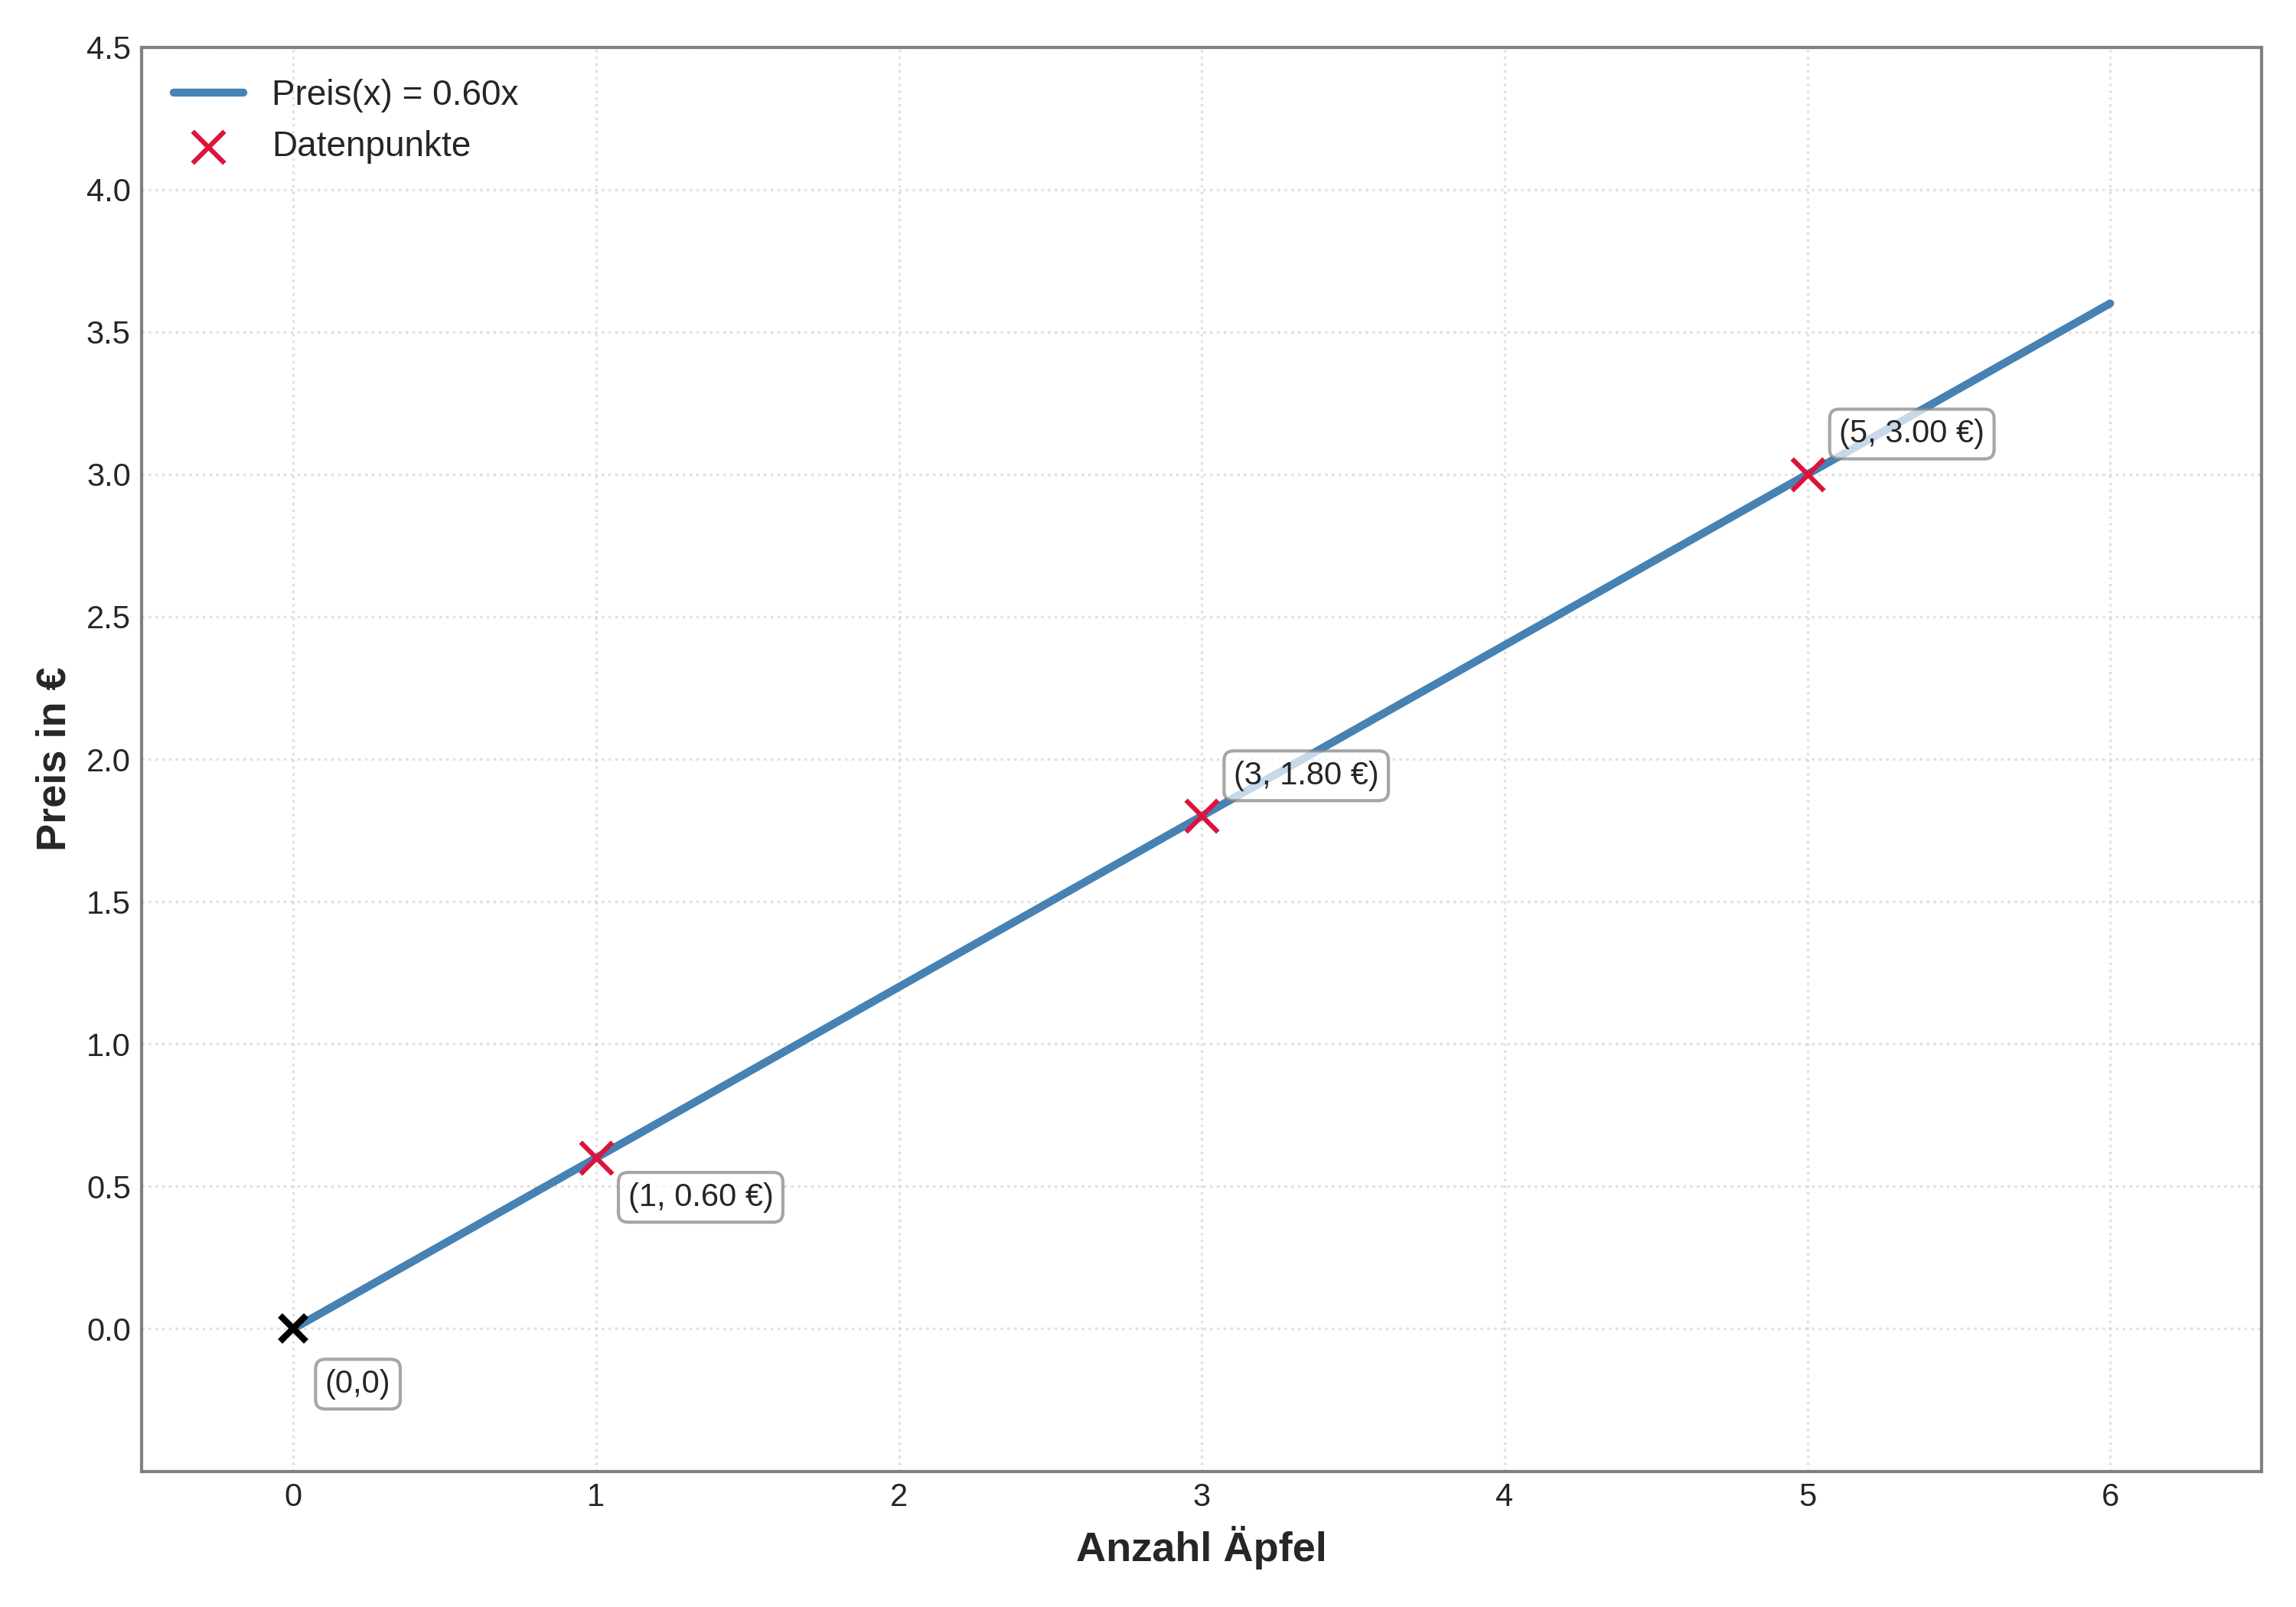
\includegraphics[width=0.8\textwidth]{grafiken/Dreisatz_Apfelpreis_Funktion.png}
    \caption{Preis für Äpfel als lineare Funktion} % \captionof{figure} wird zu \caption innerhalb der figure-Umgebung
    \label{fig:dreisatz_apfel_funktion}
\end{figure}

Dieser Übergang vom konkreten Rechnen mit dem Dreisatz zur abstrakteren Darstellung mit Funktionen ist ein wichtiger Schritt in der Mathematik. Im nächsten Kapitel schauen wir uns lineare Funktionen noch viel genauer an!
\section{Lineare Funktionen – Geraden verstehen}
\label{sec:lineare_funktionen_ueberarbeitet}

\begin{aufgabenumgebung}{Funktionsmaschinen-Logik}{}
Stell dir die folgenden Funktionsmaschinen vor. Gib jeweils die Funktionsgleichung $f(x) = \dots$ an, die beschreibt, was die Maschine mit der Eingabe $x$ macht.
\begin{enumerate}
    \item Maschine M1: Verdoppelt die Eingabe $x$ und addiert anschließend 5.
    \item Maschine M2: Subtrahiert von der Eingabe $x$ die Zahl 7 und multipliziert das Ergebnis mit 3.
    \item Maschine M3: Multipliziert die Eingabe $x$ mit sich selbst (quadriert sie) und zieht dann 4 ab.
    \item Maschine M4: Addiert zur Eingabe $x$ die Zahl 2, dividiert das Ergebnis durch 4 und addiert dann $x$.
\end{enumerate}
\end{aufgabenumgebung}


\begin{loesungsumgebung}[loes:funktionsmaschinen]{Funktionsmaschinen-Logik}
Um die Funktionsgleichungen $f(x)$ für die gegebenen Maschinen zu finden, übersetzen wir die beschriebenen Rechenschritte systematisch in mathematische Ausdrücke. Die Eingabe wird als $x$ bezeichnet.

\begin{enumerate}
    \item \textbf{Maschine M1: Verdoppelt die Eingabe $x$ und addiert anschließend 5.}
    \begin{itemize}
        \item \textbf{Schritt 1:} Die Eingabe $x$ wird verdoppelt: $2 \cdot x = 2x$.
        \item \textbf{Schritt 2:} Zu diesem Ergebnis wird 5 addiert: $2x + 5$.
    \end{itemize}
    Somit lautet die Funktionsgleichung für Maschine M1:
    $f(x) = 2x + 5$.

    \item \textbf{Maschine M2: Subtrahiert von der Eingabe $x$ die Zahl 7 und multipliziert das Ergebnis mit 3.}
    \begin{itemize}
        \item \textbf{Schritt 1:} Von der Eingabe $x$ wird 7 subtrahiert: $x - 7$.
        \item \textbf{Schritt 2:} Das Ergebnis $(x-7)$ wird mit 3 multipliziert: $3 \cdot (x - 7)$.
    \end{itemize}
    Die Funktionsgleichung für Maschine M2 ist:
    $f(x) = 3(x - 7)$.
    Man kann dies auch ausmultiplizieren zu $f(x) = 3x - 21$.

    \item \textbf{Maschine M3: Multipliziert die Eingabe $x$ mit sich selbst (quadriert sie) und zieht dann 4 ab.}
    \begin{itemize}
        \item \textbf{Schritt 1:} Die Eingabe $x$ wird mit sich selbst multipliziert (quadriert): $x \cdot x = x^2$.
        \item \textbf{Schritt 2:} Von diesem Ergebnis wird 4 abgezogen: $x^2 - 4$.
    \end{itemize}
    Die Funktionsgleichung für Maschine M3 lautet:
    $f(x) = x^2 - 4$.

    \item \textbf{Maschine M4: Addiert zur Eingabe $x$ die Zahl 2, dividiert das Ergebnis durch 4 und addiert dann $x$.}
    \begin{itemize}
        \item \textbf{Schritt 1:} Zur Eingabe $x$ wird 2 addiert: $x + 2$.
        \item \textbf{Schritt 2:} Das Ergebnis $(x+2)$ wird durch 4 dividiert: $\frac{x+2}{4}$.
        \item \textbf{Schritt 3:} Zu diesem Ergebnis wird $x$ addiert: $\frac{x+2}{4} + x$.
    \end{itemize}
    Die Funktionsgleichung für Maschine M4 ist:
    $f(x) = \frac{x+2}{4} + x$.
    Diese Gleichung kann noch vereinfacht werden:
    $f(x) = \frac{x+2}{4} + \frac{4x}{4} = \frac{x+2+4x}{4} = \frac{5x+2}{4}$.
    Alternativ kann man schreiben: $f(x) = \frac{5}{4}x + \frac{2}{4} = \frac{5}{4}x + \frac{1}{2}$.
\end{enumerate}

\begin{tippumgebung}{Text in Mathematik übersetzen}
Das Aufstellen von Funktionsgleichungen aus Textbeschreibungen ist eine wichtige Fähigkeit. Achte genau auf Schlüsselwörter:
\begin{itemize}
    \item 'addieren', 'summe', 'vermehrt um' bedeuten $+$.
    \item 'subtrahieren', 'differenz', 'vermindert um', 'zieht ab' bedeuten $-$.
    \item 'multiplizieren', 'produkt', 'mal', 'vervielfacht' bedeuten $\cdot$.
    \item 'dividieren', 'quotient', 'geteilt durch' bedeuten $: $ oder $\frac{\dots}{\dots}$.
    \item 'das Ergebnis' oder 'davon' deutet oft auf die Notwendigkeit von Klammern hin, um die Reihenfolge der Operationen korrekt wiederzugeben (Punkt- vor Strichrechnung beachten!).
\end{itemize}
Übe, die beschriebenen Schritte nacheinander in mathematische Terme umzuwandeln.
\end{tippumgebung}

\end{loesungsumgebung}

\begin{aufgabenumgebung}{Werte aus der Maschine}{}
Gegeben sind die folgenden Funktionsmaschinen durch ihre Funktionsgleichungen. Welche Ausgabe $f(x)$ (oder $y$) erzeugt die Maschine, wenn die angegebene Zahl $x$ eingegeben wird?
\begin{enumerate}
    \item $f(x) = 4x - 7$
    \begin{itemize}
        \item Was kommt raus bei $x=3$?
        \item Was kommt raus bei $x=0$?
        \item Was kommt raus bei $x=-2$?
    \end{itemize}
    \item $g(x) = -2(x+3)$
    \begin{itemize}
        \item Was kommt raus bei $x=1$?
        \item Was kommt raus bei $x=-3$?
        \item Was kommt raus bei $x=-5$?
    \end{itemize}
\end{enumerate}
\end{aufgabenumgebung}


\begin{loesungsumgebung}[loes:werte-aus-maschine]{Werte aus der Maschine}
Um die Ausgabe $f(x)$ (oder $y$) der Funktionsmaschinen zu bestimmen, setzen wir die gegebenen $x$-Werte in die jeweilige Funktionsgleichung ein und berechnen das Ergebnis.

\begin{enumerate}
    \item \textbf{Funktionsmaschine $f(x) = 4x - 7$}
    \begin{itemize}
        \item \textbf{Was kommt raus bei $x=3$?} \\
        Wir setzen $x=3$ in die Funktionsgleichung ein:
        $f(3) = 4 \cdot (3) - 7$
        $f(3) = 12 - 7$
        $f(3) = 5$ \\
        \textbf{Antwort:} Bei $x=3$ kommt $5$ raus.

        \item \textbf{Was kommt raus bei $x=0$?} \\
        Wir setzen $x=0$ in die Funktionsgleichung ein:
        $f(0) = 4 \cdot (0) - 7$
        $f(0) = 0 - 7$
        $f(0) = -7$ \\
        \textbf{Antwort:} Bei $x=0$ kommt $-7$ raus.

        \item \textbf{Was kommt raus bei $x=-2$?} \\
        Wir setzen $x=-2$ in die Funktionsgleichung ein:
        $f(-2) = 4 \cdot (-2) - 7$
        $f(-2) = -8 - 7$
        $f(-2) = -15$ \\
        \textbf{Antwort:} Bei $x=-2$ kommt $-15$ raus.
    \end{itemize}

    \item \textbf{Funktionsmaschine $g(x) = -2(x+3)$}
    \begin{itemize}
        \item \textbf{Was kommt raus bei $x=1$?} \\
        Wir setzen $x=1$ in die Funktionsgleichung ein:
        $g(1) = -2 \cdot (1+3)$
        $g(1) = -2 \cdot (4)$
        $g(1) = -8$ \\
        \textbf{Antwort:} Bei $x=1$ kommt $-8$ raus.

        \item \textbf{Was kommt raus bei $x=-3$?} \\
        Wir setzen $x=-3$ in die Funktionsgleichung ein:
        $g(-3) = -2 \cdot (-3+3)$
        $g(-3) = -2 \cdot (0)$
        $g(-3) = 0$ \\
        \textbf{Antwort:} Bei $x=-3$ kommt $0$ raus.

        \item \textbf{Was kommt raus bei $x=-5$?} \\
        Wir setzen $x=-5$ in die Funktionsgleichung ein:
        $g(-5) = -2 \cdot (-5+3)$
        $g(-5) = -2 \cdot (-2)$
        $g(-5) = 4$ \\
        \textbf{Antwort:} Bei $x=-5$ kommt $4$ raus.
    \end{itemize}
\end{enumerate}

\begin{tippumgebung}{Sorgfältiges Rechnen}
Achte beim Einsetzen von Werten in Funktionsgleichungen besonders auf:
\begin{itemize}
    \item \textbf{Klammern:} Setze negative Zahlen oder Terme, die aus mehreren Teilen bestehen (wie $(x+3)$ in $g(x)$), beim Einsetzen und Multiplizieren ggf. in Klammern, um Vorzeichenfehler zu vermeiden.
    \item \textbf{Rechenreihenfolge:} Beachte die Regel 'Punktrechnung vor Strichrechnung' und die korrekte Auswertung von Klammern. Bei $g(x) = -2(x+3)$ wird zuerst die Klammer $(x+3)$ berechnet und dann das Ergebnis mit $-2$ multipliziert.
    \item \textbf{Vorzeichen:} Sei besonders wachsam bei Rechnungen mit negativen Zahlen. $- \cdot - = +$, $+ \cdot - = -$.
\end{itemize}
Ein schrittweises Vorgehen hilft, Fehler zu minimieren.
\end{tippumgebung}

\end{loesungsumgebung}

\begin{aufgabenumgebung}{Steigung zwischen zwei Punkten}
Berechne die Steigung der Geraden, die durch die folgenden Punktepaare verläuft. Versuche auch, dir vorzustellen oder zu skizzieren, wie die Gerade ungefähr aussieht (steigend/fallend, steil/flach).
\begin{enumerate}
    \item $A(-1|1)$ und $B(2|7)$
    \item $C(0|4)$ und $D(3|1)$
    \item $E(-2|-3)$ und $F(4|-3)$ (Was ist hier besonders?)
    \item $G(2|1)$ und $H(2|5)$ (Was ist hier besonders? Ist das noch eine Funktion $y=f(x)$? Begründe!)
\end{enumerate}
\end{aufgabenumgebung}


\begin{loesungsumgebung}[loes:steigung-zwei-punkte]{Steigung zwischen zwei Punkten}
Die Steigung $m$ einer Geraden, die durch zwei Punkte $P_1(x_1|y_1)$ und $P_2(x_2|y_2)$ verläuft, wird mit der folgenden Formel berechnet:
$$ m = \frac{\Delta y}{\Delta x} = \frac{y_2 - y_1}{x_2 - x_1} $$
Diese Formel gibt das Verhältnis der Veränderung in der $y$-Richtung zur Veränderung in der $x$-Richtung an.

\begin{enumerate}
    \item \textbf{Punkte $A(-1|1)$ und $B(2|7)$} \\
    Hier ist $x_1 = -1$, $y_1 = 1$ und $x_2 = 2$, $y_2 = 7$.
    $$ m = \frac{7 - 1}{2 - (-1)} = \frac{6}{2 + 1} = \frac{6}{3} = 2 $$
    \textbf{Interpretation:} Die Steigung ist $m=2$. Da $m > 0$, ist die Gerade steigend. Für jede Einheit, die man auf der $x$-Achse nach rechts geht, geht es 2 Einheiten auf der $y$-Achse nach oben. Die Gerade ist relativ steil.

    \item \textbf{Punkte $C(0|4)$ und $D(3|1)$} \\
    Hier ist $x_1 = 0$, $y_1 = 4$ und $x_2 = 3$, $y_2 = 1$.
    $$ m = \frac{1 - 4}{3 - 0} = \frac{-3}{3} = -1 $$
    \textbf{Interpretation:} Die Steigung ist $m=-1$. Da $m < 0$, ist die Gerade fallend. Für jede Einheit, die man auf der $x$-Achse nach rechts geht, geht es 1 Einheit auf der $y$-Achse nach unten. Die Gerade fällt in einem 45°-Winkel.

    \item \textbf{Punkte $E(-2|-3)$ und $F(4|-3)$} \\
    Hier ist $x_1 = -2$, $y_1 = -3$ und $x_2 = 4$, $y_2 = -3$.
    $$ m = \frac{-3 - (-3)}{4 - (-2)} = \frac{-3 + 3}{4 + 2} = \frac{0}{6} = 0 $$
    \textbf{Was ist hier besonders?} Die Steigung ist $m=0$.
    \textbf{Interpretation:} Eine Steigung von Null bedeutet, dass die Gerade horizontal verläuft. Sie ist parallel zur $x$-Achse. Alle Punkte auf dieser Geraden haben denselben $y$-Wert (hier $y=-3$).

    \item \textbf{Punkte $G(2|1)$ und $H(2|5)$} \\
    Hier ist $x_1 = 2$, $y_1 = 1$ und $x_2 = 2$, $y_2 = 5$.
    $$ m = \frac{5 - 1}{2 - 2} = \frac{4}{0} $$
    \textbf{Was ist hier besonders?} Der Nenner ist Null, was bedeutet, dass die Steigung nicht definiert ist (Division durch Null).
    \textbf{Interpretation:} Eine undefinierte Steigung bedeutet, dass die Gerade vertikal verläuft. Sie ist parallel zur $y$-Achse. Alle Punkte auf dieser Geraden haben denselben $x$-Wert (hier $x=2$).
    \textbf{Ist das noch eine Funktion $y=f(x)$? Begründe!}
    Nein, eine vertikale Gerade (außer sie wäre die $y$-Achse selbst, und auch dann nur eingeschränkt) ist im Allgemeinen \textbf{keine Funktion} der Form $y=f(x)$.
    \textbf{Begründung:} Bei einer Funktion $y=f(x)$ muss jedem $x$-Wert genau ein $y$-Wert zugeordnet sein. Bei dieser Geraden wird dem $x$-Wert $x=2$ jedoch mehr als ein $y$-Wert zugeordnet (z.B. $y=1$ und $y=5$). Dies verletzt die Definition einer Funktion.
\end{enumerate}

\begin{merksatzumgebung}{Interpretation der Steigung $m$}
Die Steigung $m$ einer Geraden gibt an, wie stark und in welche Richtung sich die Gerade verändert:
\begin{itemize}
    \item $m > 0$: Die Gerade steigt von links nach rechts an. Je größer $m$, desto steiler.
    \item $m < 0$: Die Gerade fällt von links nach rechts ab. Je kleiner (d.h. je größer der Betrag von $m$), desto steiler fällt sie.
    \item $m = 0$: Die Gerade ist horizontal (parallel zur $x$-Achse). Die $y$-Werte ändern sich nicht.
    \item $m$ ist undefiniert (Division durch Null im Steigungsbruch): Die Gerade ist vertikal (parallel zur $y$-Achse). Die $x$-Werte ändern sich nicht. Dies ist keine Funktion $y=f(x)$.
\end{itemize}
\end{merksatzumgebung}

\begin{center}
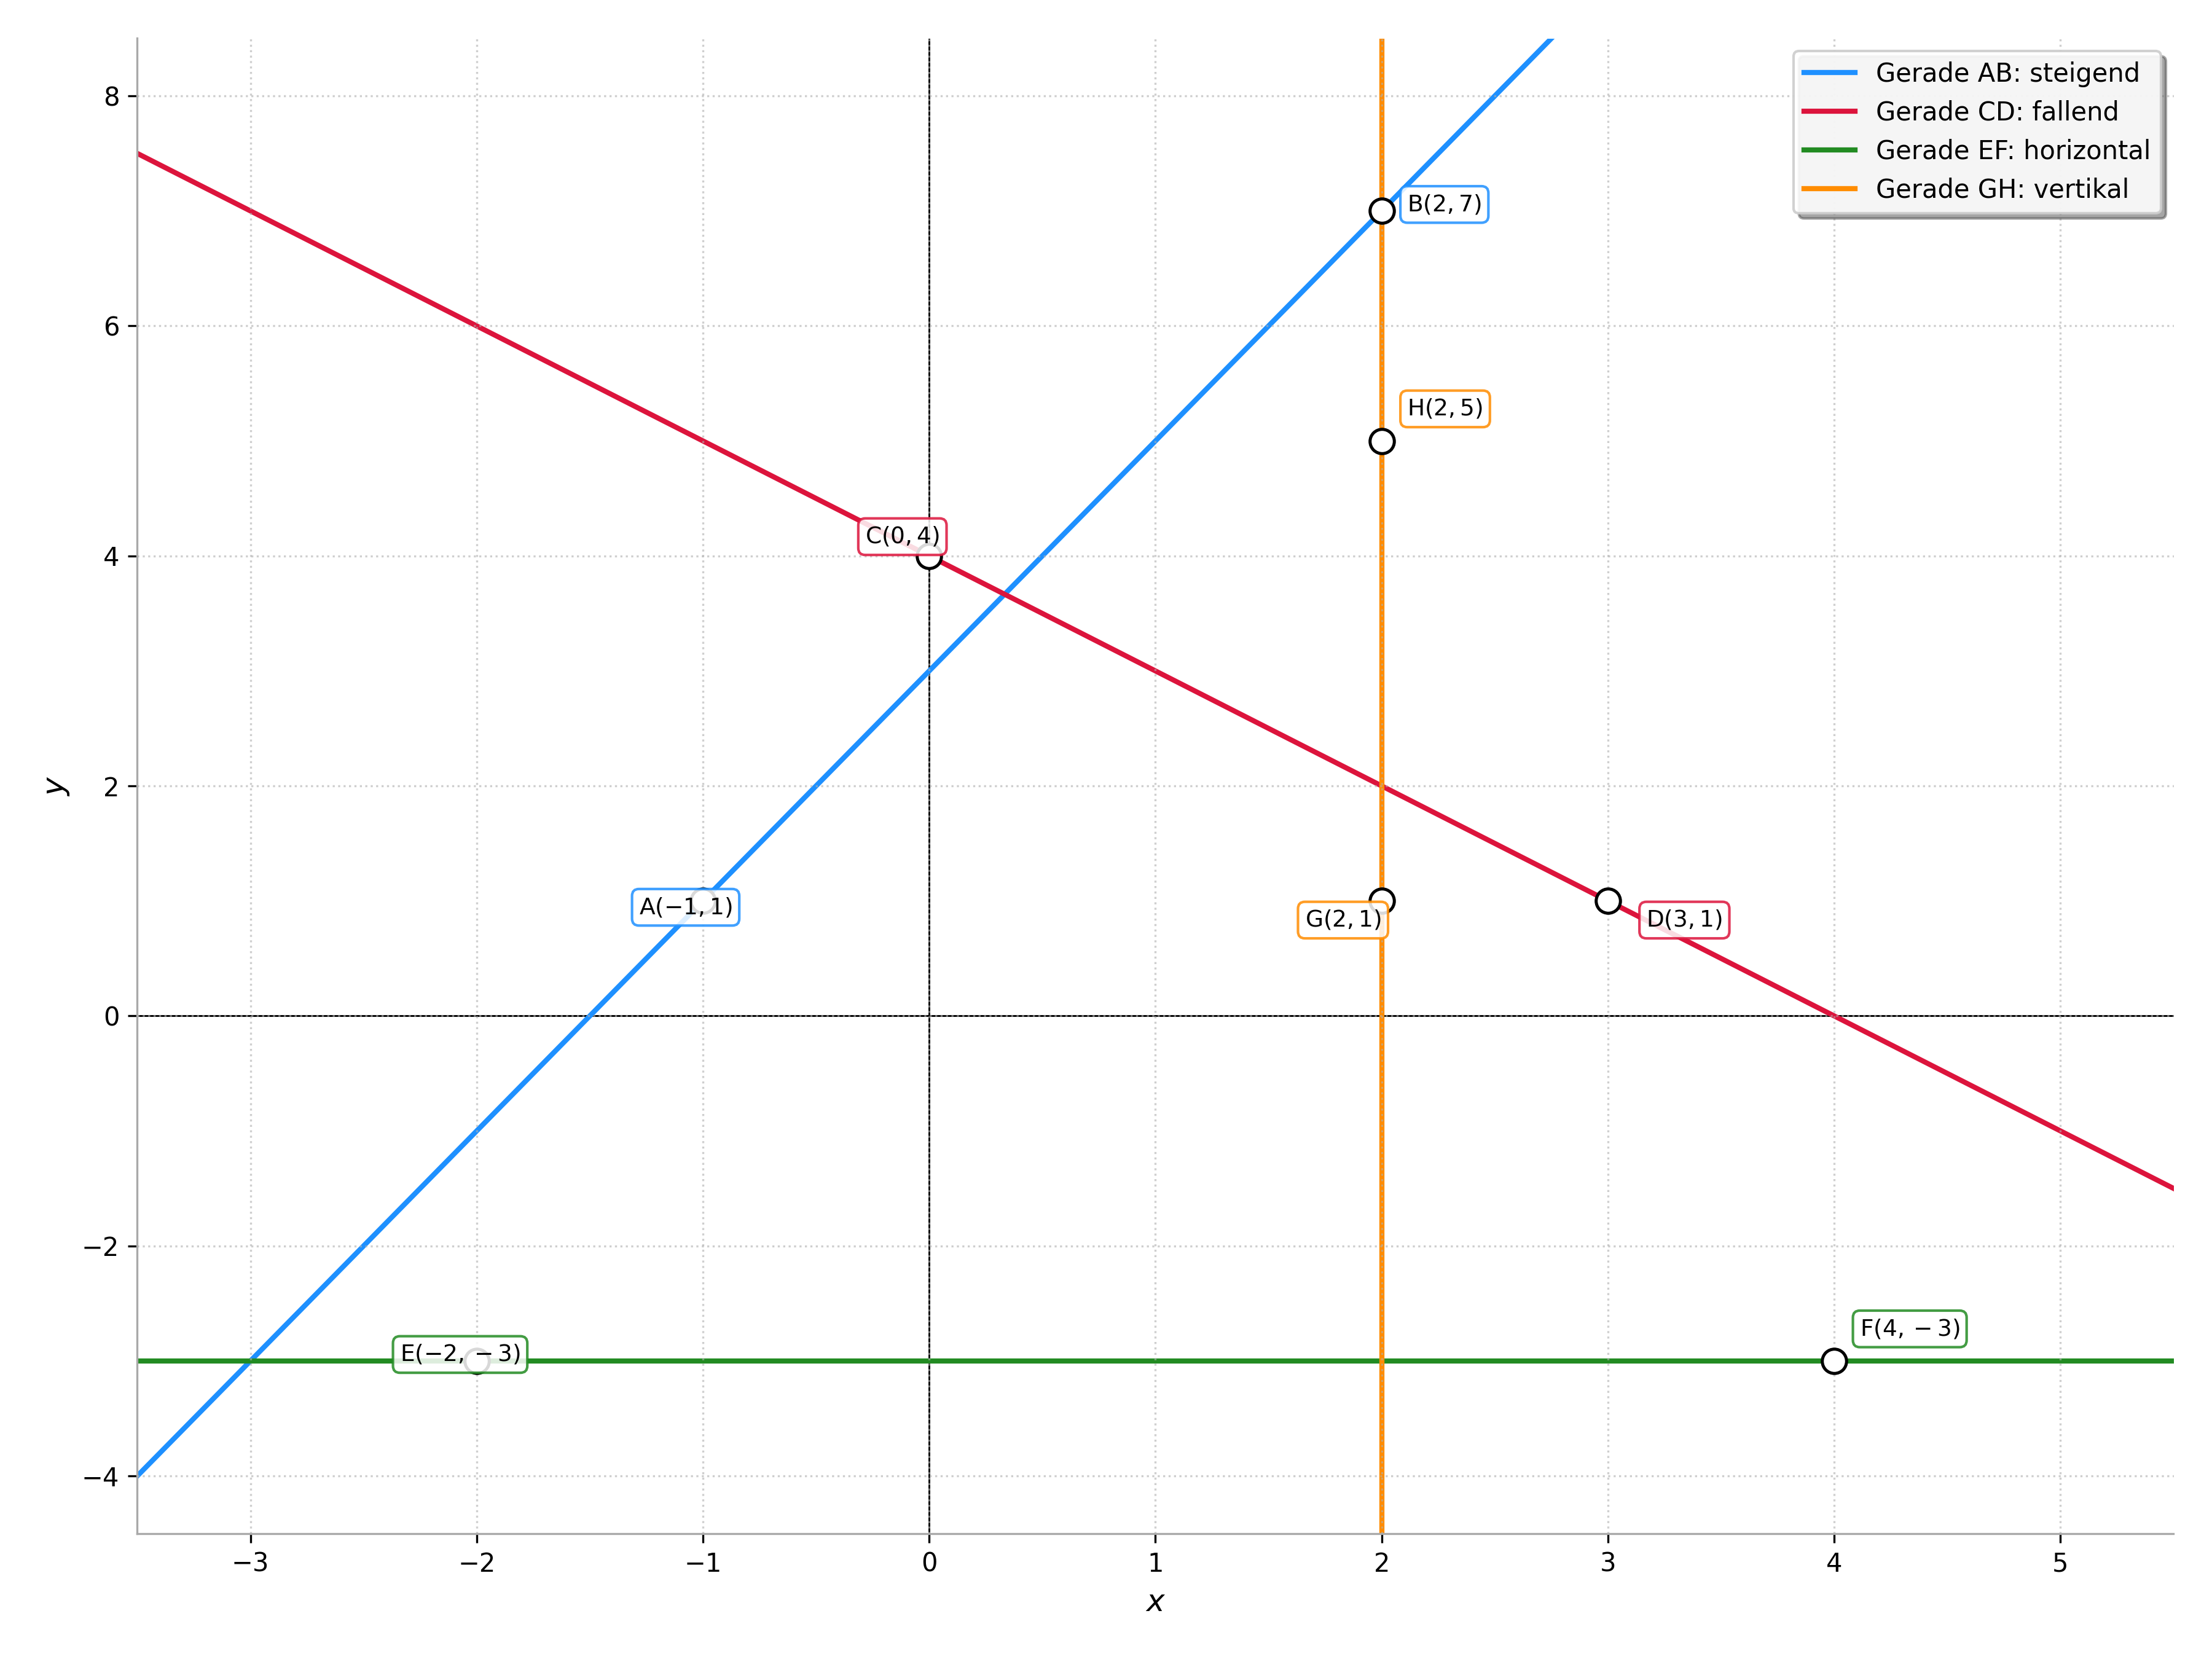
\includegraphics[width=0.9\textwidth]{grafiken/steigung_punkte_skizze.png}
% --- Beschreibung der Grafik, die hier erscheinen soll ---
% Die Grafik sollte ein Koordinatensystem zeigen, in dem die vier Geraden skizziert sind:
% 1. Gerade AB: Durch A(-1|1) und B(2|7), klar steigend.
% 2. Gerade CD: Durch C(0|4) und D(3|1), fallend.
% 3. Gerade EF: Durch E(-2|-3) und F(4|-3), horizontal.
% 4. Gerade GH: Durch G(2|1) und H(2|5), vertikal.
% Jeder Punkt sollte beschriftet sein, und die Geraden könnten farblich unterschieden oder ebenfalls beschriftet werden.
% Alternativ können auch vier separate kleine Koordinatensysteme für jede Gerade gezeichnet werden.
% Wichtig ist die visuelle Darstellung der unterschiedlichen Steigungsarten.
\captionof{figure}{Skizzen der Geraden durch die gegebenen Punktepaare zur Veranschaulichung der Steigungen.}
\label{fig:steigung_skizzen}
\end{center}

\end{loesungsumgebung}



\begin{aufgabenumgebung}{Lineare Funktionen umfassend bestimmen und analysieren}

\textbf{Teil 1: Gerade mit positiver Steigung} \\
Gegeben sind die Punkte $C(-2|0)$ und $D(2|8)$, durch die eine lineare Funktion $f(x) = ax+b$ verläuft.

\begin{enumerate}[label=(\alph*)]
    \item \textbf{Steigung berechnen:} Berechne die Steigung $a$ der Geraden durch die Punkte C und D.
    \item \textbf{Y-Achsenabschnitt berechnen:} Bestimme den y-Achsenabschnitt $b$ der Geraden.
    \item \textbf{Funktionsgleichung aufstellen:} Gib die vollständige Funktionsgleichung $f(x)$ an.
    \item \textbf{Nullstelle bestimmen:} Berechne die Nullstelle $x_N$ der Funktion $f(x)$. Welcher der gegebenen Punkte entspricht der Nullstelle?
    \item \textbf{Funktionswerte berechnen:}
        \begin{itemize}
            \item Welchen Wert hat $f(0)$? Was sagt dieser Wert über den Graphen aus?
            \item Berechne $f(1)$.
        \end{itemize}
    \item \textbf{Argument für einen Funktionswert finden:} Für welchen Wert von $x$ gilt $f(x) = 6$?
    \item \textbf{Punktprobe:} Liegt der Punkt $P(3|10)$ auf der Geraden? Begründe deine Antwort rechnerisch.
    \item \textbf{Skizze und Überprüfung:} Zeichne den Graphen der Funktion $f(x)$ in ein Koordinatensystem. Markiere die Punkte C und D sowie den y-Achsenabschnitt und die Nullstelle. Überprüfe anhand deiner Zeichnung, ob deine berechneten Werte für $a$ (Steigungsdreieck) und $b$ plausibel sind.
    \item \textbf{Vorzeichen der Funktionswerte:} Was kannst du über das Vorzeichen der Funktionswerte $f(x)$ sagen für $x$-Werte, die kleiner als die Nullstelle sind ($x < x_N$), und für $x$-Werte, die größer als die Nullstelle sind ($x > x_N$)? Begründe dies anhand der Steigung und der Nullstelle.
\end{enumerate}

\bigskip % Fügt einen größeren vertikalen Abstand ein

\textbf{Teil 2: Gerade mit negativer Steigung} \\
Gegeben sind die Punkte $E(-1|3)$ und $F(1|-1)$, durch die eine lineare Funktion $g(x) = ax+b$ verläuft.

\begin{enumerate}[label=(\alph*)]
    \item \textbf{Steigung berechnen:} Berechne die Steigung $a$ der Geraden durch die Punkte E und F.
    \item \textbf{Y-Achsenabschnitt berechnen:} Bestimme den y-Achsenabschnitt $b$ der Geraden.
    \item \textbf{Funktionsgleichung aufstellen:} Gib die vollständige Funktionsgleichung $g(x)$ an.
    \item \textbf{Nullstelle bestimmen:} Berechne die Nullstelle $x_N$ der Funktion $g(x)$.
    \item \textbf{Funktionswerte berechnen:}
        \begin{itemize}
            \item Welchen Wert hat $g(0)$? Was sagt dieser Wert über den Graphen aus?
            \item Berechne $g(3)$.
        \end{itemize}
    \item \textbf{Argument für einen Funktionswert finden:} Für welchen Wert von $x$ gilt $g(x) = 7$?
    \item \textbf{Punktprobe:} Liegt der Punkt $Q(0.5|0)$ auf der Geraden? Begründe deine Antwort rechnerisch. (Tipp: Vergleiche mit deiner Berechnung aus Teil d)).
    \item \textbf{Skizze und Überprüfung:} Zeichne den Graphen der Funktion $g(x)$ in ein Koordinatensystem. Markiere die Punkte E und F sowie den y-Achsenabschnitt und die Nullstelle. Überprüfe anhand deiner Zeichnung, ob deine berechneten Werte für $a$ (Ist die Gerade fallend? Wie ist das Steigungsdreieck?) und $b$ plausibel sind.
    \item \textbf{Vorzeichen der Funktionswerte:} Was kannst du über das Vorzeichen der Funktionswerte $g(x)$ sagen für $x$-Werte, die kleiner als die Nullstelle sind ($x < x_N$), und für $x$-Werte, die größer als die Nullstelle sind ($x > x_N$)? Begründe dies anhand der (negativen) Steigung und der Nullstelle.
\end{enumerate}
\end{aufgabenumgebung}


\begin{loesungsumgebung}[loes:lineare-funktionen-umfassend]{Lineare Funktionen umfassend bestimmen und analysieren}

\subsection*{Teil 1: Gerade mit positiver Steigung durch $C(-2|0)$ und $D(2|8)$}
Die allgemeine Form einer linearen Funktion ist $f(x) = ax+b$.

\begin{enumerate}[label=(\alph*)]
    \item \textbf{Steigung berechnen:}
    Die Punkte sind $C(-2|0)$ (also $x_1=-2, y_1=0$) und $D(2|8)$ (also $x_2=2, y_2=8$).
    Die Steigung $a$ berechnet sich als:
    $$ a = \frac{y_2 - y_1}{x_2 - x_1} = \frac{8 - 0}{2 - (-2)} = \frac{8}{2+2} = \frac{8}{4} = 2 $$
    Die Steigung ist $a=2$.

    \item \textbf{Y-Achsenabschnitt berechnen:}
    Wir setzen die Steigung $a=2$ und die Koordinaten eines Punktes (z.B. $D(2|8)$) in die Funktionsgleichung $f(x) = ax+b$ ein:
    $8 = 2 \cdot (2) + b$
    $8 = 4 + b$
    $b = 8 - 4 = 4$
    Der y-Achsenabschnitt ist $b=4$.

    \item \textbf{Funktionsgleichung aufstellen:}
    Mit $a=2$ und $b=4$ lautet die Funktionsgleichung:
    $f(x) = 2x + 4$.

    \item \textbf{Nullstelle bestimmen:}
    Die Nullstelle $x_N$ ist der $x$-Wert, für den $f(x_N)=0$ gilt:
    $2x_N + 4 = 0$
    $2x_N = -4$
    $x_N = -2$
    Die Nullstelle ist $x_N = -2$.
    Der gegebene Punkt $C(-2|0)$ entspricht der Nullstelle, da sein $y$-Wert 0 ist.

    \item \textbf{Funktionswerte berechnen:}
    \begin{itemize}
        \item Welchen Wert hat $f(0)$?
        $f(0) = 2 \cdot (0) + 4 = 0 + 4 = 4$.
        Was sagt dieser Wert über den Graphen aus? Der Wert $f(0)=4$ ist der y-Achsenabschnitt $b$. Er gibt an, dass der Graph die y-Achse im Punkt $(0|4)$ schneidet.
        \item Berechne $f(1)$.
        $f(1) = 2 \cdot (1) + 4 = 2 + 4 = 6$.
    \end{itemize}

    \item \textbf{Argument für einen Funktionswert finden:} Für welchen Wert von $x$ gilt $f(x) = 6$?
    $2x + 4 = 6$
    $2x = 6 - 4$
    $2x = 2$
    $x = 1$
    Für $x=1$ gilt $f(x)=6$.

    \item \textbf{Punktprobe:} Liegt der Punkt $P(3|10)$ auf der Geraden?
    Wir setzen $x=3$ in die Funktionsgleichung $f(x) = 2x+4$ ein:
    $f(3) = 2 \cdot (3) + 4 = 6 + 4 = 10$.
    Da der berechnete Funktionswert $10$ mit der y-Koordinate des Punktes $P$ übereinstimmt, liegt der Punkt $P(3|10)$ auf der Geraden.

    \item \textbf{Skizze und Überprüfung:}
    \begin{center}
    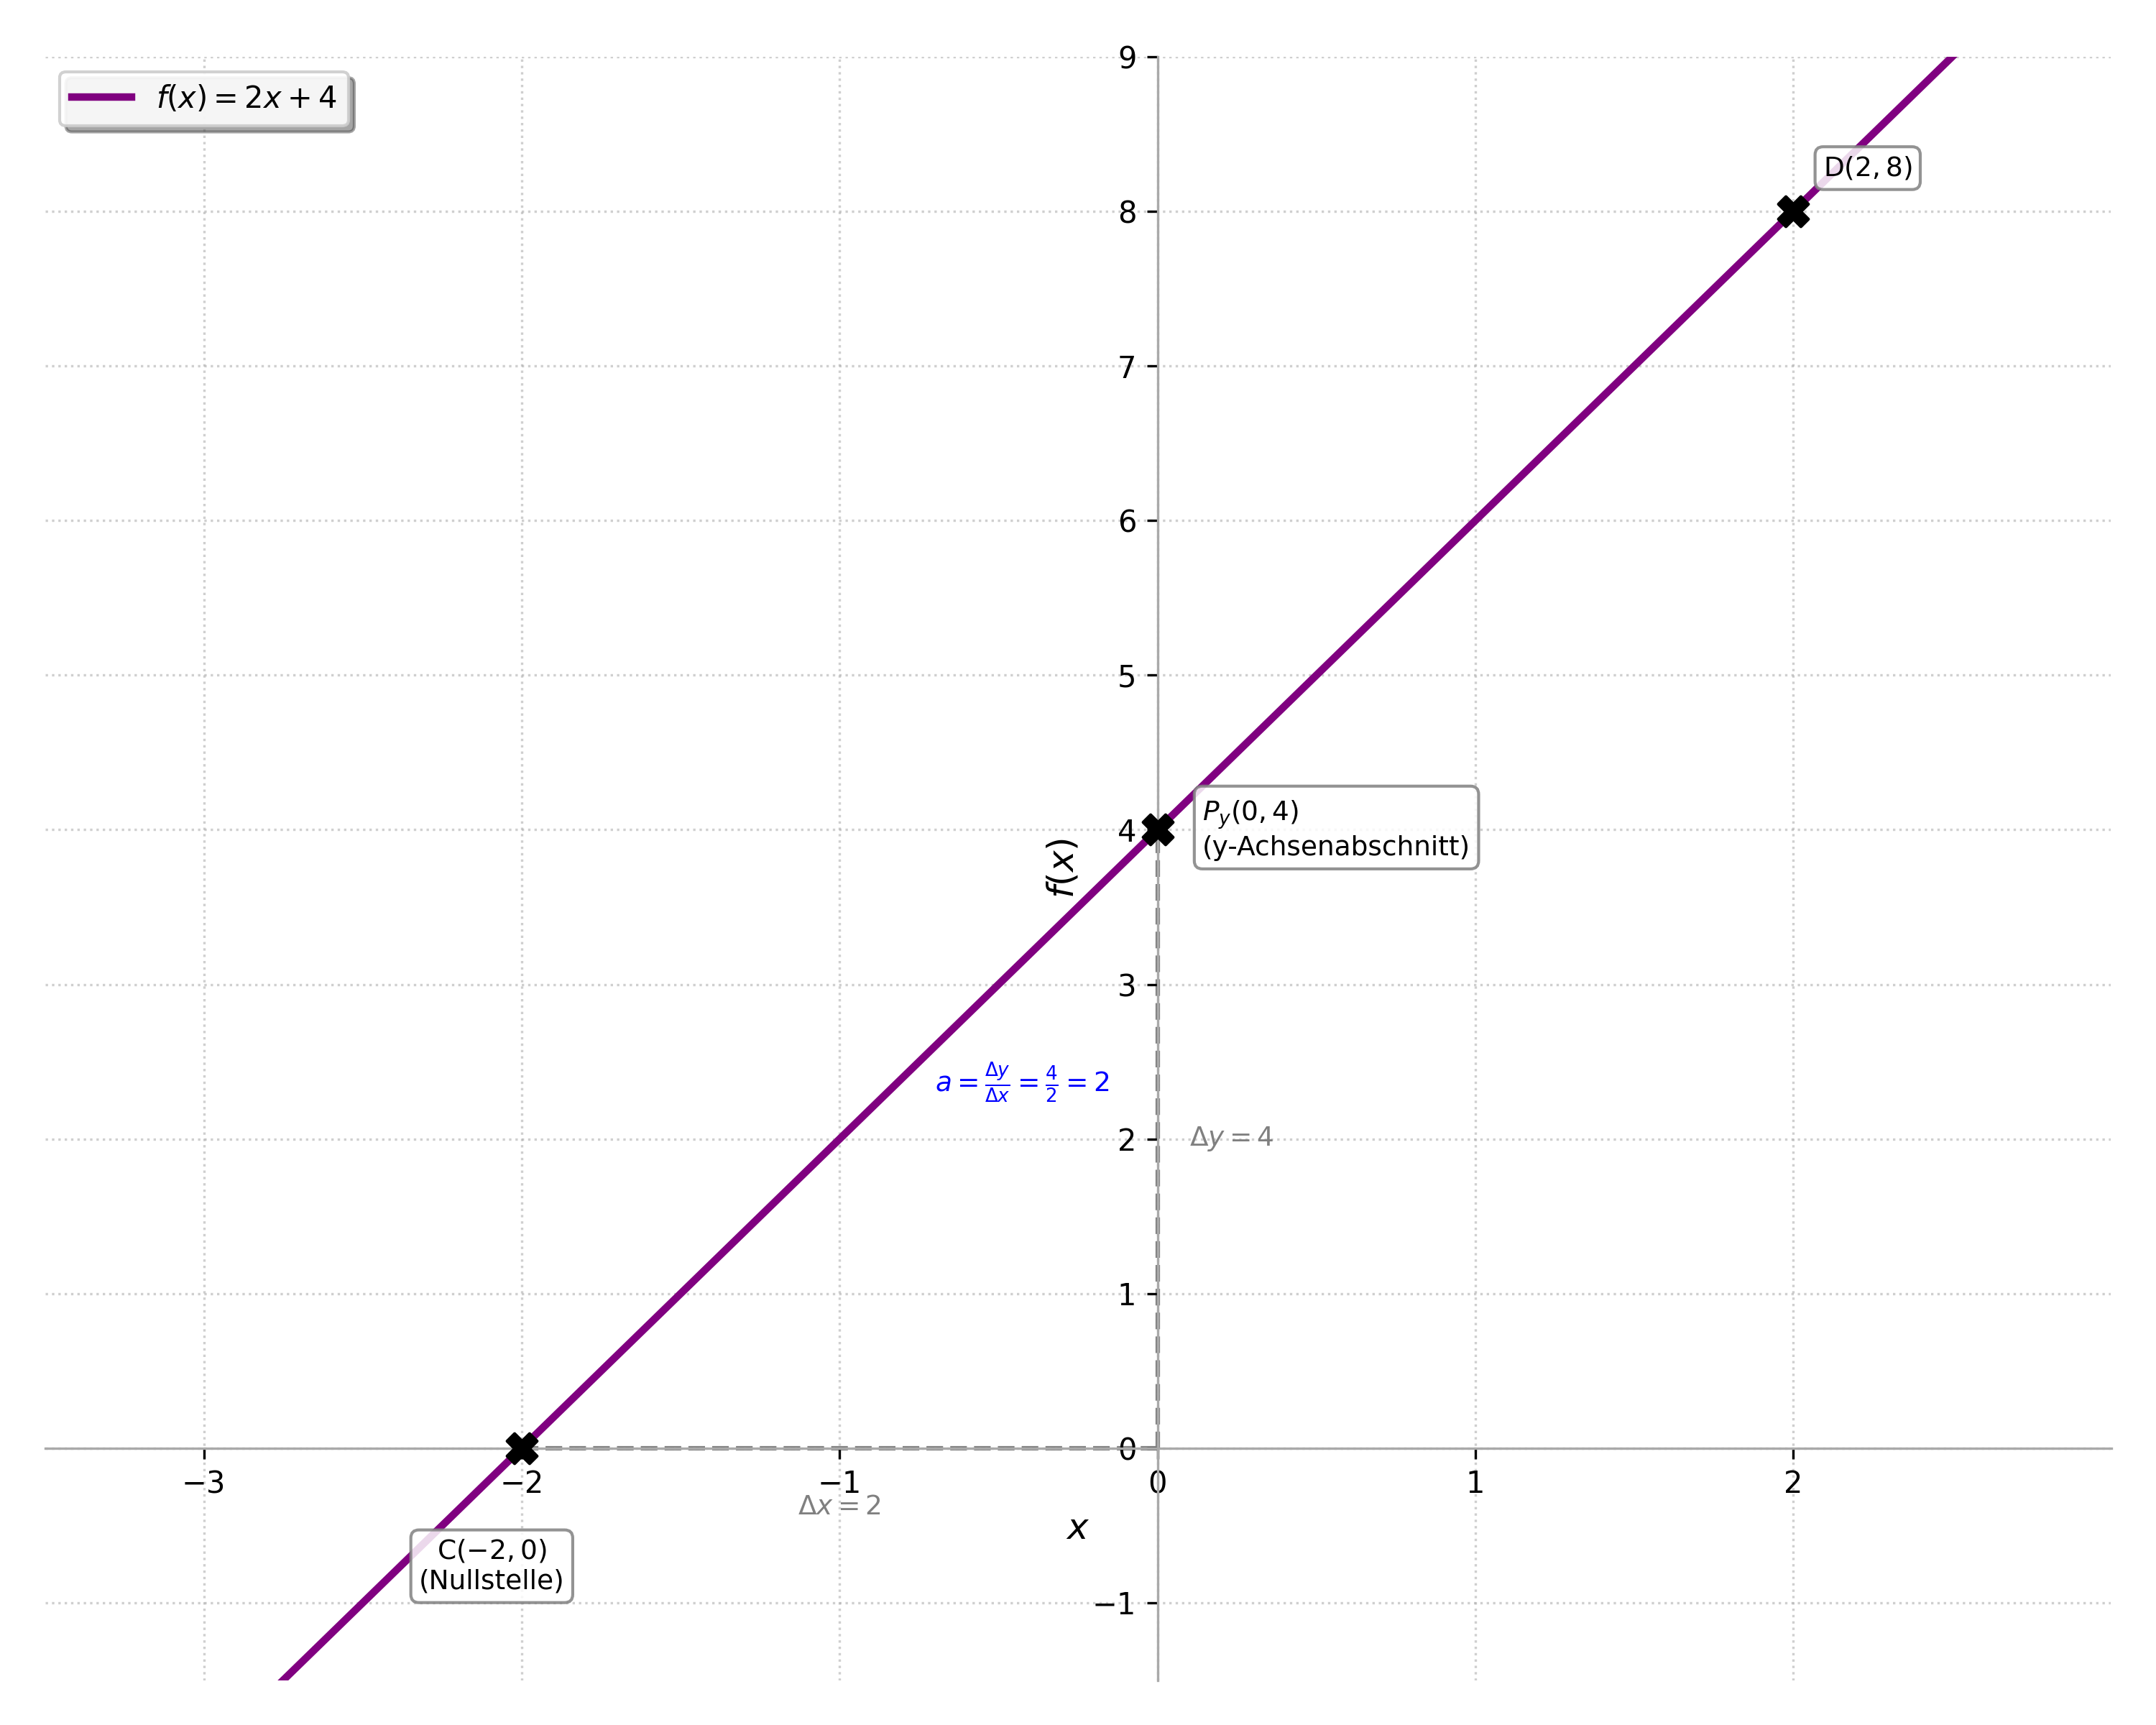
\includegraphics[width=0.8\textwidth]{grafiken/lin_fkt_teil1_skizze.png}
    % --- Beschreibung der Grafik für Teil 1 ---
    % Die Grafik sollte ein Koordinatensystem zeigen.
    % Eingezeichnet ist die Gerade f(x) = 2x + 4.
    % Die Punkte C(-2|0) und D(2|8) sind markiert.
    % Der y-Achsenabschnitt (0|4) ist markiert.
    % Die Nullstelle (-2|0) ist markiert (identisch mit Punkt C).
    % Ein Steigungsdreieck ist eingezeichnet, das die Steigung a=2 verdeutlicht (z.B. von C aus: 2 Einheiten nach rechts, 4 Einheiten nach oben bis (0|4), oder 1 Einheit nach rechts, 2 Einheiten nach oben).
    % Die Achsen sind beschriftet (x und y oder f(x)).
    \captionof{figure}{Skizze der Funktion $f(x)=2x+4$ mit Punkten C und D, y-Achsenabschnitt und Nullstelle.}
    \label{fig:lin_fkt_teil1}
    \end{center}
    \textbf{Überprüfung anhand der Skizze:} Man sollte erkennen, dass die Gerade durch die Punkte C und D verläuft. Der Schnittpunkt mit der y-Achse sollte bei $y=4$ liegen. Die Nullstelle (Schnittpunkt mit der x-Achse) sollte bei $x=-2$ liegen. Das Steigungsdreieck sollte eine Steigung von $a=2$ (z.B. 1 Einheit nach rechts, 2 Einheiten nach oben) visuell bestätigen. Die Gerade steigt an, was zu $a>0$ passt.

    \item \textbf{Vorzeichen der Funktionswerte:}
    Die Nullstelle ist $x_N = -2$ und die Steigung ist $a=2$ (positiv).
    \begin{itemize}
        \item Für $x < x_N$ (also $x < -2$): Die Funktionswerte $f(x)$ sind \textbf{negativ}. Da die Gerade steigt ($a>0$), kommt sie von 'unten links' und durchquert die x-Achse an der Nullstelle. Links von der Nullstelle liegen die Funktionswerte unterhalb der x-Achse. Z.B. $f(-3) = 2(-3)+4 = -2$.
        \item Für $x > x_N$ (also $x > -2$): Die Funktionswerte $f(x)$ sind \textbf{positiv}. Rechts von der Nullstelle liegen die Funktionswerte oberhalb der x-Achse. Z.B. $f(0) = 4$.
    \end{itemize}
\end{enumerate}

\bigskip % Vertikaler Abstand zwischen den Teilen

\subsection*{Teil 2: Gerade mit negativer Steigung durch $E(-1|3)$ und $F(1|-1)$}
Die allgemeine Form einer linearen Funktion ist $g(x) = ax+b$.

\begin{enumerate}[label=(\alph*)]
    \item \textbf{Steigung berechnen:}
    Die Punkte sind $E(-1|3)$ (also $x_1=-1, y_1=3$) und $F(1|-1)$ (also $x_2=1, y_2=-1$).
    Die Steigung $a$ berechnet sich als:
    $$ a = \frac{y_2 - y_1}{x_2 - x_1} = \frac{-1 - 3}{1 - (-1)} = \frac{-4}{1+1} = \frac{-4}{2} = -2 $$
    Die Steigung ist $a=-2$.

    \item \textbf{Y-Achsenabschnitt berechnen:}
    Wir setzen die Steigung $a=-2$ und die Koordinaten eines Punktes (z.B. $E(-1|3)$) in die Funktionsgleichung $g(x) = ax+b$ ein:
    $3 = -2 \cdot (-1) + b$
    $3 = 2 + b$
    $b = 3 - 2 = 1$
    Der y-Achsenabschnitt ist $b=1$.

    \item \textbf{Funktionsgleichung aufstellen:}
    Mit $a=-2$ und $b=1$ lautet die Funktionsgleichung:
    $g(x) = -2x + 1$.

    \item \textbf{Nullstelle bestimmen:}
    Die Nullstelle $x_N$ ist der $x$-Wert, für den $g(x_N)=0$ gilt:
    $-2x_N + 1 = 0$
    $-2x_N = -1$
    $x_N = \frac{-1}{-2} = \frac{1}{2}$ (oder $0.5$)
    Die Nullstelle ist $x_N = \frac{1}{2}$.

    \item \textbf{Funktionswerte berechnen:}
    \begin{itemize}
        \item Welchen Wert hat $g(0)$?
        $g(0) = -2 \cdot (0) + 1 = 0 + 1 = 1$.
        Was sagt dieser Wert über den Graphen aus? Der Wert $g(0)=1$ ist der y-Achsenabschnitt $b$. Er gibt an, dass der Graph die y-Achse im Punkt $(0|1)$ schneidet.
        \item Berechne $g(3)$.
        $g(3) = -2 \cdot (3) + 1 = -6 + 1 = -5$.
    \end{itemize}

    \item \textbf{Argument für einen Funktionswert finden:} Für welchen Wert von $x$ gilt $g(x) = 7$?
    $-2x + 1 = 7$
    $-2x = 7 - 1$
    $-2x = 6$
    $x = \frac{6}{-2} = -3$
    Für $x=-3$ gilt $g(x)=7$.

    \item \textbf{Punktprobe:} Liegt der Punkt $Q(0.5|0)$ auf der Geraden?
    Wir setzen $x=0.5$ in die Funktionsgleichung $g(x) = -2x+1$ ein:
    $g(0.5) = -2 \cdot (0.5) + 1 = -1 + 1 = 0$.
    Da der berechnete Funktionswert $0$ mit der y-Koordinate des Punktes $Q$ übereinstimmt, liegt der Punkt $Q(0.5|0)$ auf der Geraden.
    \textbf{Tipp-Vergleich:} Dies stimmt mit der Berechnung aus Teil d) überein, da $x_N=0.5$ die Nullstelle ist und $Q(0.5|0)$ somit der Nullstellenpunkt.

    \item \textbf{Skizze und Überprüfung:}
    \begin{center}
    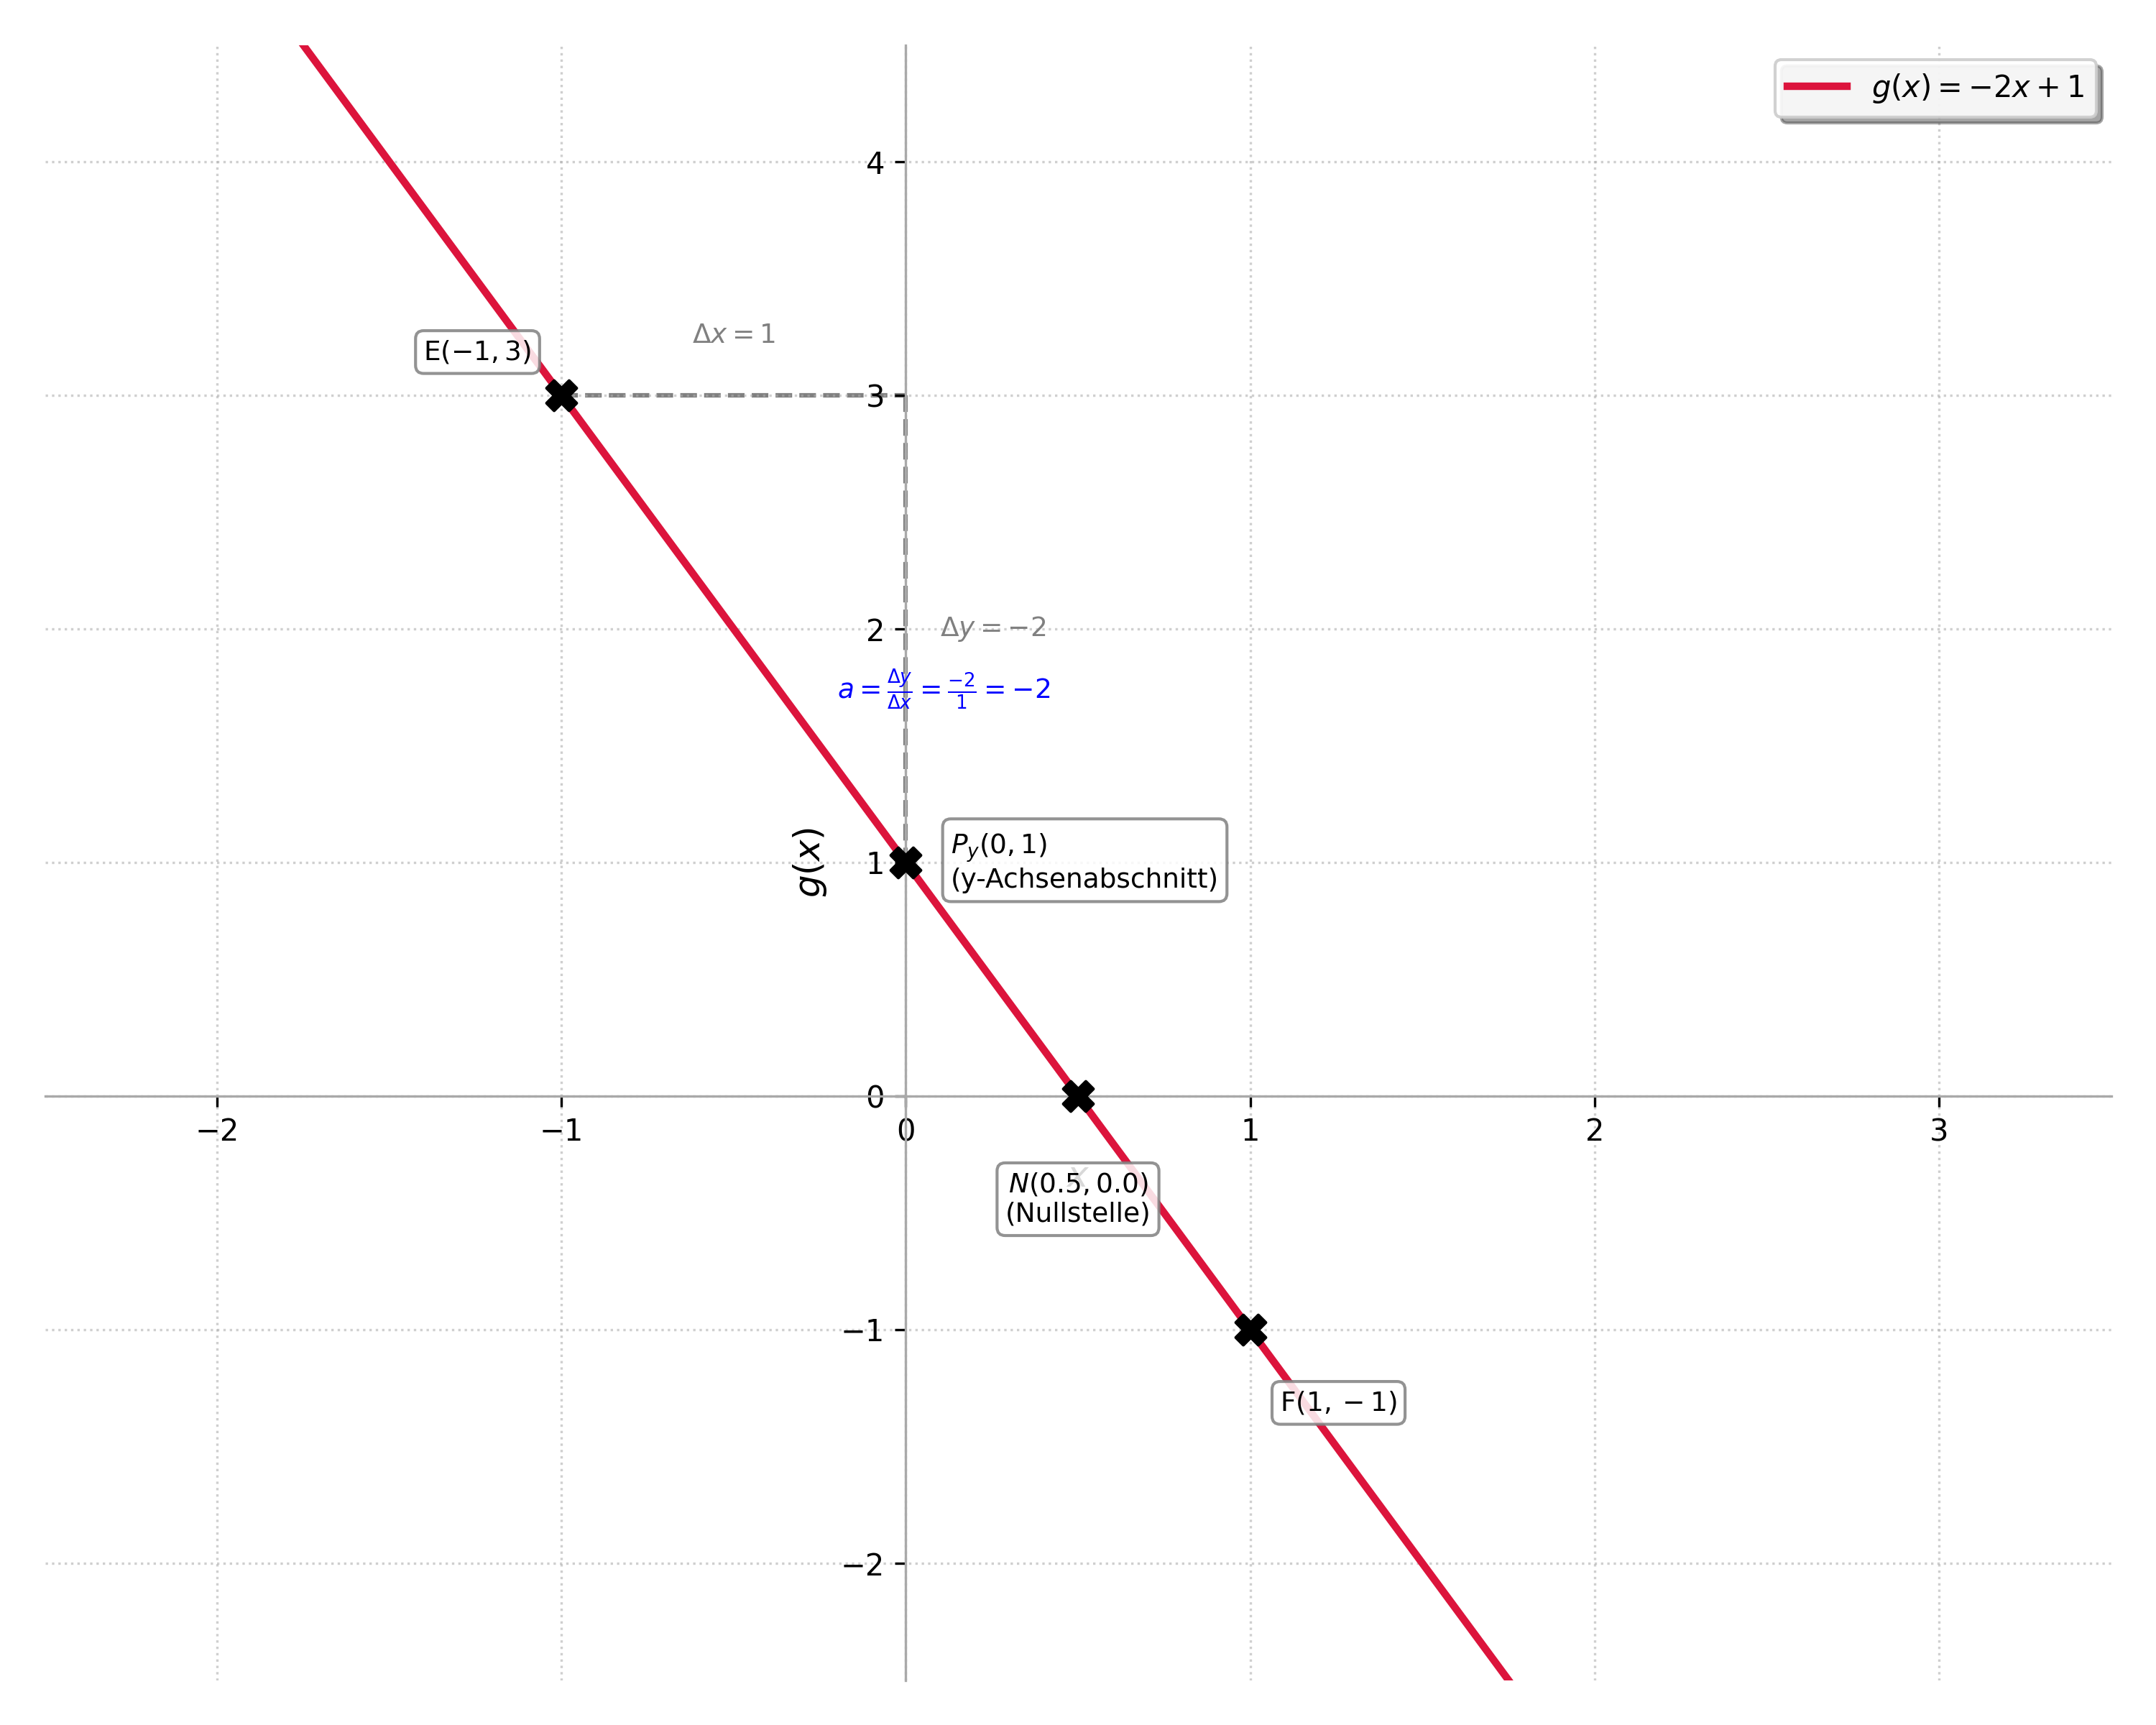
\includegraphics[width=0.8\textwidth]{grafiken/lin_fkt_teil2_skizze.png}
    % --- Beschreibung der Grafik für Teil 2 ---
    % Die Grafik sollte ein Koordinatensystem zeigen.
    % Eingezeichnet ist die Gerade g(x) = -2x + 1.
    % Die Punkte E(-1|3) und F(1|-1) sind markiert.
    % Der y-Achsenabschnitt (0|1) ist markiert.
    % Die Nullstelle (0.5|0) ist markiert.
    % Ein Steigungsdreieck ist eingezeichnet, das die Steigung a=-2 verdeutlicht (z.B. von E aus: 1 Einheit nach rechts, 2 Einheiten nach unten).
    % Die Achsen sind beschriftet (x und y oder g(x)).
    \captionof{figure}{Skizze der Funktion $g(x)=-2x+1$ mit Punkten E und F, y-Achsenabschnitt und Nullstelle.}
    \label{fig:lin_fkt_teil2}
    \end{center}
    \textbf{Überprüfung anhand der Skizze:} Man sollte erkennen, dass die Gerade durch die Punkte E und F verläuft und fallend ist ($a<0$). Der Schnittpunkt mit der y-Achse sollte bei $y=1$ liegen. Die Nullstelle sollte bei $x=0.5$ liegen. Das Steigungsdreieck sollte eine Steigung von $a=-2$ (z.B. 1 Einheit nach rechts, 2 Einheiten nach unten) visuell bestätigen.

    \item \textbf{Vorzeichen der Funktionswerte:}
    Die Nullstelle ist $x_N = \frac{1}{2}$ und die Steigung ist $a=-2$ (negativ).
    \begin{itemize}
        \item Für $x < x_N$ (also $x < \frac{1}{2}$): Die Funktionswerte $g(x)$ sind \textbf{positiv}. Da die Gerade fällt ($a<0$), kommt sie von 'oben links' und durchquert die x-Achse an der Nullstelle. Links von der Nullstelle liegen die Funktionswerte oberhalb der x-Achse. Z.B. $g(0) = 1$.
        \item Für $x > x_N$ (also $x > \frac{1}{2}$): Die Funktionswerte $g(x)$ sind \textbf{negativ}. Rechts von der Nullstelle liegen die Funktionswerte unterhalb der x-Achse. Z.B. $g(1) = -1$.
    \end{itemize}
\end{enumerate}

\end{loesungsumgebung}

\begin{aufgabenumgebung}{Nullstellen finden}
Berechne die Nullstellen der folgenden linearen Funktionen. Gib auch den Schnittpunkt mit der x-Achse an.
\begin{enumerate}
    \item $f(x) = 3x + 6$
    \item $g(x) = -0.5x + 2$
    \item $h(x) = 4x$
    \item $k(x) = 5$ (Was passiert hier?)
\end{enumerate}
\end{aufgabenumgebung}

\begin{loesungsumgebung}[loes:nullstellen-finden-mit-umformung]{Nullstellen finden}
Die Nullstelle einer Funktion ist der $x$-Wert, an dem der Funktionswert $f(x)$ gleich Null ist. Grafisch entspricht dies der x-Koordinate des Schnittpunktes des Graphen mit der x-Achse. Um die Nullstelle(n) zu berechnen, setzen wir $f(x)=0$ und lösen die Gleichung nach $x$ auf. Der Schnittpunkt mit der x-Achse hat dann die Koordinaten $(x_N|0)$, wobei $x_N$ die Nullstelle ist.

\begin{enumerate}
    \item \textbf{Funktion $f(x) = 3x + 6$} \\
    Wir setzen $f(x)=0$. Die Umformungsschritte sind:
    $$
    \begin{array}{r c l c l}
    \umformung{3x+6}{0}{-}{6}
    \umformung{3x}{-6}{\div}{3}
    \umformungend{x}{-2}
    \end{array}
    $$
    Die Nullstelle ist $x_N = -2$. \\
    Der Schnittpunkt mit der x-Achse ist $S_x(-2|0)$.

    \item \textbf{Funktion $g(x) = -0.5x + 2$} \\
    Wir setzen $g(x)=0$. Die Umformungsschritte sind:
    $$
    \begin{array}{r c l c l}
    \umformung{-0.5x + 2}{0}{-}{2}
    \umformung{-0.5x}{-2}{\div}{(-0.5)}
    \umformungend{x}{4}
    \end{array}
    $$
    Die Nullstelle ist $x_N = 4$. \\
    Der Schnittpunkt mit der x-Achse ist $S_x(4|0)$.

    \item \textbf{Funktion $h(x) = 4x$} \\
    Wir setzen $h(x)=0$. Die Umformungsschritte sind:
    $$
    \begin{array}{r c l c l}
    \umformung{4x}{0}{\div}{4}
    \umformungend{x}{0}
    \end{array}
    $$
    Die Nullstelle ist $x_N = 0$. \\
    Der Schnittpunkt mit der x-Achse ist $S_x(0|0)$. Dieser Punkt ist auch der Ursprung des Koordinatensystems und gleichzeitig der y-Achsenabschnitt.

    \item \textbf{Funktion $k(x) = 5$} \\
    Wir setzen $k(x)=0$:
    $$ 5 = 0 $$
    \textbf{Was passiert hier?} Die Gleichung $5=0$ ist eine falsche Aussage. Das bedeutet, es gibt keinen $x$-Wert, für den $k(x)=0$ wird.
    \textbf{Erklärung:} Die Funktion $k(x)=5$ ist eine konstante Funktion. Ihr Graph ist eine horizontale Gerade, die parallel zur x-Achse im Abstand von 5 Einheiten verläuft (also durch den Punkt $(0|5)$). Da diese Gerade die x-Achse niemals schneidet (es sei denn, die Konstante wäre 0), hat die Funktion keine Nullstellen. \\
    Die Funktion $k(x)=5$ hat \textbf{keine Nullstellen}. Es gibt keinen Schnittpunkt mit der x-Achse.
\end{enumerate}

\begin{merksatzumgebung}{Nullstellen und konstante Funktionen}
\begin{itemize}
    \item Eine \textbf{Nullstelle} $x_N$ einer Funktion $f$ ist ein Wert im Definitionsbereich, für den $f(x_N)=0$ gilt. Der Punkt $(x_N|0)$ ist der Schnittpunkt des Graphen mit der x-Achse.
    \item Lineare Funktionen der Form $f(x) = ax+b$ mit $a \neq 0$ haben immer genau eine Nullstelle bei $x_N = -\frac{b}{a}$.
    \item Konstante Funktionen $f(x)=c$ (wobei $c$ eine Zahl ist):
    \begin{itemize}
        \item Wenn $c \neq 0$ (wie bei $k(x)=5$), hat die Funktion \textbf{keine Nullstellen}, da ihr Graph eine horizontale Linie ist, die die x-Achse nicht schneidet.
        \item Wenn $c = 0$ (also $f(x)=0$), dann ist jeder $x$-Wert eine Nullstelle, da der Graph der Funktion die x-Achse selbst ist. In diesem Fall hat die Funktion unendlich viele Nullstellen.
    \end{itemize}
\end{itemize}
\end{merksatzumgebung}

\end{loesungsumgebung}


\begin{aufgabenumgebung}{Deine Wertetabelle}
Erstelle eine Wertetabelle für die Funktion $g(x) = -2x + 3$ für die x-Werte von -3 bis 3 in Einerschritten. Zeichne anschließend den Graphen der Funktion mithilfe der Punkte aus deiner Wertetabelle.
\end{aufgabenumgebung}


\begin{loesungsumgebung}[loes:wertetabelle-zeichnen]{Deine Wertetabelle}
Um die Wertetabelle für die Funktion $g(x) = -2x + 3$ zu erstellen, setzen wir die gegebenen x-Werte (-3, -2, -1, 0, 1, 2, 3) nacheinander in die Funktionsgleichung ein und berechnen den jeweiligen Funktionswert $g(x)$.

\textbf{Schritt 1: Funktionswerte berechnen}
\begin{itemize}
    \item Für $x = -3$: $g(-3) = -2(-3) + 3 = 6 + 3 = 9$
    \item Für $x = -2$: $g(-2) = -2(-2) + 3 = 4 + 3 = 7$
    \item Für $x = -1$: $g(-1) = -2(-1) + 3 = 2 + 3 = 5$
    \item Für $x = 0$: $g(0) = -2(0) + 3 = 0 + 3 = 3$
    \item Für $x = 1$: $g(1) = -2(1) + 3 = -2 + 3 = 1$
    \item Für $x = 2$: $g(2) = -2(2) + 3 = -4 + 3 = -1$
    \item Für $x = 3$: $g(3) = -2(3) + 3 = -6 + 3 = -3$
\end{itemize}

\textbf{Schritt 2: Wertetabelle erstellen}
Die berechneten Wertepaare $(x | g(x))$ können wir nun in einer Tabelle zusammenfassen:

\begin{center}
\begin{tabular}{r r}
\toprule
\multicolumn{1}{c}{$x$} & \multicolumn{1}{c}{$g(x) = -2x + 3$} \\
\midrule
$-3$ & $9$ \\
$-2$ & $7$ \\
$-1$ & $5$ \\
$0$ & $3$ \\
$1$ & $1$ \\
$2$ & $-1$ \\
$3$ & $-3$ \\
\bottomrule
\end{tabular}
\end{center}

\textbf{Schritt 3: Graphen der Funktion zeichnen}
Mithilfe der Punkte aus der Wertetabelle $( (-3|9), (-2|7), (-1|5), (0|3), (1|1), (2|-1), (3|-3) )$ kann nun der Graph der Funktion $g(x) = -2x+3$ gezeichnet werden. Da es sich um eine lineare Funktion handelt, liegen alle Punkte auf einer Geraden.

\begin{center}
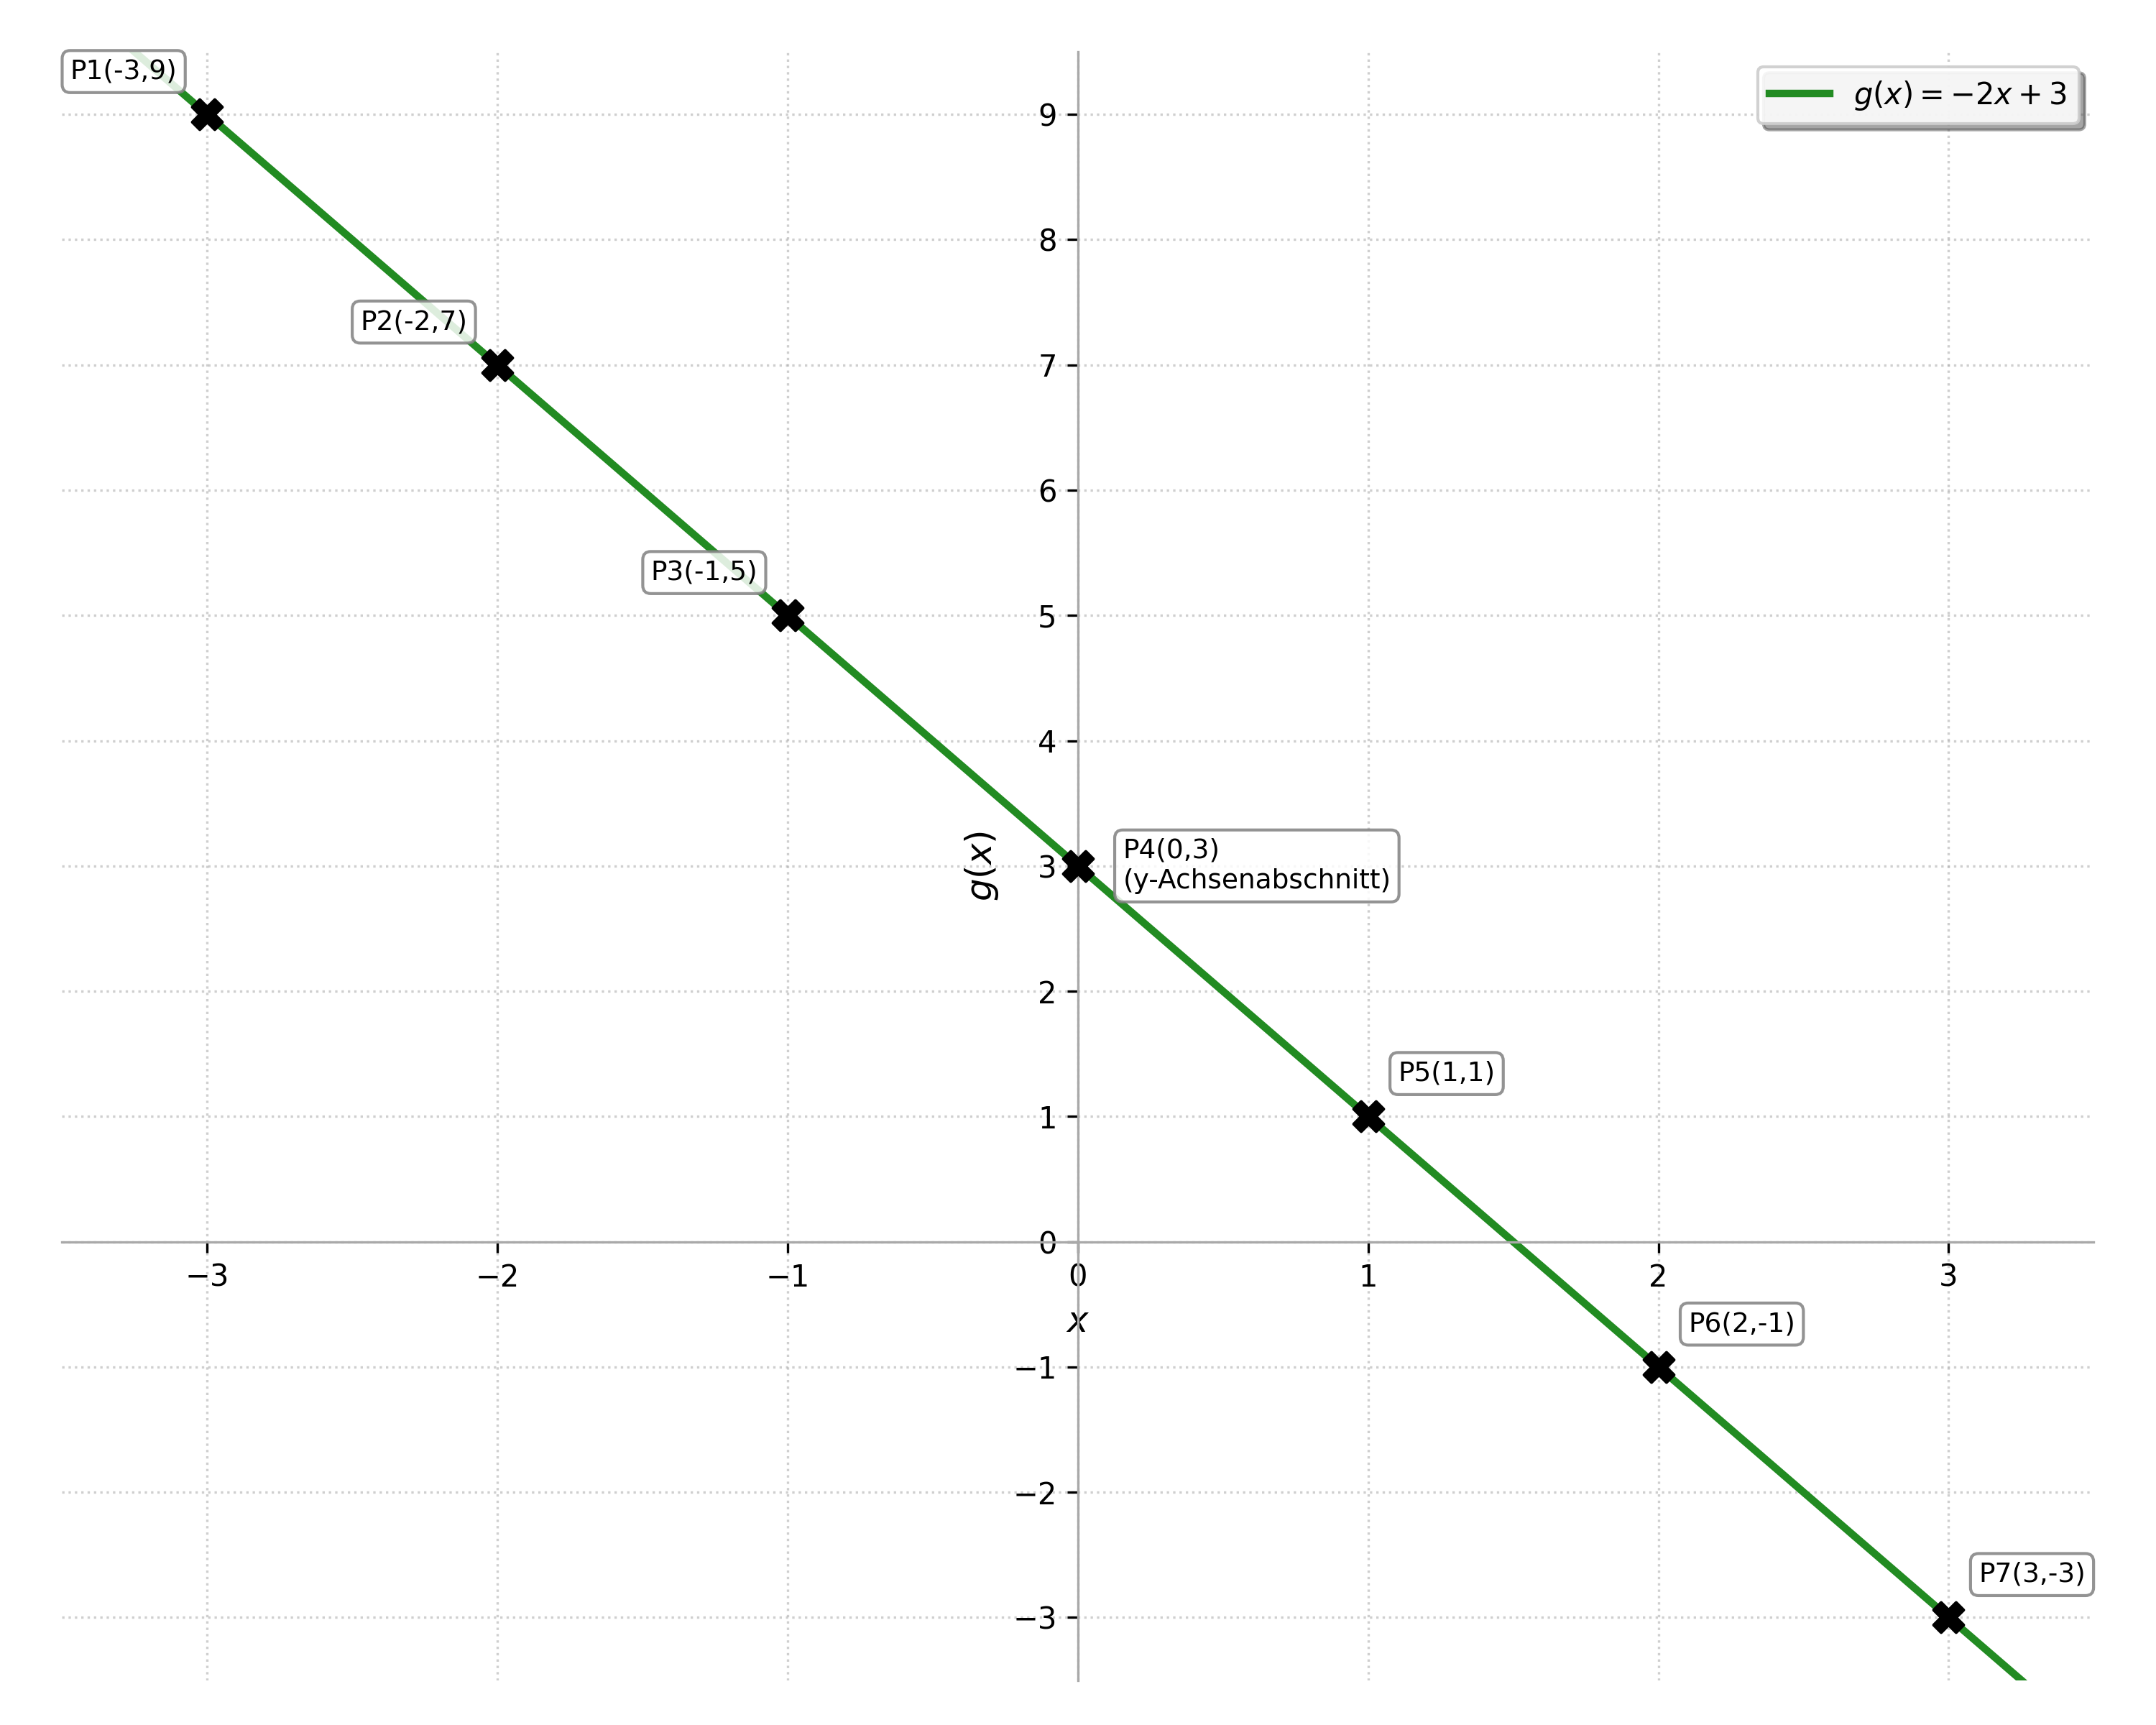
\includegraphics[width=0.8\textwidth]{grafiken/wertetabelle_graph_g_x.png}
% --- Beschreibung der Grafik ---
% Die Grafik sollte ein kartesisches Koordinatensystem zeigen (x-Achse und y-Achse bzw. g(x)-Achse).
% Die x-Achse sollte mindestens von -3 bis 3 skaliert sein.
% Die y-Achse sollte mindestens von -3 bis 9 skaliert sein.
% Die folgenden Punkte aus der Wertetabelle sind deutlich markiert:
% P1(-3|9), P2(-2|7), P3(-1|5), P4(0|3), P5(1|1), P6(2|-1), P7(3|-3).
% Eine Gerade ist durch diese Punkte gezeichnet. Diese Gerade ist der Graph von g(x) = -2x + 3.
% Die Gerade sollte fallend sein, da die Steigung -2 ist.
% Der Schnittpunkt mit der y-Achse bei (0|3) sollte erkennbar sein.
% Die Achsen sind beschriftet.
\captionof{figure}{Graph der Funktion $g(x) = -2x+3$ gezeichnet mit Punkten aus der Wertetabelle.}
\label{fig:graph_g_x}
\end{center}

\begin{tippumgebung}{Graph aus Wertetabelle zeichnen}
Wenn du Punkte aus einer Wertetabelle in ein Koordinatensystem einzeichnest:
\begin{itemize}
    \item Wähle eine passende Skalierung für die x- und y-Achse, damit alle Punkte gut sichtbar sind.
    \item Trage jeden Punkt $(x|y)$ sorgfältig ein: Gehe auf der x-Achse zum x-Wert und von dort parallel zur y-Achse zum y-Wert.
    \item Bei einer linearen Funktion müssen alle Punkte auf einer Geraden liegen. Du kannst ein Lineal verwenden, um dies zu überprüfen und die Gerade zu zeichnen.
    \item Der Punkt $(0|g(0))$ ist immer der Schnittpunkt mit der y-Achse. In diesem Fall $(0|3)$.
\end{itemize}
\end{tippumgebung}

\end{loesungsumgebung}



\begin{aufgabenumgebung}{Umgang mit linearen Funktionen: Werte und Schnittpunkte}

\textbf{Teil 1: Funktion $f(x) = -3x + 7$} \\
Gegeben ist die Funktion $f(x) = -3x + 7$.
\begin{enumerate}[label=(\alph*)]
    \item Berechne $f(-2)$, $f(0)$ und $f(4)$.
    \item Für welchen Wert von $x$ gilt $f(x) = 10$?
    \item Für welchen Wert von $x$ gilt $f(x) = -5$?
    \item An welcher Stelle schneidet der Graph die y-Achse? An welcher die x-Achse (Nullstelle)?
\end{enumerate}

\bigskip % Fügt einen größeren vertikalen Abstand ein

\textbf{Teil 2: Funktion $g(x) = \frac{1}{2}x - 1$} \\
Gegeben ist die Funktion $g(x) = \frac{1}{2}x - 1$.
\begin{enumerate}[label=(\alph*)]
    \item Berechne $g(-4)$, $g(0)$ und $g(6)$.
    \item Für welchen Wert von $x$ gilt $g(x) = 3$?
    \item Für welchen Wert von $x$ gilt $g(x) = -2.5$?
    \item An welcher Stelle schneidet der Graph die y-Achse? An welcher die x-Achse (Nullstelle)?
\end{enumerate}

\bigskip % Fügt einen größeren vertikalen Abstand ein

\textbf{Teil 3: Funktion $h(x) = -4x$} \\
Gegeben ist die Funktion $h(x) = -4x$.
\begin{enumerate}[label=(\alph*)]
    \item Berechne $h(-1.5)$, $h(0)$ und $h(2.5)$.
    \item Für welchen Wert von $x$ gilt $h(x) = 12$?
    \item Für welchen Wert von $x$ gilt $h(x) = -1$?
    \item An welcher Stelle schneidet der Graph die y-Achse? An welcher die x-Achse (Nullstelle)? Was ist hier besonders?
\end{enumerate}
\end{aufgabenumgebung}


\begin{loesungsumgebung}[loes:werte-und-schnittpunkte]{Umgang mit linearen Funktionen: Werte und Schnittpunkte}

\subsection*{Teil 1: Funktion $f(x) = -3x + 7$}
Gegeben ist die Funktion $f(x) = -3x + 7$.

\begin{enumerate}[label=(\alph*)]
    \item \textbf{Berechne $f(-2)$, $f(0)$ und $f(4)$.}
    \begin{itemize}
        \item $f(-2) = -3(-2) + 7 = 6 + 7 = 13$
        \item $f(0) = -3(0) + 7 = 0 + 7 = 7$
        \item $f(4) = -3(4) + 7 = -12 + 7 = -5$
    \end{itemize}

    \item \textbf{Für welchen Wert von $x$ gilt $f(x) = 10$?} \\
    Wir setzen $f(x) = 10$:
    $$
    \begin{array}{r c l c l}
    \umformung{-3x + 7}{10}{-}{7}
    \umformung{-3x}{3}{\div}{(-3)}
    \umformungend{x}{-1}
    \end{array}
    $$
    Für $x=-1$ gilt $f(x)=10$.

    \item \textbf{Für welchen Wert von $x$ gilt $f(x) = -5$?} \\
    Wir setzen $f(x) = -5$:
    $$
    \begin{array}{r c l c l}
    \umformung{-3x + 7}{-5}{-}{7}
    \umformung{-3x}{-12}{\div}{(-3)}
    \umformungend{x}{4}
    \end{array}
    $$
    Für $x=4$ gilt $f(x)=-5$.

    \item \textbf{An welcher Stelle schneidet der Graph die y-Achse? An welcher die x-Achse (Nullstelle)?}
    \begin{itemize}
        \item \textbf{Schnittpunkt mit der y-Achse:} \\
        Dieser liegt bei $x=0$. Der y-Wert ist $f(0) = -3(0) + 7 = 7$. \\
        Der Graph schneidet die y-Achse im Punkt $S_y(0|7)$.
        \item \textbf{Schnittpunkt mit der x-Achse (Nullstelle):} \\
        Wir setzen $f(x)=0$:
        $$
        \begin{array}{r c l c l}
        \umformung{-3x + 7}{0}{-}{7}
        \umformung{-3x}{-7}{\div}{(-3)}
        \umformungend{x}{\frac{7}{3}}
        \end{array}
        $$
        Die Nullstelle ist $x_N = \frac{7}{3}$. \\
        Der Graph schneidet die x-Achse im Punkt $S_x\left(\frac{7}{3}|0\right)$.
    \end{itemize}
\end{enumerate}

\bigskip % Fügt einen größeren vertikalen Abstand ein

\subsection*{Teil 2: Funktion $g(x) = \frac{1}{2}x - 1$}
Gegeben ist die Funktion $g(x) = \frac{1}{2}x - 1$.

\begin{enumerate}[label=(\alph*)]
    \item \textbf{Berechne $g(-4)$, $g(0)$ und $g(6)$.}
    \begin{itemize}
        \item $g(-4) = \frac{1}{2}(-4) - 1 = -2 - 1 = -3$
        \item $g(0) = \frac{1}{2}(0) - 1 = 0 - 1 = -1$
        \item $g(6) = \frac{1}{2}(6) - 1 = 3 - 1 = 2$
    \end{itemize}

    \item \textbf{Für welchen Wert von $x$ gilt $g(x) = 3$?} \\
    Wir setzen $g(x)=3$:
    $$
    \begin{array}{r c l c l}
    \umformung{\frac{1}{2}x - 1}{3}{+}{1}
    \umformung{\frac{1}{2}x}{4}{\cdot}{2}
    \umformungend{x}{8}
    \end{array}
    $$
    Für $x=8$ gilt $g(x)=3$.

    \item \textbf{Für welchen Wert von $x$ gilt $g(x) = -2.5$?} \\
    Wir setzen $g(x)=-2.5$:
    $$
    \begin{array}{r c l c l}
    \umformung{\frac{1}{2}x - 1}{-2.5}{+}{1}
    \umformung{\frac{1}{2}x}{-1.5}{\cdot}{2}
    \umformungend{x}{-3}
    \end{array}
    $$
    Für $x=-3$ gilt $g(x)=-2.5$.

    \item \textbf{An welcher Stelle schneidet der Graph die y-Achse? An welcher die x-Achse (Nullstelle)?}
    \begin{itemize}
        \item \textbf{Schnittpunkt mit der y-Achse:} \\
        Dieser liegt bei $x=0$. Der y-Wert ist $g(0) = \frac{1}{2}(0) - 1 = -1$. \\
        Der Graph schneidet die y-Achse im Punkt $S_y(0|-1)$.
        \item \textbf{Schnittpunkt mit der x-Achse (Nullstelle):} \\
        Wir setzen $g(x)=0$:
        $$
        \begin{array}{r c l c l}
        \umformung{\frac{1}{2}x - 1}{0}{+}{1}
        \umformung{\frac{1}{2}x}{1}{\cdot}{2}
        \umformungend{x}{2}
        \end{array}
        $$
        Die Nullstelle ist $x_N = 2$. \\
        Der Graph schneidet die x-Achse im Punkt $S_x(2|0)$.
    \end{itemize}
\end{enumerate}

\bigskip % Fügt einen größeren vertikalen Abstand ein

\subsection*{Teil 3: Funktion $h(x) = -4x$}
Gegeben ist die Funktion $h(x) = -4x$.

\begin{enumerate}[label=(\alph*)]
    \item \textbf{Berechne $h(-1.5)$, $h(0)$ und $h(2.5)$.}
    \begin{itemize}
        \item $h(-1.5) = -4(-1.5) = 6$
        \item $h(0) = -4(0) = 0$
        \item $h(2.5) = -4(2.5) = -10$
    \end{itemize}

    \item \textbf{Für welchen Wert von $x$ gilt $h(x) = 12$?} \\
    Wir setzen $h(x)=12$:
    $$
    \begin{array}{r c l c l}
    \umformung{-4x}{12}{\div}{(-4)}
    \umformungend{x}{-3}
    \end{array}
    $$
    Für $x=-3$ gilt $h(x)=12$.

    \item \textbf{Für welchen Wert von $x$ gilt $h(x) = -1$?} \\
    Wir setzen $h(x)=-1$:
    $$
    \begin{array}{r c l c l}
    \umformung{-4x}{-1}{\div}{(-4)}
    \umformungend{x}{\frac{1}{4}} % oder 0.25
    \end{array}
    $$
    Für $x=\frac{1}{4}$ (oder $x=0.25$) gilt $h(x)=-1$.

    \item \textbf{An welcher Stelle schneidet der Graph die y-Achse? An welcher die x-Achse (Nullstelle)? Was ist hier besonders?}
    \begin{itemize}
        \item \textbf{Schnittpunkt mit der y-Achse:} \\
        Dieser liegt bei $x=0$. Der y-Wert ist $h(0) = -4(0) = 0$. \\
        Der Graph schneidet die y-Achse im Punkt $S_y(0|0)$.
        \item \textbf{Schnittpunkt mit der x-Achse (Nullstelle):} \\
        Wir setzen $h(x)=0$:
        $$
        \begin{array}{r c l c l}
        \umformung{-4x}{0}{\div}{(-4)}
        \umformungend{x}{0}
        \end{array}
        $$
        Die Nullstelle ist $x_N = 0$. \\
        Der Graph schneidet die x-Achse im Punkt $S_x(0|0)$.
        \item \textbf{Was ist hier besonders?} \\
        Der Schnittpunkt mit der y-Achse $S_y(0|0)$ und der Schnittpunkt mit der x-Achse $S_x(0|0)$ sind identisch. Beide Schnittpunkte liegen im Ursprung des Koordinatensystems. Dies ist charakteristisch für proportionale Funktionen (lineare Funktionen ohne konstanten Term, d.h. $b=0$), deren Graphen immer durch den Ursprung verlaufen.
    \end{itemize}
\end{enumerate}

\end{loesungsumgebung}



\begin{aufgabenumgebung}{Schnittpunkte berechnen und zeichnen}
\begin{enumerate}
    \item Berechne den Schnittpunkt der folgenden Geradenpaare:
        \begin{itemize}
            \item $f(x) = x + 3$ und $g(x) = -2x + 9$
            \item $h(x) = 0.25x - 2$ und $k(x) = 0.25x + 1$ (Was stellst du hier fest? Wie liegen die Geraden zueinander?)
            \item $m(x) = \frac{1}{3}x + 1$ und $n(x) = -\frac{2}{3}x + 4$
        \end{itemize}
    \item Gegeben sind die Funktionen $f(x) = -x+5$ und $g(x) = 2x-1$.
        \begin{itemize}
            \item Berechne ihren Schnittpunkt $S$.
            \item Zeichne beide Geraden und ihren Schnittpunkt in ein Koordinatensystem.
        \end{itemize}
\end{enumerate}
\end{aufgabenumgebung}


\begin{loesungsumgebung}[loes:schnittpunkte-berechnen-zeichnen]{Schnittpunkte berechnen und zeichnen}

\begin{enumerate}
    \item \textbf{Berechnung der Schnittpunkte von Geradenpaaren:}
    Um den Schnittpunkt zweier Geraden $f(x)$ und $g(x)$ zu finden, setzt man die Funktionsterme gleich ($f(x)=g(x)$) und löst die entstehende Gleichung nach $x$ auf. Den gefundenen $x$-Wert setzt man dann in eine der ursprünglichen Geradengleichungen ein, um den zugehörigen $y$-Wert des Schnittpunktes $S(x|y)$ zu erhalten.

    \begin{itemize}
        \item \textbf{Geraden $f(x) = x + 3$ und $g(x) = -2x + 9$} \\
        Gleichsetzen: $f(x) = g(x)$
        $$ x + 3 = -2x + 9 $$
        Umformungsschritte:
        $$
        \begin{array}{r c l c l}
        \umformung{x+3}{-2x+9}{+}{2x}
        \umformung{3x+3}{9}{-}{3}
        \umformung{3x}{6}{\div}{3}
        \umformungend{x}{2}
        \end{array}
        $$
        Den $x$-Wert in $f(x)$ einsetzen (oder in $g(x)$):
        $f(2) = 2 + 3 = 5$.
        Der Schnittpunkt ist $S(2|5)$.

        \item \textbf{Geraden $h(x) = 0.25x - 2$ und $k(x) = 0.25x + 1$} \\
        Gleichsetzen: $h(x) = k(x)$
        $$ 0.25x - 2 = 0.25x + 1 $$
        Umformungsschritte:
        $$
        \begin{array}{r c l c l}
        \umformung{0.25x - 2}{0.25x + 1}{-}{0.25x}
        \umformungend{-2}{1} % Dies ist ein Widerspruch
        \end{array}
        $$
        \textbf{Was stellst du hier fest? Wie liegen die Geraden zueinander?} \\
        Die Gleichung $-2 = 1$ ist eine falsche Aussage (ein Widerspruch). Das bedeutet, dass es keinen $x$-Wert gibt, für den die beiden Funktionswerte gleich sind. Die Geraden haben keinen Schnittpunkt.
        Betrachtet man die Funktionsgleichungen, so stellt man fest, dass beide Geraden die gleiche Steigung $m=0.25$ haben, aber unterschiedliche y-Achsenabschnitte ($b_h = -2$ und $b_k = 1$). Geraden mit gleicher Steigung und unterschiedlichem y-Achsenabschnitt sind \textbf{parallel und verschieden (echt parallel)}. Sie schneiden sich daher nie.

        \item \textbf{Geraden $m(x) = \frac{1}{3}x + 1$ und $n(x) = -\frac{2}{3}x + 4$} \\
        Gleichsetzen: $m(x) = n(x)$
        $$ \frac{1}{3}x + 1 = -\frac{2}{3}x + 4 $$
        Umformungsschritte:
        $$
        \begin{array}{r c l c l}
        \umformung{\frac{1}{3}x + 1}{-\frac{2}{3}x + 4}{+}{\frac{2}{3}x}
        \umformung{x + 1}{4}{-}{1}
        \umformungend{x}{3}
        \end{array}
        $$
        Den $x$-Wert in $m(x)$ einsetzen (oder in $n(x)$):
        $m(3) = \frac{1}{3}(3) + 1 = 1 + 1 = 2$.
        Der Schnittpunkt ist $S(3|2)$.
    \end{itemize}

    \item \textbf{Gegeben sind die Funktionen $f(x) = -x+5$ und $g(x) = 2x-1$.}
    \begin{itemize}
        \item \textbf{Berechne ihren Schnittpunkt $S$.} \\
        Gleichsetzen: $f(x) = g(x)$
        $$ -x + 5 = 2x - 1 $$
        Umformungsschritte:
        $$
        \begin{array}{r c l c l}
        \umformung{-x+5}{2x-1}{-}{2x}
        \umformung{-3x+5}{-1}{-}{5}
        \umformung{-3x}{-6}{\div}{(-3)}
        \umformungend{x}{2}
        \end{array}
        $$
        Den $x$-Wert in $f(x)$ einsetzen (oder in $g(x)$):
        $f(2) = -(2) + 5 = -2 + 5 = 3$.
        Der Schnittpunkt ist $S(2|3)$.

        \item \textbf{Zeichne beide Geraden und ihren Schnittpunkt in ein Koordinatensystem.}
        \begin{center}
        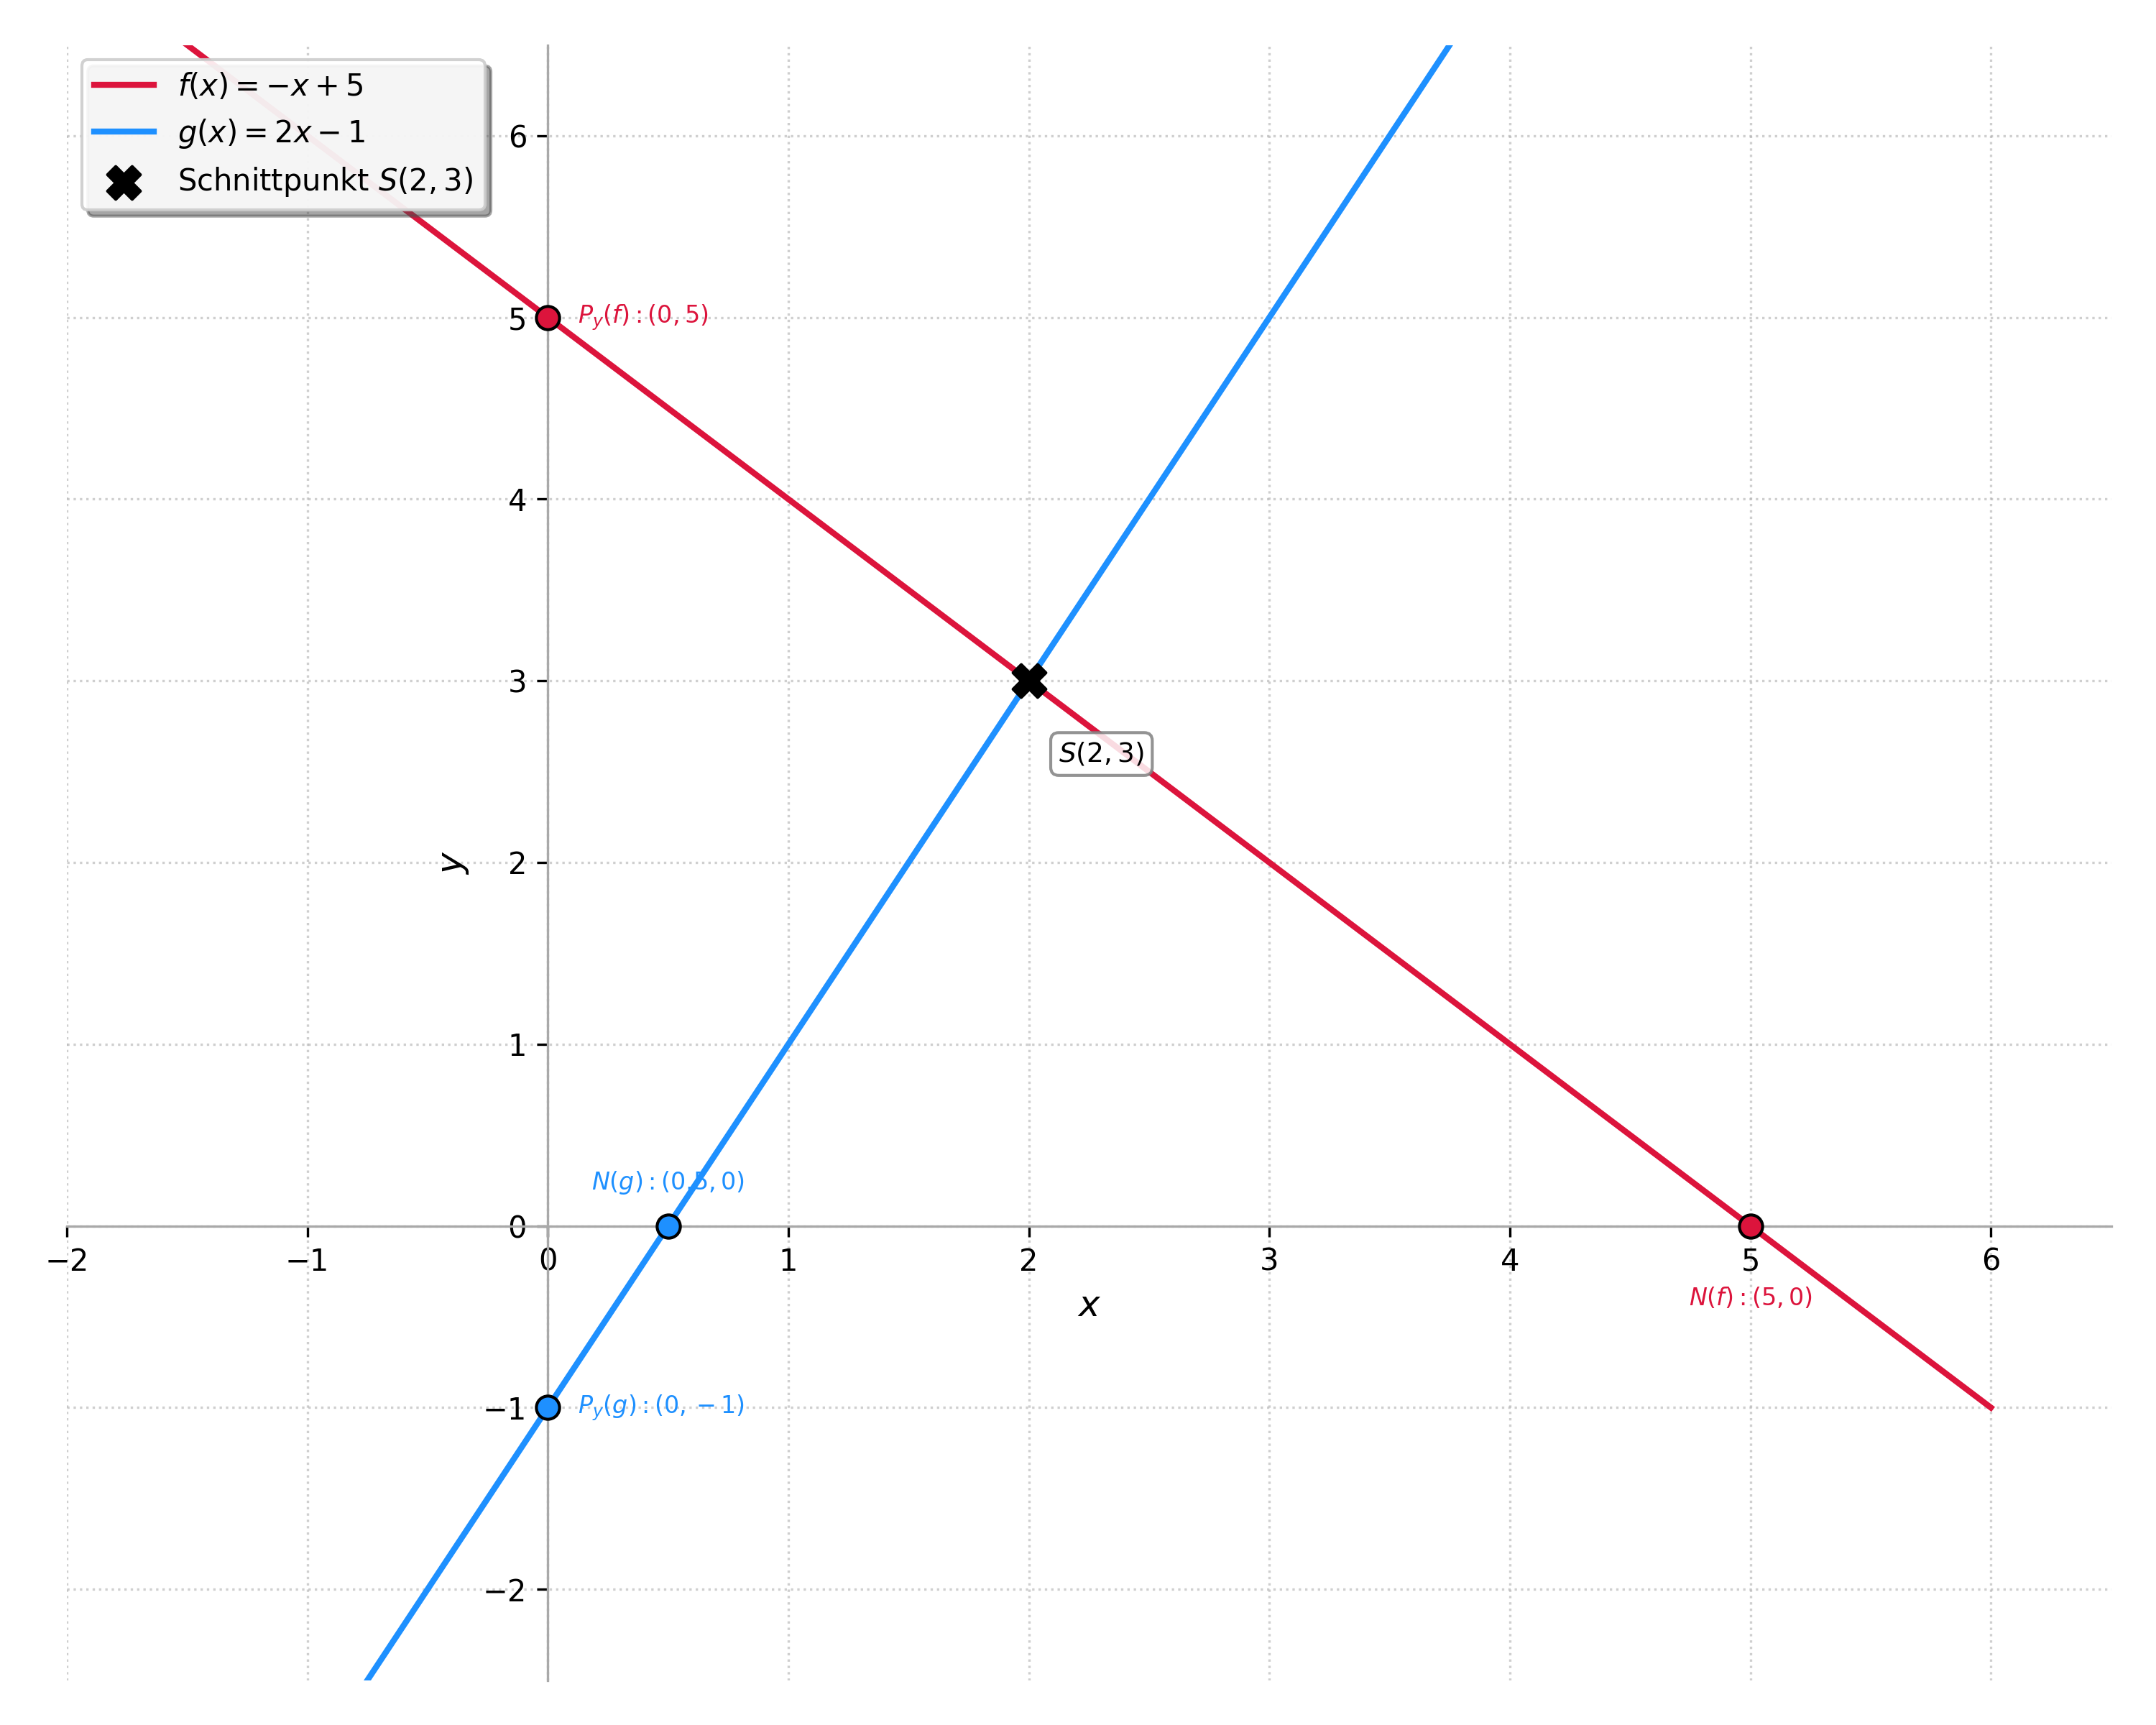
\includegraphics[width=0.8\textwidth]{grafiken/schnittpunkt_teil2_f_g.png}
        % --- Beschreibung der Grafik ---
        % Die Grafik sollte ein kartesisches Koordinatensystem zeigen.
        % Die x-Achse und y-Achse sind beschriftet und sinnvoll skaliert (z.B. von -2 bis 6 für x und -2 bis 6 für y).
        % Eingezeichnet sind die beiden Geraden:
        % 1. f(x) = -x + 5: y-Achsenabschnitt bei (0|5), Nullstelle bei (5|0). Die Gerade fällt.
        % 2. g(x) = 2x - 1: y-Achsenabschnitt bei (0|-1), Nullstelle bei (0.5|0). Die Gerade steigt.
        % Der berechnete Schnittpunkt S(2|3) ist deutlich markiert und liegt auf beiden Geraden.
        % Die Geraden könnten zur besseren Unterscheidung farblich oder durch Beschriftung (f(x), g(x)) gekennzeichnet sein.
        \captionof{figure}{Graphische Darstellung der Geraden $f(x) = -x+5$ und $g(x) = 2x-1$ mit ihrem Schnittpunkt $S(2|3)$.}
        \label{fig:schnittpunkt_f_g_teil2}
        \end{center}
    \end{itemize}
\end{enumerate}

\end{loesungsumgebung}

\begin{aufgabenumgebung}{Taxifahrt}
Ein Taxifahrer verlangt eine Grundgebühr von 3,50 Euro für jede Fahrt. Zusätzlich kostet jeder gefahrene Kilometer 2 Euro.
\begin{enumerate}
    \item Stelle die Kostenfunktion $K(x)$ auf, wobei $x$ die Anzahl der gefahrenen Kilometer ist. Identifiziere $a$ und $b$ und erkläre ihre Bedeutung in diesem Kontext.
    \item Wie viel kostet eine Fahrt von 15 km?
    \item Du hast 25 Euro dabei. Wie viele Kilometer kannst du maximal fahren, wenn du den vollen Betrag ausgeben möchtest? (Tipp: Setze $K(x)=25$ und löse die Gleichung nach $x$ auf.)
    \item Zeichne den Graphen der Funktion $K(x)$ für $x$-Werte von 0 km bis 20 km. Wähle passende Einheiten für die Achsen.
\end{enumerate}
\end{aufgabenumgebung}


\begin{loesungsumgebung}[loes:taxifahrt]{Taxifahrt}
Die Kosten für eine Taxifahrt setzen sich aus einer festen Grundgebühr und einem variablen Preis pro Kilometer zusammen. Dies lässt sich mathematisch durch eine lineare Funktion modellieren.

\begin{enumerate}
    \item \textbf{Kostenfunktion $K(x)$ aufstellen} \\
    Die allgemeine Form einer linearen Funktion ist $f(x) = ax + b$. In diesem Kontext ist:
    \begin{itemize}
        \item $x$: die Anzahl der gefahrenen Kilometer.
        \item $b$: die Grundgebühr, die unabhängig von der Strecke anfällt. Hier beträgt sie 3,50 Euro.
        \item $a$: die Kosten pro gefahrenem Kilometer. Hier sind es 2 Euro pro Kilometer.
    \end{itemize}
    Somit lautet die Kostenfunktion $K(x)$:
    $$ K(x) = 2x + 3.50 $$
    Identifikation und Bedeutung von $a$ und $b$:
    \begin{itemize}
        \item $a = 2$ (Euro/km): Dies ist die \textbf{Steigung} der Geraden. Sie gibt an, um wie viel sich die Gesamtkosten erhöhen, wenn ein zusätzlicher Kilometer gefahren wird. Jeder weitere Kilometer kostet also 2 Euro mehr.
        \item $b = 3.50$ (Euro): Dies ist der \textbf{y-Achsenabschnitt} der Geraden. Er repräsentiert die Fixkosten, also die Grundgebühr, die auch dann anfällt, wenn keine Kilometer gefahren werden ($x=0$). Es sind die Kosten für das Antreten der Fahrt.
    \end{itemize}

    \item \textbf{Wie viel kostet eine Fahrt von 15 km?} \\
    Wir setzen $x=15$ in die Kostenfunktion $K(x)$ ein:
    $$ K(15) = 2 \cdot (15) + 3.50 $$
    $$ K(15) = 30 + 3.50 $$
    $$ K(15) = 33.50 $$
    Eine Fahrt von 15 km kostet 33,50 Euro.

    \item \textbf{Wie viele Kilometer kannst du maximal fahren, wenn du 25 Euro dabei hast?} \\
    Wir setzen $K(x) = 25$ und lösen die Gleichung nach $x$ auf:
    $$ 2x + 3.50 = 25 $$
    Umformungsschritte:
    $$
    \begin{array}{r c l c l}
    \umformung{2x + 3.50}{25}{-}{3.50}
    \umformung{2x}{21.50}{\div}{2}
    \umformungend{x}{10.75}
    \end{array}
    $$
    Du kannst maximal 10,75 Kilometer fahren.

    \item \textbf{Zeichne den Graphen der Funktion $K(x)$ für $x$-Werte von 0 km bis 20 km.}
    \begin{center}
    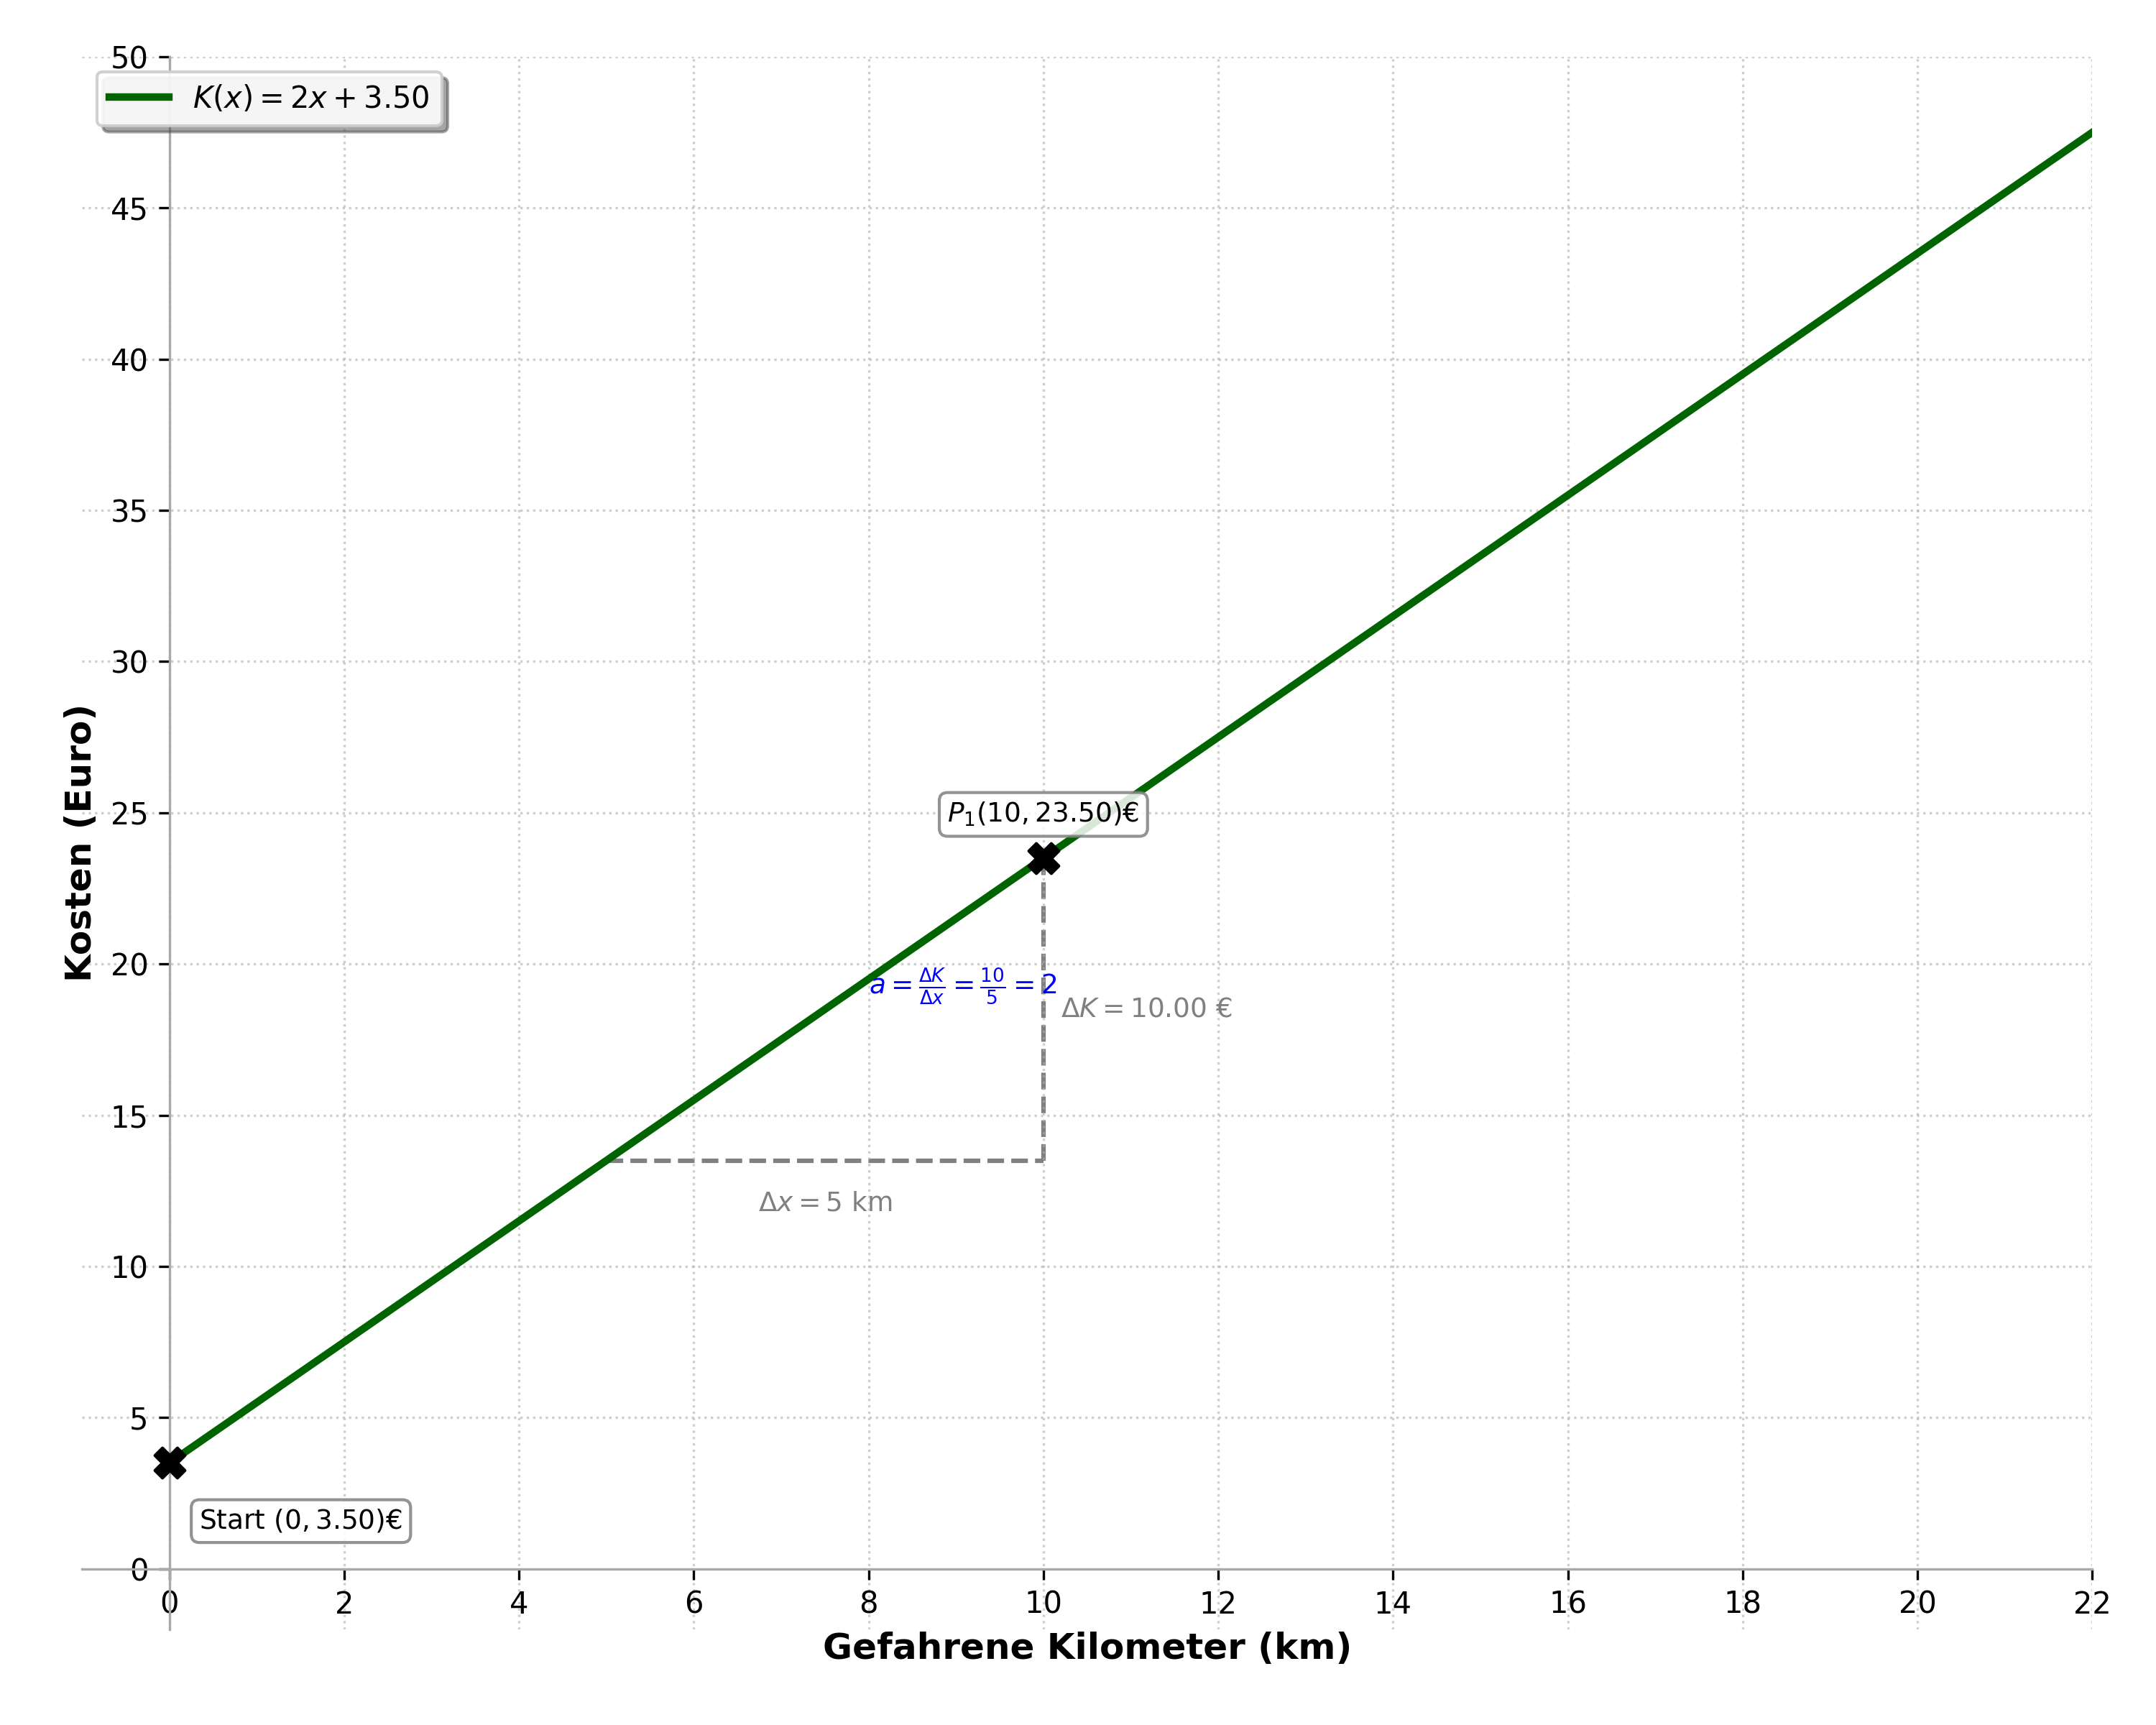
\includegraphics[width=0.8\textwidth]{grafiken/taxikosten_graph.png}
    % --- Beschreibung der Grafik ---
    % Die Grafik sollte ein kartesisches Koordinatensystem zeigen.
    % Die x-Achse ist mit 'Gefahrene Kilometer (km)' beschriftet und reicht von 0 bis mindestens 20 km.
    % Die y-Achse ist mit 'Kosten (Euro)' beschriftet und reicht von 0 bis ca. 45-50 Euro (da K(20) = 2*20 + 3.50 = 43.50 Euro).
    % Der Graph der Funktion K(x) = 2x + 3.50 ist als Gerade eingezeichnet, die bei x=0 beginnt.
    % Wichtige Punkte sind markiert oder ablesbar:
    % - Der y-Achsenabschnitt (Startpunkt der Fahrtkosten) bei (0 | 3.50).
    % - Ein weiterer Punkt, z.B. (10 | 23.50) oder der Endpunkt (20 | 43.50).
    % - Die Steigung von 2 (pro 1 km nach rechts geht es 2 Euro nach oben) sollte aus dem Graphen ersichtlich sein (z.B. durch ein Steigungsdreieck).
    \captionof{figure}{Graph der Kostenfunktion $K(x) = 2x + 3.50$ für eine Taxifahrt.}
    \label{fig:taxikosten}
    \end{center}
    \textbf{Erläuterung zur Zeichnung:}
    Der Graph beginnt auf der y-Achse beim Wert der Grundgebühr (3,50 Euro). Von dort steigt die Gerade linear an. Für jeden Kilometer, den man auf der x-Achse nach rechts geht, steigen die Kosten auf der y-Achse um 2 Euro. Für eine Strecke von 20 km würden die Kosten $K(20) = 2(20) + 3.50 = 43.50$ Euro betragen. Die Achsen sollten so skaliert sein, dass dieser Bereich gut dargestellt wird.
\end{enumerate}

\end{loesungsumgebung}

\begin{aufgabenumgebung}[labelA:LinUeb]{Lineare Funktionen – Übungen querbeet}
\begin{enumerate}
    \item \textbf{Paketversand:} Ein Paketversand kostet 5 Euro Grundgebühr. Jedes Kilogramm Gewicht kostet zusätzlich 1,50 Euro.
        \begin{itemize}
            \item Wie lautet die Kostenfunktion $K(g)$, wenn $g$ das Gewicht in Kilogramm ist?
            \item Was kostet ein Paket, das 3,2 kg wiegt?
            \item Ein Paket kostet 15,50 Euro. Wie schwer war es?
        \end{itemize}
    \item \textbf{Kerzenlänge:} Eine Kerze ist anfangs 20 cm lang. Pro Stunde brennt sie gleichmäßig 2,5 cm ab.
        \begin{itemize}
            \item Stelle eine Funktion $L(t)$ auf, die die Länge der Kerze nach $t$ Stunden beschreibt. (Achtung: Die Länge nimmt ab. Was bedeutet das für das Vorzeichen der Steigung $a$?)
            \item Wie lang ist die Kerze nach 3 Stunden?
            \item Nach wie vielen Stunden ist die Kerze komplett abgebrannt? (Das bedeutet, ihre Länge ist 0 cm.)
            \item Für welchen Zeitraum $t$ ist diese Funktion realistisch? (Definitionsbereich der Anwendung)
        \end{itemize}
    \item \textbf{Funktion aus Punkten:} Eine Gerade geht durch die Punkte $P_1(2|5)$ und $P_2(5|14)$. Bestimme ihre Funktionsgleichung $f(x)=ax+b$.
    \item \textbf{Funktion aus Steigung und Punkt:} Die Steigung einer Geraden ist $a = -2$. Die Gerade geht außerdem durch den Punkt $P(1|3)$. Bestimme den y-Achsenabschnitt $b$ und gib die vollständige Funktionsgleichung an. (Tipp: Setze $a$ und die Koordinaten von $P$ in $y=ax+b$ ein und löse nach $b$.)
\end{enumerate}
\end{aufgabenumgebung}


\begin{loesungsumgebung}[loes:LinUeb]{Lineare Funktionen – Übungen querbeet}

\begin{enumerate}
    \item \textbf{Paketversand:}
    \begin{itemize}
        \item \textbf{Wie lautet die Kostenfunktion $K(g)$, wenn $g$ das Gewicht in Kilogramm ist?} \\
        Die Grundgebühr beträgt 5 Euro (das ist der y-Achsenabschnitt $b$).
        Jedes Kilogramm kostet zusätzlich 1,50 Euro (das ist die Steigung $a$).
        Die Kostenfunktion lautet: $K(g) = 1.50g + 5$.

        \item \textbf{Was kostet ein Paket, das 3,2 kg wiegt?} \\
        Wir setzen $g = 3.2$ in die Funktion $K(g)$ ein:
        $K(3.2) = 1.50 \cdot (3.2) + 5 = 4.80 + 5 = 9.80$. \\
        Ein Paket, das 3,2 kg wiegt, kostet 9,80 Euro.

        \item \textbf{Ein Paket kostet 15,50 Euro. Wie schwer war es?} \\
        Wir setzen $K(g) = 15.50$ und lösen nach $g$ auf:
        $$ 1.50g + 5 = 15.50 $$
        Umformungsschritte:
        $$
        \begin{array}{r c l c l}
        \umformung{1.50g + 5}{15.50}{-}{5}
        \umformung{1.50g}{10.50}{\div}{1.50}
        \umformungend{g}{7}
        \end{array}
        $$
        Das Paket war 7 kg schwer.
    \end{itemize}

    \item \textbf{Kerzenlänge:}
    \begin{itemize}
        \item \textbf{Stelle eine Funktion $L(t)$ auf, die die Länge der Kerze nach $t$ Stunden beschreibt.} \\
        Die Anfangslänge beträgt 20 cm (das ist der y-Achsenabschnitt $b$).
        Pro Stunde brennt sie 2,5 cm ab. Da die Länge abnimmt, ist die Steigung $a$ negativ: $a = -2.5$ cm/Stunde.
        Die Funktion für die Länge $L(t)$ nach $t$ Stunden lautet: $L(t) = -2.5t + 20$.

        \item \textbf{Wie lang ist die Kerze nach 3 Stunden?} \\
        Wir setzen $t = 3$ in die Funktion $L(t)$ ein:
        $L(3) = -2.5 \cdot (3) + 20 = -7.5 + 20 = 12.5$. \\
        Nach 3 Stunden ist die Kerze noch 12,5 cm lang.

        \item \textbf{Nach wie vielen Stunden ist die Kerze komplett abgebrannt? (Länge ist 0 cm)} \\
        Wir setzen $L(t) = 0$ und lösen nach $t$ auf:
        $$ -2.5t + 20 = 0 $$
        Umformungsschritte:
        $$
        \begin{array}{r c l c l}
        \umformung{-2.5t + 20}{0}{-}{20}
        \umformung{-2.5t}{-20}{\div}{(-2.5)}
        \umformungend{t}{8}
        \end{array}
        $$
        Die Kerze ist nach 8 Stunden komplett abgebrannt.

        \item \textbf{Für welchen Zeitraum $t$ ist diese Funktion realistisch? (Definitionsbereich der Anwendung)} \\
        Die Zeit $t$ kann nicht negativ sein, also $t \ge 0$. Die Kerze kann nicht weiterbrennen, nachdem sie vollständig abgebrannt ist (nach 8 Stunden). Eine negative Länge ist nicht möglich.
        Daher ist der realistische Definitionsbereich für $t$ (in Stunden): $0 \le t \le 8$.
    \end{itemize}

    \item \textbf{Funktion aus Punkten:} Eine Gerade geht durch die Punkte $P_1(2|5)$ und $P_2(5|14)$. Bestimme ihre Funktionsgleichung $f(x)=ax+b$. \\
    \textbf{Schritt 1: Steigung $a$ berechnen}
    $$ a = \frac{y_2 - y_1}{x_2 - x_1} = \frac{14 - 5}{5 - 2} = \frac{9}{3} = 3 $$
    Die Steigung ist $a=3$.
    \textbf{Schritt 2: y-Achsenabschnitt $b$ berechnen}
    Wir verwenden die Form $f(x) = ax+b$, setzen $a=3$ und die Koordinaten eines Punktes (z.B. $P_1(2|5)$) ein: $x=2, y=5$.
    $$ 5 = 3 \cdot (2) + b $$
    $$ 5 = 6 + b $$
    Umformungsschritte (um $b$ zu isolieren, stellen wir $6+b=5$ um):
    $$
    \begin{array}{r c l c l}
    \umformung{6+b}{5}{-}{6}
    \umformungend{b}{-1}
    \end{array}
    $$
    Der y-Achsenabschnitt ist $b=-1$.
    \textbf{Schritt 3: Funktionsgleichung aufstellen}
    Die Funktionsgleichung lautet $f(x) = 3x - 1$.

    \item \textbf{Funktion aus Steigung und Punkt:} Die Steigung einer Geraden ist $a = -2$. Die Gerade geht außerdem durch den Punkt $P(1|3)$. Bestimme den y-Achsenabschnitt $b$ und gib die vollständige Funktionsgleichung an. \\
    Die allgemeine Form ist $y = ax+b$. Gegeben sind $a=-2$ und der Punkt $P(1|3)$, also $x=1$ und $y=3$.
    \textbf{Schritt 1: y-Achsenabschnitt $b$ berechnen}
    Wir setzen die gegebenen Werte in die Gleichung ein:
    $$ 3 = (-2) \cdot (1) + b $$
    $$ 3 = -2 + b $$
    Umformungsschritte (um $b$ zu isolieren, stellen wir $-2+b=3$ um):
    $$
    \begin{array}{r c l c l}
    \umformung{-2+b}{3}{+}{2}
    \umformungend{b}{5}
    \end{array}
    $$
    Der y-Achsenabschnitt ist $b=5$.
    \textbf{Schritt 2: Vollständige Funktionsgleichung angeben}
    Die Funktionsgleichung lautet $f(x) = -2x + 5$.
\end{enumerate}

\end{loesungsumgebung}

\begin{aufgabenumgebung}{Deine durchschnittliche Rate}
Denke dir ein eigenes Beispiel aus dem Alltag aus, bei dem eine Größe sich über die Zeit oder eine andere Einheit verändert (z.B. Wasserverbrauch einer Familie über mehrere Tage, Wachstum einer Pflanze über Wochen, Temperaturänderung im Laufe eines Tages, Anzahl der gelesenen Seiten eines Buches über mehrere Abende).
\begin{enumerate}
    \item Beschreibe die Situation klar. Welche Größe ändert sich in Abhängigkeit von welcher anderen Größe?
    \item Lege zwei Messpunkte (Anfangswert mit zugehörigem 'x1' und Endwert mit zugehörigem 'x2') fest.
    \item Berechne die durchschnittliche Änderungsrate. Was sagt diese Rate in deinem Beispiel konkret aus? Welche Einheit hat sie?
\end{enumerate}
\end{aufgabenumgebung}

\begin{loesungsumgebung}[loes:durchschnittliche-rate-beispiel]{Deine durchschnittliche Rate}
Hier ist ein Beispiel aus dem Alltag, das eine durchschnittliche Änderungsrate veranschaulicht:

\begin{enumerate}
    \item \textbf{Beschreibung der Situation:} \\
    Wir betrachten das \textbf{Wachstum eines Sonnenblumenkeimlings}.
    Die sich ändernde Größe ist die \textbf{Höhe des Keimlings} (gemessen in Zentimetern, cm).
    Diese Höhe ändert sich in Abhängigkeit von der \textbf{vergangenen Zeit} seit der Keimung (gemessen in Tagen).

    \item \textbf{Zwei Messpunkte festlegen:}
    \begin{itemize}
        \item \textbf{Anfangswert ($x_1, y_1$):} 3 Tage nach der Keimung ($x_1 = 3$ Tage) hat der Sonnenblumenkeimling eine Höhe von $y_1 = 5$ cm erreicht.
        \item \textbf{Endwert ($x_2, y_2$):} 10 Tage nach der Keimung ($x_2 = 10$ Tage) wird die Höhe des Keimlings erneut gemessen und beträgt nun $y_2 = 19$ cm.
    \end{itemize}
    Unsere Messpunkte sind also $P_1(3 \text{ Tage} | 5 \text{ cm})$ und $P_2(10 \text{ Tage} | 19 \text{ cm})$.

    \item \textbf{Berechnung der durchschnittlichen Änderungsrate:} \\
    Die durchschnittliche Änderungsrate $m$ berechnet sich aus der Formel:
    $$ m = \frac{\text{Änderung der Höhe}}{\text{Änderung der Zeit}} = \frac{y_2 - y_1}{x_2 - x_1} $$
    Einsetzen der Werte:
    $$ m = \frac{19 \text{ cm} - 5 \text{ cm}}{10 \text{ Tage} - 3 \text{ Tage}} $$
    $$ m = \frac{14 \text{ cm}}{7 \text{ Tage}} $$
    $$ m = 2 \text{ cm/Tag} $$
    \textbf{Was sagt diese Rate in deinem Beispiel konkret aus?} \\
    Die durchschnittliche Änderungsrate von 2 cm/Tag bedeutet, dass der Sonnenblumenkeimling im Zeitraum zwischen dem 3. und dem 10. Tag nach der Keimung \textbf{durchschnittlich um 2 Zentimeter pro Tag gewachsen ist}. Es ist wichtig zu verstehen, dass dies ein Durchschnittswert ist; an manchen Tagen mag der Keimling etwas mehr oder weniger als 2 cm gewachsen sein.
    \textbf{Welche Einheit hat sie?} \\
    Die Einheit der durchschnittlichen Änderungsrate ist \textbf{Zentimeter pro Tag} (cm/Tag).
\end{enumerate}

\begin{tippumgebung}{Verständnis der durchschnittlichen Änderungsrate}
Die durchschnittliche Änderungsrate ist im Wesentlichen die Steigung der Geraden, die die beiden Messpunkte verbindet (Sekantensteigung). Sie gibt an, wie stark sich eine Größe im Durchschnitt pro Einheit einer anderen Größe ändert. Das Vorzeichen der Rate zeigt an, ob es sich um eine Zunahme (positiv) oder eine Abnahme (negativ) handelt.
\end{tippumgebung}

\end{loesungsumgebung}

\begin{aufgabenumgebung}{Checkliste: Eigenschaften einer linearen Funktion analysieren}
Betrachte die lineare Funktion $f(x) = \frac{1}{2}x - 1$.
Bearbeite die folgenden Punkte, um dein Verständnis dieser Funktion zu überprüfen:

\begin{enumerate}[label=(\alph*)]
    \item \textbf{Nullstelle:} Berechne die Nullstelle $x_0$ der Funktion $f(x)$ (d.h. die Stelle, an der $f(x_0)=0$ ist).
    \item \textbf{Y-Achsenabschnitt:} Bestimme den Schnittpunkt mit der y-Achse (den y-Achsenabschnitt $b$). Welchen Wert hat die Funktion an der Stelle $x=0$?
    \item \textbf{Skizze:} Zeichne den Graphen der Funktion $f(x)$ sorgfältig in ein Koordinatensystem. Markiere deutlich die Nullstelle auf der x-Achse und den y-Achsenabschnitt auf der y-Achse.
    \item \textbf{Funktionswerte positiv/negativ:}
    \begin{itemize}
        \item Für welche $x$-Werte sind die Funktionswerte $f(x)$ \textbf{positiv} (d.h. der Graph verläuft oberhalb der x-Achse)? Gib den Bereich an.
        \item Für welche $x$-Werte sind die Funktionswerte $f(x)$ \textbf{negativ} (d.h. der Graph verläuft unterhalb der x-Achse)? Gib den Bereich an.
    \end{itemize}
    \item \textbf{Rolle der Steigung:} Wie hilft dir das Vorzeichen der Steigung $a = \frac{1}{2}$ dabei, die Bereiche aus Teil (d) schnell zu bestimmen, sobald du die Nullstelle kennst? Erkläre in eigenen Worten.
    \item \textbf{Rolle des y-Achsenabschnitts:} Betrachte den y-Achsenabschnitt $b=-1$. Hilft dir dieser Wert auch dabei, das Vorzeichen der Funktion in einem bestimmten Bereich (z.B. für $x$-Werte nahe Null) zu bestimmen? Begründe.
    \item \textbf{Wertebereich:} Der Wertebereich einer nicht-konstanten linearen Funktion ist die Menge aller reellen Zahlen $\mathbb{R}$. Wie kannst du das an deinem Graphen erkennen oder dir vorstellen, dass jeder y-Wert irgendwann einmal getroffen wird?
\end{enumerate}
\end{aufgabenumgebung}

\begin{loesungsumgebung}[loes:checkliste-lineare-funktion]{Checkliste: Eigenschaften einer linearen Funktion analysieren}
Wir analysieren die lineare Funktion $f(x) = \frac{1}{2}x - 1$.

\begin{enumerate}[label=(\alph*)]
    \item \textbf{Nullstelle:}
    Die Nullstelle $x_0$ ist die Stelle, an der $f(x_0)=0$ ist.
    $$ \frac{1}{2}x_0 - 1 = 0 $$
    Umformungsschritte:
    $$
    \begin{array}{r c l c l}
    \umformung{\frac{1}{2}x_0 - 1}{0}{+}{1}
    \umformung{\frac{1}{2}x_0}{1}{\cdot}{2}
    \umformungend{x_0}{2}
    \end{array}
    $$
    Die Nullstelle ist $x_0 = 2$.

    \item \textbf{Y-Achsenabschnitt:}
    Der y-Achsenabschnitt $b$ ist der konstante Term in der Funktionsgleichung $f(x) = ax+b$. Für $f(x) = \frac{1}{2}x - 1$ ist $b = -1$.
    Der Schnittpunkt mit der y-Achse ist der Punkt $S_y(0|b)$, also $S_y(0|-1)$.
    Der Wert der Funktion an der Stelle $x=0$ ist $f(0) = \frac{1}{2}(0) - 1 = -1$. Dies bestätigt den y-Achsenabschnitt.

    \item \textbf{Skizze:}
    \begin{center}
    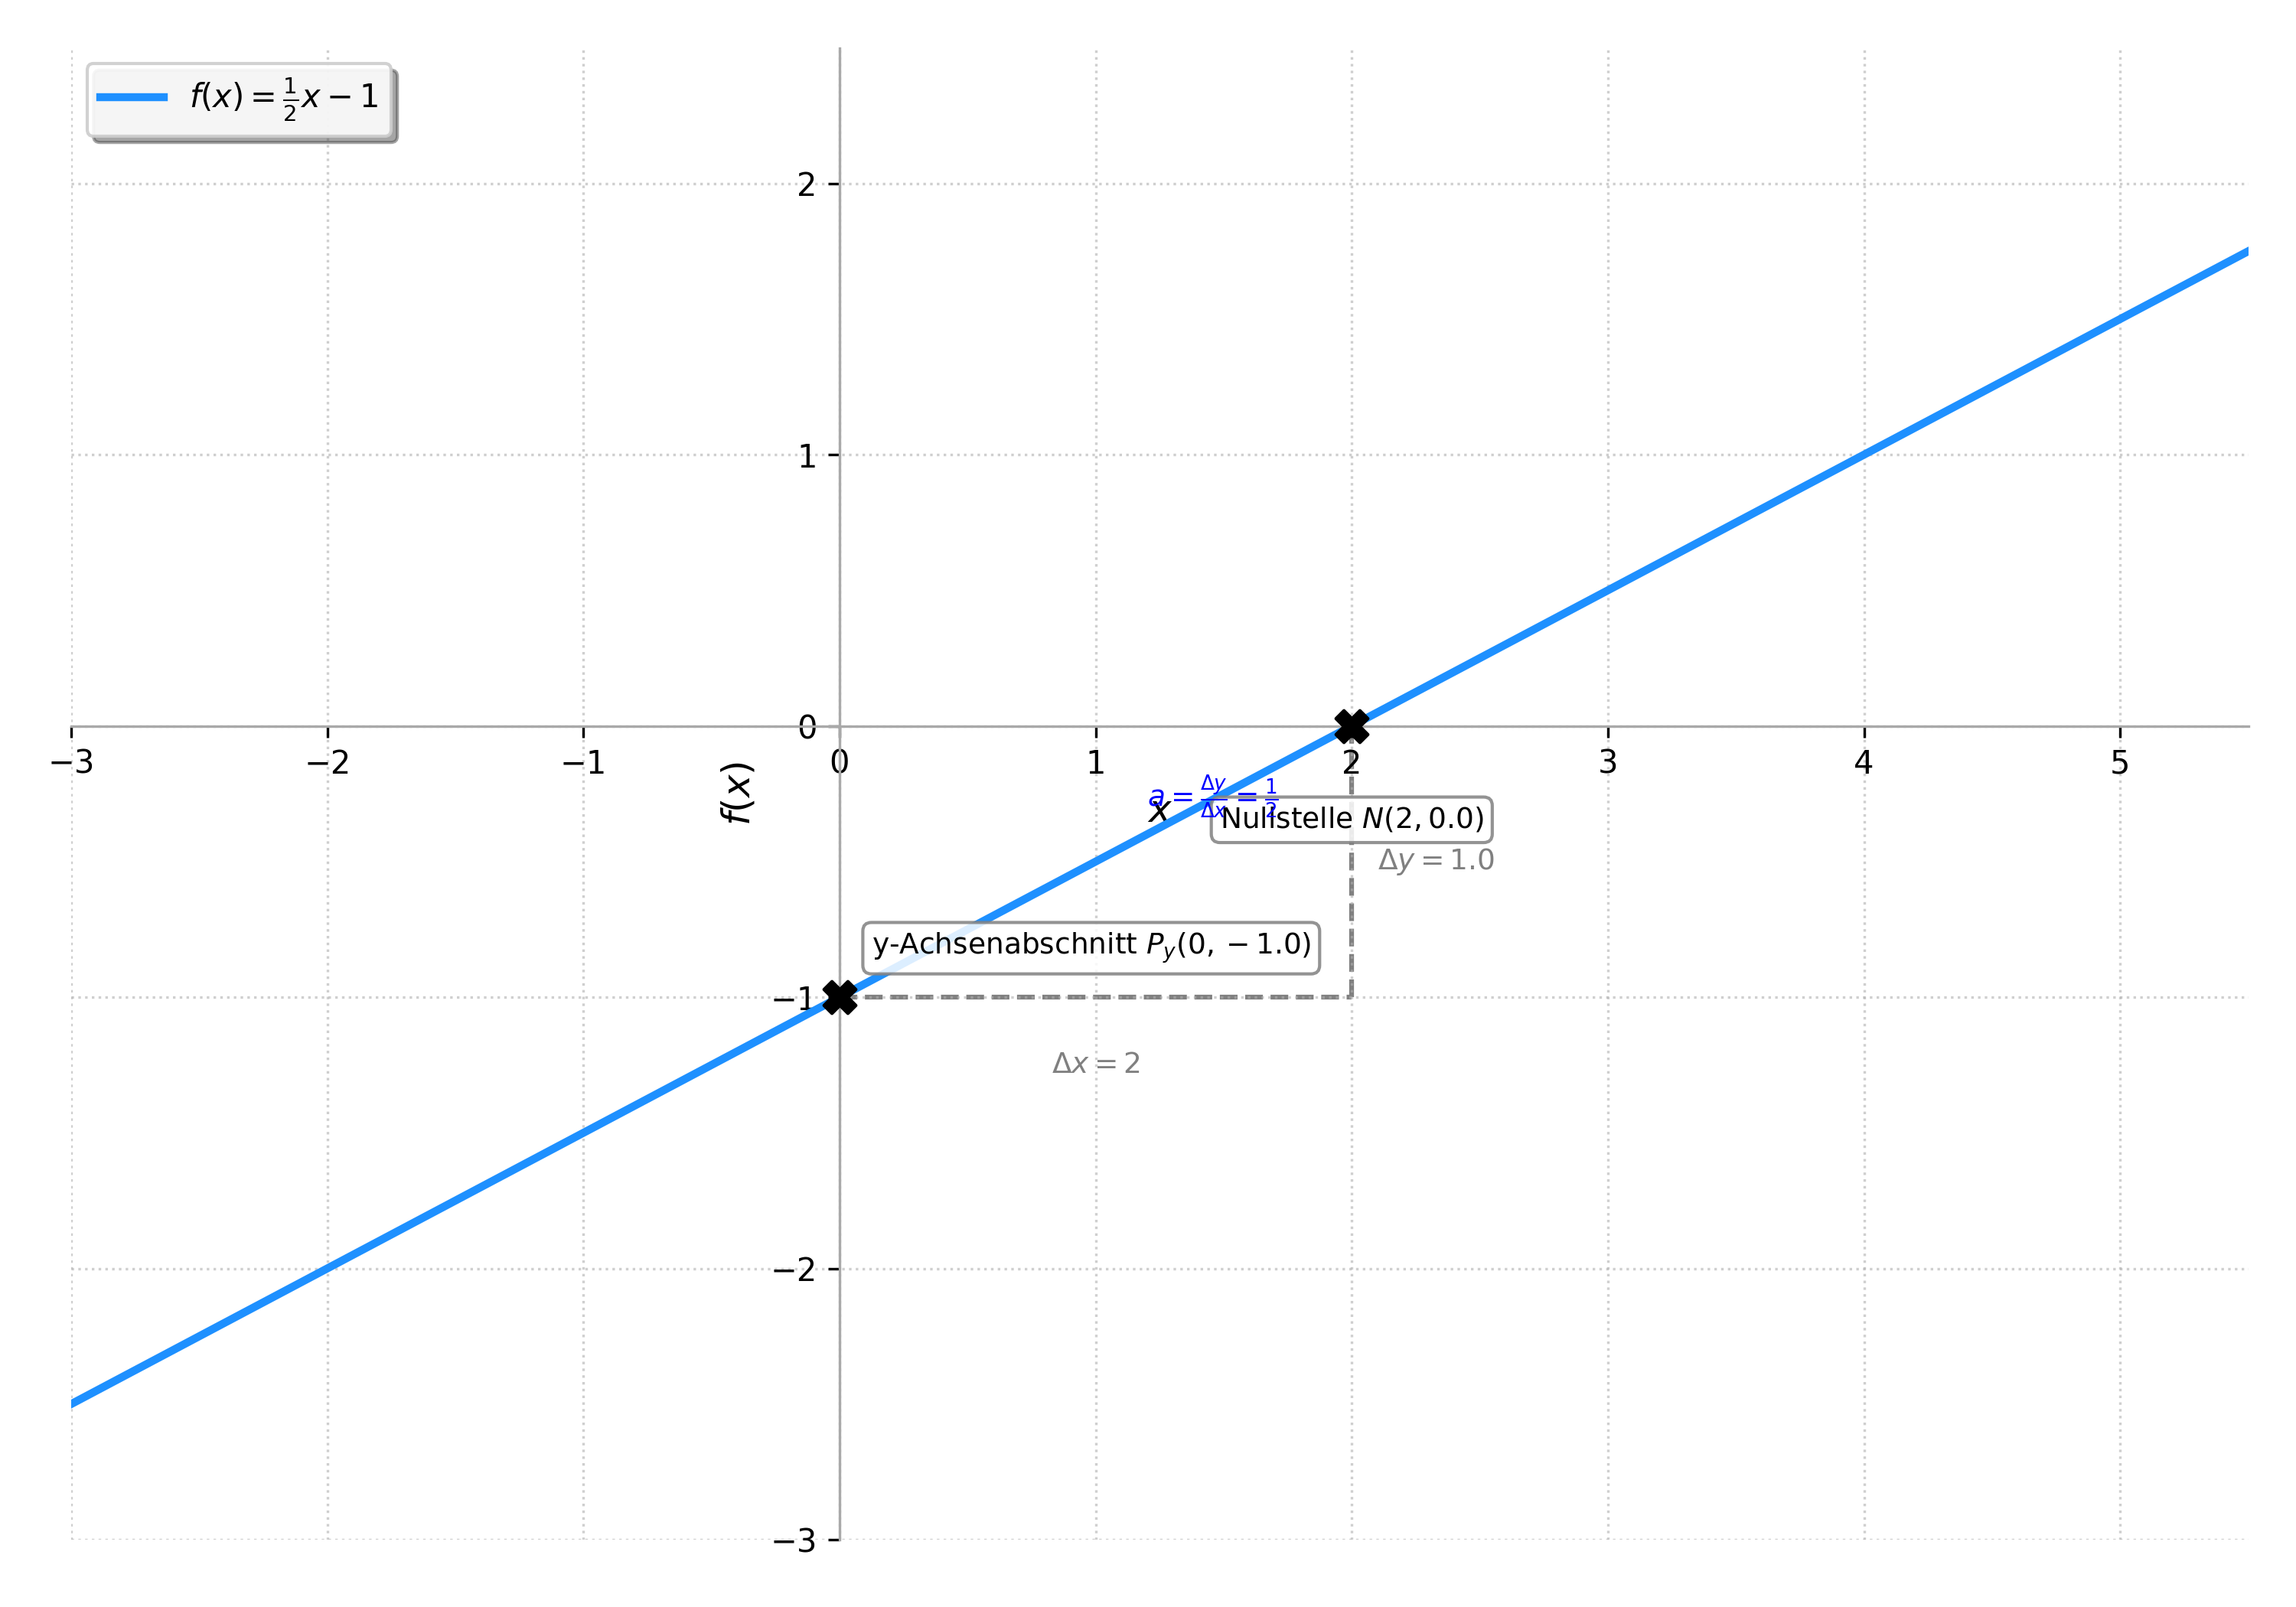
\includegraphics[width=0.8\textwidth]{grafiken/funktion_checkliste_graph.png}
    % --- Beschreibung der Grafik ---
    % Die Grafik zeigt ein kartesisches Koordinatensystem.
    % Die x-Achse und y-Achse sind beschriftet und sinnvoll skaliert (z.B. von -3 bis 5 für x und -3 bis 2 für y).
    % Eingezeichnet ist der Graph der Funktion f(x) = (1/2)x - 1. Es ist eine Gerade.
    % Die Nullstelle (Schnittpunkt mit der x-Achse) bei (2|0) ist deutlich markiert.
    % Der y-Achsenabschnitt (Schnittpunkt mit der y-Achse) bei (0|-1) ist deutlich markiert.
    % Die Gerade steigt an, was der positiven Steigung a=1/2 entspricht.
    % Ein Steigungsdreieck könnte optional eingezeichnet sein (z.B. 2 Einheiten nach rechts, 1 Einheit nach oben).
    \captionof{figure}{Graph der Funktion $f(x) = \frac{1}{2}x - 1$ mit markierter Nullstelle und y-Achsenabschnitt.}
    \label{fig:checkliste_graph}
    \end{center}
    Der Graph ist eine Gerade, die die y-Achse bei $y=-1$ schneidet und die x-Achse bei $x=2$. Da die Steigung $a=\frac{1}{2}$ positiv ist, steigt die Gerade an.

    \item \textbf{Funktionswerte positiv/negativ:}
    Die Nullstelle der Funktion ist $x_0=2$.
    \begin{itemize}
        \item Für welche $x$-Werte sind die Funktionswerte $f(x)$ \textbf{positiv}? \\
        Da die Funktion eine positive Steigung hat ($a=\frac{1}{2} > 0$) und bei $x_0=2$ die x-Achse schneidet (also $f(2)=0$), sind die Funktionswerte für alle $x$-Werte rechts von der Nullstelle positiv.
        Der Graph verläuft oberhalb der x-Achse für $x > 2$. Bereich: $(2, \infty)$.
        \item Für welche $x$-Werte sind die Funktionswerte $f(x)$ \textbf{negativ}? \\
        Entsprechend sind die Funktionswerte für alle $x$-Werte links von der Nullstelle negativ.
        Der Graph verläuft unterhalb der x-Achse für $x < 2$. Bereich: $(-\infty, 2)$.
    \end{itemize}

    \item \textbf{Rolle der Steigung:}
    Die Steigung $a = \frac{1}{2}$ ist positiv. Das bedeutet, dass die Funktion streng monoton steigt: Wenn $x$ größer wird, wird auch $f(x)$ größer.
    Sobald man die Nullstelle $x_0$ kennt (dort ist $f(x_0)=0$), hilft die positive Steigung wie folgt:
    \begin{itemize}
        \item Für $x$-Werte, die größer als die Nullstelle sind ($x > x_0$), müssen die Funktionswerte größer als $f(x_0)=0$ sein, also $f(x) > 0$ (positiv). Man bewegt sich auf der Geraden von der Nullstelle aus nach rechts und oben.
        \item Für $x$-Werte, die kleiner als die Nullstelle sind ($x < x_0$), müssen die Funktionswerte kleiner als $f(x_0)=0$ sein, also $f(x) < 0$ (negativ). Man bewegt sich auf der Geraden von der Nullstelle aus nach links und unten.
    \end{itemize}
    Wäre die Steigung negativ, wäre das Verhalten genau umgekehrt.

    \item \textbf{Rolle des y-Achsenabschnitts:}
    Der y-Achsenabschnitt ist $b=-1$. Das bedeutet, $f(0)=-1$. Dieser Wert gibt uns direkt einen Punkt auf dem Graphen an, nämlich $(0|-1)$.
    Da $f(0)=-1$ negativ ist, wissen wir, dass der Graph der Funktion an der Stelle $x=0$ (also auf der y-Achse) unterhalb der x-Achse verläuft.
    Für $x$-Werte 'nahe Null' (z.B. im Intervall $(-1,1)$), die links von der Nullstelle $x_0=2$ liegen, können wir erwarten, dass die Funktionswerte negativ sind, da die Funktion stetig ist und von $f(0)=-1$ aus mit positiver Steigung zur Nullstelle $f(2)=0$ ansteigt. Der y-Achsenabschnitt ist also ein konkreter Funktionswert, der hilft, das Vorzeichen von $f(x)$ in der Umgebung von $x=0$ zu bestimmen und die Lage des Graphen zu verorten.

    \item \textbf{Wertebereich:}
    Der Wertebereich einer nicht-konstanten linearen Funktion wie $f(x) = \frac{1}{2}x - 1$ ist die Menge aller reellen Zahlen, geschrieben als $\mathbb{R}$.
    Am Graphen kann man dies erkennen, da die Gerade sich unendlich weit nach oben und nach unten fortsetzt.
    \begin{itemize}
        \item Wenn man auf der x-Achse sehr weit nach rechts geht (große positive $x$-Werte), werden die $y$-Werte ($f(x)$) beliebig groß positiv (z.B. $f(1000) = \frac{1}{2}(1000)-1 = 499$).
        \item Wenn man auf der x-Achse sehr weit nach links geht (große negative $x$-Werte), werden die $y$-Werte ($f(x)$) beliebig klein negativ (z.B. $f(-1000) = \frac{1}{2}(-1000)-1 = -501$).
    \end{itemize}
    Da die Funktion stetig ist (keine Sprünge oder Lücken hat) und in beide Richtungen unbeschränkt wächst bzw. fällt, wird jeder reelle y-Wert irgendwann einmal als Funktionswert angenommen. Man kann für jeden beliebigen y-Zielwert $y_{Ziel}$ die Gleichung $y_{Ziel} = \frac{1}{2}x - 1$ nach $x$ auflösen ($x = 2(y_{Ziel}+1)$) und erhält immer einen entsprechenden $x$-Wert.
\end{enumerate}

\end{loesungsumgebung}


\begin{aufgabenumgebung}{Checkliste: Verhalten linearer Funktionen verstehen und interpretieren}
Gegeben sei die lineare Funktion $g(x) = -2x + 4$.
Führe eine Analyse dieser Funktion anhand der folgenden Punkte durch:

\begin{enumerate}[label=(\alph*)]
    \item \textbf{Nullstelle und y-Achsenabschnitt:} Berechne die Nullstelle von $g(x)$ und gib den y-Achsenabschnitt an.
    \item \textbf{Skizze:} Zeichne den Graphen der Funktion $g(x)$. Achte darauf, die Achsenschnittpunkte klar zu kennzeichnen.
    \item \textbf{Vorzeichen der Funktionswerte:}
    \begin{itemize}
        \item In welchem Intervall ist $g(x) > 0$?
        \item In welchem Intervall ist $g(x) < 0$?
    \end{itemize}
    \item \textbf{Argumentation mit Steigung und Nullstelle:} Erkläre, wie du allein aus dem Vorzeichen der Steigung $a=-2$ und der Lage der Nullstelle $x_0$ schlussfolgern kannst, ob die Funktionswerte für $x$-Werte, die größer als die Nullstelle sind ($x > x_0$), positiv oder negativ sein müssen.
    \item \textbf{Vergleich mit dem y-Achsenabschnitt:} Bestätigt der y-Achsenabschnitt deine Überlegungen zum Vorzeichen der Funktion für $x=0$? Liegt $x=0$ in dem von dir bestimmten positiven oder negativen Bereich?
    \item \textbf{Gedankenexperiment:} Stell dir eine lineare Funktion $h(x)$ vor, von der du nur weißt: Ihre Steigung ist positiv ($a > 0$) und ihre Nullstelle ist ebenfalls positiv ($x_0 > 0$).
    \begin{itemize}
        \item Mache eine grobe Skizze, wie solch eine Funktion aussehen könnte.
        \item Welches Vorzeichen muss der y-Achsenabschnitt dieser Funktion $h(x)$ haben? Begründe deine Antwort mathematisch oder anhand deiner Skizze.
    \end{itemize}
\end{enumerate}
\end{aufgabenumgebung}


\begin{loesungsumgebung}[loes:checkliste-verhalten-linearer-funktionen]{Checkliste: Verhalten lin. Funktionen verstehen und interpretieren}
Wir analysieren die lineare Funktion $g(x) = -2x + 4$.

\begin{enumerate}[label=(\alph*)]
    \item \textbf{Nullstelle und y-Achsenabschnitt:}
    \begin{itemize}
        \item \textbf{Y-Achsenabschnitt:} Der y-Achsenabschnitt $b$ ist der konstante Term in der Funktionsgleichung $g(x) = ax+b$. Für $g(x) = -2x + 4$ ist $b = 4$. Der Schnittpunkt mit der y-Achse ist also $S_y(0|4)$.
        \item \textbf{Nullstelle $x_0$:} Wir setzen $g(x_0)=0$:
        $$ -2x_0 + 4 = 0 $$
        Umformungsschritte:
        $$
        \begin{array}{r c l c l}
        \umformung{-2x_0 + 4}{0}{-}{4}
        \umformung{-2x_0}{-4}{\div}{(-2)}
        \umformungend{x_0}{2}
        \end{array}
        $$
        Die Nullstelle ist $x_0 = 2$. Der Schnittpunkt mit der x-Achse ist $S_x(2|0)$.
    \end{itemize}

    \item \textbf{Skizze:}
    \begin{center}
    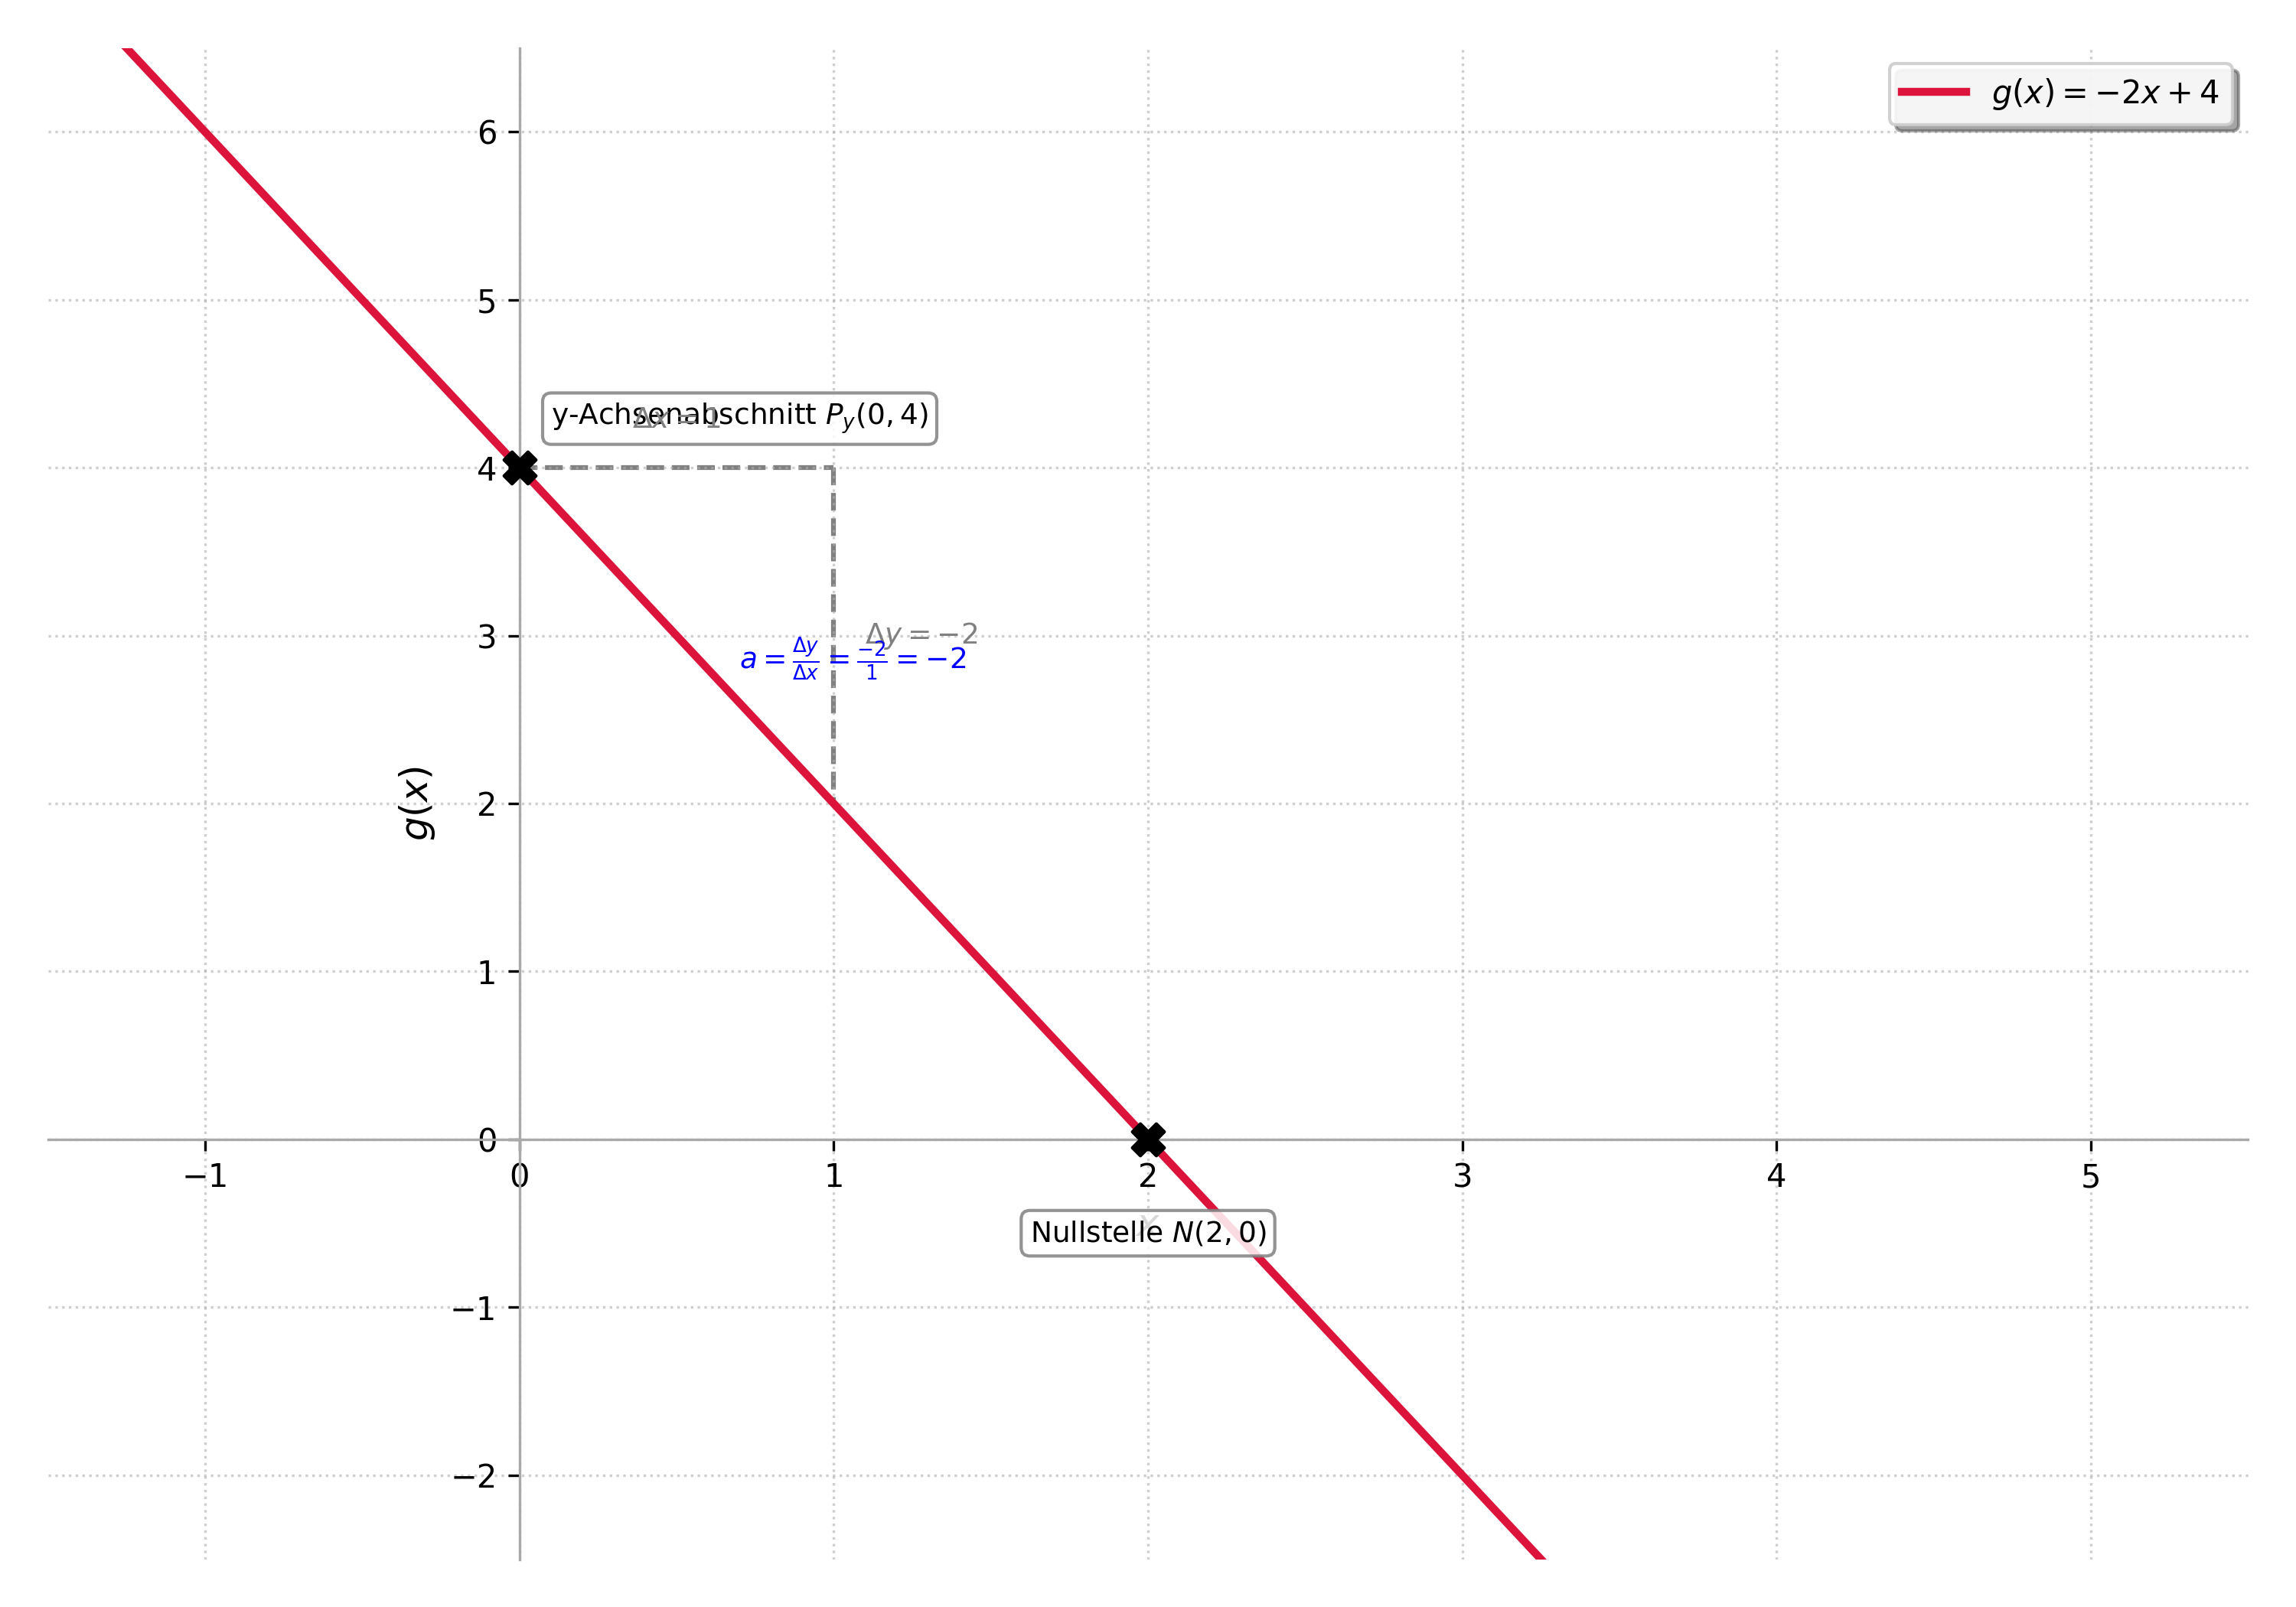
\includegraphics[width=0.8\textwidth]{grafiken/funktion_g_checkliste_graph.png}
    % --- Beschreibung der Grafik für g(x) ---
    % Die Grafik zeigt ein kartesisches Koordinatensystem.
    % Die x-Achse und y-Achse sind beschriftet und sinnvoll skaliert (z.B. von -1 bis 5 für x und -2 bis 6 für y).
    % Eingezeichnet ist der Graph der Funktion g(x) = -2x + 4. Es ist eine Gerade.
    % Die Nullstelle (Schnittpunkt mit der x-Achse) bei (2|0) ist deutlich markiert.
    % Der y-Achsenabschnitt (Schnittpunkt mit der y-Achse) bei (0|4) ist deutlich markiert.
    % Die Gerade fällt, was der negativen Steigung a=-2 entspricht.
    % Ein Steigungsdreieck könnte optional eingezeichnet sein (z.B. 1 Einheit nach rechts, 2 Einheiten nach unten).
    \captionof{figure}{Graph der Funktion $g(x) = -2x + 4$ mit markierten Achsenschnittpunkten.}
    \label{fig:g_checkliste_graph}
    \end{center}
    Der Graph ist eine Gerade, die die y-Achse bei $y=4$ und die x-Achse bei $x=2$ schneidet. Da die Steigung $a=-2$ negativ ist, fällt die Gerade.

    \item \textbf{Vorzeichen der Funktionswerte:}
    Die Nullstelle der Funktion ist $x_0=2$. Die Steigung ist $a=-2$ (negativ).
    \begin{itemize}
        \item \textbf{In welchem Intervall ist $g(x) > 0$?} \\
        Da die Funktion eine negative Steigung hat und bei $x_0=2$ die x-Achse schneidet (also $g(2)=0$), sind die Funktionswerte für alle $x$-Werte links von der Nullstelle positiv (die Gerade kommt von 'oben links').
        Der Graph verläuft oberhalb der x-Achse für $x < 2$. Intervall: $(-\infty, 2)$.
        \item \textbf{In welchem Intervall ist $g(x) < 0$?} \\
        Entsprechend sind die Funktionswerte für alle $x$-Werte rechts von der Nullstelle negativ.
        Der Graph verläuft unterhalb der x-Achse für $x > 2$. Intervall: $(2, \infty)$.
    \end{itemize}

    \item \textbf{Argumentation mit Steigung und Nullstelle:}
    Die Steigung $a=-2$ ist negativ. Das bedeutet, dass die Funktion streng monoton fällt: Wenn $x$ größer wird, wird $g(x)$ kleiner.
    Die Nullstelle ist $x_0=2$, an dieser Stelle ist $g(x_0)=0$.
    Für $x$-Werte, die größer als die Nullstelle sind ($x > x_0$), also rechts von $x_0=2$: Da die Funktion fällt, müssen die Funktionswerte $g(x)$ kleiner sein als der Wert an der Nullstelle ($g(x_0)=0$). Somit muss $g(x) < 0$ (negativ) sein für $x > x_0$.
    (Umgekehrt gilt: Für $x < x_0$ müssen die Funktionswerte größer als $g(x_0)=0$ sein, also $g(x) > 0$ (positiv).)

    \item \textbf{Vergleich mit dem y-Achsenabschnitt:}
    Der y-Achsenabschnitt ist $b=4$, das bedeutet $g(0)=4$.
    Der Funktionswert $g(0)=4$ ist positiv.
    Die Stelle $x=0$ liegt im Intervall $(-\infty, 2)$, für das wir in Teil (c) bestimmt haben, dass $g(x) > 0$ ist.
    Dies bestätigt unsere Überlegungen: Da $x=0 < x_0=2$ ist (also links von der Nullstelle liegt) und die Funktion eine negative Steigung hat (also von links oben nach rechts unten verläuft), muss der Funktionswert bei $x=0$ positiv sein.

    \item \textbf{Gedankenexperiment:}
    Wir stellen uns eine lineare Funktion $h(x)$ vor mit: Steigung $a_h > 0$ (positiv) und Nullstelle $x_{h0} > 0$ (positiv).
    \begin{itemize}
        \item \textbf{Grobe Skizze, wie solch eine Funktion aussehen könnte.}
        \begin{center}
        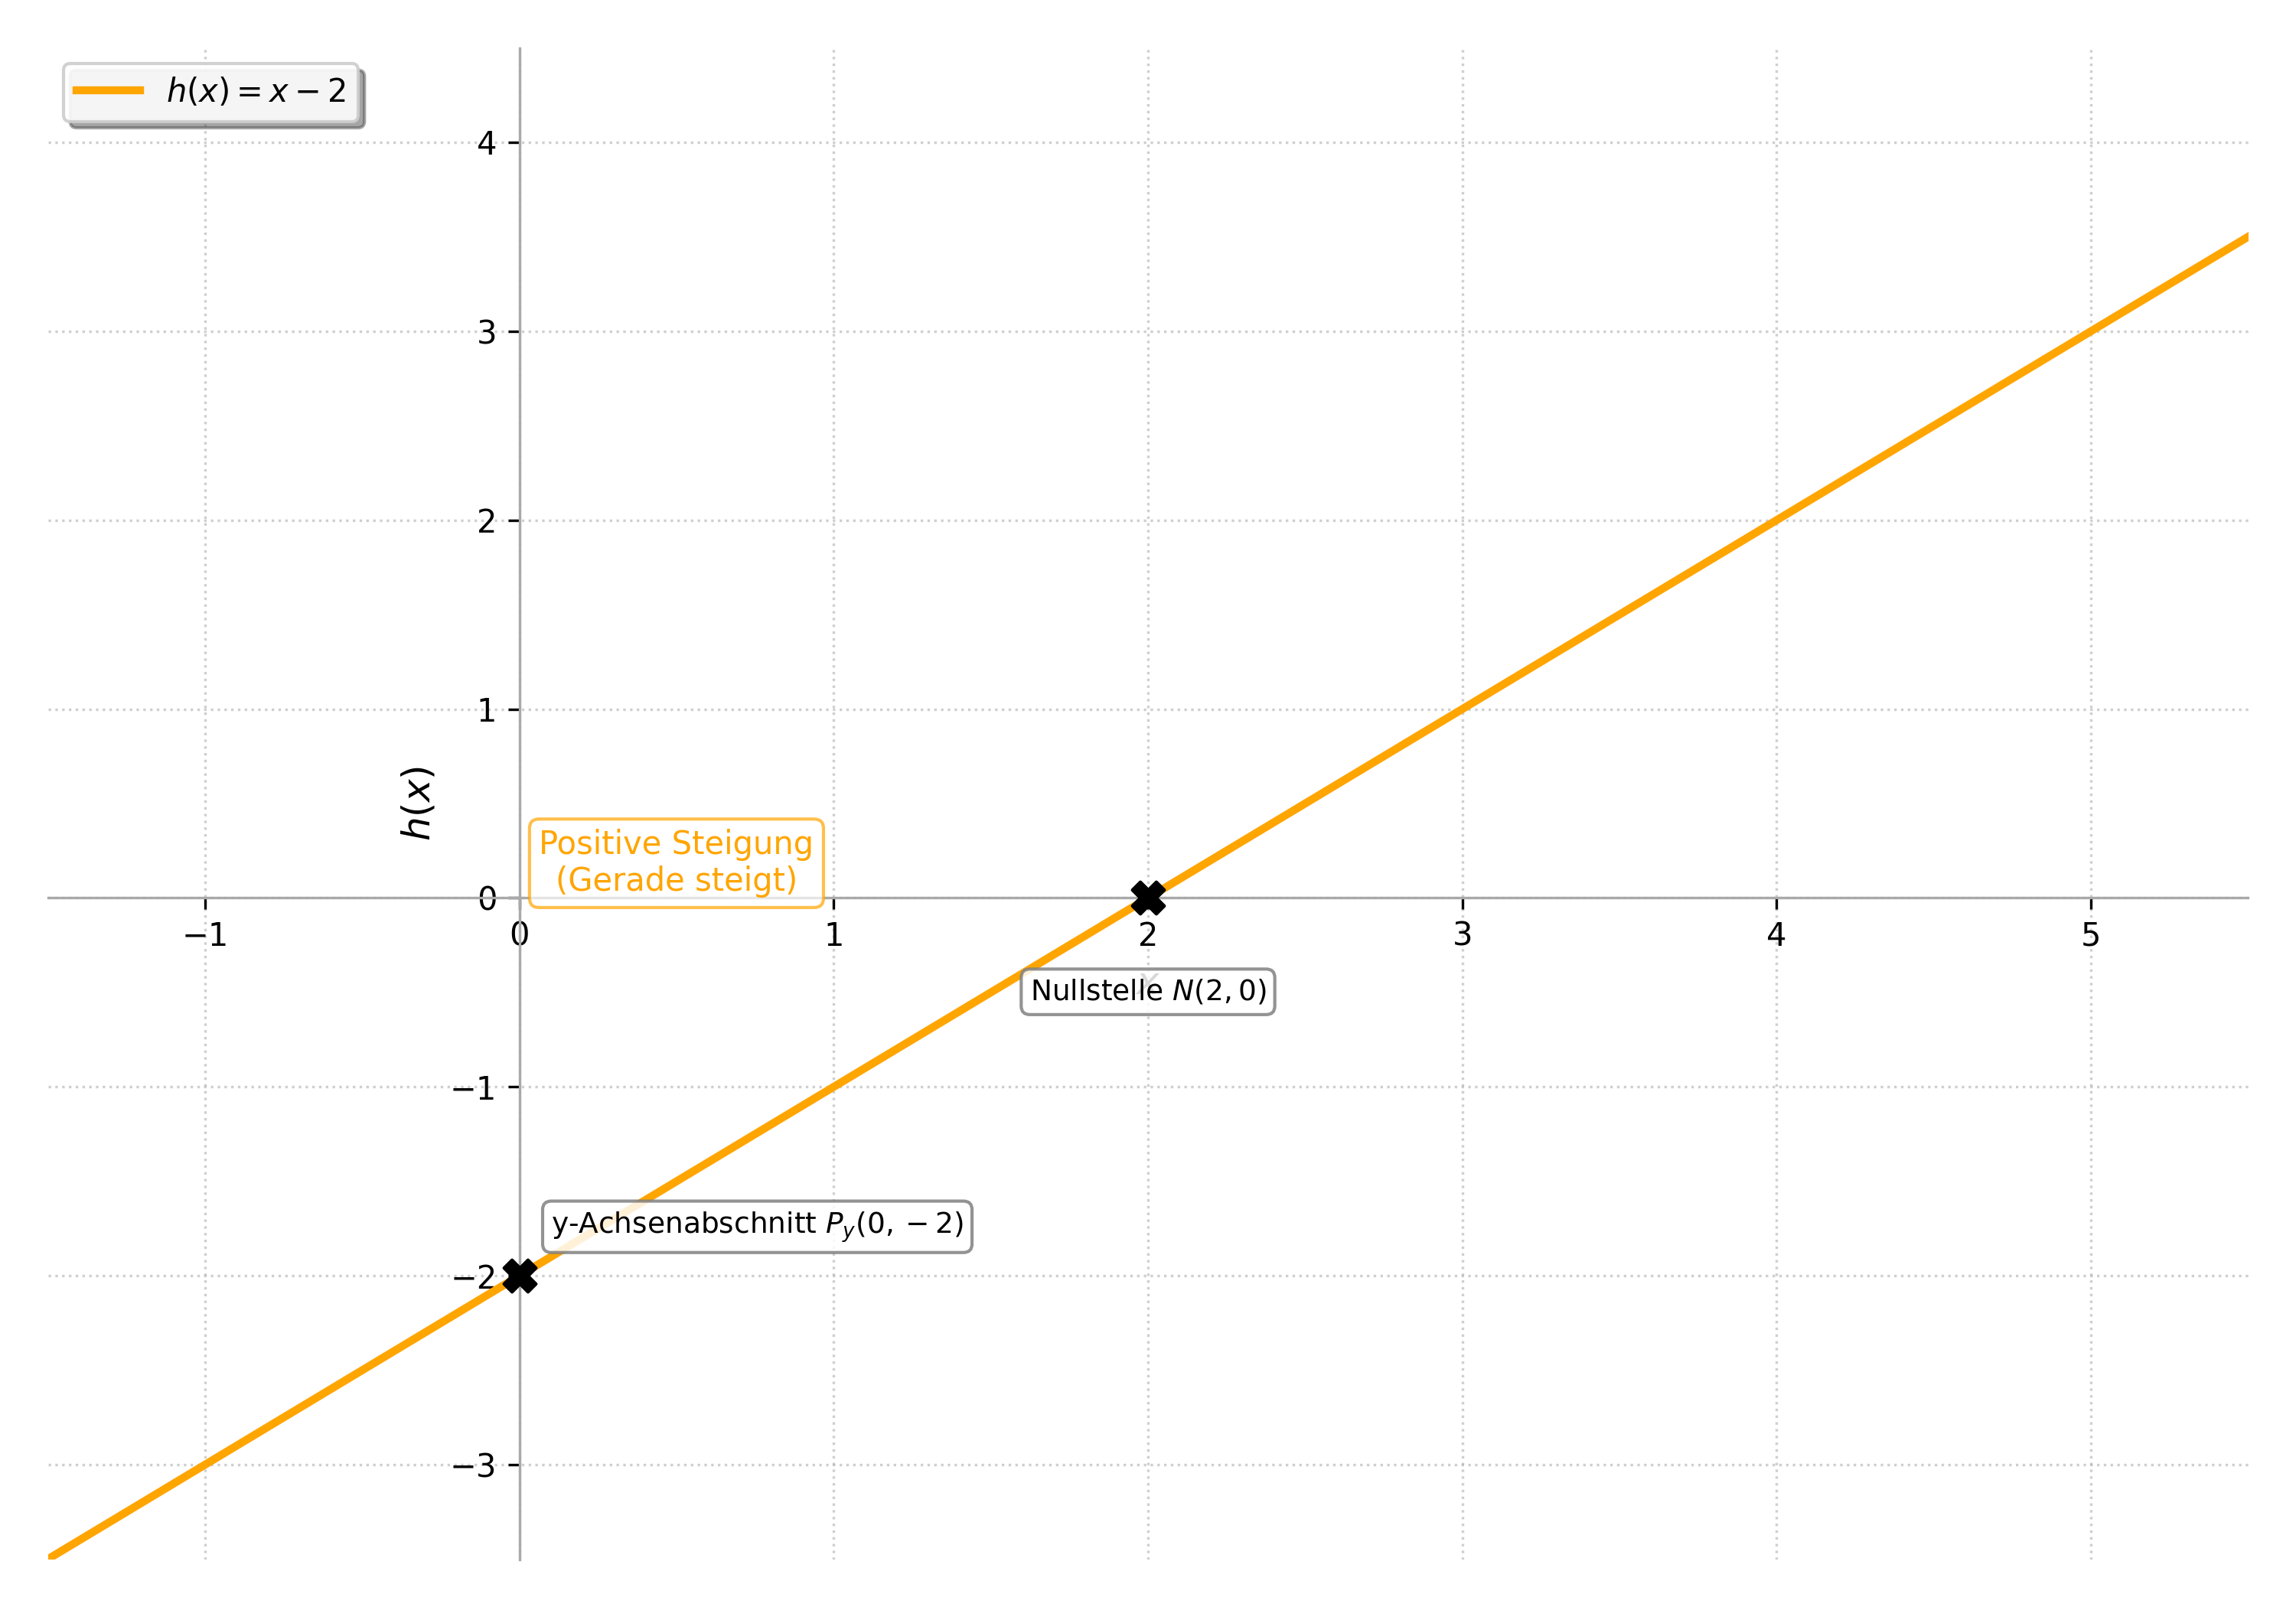
\includegraphics[width=0.8\textwidth]{grafiken/funktion_h_gedankenexperiment_graph.png}
        % --- Beschreibung der Grafik für h(x) ---
        % Die Grafik zeigt ein kartesisches Koordinatensystem.
        % Eine Gerade h(x) ist eingezeichnet, die von links unten nach rechts oben steigt (positive Steigung).
        % Diese Gerade schneidet die x-Achse im positiven Bereich (rechts vom Ursprung, da x_h0 > 0).
        % Folglich muss die Gerade die y-Achse unterhalb des Ursprungs schneiden.
        \captionof{figure}{Skizze einer linearen Funktion $h(x)$ mit positiver Steigung und positiver Nullstelle.}
        \label{fig:h_gedankenexperiment_graph}
        \end{center}

        \item \textbf{Welches Vorzeichen muss der y-Achsenabschnitt dieser Funktion $h(x)$ haben? Begründe.} \\
        Der y-Achsenabschnitt $b_h$ dieser Funktion $h(x)$ muss \textbf{negativ} sein.

        \textbf{Begründung anhand der Skizze:}
        Wenn eine Gerade eine positive Steigung hat (also von links unten nach rechts oben verläuft) und ihre Nullstelle im positiven $x$-Bereich liegt (d.h., sie schneidet die x-Achse rechts vom Ursprung), dann muss sie die y-Achse ($x=0$) unterhalb der x-Achse geschnitten haben, um diesen positiven $x$-Achsenabschnitt zu erreichen. Ein Schnittpunkt mit der y-Achse unterhalb der x-Achse bedeutet einen negativen y-Achsenabschnitt.

        \textbf{Mathematische Begründung:}
        Die allgemeine Form der linearen Funktion ist $h(x) = a_h x + b_h$.
        An der Nullstelle $x_{h0}$ gilt $h(x_{h0}) = 0$:
        $$ a_h x_{h0} + b_h = 0 $$
        Wir lösen nach dem y-Achsenabschnitt $b_h$ auf:
        $$ b_h = -a_h x_{h0} $$
        Wir wissen:
        \begin{itemize}
            \item Die Steigung $a_h$ ist positiv ($a_h > 0$).
            \item Die Nullstelle $x_{h0}$ ist positiv ($x_{h0} > 0$).
        \end{itemize}
        Das Produkt zweier positiver Zahlen $a_h \cdot x_{h0}$ ist ebenfalls positiv.
        Da $b_h = -(a_h x_{h0})$ ist, und $a_h x_{h0}$ positiv ist, muss $b_h$ negativ sein (z.B. wenn $a_h x_{h0} = 5$, dann ist $b_h = -5$).
    \end{itemize}
\end{enumerate}

\end{loesungsumgebung} %überarbeitet mit weißt du noch etc
\section{Quadratische Funktionen – Die Welt der Parabeln}
\label{sec:quadratische-funktionen}

Nach den Geraden, die von linearen Funktionen beschrieben werden, wenden wir uns nun einer weiteren wichtigen Funktionsklasse zu: den \textbf{quadratischen Funktionen}. Ihre Graphen sind keine Geraden mehr, sondern elegante Kurven, die \textbf{Parabeln} genannt werden. Du wirst sehen, dass diese Parabeln in vielen Bereichen der Natur und Technik eine Rolle spielen und dass wir mit den richtigen Werkzeugen auch ihre Eigenschaften genau untersuchen können.

\begin{tcolorbox}[colback=blue!5!white, colframe=blue!75!black, title=Was du in diesem Kapitel lernen wirst:]
Nachdem du dieses Kapitel durchgearbeitet hast, wirst du in der Lage sein:
\begin{itemize}[noitemsep, topsep=0pt, leftmargin=*, itemsep=2pt] % itemsep für leichten Abstand
    \item zu erklären, was eine quadratische Funktion ist, ihren Graphen (die Parabel) zu erkennen und Beispiele aus Alltag und Technik zu nennen.
    \item die \textbf{Normalform} $f(x) = ax^2+bx+c$ zu nutzen und die Bedeutung der Parameter $a, b, c$ für Öffnungsrichtung, Form (Stauchung/Streckung) und den y-Achsenabschnitt der Parabel zu interpretieren.
    \item den \textbf{Scheitelpunkt} $S(x_S|y_S)$ einer Parabel mit der Formel $x_S = -b/(2a)$ zu berechnen und die Funktion durch \textbf{quadratische Ergänzung} in die \textbf{Scheitelpunktform} $f(x)=a(x-x_S)^2+y_S$ umzuwandeln, um den Scheitelpunkt direkt abzulesen.
    \item die \textbf{Nullstellen} quadratischer Funktionen mit der Mitternachtsformel oder der p-q-Formel zu bestimmen, die Rolle der Diskriminante zu verstehen und die \textbf{faktorisierte Form} $f(x)=a(x-x_1)(x-x_2)$ zu nutzen.
    \item die \textbf{Symmetrieeigenschaften} von Parabeln (insbesondere die Achsensymmetrie zur Geraden $x=x_S$) zu verstehen und anzuwenden.
    \item eine vollständige \textbf{Kurvendiskussion} für quadratische Funktionen durchzuführen, d.h. alle wesentlichen Eigenschaften zu analysieren und den Graphen sorgfältig zu zeichnen.
    \item \textbf{Anwendungsaufgaben} (z.B. Flugbahnen, Optimierungsprobleme) mit quadratischen Funktionen zu modellieren und zu lösen.
    \item die notwendigen \textbf{algebraischen Werkzeuge} (binomische Formeln, Termumformungen, Umgang mit Potenzen und Brüchen) sicher einzusetzen.
    \item ein tiefgehendes qualitatives Verständnis für die Zusammenhänge zwischen den verschiedenen Darstellungsformen, Parametern, besonderen Punkten und dem Graphen einer Parabel zu entwickeln.
    \item einen ersten Einblick in Funktionen mit höheren Potenzen
\end{itemize}
\end{tcolorbox}
\bigskip

\begin{infoboxumgebung}{Was bedeutet 'quadratisch' und wo begegnet es uns?}
Das Wort 'quadratisch' erinnert dich vielleicht an das 'Quadrat' einer Zahl, also eine Zahl mit sich selbst multipliziert (z.B. $3^2 = 3 \cdot 3 = 9$). Genau das ist der Kern: In einer quadratischen Funktion kommt die Variable (meistens $x$) in der zweiten Potenz vor, also als $x^2$.

Parabeln findest du überall:
\begin{itemize}
    \item Die \textbf{Flugbahn} eines Balls, den du wirfst, oder eines Wasserstrahls aus einem Springbrunnen ist (unter idealisierten Bedingungen ohne Luftwiderstand) eine Parabel.
    \item \textbf{Satellitenschüsseln} und die Reflektoren in \textbf{Autoscheinwerfern} sind oft parabelförmig (genauer: Paraboloid, eine 3D-Parabel). Diese Form hat die tolle Eigenschaft, parallel einfallende Strahlen (Funkwellen oder Licht) in einem Punkt, dem Brennpunkt, zu sammeln – oder umgekehrt, Licht von einer Quelle im Brennpunkt parallel auszusenden.
    \item Die \textbf{Kabel von Hängebrücken} bilden unter der Last der Fahrbahn annähernd eine Parabelform.
    \item In der Physik beschreiben quadratische Funktionen oft Zusammenhänge mit \textbf{gleichmäßiger Beschleunigung}, z.B. den zurückgelegten Weg beim freien Fall.
    \item Viele \textbf{Optimierungsprobleme} führen auf quadratische Funktionen: Wann ist eine Fläche bei gegebenem Umfang maximal? Bei welcher Produktionsmenge sind die Kosten minimal?
\end{itemize}
Du siehst, es lohnt sich, diese Funktionsart genauer kennenzulernen!
\end{infoboxumgebung}

\subsection{Die allgemeine Form und erste Eigenschaften}

Jede quadratische Funktion lässt sich in einer Standardform schreiben, die uns erste Hinweise auf das Aussehen ihres Graphen gibt.

\begin{merksatzumgebung}[Allgemeine Form und Parameter]{Die quadratische Funktion in Normalform}\label{merksatz_quadratische_normalform}
Die \textbf{allgemeine Form} (auch \textbf{Normalform} oder Polynomform zweiten Grades genannt) einer quadratischen Funktion lautet:
\[ f(x) = ax^2 + bx + c \]
Dabei sind $a, b, c$ reelle Zahlen, die man \textbf{Koeffizienten} oder \textbf{Parameter} der Funktion nennt.
\begin{itemize}
    \item Der Koeffizient $a$ (vor dem $x^2$) ist der \textbf{Öffnungsfaktor} oder \textbf{Streckfaktor}.
        \begin{itemize}
            \item Er darf \textbf{nicht Null} sein ($a \neq 0$), sonst wäre der $x^2$-Term nicht vorhanden und die Funktion wäre linear ($f(x)=bx+c$) oder konstant ($f(x)=c$, falls auch $b=0$).
            \item Das \textbf{Vorzeichen von $a$} bestimmt die \textbf{Öffnungsrichtung} der Parabel:
                \begin{itemize}
                    \item $a > 0$: Die Parabel ist \textbf{nach oben geöffnet} (wie ein Tal oder ein lachender Mund $\smile$). Intuitiv: Für sehr große positive oder negative $x$-Werte wird $x^2$ sehr groß und positiv. Multipliziert mit einem positiven $a$ bleibt das Ergebnis groß und positiv, die $y$-Werte gehen also nach oben.
                    \item $a < 0$: Die Parabel ist \textbf{nach unten geöffnet} (wie ein Berg oder ein trauriger Mund $\frown$). Intuitiv: Für sehr große $x$-Werte wird $x^2$ sehr groß und positiv. Multipliziert mit einem negativen $a$ wird das Ergebnis groß und negativ, die $y$-Werte gehen also nach unten.
                \end{itemize}
            \item Um die Form der Parabel (ihre Breite oder Schmalheit) zu beschreiben, verwenden wir den \textbf{Betrag} von $a$.
                
                \textit{Kurze Erinnerung zum Betrag einer Zahl:} Der Betrag einer Zahl $x$, geschrieben als $|x|$, ist ihr Abstand von der Null auf dem Zahlenstrahl. Der Betrag ist immer eine nicht-negative Zahl (also positiv oder Null).
                \begin{itemize}[nosep, leftmargin=2em] % enumitem Option für kompakte Liste
                    \item Ist eine Zahl $x$ \textbf{positiv oder Null}, ist ihr Betrag sie selbst: $|x|=x$. \\ Beispiele: $|7| = 7$; $|0| = 0$.
                    \item Ist eine Zahl $x$ \textbf{negativ}, ist ihr Betrag die positive Gegenzahl: $|x|=-x$. \\ Beispiel: $|-3| = -(-3) = 3$.
                \end{itemize}
                Der Betrag $|a|$ gibt uns also den Wert von $a$ ohne sein Vorzeichen an.

            \item Der nun erklärte \textbf{Betrag von $a$} (also $|a|$) bestimmt die \textbf{Form (Breite/Schmalheit)} der Parabel im Vergleich zur \textit{Normalparabel} $y=x^2$ (bei der $a=1$ ist):
                \begin{itemize}
                    \item $|a| > 1$: Die Parabel ist \textbf{gestreckter} (schmaler, steiler) als die Normalparabel.
                    \item $0 < |a| < 1$: Die Parabel ist \textbf{gestauchter} (breiter, flacher) als die Normalparabel.
                    \item $|a| = 1$: Die Parabel hat dieselbe Öffnungsweite wie die Normalparabel.
                \end{itemize}
        \end{itemize}
    \item Der Koeffizient $b$ (vor dem $x$) beeinflusst zusammen mit $a$ die \textbf{Lage des Scheitelpunkts} und damit die Position der Parabel im Koordinatensystem (Verschiebung nach links/rechts und oben/unten). Ist $b=0$, liegt der Scheitelpunkt auf der y-Achse.
    \item Der Koeffizient $c$ ist der \textbf{y-Achsenabschnitt}. Er gibt direkt den y-Wert an, bei dem die Parabel die y-Achse schneidet. Denn für $x=0$ ist $f(0) = a \cdot 0^2 + b \cdot 0 + c = c$. Der Schnittpunkt mit der y-Achse ist also immer $P_y(0|c)$.
\end{itemize}
\end{merksatzumgebung}

Allein aus diesen drei Koeffizienten $a, b, c$ können wir also schon eine Menge über die Parabel aussagen!

\begin{aufgabenumgebung}{Parameter-Check}
Betrachte die folgenden quadratischen Funktionen. Gib für jede Funktion die Werte der Koeffizienten $a, b$ und $c$ an. Was kannst du sofort über die Öffnungsrichtung, die Form (schmaler/breiter als Normalparabel) und den y-Achsenabschnitt sagen?
\begin{enumerate}
    \item $f(x) = 2x^2 - 4x + 5$
    \item $g(x) = -x^2 + 3x - 1$
    \item $h(x) = 0.25x^2 + 2$ (Achtung, welcher Koeffizient ist hier Null?)
    \item $k(x) = -3x^2 - 6x$ (Und hier?)
\end{enumerate}
\end{aufgabenumgebung}

\begin{funfactbox}{Quadratzahlen zum Anfassen – Ein Trick mit ungeraden Zahlen!}
Du weißt, dass $3^2 = 9$ oder $4^2 = 16$ bedeutet. Aber wusstest du, dass du jede Quadratzahl auch durch das Addieren einer Reihe von aufeinanderfolgenden ungeraden Zahlen erhalten kannst? Schau mal:
\begin{itemize}
    \item $1 = \mathbf{1}^2$
    \item $1 + 3 = 4 = \mathbf{2}^2$
    \item $1 + 3 + 5 = 9 = \mathbf{3}^2$
    \item $1 + 3 + 5 + 7 = 16 = \mathbf{4}^2$
    \item $1 + 3 + 5 + 7 + 9 = 25 = \mathbf{5}^2$
\end{itemize}
Erkennst du das Muster? Die Summe der ersten $n$ ungeraden Zahlen ergibt immer $n^2$!
So verbirgt sich hinter einfachen Additionen eine direkte Verbindung zu den quadratischen Zahlen, die den quadratischen Funktionen ihren Namen geben. Dieses Muster lässt sich sogar geometrisch darstellen, indem man Quadrate aus 'L-förmigen' Anbauten aus einer ungeraden Anzahl von Kästchen zusammensetzt. Eine schöne Verbindung zwischen Arithmetik und Geometrie!

\begin{center}
    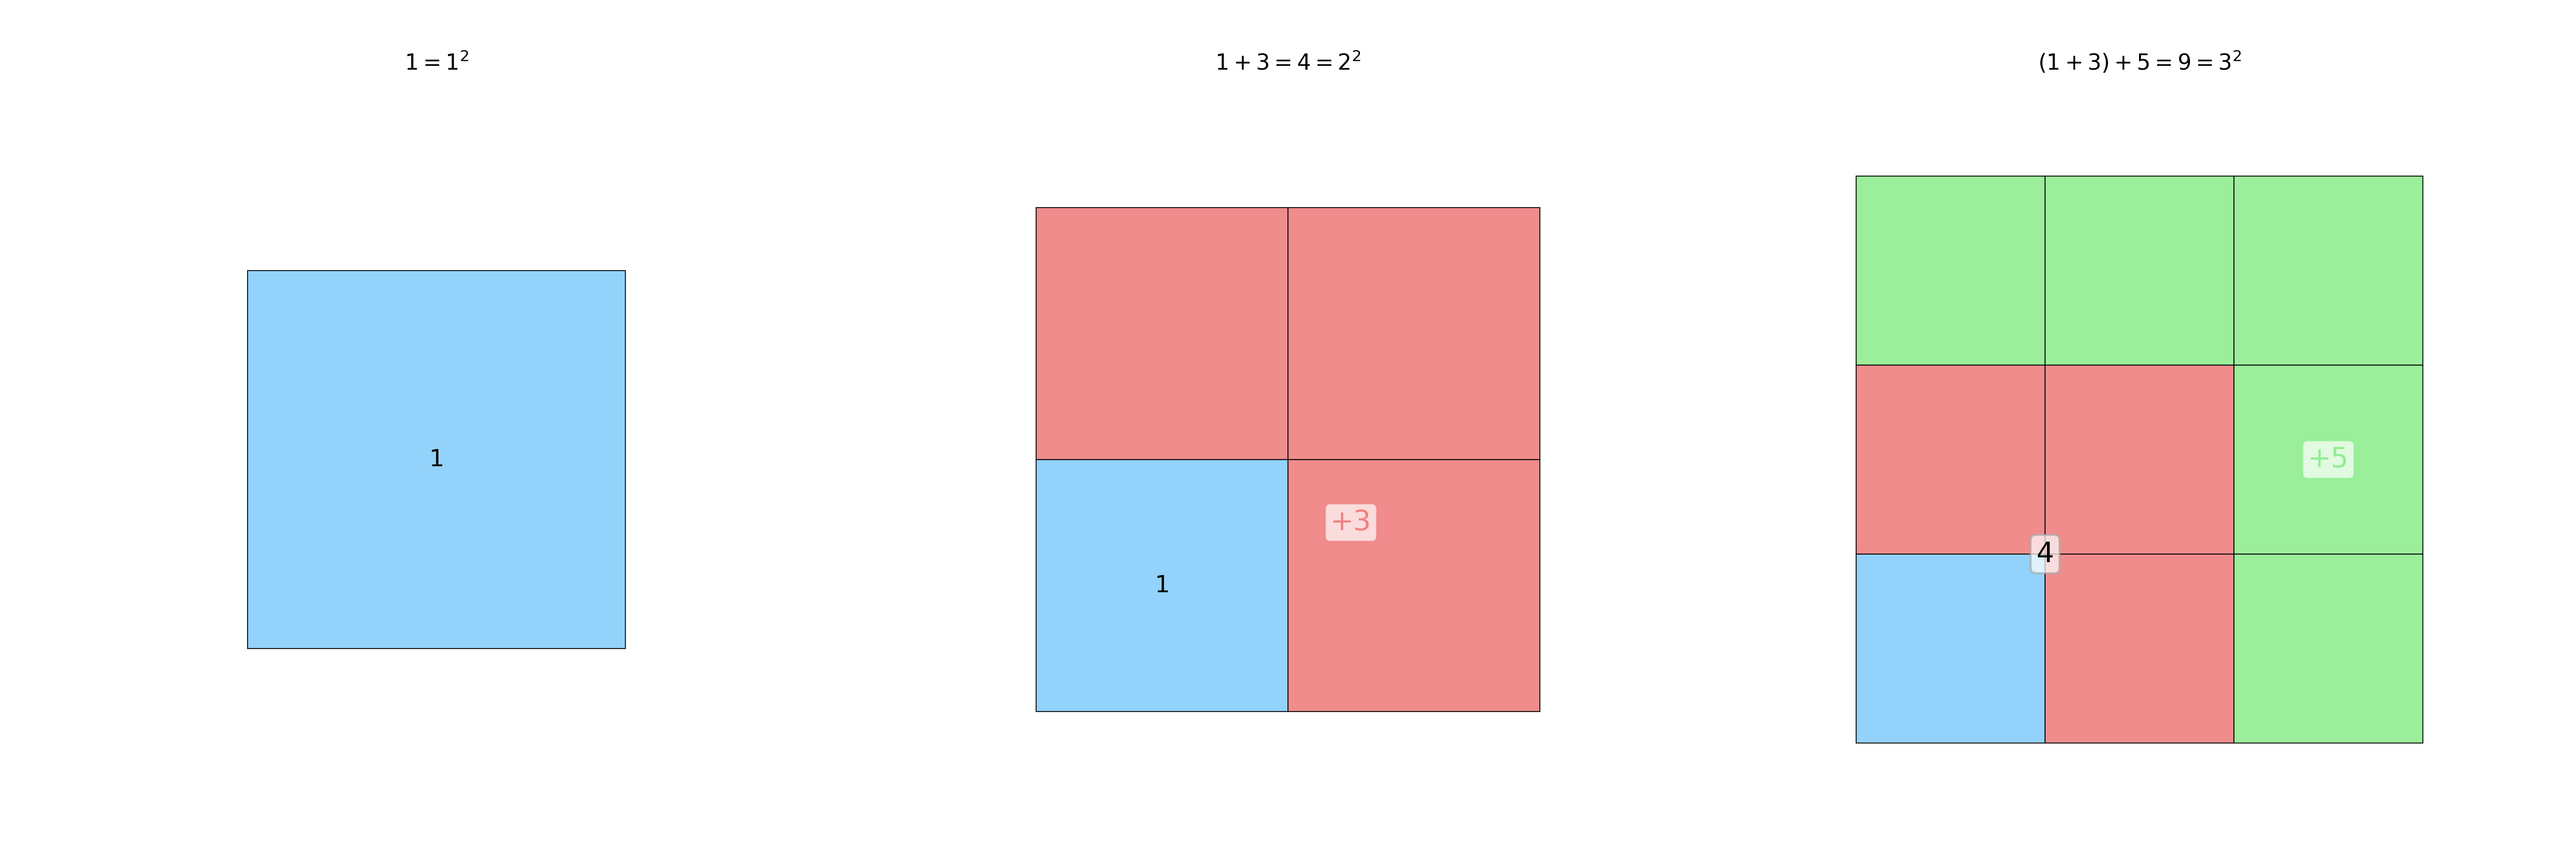
\includegraphics[width=0.5\textwidth]{grafiken/Summe_Ungerade_Zahlen_Quadrate.png}
    % Beschreibung für die Grafik 'Summe_Ungerade_Zahlen_Quadrate.png':
    % Die Grafik könnte zeigen, wie Quadratzahlen durch das Hinzufügen 
    % L-förmiger 'Schalen' aus einer ungeraden Anzahl von Blöcken wachsen:
    % - Ein einzelner Block (1 = 1^2).
    % - Ein 1x1 Block, an den 3 Blöcke L-förmig angefügt werden, um einen 2x2 Block zu bilden (1+3 = 2^2).
    % - Ein 2x2 Block, an den 5 Blöcke L-förmig angefügt werden, um einen 3x3 Block zu bilden (4+5 = 3^2).
    % Die jeweils hinzugefügten Blöcke sollten farblich hervorgehoben sein.
    \captionof{figure}{Geometrische Darstellung: Summe ungerader Zahlen ergibt Quadratzahlen.}
    \label{fig:summe_ungerade_quadrate}
\end{center}
\end{funfactbox}
\subsection{Grafische Darstellung – So sehen Parabeln aus}

Die grafische Darstellung einer quadratischen Funktion ist immer eine Parabel. Ihre genaue Form und Lage hängt von den Parametern $a, b, c$ ab.

\begin{infoboxumgebung}{Digitale Helfer: Funktionsplotter und Analyse-Tools}
Wenn du den Graphen einer Funktion schnell visualisieren möchtest oder die Berechnung von besonderen Punkten (Nullstellen, Extrempunkte, Wendepunkte) sehr aufwendig wird, gibt es nützliche digitale Werkzeuge, die dir helfen können. Seiten wie \textbf{Wolfram Alpha} (wolframalpha.com) oder grafikfähige Taschenrechner bzw. Mathematik-Software (z.B. GeoGebra) sind hier sehr mächtig.

\textbf{Was können diese Werkzeuge für dich tun?}
\begin{itemize}
    \item \textbf{a) Graphen zeichnen lassen:} Du kannst einfach eine Funktionsgleichung als Text eingeben (z.B. \verb|plot x^3 - 3x^2 + 4|) und erhältst sofort eine genaue Zeichnung des Graphen. Das ist super, um deine eigenen Skizzen zu überprüfen oder ein Gefühl für den Verlauf komplexerer Funktionen zu bekommen.
    \item \textbf{b) Wichtige Punkte bestimmen lassen:} Diese Tools können oft auch automatisch besondere Punkte berechnen und anzeigen, wie:
    \begin{itemize}
        \item Nullstellen (Schnittpunkte mit der x-Achse)
        \item Extrempunkte (Hoch- und Tiefpunkte)
        \item Wendepunkte
    \end{itemize}
\end{itemize}

\textbf{Was bedeutet 'numerisch finden'?}
Manchmal lassen sich Gleichungen (z.B. zur Bestimmung von Nullstellen oder Extrempunkten) nicht exakt mit den Formeln lösen, die du kennst, besonders bei Polynomen höheren Grades oder komplizierten Funktionen. Dann verwenden diese Computerprogramme oft \textbf{numerische Verfahren}.
Stell dir 'numerisch' so vor: Das Programm probiert nicht eine exakte Formel aus, sondern nähert sich der Lösung schrittweise immer genauer an, bis das Ergebnis eine bestimmte Genauigkeit erreicht hat. Es rechnet also mit Zahlenwerten ('numerus' ist Latein für Zahl), um eine gute Näherung für die gesuchten Punkte zu finden. Das Ergebnis ist dann meist ein Dezimalwert, z.B. $x \approx 1.769$.

\textbf{Ein kleines Beispiel für Wolfram Alpha:}
Wenn du die Funktion $f(x) = x^3 - 2x^2 - 5x + 6$ untersuchen möchtest, von der wir vielleicht schon wissen, dass eine Nullstelle $x_1=1$ ist, aber die anderen nicht so leicht zu finden sind:
\begin{itemize}
    \item \textbf{Mögliche Eingaben könnten sein:}
        \begin{itemize}
            \item Um den Graphen zu sehen: \verb|plot x^3 - 2x^2 - 5x + 6|
            \item Um direkt nach Nullstellen zu fragen: \verb|roots of x^3 - 2x^2 - 5x + 6|
            \item Um nach lokalen Extrema zu fragen: \verb|local extrema of x^3 - 2x^2 - 5x + 6|
        \end{itemize}
    \item \textbf{Mögliche Ergebnisse (Wolfram Alpha zeigt vieles davon an):}
    \begin{itemize}
        \item Ein Graph der Funktion.
        \item \textbf{Roots (Nullstellen):} z.B. $x=-2$, $x=1$, $x=3$.
        \item \textbf{Local maximum/minimum (Extrempunkte):} z.B. lokales Maximum bei $x \approx -0.786$, lokales Minimum bei $x \approx 2.12$.
        \item \textbf{Inflection point (Wendepunkt):} z.B. bei $x \approx 0.667$.
    \end{itemize}
\end{itemize}
Diese Werkzeuge sind also eine tolle Ergänzung, um deine eigenen Rechnungen zu überprüfen und ein tieferes visuelles Verständnis zu entwickeln. Sie ersetzen aber nicht das grundlegende Verständnis der Konzepte und Rechenwege, die du in diesem Buch lernst – denn nur so weißt du, was du das Werkzeug fragen musst und ob seine Antwort sinnvoll ist!
\end{infoboxumgebung}

\begin{beispielumgebung}[Typische Parabeln]{Beispiele für Parabeln und ihre Graphen}
Schauen wir uns ein paar typische Beispiele an, um ein Gefühl dafür zu bekommen, wie die Parameter den Graphen beeinflussen:

\begin{enumerate}
    \item \textbf{Die Normalparabel:} $f(x) = x^2$
        Hier ist $a=1, b=0, c=0$. Sie ist nach oben geöffnet, hat die 'normale' Breite und ihr Scheitelpunkt (tiefster Punkt) liegt im Ursprung $(0|0)$.
    \item \textbf{Gestauchte, nach oben geöffnete Parabel, verschoben:} $g(x) = 0.5x^2 - 2$
        Hier ist $a=0.5$ (nach oben geöffnet, breiter), $b=0$, $c=-2$. Der y-Achsenabschnitt ist bei $-2$. Da $b=0$, liegt der Scheitelpunkt auf der y-Achse, nämlich bei $S(0|-2)$.
    \item \textbf{Nach unten geöffnete Parabel, verschoben:} $h(x) = -x^2 + 4x - 3$
        Hier ist $a=-1$ (nach unten geöffnet, normale Breite), $b=4$, $c=-3$. Der y-Achsenabschnitt ist bei $-3$. Der Scheitelpunkt liegt nicht auf der y-Achse, da $b \neq 0$. Wir werden später lernen, ihn exakt zu berechnen. Für $h(x)$ liegt er bei $S(2|1)$.
\end{enumerate}
\end{beispielumgebung}

\begin{center}
    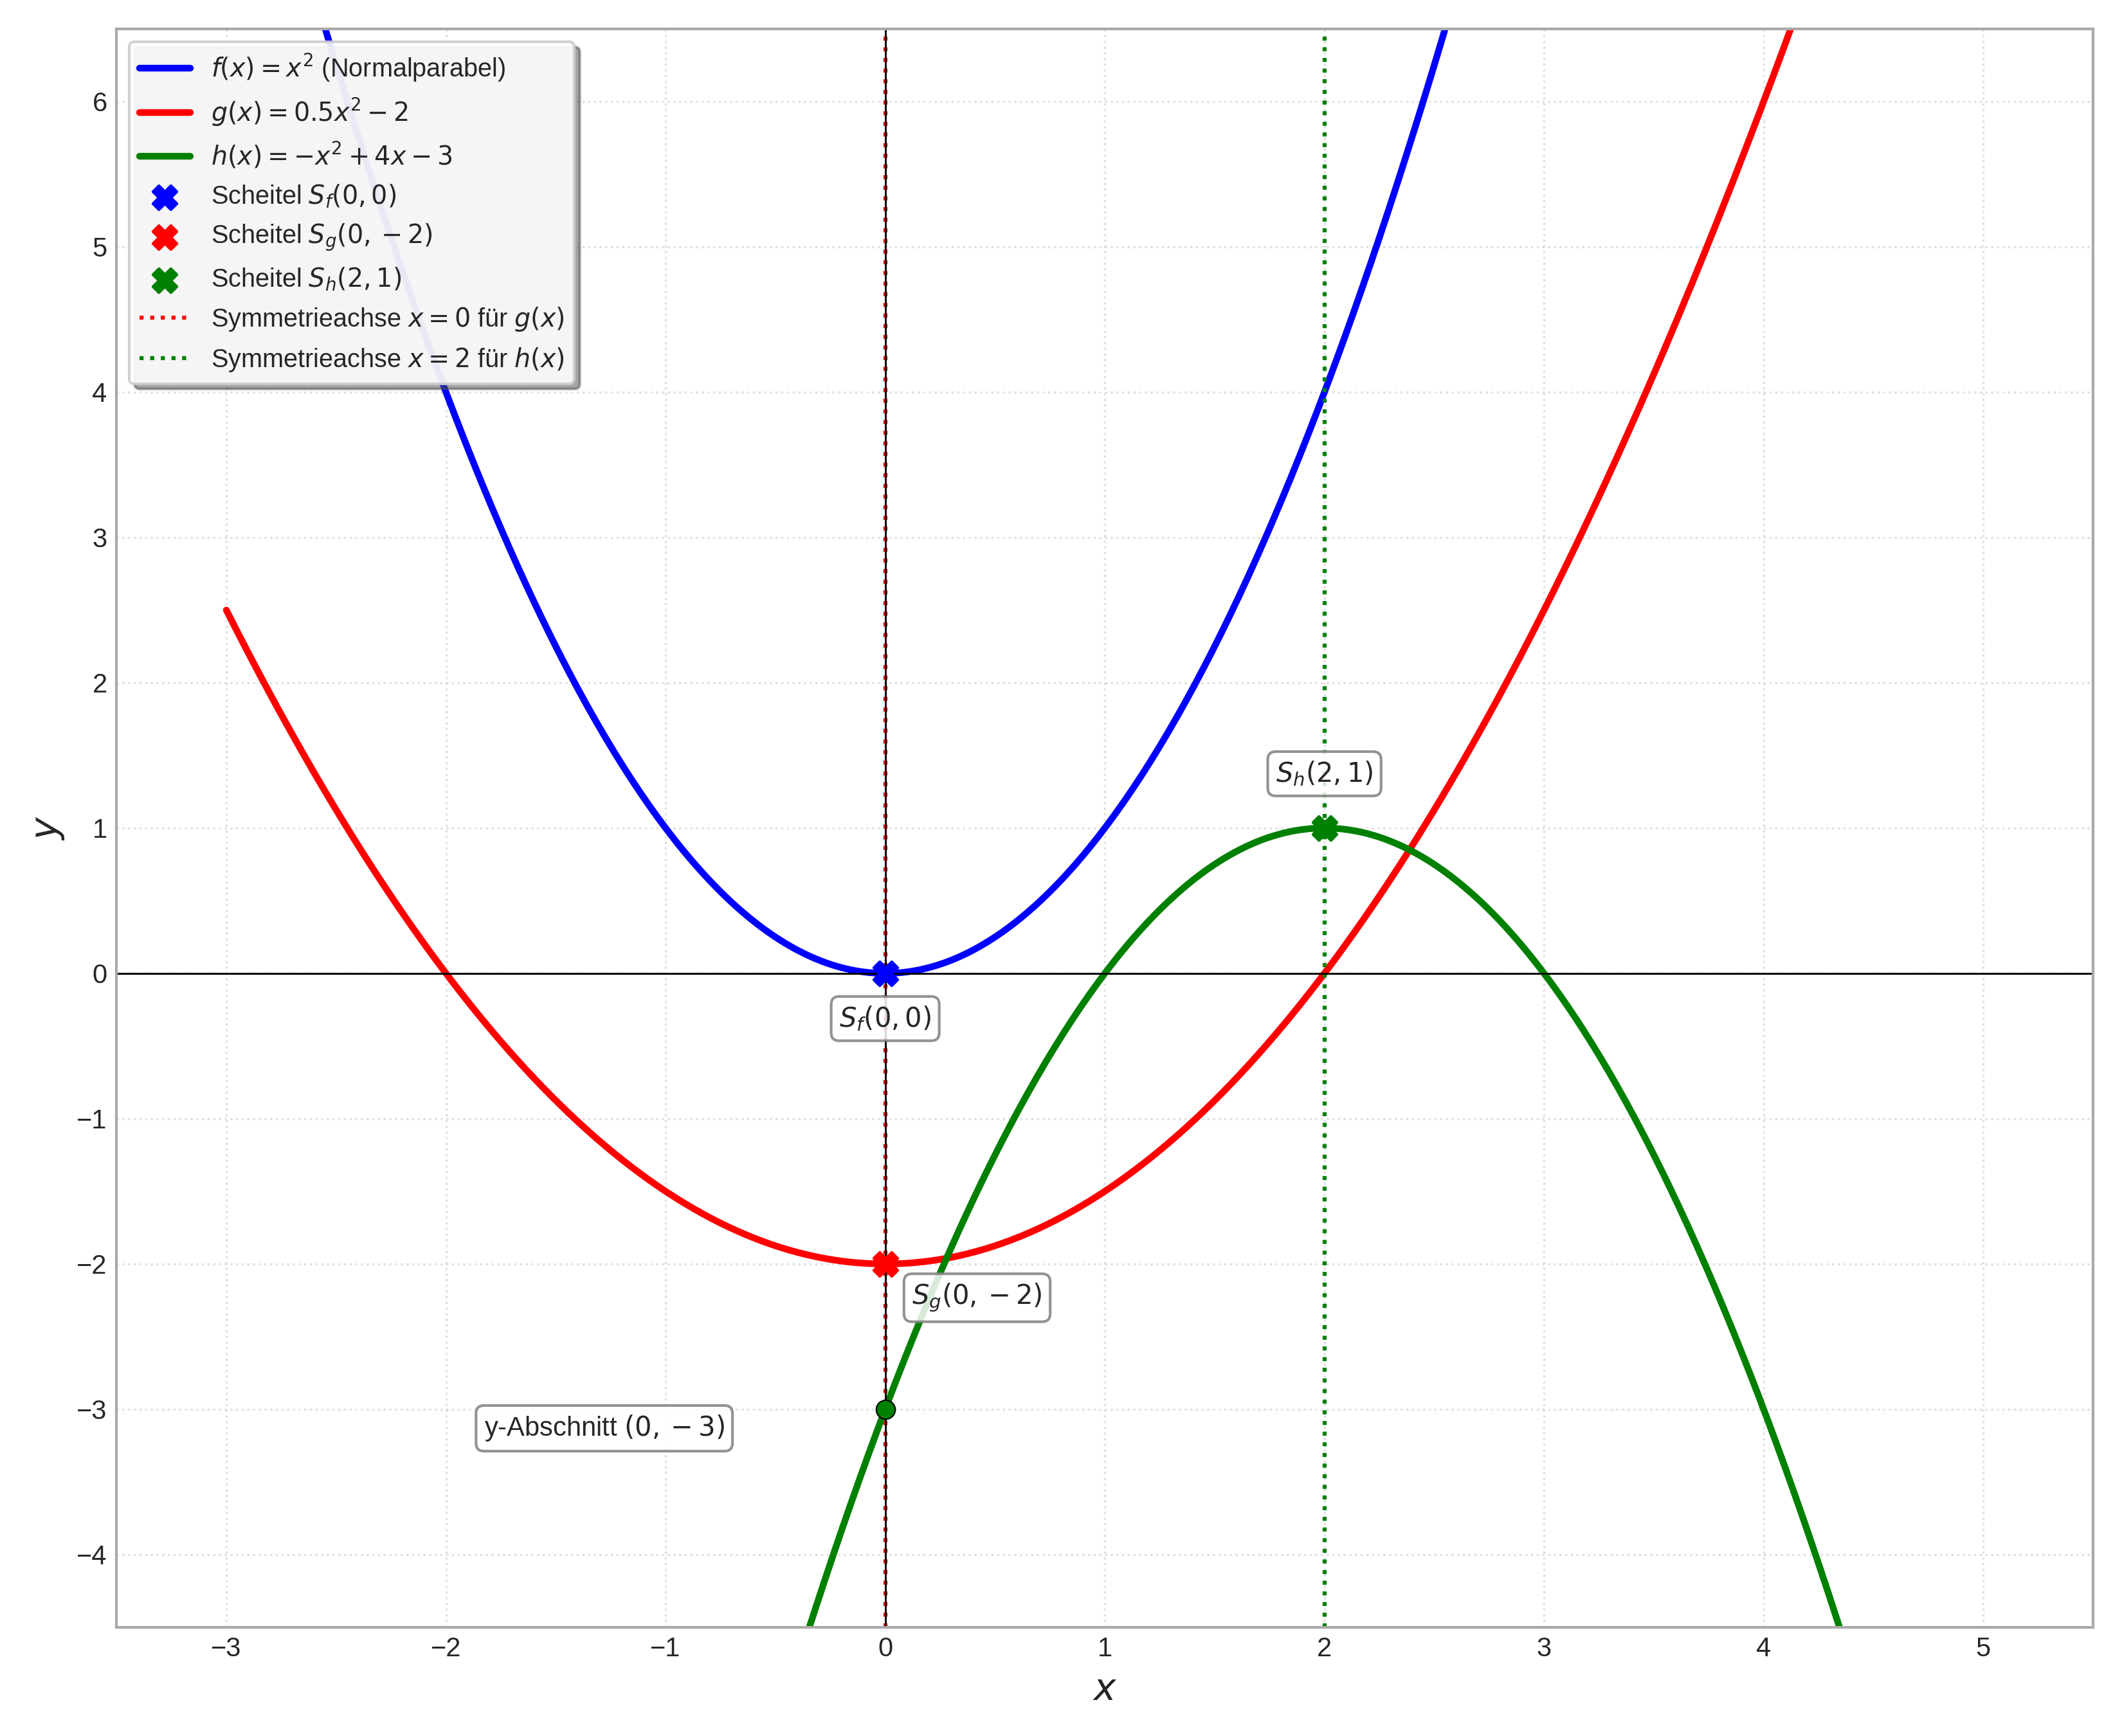
\includegraphics[width=0.9\textwidth]{grafiken/Quadratische_Funktionen_Beispiele.png}
    \captionof{figure}{Verschiedene Parabeln und ihre Eigenschaften}
    \label{fig:parabel_beispiele}
\end{center}
% Der Text geht hier direkt weiter


Um eine Parabel ungefähr zu skizzieren, kannst du eine Wertetabelle anlegen, wie du es von linearen Funktionen kennst. Wähle einige x-Werte, berechne die zugehörigen y-Werte $f(x)$ und trage die Punkte $(x|f(x))$ in ein Koordinatensystem ein. Verbinde die Punkte dann zu einer glatten Kurve.

\begin{aufgabenumgebung}{Parabeln skizzieren mit Wertetabelle}
\begin{enumerate}
    \item Erstelle eine Wertetabelle für die Normalparabel $f(x)=x^2$ für $x$-Werte von $-3$ bis $3$ (in Einerschritten). Zeichne den Graphen.
    \item Erstelle eine Wertetabelle für $g(x)=2x^2$ für dieselben x-Werte. Zeichne den Graphen in dasselbe Koordinatensystem wie $f(x)$. Was beobachtest du im Vergleich zur Normalparabel?
    \item Erstelle eine Wertetabelle für $h(x)=-0.5x^2+1$ für dieselben x-Werte. Zeichne den Graphen ebenfalls in dasselbe Koordinatensystem. Was beobachtest du?
\end{enumerate}
\end{aufgabenumgebung}



\begin{erinnerungsboxumgebung}{Algebra-Fitness für quadratische Funktionen}
Bei quadratischen Funktionen werden wir oft Terme umformen, Klammern auflösen und mit Potenzen rechnen. Ein sicherer Umgang mit den folgenden Regeln wird dir das Leben deutlich erleichtern!

\paragraph{1. Binomische Formeln – Deine Helfer beim Ausmultiplizieren und Zusammenfassen}
Diese drei Formeln solltest du im Schlaf beherrschen, da sie oft beim Umformen von Funktionstermen (z.B. von der Scheitelpunktform in die Normalform und umgekehrt) vorkommen:
\begin{itemize}
    \item \textbf{Erste Binomische Formel:} $(A+B)^2 = A^2 + 2AB + B^2$ \\
    \textit{Beispiel:} $(x+3)^2 = x^2 + 2 \cdot x \cdot 3 + 3^2 = x^2 + 6x + 9$
    \item \textbf{Zweite Binomische Formel:} $(A-B)^2 = A^2 - 2AB + B^2$ \\
    \textit{Beispiel:} $(2x-5)^2 = (2x)^2 - 2 \cdot (2x) \cdot 5 + 5^2 = 4x^2 - 20x + 25$
    \item \textbf{Dritte Binomische Formel:} $(A+B)(A-B) = A^2 - B^2$ \\
    \textit{Beispiel:} $(x+7)(x-7) = x^2 - 7^2 = x^2 - 49$
\end{itemize}

\paragraph{2. Potenzen und Vorzeichen – Die Macht der Klammer!}
Beim Quadrieren von Zahlen und Termen, besonders mit Minuszeichen, sind Klammern entscheidend:
\begin{itemize}
    \item \textbf{Eine negative Zahl quadrieren:} $(-A)^2 = (-A) \cdot (-A) = A^2$ (Das Ergebnis ist positiv) \\
    \textit{Beispiel:} $(-4)^2 = 16$.
    \item \textbf{Das Negative einer Quadratzahl:} $-A^2 = -(A \cdot A)$ (Erst quadrieren, dann das Vorzeichen nehmen) \\
    \textit{Beispiel:} $-4^2 = -(16) = -25$.
    \item \textbf{Merke:} $(-x)^2 = x^2$, aber $-x^2$ ist das Negative von $x^2$.
    \item \textit{Anwendung beim Einsetzen:} Wenn du z.B. $x=-3$ in den Term $2x^2$ einsetzt, rechnest du: \\ $2 \cdot (-3)^2 = 2 \cdot 9 = 18$. Hättest du $2 \cdot -3^2$ gerechnet, käme $2 \cdot (-9) = -18$ heraus – ein großer Unterschied!
\end{itemize}

\paragraph{3. Quadrieren von Brüchen}
Auch Brüche können quadriert werden – das ist wichtig, wenn z.B. der Koeffizient $a$ oder Koordinaten von Punkten Brüche sind:
\begin{itemize}
    \item \textbf{Regel:} Zähler und Nenner getrennt quadrieren.
    \textit{Formel:} $\left(\frac{P}{Q}\right)^2 = \frac{P^2}{Q^2}$ (für $Q \neq 0$) \\
    \textit{Beispiel:} $\left(\frac{2}{5}\right)^2 = \frac{2^2}{5^2} = \frac{4}{25}$
    \item \textbf{Mit negativem Vorzeichen:} Das Quadrat eines negativen Bruchs ist positiv.
    \textit{Formel:} $\left(-\frac{P}{Q}\right)^2 = \frac{(-P)^2}{Q^2} = \frac{P^2}{Q^2}$ \\
    \textit{Beispiel:} $\left(-\frac{1}{3}\right)^2 = \frac{(-1)^2}{3^2} = \frac{1}{9}$
\end{itemize}

\vspace{0.5em} % Kleiner Abstand
\textbf{Kurze Übungen dazu:}
Berechne bzw. vereinfache die folgenden Terme:
\begin{multicols}{3}
\begin{enumerate}[label=(\alph*)]
    \item $(x+5)^2 = ?$
    \item $(y-6)^2 = ?$
    \item $(2a+1)^2 = ?$
    \item $(3x-4y)^2 = ?$
    \item $(z+9)(z-9) = ?$
    \item $(0,5x-2)^2 = ?$
    \item $(-9)^2 = ?$
    \item $-6^2 = ?$
    \item $5 \cdot (-2)^2 = ?$
    \item $-3 \cdot 4^2 = ?$
    \item $10 - (-1)^2 = ?$
    \item $(-x-y)^2 = ?$
    \item $\left(\frac{3}{4}\right)^2 = ?$
    \item $\left(-\frac{2}{7}\right)^2 = ?$
    \item $8 \cdot \left(\frac{1}{2}\right)^2 = ?$
    \item $(x^2+1)(x^2-1) = ?$
    \item $(-(x+1))^2 = ?$
    \item $\frac{1}{2} \cdot (-4)^2 - 3 = ?$
\end{enumerate}
\end{multicols}

Wenn diese Grundlagen sitzen, bist du bestens für die spannende Welt der quadratischen Funktionen gerüstet!
\end{erinnerungsboxumgebung}



Der wichtigste Punkt einer Parabel ist ihr \textbf{Scheitelpunkt}.

\subsection{Der Scheitelpunkt – Höchster oder tiefster Punkt der Parabel}

Der Scheitelpunkt $S(x_S|y_S)$ ist der Punkt, an dem die Parabel ihre 'Kehrtwende' macht. Bei einer nach oben geöffneten Parabel ist er der tiefste Punkt (Minimum), bei einer nach unten geöffneten Parabel der höchste Punkt (Maximum). Die Parabel ist symmetrisch zu der senkrechten Geraden, die durch den Scheitelpunkt geht (die Symmetrieachse $x=x_S$).

Es gibt zwei gängige Methoden, um den Scheitelpunkt zu finden:

\begin{merksatzumgebung}[Scheitelpunkt finden]{Methoden zur Bestimmung des Scheitelpunkts}
Gegeben sei eine quadratische Funktion in der Normalform $f(x) = ax^2 + bx + c$.

\textbf{Methode 1: Mit der Scheitelpunktformel für $x_S$}
Die x-Koordinate des Scheitelpunkts, $x_S$, lässt sich direkt berechnen mit:
\[ x_S = -\frac{b}{2a} \]
Die y-Koordinate des Scheitelpunkts, $y_S$, erhält man, indem man $x_S$ in die Funktionsgleichung einsetzt:
\[ y_S = f(x_S) = a(x_S)^2 + b(x_S) + c \]
Diese Methode ist oft der schnellste Weg, um die Koordinaten des Scheitelpunkts zu erhalten.

\textbf{Methode 2: Umwandlung in die Scheitelpunktform durch quadratische Ergänzung}
Jede quadratische Funktion $f(x) = ax^2 + bx + c$ kann in die sogenannte \textbf{Scheitelpunktform (SPF)} umgewandelt werden:
\[ f(x) = a(x - x_S)^2 + y_S \]
Aus dieser Form kann man die Koordinaten des Scheitelpunkts $S(x_S|y_S)$ direkt ablesen:
\begin{itemize}
    \item $x_S$ ist der Wert in der Klammer, dessen Vorzeichen beim Ablesen \textbf{umgedreht} wird. (Steht $(x-3)^2$, ist $x_S=3$; steht $(x+2)^2$, ist $x_S=-2$).
    \item $y_S$ ist der Wert, der hinter der Klammer addiert (oder subtrahiert) wird, mit seinem \textbf{ursprünglichen Vorzeichen}.
\end{itemize}
Der Koeffizient $a$ ist in beiden Formen derselbe. Die Umwandlung von der Normalform in die Scheitelpunktform geschieht durch das Verfahren der \textbf{quadratischen Ergänzung}.
\end{merksatzumgebung}

Beide Methoden führen zum selben Ergebnis. Die quadratische Ergänzung ist ein wichtiges algebraisches Verfahren, das auch in anderen Kontexten nützlich ist, aber die Formel $x_S = -b/(2a)$ ist oft schneller für die reine Scheitelpunktbestimmung.

\begin{beispielumgebung}[Scheitelpunkt mit Formel $x_S = -b/(2a)$]{Scheitelpunkt von $f(x) = x^2 + 4x + 1$}
Gegeben ist die Funktion $f(x) = x^2 + 4x + 1$.
Koeffizienten: $a=1$, $b=4$, $c=1$.

\textbf{Schritt 1: x-Koordinate $x_S$ des Scheitelpunkts berechnen}
\[ x_S = -\frac{b}{2a} = -\frac{4}{2 \cdot 1} = -\frac{4}{2} = -2 \]
Die Symmetrieachse der Parabel ist also die Gerade $x = -2$.

\textbf{Schritt 2: y-Koordinate $y_S$ des Scheitelpunkts berechnen}
Setze $x_S = -2$ in die Funktionsgleichung $f(x)$ ein:
$y_S = f(-2) = (-2)^2 + 4 \cdot (-2) + 1 = 4 - 8 + 1 = -3$.

\textbf{Ergebnis:} Der Scheitelpunkt der Parabel ist $S(-2|-3)$.
Da $a=1 > 0$ ist, ist die Parabel nach oben geöffnet, und der Scheitelpunkt $S(-2|-3)$ ist der \textbf{tiefste Punkt} (Minimum) der Parabel.
\end{beispielumgebung}

Die quadratische Ergänzung ist ein mächtiges Werkzeug, um die Struktur quadratischer Terme besser zu verstehen.

\begin{infoboxumgebung}{Quadratische Ergänzung – Schritt für Schritt erklärt}
Das Ziel der quadratischen Ergänzung ist es, einen Ausdruck der Form $ax^2+bx+c$ so umzuformen, dass er einen Teil enthält, der einer binomischen Formel $(u \pm v)^2 = u^2 \pm 2uv + v^2$ entspricht. Dies führt uns direkt zur Scheitelpunktform.

\textbf{Vorgehen am Beispiel $f(x) = x^2 + 4x + 1$ (hier ist $a=1$):}
\begin{enumerate}
    \item \textbf{Konzentriere dich auf die Terme mit $x^2$ und $x$}: $x^2 + 4x$.
    \item \textbf{Erinnere dich an die 1. binomische Formel}: $(x+k)^2 = x^2 + 2kx + k^2$.
    \item \textbf{Vergleiche}: Wir wollen $x^2 + 4x$ so ergänzen, dass es zu $x^2 + 2kx + k^2$ passt.
    Offensichtlich muss $2kx = 4x$ sein. Daraus folgt $2k=4$, also $k=2$.
    \item \textbf{Bestimme das 'fehlende' quadratische Glied $k^2$}: Wenn $k=2$, dann ist $k^2 = 2^2 = 4$. Dieses Glied fehlt uns, um $(x+2)^2$ bilden zu können.
    \item \textbf{Die 'Ergänzung':} Addiere und subtrahiere $k^2=4$ geschickt, um den Wert des Terms nicht zu verändern:
    $f(x) = (x^2 + 4x \underbrace{+ 4 - 4}_{\text{Quadratische Ergänzung}}) + 1$
    \item \textbf{Binomische Formel bilden:} Die ersten drei Terme $x^2+4x+4$ sind jetzt $(x+2)^2$.
    $f(x) = (x+2)^2 - 4 + 1$
    \item \textbf{Rest zusammenfassen:}
    $f(x) = (x+2)^2 - 3$
\end{enumerate}
Das ist die Scheitelpunktform! Wir lesen ab: $a=1$. In $(x - x_S)^2$ ist $x_S = -2$. Und $y_S = -3$.
Also $S(-2|-3)$. Das ist dasselbe Ergebnis wie mit der Formel!

\textbf{Was tun, wenn $a \neq 1$? Beispiel: $f(x) = -2x^2 + 8x - 5$}
\begin{enumerate}
    \item \textbf{Klammere $a$ aus den ersten beiden Termen aus:}
    $f(x) = -2(x^2 - 4x) - 5$ \quad (Achtung: $8x / (-2) = -4x$)
    \item \textbf{Führe die quadratische Ergänzung innerhalb der Klammer durch} (für $x^2-4x$):
    Hier ist $p=-4$, also $k = p/2 = -2$, und $k^2 = (-2)^2 = 4$.
    $f(x) = -2(x^2 - 4x \underbrace{+ 4 - 4}_{\text{Ergänzung}}) - 5$
    \item \textbf{Binomische Formel in der Klammer bilden:}
    $f(x) = -2((x-2)^2 - 4) - 5$
    \item \textbf{Äußere Klammer auflösen} (den Faktor $a=-2$ wieder reinmultiplizieren):
    $f(x) = -2(x-2)^2 + (-2)\cdot(-4) - 5$
    $f(x) = -2(x-2)^2 + 8 - 5$
    \item \textbf{Rest zusammenfassen:}
    $f(x) = -2(x-2)^2 + 3$
\end{enumerate}
Scheitelpunktform! $a=-2$, $x_S=2$, $y_S=3$. Also $S(2|3)$.
\end{infoboxumgebung}
\newpage
Die quadratische Ergänzung mag anfangs etwas knifflig erscheinen, aber sie ist ein sehr grundlegendes Verfahren, das dir auch später bei Kreisgleichungen oder anderen mathematischen Umformungen begegnen wird. Übung macht hier den Meister!\\
Hier ist noch eine grafische Darstellung des Prinzips der quadratischen Ergänzung. 
\begin{center}
    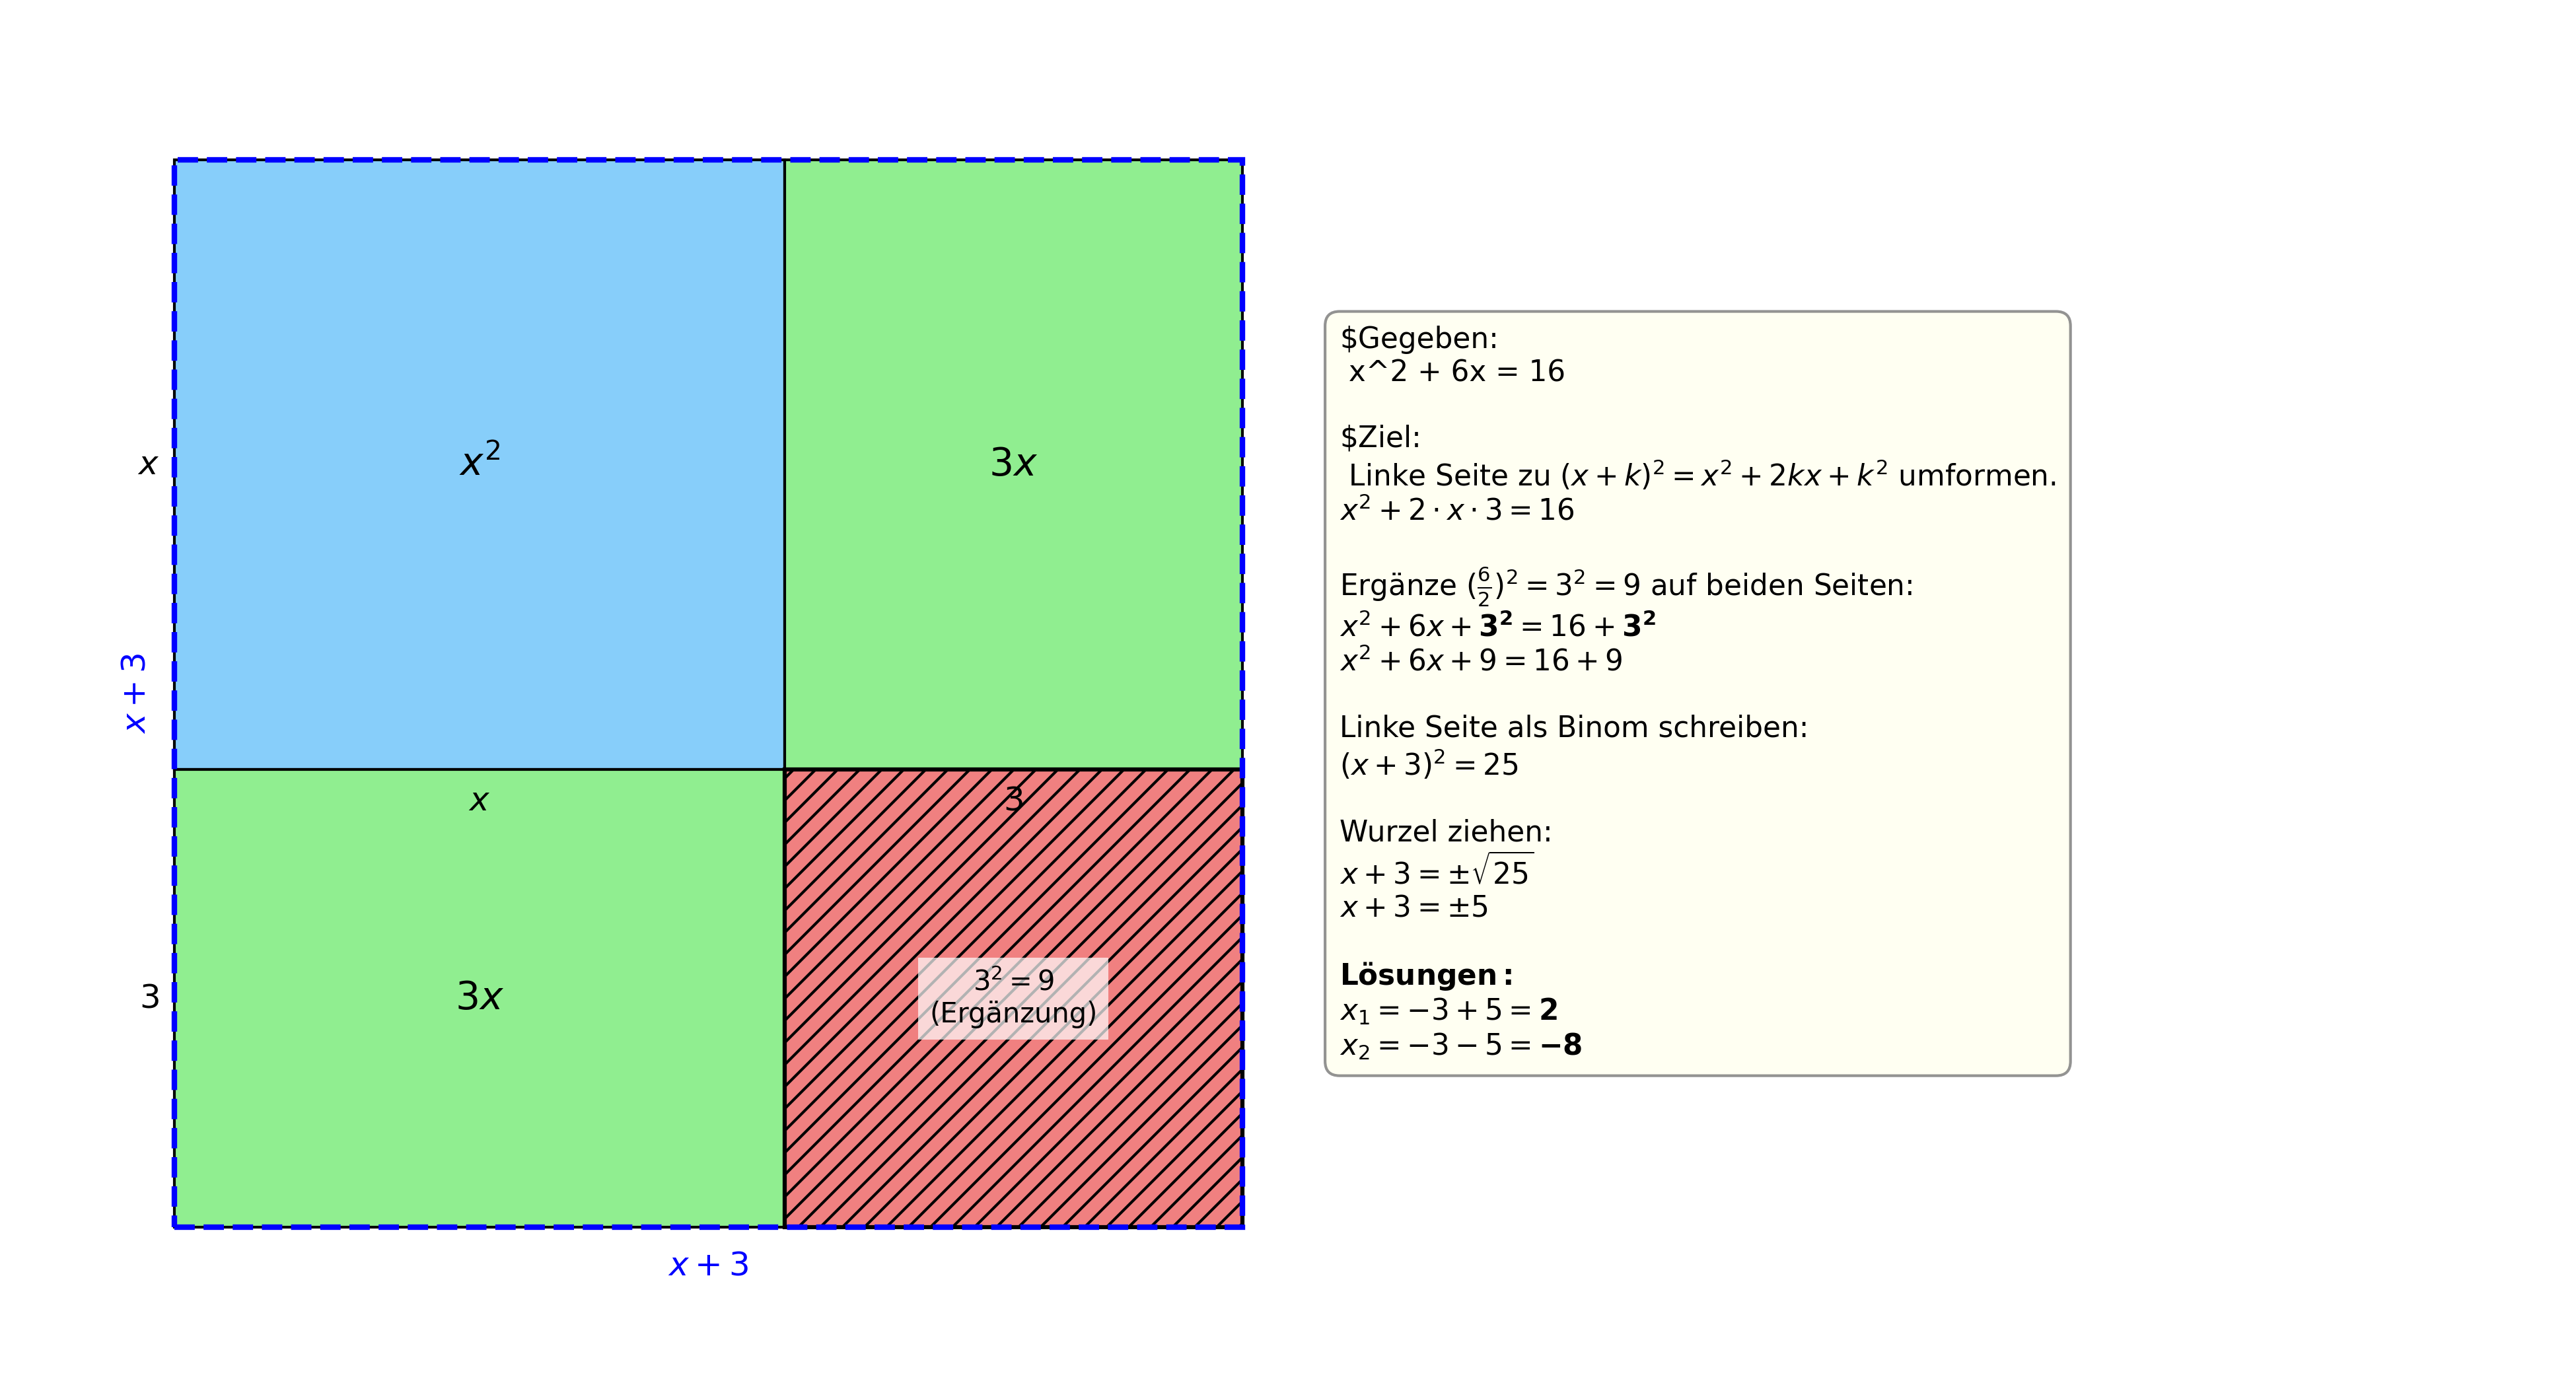
\includegraphics[scale = 0.5]{grafiken/Quadratische_Ergaenzung_Visualisierung.png}
    \captionof{figure}{Grafische Darstellung der quadratischen Ergänzung für $x^2+6x=16$}
    \label{fig:quad_ergaenzung_visual}
\end{center}
% Der Text geht hier direkt weiter


\begin{aufgabenumgebung}{Übung zur quadratischen Ergänzung und Scheitelpunktbestimmung}
Bestimme für die folgenden Funktionen den Scheitelpunkt, indem du die Normalform durch quadratische Ergänzung in die Scheitelpunktform überführst. Gib auch an, ob es sich um ein Maximum oder Minimum handelt.
\begin{enumerate}
    \item $f(x) = x^2 - 6x + 5$
    \item $g(x) = x^2 + 8x + 10$
    \item $h(x) = 2x^2 + 4x - 1$ (Tipp: Erst den Faktor 2 ausklammern!)
    \item $k(x) = -x^2 - 2x + 3$ (Tipp: Erst den Faktor -1 ausklammern!)
\end{enumerate}
Vergleiche deine Ergebnisse für $x_S$ mit der Formel $x_S = -b/(2a)$.
\end{aufgabenumgebung}

\subsection{Symmetrie von Parabeln}
\label{subsec:symmetrie_parabeln}

Eine der auffälligsten Eigenschaften von Parabeln ist ihre Symmetrie. Jede Parabel ist \textbf{achsensymmetrisch}. Das bedeutet, es gibt eine Gerade (die Symmetrieachse), an der man die Parabel spiegeln kann, sodass sie genau auf sich selbst abgebildet wird.

\begin{merksatzumgebung}{Symmetrieachse einer Parabel}
\begin{itemize}
    \item Die Symmetrieachse einer Parabel $f(x)=ax^2+bx+c$ ist immer eine \textbf{senkrechte Gerade}, die durch den \textbf{Scheitelpunkt $S(x_S|y_S)$} verläuft.
    \item Die Gleichung dieser Symmetrieachse lautet daher: \[ x = x_S \] wobei $x_S = -\frac{b}{2a}$ die x-Koordinate des Scheitelpunkts ist.
    \item \textbf{Spezialfall: Symmetrie zur y-Achse}
        Eine Parabel ist genau dann achsensymmetrisch zur y-Achse (deren Gleichung $x=0$ ist), wenn ihre Symmetrieachse $x=x_S$ mit der y-Achse zusammenfällt. Das bedeutet $x_S=0$.
        Setzen wir $x_S = -\frac{b}{2a} = 0$. Da $a \neq 0$ sein muss, kann dieser Ausdruck nur Null werden, wenn der Zähler $b=0$ ist.
        Also: \textbf{Eine Parabel $f(x)=ax^2+bx+c$ ist genau dann achsensymmetrisch zur y-Achse, wenn $b=0$ ist.} Die Funktionsgleichung lautet dann $f(x)=ax^2+c$.
\end{itemize}
\end{merksatzumgebung}

\textbf{Wie testet man rechnerisch auf Achsensymmetrie zur y-Achse?}
Eine Funktion $f(x)$ ist achsensymmetrisch zur y-Achse, wenn für alle $x$ aus dem Definitionsbereich gilt:
\[ f(-x) = f(x) \]
Setzt man also $-x$ in die Funktion ein, muss dasselbe herauskommen, als wenn man $x$ einsetzt.

\begin{beispielumgebung}{Symmetrieuntersuchung}
\textbf{1. Funktion $f(x) = 2x^2 - 3$}
Hier ist $a=2, b=0, c=-3$. Da $b=0$ ist, erwarten wir Achsensymmetrie zur y-Achse.
Test: $f(-x) = 2(-x)^2 - 3 = 2x^2 - 3 = f(x)$.
Die Bedingung ist erfüllt, die Funktion ist achsensymmetrisch zur y-Achse. Der Scheitelpunkt liegt bei $S(0|-3)$.

\textbf{2. Funktion $g(x) = x^2 + 4x + 1$}
Hier ist $a=1, b=4, c=1$. Da $b \neq 0$, ist die Funktion NICHT achsensymmetrisch zur y-Achse.
Test: $g(-x) = (-x)^2 + 4(-x) + 1 = x^2 - 4x + 1$.
Das ist ungleich $g(x) = x^2+4x+1$ (es sei denn $x=0$).
Die Funktion ist aber achsensymmetrisch zu ihrer Symmetrieachse $x=x_S$. Wir hatten berechnet $x_S=-2$. Die Symmetrieachse ist also $x=-2$.
Das bedeutet z.B., dass $g(-1)$ denselben Wert haben muss wie $g(-3)$, da beide Punkte den gleichen Abstand (nämlich 1) von der Symmetrieachse $x=-2$ haben.
$g(-1) = (-1)^2+4(-1)+1 = 1-4+1 = -2$.
$g(-3) = (-3)^2+4(-3)+1 = 9-12+1 = -2$. Stimmt!
\end{beispielumgebung}

\begin{aufgabenumgebung}{Symmetrie prüfen und bestimmen}
\begin{enumerate}
    \item Untersuche die folgenden Funktionen rechnerisch auf Achsensymmetrie zur y-Achse, indem du $f(-x)$ berechnest und mit $f(x)$ vergleichst.
        \begin{itemize}
            \item $f_1(x) = -3x^2 + 5$
            \item $f_2(x) = x^2 - 2x + 1$
            \item $f_3(x) = 4x^2$
        \end{itemize}
    \item Bestimme für die Funktion $f(x) = 0.5x^2 - 3x + 1$ die Gleichung ihrer Symmetrieachse. Überprüfe dann für zwei verschiedene x-Werte, die symmetrisch zu dieser Achse liegen, ob ihre Funktionswerte gleich sind.
\end{enumerate}
\end{aufgabenumgebung}

Ein weiteres wichtiges Merkmal von Funktionen sind ihre Nullstellen.

\subsection{Nullstellen – Wo schneidet die Parabel die x-Achse?}

Nullstellen einer Funktion sind die x-Werte, an denen der Funktionswert $f(x)$ gleich Null ist. Grafisch sind das die \textbf{Schnittpunkte (oder der Berührpunkt) des Graphen mit der x-Achse}.
Eine quadratische Funktion $f(x)=ax^2+bx+c$ kann, wie du vielleicht schon in Skizzen gesehen hast:
\begin{itemize}
    \item \textbf{zwei verschiedene} reelle Nullstellen haben (die Parabel schneidet die x-Achse an zwei Stellen).
    \item \textbf{genau eine} (man sagt auch doppelte) reelle Nullstelle haben (die Parabel berührt die x-Achse genau in ihrem Scheitelpunkt).
    \item \textbf{keine} reelle Nullstelle haben (die Parabel verläuft komplett oberhalb oder komplett unterhalb der x-Achse und schneidet oder berührt sie nie).
\end{itemize}

Um die Nullstellen zu finden, setzen wir den Funktionsterm gleich Null:
$f(x) = 0 \implies ax^2+bx+c=0$.
Dies ist eine \textbf{quadratische Gleichung}, und für ihre Lösung gibt es bekannte Formeln.

\begin{merksatzumgebung}[Nullstellen berechnen mit Lösungsformeln]{Die Mitternachtsformel und die p-q-Formel}
\textbf{1. Die Mitternachtsformel (oft auch ABC-Formel genannt):}
Diese Formel ist universell einsetzbar für jede quadratische Gleichung der Form $ax^2+bx+c=0$ (wobei $a \neq 0$).
Die Lösungen (Nullstellen) $x_1$ und $x_2$ sind gegeben durch:
\[ x_{1,2} = \frac{-b \pm \sqrt{b^2 - 4ac}}{2a} \]
Der Ausdruck unter der Wurzel, $D = b^2 - 4ac$, wird \textbf{Diskriminante} genannt. Das Vorzeichen der Diskriminante entscheidet über die Anzahl der reellen Lösungen (Nullstellen):
\begin{itemize}
    \item $D > 0$: Zwei verschiedene reelle Nullstellen. Die Wurzel $\sqrt{D}$ ist eine positive reelle Zahl.
    \item $D = 0$: Genau eine (doppelte) reelle Nullstelle: $x_1 = x_2 = -\frac{b}{2a}$. (Der Scheitelpunkt liegt auf der x-Achse). Die Wurzel $\sqrt{D}$ ist Null.
    \item $D < 0$: Keine reelle Nullstelle. Man kann im Reellen keine Wurzel aus einer negativen Zahl ziehen. Die Parabel schneidet die x-Achse nicht.
\end{itemize}
\textit{Warum 'Diskriminante'?} Weil sie die Fälle unterscheidet (lat. discriminare = unterscheiden).

\textbf{2. Die p-q-Formel:}
Diese Formel ist eine spezielle Version für quadratische Gleichungen, die bereits in der \textbf{Normalform} $x^2+px+q=0$ vorliegen (d.h., der Koeffizient vor $x^2$ ist 1).
Wenn deine Gleichung $ax^2+bx+c=0$ mit $a \neq 1$ ist, musst du sie zuerst durch $a$ teilen: $x^2 + \frac{b}{a}x + \frac{c}{a} = 0$. Dann ist $p = \frac{b}{a}$ und $q = \frac{c}{a}$.
Die Lösungen (Nullstellen) sind dann:
\[ x_{1,2} = -\frac{p}{2} \pm \sqrt{\left(\frac{p}{2}\right)^2 - q} \]
Auch hier entscheidet der Ausdruck unter der Wurzel, $D_{pq} = \left(\frac{p}{2}\right)^2 - q$ (die Diskriminante der p-q-Formel), über die Anzahl der Nullstellen.

\textbf{Welche Formel soll ich nehmen?}
\begin{itemize}
    \item Die Mitternachtsformel funktioniert immer und du musst nicht vorher durch $a$ teilen.
    \item Die p-q-Formel ist etwas kürzer, wenn die Gleichung schon in der Form $x^2+px+q=0$ ist oder leicht dorthin gebracht werden kann.
\end{itemize}
Wähle die Formel, mit der du dich sicherer fühlst und weniger Fehler machst! Es ist gut, beide zu kennen.
\end{merksatzumgebung}

Machen wir Beispiele für beide Formeln.

\begin{beispielumgebung}[Nullstellen mit Mitternachtsformel]{Nullstellen von $f(x) = 2x^2 - 4x - 6$}
Wir setzen $f(x)=0$: $2x^2 - 4x - 6 = 0$.
Koeffizienten: $a=2$, $b=-4$, $c=-6$.

\textbf{Schritt 1: Diskriminante $D$ berechnen}
$D = b^2 - 4ac = (-4)^2 - 4 \cdot 2 \cdot (-6) = 16 - (-48) = 16 + 48 = 64$.
Da $D=64 > 0$, wissen wir, dass es zwei verschiedene reelle Nullstellen geben wird.

\textbf{Schritt 2: Mitternachtsformel anwenden}
\[ x_{1,2} = \frac{-(-4) \pm \sqrt{64}}{2 \cdot 2} = \frac{4 \pm 8}{4} \]
Die beiden Nullstellen sind:
$x_1 = \frac{4 + 8}{4} = \frac{12}{4} = 3$.
$x_2 = \frac{4 - 8}{4} = \frac{-4}{4} = -1$.
Die Schnittpunkte mit der x-Achse sind also $N_1(3|0)$ und $N_2(-1|0)$.
\end{beispielumgebung}

\begin{beispielumgebung}[Nullstellen mit p-q-Formel]{Nullstellen von $f(x) = x^2 - 6x + 5$}
Wir setzen $f(x)=0$: $x^2 - 6x + 5 = 0$.
Diese Gleichung ist schon in der Normalform $x^2+px+q=0$.
Koeffizienten für die p-q-Formel: $p=-6$ und $q=5$.

\textbf{Schritt 1: Diskriminante $D_{pq}$ der p-q-Formel berechnen}
$D_{pq} = \left(\frac{p}{2}\right)^2 - q = \left(\frac{-6}{2}\right)^2 - 5 = (-3)^2 - 5 = 9 - 5 = 4$.
Da $D_{pq}=4 > 0$, erwarten wir zwei verschiedene reelle Nullstellen.

\textbf{Schritt 2: p-q-Formel anwenden}
$x_{1,2} = -\frac{p}{2} \pm \sqrt{D_{pq}}$
$x_{1,2} = -\frac{-6}{2} \pm \sqrt{4}$
$x_{1,2} = 3 \pm 2$

Die beiden Nullstellen sind:
$x_1 = 3 + 2 = 5$.
$x_2 = 3 - 2 = 1$.
Die Schnittpunkte mit der x-Achse sind $N_1(5|0)$ und $N_2(1|0)$.
\end{beispielumgebung}

Achte immer sorgfältig auf die Vorzeichen, wenn du die Werte für $a,b,c$ oder $p,q$ einsetzt!

\begin{aufgabenumgebung}{Nullstellen finden – Übung und Vertiefung}
Berechne die Nullstellen der folgenden Funktionen. Entscheide selbst, welche Methode (Ausklammern, p-q-Formel, Mitternachtsformel, Substitution) am besten geeignet ist. Überprüfe bei quadratischen Gleichungen immer zuerst die Diskriminante, um die Anzahl der erwarteten reellen Nullstellen zu bestimmen.
\begin{enumerate}
    \item $f(x) = x^2 - x - 6$
        \begin{tippumgebung}{Lösungsweg}
        Dies ist eine Standard-quadratische Gleichung. p-q-Formel oder Mitternachtsformel sind hier gut geeignet.
        \end{tippumgebung}

    \item $g(x) = -2x^2 + 12x - 18$ 
        \begin{tippumgebung}{Besondere Diskriminante}
        Was sagt $D=0$ über den Graphen und die Art der Nullstelle aus?
        \end{tippumgebung}

    \item $h(x) = x^2 + 2x + 5$
        \begin{tippumgebung}{Keine reellen Nullstellen?}
        Was bedeutet es für den Graphen, wenn die Diskriminante $D<0$ ist?
        \end{tippumgebung}

    \item $k(x) = 3x^2 - 12$ 
        \begin{tippumgebung}{Vereinfachung}
        Hier geht es auch ohne Mitternachtsformel! Denke an das direkte Auflösen nach $x^2$. (Siehe Infobox zu Sonderfällen).
        \end{tippumgebung}

    \item $m(x) = -0.5x^2 + 2x$
        \begin{tippumgebung}{Ausklammern}
        Auch hier ist Ausklammern der schnellste Weg! (Siehe Infobox zu Sonderfällen).
        \end{tippumgebung}

    \item \textbf{Polynom 3. Grades durch Ausklammern:}
        $p(x) = x^3 - 5x^2 + 6x$
        \begin{tippumgebung}{Strategie}
        Klammere zuerst den gemeinsamen Faktor $x$ aus. Übrig bleibt ein quadratischer Term, dessen Nullstellen du mit den bekannten Formeln finden kannst.
        \end{tippumgebung}

    \item \textbf{Biquadratische Funktion:}
        $q(x) = x^4 - 10x^2 + 9$
        \begin{tippumgebung}{Substitution}
        Ersetze (substituiere) $x^2$ durch eine neue Variable, z.B. $z = x^2$. Dadurch erhältst du eine quadratische Gleichung in $z$. Löse diese nach $z$ und substituiere dann zurück ($x^2 = z_1$, $x^2 = z_2$), um die Nullstellen für $x$ zu finden. Achtung: Nicht jede Lösung für $z$ führt zu reellen Lösungen für $x$!
        \end{tippumgebung}

    \item \textbf{Produkt aus Linearfaktoren (versteckt):}
        $r(x) = (x^2-4)(x^2+x-2)$
        \begin{tippumgebung}{Satz vom Nullprodukt und Faktorisieren}
        Ein Produkt ist Null, wenn einer der Faktoren Null ist. Setze also jeden Klammerausdruck gleich Null. Der erste Faktor lässt sich mit der 3. binomischen Formel zerlegen. Für den zweiten Faktor kannst du die p-q-Formel verwenden.
        \end{tippumgebung}

    \item \textbf{Funktion mit bekannter Nullstelle (für Knobler):}
        Gegeben ist die Funktion $s(x) = x^3 - 2x^2 - 5x + 6$. Es ist bekannt, dass $x_1=1$ eine Nullstelle ist. Finde die anderen Nullstellen.
        \begin{tippumgebung}{Faktor abspalten}
        Wenn $x_1=1$ eine Nullstelle ist, dann ist $(x-1)$ ein Linearfaktor des Polynoms. Du könntest versuchen, $s(x)$ als $(x-1) \cdot (\text{quadratischer Term})$ zu schreiben.
        Überlege: $(x-1)(ax^2+bx+c) = ax^3 + bx^2 + cx - ax^2 - bx - c = ax^3 + (b-a)x^2 + (c-b)x - c$.
        Vergleiche die Koeffizienten dieses ausmultiplizierten Terms mit den Koeffizienten von $s(x)=1x^3 - 2x^2 - 5x + 6$:
        \begin{itemize}
            \item $a$ muss $1$ sein.
            \item $-c$ muss $6$ sein, also $c=-6$.
            \item $b-a = -2 \implies b-1 = -2 \implies b = -1$.
        \end{itemize}
        Der quadratische Term ist also $(x^2-x-6)$. Finde nun dessen Nullstellen. (Dieses Verfahren nennt man Koeffizientenvergleich und ist eine Alternative zur Polynomdivision, welche wir später kennenlernen, wenn eine Nullstelle bekannt ist).
        \end{tippumgebung}

    \item \textbf{Nullstellen und Parameter:}
        Für welche Werte des Parameters $k$ hat die Funktion $f_k(x) = x^2 - 2kx + (k+2)$ genau eine, zwei oder keine reelle(n) Nullstelle(n)?
        \begin{tippumgebung}{Diskriminante}
        Untersuche die Diskriminante $D = b^2-4ac$ der quadratischen Gleichung $f_k(x)=0$ in Abhängigkeit von $k$.
        Setze $D=0$ für eine Nullstelle, $D>0$ für zwei und $D<0$ für keine.
        \end{tippumgebung}

\end{enumerate}
\end{aufgabenumgebung}

\begin{infoboxumgebung}{Sonderfälle beim Nullstellenfinden – Denk an die Abkürzungen!}
Nicht immer musst du die großen Lösungsformeln bemühen. Für spezielle Formen quadratischer Gleichungen geht es schneller:

\begin{itemize}
    \item \textbf{Fall 1: $c=0$ (der konstante Term fehlt, also $ax^2 + bx = 0$)}
    Hier kannst du immer $x$ ausklammern: $x(ax+b)=0$.
    Ein Produkt ist genau dann Null, wenn einer seiner Faktoren Null ist. Also:
    $x_1 = 0$ \quad ODER \quad $ax+b=0$.
    Die zweite Gleichung $ax+b=0$ löst du einfach nach $x$ auf: $ax = -b \implies x_2 = -\frac{b}{a}$.
    Eine Nullstelle ist also immer $x_1=0$ (die Parabel geht durch den Ursprung), die andere ist $x_2 = -b/a$.
    Beispiel: $f(x) = 2x^2 - 6x$. Nullstellen: $x(2x-6)=0 \implies x_1=0$ oder $2x-6=0 \implies 2x=6 \implies x_2=3$.

    \item \textbf{Fall 2: $b=0$ (der lineare Term $bx$ fehlt, also $ax^2 + c = 0$ – reinquadratische Gleichung)}
    Diese Gleichung kannst du direkt nach $x^2$ auflösen:
    $ax^2 = -c \implies x^2 = -\frac{c}{a}$.
    Dann ziehst du die Wurzel: $x_{1,2} = \pm \sqrt{-\frac{c}{a}}$.
    Diese Gleichung hat reelle Lösungen, wenn der Ausdruck unter der Wurzel (Radikand) nicht-negativ ist, also $-\frac{c}{a} \ge 0$.
    \begin{itemize}
        \item Wenn $-\frac{c}{a} > 0$: zwei Lösungen $x_1 = \sqrt{-\frac{c}{a}}$ und $x_2 = -\sqrt{-\frac{c}{a}}$.
        \item Wenn $-\frac{c}{a} = 0$ (also $c=0$, was uns zu Fall 1 führt, wenn $b$ auch 0 ist, oder $x^2=0$): eine Lösung $x=0$.
        \item Wenn $-\frac{c}{a} < 0$: keine reelle Lösung.
    \end{itemize}
    Beispiel: $f(x) = 2x^2 - 8$. Nullstellen: $2x^2 - 8 = 0 \implies 2x^2 = 8 \implies x^2 = 4 \implies x_{1,2} = \pm 2$.
    Beispiel: $f(x) = x^2 + 1$. Nullstellen: $x^2 + 1 = 0 \implies x^2 = -1$. Keine reellen Lösungen.
\end{itemize}
Halte immer Ausschau nach diesen einfacheren Fällen, bevor du die Mitternachts- oder p-q-Formel anwendest!
\end{infoboxumgebung}

\begin{fehlerboxumgebung}{Typische Fehler bei quadratischen Funktionen}
\begin{itemize}
    \item \textbf{Vorzeichenfehler bei der quadratischen Ergänzung:} Besonders beim Ausklammern eines negativen Faktors $a$ oder beim Auflösen der Klammer.
    \item \textbf{Vorzeichenfehler in der Mitternachts-/p-q-Formel:} Achte genau auf $-b$ oder $-p/2$ und die Zeichen unter der Wurzel.
    \item \textbf{Diskriminante falsch interpretiert:} $D<0$ bedeutet keine *reelle* Nullstelle, nicht unbedingt 'keine Lösung' (es gibt komplexe Lösungen, die hier aber meist nicht relevant sind).
    \item \textbf{Scheitelpunktform $a(x-x_S)^2+y_S$ falsch abgelesen:} $x_S$ hat in der Formel ein Minus, beim Ablesen also 'Vorzeichen umdrehen'. $y_S$ wird direkt übernommen.
    \item \textbf{Vergessen, durch $a$ zu teilen bei der p-q-Formel:} Die p-q-Formel gilt nur für $x^2+px+q=0$.
\end{itemize}
\end{fehlerboxumgebung}

\begin{infoboxumgebung}{Der Satz von Vieta – Eine elegante Beziehung (für Fortgeschrittene)}
Wenn eine quadratische Gleichung in der Normalform $x^2+px+q=0$ zwei Lösungen $x_1$ und $x_2$ hat (also zwei Nullstellen), dann gibt es einen interessanten Zusammenhang zwischen den Lösungen und den Koeffizienten $p$ und $q$:
\begin{itemize}
    \item $x_1 + x_2 = -p$ (Die Summe der Lösungen ist gleich $-p$)
    \item $x_1 \cdot x_2 = q$ (Das Produkt der Lösungen ist gleich $q$)
\end{itemize}
Dieser Satz von Vieta kann nützlich sein:
\begin{itemize}
    \item Um Lösungen zu überprüfen: Wenn du $x_1, x_2$ berechnet hast, kannst du schnell testen, ob ihre Summe $-p$ und ihr Produkt $q$ ergibt.
    \item Um Gleichungen zu 'konstruieren': Wenn du Nullstellen $x_1, x_2$ kennst, kannst du $p=-(x_1+x_2)$ und $q=x_1x_2$ berechnen und so die Gleichung $x^2+px+q=0$ aufstellen.
    \item Manchmal, um Nullstellen durch 'scharfes Hinsehen' zu erraten, wenn $p$ und $q$ ganze Zahlen sind. (Suche zwei Zahlen, deren Produkt $q$ und deren Summe $-p$ ist).
\end{itemize}
Beispiel: $x^2 - 6x + 5 = 0$. Hier ist $p=-6, q=5$.
Wir suchen zwei Zahlen, deren Produkt 5 und deren Summe $-(-6)=6$ ist. Das sind 1 und 5. Also $x_1=1, x_2=5$.
\end{infoboxumgebung}

\begin{aufgabenumgebung}
        \textbf{Anwendung des Satzes von Vieta (Kopfrechnen für Profis):}
        Versuche, die Nullstellen der folgenden quadratischen Funktionen (in Normalform $x^2+px+q=0$) durch 'scharfes Hinsehen' mit dem Satz von Vieta zu finden. Suche also zwei Zahlen $x_1, x_2$, für die gilt: $x_1+x_2 = -p$ und $x_1 \cdot x_2 = q$.
        \begin{enumerate}[label=(\alph*)]
            \item $f(x) = x^2 - 5x + 6$
            \item $g(x) = x^2 - 3x - 4$
            \item $h(x) = x^2 + 7x + 10$
        \end{enumerate}
        \begin{tippumgebung}{Satz von Vieta nutzen}
        Für $f(x) = x^2 - 5x + 6$: Hier ist $p=-5$ und $q=6$. Du suchst also zwei Zahlen, deren Summe $-p = -(-5) = 5$ ist und deren Produkt $q=6$ ist. Welche Zahlen könnten das sein? (Denke an die Teiler von 6).
        \end{tippumgebung}
\end{aufgabenumgebung}

\begin{merksatzumgebung}[label=merksatz:faktorisierte_form_meh]{Die faktorisierte Form (Nullstellenform) quadratischer Funktionen}
Wenn eine quadratische Funktion $f(x)=ax^2+bx+c$ die (nicht notwendigerweise verschiedenen) reellen Nullstellen $x_1$ und $x_2$ besitzt, kann sie auch in der \textbf{faktorisierten Form} (auch Linearfaktorzerlegung oder Nullstellenform genannt) geschrieben werden:
\[ f(x) = a(x-x_1)(x-x_2) \]
\textbf{Warum ist das nützlich?}
\begin{itemize}
    \item Man kann die Nullstellen $x_1$ und $x_2$ direkt ablesen.
    \item Wenn die Nullstellen und ein weiterer Punkt der Parabel gegeben sind, kann man leicht den Öffnungsfaktor $a$ und damit die Funktionsgleichung bestimmen (siehe Aufgabe \ref{A:QuadratischeAnw}, Teil 3).
    \item Sie zeigt, dass eine quadratische Funktion als Produkt zweier linearer Faktoren (mal dem Faktor $a$) dargestellt werden kann.
\end{itemize}
Wenn es nur eine (doppelte) Nullstelle $x_1$ gibt ($D=0$), dann ist $x_1=x_2$, und die Form lautet $f(x)=a(x-x_1)^2$. Das ist dann gleichzeitig die Scheitelpunktform, wobei der Scheitelpunkt auf der x-Achse liegt ($y_S=0$).
Wenn es keine reellen Nullstellen gibt ($D<0$), existiert keine solche reelle Faktorisierung.
\end{merksatzumgebung}

Mit all diesen Werkzeugen – Scheitelpunktbestimmung und Nullstellenberechnung – können wir nun eine vollständige 'Kurvendiskussion' für quadratische Funktionen durchführen.

\subsection{Kurvendiskussion einer quadratischen Funktion – Das volle Programm}

Eine Kurvendiskussion bedeutet, eine Funktion so vollständig wie möglich zu untersuchen, um ihre Eigenschaften und den Verlauf ihres Graphen zu verstehen. Für quadratische Funktionen ist das noch überschaubar, aber die Systematik hilft dir auch bei komplexeren Funktionen.

\begin{merksatzumgebung}[Kurvendiskussion einer quadratischen Funktion]{Checkliste der Untersuchungspunkte}
Eine vollständige Untersuchung (Kurvendiskussion) einer quadratischen Funktion $f(x)=ax^2+bx+c$ umfasst typischerweise die folgenden Punkte:
\begin{enumerate}
    \item \textbf{Grundlegende Eigenschaften und Definitionsbereich $D_f$:}
        \begin{itemize}
            \item Koeffizienten $a, b, c$ identifizieren.
            \item Öffnungsrichtung ($a>0$ nach oben, $a<0$ nach unten).
            \item Form ($|a|>1$ gestreckt, $0<|a|<1$ gestaucht).
            \item Definitionsbereich: Für quadratische Funktionen immer $D_f = \mathbb{R}$ (alle reellen Zahlen sind erlaubt).
        \end{itemize}
    \item \textbf{Symmetrie:}
        \begin{itemize}
            \item Die Parabel ist immer achsensymmetrisch zur senkrechten Geraden $x = x_S$, die durch ihren Scheitelpunkt geht. (Siehe Abschnitt \ref{subsec:symmetrie_parabeln})
            \item Wenn $b=0$ (also $f(x)=ax^2+c$), dann ist $x_S=0$, und die Parabel ist speziell achsensymmetrisch zur y-Achse.
        \end{itemize}
    \item \textbf{Verhalten für $x \to \pm \infty$ (Globalverhalten):} Was passiert mit $f(x)$, wenn $x$ sehr groß positiv oder sehr groß negativ wird?
        \begin{itemize}
            \item Wenn $a>0$: $f(x) \to \infty$ für $x \to \infty$ und $f(x) \to \infty$ für $x \to -\infty$.
            \item Wenn $a<0$: $f(x) \to -\infty$ für $x \to \infty$ und $f(x) \to -\infty$ für $x \to -\infty$.
        \end{itemize}
    \item \textbf{Schnittpunkt mit der y-Achse ($P_y$):}
        Berechne $f(0)$. Der Punkt ist $P_y(0|c)$. (Sehr einfach!)
    \item \textbf{Nullstellen (Schnittpunkte mit der x-Achse, $N_1, N_2$):}
        Setze $f(x)=0$ und löse die quadratische Gleichung $ax^2+bx+c=0$.
        Bestimme die Anzahl der Nullstellen über die Diskriminante.
        Berechne die Nullstellen $x_1, x_2$ (falls vorhanden). Die Punkte sind $N_1(x_1|0)$ und $N_2(x_2|0)$.
    \item \textbf{Scheitelpunkt $S(x_S|y_S)$ (Extrempunkt):}
        Berechne $x_S = -b/(2a)$ und $y_S = f(x_S)$.
        Gib an, ob es ein \textbf{Hochpunkt (Maximum)}, wenn $a<0$, oder ein \textbf{Tiefpunkt (Minimum)}, wenn $a>0$, ist.
    \item \textbf{Wertebereich $W_f$:} Welche y-Werte kann die Funktion annehmen?
        \begin{itemize}
            \item Wenn $a>0$ (Minimum bei $y_S$): $W_f = \{ y \in \mathbb{R} \,|\, y \ge y_S \} = [y_S, \infty)$.
            \item Wenn $a<0$ (Maximum bei $y_S$): $W_f = \{ y \in \mathbb{R} \,|\, y \le y_S \} = (-\infty, y_S]$.
        \end{itemize}
    \item \textbf{Skizze des Graphen:} Zeichne die Parabel unter Verwendung aller berechneten Punkte (y-Achsenabschnitt, Nullstellen, Scheitelpunkt) und Eigenschaften (Öffnung, Symmetrieachse) möglichst genau in ein Koordinatensystem. Eine Wertetabelle kann zusätzlich helfen.
\end{enumerate}
\end{merksatzumgebung}

Das sieht nach einer langen Liste aus, aber viele dieser Punkte sind schnell abgehakt oder ergeben sich direkt aus vorherigen Berechnungen. Wichtig ist die systematische Abarbeitung.

\begin{beispielumgebung}[Kurvendiskussion durchführen]{Vollständige Untersuchung von $f(x) = -x^2 + 2x + 3$}
Gegeben ist die Funktion $f(x) = -x^2 + 2x + 3$.

\begin{enumerate}
    \item \textbf{Grundlegendes und $D_f$:} Koeffizienten: $a=-1, b=2, c=3$.
    Da $a=-1 < 0$, ist die Parabel nach unten geöffnet. Da $|a|=1$, hat sie die normale Öffnungsweite.
    Definitionsbereich: $D_f = \mathbb{R}$.
    \item \textbf{Symmetrie:} Symmetrieachse $x=x_S$. Da $b \neq 0$, nicht symmetrisch zur y-Achse. $x_S$ wird beim Scheitelpunkt berechnet.
    \item \textbf{Verhalten für $x \to \pm \infty$:} Da $a=-1 < 0$:
    $f(x) \to -\infty$ für $x \to \infty$.
    $f(x) \to -\infty$ für $x \to -\infty$.
    \item \textbf{y-Achsenabschnitt $P_y$:} $f(0) = c = 3$. Also $P_y(0|3)$.
    \item \textbf{Nullstellen $N_1, N_2$:} Setze $f(x)=0 \Rightarrow -x^2+2x+3=0$.
    Mitternachtsformel (siehe früheres Beispiel): $x_1 = -1$, $x_2 = 3$.
    Nullstellenpunkte: $N_1(-1|0)$ und $N_2(3|0)$.
    \item \textbf{Scheitelpunkt $S(x_S|y_S)$:}
    $x_S = -\frac{b}{2a} = -\frac{2}{2(-1)} = -\frac{2}{-2} = 1$.
    $y_S = f(1) = -(1)^2 + 2(1) + 3 = -1 + 2 + 3 = 4$.
    Scheitelpunkt $S(1|4)$. Da $a=-1 < 0$, ist dies ein \textbf{Hochpunkt (Maximum)}.
    Die Symmetrieachse ist die Gerade $x=1$.
    \item \textbf{Wertebereich $W_f$:} Da Hochpunkt bei $y_S=4$ und nach unten geöffnet: $W_f = (-\infty, 4]$.
    \item \textbf{Skizze des Graphen:}
\begin{center}
    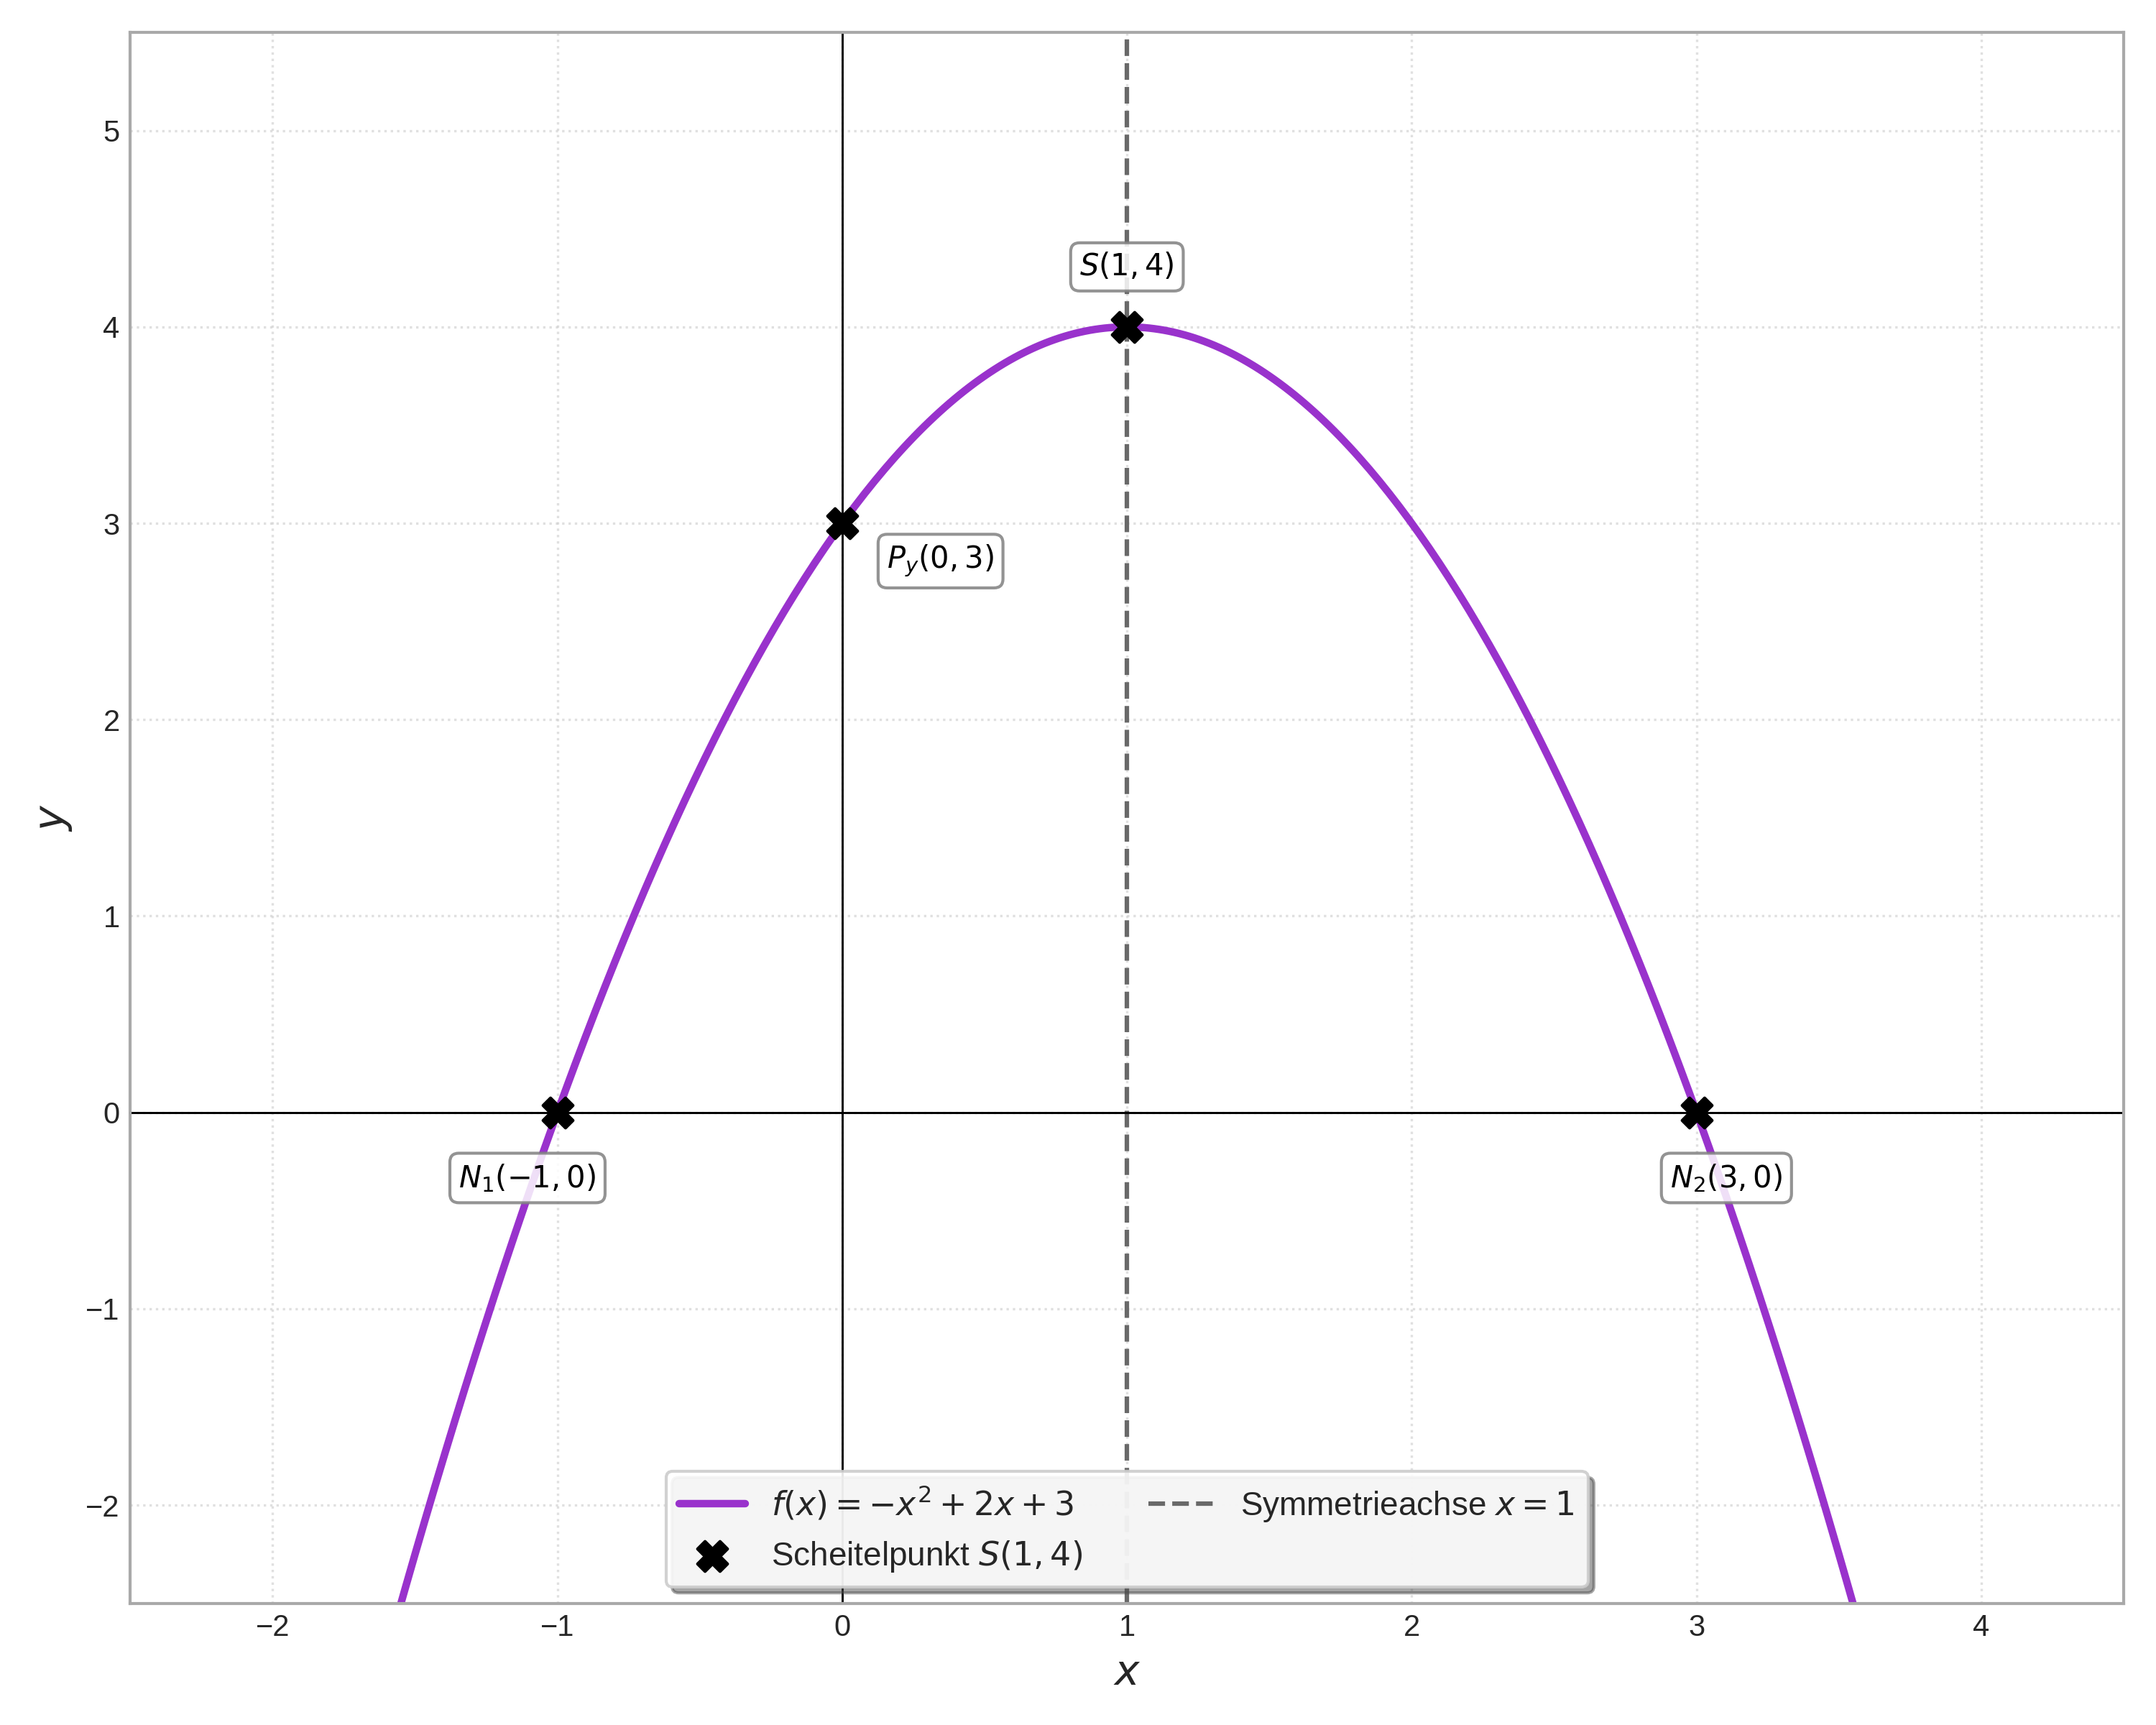
\includegraphics[width=0.9\textwidth]{grafiken/Quadratische_Kurvendiskussion_Beispiel.png}
    \captionof{figure}{Graph der Funktion $f(x)=-x^2+2x+3$ mit wichtigen Punkten}
    \label{fig:kurvendisk_beispiel}
\end{center}
\end{enumerate}
\end{beispielumgebung}

Eine vollständige Kurvendiskussion gibt dir ein sehr gutes Bild von der Funktion.

\begin{aufgabenumgebung}{Deine Kurvendiskussion – Quadratische Funktionen}
Führe eine vollständige Kurvendiskussion (gemäß der obigen Checkliste) für die folgenden quadratischen Funktionen durch und skizziere jeweils den Graphen.
\begin{enumerate}
    \item $f(x) = x^2 - 4x + 3$
    \item $g(x) = -2x^2 + 8x - 6$
    \item $h(x) = x^2 + 2x + 2$ (Was ist hier bei den Nullstellen und dem Scheitelpunkt besonders?)
    \item $k(x) = x^2 - 2x + 3$ (Untersuche, ob diese Funktion Nullstellen besitzt. Wie wirkt sich das auf den Graphen und den Wertebereich aus?)
    \item $m(x) = -x^2 - 3x + 4$ (Achte auf die Vorzeichen bei der Berechnung des Scheitelpunkts und der Nullstellen.)
\end{enumerate}
\end{aufgabenumgebung}

\subsection{Anwendungsaufgaben mit quadratischen Funktionen – Modellieren und Optimieren}

Quadratische Funktionen sind extrem nützlich, um reale Probleme zu modellieren, besonders wenn es um Flugbahnen, Flächen oder Optimierungsaufgaben (Suche nach Maxima oder Minima) geht.

\begin{aufgabenumgebung}[Brückenbogen]{Der Brückenbogen – eine klassische Anwendung}
Ein parabelförmiger Brückenbogen wird durch eine quadratische Funktion $f(x)$ beschrieben. Der Ursprung des Koordinatensystems $(0|0)$ liegt direkt unter der Mitte des Bogens auf Wasserniveau (x-Achse).
Der Bogen beginnt und endet auf Wasserniveau bei $x=-20\,$m und $x=20\,$m. In der Mitte (also bei $x=0$) ist der Bogen $8\,$m hoch.
\begin{enumerate}
    \item \textbf{Informationen sammeln:} Welche drei Punkte des Graphen der Funktion $f(x)$ sind dir damit bekannt? Notiere ihre Koordinaten.
    \item \textbf{Funktionsgleichung bestimmen:}
        \begin{itemize}
            \item Da der Scheitelpunkt offensichtlich auf der y-Achse liegt (genau in der Mitte bei $x=0$), welche Form hat die quadratische Funktion dann? (Tipp: Welcher Koeffizient ist Null?)
            \item Nutze den Punkt $(0|8)$, um den Koeffizienten $c$ zu bestimmen.
            \item Nutze einen der anderen Punkte (z.B. $(20|0)$), um den Koeffizienten $a$ zu bestimmen.
            \item Schreibe die vollständige Funktionsgleichung $f(x)$ des Brückenbogens auf.
        \end{itemize}
    \item \textbf{Anwendung der Funktion:} Wie hoch ist der Brückenbogen an der Stelle $x=10\,$m vom Mittelpunkt aus gemessen?
    \item \textbf{Skizze:} Erstelle eine Skizze des Brückenbogens im Koordinatensystem.
\end{enumerate}
\begin{center}
    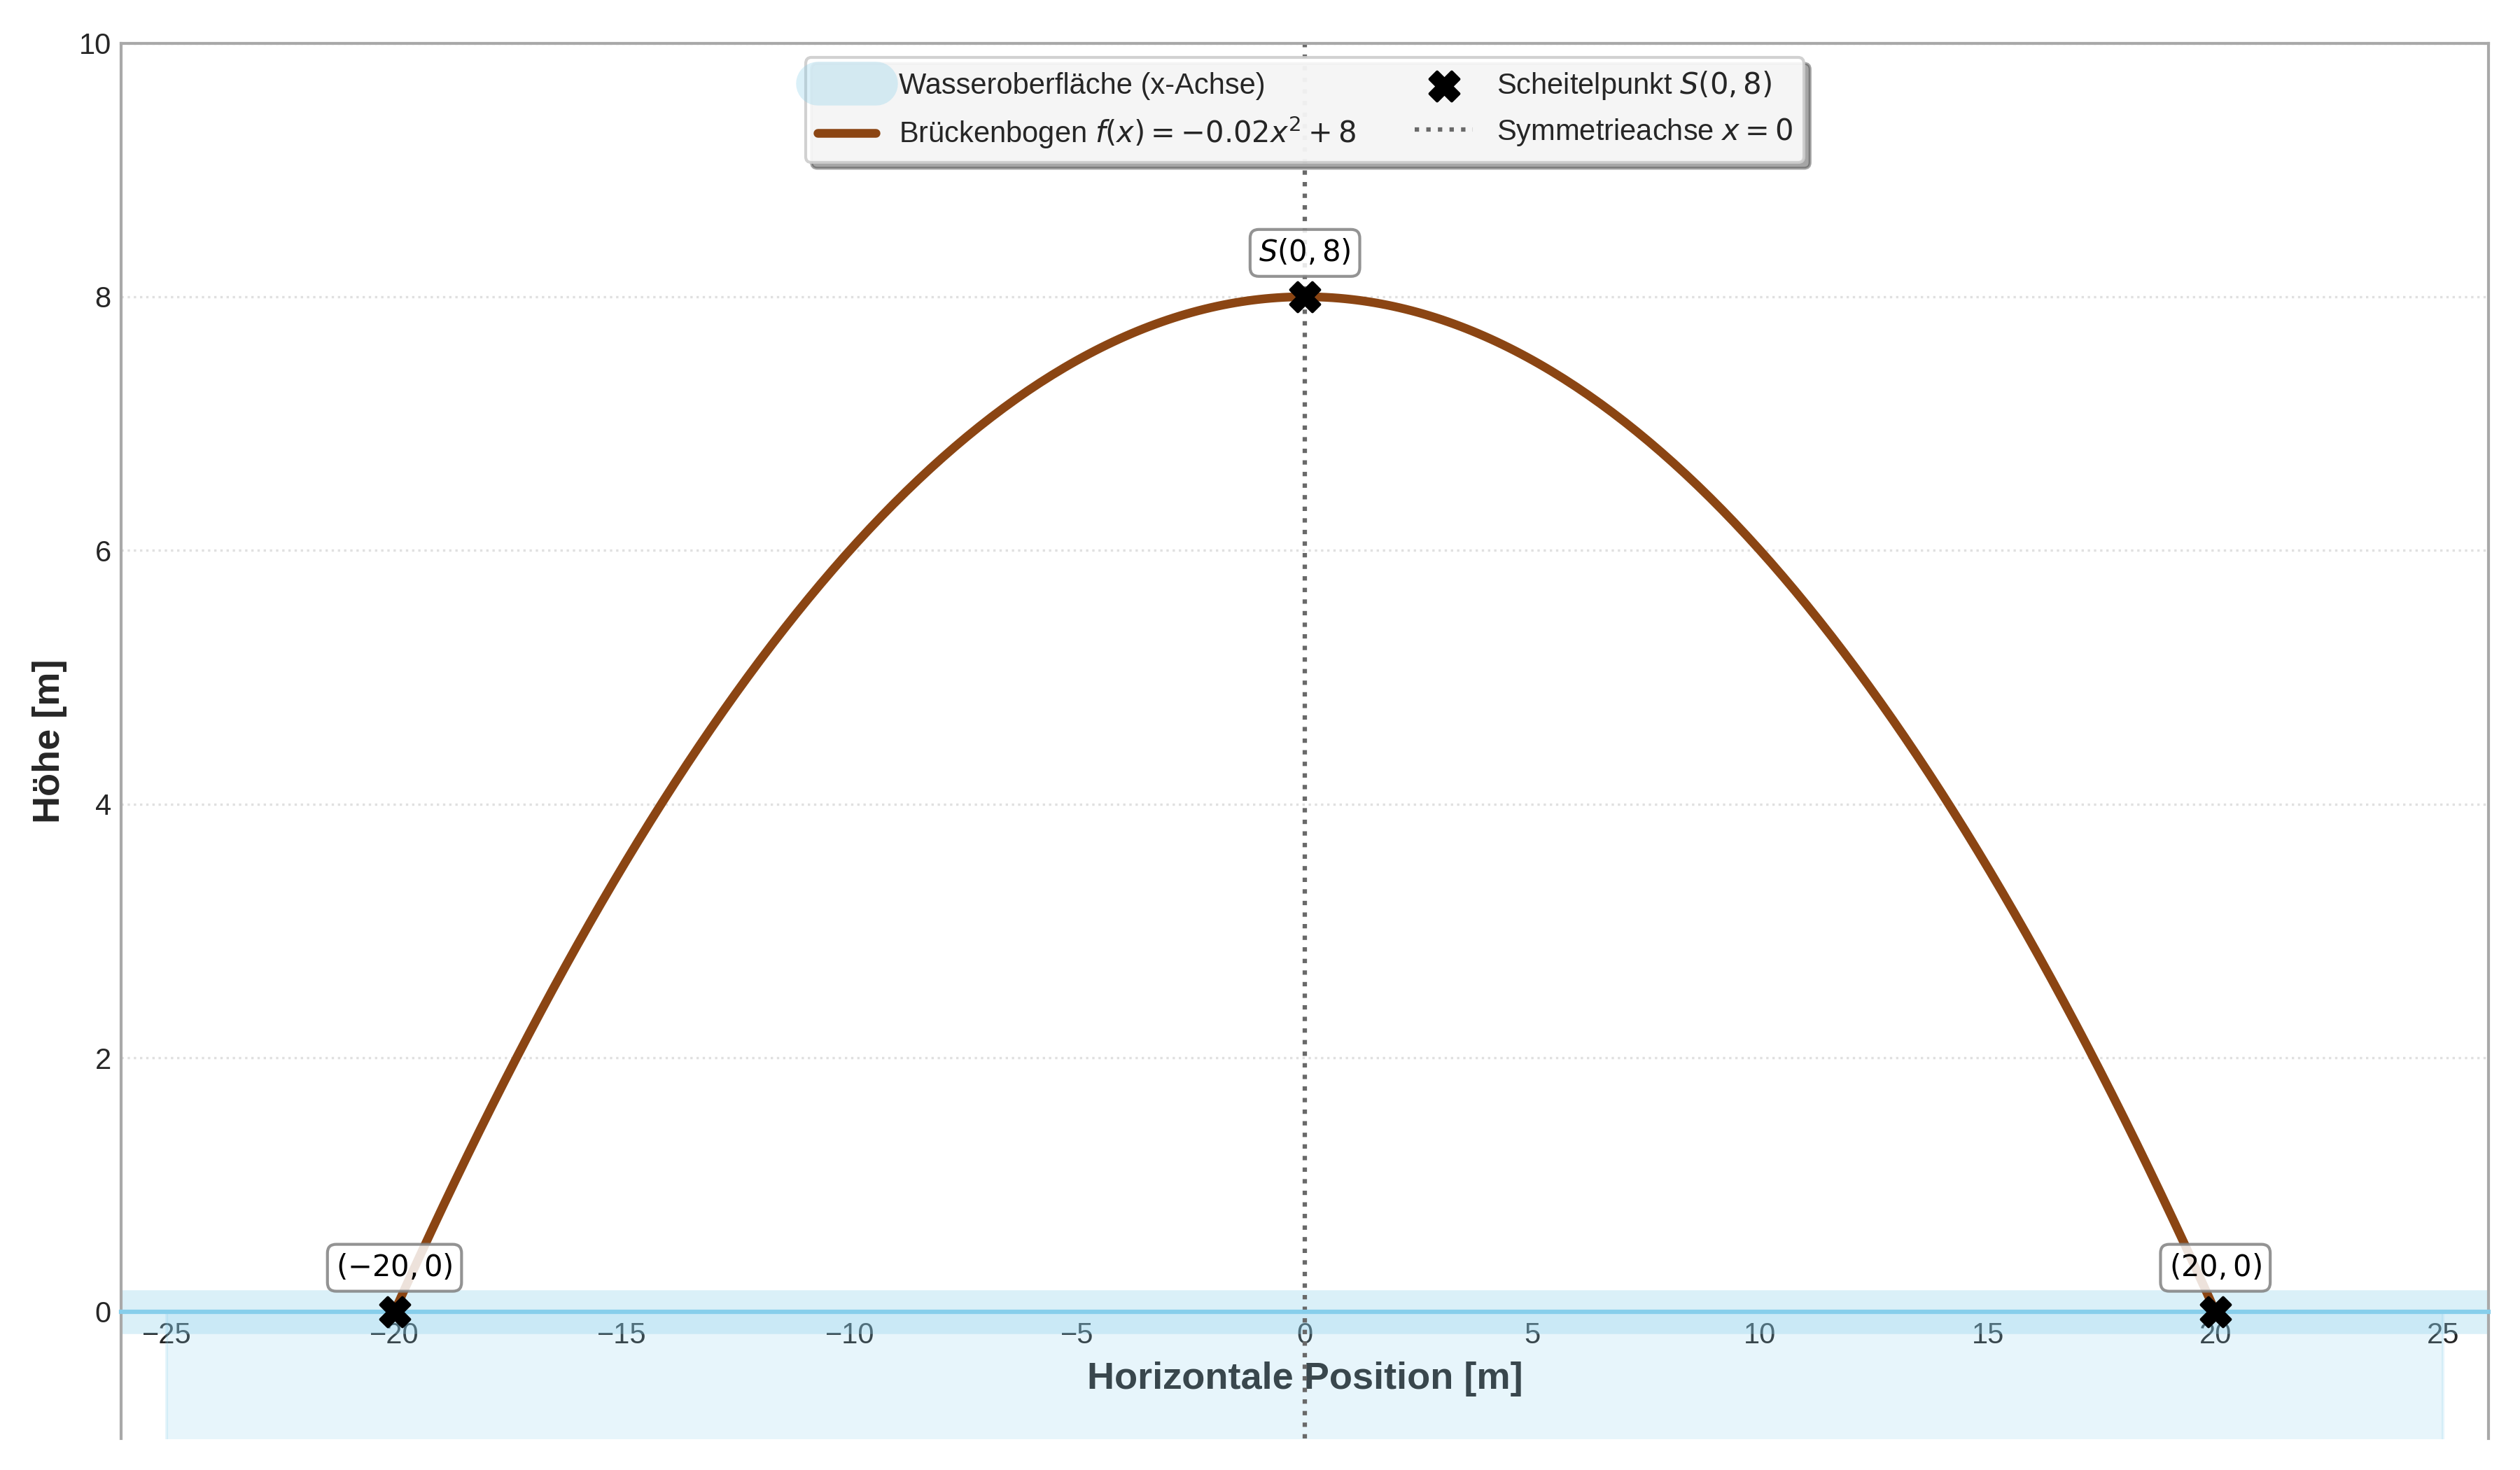
\includegraphics[width=0.7\textwidth]{grafiken/Brueckenbogen_Parabel.png}
    \captionof{figure}{Skizze eines parabelförmigen Brückenbogens}
    \label{fig:brueckenbogen}
\end{center}
\end{aufgabenumgebung}

Eine weitere typische Anwendung ist die Beschreibung von Flugbahnen.

\begin{aufgabenumgebung}{Flugbahn eines Balls}
Ein Ball wird schräg nach oben geworfen. Seine Flughöhe $h(x)$ in Metern über dem Boden kann in Abhängigkeit von der horizontalen Entfernung $x$ (in Metern vom Abwurfpunkt) durch die Funktion
\[ h(x) = -0.1x^2 + 1.2x + 1.6 \]
beschrieben werden (für $x \ge 0$ und solange $h(x) \ge 0$).
\begin{enumerate}
    \item \textbf{Abwurfhöhe:} Aus welcher Höhe wurde der Ball abgeworfen? (Tipp: Das ist die Höhe an der Stelle $x=0$.)
    \item \textbf{Maximale Flughöhe:} Berechne die maximale Flughöhe des Balls. (Tipp: Das ist die y-Koordinate des Scheitelpunkts.)
    \item \textbf{Horizontale Entfernung bei max. Höhe:} Bei welcher horizontalen Entfernung vom Abwurfpunkt erreicht der Ball seine maximale Höhe? (Tipp: Das ist die x-Koordinate des Scheitelpunkts.)
    \item \textbf{Wurfweite:} Bei welcher horizontalen Entfernung trifft der Ball wieder auf dem Boden auf? (Tipp: Gesucht ist die positive Nullstelle der Funktion, da $h(x)=0$ bedeutet, dass der Ball auf dem Boden ist.)
    \item \textbf{Skizze:} Skizziere die Flugbahn des Balls (den Graphen von $h(x)$ im relevanten Bereich). Markiere Abwurfpunkt, höchsten Punkt und Auftreffpunkt.
\end{enumerate}
\end{aufgabenumgebung}

\begin{aufgabenumgebung}[labelA:QuadratischeAnw]{Weitere Anwendungs- und Verständnisaufgaben}
\begin{enumerate}
    \item \textbf{Rechteck mit maximaler Fläche:} Ein Bauer hat 40 Meter Zaun und möchte damit ein rechteckiges Feld an einer langen, geraden Mauer abgrenzen. Die Seite an der Mauer braucht keinen Zaun. Welche Abmessungen (Länge und Breite) sollte das Feld haben, damit seine Fläche maximal wird?
        \begin{itemize}
            \item Sei $x$ die Länge der Seite, die senkrecht zur Mauer steht. Drücke die andere Zaunseite (parallel zur Mauer) ebenfalls durch $x$ aus (bedenke die 40m Gesamtzaunlänge).
            \item Stelle eine Funktion $A(x)$ für die Fläche des Rechtecks in Abhängigkeit von $x$ auf.
            \item Bestimme den Scheitelpunkt dieser quadratischen Funktion $A(x)$. Was bedeuten die Koordinaten des Scheitelpunkts für das Problem?
            \item Gib die optimalen Abmessungen und die maximale Fläche an.
        \end{itemize}
    \item \textbf{Funktion aus Scheitelpunkt und Punkt finden:} Eine Parabel hat ihren Scheitelpunkt bei $S(2|-1)$ und geht durch den Punkt $P(4|7)$. Bestimme ihre Funktionsgleichung. (Tipp: Setze den Scheitelpunkt in die Scheitelpunktform $f(x)=a(x-x_S)^2+y_S$ ein. Setze dann die Koordinaten von $P$ ein, um $a$ zu berechnen.)
    \item \textbf{Funktion aus Nullstellen und Punkt finden:} Eine Parabel schneidet die x-Achse bei $x_1=-1$ und $x_2=3$. Außerdem geht sie durch den Punkt $P(1|-4)$. Bestimme ihre Funktionsgleichung. (Tipp: Nutze die faktorisierte Form einer quadratischen Funktion: $f(x)=a(x-x_1)(x-x_2)$, die wir im Merksatz \ref{merksatz:faktorisierte_form} kennengelernt haben. Setze die Nullstellen ein und dann den Punkt $P$, um $a$ zu berechnen.)
    \item \textbf{Parameter untersuchen:} Gegeben ist die Funktionenschar $f_k(x) = x^2 - 2kx + 4$ mit dem Parameter $k \in \mathbb{R}$.
        \begin{itemize}
            \item Bestimme die Koordinaten des Scheitelpunkts in Abhängigkeit von $k$.
            \item Für welche Werte von $k$ hat die Funktion genau eine Nullstelle? Keine Nullstellen? Zwei Nullstellen? (Tipp: Untersuche die Diskriminante $D$ in Abhängigkeit von $k$.)
            \item Auf welcher Kurve liegen alle Scheitelpunkte der Schar $f_k(x)$? (Tipp: Drücke $y_S$ durch $x_S$ aus. Diese Kurve nennt man auch \textit{Ortskurve} der Scheitelpunkte.)
        \end{itemize}
\end{enumerate}
\end{aufgabenumgebung}

\begin{kurzknappumgebung}{Quadratische Funktionen}
\begin{itemize}
    \item \textbf{Formen:} Normalform $ax^2+bx+c$; Scheitelpunktform $a(x-x_S)^2+y_S$; Faktorisierte Form $a(x-x_1)(x-x_2)$.
    \item \textbf{Graph:} Parabel, Öffnung durch Vorzeichen von $a$, Breite durch Betrag von $a$.
    \item \textbf{Scheitelpunkt $S(x_S|y_S)$:} Extremwert (Max/Min). $x_S = -b/(2a)$, $y_S=f(x_S)$.
    \item \textbf{Symmetrie:} Achsensymmetrisch zu $x=x_S$. Symmetrisch zur y-Achse, wenn $b=0$.
    \item \textbf{Nullstellen:} Schnittpunkte mit x-Achse, Lösung von $ax^2+bx+c=0$ (Mitternachts-/p-q-Formel). Anzahl durch Diskriminante $D=b^2-4ac$.
    \item \textbf{y-Achsenabschnitt:} Bei $(0|c)$.
\end{itemize}
\end{kurzknappumgebung}

\begin{infoboxumgebung}{Ausblick: Mehr als nur Parabeln}
Quadratische Funktionen sind Polynomfunktionen zweiten Grades. Es gibt natürlich auch Polynomfunktionen höheren Grades (kubische Funktionen mit $x^3$, quartische Funktionen mit $x^4$ usw.), die komplexere Kurvenverläufe haben können. Die Werkzeuge, die du hier für quadratische Funktionen lernst (Scheitelpunkt, Nullstellen, Symmetrie), sind oft auch erste Schritte zur Analyse dieser komplizierteren Funktionen, ergänzt durch die Methoden der Differentialrechnung.
\end{infoboxumgebung}

\begin{aufgabenumgebung}{Checkliste: Parabeln verstehen – Mehr als nur Formeln}
Diese Aufgabe soll dir helfen, dein qualitatives Verständnis für quadratische Funktionen und ihre Graphen (Parabeln) zu vertiefen. Oft kann man schon viel über eine Parabel aussagen, ohne gleich jede Formel parat haben zu müssen! Nutze für deine Argumentationen auch immer kleine Skizzen.

\begin{enumerate}[label=\textbf{Teil \arabic*:}]
    \item \textbf{Argumentieren mit Nullstellen und dem Öffnungsfaktor $a$} \\
    Stell dir vor, du kennst von einer quadratischen Funktion $f(x)=ax^2+bx+c$ die Nullstellen (also die $x$-Werte, an denen $f(x)=0$ ist) und das Vorzeichen des Parameters $a$.

    \begin{enumerate}[label=(\alph*)]
        \item Eine Parabel hat die Nullstellen $x_1 = -1$ und $x_2 = 5$. Der Öffnungsfaktor ist $a > 0$.
        \begin{itemize}
            \item Skizziere diese Parabel grob. Ist sie nach oben oder nach unten geöffnet?
            \item In welchen $x$-Bereichen (Intervallen) verlaufen die Funktionswerte $f(x)$ oberhalb der x-Achse (sind also positiv)? In welchen Bereichen verlaufen sie unterhalb (sind also negativ)? Begründe mit deiner Skizze.
            \item Ohne den Scheitelpunkt genau zu berechnen: Was kannst du über die Lage seiner x-Koordinate $x_S$ sagen? (Tipp: Symmetrie!)
        \end{itemize}
        \item Betrachte nun eine andere Parabel mit denselben Nullstellen $x_1 = -1$ und $x_2 = 5$, aber diesmal mit einem Öffnungsfaktor $a < 0$.
        \begin{itemize}
            \item Skizziere auch diesen Fall. Wie ändern sich die Antworten auf die Fragen aus (a) bezüglich Öffnung und Vorzeichen der Funktionswerte?
        \end{itemize}
    \end{enumerate}

    \item \textbf{Argumentieren mit dem y-Achsenabschnitt $c$ und dem Öffnungsfaktor $a$ (Nullstellen sind unbekannt)} \\
    Stell dir vor, du kennst von einer quadratischen Funktion $f(x)=ax^2+bx+c$ nur den y-Achsenabschnitt $c$ (also den Wert $f(0)$) und das Vorzeichen des Öffnungsfaktors $a$.

    \begin{enumerate}[label=(\alph*)]
        \item Eine Parabel ist nach oben geöffnet ($a > 0$) und schneidet die y-Achse bei $c = -2$.
        \begin{itemize}
            \item Skizziere zwei \textit{mögliche} Verläufe für diese Parabel.
            \item Muss diese Parabel zwangsläufig Nullstellen besitzen? Begründe deine Antwort (denke an die Lage des Scheitelpunkts).
            \item Was kannst du über den y-Wert des Scheitelpunkts $y_S$ im Vergleich zum y-Achsenabschnitt $c$ sagen? Ist $y_S \leq c$, $y_S \geq c$ oder kann das variieren? Begründe.
        \end{itemize}
        \item Eine Parabel ist nach unten geöffnet ($a < 0$) und schneidet die y-Achse bei $c = 3$.
        \begin{itemize}
            \item Skizziere auch hier zwei \textit{mögliche} Verläufe.
            \item Kannst du mit Sicherheit sagen, ob diese Parabel Nullstellen hat? Oder ob sie keine hat? Oder ist beides möglich? Erkläre deine Überlegungen.
        \end{itemize}
        \item Eine Parabel ist nach oben geöffnet ($a > 0$) und ihr y-Achsenabschnitt $c$ ist ebenfalls positiv ($c > 0$, z.B. $c=4$).
        \begin{itemize}
            \item Beschreibe und skizziere die drei Möglichkeiten für die Anzahl der Nullstellen (keine, eine, zwei).
            \item Welche Bedingung muss für den Scheitelpunkt (insbesondere dessen y-Koordinate $y_S$) erfüllt sein, damit die Parabel in diesem Fall
            \begin{itemize}
                \item keine Nullstellen hat?
                \item genau eine Nullstelle hat?
                \item zwei Nullstellen hat?
            \end{itemize}
        \end{itemize}
    \end{enumerate}
\end{enumerate}
Versuche, deine Antworten immer auch mit kleinen, beschrifteten Skizzen zu untermauern!
\end{aufgabenumgebung}

\begin{warumwichtigumgebung}{Grundlegendes Verständnis für später}
Ein tiefes Verständnis dafür, wie sich Parameter (wie $a$ und $c$) und besondere Punkte (wie Nullstellen und Scheitelpunkte) auf das Aussehen und Verhalten von linearen und quadratischen Funktionen auswirken, ist nicht nur für diese Funktionstypen selbst wichtig. Dieses Wissen bildet eine entscheidende Grundlage für die Untersuchung komplexerer Funktionen, wie zum Beispiel $f(x)=x^3-2x^2-5x+6$ oder auch $g(x)=(x-1)^4+2$. Auch dort wirst du oft auf lineare oder quadratische Zusammenhänge stoßen, wenn du bestimmte Eigenschaften dieser komplexeren Funktionen analysierst. Ein gutes Fundament hier erleichtert dir also den Zugang zu vielen weiteren spannenden Themen der Analysis! \smiley{}
\end{warumwichtigumgebung}








\subsection{Ein erster Blick auf Polynomfunktionen höheren Grades}
\label{sec:polynome_n_ten_grades}

Lineare (Polynome 1. Grades) und quadratische Funktionen (Polynome 2. Grades) haben uns bereits gezeigt, wie nützlich Funktionen zur Beschreibung von Zusammenhängen sein können – von einfachen Kostenverläufen bis hin zu komplexen Flugbahnen. Doch was, wenn Situationen noch vielschichtiger werden? Hier kommen \textbf{Polynomfunktionen $n$-ten Grades} ins Spiel. Sie sind eine natürliche Erweiterung dessen, was du bereits kennst, und erlauben uns, noch eine größere Vielfalt an Kurven und damit an Phänomenen mathematisch zu erfassen. Lassen wir uns diese genauer ansehen!


Eine Polynomfunktion $n$-ten Grades hat die allgemeine Form:
\[ f(x) = a_n x^n + a_{n-1} x^{n-1} + \dots + a_2 x^2 + a_1 x + a_0 \]
Dabei sind $a_n, a_{n-1}, \dots, a_0$ reelle Zahlen, die man Koeffizienten nennt. Der höchste Exponent $n$ (eine natürliche Zahl) bestimmt den \textbf{Grad} des Polynoms, und der Koeffizient $a_n$ darf nicht Null sein ($a_n \neq 0$).

Lineare Funktionen ($f(x)=a_1x+a_0$) und quadratische Funktionen ($f(x)=a_2x^2+a_1x+a_0$) sind also die einfachsten Vertreter dieser großen Funktionsfamilie. Doch wie sehen Graphen von Polynomen mit einem Grad größer als 2 aus? Sie können deutlich komplexere Formen mit mehr Kurven, 'Bergen' und 'Tälern' aufweisen.

\begin{center} % Geändert von figure-Umgebung zu center-Umgebung
    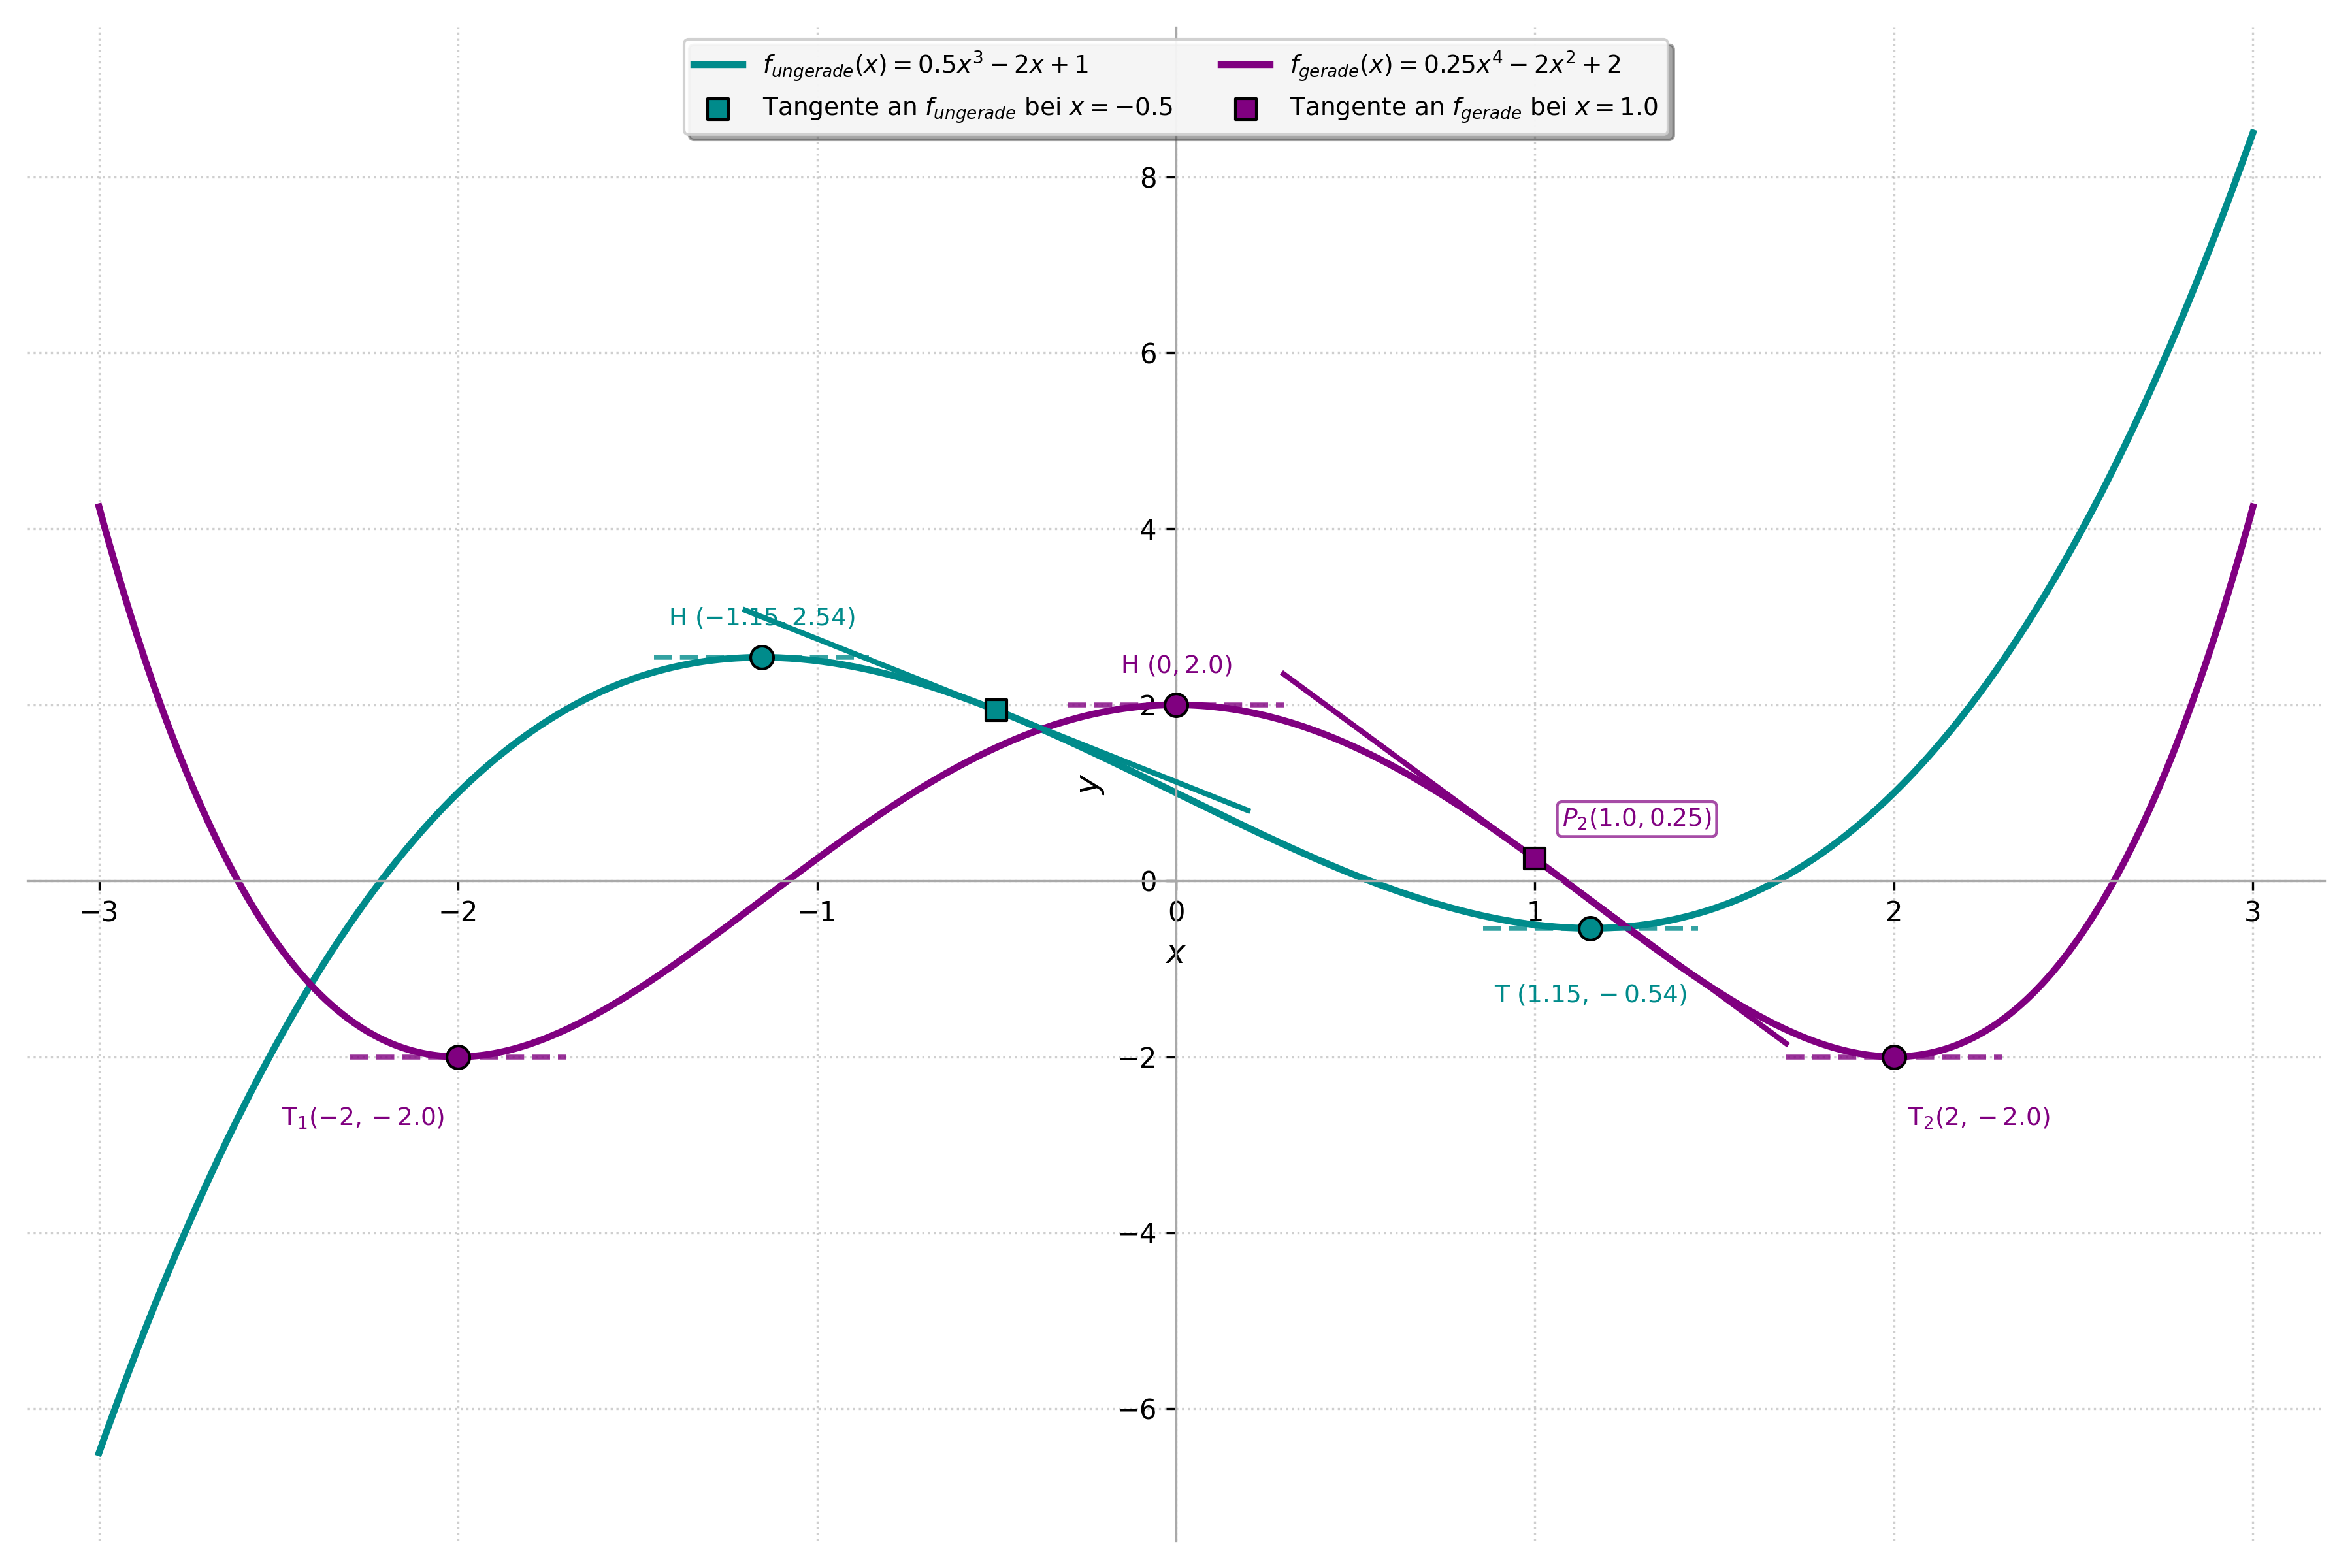
\includegraphics[width=0.9\textwidth]{grafiken/Polynome_Gerade_Ungerade.png}
    \captionof{figure}{Beispiele für Graphen von Polynomfunktionen höheren Grades: ein Polynom 3. Grades (ungerade, in Türkis) und ein Polynom 4. Grades (gerade, in Lila) in einem Koordinatensystem, jeweils mit angedeuteten waagerechten und zusätzlichen nicht-horizontalen Tangenten.}
    \label{fig:polynome_hoeheren_grades}
\end{center}

Wenn du dir die Graphen in Abbildung \ref{fig:polynome_hoeheren_grades} ansiehst, erkennen wir interessante Verläufe und besondere Punkte:

Betrachten wir zuerst die türkisfarbene Kurve, den Graphen der Funktion \textbf{$f_{\text{ungerade}}(x) = 0.5x^3 - 2x + 1$} (ein Polynom 3. Grades).
\begin{itemize}
    \item Wenn wir von links kommen (sehr kleine $x$-Werte), \textbf{steigt} der Graph an, bis er einen lokalen Hochpunkt $H(-1.15 | 2.54)$ erreicht. Man sagt auch, die Funktion ist in diesem Bereich steigend.
    \item Nach diesem Hochpunkt beginnt der Graph zu \textbf{fallen} (die Funktion ist fallend), bis er einen lokalen Tiefpunkt $P_t(1.15 | -0.54)$ erreicht.
    \item Von diesem Tiefpunkt aus \textbf{steigt} der Graph dann wieder an für größere $x$-Werte.
\end{itemize}
An dem Punkt $H$, wo der Graph vom Steigen ins Fallen übergeht, und am Punkt $P_t$, wo er vom Fallen ins Steigen übergeht, muss etwas Besonderes mit der Steigung passieren. Stell dir vor, du fährst mit einem Fahrrad diese Kurve entlang: Um von einer Bergauffahrt in eine Bergabfahrt zu wechseln (oder umgekehrt), musst du für einen winzigen Moment an der Kuppe (oder in der Talsohle) eine Steigung von Null haben – du bist für einen Augenblick waagerecht.\\

Nun zur lilafarbenen Kurve, dem Graphen von \textbf{$f_{\text{gerade}}(x) = 0.25x^4 - 2x^2 + 2$} (ein Polynom 4. Grades).
\begin{itemize}
    \item Dieser Graph \textbf{fällt} von links kommend bis zum lokalen Tiefpunkt $T_1(-2 | -2)$.
    \item Dann \textbf{steigt} er an bis zum lokalen Hochpunkt $H(0 | 2)$.
    \item Anschließend \textbf{fällt} er wieder bis zum lokalen Tiefpunkt $T_2(2 | -2)$.
    \item Und schließlich \textbf{steigt} er für größere $x$-Werte wieder an.
\end{itemize}
Auch hier gilt: An jedem dieser lokalen Hoch- und Tiefpunkte ($T_1, H, T_2$) findet ein Wechsel von Steigen zu Fallen oder von Fallen zu Steigen statt. Intuitiv ist klar, dass die Steigung an diesen Umkehrpunkten genau Null sein muss. Der Graph verläuft dort für einen infinitesimal (also einen gedanklich unendlich kleinen, aber von Null verschiedenen) kleinen Moment waagerecht.

Diese lokalen Hochpunkte (manchmal auch Maxima genannt) und Tiefpunkte (Minima genannt) sind oft die interessantesten Punkte eines Funktionsgraphen.

\begin{infoboxumgebung}{Eine wichtige Beobachtung: Waagerechte Tangenten}
Stell dir vor, du legst an einen solchen lokalen Hoch- oder Tiefpunkt eine Gerade an, die den Graphen an dieser Stelle 'sanft berührt', ohne ihn zu schneiden. Solch eine Gerade nennt man eine \textbf{Tangente} an den Graphen.

Wenn du dir die Tangenten an den Spitzen der 'Berge' und in den 'Tälern' der Polynomgraphen in Abbildung \ref{fig:polynome_hoeheren_grades} vorstellst (angedeutet durch die kurzen waagerechten Linien an den Punkten H, $P_t$, $T_1$ und $T_2$), wirst du feststellen:
\begin{itemize}
    \item Diese Tangenten scheinen \textbf{waagerecht} zu verlaufen.
    \item Eine waagerechte Gerade hat aber die \textbf{Steigung Null}!
\end{itemize}
Diese Beobachtung – dass an lokalen Hoch- und Tiefpunkten die Steigung der Tangente Null zu sein scheint – ist ein extrem wichtiges Konzept in der Mathematik. Es gibt uns einen ersten Hinweis darauf, wie wir solche besonderen Punkte später, mit den Methoden der Differentialrechnung, auch rechnerisch exakt finden können. Behalte diese Idee im Hinterkopf!
\end{infoboxumgebung}

Obwohl wir Polynomfunktionen höheren Grades hier nicht so detailliert untersuchen wie lineare oder quadratische Funktionen (dafür fehlen uns noch einige Werkzeuge), ist es gut zu wissen, dass sie existieren und dass die Konzepte von Steigung und besonderen Punkten auch bei ihnen eine zentrale Rolle spielen werden. Die Fähigkeit, Graphen zu interpretieren und Besonderheiten zu erkennen, wird dir auf deinem weiteren Weg in der Analysis sehr helfen. \\

\subsection{Grenzwerte (Limes) – Verhalten im Unendlichen und an Lücken}
\label{subsec:grenzwerte}

Bevor wir uns einer vollständigen Kurvendiskussion zuwenden, müssen wir noch ein wichtiges Konzept verstehen: den \textbf{Grenzwert} oder \textbf{Limes} (abgekürzt $\lim$). Der Grenzwert beschreibt, welchem Wert sich eine Funktion annähert, wenn sich die Variable $x$ einem bestimmten Wert nähert oder wenn $x$ unendlich groß (positiv oder negativ) wird.

\begin{infoboxumgebung}{Was ist ein Grenzwert?}
Stell dir vor, du gehst auf einer Straße und näherst dich einer Kreuzung. Der Grenzwert wäre in diesem Bild die Kreuzung selbst – der Punkt, dem du dich beliebig nahe annähern kannst.
Oder stell dir vor, du lässt einen Ball immer wieder fallen, aber jedes Mal nur noch aus der halben Höhe des vorherigen Wurfs. Die Höhe, aus der du den Ball fallen lässt, nähert sich dem Grenzwert Null, auch wenn du ihn (theoretisch) unendlich oft fallen lassen könntest, ohne genau Null zu erreichen.
In der Mathematik untersuchen wir mit Grenzwerten oft:
\begin{itemize}
    \item Das Verhalten einer Funktion für sehr große positive oder negative x-Werte ($x \to \infty$ oder $x \to -\infty$). Das nennt man \textbf{Verhalten im Unendlichen}.
    \item Das Verhalten einer Funktion in der Nähe von Definitionslücken (Stellen, an denen die Funktion nicht definiert ist).
\end{itemize}
Für quadratische Funktionen haben wir den Grenzwert schon benutzt, als wir das Verhalten gegen Unendlich betrachtet haben.
\end{infoboxumgebung}

\subsubsection{Verhalten von Polynomfunktionen im Unendlichen}
Für Polynomfunktionen (ganzrationale Funktionen) $f(x) = a_n x^n + a_{n-1}x^{n-1} + \dots + a_1x + a_0$ ist das Verhalten für $x \to \pm \infty$ relativ einfach zu bestimmen. Es hängt \textbf{nur vom Summanden mit der höchsten Potenz von $x$} ab (also $a_n x^n$) und dessen Koeffizienten $a_n$. Die Terme mit niedrigeren Potenzen spielen für sehr große $|x|$ keine Rolle mehr.

\begin{merksatzumgebung}{Verhalten von Polynomen im Unendlichen}
Für eine Polynomfunktion $f(x) = a_n x^n + a_{n-1}x^{n-1} + \dots + a_0$ mit $a_n \neq 0$ gilt:
Das Verhalten für $x \to \pm \infty$ wird bestimmt durch den Term $a_n x^n$.
Man unterscheidet vier Fälle, abhängig vom Grad $n$ (gerade oder ungerade) und dem Vorzeichen des Leitkoeffizienten $a_n$:

\begin{enumerate}
    \item \textbf{$n$ ist gerade, $a_n > 0$} (z.B. $f(x) = 2x^4 + \dots$ oder $f(x)=x^2+\dots$)
        \begin{itemize}
            \item $\lim_{x \to \infty} f(x) = +\infty$ (kommt von links oben)
            \item $\lim_{x \to -\infty} f(x) = +\infty$ (geht nach rechts oben)
        \end{itemize}
        Graphisch: 'Kommt von oben, geht nach oben' ($\nwarrow \dots \nearrow$)

    \item \textbf{$n$ ist gerade, $a_n < 0$} (z.B. $f(x) = -x^2 + \dots$ oder $f(x)=-3x^6+\dots$)
        \begin{itemize}
            \item $\lim_{x \to \infty} f(x) = -\infty$ (kommt von links unten)
            \item $\lim_{x \to -\infty} f(x) = -\infty$ (geht nach rechts unten)
        \end{itemize}
        Graphisch: 'Kommt von unten, geht nach unten' ($\swarrow \dots \searrow$)

    \item \textbf{$n$ ist ungerade, $a_n > 0$} (z.B. $f(x) = x^3 + \dots$ oder $f(x)=0.5x^5+\dots$)
        \begin{itemize}
            \item $\lim_{x \to \infty} f(x) = +\infty$ (kommt von links unten)
            \item $\lim_{x \to -\infty} f(x) = -\infty$ (geht nach rechts oben)
        \end{itemize}
        Graphisch: 'Kommt von unten, geht nach oben' ($\swarrow \dots \nearrow$)

    \item \textbf{$n$ ist ungerade, $a_n < 0$} (z.B. $f(x) = -x^3 + \dots$ oder $f(x)=-2x^7+\dots$)
        \begin{itemize}
            \item $\lim_{x \to \infty} f(x) = -\infty$ (kommt von links oben)
            \item $\lim_{x \to -\infty} f(x) = +\infty$ (geht nach rechts unten)
        \end{itemize}
        Graphisch: 'Kommt von oben, geht nach unten' ($\nwarrow \dots \searrow$)
\end{enumerate}
\end{merksatzumgebung}

\begin{beispielumgebung}{Grenzwerte von Polynomen bestimmen}
\begin{enumerate}
    \item $f(x) = 2x^3 - 5x^2 + x - 10$.
    Der Term mit der höchsten Potenz ist $2x^3$. Hier ist $n=3$ (ungerade) und $a_3=2$ (positiv).
    Also: $\lim_{x \to \infty} f(x) = +\infty$ und $\lim_{x \to -\infty} f(x) = -\infty$.

    \item $g(x) = -0.5x^4 + 100x^3 - 2$.
    Der Term mit der höchsten Potenz ist $-0.5x^4$. Hier ist $n=4$ (gerade) und $a_4=-0.5$ (negativ).
    Also: $\lim_{x \to \infty} g(x) = -\infty$ und $\lim_{x \to -\infty} g(x) = -\infty$.
\end{enumerate}
\end{beispielumgebung}

\begin{aufgabenumgebung}{Grenzwerte im Unendlichen}
Bestimme das Verhalten der folgenden Polynomfunktionen für $x \to \infty$ und $x \to -\infty$:
\begin{enumerate}
    \item $f(x) = -x^5 + 3x^2 - 7$
    \item $g(x) = 0.1x^6 - 1000x + 200$
    \item $h(x) = (2-x)(x+1)(x-3)$ (Tipp: Multipliziere die Klammern nicht vollständig aus. Überlege dir, was der Term mit der höchsten Potenz sein wird und welches Vorzeichen sein Koeffizient hat.)
\end{enumerate}
\end{aufgabenumgebung}

\begin{aufgabenumgebung}{Polynom 3. Grades: Wertetabelle, Graph und Verhalten}
Betrachten wir die Polynomfunktion 3. Grades:
\[ f(x) = x^3 - 3x^2 + 4 \]
\begin{enumerate}[label=(\alph*)]
    \item \textbf{Wertetabelle erstellen:} Erstelle eine Wertetabelle für $f(x)$ für die ganzzahligen $x$-Werte von $-2$ bis $3$.
    \begin{center}
    \begin{tabular}{c||c|c|c|c|c|c}
    $x$ & -2 & -1 & 0 & 1 & 2 & 3 \\
    \hline
    $f(x)$ &    &    &   &   &   &   \\
    \end{tabular}
    \end{center}
    \item \textbf{Graph skizzieren:} Zeichne den Graphen der Funktion $f(x)$ in ein Koordinatensystem, indem du die Punkte aus deiner Wertetabelle verbindest. Wähle die Achsenskalierung so, dass alle berechneten Punkte gut sichtbar sind.
    \item \textbf{Besondere Punkte identifizieren:}
    \begin{itemize}
        \item Kannst du anhand deiner Wertetabelle und/oder deiner Skizze vermutliche \textbf{Nullstellen} der Funktion erkennen? Notiere die $x$-Werte.
        \item Fallen dir in deiner Skizze Bereiche auf, die lokale \textbf{Hochpunkte} (Berggipfel) oder \textbf{Tiefpunkte} (Talsohlen) sein könnten? Markiere diese im Graphen und notiere die ungefähren Koordinaten $(x|y)$ dieser Punkte, soweit du sie aus deiner Tabelle oder Zeichnung ablesen kannst.
    \end{itemize}
    \item \textbf{Verhalten im Unendlichen (Globalverhalten):}
    Du kennst bereits das Konzept des Grenzwerts (Limes). Überlege dir, wie sich die Funktion $f(x) = x^3 - 3x^2 + 4$ für sehr große positive und sehr große negative $x$-Werte verhält. Welcher Term in der Funktionsgleichung dominiert das Verhalten für $x \to \infty$ und $x \to -\infty$?
    \begin{itemize}
        \item Was erwartest du für $f(x)$, wenn $x \to \infty$ (d.h. $x$ wird beliebig groß positiv)?
        \item Was erwartest du für $f(x)$, wenn $x \to -\infty$ (d.h. $x$ wird beliebig groß negativ)?
    \end{itemize}
    Passt dieses Verhalten zu deiner Skizze?
\end{enumerate}
\end{aufgabenumgebung} %überarbeitet mit weißt du noch etc
\section{Einführung in die Differentialrechnung}
\label{sec:differentialrechnung}

\begin{aufgabenumgebung}{Experiment zur Sekantensteigung und h-Methode}
Gegeben ist die Funktion $f(x) = x^2$. Wir wollen die Steigung der Tangente im Punkt $P(1|1)$ untersuchen.
\begin{enumerate}
    \item \textbf{Experiment mit Sekantensteigungen:}
        Wähle einen festen Punkt $P_1(1|f(1))$. Berechne $f(1)$.
        Wähle nun verschiedene zweite Punkte $P_2(x|f(x))$, wobei $x$ immer näher an $1$ rückt. Berechne jeweils die Steigung der Sekante $m_{Sek} = \frac{f(x)-f(1)}{x-1}$.
        \begin{itemize}
            \item $x = 2$
            \item $x = 1.5$
            \item $x = 1.1$
            \item $x = 1.01$
            \item $x = 1.001$
        \end{itemize}
        Was beobachtest du bei den Werten für die Sekantensteigung? Welchem Wert scheinen sie sich anzunähern?
    \item \textbf{Exakte Berechnung mit der h-Methode:}
        Bestimme die Ableitung $f'(x_0)$ für $f(x)=x^2$ an der Stelle $x_0=1$ mit der h-Methode:
        $f'(1) = \lim_{h \to 0} \frac{f(1+h) - f(1)}{h}$.
        Vergleiche dein Ergebnis mit deiner Beobachtung aus Teil a).
    \item Bestimme die allgemeine Ableitungsfunktion $f'(x)$ für $f(x)=x^2$ mit der h-Methode.
\end{enumerate}
\end{aufgabenumgebung}


\begin{loesungsumgebung}[loes:sekantensteigung-h-methode]{Experiment zur Sekantensteigung und h-Methode}
Gegeben ist die Funktion $f(x) = x^2$. Wir untersuchen die Steigung der Tangente im Punkt $P(1|f(1))$.

\begin{enumerate}[label=(\alph*)]
    \item \textbf{Experiment mit Sekantensteigungen:}
    Der feste Punkt ist $P_1(1|f(1))$. Zuerst berechnen wir $f(1)$:
    $$ f(1) = 1^2 = 1 $$
    Also ist $P_1(1|1)$.
    Die Steigung der Sekante zwischen $P_1(1|1)$ und einem zweiten Punkt $P_2(x|f(x))$ ist gegeben durch $m_{Sek} = \frac{f(x)-f(1)}{x-1} = \frac{x^2-1}{x-1}$.
    Für $x \neq 1$ können wir den Term vereinfachen: $m_{Sek} = \frac{(x-1)(x+1)}{x-1} = x+1$.

    Wir berechnen die Sekantensteigungen für die gegebenen $x$-Werte:
    \begin{itemize}
        \item Für $x = 2$: $m_{Sek} = 2+1 = 3$.
        ($f(2)=4$. $m_{Sek} = \frac{4-1}{2-1} = \frac{3}{1} = 3$)
        \item Für $x = 1.5$: $m_{Sek} = 1.5+1 = 2.5$.
        ($f(1.5)=2.25$. $m_{Sek} = \frac{2.25-1}{1.5-1} = \frac{1.25}{0.5} = 2.5$)
        \item Für $x = 1.1$: $m_{Sek} = 1.1+1 = 2.1$.
        ($f(1.1)=1.21$. $m_{Sek} = \frac{1.21-1}{1.1-1} = \frac{0.21}{0.1} = 2.1$)
        \item Für $x = 1.01$: $m_{Sek} = 1.01+1 = 2.01$.
        ($f(1.01)=1.0201$. $m_{Sek} = \frac{1.0201-1}{1.01-1} = \frac{0.0201}{0.01} = 2.01$)
        \item Für $x = 1.001$: $m_{Sek} = 1.001+1 = 2.001$.
        ($f(1.001)=1.002001$. $m_{Sek} = \frac{1.002001-1}{1.001-1} = \frac{0.002001}{0.001} = 2.001$)
    \end{itemize}
    \textbf{Beobachtung:} Wenn sich der Wert von $x$ dem Wert $1$ annähert, nähert sich die Sekantensteigung $m_{Sek}$ dem Wert \textbf{2} an.

    \item \textbf{Exakte Berechnung mit der h-Methode für $f'(1)$:}
    Die Ableitung $f'(x_0)$ an der Stelle $x_0=1$ ist definiert als:
    $$ f'(1) = \lim_{h \to 0} \frac{f(1+h) - f(1)}{h} $$
    Wir setzen $f(x)=x^2$ ein:
    \begin{itemize}
        \item $f(1) = 1^2 = 1$
        \item $f(1+h) = (1+h)^2 = 1^2 + 2 \cdot 1 \cdot h + h^2 = 1 + 2h + h^2$
    \end{itemize}
    Einsetzen in die Formel:
    \begin{align*}
    f'(1) &= \lim_{h \to 0} \frac{(1 + 2h + h^2) - 1}{h} \\
          &= \lim_{h \to 0} \frac{2h + h^2}{h} \\
          &= \lim_{h \to 0} \frac{h(2 + h)}{h} \quad \text{(für } h \neq 0 \text{ kürzen)} \\
          &= \lim_{h \to 0} (2 + h) \\
          &= 2 + 0 = 2
    \end{align*}
    Die exakte Steigung der Tangente im Punkt $P(1|1)$ ist $f'(1)=2$.
    \textbf{Vergleich:} Dieses Ergebnis stimmt mit der Beobachtung aus Teil (a) überein, dass sich die Sekantensteigungen dem Wert 2 annähern.

    \item \textbf{Allgemeine Ableitungsfunktion $f'(x)$ für $f(x)=x^2$ mit der h-Methode:}
    Die allgemeine Ableitungsfunktion $f'(x)$ ist definiert als:
    $$ f'(x) = \lim_{h \to 0} \frac{f(x+h) - f(x)}{h} $$
    Wir setzen $f(x)=x^2$ ein:
    \begin{itemize}
        \item $f(x) = x^2$
        \item $f(x+h) = (x+h)^2 = x^2 + 2xh + h^2$
    \end{itemize}
    Einsetzen in die Formel:
    \begin{align*}
    f'(x) &= \lim_{h \to 0} \frac{(x^2 + 2xh + h^2) - x^2}{h} \\
          &= \lim_{h \to 0} \frac{2xh + h^2}{h} \\
          &= \lim_{h \to 0} \frac{h(2x + h)}{h} \quad \text{(für } h \neq 0 \text{ kürzen)} \\
          &= \lim_{h \to 0} (2x + h) \\
          &= 2x + 0 = 2x
    \end{align*}
    Die allgemeine Ableitungsfunktion von $f(x)=x^2$ ist $f'(x)=2x$.
    (Zur Probe: $f'(1) = 2(1) = 2$, was mit dem Ergebnis aus Teil (b) übereinstimmt.)
\end{enumerate}

\end{loesungsumgebung}

\begin{aufgabenumgebung}[h_methode_vertiefung]{Weitere Übungen zur h-Methode}
Bestimme die Ableitungsfunktion $f'(x)$ für die folgenden Funktionen mithilfe der h-Methode. Zeige alle algebraischen Umformungsschritte.
\begin{enumerate}
    \item $f(x) = 3x + 2$ 
    \item $f(x) = x^2 - x$
    \item $f(x) = c$ (wobei $c$ eine beliebige Konstante ist)
    \item $f(x) = ax^2$ (wobei $a$ eine Konstante ist)
\end{enumerate}
Diese Übungen helfen dir, das Prinzip der h-Methode zu verinnerlichen und algebraische Termumformungen zu trainieren.
\end{aufgabenumgebung}


\begin{loesungsumgebung}[loes:h_methode_vertiefung]{Weitere Übungen zur h-Methode}
Die Ableitungsfunktion $f'(x)$ wird mithilfe der h-Methode durch den folgenden Grenzwert definiert:
$$ f'(x) = \lim_{h \to 0} \frac{f(x+h) - f(x)}{h} $$
Wir wenden diese Methode auf die gegebenen Funktionen an.

\begin{enumerate}[label=(\alph*)]
    \item \textbf{Funktion $f(x) = 3x + 2$} \\
    Dies ist eine lineare Funktion. Ihre Steigung ist $m=3$. Wir erwarten, dass ihre Ableitung $f'(x)=3$ ist.
    \begin{itemize}
        \item $f(x) = 3x + 2$
        \item $f(x+h) = 3(x+h) + 2 = 3x + 3h + 2$
    \end{itemize}
    Anwendung der h-Methode:
    \begin{align*}
    f'(x) &= \lim_{h \to 0} \frac{(3x + 3h + 2) - (3x + 2)}{h} \\
          &= \lim_{h \to 0} \frac{3x + 3h + 2 - 3x - 2}{h} \\
          &= \lim_{h \to 0} \frac{3h}{h} \\
          &= \lim_{h \to 0} 3 \quad (\text{da } h \neq 0) \\
          &= 3
    \end{align*}
    Die Ableitungsfunktion ist $f'(x) = 3$. Dies bestätigt, dass die Ableitung einer linearen Funktion ihrer konstanten Steigung entspricht.

    \item \textbf{Funktion $f(x) = x^2 - x$}
    \begin{itemize}
        \item $f(x) = x^2 - x$
        \item $f(x+h) = (x+h)^2 - (x+h) = (x^2 + 2xh + h^2) - (x+h) = x^2 + 2xh + h^2 - x - h$
    \end{itemize}
    Anwendung der h-Methode:
    \begin{align*}
    f'(x) &= \lim_{h \to 0} \frac{(x^2 + 2xh + h^2 - x - h) - (x^2 - x)}{h} \\
          &= \lim_{h \to 0} \frac{x^2 + 2xh + h^2 - x - h - x^2 + x}{h} \\
          &= \lim_{h \to 0} \frac{2xh + h^2 - h}{h} \\
          &= \lim_{h \to 0} \frac{h(2x + h - 1)}{h} \\
          &= \lim_{h \to 0} (2x + h - 1) \quad (\text{da } h \neq 0) \\
          &= 2x + 0 - 1 \\
          &= 2x - 1
    \end{align*}
    Die Ableitungsfunktion ist $f'(x) = 2x - 1$.

    \item \textbf{Funktion $f(x) = c$ (wobei $c$ eine beliebige Konstante ist)} \\
    Der Graph einer konstanten Funktion $f(x)=c$ ist eine horizontale Gerade. Ihre Steigung ist überall Null. Wir erwarten also $f'(x)=0$.
    \begin{itemize}
        \item $f(x) = c$
        \item $f(x+h) = c$ (da die Funktion für jede Eingabe den Wert $c$ hat)
    \end{itemize}
    Anwendung der h-Methode:
    \begin{align*}
    f'(x) &= \lim_{h \to 0} \frac{c - c}{h} \\
          &= \lim_{h \to 0} \frac{0}{h} \\
          &= \lim_{h \to 0} 0 \quad (\text{da } h \neq 0) \\
          &= 0
    \end{align*}
    Die Ableitungsfunktion ist $f'(x) = 0$. Dies bestätigt, dass die Steigung einer konstanten Funktion überall Null ist.

    \item \textbf{Funktion $f(x) = ax^2$ (wobei $a$ eine Konstante ist)} \\
    Wir behandeln $a$ als eine feste Zahl.
    \begin{itemize}
        \item $f(x) = ax^2$
        \item $f(x+h) = a(x+h)^2 = a(x^2 + 2xh + h^2) = ax^2 + 2axh + ah^2$
    \end{itemize}
    Anwendung der h-Methode:
    \begin{align*}
    f'(x) &= \lim_{h \to 0} \frac{(ax^2 + 2axh + ah^2) - (ax^2)}{h} \\
          &= \lim_{h \to 0} \frac{ax^2 + 2axh + ah^2 - ax^2}{h} \\
          &= \lim_{h \to 0} \frac{2axh + ah^2}{h} \\
          &= \lim_{h \to 0} \frac{h(2ax + ah)}{h} \\
          &= \lim_{h \to 0} (2ax + ah) \quad (\text{da } h \neq 0) \\
          &= 2ax + a \cdot 0 \\
          &= 2ax
    \end{align*}
    Die Ableitungsfunktion ist $f'(x) = 2ax$. (Wenn $a=1$, erhalten wir $f'(x)=2x$, die bekannte Ableitung von $x^2$.)
\end{enumerate}

\end{loesungsumgebung}


\begin{aufgabenumgebung}[A:EinfacheAbleitungen]{Grundregeln üben}
Leite die folgenden Funktionen ab. Notiere dir, welche Regeln du benutzt.
\begin{enumerate}
    \item $f_1(x) = 6x^4 - 3x^3 + 0.5x^2 - x + 12$
    \item $f_2(x) = -2x^5 + \frac{1}{4}x^4 - x^2 + 9x$
    \item $f_3(x) = (x-2)(x+3)$ (Tipp: Erst ausmultiplizieren!)
    \item $f_4(x) = 4\sqrt{x} - \frac{3}{x^2} + 2x^{-1}$ (Tipp: Erst in Potenzschreibweise umwandeln!)
    \item $f_5(x) = ax^2 + bx + c$ (Hier sind $a,b,c$ Konstanten/Parameter. Was ist die Ableitung?)
\end{enumerate}
\end{aufgabenumgebung}


\begin{loesungsumgebung}[loes:A:EinfacheAbleitungen]{Grundregeln üben}
Zum Ableiten der folgenden Funktionen werden die grundlegenden Ableitungsregeln verwendet: die Potenzregel, die Faktorregel, die Summen-/Differenzregel und die Konstantenregel.

\begin{enumerate}[label=(\alph*)]
    \item \textbf{Funktion $f_1(x) = 6x^4 - 3x^3 + 0.5x^2 - x + 12$} \\
    Wir leiten jeden Term einzeln ab:
    \begin{itemize}
        \item $(6x^4)' = 6 \cdot 4x^{4-1} = 24x^3$
        \item $(-3x^3)' = -3 \cdot 3x^{3-1} = -9x^2$
        \item $(0.5x^2)' = 0.5 \cdot 2x^{2-1} = 1x = x$
        \item $(-x)' = (-1 \cdot x^1)' = -1 \cdot 1x^{1-1} = -1x^0 = -1 \cdot 1 = -1$
        \item $(12)' = 0$
    \end{itemize}
    Zusammengesetzt ergibt sich die Ableitung:
    $$ f_1'(x) = 24x^3 - 9x^2 + x - 1 $$
    \textit{Verwendete Regeln: Potenzregel, Faktorregel, Summen-/Differenzregel, Konstantenregel.}

    \item \textbf{Funktion $f_2(x) = -2x^5 + \frac{1}{4}x^4 - x^2 + 9x$} \\
    Wir leiten jeden Term einzeln ab:
    \begin{itemize}
        \item $(-2x^5)' = -2 \cdot 5x^{5-1} = -10x^4$
        \item $(\frac{1}{4}x^4)' = \frac{1}{4} \cdot 4x^{4-1} = 1x^3 = x^3$
        \item $(-x^2)' = -1 \cdot 2x^{2-1} = -2x$
        \item $(9x)' = 9 \cdot 1x^{1-1} = 9x^0 = 9 \cdot 1 = 9$
    \end{itemize}
    Zusammengesetzt ergibt sich die Ableitung:
    $$ f_2'(x) = -10x^4 + x^3 - 2x + 9 $$
    \textit{Verwendete Regeln: Potenzregel, Faktorregel, Summen-/Differenzregel.}

    \item \textbf{Funktion $f_3(x) = (x-2)(x+3)$} \\
    Tipp: Erst ausmultiplizieren.
    $$ f_3(x) = x(x+3) - 2(x+3) = x^2 + 3x - 2x - 6 = x^2 + x - 6 $$
    Jetzt leiten wir die ausmultiplizierte Form ab:
    \begin{itemize}
        \item $(x^2)' = 2x^{2-1} = 2x$
        \item $(x)' = 1x^{1-1} = 1$
        \item $(-6)' = 0$
    \end{itemize}
    Zusammengesetzt ergibt sich die Ableitung:
    $$ f_3'(x) = 2x + 1 $$
    \textit{Verwendete Regeln (nach Ausmultiplizieren): Potenzregel, Summen-/Differenzregel, Konstantenregel.}

    \item \textbf{Funktion $f_4(x) = 4\sqrt{x} - \frac{3}{x^2} + 2x^{-1}$} \\
    Tipp: Erst in Potenzschreibweise umwandeln.
    $$ \sqrt{x} = x^{1/2} $$
    $$ \frac{3}{x^2} = 3x^{-2} $$
    Die Funktion lautet also: $f_4(x) = 4x^{1/2} - 3x^{-2} + 2x^{-1}$.
    Jetzt leiten wir jeden Term einzeln ab:
    \begin{itemize}
        \item $(4x^{1/2})' = 4 \cdot \frac{1}{2}x^{\frac{1}{2}-1} = 2x^{-1/2}$
        \item $(-3x^{-2})' = -3 \cdot (-2)x^{-2-1} = 6x^{-3}$
        \item $(2x^{-1})' = 2 \cdot (-1)x^{-1-1} = -2x^{-2}$
    \end{itemize}
    Zusammengesetzt ergibt sich die Ableitung:
    $$ f_4'(x) = 2x^{-1/2} + 6x^{-3} - 2x^{-2} $$
    Dies kann auch umgeschrieben werden als:
    $$ f_4'(x) = \frac{2}{\sqrt{x}} + \frac{6}{x^3} - \frac{2}{x^2} $$
    \textit{Verwendete Regeln: Umwandlung in Potenzschreibweise, Potenzregel, Faktorregel, Summen-/Differenzregel.}

    \item \textbf{Funktion $f_5(x) = ax^2 + bx + c$} (Hier sind $a,b,c$ Konstanten/Parameter) \\
    Wir leiten jeden Term einzeln ab, wobei $a, b, c$ als Konstanten behandelt werden:
    \begin{itemize}
        \item $(ax^2)' = a \cdot (x^2)' = a \cdot 2x = 2ax$
        \item $(bx)' = b \cdot (x)' = b \cdot 1 = b$
        \item $(c)' = 0$
    \end{itemize}
    Zusammengesetzt ergibt sich die Ableitung:
    $$ f_5'(x) = 2ax + b $$
    Dies ist die bekannte Formel für die Ableitung einer allgemeinen quadratischen Funktion.
    \textit{Verwendete Regeln: Potenzregel, Faktorregel, Summenregel, Konstantenregel.}
\end{enumerate}

\end{loesungsumgebung}


\begin{aufgabenumgebung}{Variable und Konstanten unterscheiden}
Leite die folgenden Funktionen nach der jeweils angegebenen Variablen ab. Behandle alle anderen Buchstaben als Konstanten.
\begin{enumerate}
    \item $f(t) = 5t^2 - at + b$. Leite nach $t$ ab. ($f'(t) = ?$)
    \item $g(a) = 3a^2x - 2at + 5x^2$. Leite nach $a$ ab. ($g'(a) = ?$)
    \item $s(t) = \frac{1}{2}gt^2 + v_0 t + s_0$. Leite nach $t$ ab. ($s'(t) = ?$) (Dies ist die Formel für den Weg bei gleichmäßiger Beschleunigung $g$ mit Anfangsgeschwindigkeit $v_0$ und Anfangsweg $s_0$.)
    \item $U(r) = 2\pi r$. Leite nach $r$ ab. ($U'(r) = ?$) (Umfang eines Kreises)
    \item $A(x) = k \cdot x^3 - m \cdot x$. Leite nach $x$ ab. ($A'(x) = ?$)
\end{enumerate}
\end{aufgabenumgebung}

\begin{loesungsumgebung}[loes:variable-konstanten-ableiten]{Variable und Konstanten unterscheiden}
Beim Ableiten der folgenden Funktionen behandeln wir alle Buchstaben außer der angegebenen Ableitungsvariablen als Konstanten.

\begin{enumerate}[label=(\alph*)]
    \item \textbf{Funktion $f(t) = 5t^2 - at + b$. Ableitung nach $t$.} \\
    Hier ist $t$ die Variable, während $a$ und $b$ als Konstanten betrachtet werden.
    \begin{itemize}
        \item Der Term $5t^2$ wird nach $t$ abgeleitet zu $5 \cdot 2t = 10t$.
        \item Der Term $-at$ wird nach $t$ abgeleitet zu $-a \cdot 1 = -a$.
        \item Der Term $b$ ist eine Konstante bezüglich $t$, also ist seine Ableitung $0$.
    \end{itemize}
    Somit ist die Ableitung:
    $$ f'(t) = 10t - a $$

    \item \textbf{Funktion $g(a) = 3a^2x - 2at + 5x^2$. Ableitung nach $a$.} \\
    Hier ist $a$ die Variable, während $x$ und $t$ als Konstanten betrachtet werden.
    \begin{itemize}
        \item Der Term $3a^2x$ (oder $3x \cdot a^2$) wird nach $a$ abgeleitet zu $3x \cdot 2a = 6ax$.
        \item Der Term $-2at$ (oder $-2t \cdot a$) wird nach $a$ abgeleitet zu $-2t \cdot 1 = -2t$.
        \item Der Term $5x^2$ enthält kein $a$ und ist daher eine Konstante bezüglich $a$. Seine Ableitung ist $0$.
    \end{itemize}
    Somit ist die Ableitung:
    $$ g'(a) = 6ax - 2t $$

    \item \textbf{Funktion $s(t) = \frac{1}{2}gt^2 + v_0 t + s_0$. Ableitung nach $t$.} \\
    Hier ist $t$ die Variable, während $g$, $v_0$ und $s_0$ als Konstanten betrachtet werden (physikalisch: $g$ für Erdbeschleunigung, $v_0$ für Anfangsgeschwindigkeit, $s_0$ für Anfangsweg).
    \begin{itemize}
        \item Der Term $\frac{1}{2}gt^2$ wird nach $t$ abgeleitet zu $\frac{1}{2}g \cdot 2t = gt$.
        \item Der Term $v_0 t$ wird nach $t$ abgeleitet zu $v_0 \cdot 1 = v_0$.
        \item Der Term $s_0$ ist eine Konstante bezüglich $t$, also ist seine Ableitung $0$.
    \end{itemize}
    Somit ist die Ableitung:
    $$ s'(t) = gt + v_0 $$
    (Dies ist die Geschwindigkeitsfunktion $v(t)$ bei einer gleichmäßig beschleunigten Bewegung.)

    \item \textbf{Funktion $U(r) = 2\pi r$. Ableitung nach $r$.} \\
    Hier ist $r$ die Variable, während $2$ und $\pi$ Konstanten sind.
    \begin{itemize}
        \item Der Term $2\pi r$ wird nach $r$ abgeleitet zu $2\pi \cdot 1 = 2\pi$.
    \end{itemize}
    Somit ist die Ableitung:
    $$ U'(r) = 2\pi $$
    (Die Änderungsrate des Umfangs eines Kreises bezüglich seines Radius ist konstant $2\pi$.)

    \item \textbf{Funktion $A(x) = k \cdot x^3 - m \cdot x$. Ableitung nach $x$.} \\
    Hier ist $x$ die Variable, während $k$ und $m$ als Konstanten betrachtet werden.
    \begin{itemize}
        \item Der Term $k \cdot x^3$ wird nach $x$ abgeleitet zu $k \cdot 3x^2 = 3kx^2$.
        \item Der Term $-m \cdot x$ wird nach $x$ abgeleitet zu $-m \cdot 1 = -m$.
    \end{itemize}
    Somit ist die Ableitung:
    $$ A'(x) = 3kx^2 - m $$
\end{enumerate}

\end{loesungsumgebung}

\begin{aufgabenumgebung}{Monotonie untersuchen – Vielfältige Polynome}
Untersuche das Monotonieverhalten der folgenden Funktionen. Bestimme dazu die erste Ableitung, deren Nullstellen und das Vorzeichen der Ableitung in den entsprechenden Intervallen. Skizziere grob den Verlauf der ersten Ableitung und überlege, was das für die Steigung der Originalfunktion bedeutet.
\begin{enumerate}
    \item $f_1(x) = x^3 - 6x^2 + 5$ 

    \item $f_2(x) = \frac{1}{4}x^4 - x^3 + x^2$

    \item $f_3(x) = x^3 + 6x - 1$

    \item $f_4(x) = -x^3 + 3x^2 - 3x + 2$

    \item $f_5(x) = x^3 - 4x^2 + 4x - 1$

    \item \textbf{Anwendung im Kontext:} Die Temperatur $T$ in Grad Celsius während eines bestimmten Tagesabschnitts kann näherungsweise durch die Funktion $T(t) = -0.1t^3 + 1.2t^2 - 2.5t + 15$ für $0 \le t \le 8$ (Stunden nach Beobachtungsbeginn) beschrieben werden. 
        \begin{itemize}
            \item In welchen Zeiträumen steigt die Temperatur?
            \item In welchen Zeiträumen fällt die Temperatur?
            \item Gibt es Zeitpunkte, an denen sich die Temperatur kurzzeitig nicht ändert (waagerechte Tangente)? Fällt an diesen Zeitpunkten etwas auf bezüglich der Temperatur? Versuche den Graph anhand der Monotonie und des y-Achsenabschnittes schon mal grob zu skizzieren! 
        \end{itemize}
\end{enumerate}
\end{aufgabenumgebung}


\begin{loesungsumgebung}[loes:monotonie-vielfaeltige-polynome]{Monotonie untersuchen – Vielfältige Polynome}
Wir untersuchen das Monotonieverhalten der gegebenen Funktionen, indem wir ihre erste Ableitung bilden, deren Nullstellen bestimmen und das Vorzeichen der Ableitung analysieren.

\begin{enumerate}[label=(\alph*)]
    \item \textbf{Funktion $f_1(x) = x^3 - 6x^2 + 5$}
    \begin{itemize}
        \item \textbf{Erste Ableitung:} $f_1'(x) = 3x^2 - 12x$.
        \item \textbf{Nullstellen der Ableitung:} Wir setzen $f_1'(x)=0$:
        $3x^2 - 12x = 0 \Rightarrow 3x(x-4) = 0$.
        Die Nullstellen von $f_1'(x)$ sind $x_{N_1} = 0$ und $x_{N_2} = 4$.
        \item \textbf{Vorzeichen der Ableitung $f_1'(x)$:}
        $f_1'(x)$ ist eine nach oben geöffnete Parabel ($a=3>0$) mit Nullstellen bei $0$ und $4$.
        \begin{itemize}
            \item Für $x < 0$: $f_1'(x) > 0$ (z.B. $f_1'(-1) = 3(-1)^2 - 12(-1) = 3+12=15 > 0$).
            \item Für $0 < x < 4$: $f_1'(x) < 0$ (z.B. $f_1'(1) = 3(1)^2 - 12(1) = 3-12=-9 < 0$).
            \item Für $x > 4$: $f_1'(x) > 0$ (z.B. $f_1'(5) = 3(5)^2 - 12(5) = 75-60=15 > 0$).
        \end{itemize}
        \item \textbf{Monotonieverhalten von $f_1(x)$:}
        \begin{itemize}
            \item Streng monoton steigend in $(-\infty, 0]$ und in $[4, \infty)$.
            \item Streng monoton fallend in $[0, 4]$.
        \end{itemize}
        \item \textbf{Skizze $f_1'(x)$ und Bedeutung:} Der Graph von $f_1'(x)$ ist eine nach oben geöffnete Parabel, die die x-Achse bei $0$ und $4$ schneidet. Wo $f_1'(x)$ positiv ist (oberhalb der x-Achse), steigt $f_1(x)$. Wo $f_1'(x)$ negativ ist (unterhalb der x-Achse), fällt $f_1(x)$. An den Nullstellen von $f_1'(x)$ hat $f_1(x)$ waagerechte Tangenten (lokales Maximum bei $x=0$, lokales Minimum bei $x=4$).
    \end{itemize}

    \item \textbf{Funktion $f_2(x) = \frac{1}{4}x^4 - x^3 + x^2$}
    \begin{itemize}
        \item \textbf{Erste Ableitung:} $f_2'(x) = \frac{1}{4} \cdot 4x^3 - 3x^2 + 2x = x^3 - 3x^2 + 2x$.
        \item \textbf{Nullstellen der Ableitung:} Wir setzen $f_2'(x)=0$:
        $x^3 - 3x^2 + 2x = 0 \Rightarrow x(x^2 - 3x + 2) = 0$.
        Der erste Faktor gibt $x_{N1} = 0$.
        Für den quadratischen Faktor $x^2 - 3x + 2 = 0$ finden wir die Nullstellen (z.B. mit Vieta $x_1+x_2=3, x_1x_2=2 \Rightarrow (x-1)(x-2)=0$): $x_{N2} = 1$, $x_{N3} = 2$.
        Die Nullstellen von $f_2'(x)$ sind $0, 1, 2$.
        \item \textbf{Vorzeichen der Ableitung $f_2'(x) = x(x-1)(x-2)$:}
        Wir untersuchen die Intervalle:
        \begin{itemize}
            \item Für $x < 0$ (z.B. $x=-1$): $f_2'(-1) = (-1)(-2)(-3) = -6 < 0$.
            \item Für $0 < x < 1$ (z.B. $x=0.5$): $f_2'(0.5) = (0.5)(-0.5)(-1.5) = 0.375 > 0$.
            \item Für $1 < x < 2$ (z.B. $x=1.5$): $f_2'(1.5) = (1.5)(0.5)(-0.5) = -0.375 < 0$.
            \item Für $x > 2$ (z.B. $x=3$): $f_2'(3) = (3)(2)(1) = 6 > 0$.
        \end{itemize}
        \item \textbf{Monotonieverhalten von $f_2(x)$:}
        \begin{itemize}
            \item Streng monoton fallend in $(-\infty, 0]$ und in $[1, 2]$.
            \item Streng monoton steigend in $[0, 1]$ und in $[2, \infty)$.
        \end{itemize}
        \item \textbf{Skizze $f_2'(x)$ und Bedeutung:} Der Graph von $f_2'(x)$ ist ein Polynom 3. Grades, das von links unten kommt, die x-Achse bei $0, 1, 2$ schneidet und nach rechts oben geht. In den Intervallen, wo $f_2'(x)$ positiv ist, steigt $f_2(x)$, wo $f_2'(x)$ negativ ist, fällt $f_2(x)$. $f_2(x)$ hat lokale Minima bei $x=0$ und $x=2$, und ein lokales Maximum bei $x=1$.
    \end{itemize}

    \item \textbf{Funktion $f_3(x) = x^3 + 6x - 1$}
    \begin{itemize}
        \item \textbf{Erste Ableitung:} $f_3'(x) = 3x^2 + 6$.
        \item \textbf{Nullstellen der Ableitung:} Wir setzen $f_3'(x)=0$:
        $3x^2 + 6 = 0 \Rightarrow 3x^2 = -6 \Rightarrow x^2 = -2$.
        Diese Gleichung hat keine reellen Lösungen, also hat $f_3'(x)$ keine reellen Nullstellen.
        \item \textbf{Vorzeichen der Ableitung $f_3'(x)$:}
        Da $x^2 \ge 0$ für alle reellen $x$, ist $3x^2 \ge 0$. Daher ist $f_3'(x) = 3x^2 + 6 \ge 6$ für alle $x$.
        Somit ist $f_3'(x)$ immer positiv.
        \item \textbf{Monotonieverhalten von $f_3(x)$:}
        Da $f_3'(x) > 0$ für alle $x \in \mathbb{R}$, ist die Funktion $f_3(x)$ \textbf{streng monoton steigend} im gesamten Definitionsbereich.
        \item \textbf{Skizze $f_3'(x)$ und Bedeutung:} Der Graph von $f_3'(x)$ ist eine nach oben geöffnete Parabel, deren Scheitelpunkt bei $(0|6)$ liegt und die somit vollständig oberhalb der x-Achse verläuft. Da die Ableitung immer positiv ist, hat die Originalfunktion $f_3(x)$ überall eine positive Steigung.
    \end{itemize}

    \item \textbf{Funktion $f_4(x) = -x^3 + 3x^2 - 3x + 2$}
    \begin{itemize}
        \item \textbf{Erste Ableitung:} $f_4'(x) = -3x^2 + 6x - 3$.
        \item \textbf{Nullstellen der Ableitung:} Wir setzen $f_4'(x)=0$:
        $-3x^2 + 6x - 3 = 0$. Wir teilen durch $-3$: $x^2 - 2x + 1 = 0$.
        Dies ist $(x-1)^2 = 0$, also $x_N = 1$ (doppelte Nullstelle).
        \item \textbf{Vorzeichen der Ableitung $f_4'(x)$:}
        Wir können $f_4'(x)$ schreiben als $-3(x-1)^2$.
        Da $(x-1)^2 \ge 0$ für alle $x$ und der Faktor $-3$ negativ ist, gilt $f_4'(x) \le 0$ für alle $x$.
        $f_4'(x) = 0$ nur für $x=1$. Für alle $x \neq 1$ ist $f_4'(x) < 0$.
        \item \textbf{Monotonieverhalten von $f_4(x)$:}
        Da $f_4'(x) < 0$ für $x \neq 1$ und $f_4'(1)=0$, ist die Funktion $f_4(x)$ \textbf{streng monoton fallend} im gesamten Definitionsbereich. (Der Punkt $x=1$ ist ein Terrassenpunkt/Sattelpunkt).
        \item \textbf{Skizze $f_4'(x)$ und Bedeutung:} Der Graph von $f_4'(x)$ ist eine nach unten geöffnete Parabel, deren Scheitelpunkt bei $(1|0)$ liegt, d.h. sie berührt die x-Achse bei $x=1$ von unten. Da die Ableitung (außer bei $x=1$) immer negativ ist, hat die Originalfunktion $f_4(x)$ (fast) überall eine negative Steigung.
    \end{itemize}

    \item \textbf{Funktion $f_5(x) = x^3 - 4x^2 + 4x - 1$}
    \begin{itemize}
        \item \textbf{Erste Ableitung:} $f_5'(x) = 3x^2 - 8x + 4$.
        \item \textbf{Nullstellen der Ableitung:} Wir setzen $f_5'(x)=0$:
        $3x^2 - 8x + 4 = 0$.
        Mit der Mitternachtsformel: $D = (-8)^2 - 4(3)(4) = 64 - 48 = 16$. $\sqrt{D}=4$.
        $x_{N1,2} = \frac{-(-8) \pm 4}{2 \cdot 3} = \frac{8 \pm 4}{6}$.
        $x_{N1} = \frac{8+4}{6} = \frac{12}{6} = 2$.
        $x_{N2} = \frac{8-4}{6} = \frac{4}{6} = \frac{2}{3}$.
        \item \textbf{Vorzeichen der Ableitung $f_5'(x)$:}
        $f_5'(x)$ ist eine nach oben geöffnete Parabel ($a=3>0$) mit Nullstellen bei $\frac{2}{3}$ und $2$.
        \begin{itemize}
            \item Für $x < \frac{2}{3}$: $f_5'(x) > 0$.
            \item Für $\frac{2}{3} < x < 2$: $f_5'(x) < 0$.
            \item Für $x > 2$: $f_5'(x) > 0$.
        \end{itemize}
        \item \textbf{Monotonieverhalten von $f_5(x)$:}
        \begin{itemize}
            \item Streng monoton steigend in $(-\infty, \frac{2}{3}]$ und in $[2, \infty)$.
            \item Streng monoton fallend in $[\frac{2}{3}, 2]$.
        \end{itemize}
        \item \textbf{Skizze $f_5'(x)$ und Bedeutung:} Der Graph von $f_5'(x)$ ist eine nach oben geöffnete Parabel, die die x-Achse bei $\frac{2}{3}$ und $2$ schneidet. $f_5(x)$ hat ein lokales Maximum bei $x=\frac{2}{3}$ und ein lokales Minimum bei $x=2$.
    \end{itemize}

    \item \textbf{Anwendung im Kontext: Temperatur $T(t) = -0.1t^3 + 1.2t^2 - 2.5t + 15$ für $0 \le t \le 8$}
    \begin{itemize}
        \item \textbf{Erste Ableitung (Änderungsrate der Temperatur):}
        $T'(t) = -0.1 \cdot 3t^2 + 1.2 \cdot 2t - 2.5 = -0.3t^2 + 2.4t - 2.5$.
        \item \textbf{Nullstellen der Ableitung $T'(t)$:}
        $-0.3t^2 + 2.4t - 2.5 = 0$.
        Diskriminante: $D = (2.4)^2 - 4(-0.3)(-2.5) = 5.76 - 3 = 2.76$.
        $\sqrt{D} = \sqrt{2.76} \approx 1.6613$.
        $t_{1,2} = \frac{-2.4 \pm \sqrt{2.76}}{2(-0.3)} = \frac{-2.4 \pm \sqrt{2.76}}{-0.6}$.
        $t_1 = \frac{-2.4 + \sqrt{2.76}}{-0.6} \approx \frac{-0.7387}{-0.6} \approx 1.231$ Stunden.
        $t_2 = \frac{-2.4 - \sqrt{2.76}}{-0.6} \approx \frac{-4.0613}{-0.6} \approx 6.769$ Stunden.
        Beide Werte liegen im Intervall $[0, 8]$.
        \item \textbf{Vorzeichen von $T'(t)$ und Monotonie von $T(t)$:}
        $T'(t)$ ist eine nach unten geöffnete Parabel ($a=-0.3<0$).
        \begin{itemize}
            \item Für $0 \le t < t_1 \approx 1.231$: $T'(t) < 0$ (z.B. $T'(0) = -2.5 < 0$). Die Temperatur \textbf{fällt}.
            \item Für $t_1 \approx 1.231 < t < t_2 \approx 6.769$: $T'(t) > 0$ (z.B. $T'(4) = -0.3(16) + 2.4(4) - 2.5 = -4.8 + 9.6 - 2.5 = 2.3 > 0$). Die Temperatur \textbf{steigt}.
            \item Für $t_2 \approx 6.769 < t \le 8$: $T'(t) < 0$ (z.B. $T'(8) = -0.3(64) + 2.4(8) - 2.5 = -19.2 + 19.2 - 2.5 = -2.5 < 0$). Die Temperatur \textbf{fällt}.
        \end{itemize}
        \item \textbf{Zeitpunkte mit kurzzeitig keiner Temperaturänderung ($T'(t)=0$):}
        Dies geschieht bei $t_1 \approx 1.231$ Stunden und $t_2 \approx 6.769$ Stunden. An diesen Zeitpunkten hat der Graph von $T(t)$ eine waagerechte Tangente.
        \begin{itemize}
            \item Bei $t_1 \approx 1.231\,$h: Die Temperatur erreicht ein lokales Minimum, da sie vorher fällt und danach steigt. $T(1.231) \approx 13.55^\circ C$.
            \item Bei $t_2 \approx 6.769\,$h: Die Temperatur erreicht ein lokales Maximum, da sie vorher steigt und danach fällt. $T(6.769) \approx 22.04^\circ C$.
        \end{itemize}
        \item \textbf{Grobe Skizze von $T(t)$:}
        Der y-Achsenabschnitt ist $T(0)=15^\circ C$.
        Die Temperatur fällt von $15^\circ C$ auf ein Minimum von ca. $13.55^\circ C$ bei $t \approx 1.23\,$h.
        Dann steigt sie auf ein Maximum von ca. $22.04^\circ C$ bei $t \approx 6.77\,$h.
        Danach fällt sie wieder ab. $T(8) = -0.1(8)^3 + 1.2(8)^2 - 2.5(8) + 15 = -51.2 + 76.8 - 20 + 15 = 20.6^\circ C$.
        \begin{center}
        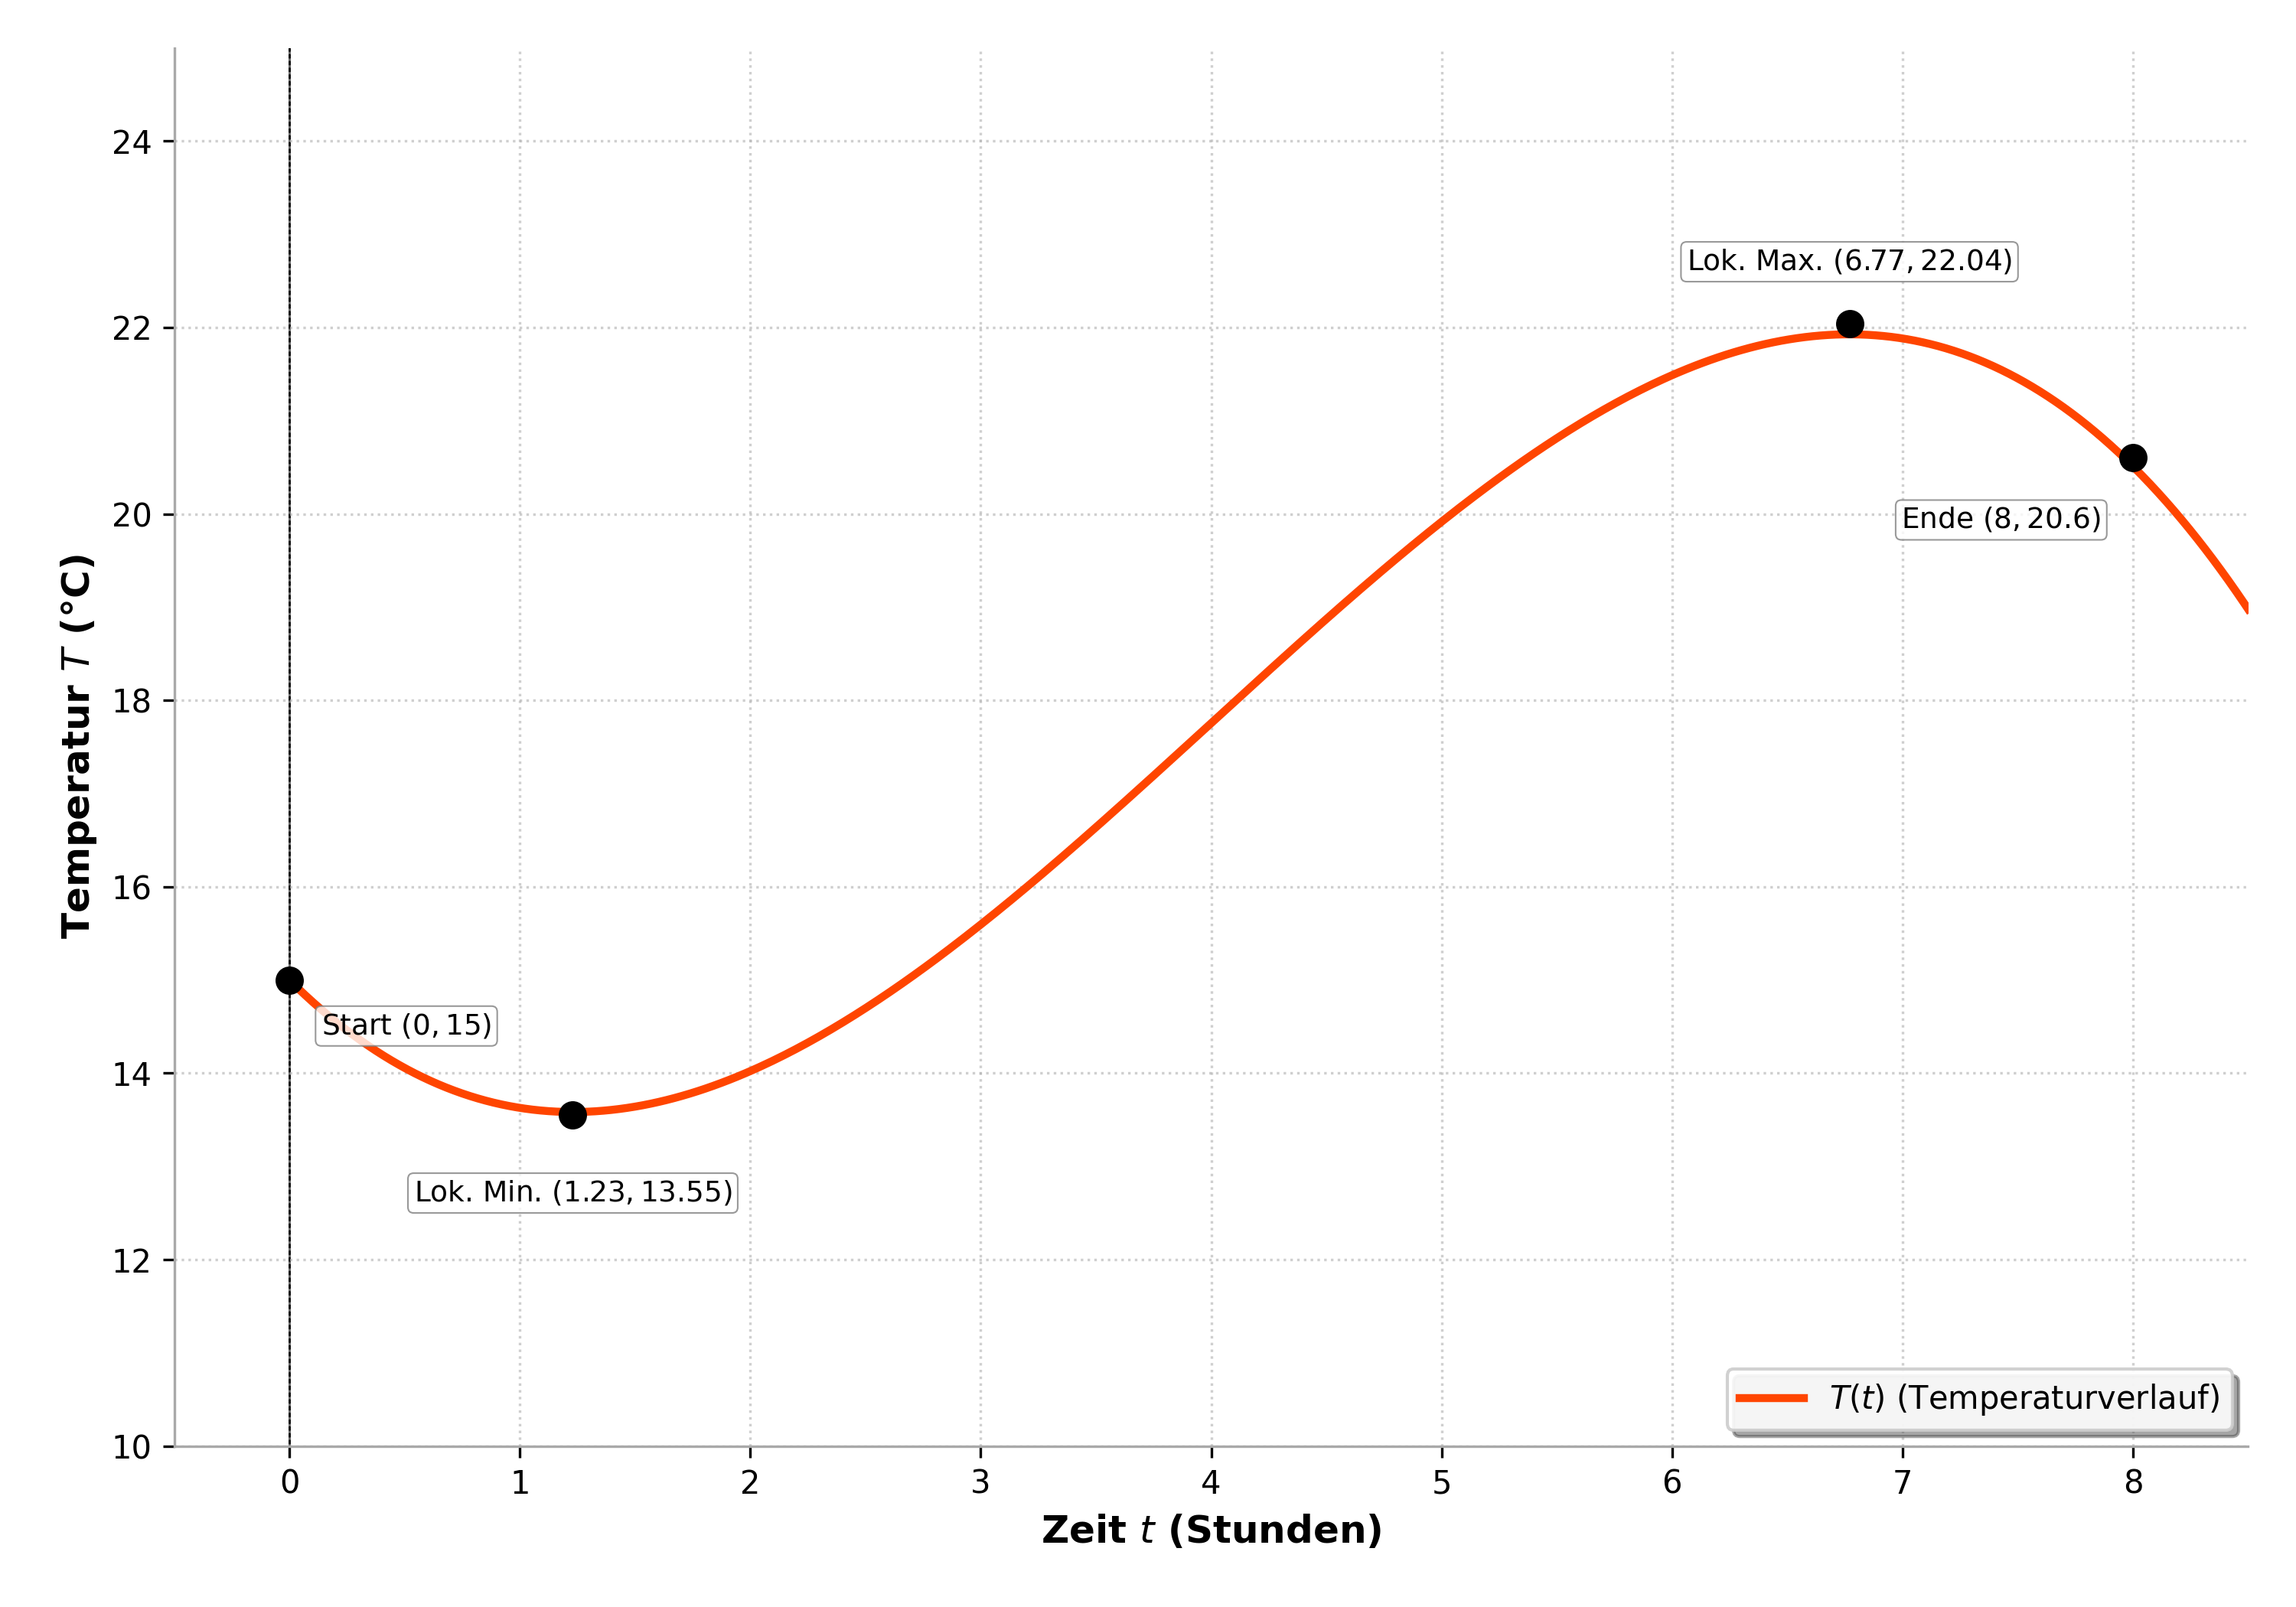
\includegraphics[width=0.8\textwidth]{grafiken/temperaturverlauf_graph.png}
        % --- Beschreibung der Grafik für T(t) ---
        % Die Grafik zeigt ein Koordinatensystem. t-Achse von 0 bis 8 (Stunden), T-Achse von ca. 10 bis 25 (Grad Celsius).
        % Der Graph startet bei (0|15). Fällt zu einem lokalen Minimum bei ca. (1.23|13.55).
        % Steigt zu einem lokalen Maximum bei ca. (6.77|22.04).
        % Fällt dann zum Endpunkt (8|20.6).
        % Die Kurve ist glatt und repräsentiert ein Polynom 3. Grades.
        \captionof{figure}{Skizze des Temperaturverlaufs $T(t)$.}
        \label{fig:temperaturverlauf}
        \end{center}
    \end{itemize}
\end{enumerate}

\end{loesungsumgebung}

\begin{aufgabenumgebung}{Extrempunkte finden – Vielfältige Herausforderungen}
Bestimme die lokalen Extrempunkte (Art und Koordinaten) der folgenden Funktionen. Verwende primär das \textbf{Vorzeichenwechselkriterium der ersten Ableitung ($f'(x)$)}. Du kannst deine Ergebnisse zusätzlich mit dem Kriterium der zweiten Ableitung ($f''(x)$) überprüfen, wo dies sinnvoll und einfach möglich ist.
\begin{enumerate}
    \item $f_1(x) = x^3 - 6x^2 + 9x + 1$


    \item $f_2(x) = \frac{1}{4}x^4 - x^3 - 2x^2 + 5$
        % \begin{tippumgebung}{Polynom 4. Grades}
        % Die erste Ableitung $f_2'(x)$ wird ein Polynom 3. Grades sein. Versuche, $x$ auszuklammern, um eine Nullstelle direkt zu finden. Die verbleibende quadratische Gleichung kannst du dann mit der p-q-Formel oder Mitternachtsformel lösen, um weitere Kandidaten für Extremstellen zu erhalten. Diese Funktion kann mehrere Extrempunkte haben.
        % \end{tippumgebung}

    \item $f_3(x) = x^4 - \frac{8}{3}x^3 + 2x^2$
        % \begin{tippumgebung}{Besonderer Fall bei $f_3''(x_E)=0$?}
        % Es kann vorkommen, dass für eine kritische Stelle $x_E$ (also $f_3'(x_E)=0$) auch die zweite Ableitung $f_3''(x_E)=0$ ist. In diesem Fall liefert das Kriterium mit der zweiten Ableitung keine Aussage über die Art des Extrempunkts. Dann musst du auf das Vorzeichenwechselkriterium der ersten Ableitung $f_3'(x)$ zurückgreifen, um zu entscheiden, ob ein Hochpunkt, Tiefpunkt oder vielleicht ein Sattelpunkt (kein Extremum) vorliegt.
        % \end{tippumgebung}

    \item \textbf{Schwer: Funktion mit Parameter $k$} \\
        Gegeben ist die Funktion $f_k(x) = x^3 - 3kx + 2$, wobei $k \in \mathbb{R}$ ein Parameter ist. Untersuche in Abhängigkeit von $k$:
        \begin{itemize}
            \item Für welche Werte von $k$ hat die Funktion $f_k(x)$ keine lokalen Extrempunkte?
            \item Für welche Werte von $k$ hat die Funktion $f_k(x)$ genau einen lokalen Extrempunkt? (Überlege, was das für die Ableitung bedeutet – kann ein Polynom 3. Grades nur einen Extrempunkt haben, wenn es nicht konstant ist?) Was liegt stattdessen an der kritischen Stelle vor, wenn es kein Extremum ist?
            \item Für welche Werte von $k$ hat die Funktion $f_k(x)$ genau zwei lokale Extrempunkte? Bestimme deren Art (Hoch-/Tiefpunkt) und ihre Lage (x-Koordinaten) in Abhängigkeit von $k$.
        \end{itemize}

    \item \textbf{Anwendung: Optimale Form}
        Ein oben offener quaderförmiger Behälter mit quadratischer Grundfläche soll ein Volumen von $V=32 \text{ cm}^3$ haben. Bestimme die Abmessungen (Seitenlänge der Grundfläche und Höhe), für die der Materialverbrauch (also die Oberfläche) minimal wird.
        \begin{enumerate}[label=(\alph*)]
            \item Sei $a$ die Seitenlänge der quadratischen Grundfläche und $h$ die Höhe des Quaders. Stelle die Formel für das Volumen $V$ und die Oberfläche $O$ (Grundfläche + 4 Seitenflächen) auf.
            \item Drücke $h$ mithilfe der Volumenformel durch $a$ aus (Nebenbedingung).
            \item Setze $h$ in die Oberflächenformel ein, um eine Zielfunktion $O(a)$ zu erhalten, die nur noch von $a$ abhängt.
            \item Bestimme die erste Ableitung $O'(a)$ und finde die kritischen Stellen.
            \item Überprüfe mit der zweiten Ableitung $O''(a)$, ob ein Minimum vorliegt. (Hier ist die zweite Ableitung oft der schnellste Weg zur Klassifizierung in Optimierungsaufgaben).
            \item Berechne die optimale Seitenlänge $a$ und die zugehörige Höhe $h$.
        \end{enumerate}
\end{enumerate}
\end{aufgabenumgebung}


\begin{loesungsumgebung}[loes:extrempunkte-vielfaeltig]{Extrempunkte finden – Vielfältige Herausforderungen}
Wir bestimmen die lokalen Extrempunkte der gegebenen Funktionen.

\begin{enumerate}[label=(\alph*)]
    \item \textbf{Funktion $f_1(x) = x^3 - 6x^2 + 9x + 1$}
    \begin{itemize}
        \item \textbf{Erste Ableitung:} $f_1'(x) = 3x^2 - 12x + 9$.
        \item \textbf{Notwendige Bedingung ($f_1'(x)=0$):}
        $3x^2 - 12x + 9 = 0 \quad | :3$
        $x^2 - 4x + 3 = 0$.
        Mit p-q-Formel oder Vieta: $(x-1)(x-3)=0$.
        Kandidaten für Extremstellen: $x_E_1 = 1$, $x_E_2 = 3$.
        \item \textbf{Vorzeichenwechselkriterium von $f_1'(x)$:}
        $f_1'(x) = 3(x-1)(x-3)$ ist eine nach oben geöffnete Parabel.
        \begin{itemize}
            \item Für $x < 1$ (z.B. $x=0$): $f_1'(0) = 9 > 0$ ($f_1$ steigt).
            \item Für $1 < x < 3$ (z.B. $x=2$): $f_1'(2) = 3(4)-12(2)+9 = 12-24+9 = -3 < 0$ ($f_1$ fällt).
            \item Für $x > 3$ (z.B. $x=4$): $f_1'(4) = 3(16)-12(4)+9 = 48-48+9 = 9 > 0$ ($f_1$ steigt).
        \end{itemize}
        \item \textbf{Art und Koordinaten der Extrempunkte:}
        \begin{itemize}
            \item Bei $x_E_1 = 1$: Vorzeichenwechsel von $f_1'(x)$ von $+$ nach $- \Rightarrow$ \textbf{Lokaler Hochpunkt}.
            $y_E_1 = f_1(1) = 1^3 - 6(1)^2 + 9(1) + 1 = 1-6+9+1 = 5$.
            $\rightarrow HP(1|5)$.
            \item Bei $x_E_2 = 3$: Vorzeichenwechsel von $f_1'(x)$ von $-$ nach $+ \Rightarrow$ \textbf{Lokaler Tiefpunkt}.
            $y_E_2 = f_1(3) = 3^3 - 6(3)^2 + 9(3) + 1 = 27 - 54 + 27 + 1 = 1$.
            $\rightarrow TP(3|1)$.
        \end{itemize}
        \item \textbf{Überprüfung mit $f_1''(x)$:}
        $f_1''(x) = 6x - 12$.
        $f_1''(1) = 6(1)-12 = -6 < 0 \Rightarrow$ Hochpunkt.
        $f_1''(3) = 6(3)-12 = 18-12 = 6 > 0 \Rightarrow$ Tiefpunkt. (Bestätigt)
    \end{itemize}

    \item \textbf{Funktion $f_2(x) = \frac{1}{4}x^4 - x^3 - 2x^2 + 5$}
    \begin{itemize}
        \item \textbf{Erste Ableitung:} $f_2'(x) = x^3 - 3x^2 - 4x$.
        \item \textbf{Notwendige Bedingung ($f_2'(x)=0$):}
        $x^3 - 3x^2 - 4x = 0 \Rightarrow x(x^2 - 3x - 4) = 0$.
        $x_E_1 = 0$.
        Für $x^2 - 3x - 4 = 0$: $(x-4)(x+1)=0 \Rightarrow x_E_2 = 4$, $x_E_3 = -1$.
        Kandidaten: $x=-1, 0, 4$.
        \item \textbf{Vorzeichenwechselkriterium von $f_2'(x) = x(x+1)(x-4)$:}
        \begin{itemize}
            \item Intervall $(-\infty, -1)$ (z.B. $x=-2$): $f_2'(-2) = (-2)(-1)(-6) = -12 < 0$.
            \item Intervall $(-1, 0)$ (z.B. $x=-0.5$): $f_2'(-0.5) = (-0.5)(0.5)(-4.5) = 1.125 > 0$.
            \item Intervall $(0, 4)$ (z.B. $x=1$): $f_2'(1) = (1)(2)(-3) = -6 < 0$.
            \item Intervall $(4, \infty)$ (z.B. $x=5$): $f_2'(5) = (5)(6)(1) = 30 > 0$.
        \end{itemize}
        \item \textbf{Art und Koordinaten der Extrempunkte:}
        \begin{itemize}
            \item Bei $x_E_3 = -1$: VZW von $-$ nach $+ \Rightarrow$ \textbf{Lokaler Tiefpunkt}.
            $f_2(-1) = \frac{1}{4}(1) - (-1) - 2(1) + 5 = \frac{1}{4} + 1 - 2 + 5 = 4.25 = \frac{17}{4}$.
            $\rightarrow TP(-1|4.25)$.
            \item Bei $x_E_1 = 0$: VZW von $+$ nach $- \Rightarrow$ \textbf{Lokaler Hochpunkt}.
            $f_2(0) = 5$.
            $\rightarrow HP(0|5)$.
            \item Bei $x_E_2 = 4$: VZW von $-$ nach $+ \Rightarrow$ \textbf{Lokaler Tiefpunkt}.
            $f_2(4) = \frac{1}{4}(256) - 64 - 2(16) + 5 = 64 - 64 - 32 + 5 = -27$.
            $\rightarrow TP(4|-27)$.
        \end{itemize}
        \item \textbf{Überprüfung mit $f_2''(x)$:}
        $f_2''(x) = 3x^2 - 6x - 4$.
        $f_2''(-1) = 3(1) - 6(-1) - 4 = 3+6-4 = 5 > 0 \Rightarrow$ Tiefpunkt.
        $f_2''(0) = -4 < 0 \Rightarrow$ Hochpunkt.
        $f_2''(4) = 3(16) - 6(4) - 4 = 48 - 24 - 4 = 20 > 0 \Rightarrow$ Tiefpunkt. (Bestätigt)
    \end{itemize}

    \item \textbf{Funktion $f_3(x) = x^4 - \frac{8}{3}x^3 + 2x^2$}
    \begin{itemize}
        \item \textbf{Erste Ableitung:} $f_3'(x) = 4x^3 - 8x^2 + 4x$.
        \item \textbf{Notwendige Bedingung ($f_3'(x)=0$):}
        $4x^3 - 8x^2 + 4x = 0 \Rightarrow 4x(x^2 - 2x + 1) = 0 \Rightarrow 4x(x-1)^2 = 0$.
        Kandidaten: $x_E_1 = 0$, $x_E_2 = 1$.
        \item \textbf{Vorzeichenwechselkriterium von $f_3'(x) = 4x(x-1)^2$:}
        Der Faktor $(x-1)^2$ ist immer $\ge 0$. Das Vorzeichen von $f_3'(x)$ (außer bei $x=1$) wird also durch $4x$ bestimmt.
        \begin{itemize}
            \item Für $x < 0$ (z.B. $x=-1$): $f_3'(-1) = 4(-1)(-1-1)^2 = -4(4) = -16 < 0$.
            \item Für $0 < x < 1$ (z.B. $x=0.5$): $f_3'(0.5) = 4(0.5)(0.5-1)^2 = 2(-0.5)^2 = 2(0.25) = 0.5 > 0$.
            \item Für $x > 1$ (z.B. $x=2$): $f_3'(2) = 4(2)(2-1)^2 = 8(1)^2 = 8 > 0$.
        \end{itemize}
        \item \textbf{Art und Koordinaten der Extrempunkte:}
        \begin{itemize}
            \item Bei $x_E_1 = 0$: VZW von $-$ nach $+ \Rightarrow$ \textbf{Lokaler Tiefpunkt}.
            $f_3(0) = 0$.
            $\rightarrow TP(0|0)$.
            \item Bei $x_E_2 = 1$: Kein VZW (von $+$ nach $+$) $\Rightarrow$ \textbf{Sattelpunkt (Terrassenpunkt)}, kein Extremum.
            $f_3(1) = 1 - \frac{8}{3} + 2 = 3 - \frac{8}{3} = \frac{9-8}{3} = \frac{1}{3}$.
            $\rightarrow SP(1|\frac{1}{3})$.
        \end{itemize}
        \item \textbf{Überprüfung mit $f_3''(x)$:}
        $f_3''(x) = 12x^2 - 16x + 4$.
        $f_3''(0) = 4 > 0 \Rightarrow$ Tiefpunkt.
        $f_3''(1) = 12(1)^2 - 16(1) + 4 = 12 - 16 + 4 = 0$. Das Kriterium mit $f_3''(x)$ liefert hier keine Aussage für $x=1$, wie im Tipp erwähnt. Das Vorzeichenwechselkriterium von $f_3'(x)$ hat bereits gezeigt, dass es sich um einen Sattelpunkt handelt.
    \end{itemize}

    \item \textbf{Schwer: Funktion mit Parameter $k$: $f_k(x) = x^3 - 3kx + 2$}
    \begin{itemize}
        \item \textbf{Erste Ableitung:} $f_k'(x) = 3x^2 - 3k$.
        \item \textbf{Notwendige Bedingung ($f_k'(x)=0$):}
        $3x^2 - 3k = 0 \Rightarrow 3x^2 = 3k \Rightarrow x^2 = k$.
        \item \textbf{Fallunterscheidung basierend auf $k$ für $x^2=k$:}
        \begin{itemize}
            \item \textbf{Fall 1: $k < 0$} \\
            Die Gleichung $x^2=k$ hat keine reellen Lösungen, da $x^2 \ge 0$.
            $f_k'(x) = 3x^2 - 3k = 3x^2 + 3|k|$. Da $3x^2 \ge 0$ und $3|k| > 0$ (wenn $k \neq 0$), ist $f_k'(x) > 0$ für alle $x$.
            Die Funktion $f_k(x)$ ist streng monoton steigend und hat \textbf{keine lokalen Extrempunkte}.
            \item \textbf{Fall 2: $k = 0$} \\
            Die Gleichung $x^2=0$ hat die einzige Lösung $x_E=0$.
            $f_0'(x) = 3x^2$.
            Für $x<0$ ist $f_0'(x) > 0$. Für $x>0$ ist $f_0'(x) > 0$.
            Es gibt keinen Vorzeichenwechsel bei $x=0$. $f_0(x)$ hat bei $x=0$ einen \textbf{Sattelpunkt}, aber \textbf{keinen lokalen Extrempunkt}.
            \item \textbf{Fall 3: $k > 0$} \\
            Die Gleichung $x^2=k$ hat zwei verschiedene reelle Lösungen: $x_E_1 = -\sqrt{k}$ und $x_E_2 = \sqrt{k}$.
            $f_k'(x) = 3x^2 - 3k = 3(x^2-k)$. Dies ist eine nach oben geöffnete Parabel mit Nullstellen bei $\pm\sqrt{k}$.
            \begin{itemize}
                \item Für $x < -\sqrt{k}$: $f_k'(x) > 0$.
                \item Für $-\sqrt{k} < x < \sqrt{k}$: $f_k'(x) < 0$.
                \item Für $x > \sqrt{k}$: $f_k'(x) > 0$.
            \end{itemize}
            Bei $x_E_1 = -\sqrt{k}$: VZW von $+$ nach $- \Rightarrow$ \textbf{Lokaler Hochpunkt}.
            Bei $x_E_2 = \sqrt{k}$: VZW von $-$ nach $+ \Rightarrow$ \textbf{Lokaler Tiefpunkt}.
            Die Funktion $f_k(x)$ hat \textbf{genau zwei lokale Extrempunkte}.
        \end{itemize}
        \item \textbf{Antworten auf die Fragen:}
        \begin{itemize}
            \item Keine lokalen Extrempunkte: Für $k \le 0$.
            \item Genau einen lokalen Extrempunkt: Ein Polynom 3. Grades hat entweder zwei lokale Extrema oder keinen (im Fall eines Sattelpunkts). Es gibt also keinen Fall mit genau einem lokalen Extremum (Hoch- oder Tiefpunkt). Für $k=0$ gibt es einen Sattelpunkt, was kein Extremum ist.
            \item Genau zwei lokale Extrempunkte: Für $k > 0$.
            Lage: $x_{HP} = -\sqrt{k}$ (Hochpunkt), $x_{TP} = \sqrt{k}$ (Tiefpunkt).
        \end{itemize}
    \end{itemize}

    \item \textbf{Anwendung: Optimale Form eines Behälters}
    Gegeben: Oben offener Quader, quadratische Grundfläche $a \cdot a$, Höhe $h$, Volumen $V=32 \text{ cm}^3$. Gesucht: Minimale Oberfläche $O$.
    \begin{enumerate}[label=(\roman*)]
        \item \textbf{Formeln für Volumen $V$ und Oberfläche $O$:}
        $V = a^2 h$
        $O = \text{Grundfläche} + \text{Mantelfläche} = a^2 + 4ah$
        \item \textbf{$h$ durch $a$ ausdrücken (Nebenbedingung):}
        Aus $V=32$: $a^2h = 32 \Rightarrow h = \frac{32}{a^2}$ (gültig für $a>0$).
        \item \textbf{Zielfunktion $O(a)$:}
        $h$ in $O$ einsetzen:
        $O(a) = a^2 + 4a \left(\frac{32}{a^2}\right) = a^2 + \frac{128}{a} = a^2 + 128a^{-1}$.
        \item \textbf{Erste Ableitung $O'(a)$ und kritische Stellen:}
        $O'(a) = \frac{d}{da}(a^2 + 128a^{-1}) = 2a - 128a^{-2} = 2a - \frac{128}{a^2}$.
        Setze $O'(a)=0$ für kritische Stellen:
        $2a - \frac{128}{a^2} = 0 \quad | \cdot a^2 \quad (a \neq 0)$
        $2a^3 - 128 = 0$
        $$
        \begin{array}{r c l c l}
        \umformung{2a^3 - 128}{0}{+}{128}
        \umformung{2a^3}{128}{\div}{2}
        \umformung{a^3}{64}{\text{dritte Wurzel ziehen}}{}
        \umformungend{a}{4}
        \end{array}
        $$
        Die einzige positive kritische Stelle ist $a=4\,$cm.
        \item \textbf{Überprüfung mit der zweiten Ableitung $O''(a)$:}
        $O''(a) = \frac{d}{da}(2a - 128a^{-2}) = 2 - 128(-2)a^{-3} = 2 + 256a^{-3} = 2 + \frac{256}{a^3}$.
        Für $a=4$: $O''(4) = 2 + \frac{256}{4^3} = 2 + \frac{256}{64} = 2 + 4 = 6$.
        Da $O''(4) = 6 > 0$, liegt bei $a=4$ ein lokales Minimum für die Oberfläche vor.
        \item \textbf{Optimale Seitenlänge $a$ und Höhe $h$:}
        Die optimale Seitenlänge der Grundfläche ist $a = 4\,$cm.
        Die zugehörige Höhe ist $h = \frac{32}{a^2} = \frac{32}{4^2} = \frac{32}{16} = 2\,$cm.
        Die Abmessungen für den minimalen Materialverbrauch sind $4\,$cm $\cdot$ $4\,$cm für die Grundfläche und $2\,$cm für die Höhe.
    \end{enumerate}
\end{enumerate}

\end{loesungsumgebung}

\begin{aufgabenumgebung}{Höhere Ableitungen berechnen}
Bestimme die erste, zweite und dritte Ableitung der folgenden Funktionen:
\begin{enumerate}
    \item $f(x) = 2x^3 - 9x^2 + 12x - 5$
    \item $g(x) = -0.1x^5 + x^3 - 7$
    \item $h(t) = 2t^2 - \frac{1}{t}$ (Tipp: $\frac{1}{t} = t^{-1}$)
\end{enumerate}
\end{aufgabenumgebung}

\begin{loesungsumgebung}[loes:hoehere-ableitungen]{Höhere Ableitungen berechnen}
Wir bestimmen die erste ($f'(x)$), zweite ($f''(x)$) und dritte ($f'''(x)$) Ableitung der gegebenen Funktionen.

\begin{enumerate}[label=(\alph*)]
    \item \textbf{Funktion $f(x) = 2x^3 - 9x^2 + 12x - 5$}
    \begin{itemize}
        \item \textbf{Erste Ableitung $f'(x)$:}
        $$ f'(x) = \frac{d}{dx}(2x^3 - 9x^2 + 12x - 5) $$
        $$ f'(x) = 2 \cdot 3x^{3-1} - 9 \cdot 2x^{2-1} + 12 \cdot 1x^{1-1} - 0 $$
        $$ f'(x) = 6x^2 - 18x + 12 $$
        \item \textbf{Zweite Ableitung $f''(x)$:}
        $$ f''(x) = \frac{d}{dx}(6x^2 - 18x + 12) $$
        $$ f''(x) = 6 \cdot 2x^{2-1} - 18 \cdot 1x^{1-1} + 0 $$
        $$ f''(x) = 12x - 18 $$
        \item \textbf{Dritte Ableitung $f'''(x)$:}
        $$ f'''(x) = \frac{d}{dx}(12x - 18) $$
        $$ f'''(x) = 12 \cdot 1x^{1-1} - 0 $$
        $$ f'''(x) = 12 $$
    \end{itemize}

    \item \textbf{Funktion $g(x) = -0.1x^5 + x^3 - 7$}
    \begin{itemize}
        \item \textbf{Erste Ableitung $g'(x)$:}
        $$ g'(x) = \frac{d}{dx}(-0.1x^5 + x^3 - 7) $$
        $$ g'(x) = -0.1 \cdot 5x^{5-1} + 3x^{3-1} - 0 $$
        $$ g'(x) = -0.5x^4 + 3x^2 $$
        \item \textbf{Zweite Ableitung $g''(x)$:}
        $$ g''(x) = \frac{d}{dx}(-0.5x^4 + 3x^2) $$
        $$ g''(x) = -0.5 \cdot 4x^{4-1} + 3 \cdot 2x^{2-1} $$
        $$ g''(x) = -2x^3 + 6x $$
        \item \textbf{Dritte Ableitung $g'''(x)$:}
        $$ g'''(x) = \frac{d}{dx}(-2x^3 + 6x) $$
        $$ g'''(x) = -2 \cdot 3x^{3-1} + 6 \cdot 1x^{1-1} $$
        $$ g'''(x) = -6x^2 + 6 $$
    \end{itemize}

    \item \textbf{Funktion $h(t) = 2t^2 - \frac{1}{t}$} \\
    Zuerst schreiben wir die Funktion mit Potenzschreibweise um: $h(t) = 2t^2 - t^{-1}$.
    \begin{itemize}
        \item \textbf{Erste Ableitung $h'(t)$:}
        $$ h'(t) = \frac{d}{dt}(2t^2 - t^{-1}) $$
        $$ h'(t) = 2 \cdot 2t^{2-1} - (-1)t^{-1-1} $$
        $$ h'(t) = 4t + t^{-2} = 4t + \frac{1}{t^2} $$
        \item \textbf{Zweite Ableitung $h''(t)$:}
        $$ h''(t) = \frac{d}{dt}(4t + t^{-2}) $$
        $$ h''(t) = 4 \cdot 1t^{1-1} + (-2)t^{-2-1} $$
        $$ h''(t) = 4 - 2t^{-3} = 4 - \frac{2}{t^3} $$
        \item \textbf{Dritte Ableitung $h'''(t)$:}
        $$ h'''(t) = \frac{d}{dt}(4 - 2t^{-3}) $$
        $$ h'''(t) = 0 - 2(-3)t^{-3-1} $$
        $$ h'''(t) = 6t^{-4} = \frac{6}{t^4} $$
    \end{itemize}
\end{enumerate}

\end{loesungsumgebung}

\begin{aufgabenumgebung}{Krümmung und Wendepunkte – Vielfältige Untersuchungen}
Untersuche die folgenden Funktionen auf ihr Krümmungsverhalten (Intervalle für Links- und Rechtskrümmung) und bestimme gegebenenfalls die Koordinaten der Wendepunkte. Nutze dazu die zweite und, falls nötig, die dritte Ableitung.
\begin{enumerate}
    \item $f_1(x) = \frac{1}{12}x^4 - \frac{1}{2}x^3 + x^2 + 1$
    \item $f_2(x) = x^5 - 5x^4 + 3x - 2$


    \item \textbf{Anwendung: Infektionsgeschehen} \\
        Die Funktion $N(t) = -t^3 + 12t^2 + 20t$ beschreibt die Anzahl der neu infizierten Personen pro Tag während einer Grippewelle ($t$ in Tagen, $t \ge 0$).
        \begin{itemize}
            \item Bestimme die Funktion $N'(t)$, welche die Änderungsrate der Neuinfektionen (also die 'Geschwindigkeit' der Ausbreitung) beschreibt.
            \item Bestimme die Funktion $N''(t)$, welche die Änderungsrate der Wachstumsrate der Neuinfektionen beschreibt.
            \item Zu welchem Zeitpunkt $t_W$ ist die Zunahme der täglichen Neuinfektionen am größten? (Das bedeutet, $N'(t)$ hat ein Maximum, also suche einen Wendepunkt von $N(t)$, an dem die Krümmung von links nach rechts wechselt, d.h. $N''(t_W)=0$ und $N'''(t_W)<0$).
            \item Interpretiere die Bedeutung dieses Zeitpunktes $t_W$ für den Verlauf der Grippewelle. Was passiert mit der Zunahme der Neuinfektionen nach diesem Zeitpunkt?
        \end{itemize}

    \item \textbf{Schwer: Funktion mit Parameter $a$} \\
        Gegeben ist die Funktionenschar $f_a(x) = x^4 + ax^3$ mit $a \in \mathbb{R}, a \neq 0$.
        \begin{itemize}
            \item Bestimme die zweite Ableitung $f_a''(x)$.
            \item Zeige, dass $x_1=0$ eine potentielle Wendestelle ist. Untersuche mit der dritten Ableitung $f_a'''(x)$, ob für $x_1=0$ tatsächlich ein Wendepunkt vorliegt.
            \item Bestimme die andere potentielle Wendestelle $x_2$ in Abhängigkeit von $a$.
            \item Für welche Werte von $a$ existiert dieser zweite Wendepunkt $x_2$? (Beachte, dass $x_2 \neq x_1$ sein sollte für einen \textit{anderen} Wendepunkt).
            \item Untersuche das Krümmungsverhalten für $a=2$ und $a=-2$ und skizziere grob die Verläufe (ohne vollständige Kurvendiskussion, Fokus auf Krümmung und Wendepunkte).
        \end{itemize}
\end{enumerate}
\end{aufgabenumgebung}


\begin{loesungsumgebung}[loes:kruemmung-wendepunkte-vielfalt]{Krümmung und Wendepunkte – Vielfältige Untersuchungen}
Wir untersuchen die gegebenen Funktionen auf ihr Krümmungsverhalten und bestimmen die Koordinaten eventueller Wendepunkte.

\begin{enumerate}[label=(\alph*)]
    \item \textbf{Funktion $f_1(x) = \frac{1}{12}x^4 - \frac{1}{2}x^3 + x^2 + 1$}
    \begin{itemize}
        \item \textbf{Erste Ableitung:} $f_1'(x) = \frac{4}{12}x^3 - \frac{3}{2}x^2 + 2x = \frac{1}{3}x^3 - \frac{3}{2}x^2 + 2x$.
        \item \textbf{Zweite Ableitung:} $f_1''(x) = 3 \cdot \frac{1}{3}x^2 - 2 \cdot \frac{3}{2}x + 2 = x^2 - 3x + 2$.
        \item \textbf{Nullstellen der zweiten Ableitung ($f_1''(x)=0$):}
        $x^2 - 3x + 2 = 0$. Mit dem Satz von Vieta (oder p-q-Formel): $(x-1)(x-2)=0$.
        Potentielle Wendestellen sind $x_{W1} = 1$ und $x_{W2} = 2$.
        \item \textbf{Dritte Ableitung:} $f_1'''(x) = 2x - 3$.
        \item \textbf{Überprüfung der potentiellen Wendestellen:}
        \begin{itemize}
            \item Für $x_{W1} = 1$: $f_1'''(1) = 2(1) - 3 = -1 \neq 0$. Also liegt bei $x=1$ ein Wendepunkt vor.
            \item Für $x_{W2} = 2$: $f_1'''(2) = 2(2) - 3 = 1 \neq 0$. Also liegt bei $x=2$ ein Wendepunkt vor.
        \end{itemize}
        \item \textbf{Krümmungsverhalten ($f_1''(x) = x^2 - 3x + 2$ ist eine nach oben geöffnete Parabel):}
        \begin{itemize}
            \item Für $x < 1$: $f_1''(x) > 0 \Rightarrow$ Linkskrümmung (konvex).
            \item Für $1 < x < 2$: $f_1''(x) < 0 \Rightarrow$ Rechtskrümmung (konkav).
            \item Für $x > 2$: $f_1''(x) > 0 \Rightarrow$ Linkskrümmung (konvex).
        \end{itemize}
        \item \textbf{Koordinaten der Wendepunkte:}
        \begin{itemize}
            \item $y_{W1} = f_1(1) = \frac{1}{12}(1)^4 - \frac{1}{2}(1)^3 + (1)^2 + 1 = \frac{1}{12} - \frac{1}{2} + 1 + 1 = \frac{1-6+12+12}{12} = \frac{19}{12}$.
            $\rightarrow WP_1(1|\frac{19}{12})$.
            \item $y_{W2} = f_1(2) = \frac{1}{12}(2)^4 - \frac{1}{2}(2)^3 + (2)^2 + 1 = \frac{16}{12} - \frac{8}{2} + 4 + 1 = \frac{4}{3} - 4 + 4 + 1 = \frac{4}{3} + 1 = \frac{7}{3}$.
            $\rightarrow WP_2(2|\frac{7}{3})$.
        \end{itemize}
    \end{itemize}

    \item \textbf{Funktion $f_2(x) = x^5 - 5x^4 + 3x - 2$}
    \begin{itemize}
        \item \textbf{Erste Ableitung:} $f_2'(x) = 5x^4 - 20x^3 + 3$.
        \item \textbf{Zweite Ableitung:} $f_2''(x) = 20x^3 - 60x^2$.
        \item \textbf{Nullstellen der zweiten Ableitung ($f_2''(x)=0$):}
        $20x^3 - 60x^2 = 0 \Rightarrow 20x^2(x-3) = 0$.
        Potentielle Wendestellen sind $x_{W1} = 0$ und $x_{W2} = 3$.
        \item \textbf{Dritte Ableitung:} $f_2'''(x) = 60x^2 - 120x = 60x(x-2)$.
        \item \textbf{Überprüfung der potentiellen Wendestellen:}
        \begin{itemize}
            \item Für $x_{W1} = 0$: $f_2'''(0) = 60(0)(0-2) = 0$. Hier liefert $f_2'''(x)$ keine Aussage. Wir müssen das Vorzeichen von $f_2''(x)$ untersuchen.
            \item Für $x_{W2} = 3$: $f_2'''(3) = 60(3)(3-2) = 180 \neq 0$. Also liegt bei $x=3$ ein Wendepunkt vor.
        \end{itemize}
        \item \textbf{Krümmungsverhalten ($f_2''(x) = 20x^2(x-3)$):}
        Der Faktor $20x^2$ ist für $x \neq 0$ positiv. Das Vorzeichen von $f_2''(x)$ wird also (für $x \neq 0$) durch $(x-3)$ bestimmt.
        \begin{itemize}
            \item Für $x < 0$: $x-3 < 0 \Rightarrow f_2''(x) < 0 \Rightarrow$ Rechtskrümmung.
            \item Für $0 < x < 3$: $x-3 < 0 \Rightarrow f_2''(x) < 0 \Rightarrow$ Rechtskrümmung.
            \item Für $x > 3$: $x-3 > 0 \Rightarrow f_2''(x) > 0 \Rightarrow$ Linkskrümmung.
        \end{itemize}
        An der Stelle $x=0$ wechselt $f_2''(x)$ das Vorzeichen nicht (es ist $f_2''(x) \le 0$ in der Umgebung von $x=0$). Daher ist bei $x=0$ \textbf{kein Wendepunkt}.
        \item \textbf{Koordinaten des Wendepunkts:}
        \begin{itemize}
            \item $y_{W2} = f_2(3) = (3)^5 - 5(3)^4 + 3(3) - 2 = 243 - 5(81) + 9 - 2 = 243 - 405 + 7 = -155$.
            $\rightarrow WP(3|-155)$.
        \end{itemize}
    \end{itemize}

    \item \textbf{Anwendung: Infektionsgeschehen $N(t) = -t^3 + 12t^2 + 20t$ ($t \ge 0$)}
    \begin{itemize}
        \item \textbf{$N'(t)$ (Änderungsrate der Neuinfektionen):}
        $N'(t) = -3t^2 + 24t + 20$.
        \item \textbf{$N''(t)$ (Änderungsrate der Wachstumsrate):}
        $N''(t) = -6t + 24$.
        \item \textbf{Zeitpunkt $t_W$ der größten Zunahme der Neuinfektionen:}
        Dies ist der Zeitpunkt, an dem $N'(t)$ ein Maximum hat, also $N''(t_W)=0$ und $N'''(t_W)<0$.
        $N''(t_W)=0 \Rightarrow -6t_W + 24 = 0 \Rightarrow 6t_W = 24 \Rightarrow t_W = 4$.
        Die dritte Ableitung ist $N'''(t) = -6$.
        Da $N'''(4) = -6 < 0$, hat $N'(t)$ bei $t_W=4$ ein Maximum. Der Punkt $t_W=4$ ist ein Wendepunkt der Funktion $N(t)$, an dem die Krümmung von einer Linkskrümmung ($N''(t)>0$ für $t<4$) zu einer Rechtskrümmung ($N''(t)<0$ für $t>4$) wechselt.
        Der Zeitpunkt, an dem die Zunahme der täglichen Neuinfektionen am größten ist, ist $t_W = 4$ Tage.
        \item \textbf{Interpretation von $t_W=4$:}
        Am 4. Tag nach Beobachtungsbeginn ist der Anstieg der Zahl der täglichen Neuinfektionen am stärksten. Bis zu diesem Zeitpunkt beschleunigt sich die Ausbreitung der Grippewelle (die Zahl der Neuinfektionen pro Tag steigt immer schneller). Nach dem 4. Tag nehmen die täglichen Neuinfektionen zwar möglicherweise immer noch zu (solange $N'(t)>0$), aber die Geschwindigkeit dieser Zunahme verlangsamt sich. Der Wendepunkt markiert den Übergang von exponentiell anmutendem Wachstum zu einem gebremsten Wachstum der Neuinfektionszahlen pro Tag.
    \end{itemize}

    \item \textbf{Schwer: Funktion mit Parameter $a$: $f_a(x) = x^4 + ax^3$ ($a \in \mathbb{R}, a \neq 0$)}
    \begin{itemize}
        \item \textbf{Zweite Ableitung $f_a''(x)$:}
        $f_a'(x) = 4x^3 + 3ax^2$.
        $f_a''(x) = 12x^2 + 6ax = 6x(2x+a)$.
        \item \textbf{Untersuchung von $x_1=0$ als potentielle Wendestelle:}
        $f_a''(0) = 6(0)(2(0)+a) = 0$. Also ist $x_1=0$ eine potentielle Wendestelle.
        Dritte Ableitung: $f_a'''(x) = 24x + 6a$.
        $f_a'''(0) = 24(0) + 6a = 6a$.
        Da $a \neq 0$ (laut Aufgabenstellung), ist $f_a'''(0) = 6a \neq 0$.
        Somit liegt bei $x_1=0$ tatsächlich ein Wendepunkt vor.
        \item \textbf{Andere potentielle Wendestelle $x_2$:}
        Aus $f_a''(x) = 6x(2x+a)=0$ folgt neben $x_1=0$ auch $2x+a=0$.
        $2x = -a \Rightarrow x_2 = -\frac{a}{2}$.
        \item \textbf{Existenz des zweiten Wendepunkts $x_2$:}
        Der Wendepunkt $x_2 = -\frac{a}{2}$ existiert für alle $a \in \mathbb{R}$.
        Damit es ein \textit{anderer} Wendepunkt als $x_1=0$ ist, muss $x_2 \neq 0$, also $-\frac{a}{2} \neq 0$. Dies ist erfüllt, da $a \neq 0$ vorgegeben ist.
        Also gibt es für alle $a \neq 0$ zwei verschiedene Wendepunkte bei $x=0$ und $x=-a/2$. (Überprüfung für $x_2$: $f_a'''(-a/2) = 24(-a/2) + 6a = -12a + 6a = -6a$. Da $a \neq 0$, ist $f_a'''(-a/2) \neq 0$).
        \item \textbf{Krümmungsverhalten und Skizzen für $a=2$ und $a=-2$:}
        \begin{itemize}
            \item \textbf{Fall $a=2$:} $f_2(x) = x^4 + 2x^3$.
            $f_2''(x) = 12x^2 + 12x = 12x(x+1)$.
            Wendestellen bei $x_{W_1}=0$ und $x_{W_2}=-1$.
            $f_2''(x)$ ist eine nach oben geöffnete Parabel.
            Krümmungsverhalten:
            \begin{itemize}
                \item $(-\infty, -1)$: $f_2''(x) > 0 \Rightarrow$ Linkskrümmung.
                \item $(-1, 0)$: $f_2''(x) < 0 \Rightarrow$ Rechtskrümmung.
                \item $(0, \infty)$: $f_2''(x) > 0 \Rightarrow$ Linkskrümmung.
            \end{itemize}
            \begin{center}
            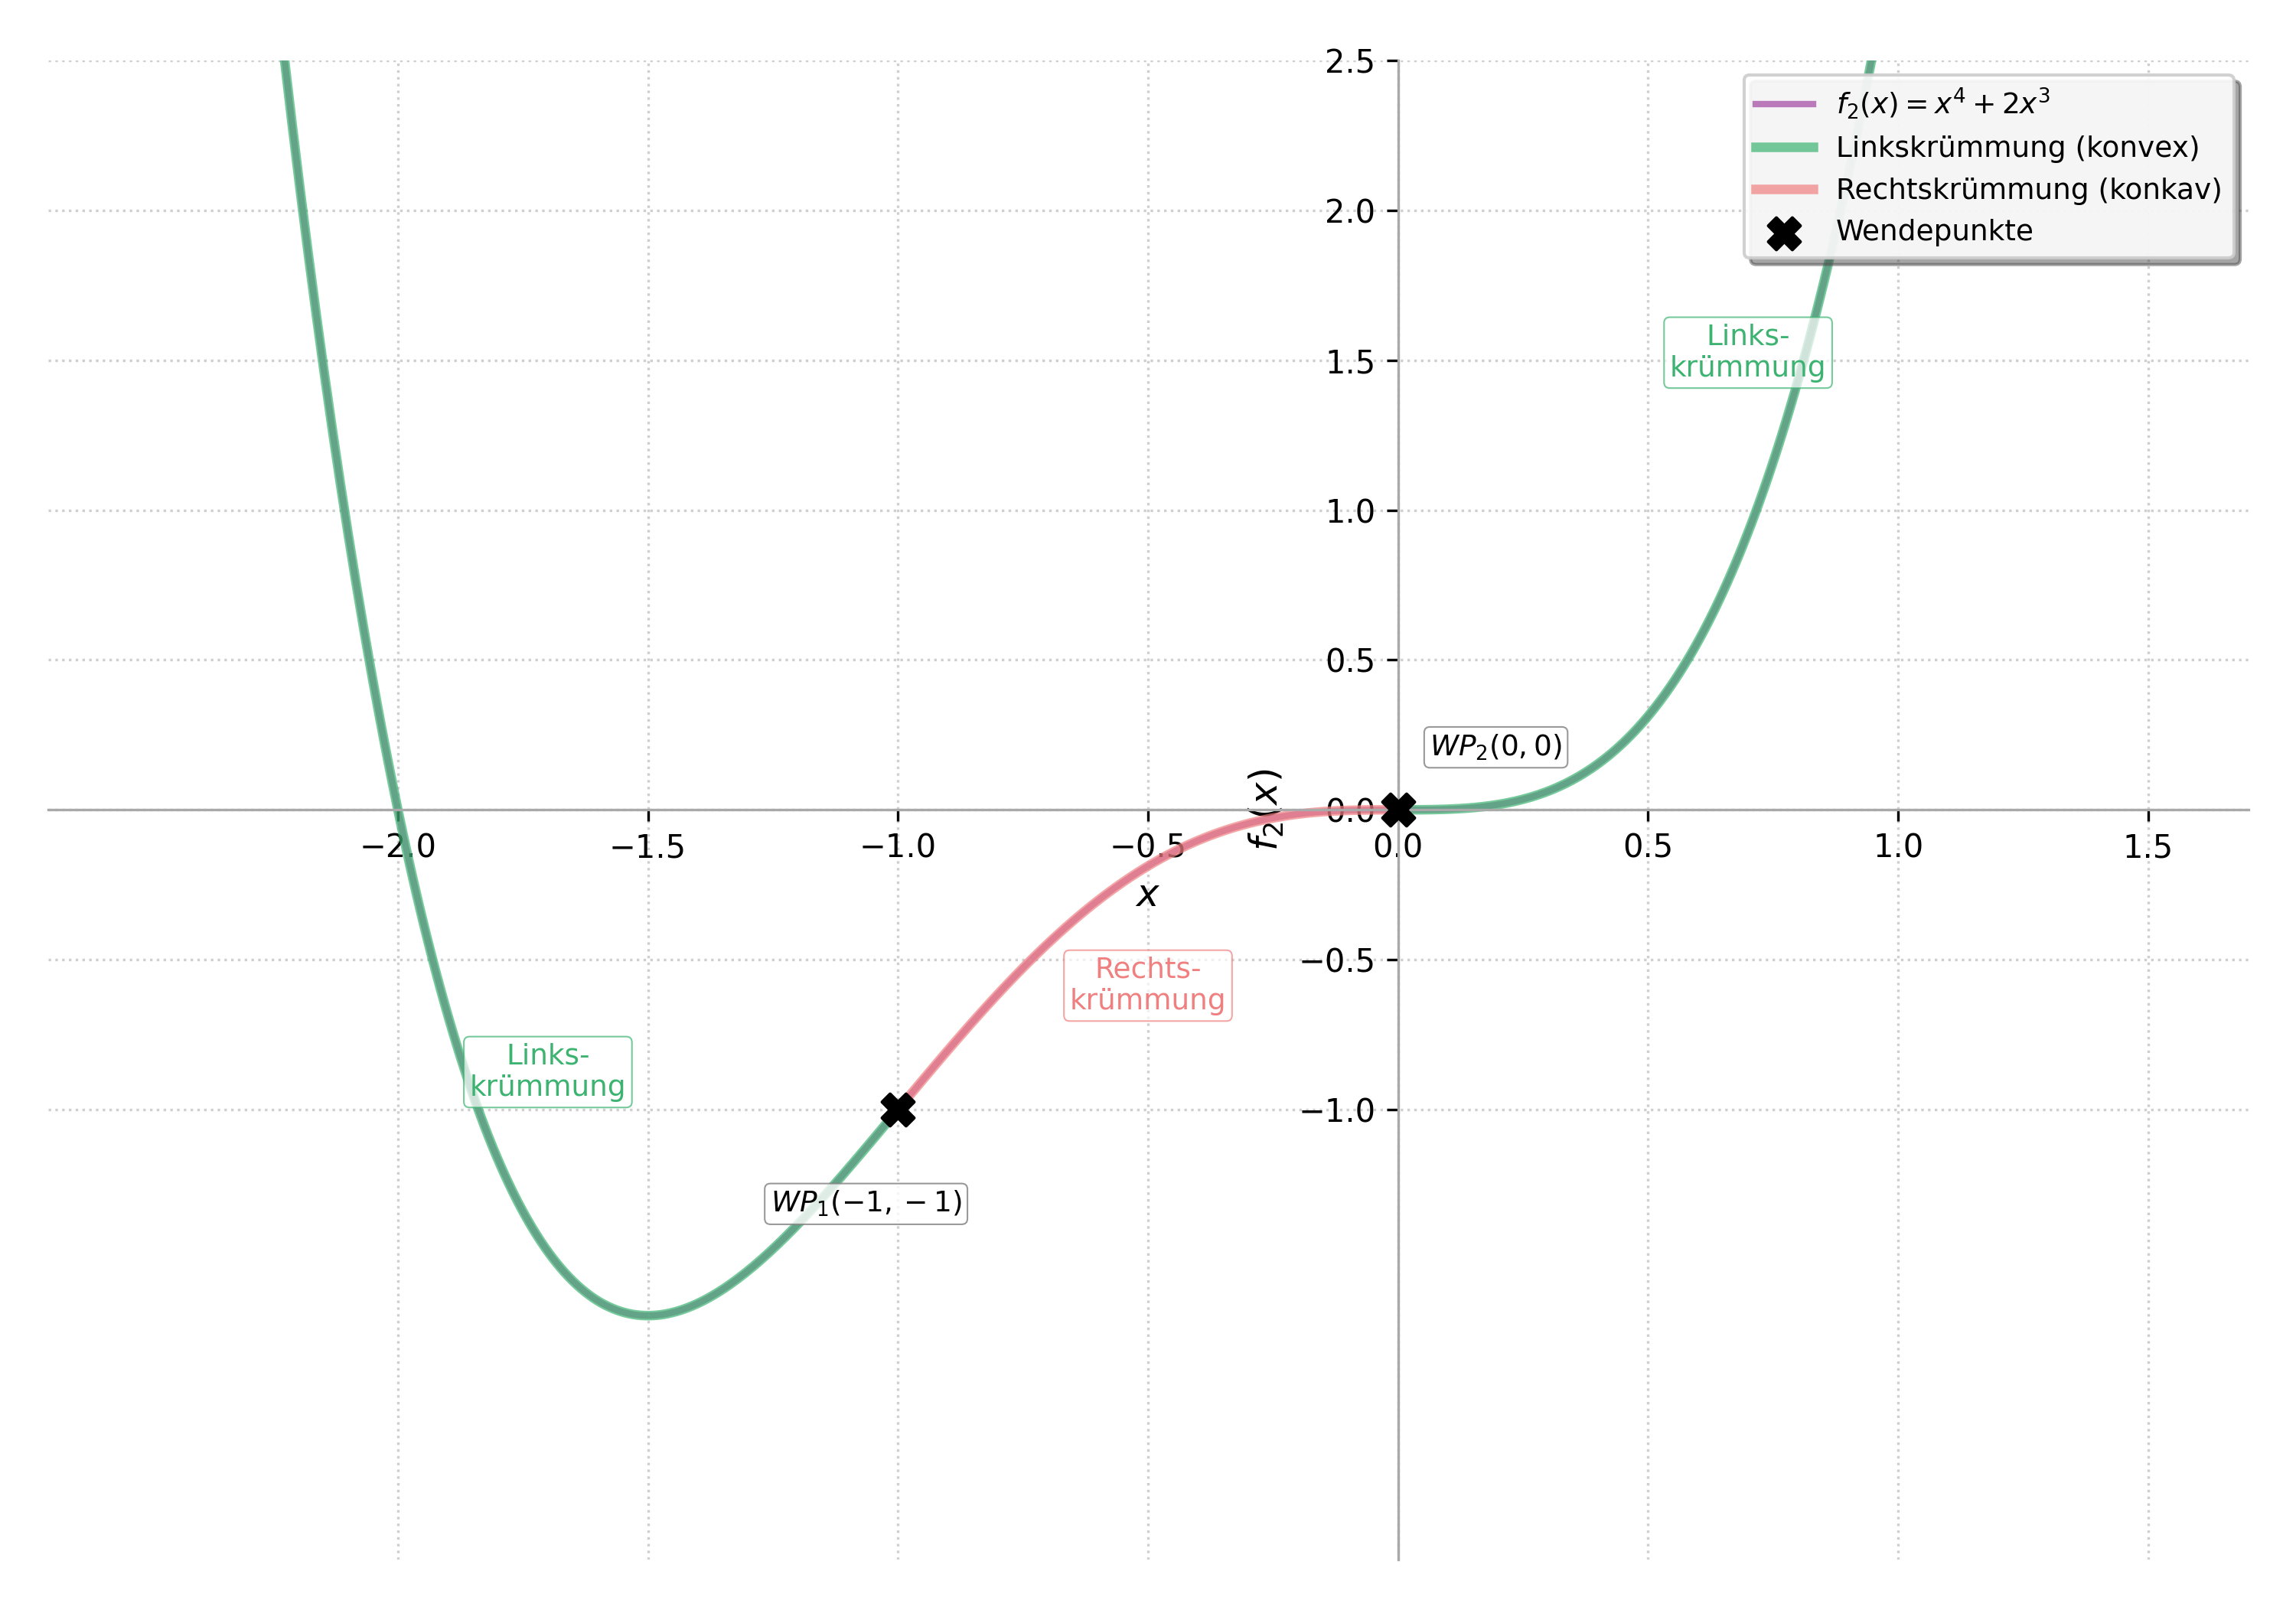
\includegraphics[width=0.8\textwidth]{grafiken/fa_kruemmung_a_pos2.png}
            \captionof{figure}{Grobe Skizze von $f_2(x)=x^4+2x^3$ mit Fokus auf Krümmung (WP bei -1 und 0).}
            \label{fig:fa_kruemmung_a_pos2}
            \end{center}
            \textit{Skizzenbeschreibung:} Der Graph kommt von links oben (Linkskrümmung), hat einen Wendepunkt bei $x=-1$ (Übergang zur Rechtskrümmung), durchläuft einen Bereich mit Rechtskrümmung, hat einen weiteren Wendepunkt bei $x=0$ (Übergang zur Linkskrümmung) und geht dann nach rechts oben weg (Linkskrümmung). Das Globalverhalten ist wie $x^4$.

            \item \textbf{Fall $a=-2$:} $f_{-2}(x) = x^4 - 2x^3$.
            $f_{-2}''(x) = 12x^2 - 12x = 12x(x-1)$.
            Wendestellen bei $x_W_1=0$ und $x_W_2=1$.
            $f_{-2}''(x)$ ist eine nach oben geöffnete Parabel.
            Krümmungsverhalten:
            \begin{itemize}
                \item $(-\infty, 0)$: $f_{-2}''(x) > 0 \Rightarrow$ Linkskrümmung.
                \item $(0, 1)$: $f_{-2}''(x) < 0 \Rightarrow$ Rechtskrümmung.
                \item $(1, \infty)$: $f_{-2}''(x) > 0 \Rightarrow$ Linkskrümmung.
            \end{itemize}
            \begin{center}
            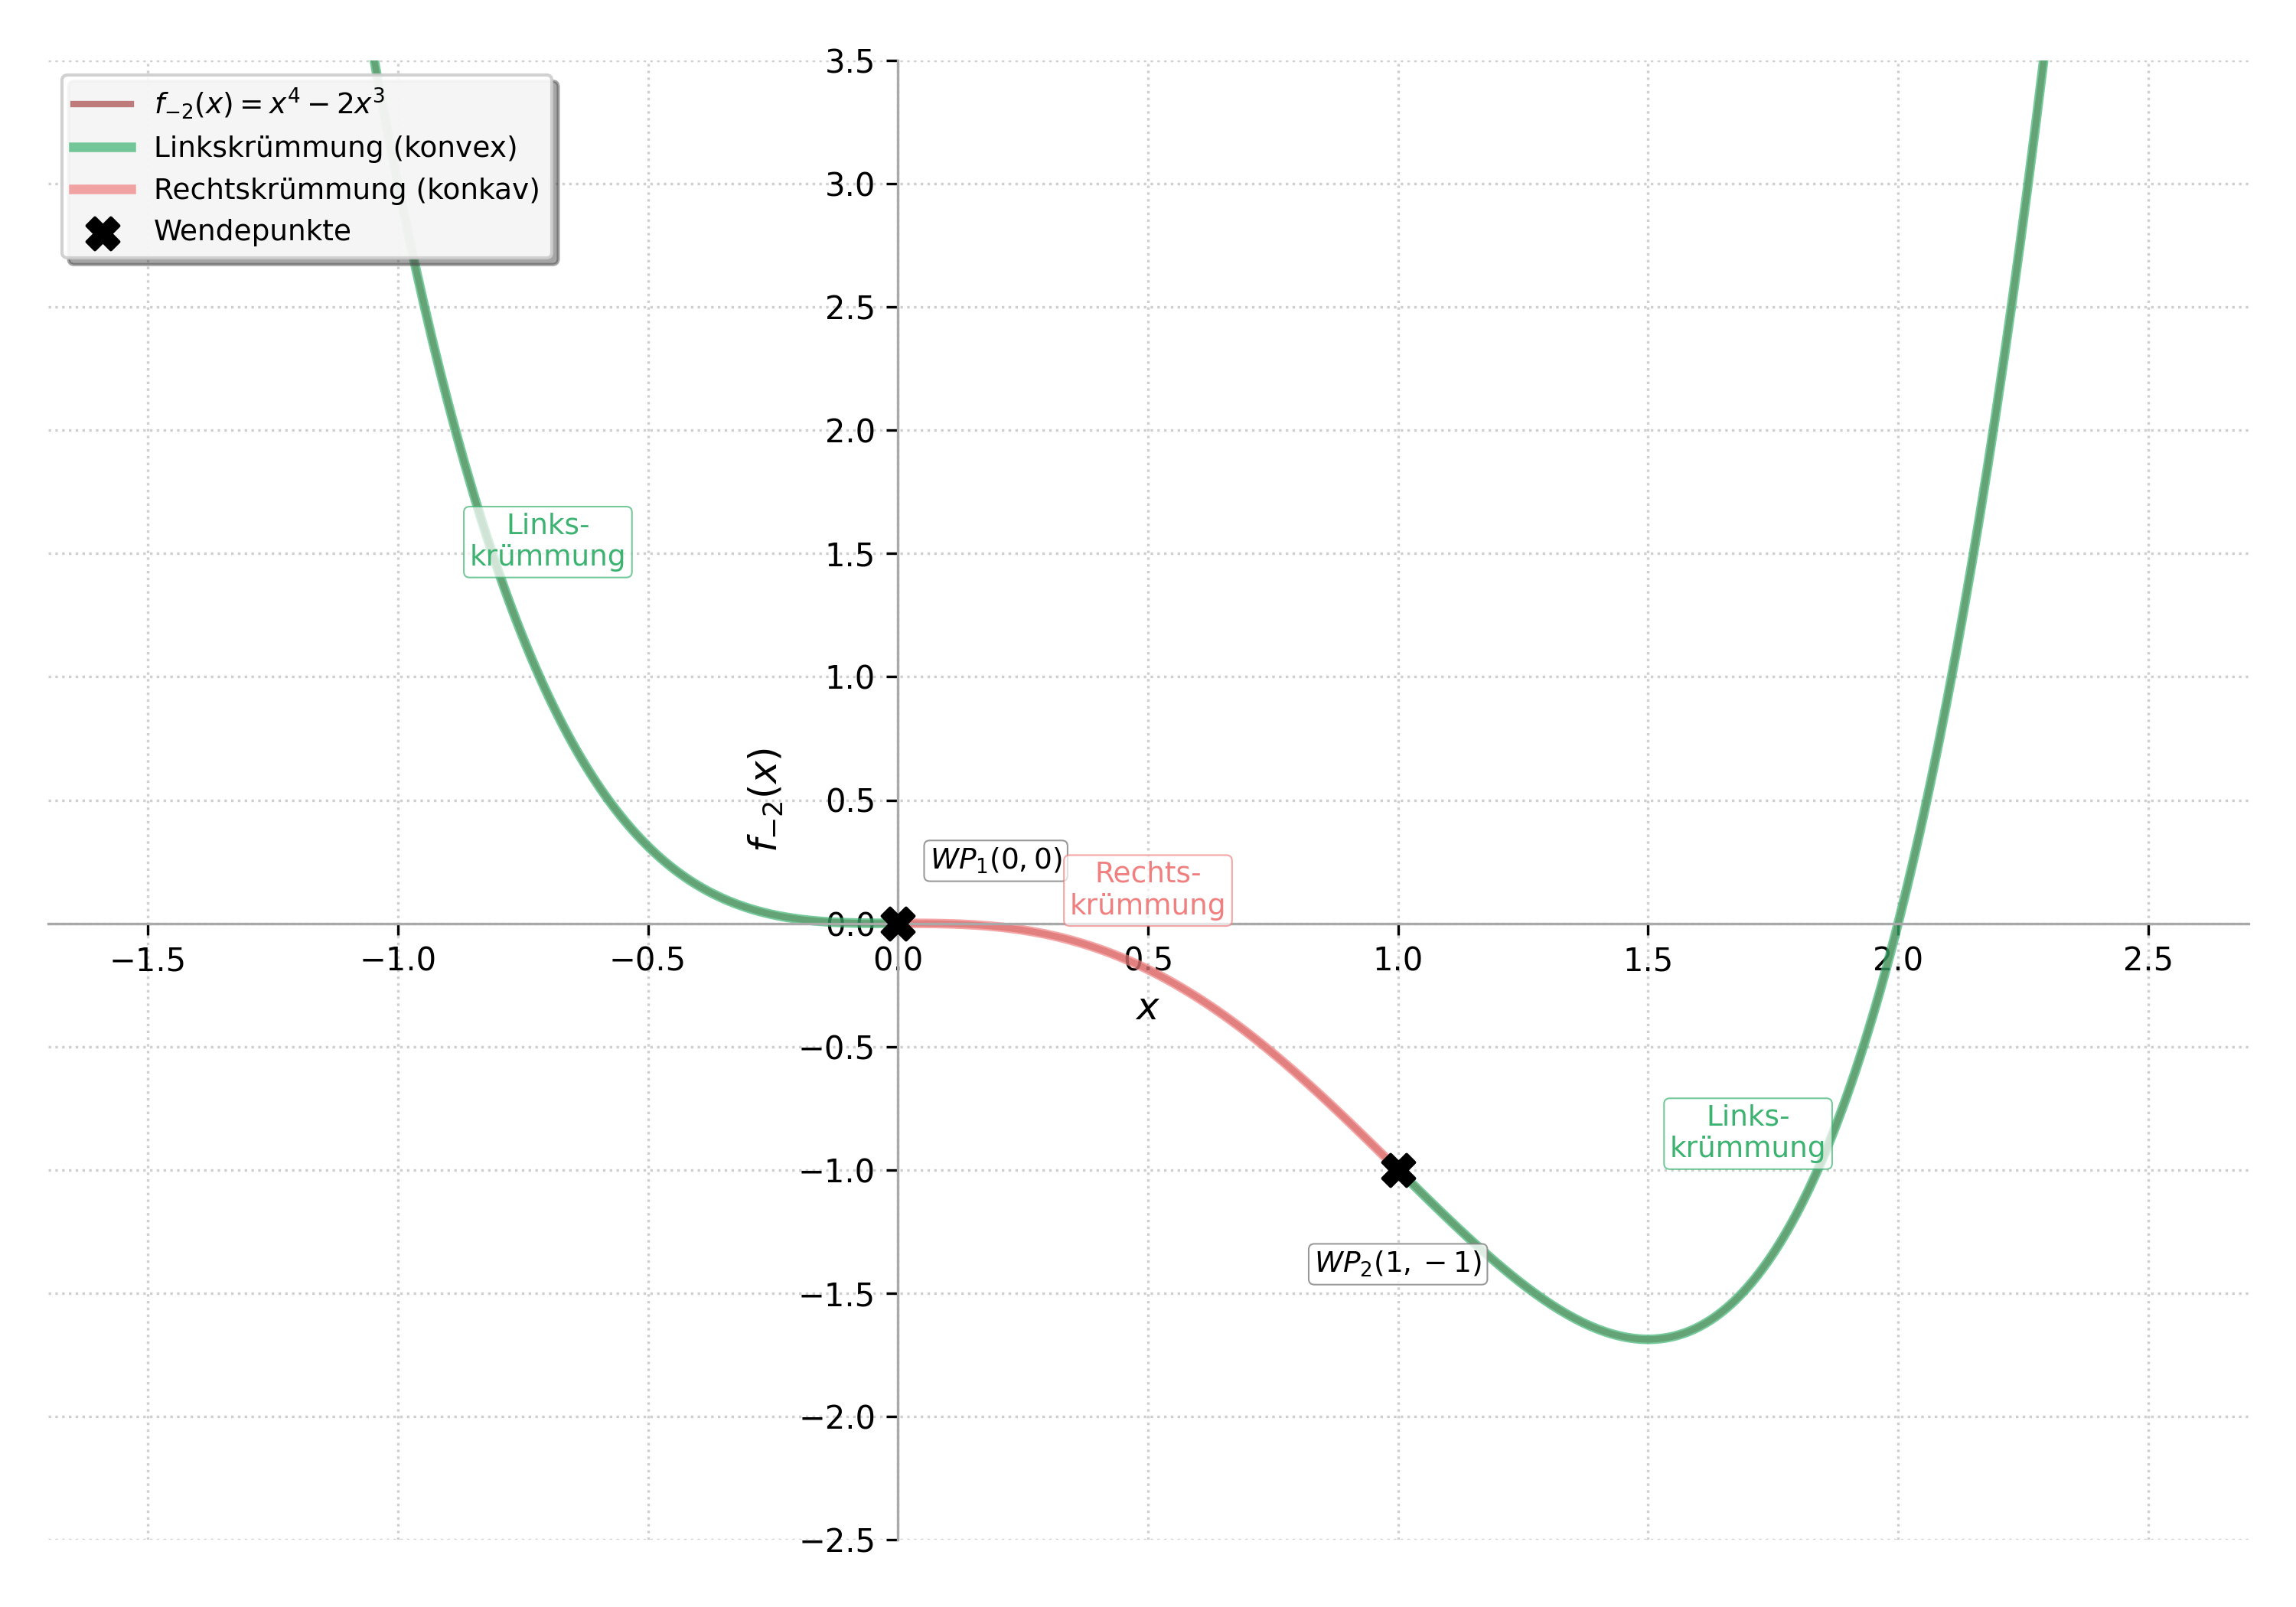
\includegraphics[width=0.8\textwidth]{grafiken/fa_kruemmung_a_neg2.png}
            \captionof{figure}{Grobe Skizze von $f_{-2}(x)=x^4-2x^3$ mit Fokus auf Krümmung (WP bei 0 und 1).}
            \label{fig:fa_kruemmung_a_neg2}
            \end{center}
            \textit{Skizzenbeschreibung:} Der Graph kommt von links oben (Linkskrümmung), hat einen Wendepunkt bei $x=0$ (Übergang zur Rechtskrümmung), durchläuft einen Bereich mit Rechtskrümmung, hat einen weiteren Wendepunkt bei $x=1$ (Übergang zur Linkskrümmung) und geht dann nach rechts oben weg (Linkskrümmung). Das Globalverhalten ist wie $x^4$.
        \end{itemize}
    \end{itemize}
\end{enumerate}

\end{loesungsumgebung}


\begin{aufgabenumgebung}{Tangenten und Normalen bestimmen – Vielfältige Aufgaben}
\begin{enumerate}
    \item Gegeben ist die Funktion $f(x) = \frac{1}{4}x^4 - x^2 + 1$.
        \begin{itemize}
            \item Bestimme die Gleichung der Tangente und der Normalen an den Graphen von $f$ an der Stelle $x_0 = 2$.
            \item An welchen Stellen $x$ hat der Graph von $f$ eine Tangente mit der Steigung $m=0$? Was für Punkte sind das?
            \item (Schwer): Gibt es eine Tangente an den Graphen von $f$, die parallel zur Geraden $y = -2x+5$ ist? Wenn ja, bestimme die Berührpunkte und die Gleichungen dieser Tangenten.
        \end{itemize}
    \item Gegeben ist die Funktion $g(x) = x^3 - 3x$.
        \begin{itemize}
            \item Bestimme die Wendepunkt(e) von $g(x)$.
            \item Bestimme die Gleichung der Wendetangente(n).
            \item Zeige, dass die Wendetangente im Ursprung (falls vorhanden) die x-Achse nur im Ursprung schneidet.
        \end{itemize}
    \item \textbf{Orthogonale Tangenten (Für Experten):}
        Gegeben ist die Parabel $f(x) = x^2$. Gibt es zwei Punkte $P_1(x_1|f(x_1))$ und $P_2(x_2|f(x_2))$ auf der Parabel, deren Tangenten sich senkrecht schneiden und deren x-Koordinaten die Bedingung $x_1 \cdot x_2 = -1/4$ erfüllen?

    \item \textbf{Normale durch den Ursprung:}
        Für die Funktion $f(x) = \frac{1}{2}x^2 - 2x + 3$, bestimme den Punkt $P(x_0|f(x_0))$ auf dem Graphen, dessen Normale durch den Ursprung $(0|0)$ verläuft.

    \item \textbf{Wendetangente mit speziellen Eigenschaften (Schwer):}
        Gegeben ist die Funktion $f(x) = \frac{1}{6}x^3 - x^2 + 2x + 1$.
        \begin{itemize}
            \item Bestimme die Koordinaten des Wendepunktes $W$.
            \item Bestimme die Gleichung der Wendetangente $t_W(x)$ und der Wendenormalen $n_W(x)$.
            \item Die Wendetangente, die Wendenormale und die y-Achse bilden ein Dreieck. Berechne den Flächeninhalt dieses Dreiecks.
            \item Unter welchem Winkel schneidet die Wendetangente die x-Achse? (Tipp: Der Tangens des Steigungswinkels $\alpha$ einer Geraden ist gleich ihrer Steigung $m$, also $\tan(\alpha) = m$. Du suchst $\alpha = \arctan(m)$.)
        \end{itemize}

    \item \textbf{Berührbedingung und Parameter (Schwer):}
        Gegeben sind die Funktionen $f(x) = x^2 + 2x + 2$ und die Geradenschar $g_k(x) = kx - 2$ (wobei $k \in \mathbb{R}$ ein Parameter ist).
        \begin{itemize}
            \item Für welchen Wert von $k$ berührt die Gerade $g_k(x)$ die Parabel $f(x)$?
            \item Bestimme den Berührpunkt und die Gleichung der gemeinsamen Tangente für diesen Wert von $k$.
            \item (Für Experten): Gibt es einen Wert für $k$, sodass die Gerade $g_k(x)$ eine Normale zur Parabel $f(x)$ an einem Punkt $P(x_0|f(x_0))$ ist? Wenn ja, bestimme $k$ und den Punkt $P$.
        \end{itemize}
\end{enumerate}
\end{aufgabenumgebung}

\begin{loesungsumgebung}[loes:tangenten-normalen-vielfalt]{Tangenten und Normalen bestimmen – Vielfältige Aufgaben}
Zur Bestimmung von Tangenten- und Normalengleichungen verwenden wir die Punkt-Steigungs-Form: $y - y_0 = m(x - x_0)$. Die Tangentensteigung $m_t$ an der Stelle $x_0$ ist $f'(x_0)$, die Normalensteigung $m_n = -1/f'(x_0)$ (falls $f'(x_0) \neq 0$).

\begin{enumerate}[label=(\alph*)]
    \item Gegeben ist die Funktion $f(x) = \frac{1}{4}x^4 - x^2 + 1$.
    Die erste Ableitung ist $f'(x) = x^3 - 2x$.
    \begin{itemize}
        \item \textbf{Tangente und Normale an $x_0 = 2$:}
        Der Berührpunkt ist $P(x_0|f(x_0))$.
        $f(2) = \frac{1}{4}(2)^4 - (2)^2 + 1 = \frac{16}{4} - 4 + 1 = 4 - 4 + 1 = 1$. Also $P(2|1)$.
        Die Tangentensteigung ist $m_t = f'(2) = (2)^3 - 2(2) = 8 - 4 = 4$.
        \textit{Tangentengleichung:} $y - 1 = 4(x - 2) \Rightarrow y = 4x - 8 + 1 \Rightarrow \mathbf{y_t = 4x - 7}$.
        Die Normalensteigung ist $m_n = -1/m_t = -1/4$.
        \textit{Normalengleichung:} $y - 1 = -\frac{1}{4}(x - 2) \Rightarrow y = -\frac{1}{4}x + \frac{2}{4} + 1 \Rightarrow \mathbf{y_n = -\frac{1}{4}x + \frac{3}{2}}$.

        \item \textbf{Stellen $x$ mit Tangentensteigung $m=0$:}
        Wir setzen $f'(x) = 0$:
        $x^3 - 2x = 0 \Rightarrow x(x^2 - 2) = 0$.
        Lösungen: $x_1 = 0$.
        $x^2 - 2 = 0 \Rightarrow x^2 = 2 \Rightarrow x_{2,3} = \pm\sqrt{2}$.
        Die Stellen sind $\mathbf{x=0, x=\sqrt{2}, x=-\sqrt{2}}$. An diesen Stellen hat der Graph waagerechte Tangenten (Kandidaten für lokale Extrema).

        \item \textbf{(Schwer) Tangente parallel zu $y = -2x+5$:}
        Die Steigung der gesuchten Tangente muss $m=-2$ sein. Wir setzen $f'(x) = -2$:
        $x^3 - 2x = -2 \Rightarrow x^3 - 2x + 2 = 0$.
        Dies ist eine kubische Gleichung. Durch Testen von ganzzahligen Teilern des konstanten Glieds ($\pm 1, \pm 2$) finden wir keine einfachen Lösungen:
        $P(1) = 1-2+2 = 1 \neq 0$
        $P(-1) = -1+2+2 = 3 \neq 0$
        $P(2) = 8-4+2 = 6 \neq 0$
        $P(-2) = -8+4+2 = -2 \neq 0$
        Es gibt eine reelle Lösung für diese Gleichung (z.B. durch numerische Verfahren oder den Zwischenwertsatz, da $P(-2)=-2$ und $P(-1)=3$, liegt eine Nullstelle $x_B$ zwischen $-2$ und $-1$, ca. $x_B \approx -1.769$).
        Wenn $x_B$ diese Lösung ist, dann ist der Berührpunkt $(x_B | f(x_B))$ und die Tangentengleichung $y = -2(x-x_B) + f(x_B)$. Eine exakte algebraische Lösung für $x_B$ ist ohne weitere Methoden (wie Cardano-Formel oder Polynomdivision nach Erraten einer rationalen Nullstelle, die hier nicht offensichtlich ist) schwierig.
    \end{itemize}

    \item Gegeben ist die Funktion $g(x) = x^3 - 3x$.
    $g'(x) = 3x^2 - 3$.
    $g''(x) = 6x$.
    $g'''(x) = 6$.
    \begin{itemize}
        \item \textbf{Wendepunkt(e) von $g(x)$:}
        Notwendige Bedingung: $g''(x) = 0 \Rightarrow 6x = 0 \Rightarrow x_W = 0$.
        Hinreichende Bedingung: $g'''(x_W) \neq 0$. $g'''(0) = 6 \neq 0$.
        Also liegt bei $x_W=0$ ein Wendepunkt.
        $y_W = g(0) = 0^3 - 3(0) = 0$.
        Der Wendepunkt ist $\mathbf{W(0|0)}$.
        \item \textbf{Gleichung der Wendetangente(n):}
        Steigung im Wendepunkt: $m_W = g'(0) = 3(0)^2 - 3 = -3$.
        Tangentengleichung durch $W(0|0)$ mit $m_W = -3$:
        $y - 0 = -3(x - 0) \Rightarrow \mathbf{y_W = -3x}$.
        \item \textbf{Zeige, dass die Wendetangente im Ursprung die x-Achse nur im Ursprung schneidet:}
        Die Wendetangente ist $y_W = -3x$. Um den Schnittpunkt mit der x-Achse zu finden, setzen wir $y_W=0$:
        $0 = -3x \Rightarrow x = 0$.
        Der einzige Schnittpunkt mit der x-Achse ist $(0|0)$, also der Ursprung.
    \end{itemize}

    \item \textbf{Orthogonale Tangenten (Für Experten):}
    Gegeben ist $f(x) = x^2$. Die Ableitung ist $f'(x) = 2x$.
    Die Steigungen der Tangenten an den Punkten $P_1(x_1|f(x_1))$ und $P_2(x_2|f(x_2))$ sind $m_1 = f'(x_1) = 2x_1$ und $m_2 = f'(x_2) = 2x_2$.
    Zwei Geraden sind orthogonal, wenn das Produkt ihrer Steigungen $m_1 \cdot m_2 = -1$ ist (vorausgesetzt $m_1, m_2 \neq 0$, also $x_1, x_2 \neq 0$).
    Also: $(2x_1)(2x_2) = -1 \Rightarrow 4x_1x_2 = -1 \Rightarrow x_1x_2 = -\frac{1}{4}$.
    Die in der Aufgabe gegebene Bedingung $x_1 \cdot x_2 = -1/4$ ist genau die Bedingung dafür, dass sich die Tangenten senkrecht schneiden (unter der Annahme $x_1, x_2 \neq 0$).
    \textbf{Ja}, es gibt solche Punktepaare. Für jedes $x_1 \neq 0$ kann man $x_2 = -1/(4x_1)$ wählen (dann ist auch $x_2 \neq 0$), und die Tangenten in $P_1$ und $P_2$ sind orthogonal.

    \item \textbf{Normale durch den Ursprung:}
    Für $f(x) = \frac{1}{2}x^2 - 2x + 3$. $f'(x) = x - 2$.
    Sei $P(x_0|f(x_0))$ der Punkt auf dem Graphen. $y_0 = \frac{1}{2}x_0^2 - 2x_0 + 3$.
    Steigung der Tangente in $P$: $m_t = f'(x_0) = x_0 - 2$.
    Wenn $x_0=2$, ist $m_t=0$, die Tangente $y=f(2)=1$ ist horizontal, die Normale $x=2$ verläuft nicht durch den Ursprung. Also $x_0 \neq 2$.
    Steigung der Normale: $m_n = -\frac{1}{x_0-2}$.
    Die Normale geht durch $P(x_0|y_0)$ und den Ursprung $(0|0)$. Die Steigung der Normalen ist auch $\frac{y_0-0}{x_0-0} = \frac{y_0}{x_0}$ (für $x_0 \neq 0$).
    Also: $\frac{y_0}{x_0} = -\frac{1}{x_0-2}$.
    $y_0(x_0-2) = -x_0$.
    $(\frac{1}{2}x_0^2 - 2x_0 + 3)(x_0-2) = -x_0$.
    $\frac{1}{2}x_0^3 - x_0^2 - 2x_0^2 + 4x_0 + 3x_0 - 6 = -x_0$.
    $\frac{1}{2}x_0^3 - 3x_0^2 + 7x_0 - 6 = -x_0$.
    $\frac{1}{2}x_0^3 - 3x_0^2 + 8x_0 - 6 = 0 \quad | \cdot 2$.
    $x_0^3 - 6x_0^2 + 16x_0 - 12 = 0$.
    Dies ist eine kubische Gleichung. Durch Probieren (z.B. Teiler von 12: $\pm 1, \pm 2, \pm 3, \pm 4, \pm 6, \pm 12$) findet man keine einfache ganzzahlige Lösung. (z.B. $x_0=1 \Rightarrow 1-6+16-12 = -1 \neq 0$). Es existiert mindestens eine reelle Lösung (z.B. $x_0 \approx 0.916$). Ohne eine leicht zu erratende Nullstelle oder weitere Techniken ist die exakte Lösung schwierig. Der Punkt $P(x_0|f(x_0))$ muss dann mit dieser Lösung $x_0$ bestimmt werden.

    \item \textbf{Wendetangente mit speziellen Eigenschaften (Schwer):}
    $f(x) = \frac{1}{6}x^3 - x^2 + 2x + 1$.
    $f'(x) = \frac{1}{2}x^2 - 2x + 2$.
    $f''(x) = x - 2$.
    $f'''(x) = 1$.
    \begin{itemize}
        \item \textbf{Koordinaten des Wendepunktes $W$:}
        $f''(x)=0 \Rightarrow x-2=0 \Rightarrow x_W=2$.
        $f'''(2)=1 \neq 0$, also ein Wendepunkt.
        $y_W = f(2) = \frac{1}{6}(2)^3 - (2)^2 + 2(2) + 1 = \frac{8}{6} - 4 + 4 + 1 = \frac{4}{3} + 1 = \frac{7}{3}$.
        $\mathbf{W(2 | 7/3)}$.
        \item \textbf{Gleichung der Wendetangente $t_W(x)$ und der Wendenormalen $n_W(x)$:}
        Steigung der Wendetangente: $m_t = f'(2) = \frac{1}{2}(2)^2 - 2(2) + 2 = 2 - 4 + 2 = 0$.
        Wendetangente $t_W(x)$: $y - \frac{7}{3} = 0(x-2) \Rightarrow \mathbf{y = \frac{7}{3}}$.
        Wendenormale $n_W(x)$: Da die Tangente horizontal ist, ist die Normale vertikal: $\mathbf{x = 2}$.
        \item \textbf{Flächeninhalt des Dreiecks (Wendetangente, Wendenormale, y-Achse):}
        Die Geraden sind $L_1: y=7/3$ (Tangente), $L_2: x=2$ (Normale), $L_3: x=0$ (y-Achse).
        Schnittpunkte:
        $V_1 = L_1 \cap L_2 = (2, 7/3)$ (Dies ist der Wendepunkt $W$).
        $V_2 = L_1 \cap L_3 = (0, 7/3)$.
        Die Geraden $L_2: x=2$ und $L_3: x=0$ sind parallel und schneiden sich nicht. Somit bilden diese drei Geraden kein geschlossenes Dreieck im üblichen Sinne mit drei Eckpunkten.
        Wenn das Dreieck durch den Wendepunkt $W(2, 7/3)$, den y-Achsenabschnitt der Tangente $P_y(0, 7/3)$ und den Schnittpunkt der Normalen mit der x-Achse $P_x(2,0)$ gebildet wird, dann handelt es sich um ein rechtwinkliges Dreieck mit den Kathetenlängen $2$ (Differenz der x-Koordinaten von $P_y$ und $W$) und $7/3$ (Differenz der y-Koordinaten von $P_x$ und $W$).
        Fläche $A = \frac{1}{2} \cdot \text{Grundseite} \cdot \text{Höhe} = \frac{1}{2} \cdot 2 \cdot \frac{7}{3} = \mathbf{\frac{7}{3}}$ Flächeneinheiten.
        \item \textbf{Winkel der Wendetangente mit der x-Achse:}
        Die Wendetangente ist $y = 7/3$. Ihre Steigung ist $m_t = 0$.
        Der Steigungswinkel $\alpha$ ist gegeben durch $\tan(\alpha) = m_t$.
        $\tan(\alpha) = 0 \Rightarrow \alpha = \arctan(0) = 0^\circ$ (oder $0$ Radiant).
        Die Wendetangente ist parallel zur x-Achse, der Winkel ist $\mathbf{0^\circ}$.
    \end{itemize}

    \item \textbf{Berührbedingung und Parameter (Schwer):}
    $f(x) = x^2 + 2x + 2$ und Geradenschar $g_k(x) = kx - 2$.
    $f'(x) = 2x + 2$. $g_k'(x) = k$.
    \begin{itemize}
        \item \textbf{Für welchen Wert von $k$ berührt $g_k(x)$ die Parabel $f(x)$?}
        Bedingungen für Berührung an Stelle $x_B$:
        1) $f(x_B) = g_k(x_B) \Rightarrow x_B^2 + 2x_B + 2 = kx_B - 2$.
        2) $f'(x_B) = g_k'(x_B) \Rightarrow 2x_B + 2 = k$.
        Setze (2) in (1) ein:
        $x_B^2 + 2x_B + 2 = (2x_B + 2)x_B - 2$
        $x_B^2 + 2x_B + 2 = 2x_B^2 + 2x_B - 2$
        $0 = x_B^2 - 4 \Rightarrow x_B^2 = 4 \Rightarrow x_B = \pm 2$.
        Wenn $x_B = 2$: $k = 2(2) + 2 = 6$.
        Wenn $x_B = -2$: $k = 2(-2) + 2 = -4 + 2 = -2$.
        Die Werte sind $\mathbf{k=6}$ und $\mathbf{k=-2}$.
        \item \textbf{Berührpunkt und Gleichung der gemeinsamen Tangente:}
        \begin{itemize}
            \item Für $k=6$: $x_B=2$. $y_B = f(2) = 2^2+2(2)+2 = 10$. Berührpunkt $\mathbf{B_1(2|10)}$.
            Gemeinsame Tangente: $g_6(x) = 6x-2$.
            \item Für $k=-2$: $x_B=-2$. $y_B = f(-2) = (-2)^2+2(-2)+2 = 2$. Berührpunkt $\mathbf{B_2(-2|2)}$.
            Gemeinsame Tangente: $g_{-2}(x) = -2x-2$.
        \end{itemize}
        \item \textbf{(Für Experten) $g_k(x)$ als Normale zu $f(x)$:}
        Die Gerade $g_k(x)=kx-2$ soll Normale zu $f(x)$ an einem Punkt $P(x_0|f(x_0))$ sein.
        Steigung der Normale zu $f(x)$ an $x_0$: $m_n = -1/f'(x_0) = -1/(2x_0+2)$ (für $x_0 \neq -1$).
        Also $k = -1/(2x_0+2)$.
        Der Punkt $P(x_0|f(x_0))$ muss auf $g_k(x)$ liegen: $f(x_0) = kx_0 - 2$.
        $x_0^2 + 2x_0 + 2 = \left(-\frac{1}{2x_0+2}\right)x_0 - 2$.
        $(x_0^2 + 2x_0 + 4)(2x_0+2) = -x_0$.
        $2x_0^3 + 2x_0^2 + 4x_0^2 + 4x_0 + 8x_0 + 8 = -x_0$.
        $2x_0^3 + 6x_0^2 + 13x_0 + 8 = 0$.
        Diese kubische Gleichung muss gelöst werden. Eine rationale Nullstelle $x_0=-1/2$ wurde im internen Test nicht gefunden, aber wir prüfen erneut:
        $2(-1/8) + 6(1/4) + 13(-1/2) + 8 = -1/4 + 6/4 - 26/4 + 32/4 = (-1+6-26+32)/4 = 11/4 \neq 0$.
        Testen wir $x_0=-2$: $2(-8)+6(4)+13(-2)+8 = -16+24-26+8 = -10 \neq 0$.
        Testen wir $x_0=-1$: In diesem Fall wäre $f'(x_0)=0$, die Normale $x=-1$. Die Gleichung der Normalen wäre $x=-1$. Die Gerade $g_k(x)=kx-2$ kann nur dann $x=-1$ sein, wenn $k$ undefiniert ist und $-2$ auch, was nicht geht. Also $x_0 \neq -1$.
        Die Gleichung $2x_0^3 + 6x_0^2 + 13x_0 + 8 = 0$ hat eine reelle Lösung (z.B. ist für $x_0=-0.8$, $2(-0.512)+6(0.64)+13(-0.8)+8 = -1.024+3.84-10.4+8 = 0.416$; für $x_0=-0.9$, $2(-0.729)+6(0.81)+13(-0.9)+8 = -1.458+4.86-11.7+8 = -0.298$. Also eine Lösung zwischen -0.9 und -0.8.)
        Die exakte Lösung ist ohne weitere Hilfsmittel schwierig. Wenn eine solche Lösung $x_N$ existiert, dann ist $k = -1/(2x_N+2)$ und der Punkt ist $P(x_N|f(x_N))$.
    \end{itemize}
\end{enumerate}

\end{loesungsumgebung}

\begin{aufgabenumgebung}{Extrempunkte und Sattelpunkte finden und identifizieren}
Untersuche die folgenden Funktionen auf Extrempunkte und Sattelpunkte. Gib jeweils die Koordinaten und die Art des Punktes an. Nutze die notwendigen und hinreichenden Bedingungen.

\begin{enumerate}
    \item $f(x) = x^3 - 3x^2 + 3x + 1$


    \item $g(x) = \frac{1}{4}x^4 - \frac{1}{2}x^2 + 1$

    \item $h(x) = x^5 - \frac{5}{3}x^3$
    \item \textbf{Für Experten:} Konstruiere eine Polynomfunktion $k(x)$ vom Grad 5, die bei $x=0$ einen Sattelpunkt hat und bei $x=2$ einen Tiefpunkt. (Beginne mit den Bedingungen für die Ableitungen.)
\end{enumerate}
\end{aufgabenumgebung}



\begin{loesungsumgebung}[loes:sattelpunkte-identifizieren]{Sattelpunkte finden und identifizieren}
Wir untersuchen die gegebenen Funktionen auf Extrempunkte und Sattelpunkte.

\begin{enumerate}[label=(\alph*)]
    \item \textbf{Funktion $f(x) = x^3 - 3x^2 + 3x + 1$}
    \begin{itemize}
        \item \textbf{Ableitungen:}
        $f'(x) = 3x^2 - 6x + 3$
        $f''(x) = 6x - 6$
        $f'''(x) = 6$
        \item \textbf{Kritische Stellen ($f'(x)=0$):}
        $3x^2 - 6x + 3 = 0 \quad | :3$
        $x^2 - 2x + 1 = 0$
        $(x-1)^2 = 0 \Rightarrow x_E = 1$ (doppelte Nullstelle).
        \item \textbf{Untersuchung der kritischen Stelle $x_E=1$:}
        Mit der zweiten Ableitung: $f''(1) = 6(1) - 6 = 0$. Dieses Kriterium liefert keine Aussage.
        Mit der dritten Ableitung: $f'''(1) = 6 \neq 0$.
        Da $f'(1)=0$, $f''(1)=0$ und $f'''(1) \neq 0$, liegt bei $x=1$ ein \textbf{Sattelpunkt (Terrassenpunkt)} vor.
        \textit{Alternativ mit VZW von $f'(x) = 3(x-1)^2$:}
        Da $(x-1)^2 \ge 0$ für alle $x$, ist $f'(x) = 3(x-1)^2 \ge 0$ für alle $x$.
        Für $x < 1$ (z.B. $x=0$): $f'(0) = 3(-1)^2 = 3 > 0$.
        Für $x > 1$ (z.B. $x=2$): $f'(2) = 3(1)^2 = 3 > 0$.
        Es findet kein Vorzeichenwechsel statt ($+$ nach $+$), was einen Sattelpunkt bestätigt.
        \item \textbf{Koordinaten des Sattelpunkts:}
        $y_E = f(1) = 1^3 - 3(1)^2 + 3(1) + 1 = 1 - 3 + 3 + 1 = 2$.
        $\rightarrow \mathbf{SP(1|2)}$.
        \item \textbf{'Normale' Extrempunkte:} Die Funktion hat keine lokalen Hoch- oder Tiefpunkte, nur einen Sattelpunkt.
    \end{itemize}

    \item \textbf{Funktion $g(x) = \frac{1}{4}x^4 - \frac{1}{2}x^2 + 1$}
    \begin{itemize}
        \item \textbf{Ableitungen:}
        $g'(x) = x^3 - x$
        $g''(x) = 3x^2 - 1$
        \item \textbf{Kritische Stellen ($g'(x)=0$):}
        $x^3 - x = 0 \Rightarrow x(x^2-1) = 0 \Rightarrow x(x-1)(x+1) = 0$.
        Kandidaten: $x_1 = 0$, $x_2 = 1$, $x_3 = -1$.
        \item \textbf{Untersuchung mit $g''(x)$:}
        \begin{itemize}
            \item Für $x_1 = 0$: $g''(0) = 3(0)^2 - 1 = -1 < 0 \Rightarrow$ Lokaler Hochpunkt.
            $y_1 = g(0) = 1$. Punkt: $\mathbf{HP(0|1)}$.
            \item Für $x_2 = 1$: $g''(1) = 3(1)^2 - 1 = 2 > 0 \Rightarrow$ Lokaler Tiefpunkt.
            $y_2 = g(1) = \frac{1}{4} - \frac{1}{2} + 1 = \frac{3}{4}$. Punkt: $\mathbf{TP(1|3/4)}$.
            \item Für $x_3 = -1$: $g''(-1) = 3(-1)^2 - 1 = 2 > 0 \Rightarrow$ Lokaler Tiefpunkt.
            $y_3 = g(-1) = \frac{1}{4} - \frac{1}{2} + 1 = \frac{3}{4}$. Punkt: $\mathbf{TP(-1|3/4)}$.
        \end{itemize}
        \item \textbf{Sattelpunkte:} Da für alle kritischen Stellen $g''(x_E) \neq 0$ war, gibt es keine Sattelpunkte. Die Nullstellen von $g''(x)$ sind $x = \pm 1/\sqrt{3}$, diese sind aber keine Nullstellen von $g'(x)$.
    \end{itemize}

    \item \textbf{Funktion $h(x) = x^5 - \frac{5}{3}x^3$}
    \begin{itemize}
        \item \textbf{Ableitungen:}
        $h'(x) = 5x^4 - 5x^2$
        $h''(x) = 20x^3 - 10x$
        $h'''(x) = 60x^2 - 10$
        \item \textbf{Kritische Stellen ($h'(x)=0$):}
        $5x^4 - 5x^2 = 0 \Rightarrow 5x^2(x^2-1) = 0 \Rightarrow 5x^2(x-1)(x+1) = 0$.
        Kandidaten: $x_1 = 0$ (doppelte Nullstelle), $x_2 = 1$, $x_3 = -1$.
        \item \textbf{Untersuchung der kritischen Stellen:}
        \begin{itemize}
            \item \textbf{Für $x_1 = 0$:}
            $h''(0) = 20(0)^3 - 10(0) = 0$.
            $h'''(0) = 60(0)^2 - 10 = -10 \neq 0$.
            Da $h'(0)=0, h''(0)=0$ und $h'''(0) \neq 0$, liegt bei $x=0$ ein \textbf{Sattelpunkt} vor.
            $y_1 = h(0) = 0$. Punkt: $\mathbf{SP(0|0)}$.
            \item \textbf{Für $x_2 = 1$:}
            $h''(1) = 20(1)^3 - 10(1) = 20 - 10 = 10 > 0 \Rightarrow$ Lokaler Tiefpunkt.
            $y_2 = h(1) = 1^5 - \frac{5}{3}(1)^3 = 1 - \frac{5}{3} = -\frac{2}{3}$. Punkt: $\mathbf{TP(1|-2/3)}$.
            \item \textbf{Für $x_3 = -1$:}
            $h''(-1) = 20(-1)^3 - 10(-1) = -20 + 10 = -10 < 0 \Rightarrow$ Lokaler Hochpunkt.
            $y_3 = h(-1) = (-1)^5 - \frac{5}{3}(-1)^3 = -1 + \frac{5}{3} = \frac{2}{3}$. Punkt: $\mathbf{HP(-1|2/3)}$.
        \end{itemize}
        \item Die Funktion hat sowohl Extrempunkte (HP bei $x=-1$, TP bei $x=1$) als auch einen Sattelpunkt (bei $x=0$).
    \end{itemize}

 
    \item \textbf{Für Experten: Konstruktion einer Polynomfunktion $k(x)$ vom Grad 5}
    Gesucht: $k(x)$ mit Sattelpunkt bei $x=0$ und Tiefpunkt bei $x=2$.
    Bedingungen:
    \begin{itemize}
        \item Sattelpunkt bei $x=0$: $k'(0)=0$, $k''(0)=0$, $k'''(0) \neq 0$.
        \item Tiefpunkt bei $x=2$: $k'(2)=0$, $k''(2) > 0$.
    \end{itemize}
    Sei $k(x) = ax^5 + bx^4 + cx^3 + dx^2 + ex + f$.
    \begin{itemize}
        \item $k'(x) = 5ax^4 + 4bx^3 + 3cx^2 + 2dx + e$.
        \item $k''(x) = 20ax^3 + 12bx^2 + 6cx + 2d$.
        \item $k'''(x) = 60ax^2 + 24bx + 6c$.
    \end{itemize}
    Aus den Bedingungen für den Sattelpunkt bei $x=0$:
    \begin{itemize}
        \item $k'(0)=0 \Rightarrow e=0$.
        \item $k''(0)=0 \Rightarrow 2d=0 \Rightarrow d=0$.
        \item $k'''(0) \neq 0 \Rightarrow 6c \neq 0 \Rightarrow c \neq 0$.
    \end{itemize}
    Also ist $k'(x) = 5ax^4 + 4bx^3 + 3cx^2$. (Die Konstante $f$ in $k(x)$ spielt für die Ableitungen keine Rolle, wir können $f=0$ setzen.)
    Aus den Bedingungen für den Tiefpunkt bei $x=2$:
    \begin{itemize}
        \item $k'(2)=0 \Rightarrow 5a(16) + 4b(8) + 3c(4) = 0 \Rightarrow 80a + 32b + 12c = 0 \Rightarrow \mathbf{20a + 8b + 3c = 0}$ (G1)
        \item $k''(2)>0 \Rightarrow 20a(8) + 12b(4) + 6c(2) > 0 \Rightarrow 160a + 48b + 12c > 0 \Rightarrow \mathbf{40a + 12b + 3c > 0}$ (U1)
    \end{itemize}
    Wir wählen $c=1$ (erfüllt $c \neq 0$).
    (G1): $20a + 8b + 3 = 0 \Rightarrow 8b = -20a - 3 \Rightarrow b = -\frac{5}{2}a - \frac{3}{8}$.
    Setze $b$ in (U1) ein:
    $40a + 12(-\frac{5}{2}a - \frac{3}{8}) + 3 > 0$
    $40a - 30a - \frac{36}{8} + 3 > 0$
    $10a - \frac{9}{2} + \frac{6}{2} > 0 \Rightarrow 10a - \frac{3}{2} > 0 \Rightarrow 10a > \frac{3}{2} \Rightarrow a > \frac{3}{20}$.
    Wählen wir den einfachsten Wert $a=1$ (ist $>\frac{3}{20}$).
    Dann $b = -\frac{5}{2}(1) - \frac{3}{8} = -\frac{20}{8} - \frac{3}{8} = -\frac{23}{8}$.
    Die Koeffizienten sind $a=1, b=-23/8, c=1, d=0, e=0, f=0$.
    Eine mögliche Funktion ist: $\mathbf{k(x) = x^5 - \frac{23}{8}x^4 + x^3}$.\\
    \textit{Hinweis:} Diese Funktion erfüllt die lokalen Bedingungen. Sie hat jedoch eine weitere kritische Stelle bei $x=3/10$, die ein lokales Maximum darstellt. Eine Funktion 5. Grades zu konstruieren, die \textit{ausschließlich} einen Sattelpunkt bei $x=0$ und einen Tiefpunkt bei $x=2$ als kritische Punkte hat, ist deutlich komplexer und würde erfordern, dass die Ableitung $k'(x)$ nur bei $0$ und $2$ Nullstellen der passenden Art hat. Der gewählte Ansatz erfüllt die Bedingungen an den spezifizierten Stellen.


\end{enumerate}

\end{loesungsumgebung}


\begin{aufgabenumgebung}{Nullstellen finden – Übung und Vertiefung}
Berechne die Nullstellen der folgenden Funktionen. Entscheide selbst, welche Methode (Ausklammern, p-q-Formel, Mitternachtsformel, Substitution, Polynomdivision nach Raten einer Nullstelle) am besten geeignet ist. Überprüfe bei quadratischen Gleichungen immer zuerst die Diskriminante, um die Anzahl der erwarteten reellen Nullstellen zu bestimmen.
\begin{enumerate}
    \item $f(x) = x^2 - x - 6$


    \item $g(x) = -2x^2 + 12x - 18$ 


    \item $h(x) = x^2 + 2x + 5$



    \item $k(x) = 3x^2 - 12$ 


    \item $m(x) = -0.5x^2 + 2x$


    \item \textbf{Polynom 3. Grades durch Ausklammern:}
        $p(x) = x^3 - 5x^2 + 6x$


    \item \textbf{Biquadratische Funktion:}
        $q(x) = x^4 - 10x^2 + 9$


    \item \textbf{Produkt aus Linearfaktoren (versteckt):}
        $r(x) = (x^2-4)(x^2+x-2)$


    \item \textbf{Funktion mit bekannter Nullstelle (Polynomdivision anwenden):}
        Gegeben ist die Funktion $s(x) = x^3 - 2x^2 - 5x + 6$. Es ist bekannt, dass $x_1=1$ eine Nullstelle ist. Finde die anderen Nullstellen mithilfe der Polynomdivision.
        \textit{(Vergleiche auch den Tipp mit dem Koeffizientenvergleich aus der vorherigen Version dieser Aufgabe.)}

    \item \textbf{Nullstellen und Parameter:}
        Für welche Werte des Parameters $k$ hat die Funktion $f_k(x) = x^2 - 2kx + (k+2)$ genau eine, zwei oder keine reelle(n) Nullstelle(n)?

    \item \textbf{Anwendung des Satzes von Vieta (Kopfrechnen für Profis):}
        Versuche, die Nullstellen der folgenden quadratischen Funktionen (in Normalform $x^2+px+q=0$) durch 'scharfes Hinsehen' mit dem Satz von Vieta zu finden. Suche also zwei Zahlen $x_1, x_2$, für die gilt: $x_1+x_2 = -p$ und $x_1 \cdot x_2 = q$.
        \begin{enumerate}[label=(\alph*)]
            \item $f(x) = x^2 - 5x + 6$
            \item $g(x) = x^2 + 2x - 8$
            \item $h(x) = x^2 - 7x + 10$
        \end{enumerate}

\end{enumerate}

\end{aufgabenumgebung}


\begin{loesungsumgebung}[loes:nullstellen-uebung-vertiefung-revised]{Nullstellen finden – Übung und Vertiefung}
Wir berechnen die Nullstellen der folgenden Funktionen $f(x)=0$.

\begin{enumerate}[label=(\alph*)]
    \item \textbf{Funktion $f(x) = x^2 - x - 6$} \\
    Quadratische Gleichung mit $a=1, b=-1, c=-6$.
    Diskriminante: $D = b^2 - 4ac = (-1)^2 - 4(1)(-6) = 1 + 24 = 25$.
    Da $D > 0$, gibt es zwei verschiedene reelle Nullstellen.
    Mitternachtsformel: $x_{1,2} = \frac{-(-1) \pm \sqrt{25}}{2(1)} = \frac{1 \pm 5}{2}$.
    $x_1 = \frac{1+5}{2} = 3$, $x_2 = \frac{1-5}{2} = -2$.
    Nullstellen: $\mathbf{x_1=3, x_2=-2}$.

    \item \textbf{Funktion $g(x) = -2x^2 + 12x - 18$} \\
    Quadratische Gleichung mit $a=-2, b=12, c=-18$.
    Diskriminante: $D = b^2 - 4ac = (12)^2 - 4(-2)(-18) = 144 - 144 = 0$.
    Da $D=0$, gibt es genau eine (doppelte) reelle Nullstelle. Der Graph berührt die x-Achse.
    Mitternachtsformel: $x_0 = \frac{-12 \pm \sqrt{0}}{2(-2)} = \frac{-12}{-4} = 3$.
    Nullstelle: $\mathbf{x_0=3}$ (doppelte Nullstelle).

    \item \textbf{Funktion $h(x) = x^2 + 2x + 5$} \\
    Quadratische Gleichung mit $a=1, b=2, c=5$.
    Diskriminante: $D = b^2 - 4ac = (2)^2 - 4(1)(5) = 4 - 20 = -16$.
    Da $D < 0$, gibt es keine reellen Nullstellen. Der Graph schneidet die x-Achse nicht.
    Nullstellen: \textbf{Keine reellen Nullstellen}.

    \item \textbf{Funktion $k(x) = 3x^2 - 12$} \\
    Setze $k(x)=0 \Rightarrow 3x^2 - 12 = 0$. Direkte Auflösung:
    $$
    \begin{array}{r c l c l}
    \umformung{3x^2 - 12}{0}{+}{12}
    \umformung{3x^2}{12}{\div}{3}
    \umformungend{x^2}{4}
    \end{array}
    $$
    Aus $x^2=4$ folgt $x = \pm\sqrt{4}$.
    Nullstellen: $\mathbf{x_1=2, x_2=-2}$.

    \item \textbf{Funktion $m(x) = -0.5x^2 + 2x$} \\
    Setze $m(x)=0 \Rightarrow -0.5x^2 + 2x = 0$. Ausklammern:
    $x(-0.5x + 2) = 0$.
    Nach dem Satz vom Nullprodukt:
    $x_1 = 0$ oder $-0.5x + 2 = 0$.
    Für $-0.5x + 2 = 0$:
    $$
    \begin{array}{r c l c l}
    \umformung{-0.5x + 2}{0}{-}{2}
    \umformung{-0.5x}{-2}{\div}{(-0.5)}
    \umformungend{x_2}{4}
    \end{array}
    $$
    Nullstellen: $\mathbf{x_1=0, x_2=4}$.

    \item \textbf{Polynom 3. Grades: $p(x) = x^3 - 5x^2 + 6x$} \\
    Setze $p(x)=0 \Rightarrow x^3 - 5x^2 + 6x = 0$. Ausklammern:
    $x(x^2 - 5x + 6) = 0$.
    $x_1 = 0$ oder $x^2 - 5x + 6 = 0$.
    Für $x^2 - 5x + 6 = 0$ (vgl. Teil (a) oder Vieta): $p=-5, q=6$. $x_a+x_b=5, x_a x_b=6 \Rightarrow x_a=2, x_b=3$.
    Nullstellen: $\mathbf{x_1=0, x_2=2, x_3=3}$.

    \item \textbf{Biquadratische Funktion: $q(x) = x^4 - 10x^2 + 9$} \\
    Setze $q(x)=0 \Rightarrow x^4 - 10x^2 + 9 = 0$. Substitution: $z = x^2$.
    $z^2 - 10z + 9 = 0$.
    Lösen für $z$ (z.B. Vieta: $z_a+z_b=10, z_a z_b=9 \Rightarrow z_a=1, z_b=9$):
    $z_1 = 1$, $z_2 = 9$.
    Rücksubstitution:
    $x^2 = z_1 \Rightarrow x^2 = 1 \Rightarrow x = \pm 1$.
    $x^2 = z_2 \Rightarrow x^2 = 9 \Rightarrow x = \pm 3$.
    Nullstellen: $\mathbf{x_1=1, x_2=-1, x_3=3, x_4=-3}$.

    \item \textbf{Produkt aus Linearfaktoren (versteckt): $r(x) = (x^2-4)(x^2+x-2)$} \\
    Setze $r(x)=0 \Rightarrow (x^2-4)(x^2+x-2) = 0$. Satz vom Nullprodukt:
    \begin{itemize}
        \item $x^2-4 = 0 \Rightarrow x^2 = 4 \Rightarrow x = \pm 2$.
        \item $x^2+x-2 = 0$. Diskriminante: $D = 1^2 - 4(1)(-2) = 1+8=9$.
        $x = \frac{-1 \pm \sqrt{9}}{2} = \frac{-1 \pm 3}{2}$.
        $x_3 = \frac{-1+3}{2} = 1$. $x_4 = \frac{-1-3}{2} = -2$.
    \end{itemize}
    Die verschiedenen Nullstellen sind $\mathbf{x_1=2, x_2=-2 (\text{doppelt}), x_3=1}$. (Oder $\{-2, 1, 2\}$ als Menge).

    \item \textbf{Funktion mit bekannter Nullstelle (Polynomdivision anwenden): $s(x) = x^3 - 2x^2 - 5x + 6$} \\
    Bekannt ist $x_1=1$ als Nullstelle, also ist $(x-1)$ ein Linearfaktor. Wir führen eine Polynomdivision durch:

    \polyset{style=C, vars=x, div=:} % Setzt den Divisionsoperator auf ':'
    \polylongdiv{x^3-2x^2-5x+6}{x-1}\\
    Die Polynomdivision ergibt $x^2 - x - 6$.
    Nun suchen wir die Nullstellen des quadratischen Terms: $x^2 - x - 6 = 0$.
    Diese Gleichung wurde in Teil (a) gelöst: $x_2=3, x_3=-2$.
    Die Nullstellen von $s(x)$ sind $\mathbf{x_1=1, x_2=3, x_3=-2}$.

    \item \textbf{Nullstellen und Parameter: $f_k(x) = x^2 - 2kx + (k+2)$} \\
    Koeffizienten $a=1, b=-2k, c=(k+2)$.
    Diskriminante $D = (-2k)^2 - 4(1)(k+2) = 4k^2 - 4k - 8$.
    \begin{itemize}
        \item \textbf{Genau eine Nullstelle:} $D=0 \Rightarrow 4k^2 - 4k - 8 = 0 \Rightarrow k^2 - k - 2 = 0$.
        Lösen für $k$: $(k-2)(k+1)=0 \Rightarrow k=2$ oder $k=-1$.
        Für $\mathbf{k=2}$ oder $\mathbf{k=-1}$ gibt es genau eine Nullstelle.
        \item \textbf{Zwei verschiedene Nullstellen:} $D>0 \Rightarrow k^2 - k - 2 > 0$.
        Die Parabel $P(k)=k^2-k-2$ ist nach oben geöffnet mit Nullstellen bei $-1$ und $2$.
        $P(k)>0$ für $\mathbf{k < -1}$ oder $\mathbf{k > 2}$.
        \item \textbf{Keine reellen Nullstellen:} $D<0 \Rightarrow k^2 - k - 2 < 0$.
        $P(k)<0$ für $\mathbf{-1 < k < 2}$.
    \end{itemize}

    \item \textbf{Anwendung des Satzes von Vieta:}
    Gesucht sind zwei Zahlen $x_1, x_2$ mit $x_1+x_2 = -p$ und $x_1 \cdot x_2 = q$.
    \begin{enumerate}[label=(\roman*)]
        \item $f(x) = x^2 - 5x + 6$: $p=-5, q=6$.
        $x_1+x_2 = 5$, $x_1 \cdot x_2 = 6$. Zahlen: $2, 3$. Nullstellen: $\mathbf{x_1=2, x_2=3}$.
        \item $g(x) = x^2 + 2x - 8$: $p=2, q=-8$.
        $x_1+x_2 = -2$, $x_1 \cdot x_2 = -8$. Zahlen: $2, -4$. Nullstellen: $\mathbf{x_1=2, x_2=-4}$.
        \item $h(x) = x^2 - 7x + 10$: $p=-7, q=10$.
        $x_1+x_2 = 7$, $x_1 \cdot x_2 = 10$. Zahlen: $2, 5$. Nullstellen: $\mathbf{x_1=2, x_2=5}$.
    \end{enumerate}
\end{enumerate}

\end{loesungsumgebung}


\begin{aufgabenumgebung}{Kurvendiskussionen von Polynomen}
Führe eine vollständige Kurvendiskussion (alle Punkte der Checkliste) für die folgenden Funktionen durch und skizziere jeweils den Graphen.
\begin{enumerate}
    \item \textbf{Quadratische Funktion als Wiederholung:} $f(x) = -x^2 + 4x - 3$. Vergleiche den gefundenen Extrempunkt mit dem Scheitelpunkt, den du mit der Formel $x_S = -b/(2a)$ oder quadratischer Ergänzung bestimmen kannst.
    \item \textbf{Kubische Funktion (einfache Nullstellen):} $g(x) = x^3 - 4x$. (Tipp: $x$ ausklammern für Nullstellen).
    \item \textbf{Biquadratische Funktion:} $h(x) = x^4 - 5x^2 + 4$. (Tipp für Nullstellen: Substituiere $z=x^2$, löse die quadratische Gleichung für $z$ und substituiere dann zurück. Beachte, dass diese Funktion achsensymmetrisch zur y-Achse ist!)
    \item \textbf{Für Experten (Polynom 3. Grades mit Raten):} $k(x) = x^3 - 7x - 6$. (Tipp: Eine ganzzahlige Nullstelle ist ein Teiler des konstanten Gliedes -6. Probiere $\pm 1, \pm 2, \pm 3, \pm 6$. Wenn du eine Nullstelle $x_1$ gefunden hast, kannst du den Term $(x-x_1)$ durch Polynomdivision (hier nicht erklärt, aber in Schulbüchern zu finden) oder durch einen anderen Trick (Koeffizientenvergleich) abspalten, um eine quadratische Restgleichung zu erhalten. Alternativ: Wenn du später die Produktregel kennst, kannst du versuchen, die Funktion geschickt zu faktorisieren, falls möglich, oder du nutzt einen Taschenrechner/Software, um die Nullstellen numerisch zu finden und konzentrierst dich auf die anderen Aspekte der Kurvendiskussion.)
        \item \textbf{Bewegung eines Objekts (Anwendung):}
        Die Höhe $h$ (in Metern) eines senkrecht nach oben geworfenen Steins nach $t$ Sekunden wird durch die Funktion $h(t) = -5t^2 + 20t + 1$ beschrieben (für $t \ge 0$ und solange $h(t) \ge 0$).
        \begin{enumerate}
            \item Bestimme die Geschwindigkeit $v(t) = h'(t)$ und die Beschleunigung $a(t) = h''(t)$ des Steins.
            \item Zu welchen Zeiten ist die Geschwindigkeit positiv (Stein steigt), negativ (Stein fällt) oder Null? Interpretiere diese Ergebnisse im Kontext der Bewegung.
            \item Wann erreicht der Stein seine maximale Höhe und wie hoch ist diese? (Tipp: Extrempunkt von $h(t)$)
            \item Wann kehrt der Stein zum Boden zurück (Annahme $h(t) \ge 0$)? (Tipp: Nullstelle von $h(t)$)
            \item Mit welcher Geschwindigkeit trifft der Stein auf dem Boden auf?
        \end{enumerate}
\end{enumerate}
\end{aufgabenumgebung}


\begin{loesungsumgebung}[loes:kurvendiskussion-polynome-alle-graphen]{Kurvendiskussionen von Polynomen}
Wir führen für jede der folgenden Funktionen eine vollständige Kurvendiskussion durch. Die Graphen aller Funktionen sind in Abbildung \ref{fig:kurvendisk_alle_graphen} am Ende dieses Abschnitts zusammengefasst.

\begin{enumerate}[label=(\alph*)]
    \item \textbf{Quadratische Funktion als Wiederholung: $f(x) = -x^2 + 4x - 3$}
    \begin{enumerate}[label=\arabic*.]
        \item \textbf{Definitionsbereich ($D_f$):} $D_f = \mathbb{R}$.
        \item \textbf{Symmetrie:}
        $f(-x) = -(-x)^2 + 4(-x) - 3 = -x^2 - 4x - 3$.
        $f(-x) \neq f(x)$ und $f(-x) \neq -f(x)$. Keine einfache Symmetrie zum Koordinatensystem. Die Parabel ist achsensymmetrisch zu ihrer Scheitelachse $x=2$.
        \item \textbf{Verhalten im Unendlichen:} Der Leitterm ist $-x^2$ ($a=-1<0$).
        $\lim_{x \to \infty} f(x) = -\infty$; $\lim_{x \to -\infty} f(x) = -\infty$.
        \item \textbf{Schnittpunkt mit der y-Achse ($P_y$):} $f(0) = -3$. Also $P_y(0|-3)$.
        \item \textbf{Nullstellen ($N_i$):} $f(x)=0 \Rightarrow -x^2 + 4x - 3 = 0 \Rightarrow x^2 - 4x + 3 = 0$.
        Mit p-q-Formel ($p=-4, q=3$): $x_{1,2} = -(-4/2) \pm \sqrt{(-4/2)^2 - 3} = 2 \pm \sqrt{4-3} = 2 \pm 1$.
        $x_1 = 1$, $x_2 = 3$. Nullstellenpunkte: $N_1(1|0)$, $N_2(3|0)$.
        \item \textbf{Erste Ableitung $f'(x)$:} $f'(x) = -2x + 4$.
        \item \textbf{Extremstellen:} Notwendige Bedingung: $f'(x_E)=0 \Rightarrow -2x_E + 4 = 0 \Rightarrow 2x_E=4 \Rightarrow x_E=2$.
        \item \textbf{Zweite Ableitung $f''(x)$:} $f''(x) = -2$.
        \item \textbf{Art des Extremums mit $f''(x_E)$ prüfen:} $f''(2) = -2 < 0 \Rightarrow$ Hochpunkt bei $x_E=2$.
        $y_E = f(2) = -(2)^2 + 4(2) - 3 = -4+8-3=1$. Hochpunkt $\mathbf{H(2|1)}$.
        Dies ist der Scheitelpunkt der Parabel. Vergleich mit $x_S = -b/(2a) = -4/(2(-1)) = 2$. Stimmt.
        \item \textbf{Monotonieverhalten:} Bestimmt durch $f'(x) = -2(x-2)$.
        \begin{itemize}
            \item $x < 2$: $f'(x) > 0 \implies f$ ist streng monoton steigend.
            \item $x > 2$: $f'(x) < 0 \implies f$ ist streng monoton fallend.
        \end{itemize}
        \item \textbf{Wendepunkte:} $f''(x) = -2 \neq 0$. Es gibt keine Wendepunkte.
        \item \textbf{Krümmungsverhalten:} Da $f''(x) = -2 < 0$ für alle $x$, ist der Graph überall rechtsgekrümmt (konkav).
        \item \textbf{Skizze des Graphen:} Der Graph ist eine nach unten geöffnete Parabel mit dem Scheitelpunkt (Hochpunkt) $H(2|1)$, den Nullstellen $N_1(1|0)$ und $N_2(3|0)$ sowie dem y-Achsenabschnitt $P_y(0|-3)$. Siehe Teilgraph (a) in Abbildung \ref{fig:kurvendisk_alle_graphen}.
    \end{enumerate}

    \item \textbf{Kubische Funktion (einfache Nullstellen): $g(x) = x^3 - 4x$}
    \begin{enumerate}[label=\arabic*.]
        \item \textbf{Definitionsbereich:} $D_g = \mathbb{R}$.
        \item \textbf{Symmetrie:} $g(-x) = (-x)^3 - 4(-x) = -x^3 + 4x = -(x^3-4x) = -g(x)$.
        Die Funktion ist \textbf{punktsymmetrisch zum Ursprung}.
        \item \textbf{Verhalten im Unendlichen:} Leitterm $x^3$.
        $\lim_{x \to \infty} g(x) = +\infty$; $\lim_{x \to -\infty} g(x) = -\infty$. (Verlauf von links unten nach rechts oben).
        \item \textbf{y-Achsenabschnitt:} $g(0) = 0$. $P_y(0|0)$.
        \item \textbf{Nullstellen:} $g(x)=0 \Rightarrow x^3 - 4x = 0 \Rightarrow x(x^2-4) = 0 \Rightarrow x(x-2)(x+2)=0$.
        $x_1=0, x_2=2, x_3=-2$. Nullstellenpunkte: $N_1(0|0), N_2(2|0), N_3(-2|0)$.
        \item \textbf{Erste Ableitung:} $g'(x) = 3x^2 - 4$.
        \item \textbf{Extremstellen:} $g'(x_E)=0 \Rightarrow 3x_E^2 - 4 = 0 \Rightarrow x_E^2 = 4/3 \Rightarrow x_E = \pm \frac{2\sqrt{3}}{3}$.
        $x_{E1} \approx 1.15$, $x_{E2} \approx -1.15$.
        \item \textbf{Zweite Ableitung:} $g''(x) = 6x$.
        \item \textbf{Art der Extremstellen:}
        $g''(\frac{2\sqrt{3}}{3}) = 4\sqrt{3} > 0 \implies$ Tiefpunkt bei $x_{E1}=\frac{2\sqrt{3}}{3}$.
        $y_T = g(\frac{2\sqrt{3}}{3}) = -\frac{16\sqrt{3}}{9} \approx -3.08$. $\mathbf{T(\frac{2\sqrt{3}}{3}|-\frac{16\sqrt{3}}{9})}$.
        $g''(-\frac{2\sqrt{3}}{3}) = -4\sqrt{3} < 0 \implies$ Hochpunkt bei $x_{E2}=-\frac{2\sqrt{3}}{3}$.
        $y_H = g(-\frac{2\sqrt{3}}{3}) = \frac{16\sqrt{3}}{9} \approx 3.08$. $\mathbf{H(-\frac{2\sqrt{3}}{3}|\frac{16\sqrt{3}}{9})}$.
        \item \textbf{Monotonie:} $g'(x) = 3x^2-4$. Steigend für $x < -2\sqrt{3}/3$ und $x > 2\sqrt{3}/3$. Fallend für $-2\sqrt{3}/3 < x < 2\sqrt{3}/3$.
        \item \textbf{Wendepunkte:} $g''(x_W)=0 \Rightarrow 6x_W=0 \Rightarrow x_W=0$.
        $g'''(x)=6 \Rightarrow g'''(0)=6 \neq 0 \implies$ Wendepunkt bei $x_W=0$.
        $y_W = g(0)=0$. Wendepunkt $\mathbf{W(0|0)}$.
        \item \textbf{Krümmungsverhalten:} $g''(x)=6x$. Rechtsgekrümmt für $x < 0$. Linksgekrümmt für $x > 0$.
        \item \textbf{Skizze des Graphen:} Der Graph ist punktsymmetrisch zum Ursprung, hat Nullstellen bei $x=-2, 0, 2$. Es gibt einen Hochpunkt bei $x \approx -1.15$ ($y \approx 3.08$), einen Tiefpunkt bei $x \approx 1.15$ ($y \approx -3.08$) und einen Wendepunkt im Ursprung. Siehe Teilgraph (b) in Abbildung \ref{fig:kurvendisk_alle_graphen}.
    \end{enumerate}

    \item \textbf{Biquadratische Funktion: $h(x) = x^4 - 5x^2 + 4$}
    \begin{enumerate}[label=\arabic*.]
        \item \textbf{Definitionsbereich:} $D_h = \mathbb{R}$.
        \item \textbf{Symmetrie:} $h(-x) = h(x)$. \textbf{Achsensymmetrisch zur y-Achse}.
        \item \textbf{Verhalten im Unendlichen:} Leitterm $x^4$. $\lim_{x \to \pm \infty} h(x) = +\infty$. (Verlauf von links oben nach rechts oben, 'W-Form').
        \item \textbf{y-Achsenabschnitt:} $h(0) = 4$. $P_y(0|4)$.
        \item \textbf{Nullstellen:} $x^4 - 5x^2 + 4 = 0$. Substitution $z=x^2 \Rightarrow z^2 - 5z + 4 = 0 \Rightarrow (z-1)(z-4)=0 \Rightarrow z_1=1, z_2=4$.
        $x^2=1 \Rightarrow x=\pm 1$; $x^2=4 \Rightarrow x=\pm 2$. Nullstellen: $N_1(-2|0), N_2(-1|0), N_3(1|0), N_4(2|0)$.
        \item \textbf{Erste Ableitung:} $h'(x) = 4x^3 - 10x$.
        \item \textbf{Extremstellen:} $h'(x_E)=0 \Rightarrow 2x_E(2x_E^2-5)=0$.
        $x_{E1}=0$. $x_{E2,E3}=\pm\sqrt{5/2} \approx \pm 1.58$.
        \item \textbf{Zweite Ableitung:} $h''(x) = 12x^2 - 10$.
        \item \textbf{Art der Extremstellen:}
        $h''(0) = -10 < 0 \implies$ Hochpunkt. $\mathbf{H(0|4)}$.
        $h''(\pm\sqrt{5/2}) = 12(5/2)-10=20 > 0 \implies$ Tiefpunkte.
        $y_T = h(\pm\sqrt{5/2}) = -9/4=-2.25$. $\mathbf{T_{1,2}(\pm\sqrt{5/2}|-9/4)}$.
        \item \textbf{Monotonie:} Fallend für $x \in (-\infty, -\sqrt{5/2}] \cup [0, \sqrt{5/2}]$. Steigend für $x \in [-\sqrt{5/2}, 0] \cup [\sqrt{5/2}, \infty)$.
        \item \textbf{Wendepunkte:} $h''(x_W)=0 \Rightarrow 12x_W^2-10=0 \Rightarrow x_W^2=5/6 \Rightarrow x_W=\pm\sqrt{5/6} \approx \pm 0.91$.
        $h'''(x)=24x \Rightarrow h'''(\pm\sqrt{5/6}) \neq 0 \implies$ Wendepunkte.
        $y_W = h(\pm\sqrt{5/6}) = 19/36$. $\mathbf{W_{1,2}(\pm\sqrt{5/6}|19/36)}$.
        \item \textbf{Krümmungsverhalten:} Linksgekrümmt für $x < -\sqrt{5/6}$ oder $x > \sqrt{5/6}$. Rechtsgekrümmt für $-\sqrt{5/6} < x < \sqrt{5/6}$.
        \item \textbf{Skizze des Graphen:} Der Graph ist achsensymmetrisch zur y-Achse und hat eine 'W'-Form. Er hat Nullstellen bei $\pm 1$ und $\pm 2$. Der Hochpunkt ist $H(0|4)$, die Tiefpunkte $T(\pm\sqrt{5/2}|-9/4)$. Die Wendepunkte liegen bei $W(\pm\sqrt{5/6}|19/36)$. Siehe Teilgraph (c) in Abbildung \ref{fig:kurvendisk_alle_graphen}.
    \end{enumerate}

    \item \textbf{Für Experten (Polynom 3. Grades mit Raten): $k(x) = x^3 - 7x - 6$}
    \begin{enumerate}[label=\arabic*.]
        \item \textbf{Definitionsbereich:} $D_k = \mathbb{R}$.
        \item \textbf{Symmetrie:} $k(-x) = -x^3+7x-6$. Keine einfache Symmetrie.
        \item \textbf{Verhalten im Unendlichen:} Leitterm $x^3$. $\lim_{x \to \infty} k(x) = +\infty$; $\lim_{x \to -\infty} k(x) = -\infty$.
        \item \textbf{y-Achsenabschnitt:} $k(0) = -6$. $P_y(0|-6)$.
        \item \textbf{Nullstellen:} $x^3 - 7x - 6 = 0$. Raten: $k(-1) = -1+7-6=0 \implies x_1=-1$ ist Nullstelle.
        Polynomdivision: $(x^3 - 7x - 6) : (x+1)$.
        \polylongdiv{x^3 - 7x - 6}{x+1}
        Ergibt $x^2 - x - 6$.
        $x^2 - x - 6 = 0 \Rightarrow (x-3)(x+2)=0 \Rightarrow x_2=3, x_3=-2$.
        Nullstellen: $N_1(-1|0), N_2(3|0), N_3(-2|0)$.
        \item \textbf{Erste Ableitung:} $k'(x) = 3x^2 - 7$.
        \item \textbf{Extremstellen:} $k'(x_E)=0 \Rightarrow x_E = \pm\sqrt{7/3} = \pm \frac{\sqrt{21}}{3} \approx \pm 1.53$.
        \item \textbf{Zweite Ableitung:} $k''(x) = 6x$.
        \item \textbf{Art der Extremstellen:}
        $k''(\frac{\sqrt{21}}{3}) = 2\sqrt{21} > 0 \implies$ Tiefpunkt.
        $y_T = k(\frac{\sqrt{21}}{3}) = -\frac{14\sqrt{21}}{9}-6 \approx -13.13$. $\mathbf{T(\frac{\sqrt{21}}{3}|-\frac{14\sqrt{21}}{9}-6)}$.
        $k''(-\frac{\sqrt{21}}{3}) = -2\sqrt{21} < 0 \implies$ Hochpunkt.
        $y_H = k(-\frac{\sqrt{21}}{3}) = \frac{14\sqrt{21}}{9}-6 \approx 1.13$. $\mathbf{H(-\frac{\sqrt{21}}{3}|\frac{14\sqrt{21}}{9}-6)}$.
        \item \textbf{Monotonie:} Steigend für $x < -\sqrt{7/3}$ oder $x > \sqrt{7/3}$. Fallend für $-\sqrt{7/3} < x < \sqrt{7/3}$.
        \item \textbf{Wendepunkte:} $k''(x_W)=0 \Rightarrow 6x_W=0 \Rightarrow x_W=0$.
        $k'''(x)=6 \Rightarrow k'''(0)=6 \neq 0 \implies$ Wendepunkt.
        $y_W = k(0)=-6$. $\mathbf{W(0|-6)}$.
        \item \textbf{Krümmungsverhalten:} Rechtsgekrümmt für $x < 0$. Linksgekrümmt für $x > 0$.
        \item \textbf{Skizze des Graphen:} Der Graph ist ein Polynom 3. Grades mit Nullstellen bei $x=-2, -1, 3$. Der y-Achsenabschnitt ist $P_y(0|-6)$, was auch der Wendepunkt ist. Es gibt einen Hochpunkt bei $x \approx -1.53$ ($y \approx 1.13$) und einen Tiefpunkt bei $x \approx 1.53$ ($y \approx -13.13$). Siehe Teilgraph (d) in Abbildung \ref{fig:kurvendisk_alle_graphen}.
    \end{enumerate}

    \item \textbf{Bewegung eines Objekts (Anwendung): $h(t) = -5t^2 + 20t + 1$} ($t \ge 0, h(t) \ge 0$)
    Diese Funktion beschreibt die Höhe eines Steins. Die Kurvendiskussion beschränkt sich auf den physikalisch sinnvollen Bereich.
    \begin{enumerate}[label=(\roman*)]
        \item \textbf{Geschwindigkeit $v(t)$ und Beschleunigung $a(t)$:}
        $v(t) = h'(t) = \mathbf{-10t + 20}$ (m/s).
        $a(t) = v'(t) = h''(t) = \mathbf{-10}$ (m/s$^2$).
        \item \textbf{Zeiten für positive, negative, nulle Geschwindigkeit:}
        $v(t)=0 \Rightarrow t=2\,$s. (Höchster Punkt).
        $v(t)>0$ für $0 \le t < 2\,$s (Stein steigt).
        $v(t)<0$ für $t > 2\,$s (Stein fällt, bis zum Aufprall).
        \item \textbf{Maximale Höhe und Zeitpunkt:}
        Maximum bei $t=2\,$s. $h_{max} = h(2) = -5(4) + 20(2) + 1 = 21\,$m.
        Maximale Höhe: \textbf{21 Meter nach 2 Sekunden}.
        \item \textbf{Wann kehrt der Stein zum Boden zurück ($h(t)=0$)?}
        $-5t^2 + 20t + 1 = 0$. $t_{1,2} = \frac{-20 \pm \sqrt{400-4(-5)(1)}}{-10} = \frac{-20 \pm \sqrt{420}}{-10} = 2 \mp \frac{\sqrt{420}}{10} = 2 \mp \frac{2\sqrt{105}}{10} = 2 \mp \frac{\sqrt{105}}{5}$.
        Physikalisch relevant: $t_2 = 2 + \frac{\sqrt{105}}{5} \approx 4.049\,$s.
        Aufprall nach ca. $\mathbf{4.049}$ Sekunden.
        \item \textbf{Mit welcher Geschwindigkeit trifft der Stein auf dem Boden auf?}
        $v(2 + \frac{\sqrt{105}}{5}) = -10(2 + \frac{\sqrt{105}}{5}) + 20 = -20 - 2\sqrt{105} + 20 = -2\sqrt{105} \approx -20.49\,$m/s.
        Aufprallgeschwindigkeit: $\mathbf{2\sqrt{105} \approx 20.49}$ m/s (nach unten).
        \item \textbf{Skizze des Graphen $h(t)$:} Der Graph ist eine für $t \ge 0$ und $h(t) \ge 0$ relevante, nach unten geöffnete Parabel. Sie startet bei $P_t(0|1)$, erreicht den Scheitelpunkt (maximale Höhe) $H(2|21)$ und schneidet die t-Achse (Aufprall) bei $t \approx 4.049$. Siehe Teilgraph (e) in Abbildung \ref{fig:kurvendisk_alle_graphen}.
    \end{enumerate}
\end{enumerate}

\begin{center}
    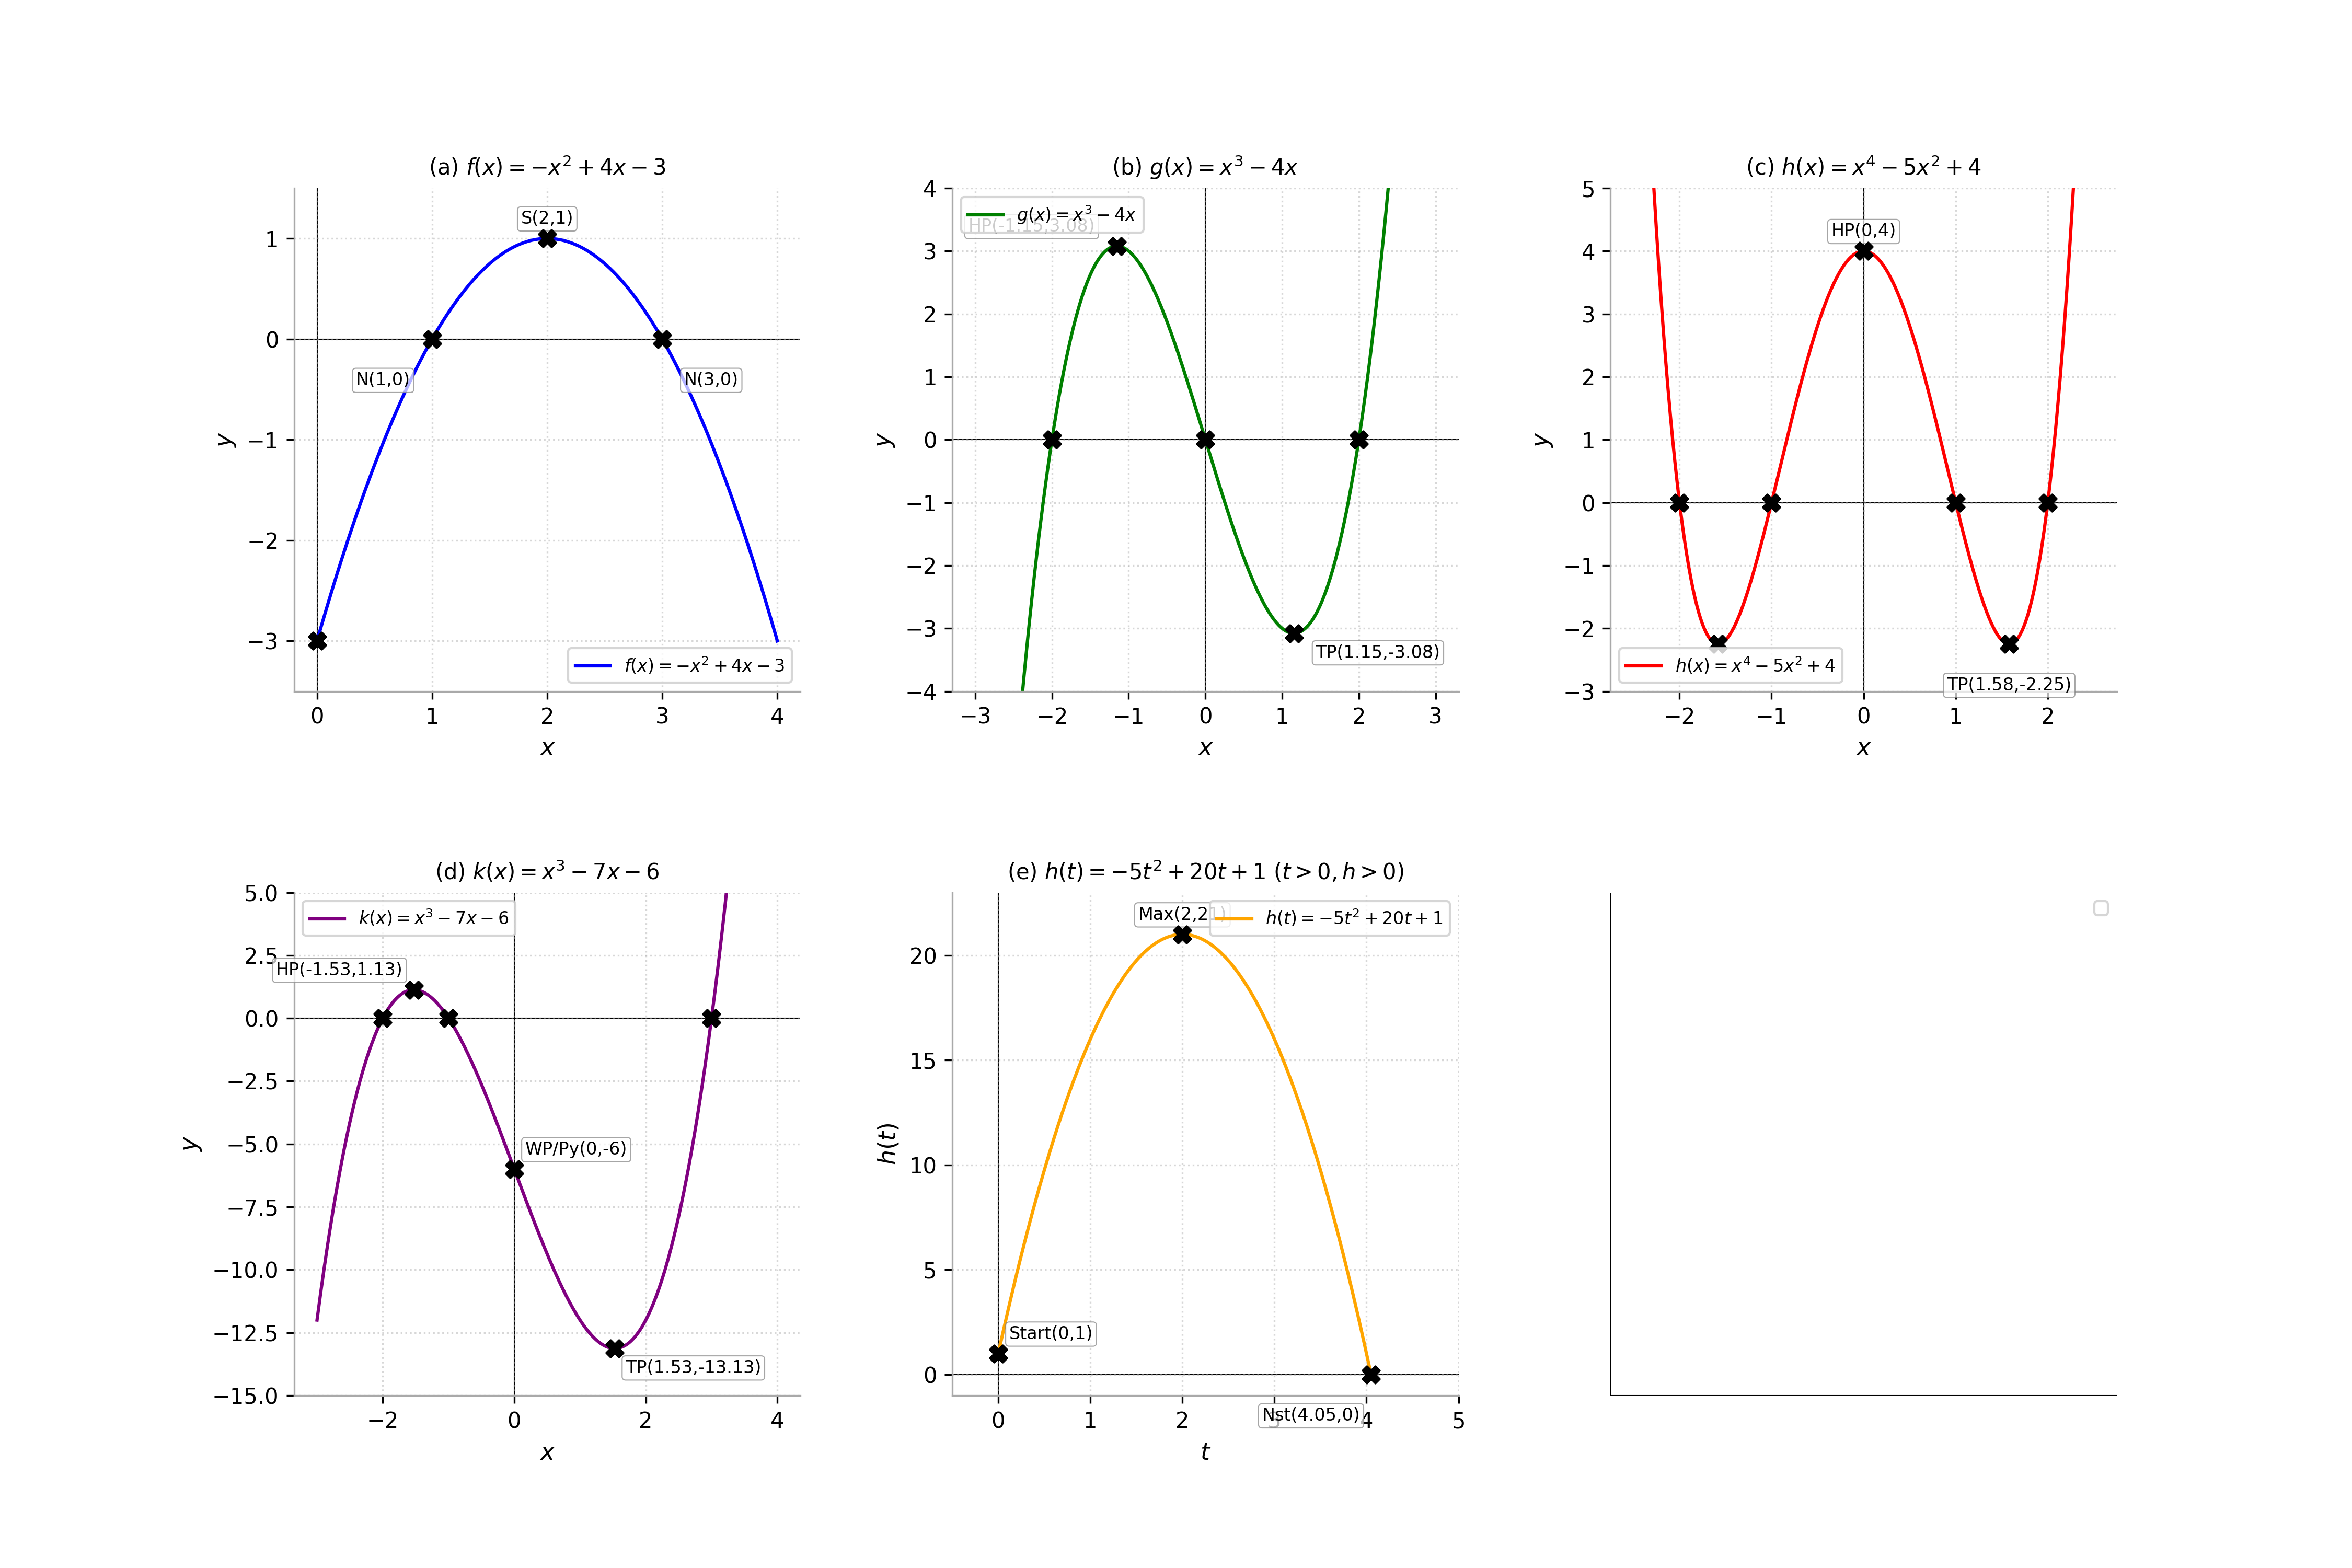
\includegraphics[width=0.8\textwidth]{grafiken/kurvendiskussionen_alle_graphen.png}
    \captionof{figure}{Graphen der untersuchten Funktionen: (a) $f(x)$, (b) $g(x)$, (c) $h(x)$, (d) $k(x)$, und (e) $h(t)$.}
    \label{fig:kurvendisk_alle_graphen}
\end{center}
\end{loesungsumgebung}



\begin{aufgabenumgebung}{Nullstellen aus faktorisierter Form bestimmen}
Bestimme die Nullstellen der folgenden Funktionen. Gib auch an, ob es sich um einfache oder mehrfache Nullstellen handelt. Eine Kurvendiskussion zu diesen Funktionen kann natürlich auch nie schaden.
\begin{enumerate}
    \item $f(x) = (x+4)(x-2.5)(x+1)$
    \item $g(x) = -3x^2(x-1)(x+2)^3$
    \item $h(x) = (x^2-9)(x+1)$ (Tipp: $x^2-9$ weiter faktorisieren!)
    \item $k(x) = 2x^4 - 8x^2$ (Tipp: Erst ausklammern, dann weiter überlegen.)
\end{enumerate}
\end{aufgabenumgebung}

\begin{loesungsumgebung}[loes:nullstellen-faktorisierte-form-wiederholung]{Nullstellen aus faktorisierter Form bestimmen}
Wir bestimmen die Nullstellen der gegebenen Funktionen, indem wir jeden Faktor gleich Null setzen (Satz vom Nullprodukt) und die Vielfachheit der Nullstelle anhand des Exponenten des jeweiligen Linearfaktors bestimmen.

\begin{enumerate}[label=(\alph*)]
    \item \textbf{Funktion $f(x) = (x+4)(x-2.5)(x+1)$} \\
    Setze $f(x)=0$: $(x+4)(x-2.5)(x+1) = 0$.
    \begin{itemize}
        \item $x+4 = 0 \Rightarrow x_1 = -4$. Dies ist eine \textbf{einfache} Nullstelle (Exponent 1).
        \item $x-2.5 = 0 \Rightarrow x_2 = 2.5$. Dies ist eine \textbf{einfache} Nullstelle (Exponent 1).
        \item $x+1 = 0 \Rightarrow x_3 = -1$. Dies ist eine \textbf{einfache} Nullstelle (Exponent 1).
    \end{itemize}
    Die Nullstellen sind $\mathbf{-4}$ (einfach), $\mathbf{2.5}$ (einfach) und $\mathbf{-1}$ (einfach).

    \item \textbf{Funktion $g(x) = -3x^2(x-1)(x+2)^3$} \\
    Setze $g(x)=0$: $-3x^2(x-1)(x+2)^3 = 0$.
    \begin{itemize}
        \item $-3x^2 = 0 \Rightarrow x^2 = 0 \Rightarrow x_1 = 0$. Da der Faktor $x$ mit dem Exponenten 2 auftritt ($x^2$), ist dies eine \textbf{doppelte} Nullstelle.
        \item $x-1 = 0 \Rightarrow x_2 = 1$. Dies ist eine \textbf{einfache} Nullstelle (Exponent 1).
        \item $(x+2)^3 = 0 \Rightarrow x+2 = 0 \Rightarrow x_3 = -2$. Da der Faktor $(x+2)$ mit dem Exponenten 3 auftritt, ist dies eine \textbf{dreifache} Nullstelle.
    \end{itemize}
    Die Nullstellen sind $\mathbf{0}$ (doppelt), $\mathbf{1}$ (einfach) und $\mathbf{-2}$ (dreifach).

    \item \textbf{Funktion $h(x) = (x^2-9)(x+1)$} \\
    Tipp: $x^2-9$ weiter faktorisieren. Mit der 3. binomischen Formel ist $x^2-9 = (x-3)(x+3)$.
    Somit ist $h(x) = (x-3)(x+3)(x+1)$.
    Setze $h(x)=0$: $(x-3)(x+3)(x+1) = 0$.
    \begin{itemize}
        \item $x-3 = 0 \Rightarrow x_1 = 3$. Dies ist eine \textbf{einfache} Nullstelle.
        \item $x+3 = 0 \Rightarrow x_2 = -3$. Dies ist eine \textbf{einfache} Nullstelle.
        \item $x+1 = 0 \Rightarrow x_3 = -1$. Dies ist eine \textbf{einfache} Nullstelle.
    \end{itemize}
    Die Nullstellen sind $\mathbf{3}$ (einfach), $\mathbf{-3}$ (einfach) und $\mathbf{-1}$ (einfach).

    \item \textbf{Funktion $k(x) = 2x^4 - 8x^2$} \\
    Tipp: Erst ausklammern.
    $k(x) = 2x^2(x^2-4)$.
    Den Term $x^2-4$ können wir weiter faktorisieren: $x^2-4 = (x-2)(x+2)$.
    Somit ist $k(x) = 2x^2(x-2)(x+2)$.
    Setze $k(x)=0$: $2x^2(x-2)(x+2) = 0$.
    \begin{itemize}
        \item $2x^2 = 0 \Rightarrow x^2=0 \Rightarrow x_1 = 0$. Dies ist eine \textbf{doppelte} Nullstelle (wegen $x^2$).
        \item $x-2 = 0 \Rightarrow x_2 = 2$. Dies ist eine \textbf{einfache} Nullstelle.
        \item $x+2 = 0 \Rightarrow x_3 = -2$. Dies ist eine \textbf{einfache} Nullstelle.
    \end{itemize}
    Die Nullstellen sind $\mathbf{0}$ (doppelt), $\mathbf{2}$ (einfach) und $\mathbf{-2}$ (einfach).
\end{enumerate}
Eine vollständige Kurvendiskussion würde zusätzlich Symmetrie, Verhalten im Unendlichen, Extrempunkte, Wendepunkte und das Krümmungsverhalten untersuchen. Die Kenntnis der Nullstellen und ihrer Vielfachheit ist dabei ein wichtiger erster Schritt, da sie Aufschluss über das Verhalten des Graphen an der x-Achse gibt (Schneiden bei einfacher/ungerader Vielfachheit, Berühren bei doppelter/gerader Vielfachheit).
\end{loesungsumgebung}



\begin{aufgabenumgebung}{Grenzwerte und Symmetrie gebrochen-rationaler Grundfunktionen}
\begin{enumerate}
    \item Bestimme den Definitionsbereich und das Verhalten für $x \to 0^+$ und $x \to 0^-$ für die folgenden Funktionen. Gib auch an, ob es sich um eine Polstelle mit oder ohne Vorzeichenwechsel handelt.
        \begin{itemize}
            \item $f_1(x) = \frac{3}{x^3}$
            \item $f_2(x) = -\frac{1}{x^4}$
            \item $f_3(x) = \frac{10}{x}$
        \end{itemize}
    \item Untersuche die Symmetrie der Funktionen aus Teilaufgabe 1 (Achsensymmetrie zur y-Achse oder Punktsymmetrie zum Ursprung).
    \item \textbf{Zuordnung Aufgabe:} Ordne den folgenden Funktionsgraphen $k_1(x) = \frac{1}{x^2}$, $k_2(x) = -\frac{1}{x}$, $k_3(x) = \frac{2}{x^3}$, $k_4(x) = \frac{1}{x^4}$ die passenden Funktionsgleichungen zu. Begründe deine Entscheidung anhand des Verhaltens an der Polstelle $x=0$ und der Symmetrie.
    \begin{center}
        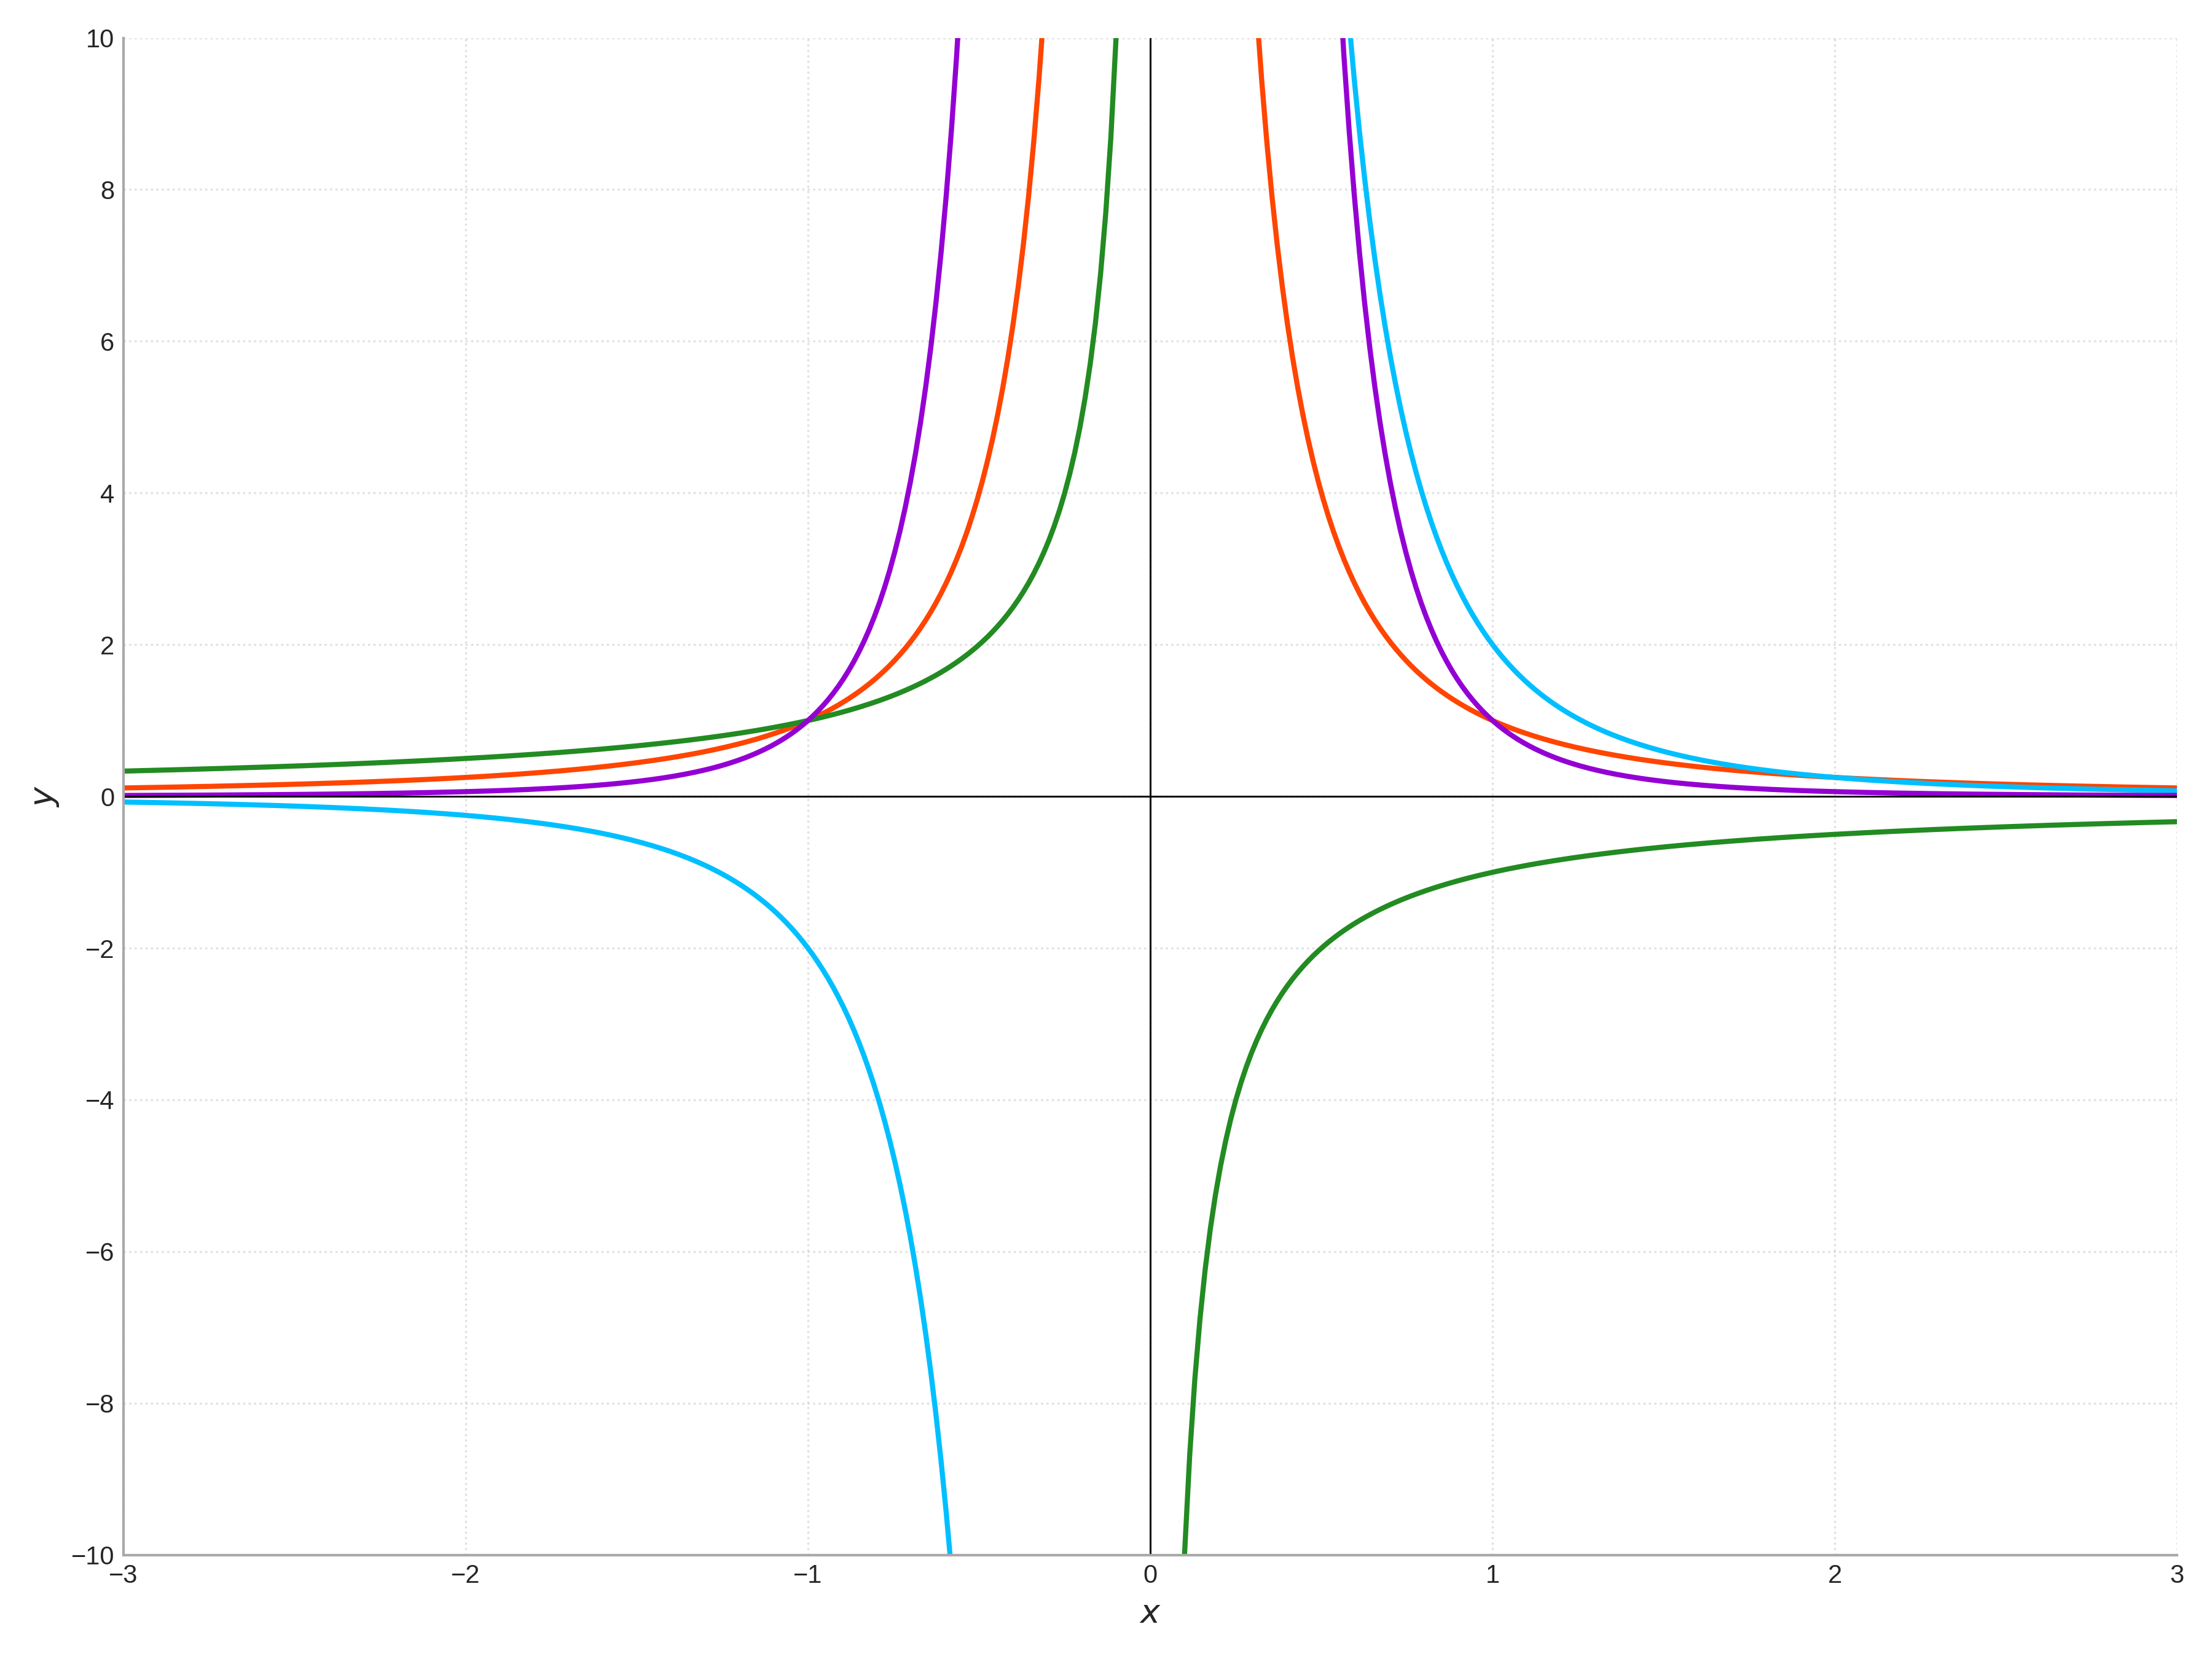
\includegraphics[width=0.9\textwidth]{grafiken/Zuordnung_Polstellen.png}
        \captionof{figure}{Graphen zur Zuordnung von Polstellenverhalten}
        \label{fig:zuordnung_polstellen}
    \end{center}
\end{enumerate}
\end{aufgabenumgebung}

\begin{loesungsumgebung}[loes:grenzwerte-symmetrie-gebrochen-rational]{Grenzwerte und Symmetrie gebrochen-rationaler Grundfunktionen}

\begin{enumerate}[label=(\alph*)]
    \item \textbf{Definitionsbereich und Verhalten für $x \to 0^\pm$}
    \begin{itemize}
        \item \textbf{Funktion $f_1(x) = \frac{3}{x^3}$}
        \begin{itemize}
            \item Definitionsbereich: $D_{f1} = \mathbb{R} \setminus \{0\}$.
            \item Verhalten an der Polstelle $x=0$:
            Für $x \to 0^+$: $x^3 \to 0^+$ (kleine positive Werte) $\implies f_1(x) = \frac{3}{x^3} \to +\infty$.
            Für $x \to 0^-$: $x^3 \to 0^-$ (kleine negative Werte) $\implies f_1(x) = \frac{3}{x^3} \to -\infty$.
            \item Es handelt sich um eine \textbf{Polstelle mit Vorzeichenwechsel} (VZW), da der Exponent im Nenner (3) ungerade ist.
        \end{itemize}

        \item \textbf{Funktion $f_2(x) = -\frac{1}{x^4}$}
        \begin{itemize}
            \item Definitionsbereich: $D_{f2} = \mathbb{R} \setminus \{0\}$.
            \item Verhalten an der Polstelle $x=0$:
            Für $x \to 0^+$: $x^4 \to 0^+$ $\implies f_2(x) = -\frac{1}{x^4} \to -\infty$.
            Für $x \to 0^-$: $x^4 \to 0^+$ $\implies f_2(x) = -\frac{1}{x^4} \to -\infty$.
            \item Es handelt sich um eine \textbf{Polstelle ohne Vorzeichenwechsel} (OVZW), da der Exponent im Nenner (4) gerade ist. Beide Äste gehen gegen $-\infty$.
        \end{itemize}

        \item \textbf{Funktion $f_3(x) = \frac{10}{x}$}
        \begin{itemize}
            \item Definitionsbereich: $D_{f3} = \mathbb{R} \setminus \{0\}$.
            \item Verhalten an der Polstelle $x=0$:
            Für $x \to 0^+$: $x \to 0^+$ $\implies f_3(x) = \frac{10}{x} \to +\infty$.
            Für $x \to 0^-$: $x \to 0^-$ $\implies f_3(x) = \frac{10}{x} \to -\infty$.
            \item Es handelt sich um eine \textbf{Polstelle mit Vorzeichenwechsel} (VZW), da der Exponent im Nenner (1) ungerade ist.
        \end{itemize}
    \end{itemize}

    \item \textbf{Symmetrieuntersuchung der Funktionen aus Teilaufgabe 1}
    \begin{itemize}
        \item \textbf{Funktion $f_1(x) = \frac{3}{x^3}$}
        $f_1(-x) = \frac{3}{(-x)^3} = \frac{3}{-x^3} = -\frac{3}{x^3} = -f_1(x)$.
        Die Funktion $f_1(x)$ ist \textbf{punktsymmetrisch zum Ursprung}.

        \item \textbf{Funktion $f_2(x) = -\frac{1}{x^4}$}
        $f_2(-x) = -\frac{1}{(-x)^4} = -\frac{1}{x^4} = f_2(x)$.
        Die Funktion $f_2(x)$ ist \textbf{achsensymmetrisch zur y-Achse}.

        \item \textbf{Funktion $f_3(x) = \frac{10}{x}$}
        $f_3(-x) = \frac{10}{(-x)} = -\frac{10}{x} = -f_3(x)$.
        Die Funktion $f_3(x)$ ist \textbf{punktsymmetrisch zum Ursprung}.
    \end{itemize}

    \item \textbf{Zuordnung Aufgabe:}
    Wir analysieren die gegebenen Funktionen $k_1(x) = \frac{1}{x^2}$, $k_2(x) = -\frac{1}{x}$, $k_3(x) = \frac{2}{x^3}$, $k_4(x) = \frac{1}{x^4}$ und ordnen sie den Graphen in der Abbildung zu (die Farben beziehen sich auf die typische Darstellung solcher Graphen in der von Ihnen hochgeladenen Abbildung).

    \begin{itemize}
        \item \textbf{$k_1(x) = \frac{1}{x^2}$:}
        \begin{itemize}
            \item Verhalten bei $x=0$: Polstelle ohne Vorzeichenwechsel. $\lim_{x \to 0^\pm} k_1(x) = +\infty$. (Beide Äste gehen nach oben).
            \item Symmetrie: $k_1(-x) = \frac{1}{(-x)^2} = \frac{1}{x^2} = k_1(x) \implies$ Achsensymmetrisch zur y-Achse.
            \item Werte: $k_1(x) > 0$ für alle $x \neq 0$. $k_1(1)=1, k_1(2)=0.25$.
        \end{itemize}
        \textit{Mathematische Begründung für Zuordnung:} Dieser Graph muss achsensymmetrisch sein und sich für $x \to 0$ nach $+\infty$ entwickeln.
        In der typischen Darstellung (Abbildung 5.10) ist dies der \textbf{orange Graph}. Er ist achsensymmetrisch und beide Äste streben gegen $+\infty$.

        \item \textbf{$k_2(x) = -\frac{1}{x}$:}
        \begin{itemize}
            \item Verhalten bei $x=0$: Polstelle mit Vorzeichenwechsel. $\lim_{x \to 0^+} k_2(x) = -\infty$, $\lim_{x \to 0^-} k_2(x) = +\infty$.
            \item Symmetrie: $k_2(-x) = -\frac{1}{-x} = \frac{1}{x} = -(-\frac{1}{x}) = -k_2(x) \implies$ Punktsymmetrisch zum Ursprung.
            \item Werte: Für $x>0$ ist $k_2(x)<0$ (IV. Quadrant). Für $x<0$ ist $k_2(x)>0$ (II. Quadrant).
        \end{itemize}
        \textit{Mathematische Begründung für Zuordnung:} Dieser Graph muss punktsymmetrisch sein, wobei der rechte Ast ($x>0$) nach $-\infty$ und der linke Ast ($x<0$) nach $+\infty$ strebt.
        In der typischen Darstellung (Abbildung 5.10) ist dies der \textbf{hellblaue (cyan) Graph}.

        \item \textbf{$k_3(x) = \frac{2}{x^3}$:}
        \begin{itemize}
            \item Verhalten bei $x=0$: Polstelle mit Vorzeichenwechsel. $\lim_{x \to 0^+} k_3(x) = +\infty$, $\lim_{x \to 0^-} k_3(x) = -\infty$.
            \item Symmetrie: $k_3(-x) = \frac{2}{(-x)^3} = -\frac{2}{x^3} = -k_3(x) \implies$ Punktsymmetrisch zum Ursprung.
            \item Werte: Für $x>0$ ist $k_3(x)>0$ (I. Quadrant). Für $x<0$ ist $k_3(x)<0$ (III. Quadrant). Der Faktor 2 im Zähler bewirkt eine Streckung im Vergleich zu $1/x^3$.
        \end{itemize}
        \textit{Mathematische Begründung für Zuordnung:} Dieser Graph muss punktsymmetrisch sein, wobei der rechte Ast ($x>0$) nach $+\infty$ und der linke Ast ($x<0$) nach $-\infty$ strebt.
        In der typischen Darstellung (Abbildung 5.10) ist dies der \textbf{grüne Graph}.

        \item \textbf{$k_4(x) = \frac{1}{x^4}$:}
        \begin{itemize}
            \item Verhalten bei $x=0$: Polstelle ohne Vorzeichenwechsel. $\lim_{x \to 0^\pm} k_4(x) = +\infty$. (Beide Äste gehen nach oben).
            \item Symmetrie: $k_4(-x) = \frac{1}{(-x)^4} = \frac{1}{x^4} = k_4(x) \implies$ Achsensymmetrisch zur y-Achse.
            \item Werte: $k_4(x) > 0$ für alle $x \neq 0$. Im Vergleich zu $k_1(x)=1/x^2$: Für $|x|<1$ ist $x^4 < x^2 \implies 1/x^4 > 1/x^2$ (steilerer Anstieg gegen Pol). Für $|x|>1$ ist $x^4 > x^2 \implies 1/x^4 < 1/x^2$ (schnellere Annäherung an die x-Achse).
        \end{itemize}
        \textit{Mathematische Begründung für Zuordnung:} Dieser Graph muss achsensymmetrisch sein, sich für $x \to 0$ nach $+\infty$ entwickeln und im Vergleich zu $1/x^2$ steiler an der Polstelle sein und sich schneller der x-Achse annähern.
        In der typischen Darstellung (Abbildung 5.10) ist dies der \textbf{lila (purple) Graph}. Er ist achsensymmetrisch, beide Äste streben gegen $+\infty$ und er ist 'enger' an der y-Achse und flacher für größere $|x|$ im Vergleich zum orangen Graphen.
    \end{itemize}
    \textbf{Zusammenfassende Zuordnung (basierend auf typischer Farbgebung der Abbildung 5.10):}
    \begin{itemize}
        \item Orange Kurve: $k_1(x) = \frac{1}{x^2}$
        \item Hellblaue (Cyan) Kurve: $k_2(x) = -\frac{1}{x}$
        \item Grüne Kurve: $k_3(x) = \frac{2}{x^3}$
        \item Lila (Purple) Kurve: $k_4(x) = \frac{1}{x^4}$
    \end{itemize}
\end{enumerate}

\end{loesungsumgebung}


\begin{aufgabenumgebung}{Funktionen mit negativen Exponenten und Substitution}
\begin{enumerate}
    \item Bestimme für die folgenden Funktionen den Definitionsbereich, die Gleichung der senkrechten Asymptote(n) und das Verhalten der Funktion für $x$ gegen die Polstelle(n) (einseitige Grenzwerte) sowie für $x \to \pm\infty$. Untersuche auch das Symmetrieverhalten bezüglich der senkrechten Asymptote oder eines Punktes.
        \begin{itemize}
            \item $f_1(x) = \frac{-1}{x+2}$
            \item $f_2(x) = \frac{3}{(x-3)^2}$
            \item $f_3(x) = 1 - \frac{1}{x^2}$ (Tipp: Was ist hier die horizontale Asymptote?)
        \end{itemize}
    \item Skizziere die Graphen der Funktionen aus Teilaufgabe 1.
    \item \textbf{Transformationskette verstehen:}
        Beschreibe, wie der Graph der Funktion $g(x) = \frac{-2}{(x+3)^2} - 4$ aus dem Graphen der Grundfunktion $h(u) = \frac{1}{u^2}$ durch Streckung/Stauchung, Spiegelung und Verschiebungen hervorgeht. Gib den Definitionsbereich und die Gleichungen der Asymptoten von $g(x)$ an.
\end{enumerate}
\end{aufgabenumgebung}

\begin{loesungsumgebung}[loes:funktionen-neg-exponent-substitution]{Funktionen mit negativen Exponenten und Substitution}

\begin{enumerate}[label=(\alph*)]
    \item \textbf{Untersuchung der Funktionen $f_1(x), f_2(x), f_3(x)$}
    \begin{itemize}
        \item \textbf{Funktion $f_1(x) = \frac{-1}{x+2}$}
        \begin{itemize}
            \item \textit{Definitionsbereich:} Der Nenner $x+2$ darf nicht Null sein, also $x \neq -2$. $D_{f1} = \mathbb{R} \setminus \{-2\}$.
            \item \textit{Senkrechte Asymptote:} Bei $x=-2$ liegt eine Polstelle vor. Die Gleichung der senkrechten Asymptote ist $\mathbf{x=-2}$.
            \item \textit{Verhalten an der Polstelle $x=-2$:}
            Für $x \to -2^+$ (z.B. $x=-1.9$, $x+2$ ist klein und positiv): $f_1(x) = \frac{-1}{\text{klein pos.}} \to -\infty$.
            Für $x \to -2^-$ (z.B. $x=-2.1$, $x+2$ ist klein und negativ): $f_1(x) = \frac{-1}{\text{klein neg.}} \to +\infty$.
            Es handelt sich um eine Polstelle mit Vorzeichenwechsel.
            \item \textit{Verhalten für $x \to \pm\infty$:}
            $\lim_{x \to \pm\infty} \frac{-1}{x+2} = \lim_{x \to \pm\infty} \frac{-1/x}{1+2/x} = \frac{0}{1} = 0$.
            Die horizontale Asymptote ist $\mathbf{y=0}$.
            \item \textit{Symmetrie:} Der Graph von $f_1(x)$ ist punktsymmetrisch zum Schnittpunkt seiner Asymptoten, dem Punkt $\mathbf{(-2|0)}$. (Verschobene Hyperbel $y' = -1/x'$ um $(-2,0)$).
        \end{itemize}

        \item \textbf{Funktion $f_2(x) = \frac{3}{(x-3)^2}$}
        \begin{itemize}
            \item \textit{Definitionsbereich:} Der Nenner $(x-3)^2$ darf nicht Null sein, also $x \neq 3$. $D_{f2} = \mathbb{R} \setminus \{3\}$.
            \item \textit{Senkrechte Asymptote:} Bei $x=3$ liegt eine Polstelle vor. Die Gleichung der senkrechten Asymptote ist $\mathbf{x=3}$.
            \item \textit{Verhalten an der Polstelle $x=3$:}
            Der Nenner $(x-3)^2$ ist für $x \neq 3$ immer positiv und geht gegen $0^+$ für $x \to 3^\pm$.
            Für $x \to 3^+$: $f_2(x) = \frac{3}{(x-3)^2} \to \frac{3}{\text{klein pos.}} \to +\infty$.
            Für $x \to 3^-$: $f_2(x) = \frac{3}{(x-3)^2} \to \frac{3}{\text{klein pos.}} \to +\infty$.
            Es handelt sich um eine Polstelle ohne Vorzeichenwechsel.
            \item \textit{Verhalten für $x \to \pm\infty$:}
            $\lim_{x \to \pm\infty} \frac{3}{(x-3)^2} = 0$.
            Die horizontale Asymptote ist $\mathbf{y=0}$.
            \item \textit{Symmetrie:} Der Graph von $f_2(x)$ ist achsensymmetrisch zur senkrechten Asymptote $\mathbf{x=3}$. (Verschobene und gestreckte Funktion $y' = 1/(x')^2$).
        \end{itemize}

        \item \textbf{Funktion $f_3(x) = 1 - \frac{1}{x^2}$}
        \begin{itemize}
            \item \textit{Definitionsbereich:} Der Nenner $x^2$ darf nicht Null sein, also $x \neq 0$. $D_{f3} = \mathbb{R} \setminus \{0\}$.
            \item \textit{Senkrechte Asymptote:} Bei $x=0$ liegt eine Polstelle vor. Die Gleichung der senkrechten Asymptote ist $\mathbf{x=0}$ (die y-Achse).
            \item \textit{Verhalten an der Polstelle $x=0$:}
            Der Term $x^2$ ist für $x \neq 0$ immer positiv und geht gegen $0^+$ für $x \to 0^\pm$.
            Somit $\frac{1}{x^2} \to +\infty$ für $x \to 0^\pm$.
            Daher $f_3(x) = 1 - \frac{1}{x^2} \to 1 - (+\infty) \to -\infty$ für $x \to 0^\pm$.
            Es handelt sich um eine Polstelle ohne Vorzeichenwechsel (für den gebrochen-rationalen Anteil, beide Äste von $f_3(x)$ gehen gegen $-\infty$).
            \item \textit{Verhalten für $x \to \pm\infty$:}
            $\lim_{x \to \pm\infty} \frac{1}{x^2} = 0$.
            $\lim_{x \to \pm\infty} \left(1 - \frac{1}{x^2}\right) = 1 - 0 = 1$.
            Die horizontale Asymptote ist $\mathbf{y=1}$.
            \item \textit{Symmetrie:} $f_3(-x) = 1 - \frac{1}{(-x)^2} = 1 - \frac{1}{x^2} = f_3(x)$.
            Der Graph von $f_3(x)$ ist \textbf{achsensymmetrisch zur y-Achse} (welche die senkrechte Asymptote ist).
        \end{itemize}
    \end{itemize}

    \item \textbf{Skizze der Graphen aus Teilaufgabe 1} \\
    Die Graphen werden in einem gemeinsamen Koordinatensystem skizziert, wobei die jeweiligen Asymptoten und das Verhalten an den Polstellen sowie im Unendlichen berücksichtigt werden.
    \begin{center}
    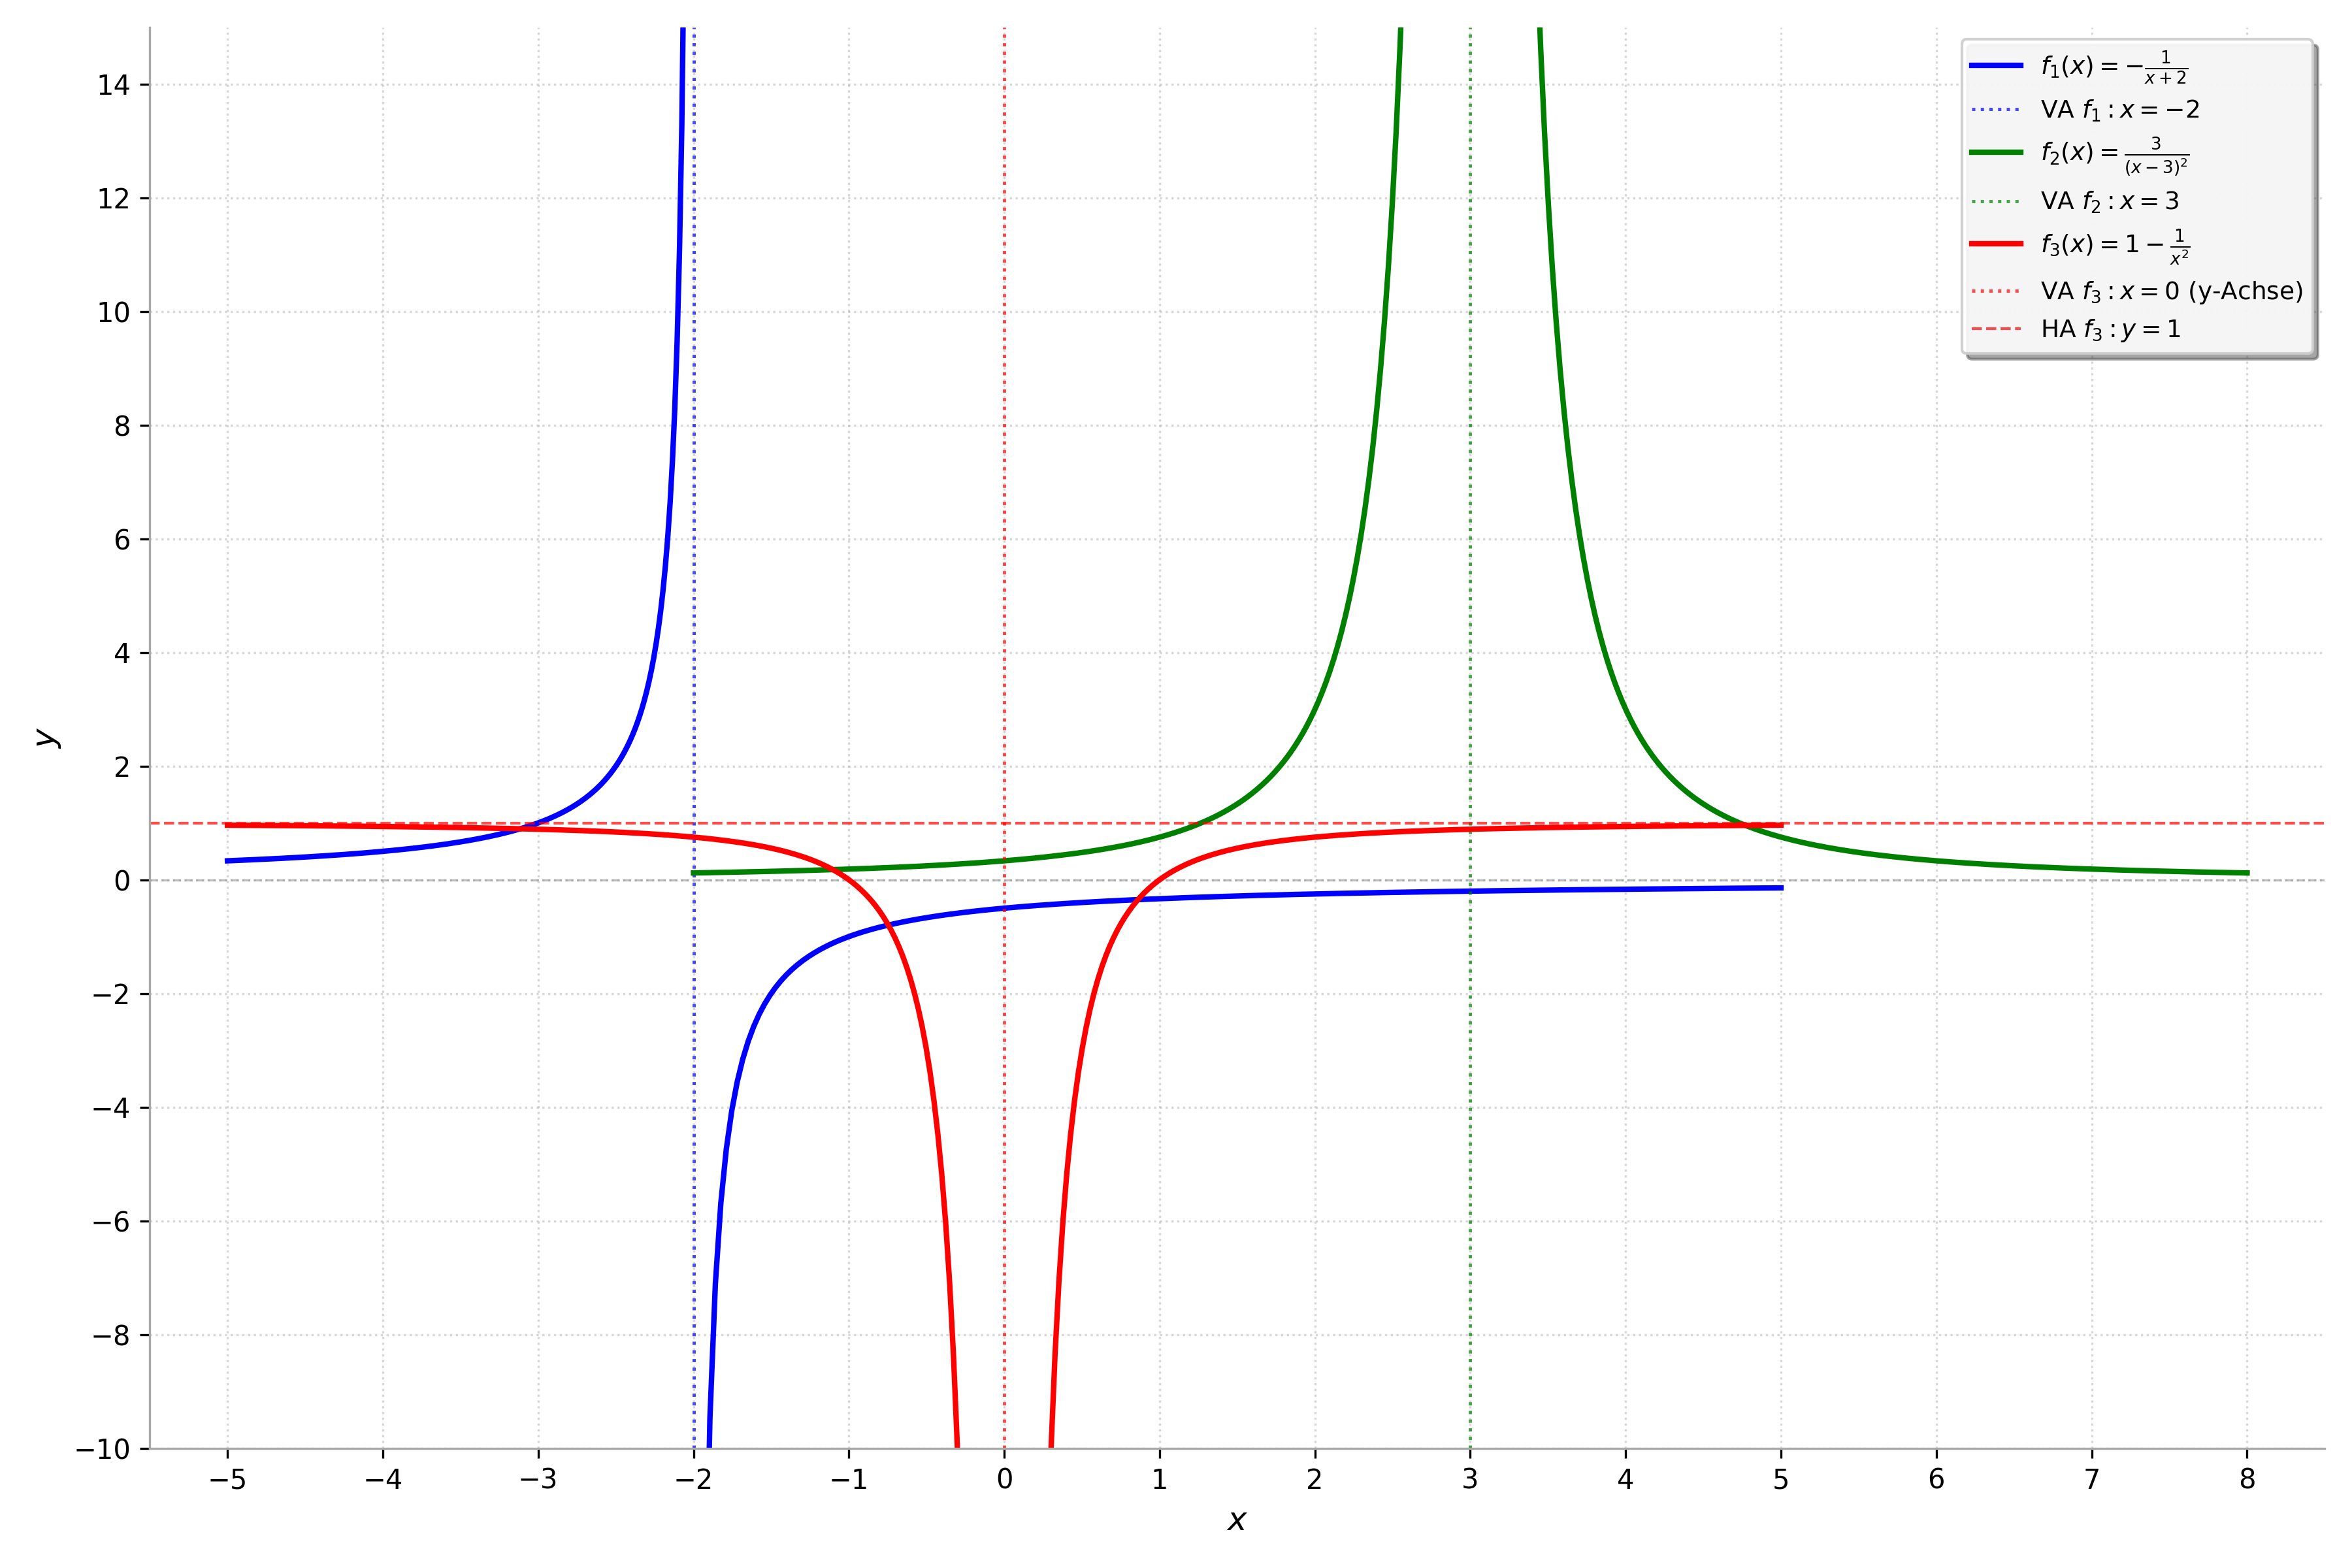
\includegraphics[width=0.8\textwidth]{grafiken/funktionen_neg_exp_kombi_graph.png}
    % --- Beschreibung der Grafik ---
    % Die Grafik zeigt ein Koordinatensystem mit drei Graphen:
    % 1. f1(x) = -1/(x+2): VA bei x=-2, HA bei y=0. Hyperbelähnliche Äste im II. und IV. Quadranten relativ zum Asymptotenkreuz (-2|0). Für x -> -2+ geht f1 -> -unendlich, für x -> -2- geht f1 -> +unendlich.
    % 2. f2(x) = 3/((x-3)^2): VA bei x=3, HA bei y=0. Beide Äste gehen für x -> 3 gegen +unendlich. Symmetrisch zu x=3.
    % 3. f3(x) = 1 - 1/x^2: VA bei x=0 (y-Achse), HA bei y=1. Beide Äste gehen für x -> 0 gegen -unendlich. Symmetrisch zur y-Achse. Der Graph nähert sich von unten der Asymptote y=1.
    \captionof{figure}{Skizzen der Graphen von $f_1(x)$, $f_2(x)$ und $f_3(x)$ mit ihren Asymptoten.}
    \label{fig:funktionen_neg_exp_kombi_graph}
    \end{center}

    \item \textbf{Transformationskette verstehen: $g(x) = \frac{-2}{(x+3)^2} - 4$ aus $h(u) = \frac{1}{u^2}$}
    Der Graph von $g(x)$ geht aus dem Graphen der Grundfunktion $h(u) = \frac{1}{u^2}$ durch folgende Transformationen hervor:
    \begin{enumerate}
        \item \textbf{Streckung in y-Richtung} mit dem Faktor 2: $h_1(u) = 2 \cdot h(u) = \frac{2}{u^2}$.
        \item \textbf{Spiegelung an der x-Achse:} $h_2(u) = -h_1(u) = -\frac{2}{u^2}$.
        \item \textbf{Verschiebung um 3 Einheiten nach links} in x-Richtung (ersetze $u$ durch $x+3$): $h_3(x) = h_2(x+3) = -\frac{2}{(x+3)^2}$.
        \item \textbf{Verschiebung um 4 Einheiten nach unten} in y-Richtung: $g(x) = h_3(x) - 4 = -\frac{2}{(x+3)^2} - 4$.
    \end{enumerate}
    \textbf{Definitionsbereich von $g(x)$:}
    Der Nenner $(x+3)^2$ darf nicht Null sein, also $x+3 \neq 0 \Rightarrow x \neq -3$.
    $D_g = \mathbb{R} \setminus \{-3\}$.
    \textbf{Gleichungen der Asymptoten von $g(x)$:}
    \begin{itemize}
        \item Die Verschiebung nach links ändert die senkrechte Asymptote von $u=0$ zu $x+3=0$, also $\mathbf{x=-3}$.
        \item Die Streckung und Spiegelung beeinflussen die horizontale Asymptote $y=0$ nicht. Die Verschiebung nach unten um 4 Einheiten verschiebt die horizontale Asymptote zu $\mathbf{y=-4}$.
        ($\lim_{x \to \pm\infty} \left(-\frac{2}{(x+3)^2} - 4\right) = 0 - 4 = -4$).
    \end{itemize}
\end{enumerate}

\end{loesungsumgebung}


\begin{aufgabenumgebung}[A:DiffUebergreifend]{Übergreifende Übungsaufgaben zum bisherigen Kapitel Differentialrechnung}
\begin{enumerate}
    \item \textbf{Polynom-Analyse (Grad 3):}
        Gegeben ist die Funktion $f(x) = -\frac{1}{3}x^3 + x^2 + 3x - \frac{7}{3}$.
        \begin{enumerate}
            \item Führe eine vollständige Kurvendiskussion für $f(x)$ durch (Definitionsbereich, Symmetrie, Verhalten im Unendlichen, Achsenschnittpunkte, Extrempunkte, Wendepunkte, Monotonie, Krümmung).
            \item Zeichne den Graphen von $f(x)$ im Intervall $[-4, 6]$ unter Verwendung deiner Ergebnisse.
            \item Bestimme die Gleichung der Tangente an den Graphen von $f(x)$ im Punkt $P(0|f(0))$.
            \item In welchem Punkt hat die Tangente an den Graphen von $f(x)$ die Steigung $m=-5$?
        \end{enumerate}
    \item \textbf{Optimierungsproblem – Die optimale Dose:}
        Eine zylinderförmige Konservendose soll ein Volumen von $V = 500 \text{ cm}^3$ haben. Die Materialkosten sollen minimiert werden, d.h. die Oberfläche $O$ der Dose soll minimal werden.
        Die Formeln für einen Zylinder mit Radius $r$ und Höhe $h$ sind:
        Volumen: $V = \pi r^2 h$
        Oberfläche (Mantel + 2 Deckel): $O = 2\pi r^2 + 2\pi r h$
        \begin{enumerate}
            \item \textbf{Zielfunktion aufstellen:} Drücke die Oberfläche $O$ als Funktion nur einer Variablen (z.B. des Radius $r$) aus. Nutze dazu die Nebenbedingung für das Volumen $V=500 \text{ cm}^3$, um $h$ durch $r$ auszudrücken und in die Oberflächenformel einzusetzen. Du erhältst $O(r)$.
            \item \textbf{Ableitung bilden:} Bilde die erste Ableitung $O'(r)$. (Hinweis: $O(r)$ wird einen Term der Form $\frac{k}{r}$ enthalten, was du als $kr^{-1}$ schreiben kannst.)
            \item \textbf{Extremstelle finden:} Setze $O'(r)=0$ und löse nach $r$ auf, um den Radius zu finden, der die Oberfläche minimiert.
            \item \textbf{Überprüfung (optional für Experten):} Überprüfe mit der zweiten Ableitung $O''(r)$, ob es sich tatsächlich um ein Minimum handelt.
            \item \textbf{Optimale Abmessungen:} Berechne die zugehörige Höhe $h$ und das minimale Oberflächenmaterial. Welcher Zusammenhang besteht zwischen $r$ und $h$ bei minimaler Oberfläche?
        \end{enumerate}
    \item \textbf{Analyse einer biquadratischen Funktion:}
        Gegeben ist die Funktion $f(x) = x^4 - 8x^2 + 7$.
        \begin{enumerate}
            \item Untersuche die Funktion auf Symmetrie.
            \item Bestimme die Nullstellen der Funktion. (Tipp: Substitution $z=x^2$).
            \item Bestimme die lokalen Extrempunkte von $f(x)$.
            \item Bestimme die Wendepunkte von $f(x)$.
            \item Skizziere den Graphen von $f(x)$ basierend auf deinen Ergebnissen.
        \end{enumerate}
    \item \textbf{Transformationen und Grenzwerte verstehen:}
        Betrachte die Funktion $g(x) = \frac{-2}{(x+1)^3} + 1$.
        \begin{enumerate}
            \item \textbf{Grundfunktion:} Von welcher einfachen Grundfunktion $h(u) = \frac{a}{u^n}$ lässt sich $g(x)$ ableiten?
            \item \textbf{Transformationsschritte:} Beschreibe, durch welche Verschiebungen, Streckungen oder Spiegelungen der Graph von $g(x)$ aus dem Graphen von $h(u)$ entsteht.
            \item \textbf{Definitionsbereich und Asymptoten:} Bestimme den Definitionsbereich von $g(x)$ sowie die Gleichungen der senkrechten und waagerechten Asymptoten.
            \item \textbf{Grenzwerte an der Polstelle:} Untersuche $\lim_{x \to -1^+} g(x)$ und $\lim_{x \to -1^-} g(x)$. Handelt es sich um eine Polstelle mit oder ohne Vorzeichenwechsel?
            \item \textbf{Skizze:} Skizziere den Graphen von $g(x)$ mit seinen Asymptoten.
        \end{enumerate}
    \item \textbf{Bewegung eines Objekts (Anwendung):}
        Die Höhe $h$ (in Metern) eines senkrecht nach oben geworfenen Steins nach $t$ Sekunden wird durch die Funktion $h(t) = -5t^2 + 20t + 1$ beschrieben (für $t \ge 0$ und solange $h(t) \ge 0$).
        \begin{enumerate}
            \item Bestimme die Funktion $v(t)$, die die Geschwindigkeit des Autos zum Zeitpunkt $t$ angibt.
            \item Bestimme die Funktion $a(t)$, die die Beschleunigung des Autos zum Zeitpunkt $t$ angibt.
            \item Zu welchen Zeitpunkten $t$ ist das Auto in Ruhe (Geschwindigkeit gleich Null)?
            \item In welchen Zeitintervallen fährt das Auto vorwärts ($v(t)>0$) und in welchen rückwärts ($v(t)<0$)?
            \item Wann ist die Beschleunigung Null? Was bedeutet das für die Geschwindigkeit zu diesem Zeitpunkt?
            \item (Für Experten): Wann ist die Geschwindigkeit des Autos am größten im Intervall $[0, 2]$? Wann ist sie am geringsten (d.h. am stärksten negativ) im Intervall $[0, 4]$?
        \end{enumerate}
\end{enumerate}
\end{aufgabenumgebung}



\begin{loesungsumgebung}[loes:A:DiffUebergreifend-KombiGraph]{Übergreifende Übungsaufgaben}
Die Graphen zu den Kurvendiskussionen in Aufgabe 1, 3 und 4 finden Sie in Abbildung \ref{fig:uebergreifend_alle_graphen} am Ende dieser Lösung.

\begin{enumerate}
    \item \textbf{Polynom-Analyse (Grad 3): $f(x) = -\frac{1}{3}x^3 + x^2 + 3x - \frac{7}{3}$}
    \begin{enumerate}[label=(\alph*)]
        \item \textbf{Vollständige Kurvendiskussion:}
        \begin{enumerate}[label=\arabic*.]
            \item \textbf{Definitionsbereich ($D_f$):} $D_f = \mathbb{R}$.
            \item \textbf{Symmetrie:}
            $f(-x) = -\frac{1}{3}(-x)^3 + (-x)^2 + 3(-x) - \frac{7}{3} = \frac{1}{3}x^3 + x^2 - 3x - \frac{7}{3}$.
            Keine einfache Symmetrie zum Koordinatensystem erkennbar ($f(-x) \neq f(x)$ und $f(-x) \neq -f(x)$).
            \item \textbf{Verhalten im Unendlichen:} Leitterm ist $-\frac{1}{3}x^3$.
            $\lim_{x \to \infty} f(x) = -\infty$; $\lim_{x \to -\infty} f(x) = +\infty$. (Verlauf von links oben nach rechts unten).
            \item \textbf{Schnittpunkt mit der y-Achse ($P_y$):} $f(0) = -\frac{7}{3}$. $P_y(0|-\frac{7}{3})$.
            \item \textbf{Nullstellen ($N_i$):}
            Der Tipp gibt $x_1=1$ als Nullstelle an. Überprüfung: $f(1) = -\frac{1}{3}(1)^3 + (1)^2 + 3(1) - \frac{7}{3} = -\frac{1}{3} + 1 + 3 - \frac{7}{3} = 4 - \frac{8}{3} = \frac{4}{3} \neq 0$.
            Der Tipp ist somit für die gegebene Funktion $f(x)$ nicht korrekt. Die exakte algebraische Bestimmung der Nullstellen dieses Polynoms 3. Grades ist ohne eine leicht zu ratende Nullstelle aufwendig. Numerische Verfahren könnten verwendet werden, oder es liegt eine Abweichung in der Aufgabenstellung/Funktion vor. Für die qualitative Skizze konzentrieren wir uns auf die anderen Punkte.
            \item \textbf{Erste Ableitung $f'(x)$:} $f'(x) = -x^2 + 2x + 3$.
            \item \textbf{Extremstellen:} Notwendige Bedingung: $f'(x_E)=0 \Rightarrow -x^2 + 2x + 3 = 0 \Rightarrow x^2 - 2x - 3 = 0$.
            Lösung mit p-q-Formel oder Faktorisierung: $(x-3)(x+1)=0 \Rightarrow x_{E1}=3, x_{E2}=-1$.
            \item \textbf{Zweite Ableitung $f''(x)$:} $f''(x) = -2x + 2$.
            \item \textbf{Art der Extremstellen:}
            $f''(3) = -2(3)+2 = -4 < 0 \implies$ Hochpunkt bei $x_E=3$.
            $y_H = f(3) = -\frac{1}{3}(27) + 9 + 3(3) - \frac{7}{3} = -9+9+9-\frac{7}{3} = \frac{20}{3}$. Hochpunkt $\mathbf{H(3|20/3)}$.
            $f''(-1) = -2(-1)+2 = 4 > 0 \implies$ Tiefpunkt bei $x_E=-1$.
            $y_T = f(-1) = -\frac{1}{3}(-1) + 1 + 3(-1) - \frac{7}{3} = \frac{1}{3} - 2 - \frac{7}{3} = -2 - \frac{6}{3} = -4$. Tiefpunkt $\mathbf{T(-1|-4)}$.
            \item \textbf{Monotonie:} $f'(x) = -(x-3)(x+1)$. Die Parabel $f'(x)$ ist nach unten geöffnet.
            $f'(x) < 0$ für $x < -1$ und $x > 3 \implies f$ ist streng monoton fallend.
            $f'(x) > 0$ für $-1 < x < 3 \implies f$ ist streng monoton steigend.
            \item \textbf{Wendepunkte:} Notwendige Bedingung: $f''(x_W)=0 \Rightarrow -2x_W+2=0 \Rightarrow x_W=1$.
            Dritte Ableitung: $f'''(x)=-2$. $f'''(1)=-2 \neq 0 \implies$ Wendepunkt.
            $y_W = f(1) = -\frac{1}{3} + 1 + 3 - \frac{7}{3} = \frac{4}{3}$. Wendepunkt $\mathbf{W(1|4/3)}$.
            \item \textbf{Krümmungsverhalten:} $f''(x)=-2(x-1)$.
            $f''(x) > 0$ für $x < 1 \implies f$ ist linksgekrümmt (konvex).
            $f''(x) < 0$ für $x > 1 \implies f$ ist rechtsgekrümmt (konkav).
        \end{enumerate}
        \item \textbf{Zeichne den Graphen von $f(x)$ im Intervall $[-4, 6]$:}
        Der Graph ist ein Polynom 3. Grades, das von links oben ($x \to -\infty, f(x) \to \infty$) nach rechts unten ($x \to \infty, f(x) \to -\infty$) verläuft. Er hat den y-Achsenabschnitt $P_y(0|-7/3 \approx -2.33)$, einen Tiefpunkt $T(-1|-4)$, einen Wendepunkt $W(1|4/3 \approx 1.33)$ und einen Hochpunkt $H(3|20/3 \approx 6.67)$. Die exakten Nullstellen sind ohne Korrektur des Tipps schwer zu bestimmen, der qualitative Verlauf ergibt sich aus den genannten Punkten. Eine Skizze ist Teil der zusammenfassenden Abbildung \ref{fig:uebergreifend_alle_graphen}.
        \item \textbf{Gleichung der Tangente an $P(0|f(0))$:}
        Punkt $P(0|-7/3)$. Steigung $m = f'(0) = -(0)^2+2(0)+3 = 3$.
        Tangentengleichung $t(x) = mx+b$: $y - (-\frac{7}{3}) = 3(x-0) \Rightarrow \mathbf{y = 3x - \frac{7}{3}}$.
        \item \textbf{Punkt mit Tangentensteigung $m=-5$:}
        Setze $f'(x) = -5 \Rightarrow -x^2+2x+3 = -5 \Rightarrow -x^2+2x+8=0 \Rightarrow x^2-2x-8=0$.
        $(x-4)(x+2)=0 \Rightarrow x_1=4, x_2=-2$.
        Die Punkte sind:
        Für $x_1=4$: $f(4) = -\frac{1}{3}(4)^3 + (4)^2 + 3(4) - \frac{7}{3} = -\frac{64}{3} + 16 + 12 - \frac{7}{3} = -\frac{71}{3} + 28 = \frac{-71+84}{3} = \frac{13}{3}$. $\mathbf{P_1(4|13/3)}$.
        Für $x_2=-2$: $f(-2) = -\frac{1}{3}(-2)^3 + (-2)^2 + 3(-2) - \frac{7}{3} = \frac{8}{3} + 4 - 6 - \frac{7}{3} = \frac{1}{3} - 2 = -\frac{5}{3}$. $\mathbf{P_2(-2|-5/3)}$.
    \end{enumerate}

    \item \textbf{Optimierungsproblem – Die optimale Dose:}
    $V = \pi r^2 h = 500 \text{ cm}^3$. Oberfläche $O = 2\pi r^2 + 2\pi r h$.
    \begin{enumerate}[label=(\alph*)]
        \item \textbf{Zielfunktion aufstellen:} Aus $V=500$ folgt $h = \frac{500}{\pi r^2}$.
        $O(r) = 2\pi r^2 + 2\pi r \left(\frac{500}{\pi r^2}\right) = 2\pi r^2 + \frac{1000}{r}$.
        Die Zielfunktion ist $\mathbf{O(r) = 2\pi r^2 + 1000r^{-1}}$ (für $r>0$).
        \item \textbf{Ableitung bilden:} $O'(r) = \frac{d}{dr}(2\pi r^2 + 1000r^{-1}) = 4\pi r - 1000r^{-2} = \mathbf{4\pi r - \frac{1000}{r^2}}$.
        \item \textbf{Extremstelle finden:} Setze $O'(r)=0$:
        $4\pi r - \frac{1000}{r^2} = 0 \Rightarrow 4\pi r = \frac{1000}{r^2} \Rightarrow 4\pi r^3 = 1000 \Rightarrow r^3 = \frac{1000}{4\pi} = \frac{250}{\pi}$.
        $r_{Extrem} = \sqrt[3]{\frac{250}{\pi}} \text{ cm}$.
        \item \textbf{Überprüfung (optional für Experten):} $O''(r) = \frac{d}{dr}(4\pi r - 1000r^{-2}) = 4\pi + 2000r^{-3} = 4\pi + \frac{2000}{r^3}$.
        Da $r>0$ sein muss, ist $r^3>0$, und somit $O''(r) = 4\pi + \frac{2000}{r^3} > 0$.
        An der kritischen Stelle liegt also ein \textbf{Minimum} vor.
        \item \textbf{Optimale Abmessungen:}
        Der optimale Radius ist $r_{opt} = \sqrt[3]{\frac{250}{\pi}} \approx 4.301 \text{ cm}$.
        Für minimale Oberfläche gilt $2r=h$. Also $h_{opt} = 2r_{opt} = 2\sqrt[3]{\frac{250}{\pi}} \approx 8.602 \text{ cm}$.
        Die minimale Oberfläche beträgt $O_{min} = 2\pi r_{opt}^2 + 2\pi r_{opt} (2r_{opt}) = 6\pi r_{opt}^2 = 6\pi \left(\frac{250}{\pi}\right)^{2/3} \approx 348.73 \text{ cm}^2$.
        Der Zusammenhang ist: Die Höhe $h$ ist gleich dem Durchmesser $2r$ der Dose.
    \end{enumerate}

    \item \textbf{Analyse einer biquadratischen Funktion: $f(x) = x^4 - 8x^2 + 7$}
    \begin{enumerate}[label=(\alph*)]
        \item \textbf{Symmetrie:} $f(-x) = (-x)^4 - 8(-x)^2 + 7 = x^4 - 8x^2 + 7 = f(x)$.
        Die Funktion ist \textbf{achsensymmetrisch zur y-Achse}.
        \item \textbf{Nullstellen:} Substitution $z=x^2$. $f(x)=0 \Rightarrow z^2 - 8z + 7 = 0$.
        Mit Vieta oder p-q-Formel: $(z-1)(z-7)=0 \Rightarrow z_1=1, z_2=7$.
        Rücksubstitution: $x^2=1 \Rightarrow x=\pm 1$. $x^2=7 \Rightarrow x=\pm\sqrt{7}$.
        Nullstellen: $\mathbf{x_1=1, x_2=-1, x_3=\sqrt{7}, x_4=-\sqrt{7}}$.
        \item \textbf{Lokale Extrempunkte:}
        $f'(x) = 4x^3 - 16x = 4x(x^2-4) = 4x(x-2)(x+2)$.
        Kritische Stellen ($f'(x)=0$): $x_1=0, x_2=2, x_3=-2$.
        $f''(x) = 12x^2 - 16$.
        $f''(0) = -16 < 0 \Rightarrow$ Lokaler Hochpunkt bei $x=0$. $f(0)=7$. $\mathbf{HP(0|7)}$.
        $f''(2) = 12(4)-16 = 32 > 0 \Rightarrow$ Lokaler Tiefpunkt bei $x=2$. $f(2)=16-32+7=-9$. $\mathbf{TP(2|-9)}$.
        Wegen Achsensymmetrie: $\mathbf{TP(-2|-9)}$.
        \item \textbf{Wendepunkte:}
        $f''(x)=0 \Rightarrow 12x^2 - 16 = 0 \Rightarrow 12x^2=16 \Rightarrow x^2 = 16/12 = 4/3$.
        $x_W = \pm\sqrt{4/3} = \pm \frac{2}{\sqrt{3}} = \pm \frac{2\sqrt{3}}{3}$.
        $f'''(x) = 24x$. Da $f'''(\pm 2\sqrt{3}/3) \neq 0$, sind dies Wendestellen.
        $y_W = f(\pm 2\sqrt{3}/3) = (\frac{4}{3})^2 - 8(\frac{4}{3}) + 7 = \frac{16}{9} - \frac{32}{3} + 7 = \frac{16 - 96 + 63}{9} = -\frac{17}{9}$.
        Wendepunkte: $\mathbf{W_{1,2}(\pm \frac{2\sqrt{3}}{3} | -\frac{17}{9})}$.
        \item \textbf{Skizze des Graphen von $f(x)$:}
        Der Graph ist achsensymmetrisch zur y-Achse und hat eine 'W'-Form. Nullstellen bei $x=\pm 1$ und $x=\pm\sqrt{7}$ (ca. $\pm 2.65$). Y-Achsenabschnitt $P_y(0|7)$, was ein lokaler Hochpunkt ist. Tiefpunkte $T(\pm 2|-9)$. Wendepunkte $W(\pm \frac{2\sqrt{3}}{3}|-\frac{17}{9} \approx \pm 1.15|-1.89)$. Eine Skizze ist Teil der zusammenfassenden Abbildung \ref{fig:uebergreifend_alle_graphen}.
    \end{enumerate}

    \item \textbf{Transformationen und Grenzwerte verstehen: $g(x) = \frac{-2}{(x+1)^3} + 1$}
    \begin{enumerate}[label=(\alph*)]
        \item \textbf{Grundfunktion:} Die Funktion $g(x)$ lässt sich von der Grundfunktion $\mathbf{h_0(u) = \frac{1}{u^3}}$ ableiten.
        \item \textbf{Transformationsschritte von $h_0(u)=\frac{1}{u^3}$ zu $g(x)$:}
        \begin{enumerate}
            \item Streckung in y-Richtung mit Faktor 2: $h_1(u) = \frac{2}{u^3}$.
            \item Spiegelung an der x-Achse: $h_2(u) = -\frac{2}{u^3}$.
            \item Verschiebung um 1 Einheit nach links (ersetze $u$ durch $x+1$): $h_3(x) = -\frac{2}{(x+1)^3}$.
            \item Verschiebung um 1 Einheit nach oben: $g(x) = -\frac{2}{(x+1)^3} + 1$.
        \end{enumerate}
        \item \textbf{Definitionsbereich und Asymptoten:}
        $D_g = \mathbb{R} \setminus \{-1\}$. Senkrechte Asymptote (VA): $\mathbf{x=-1}$. Horizontale Asymptote (HA): $\mathbf{y=1}$.
        \item \textbf{Grenzwerte an der Polstelle $x=-1$:}
        $\lim_{x \to -1^+} g(x) = -\frac{2}{(0^+)^3} + 1 = -\infty + 1 = \mathbf{-\infty}$.
        $\lim_{x \to -1^-} g(x) = -\frac{2}{(0^-)^3} + 1 = +\infty + 1 = \mathbf{+\infty}$.
        Es ist eine Polstelle mit Vorzeichenwechsel.
        \item \textbf{Skizze des Graphen von $g(x)$:}
        Der Graph besteht aus zwei hyperbelähnlichen Ästen. Die senkrechte Asymptote ist $x=-1$, die horizontale $y=1$. Für $x \to -1^-$ geht $g(x) \to +\infty$, für $x \to -1^+$ geht $g(x) \to -\infty$. Für $x \to \pm\infty$ nähert sich $g(x)$ der Asymptote $y=1$. Der Graph ist punktsymmetrisch zum Schnittpunkt der Asymptoten $(-1|1)$. Eine Skizze ist Teil der zusammenfassenden Abbildung \ref{fig:uebergreifend_alle_graphen}.
    \end{enumerate}

    \item \textbf{Bewegung eines Objekts (Anwendung): $h(t) = -5t^2 + 20t + 1$}
    Wir interpretieren $h(t)$ als Höhe eines Objekts zum Zeitpunkt $t$.
    \begin{enumerate}[label=(\roman*)]
        \item \textbf{Geschwindigkeit $v(t)$:} $v(t) = h'(t) = \mathbf{-10t + 20}$ (in m/s).
        \item \textbf{Beschleunigung $a(t)$:} $a(t) = v'(t) = h''(t) = \mathbf{-10}$ (in m/s$^2$).
        \item \textbf{Zeitpunkte $t$, an denen das Objekt in Ruhe ist ($v(t)=0$):}
        $-10t + 20 = 0 \Rightarrow 10t = 20 \Rightarrow \mathbf{t=2}$ Sekunden.
        \item \textbf{Zeitintervalle für 'vorwärts' (steigend, $v(t)>0$) und 'rückwärts' (fallend, $v(t)<0$):}
        $v(t) > 0 \Rightarrow -10t + 20 > 0 \Rightarrow t < 2$. Objekt steigt für $\mathbf{0 \le t < 2}$ Sekunden.
        $v(t) < 0 \Rightarrow -10t + 20 < 0 \Rightarrow t > 2$. Objekt fällt für $\mathbf{t > 2}$ Sekunden (bis Aufprall).
        \item \textbf{Wann ist die Beschleunigung Null?} Die Beschleunigung $a(t) = -10$ ist konstant und somit \textbf{niemals Null}. Das bedeutet eine ständige Änderung der Geschwindigkeit (konstante negative Beschleunigung).
        \item \textbf{(Für Experten): Größte und geringste Geschwindigkeit in Intervallen:}
        Die Funktion $v(t) = -10t+20$ ist streng monoton fallend.
        \begin{itemize}
            \item \textbf{Intervall $[0, 2]$:}
            Größte Geschwindigkeit: $v(0) = 20\,$m/s. Kleinste Geschwindigkeit (nicht-negativ): $v(2) = 0\,$m/s.
            \item \textbf{Intervall $[0, 4]$:} Der Aufprallzeitpunkt ist $t_{Aufprall} \approx 4.049\,$s. Das Intervall $[0,4]$ liegt vollständig innerhalb der Flugzeit.
            Größte Geschwindigkeit: $v(0)=20\,$m/s.
            Geringste Geschwindigkeit (stärkster negativer Wert im Intervall): $v(4) = -10(4)+20 = -20\,$m/s.
        \end{itemize}
    \end{enumerate}
\end{enumerate}

\begin{center}
    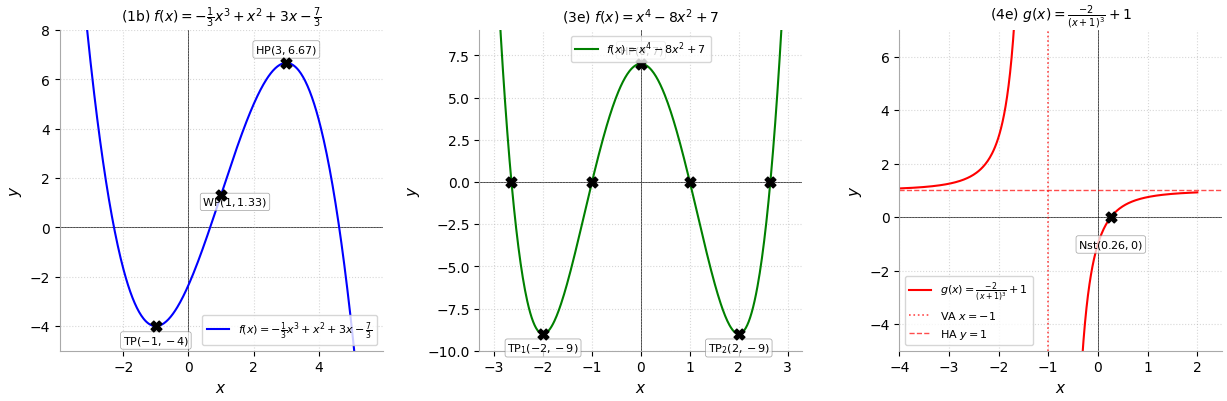
\includegraphics[width=0.8\textwidth]{grafiken/uebergreifend_alle_graphen.png.png}
    \captionof{figure}{Graphen der untersuchten Funktionen: (1b) $f(x) = -\frac{1}{3}x^3 + x^2 + 3x - \frac{7}{3}$, (3e) $f(x) = x^4 - 8x^2 + 7$, und (4e) $g(x) = \frac{-2}{(x+1)^3} + 1$.}
    \label{fig:uebergreifend_alle_graphen}
\end{center}

\end{loesungsumgebung}




\begin{aufgabenumgebung}{Produktregel trainieren}
Leite die folgenden Funktionen mit der Produktregel ab und vereinfache die Ergebnisse so weit wie möglich. Kontrolliere deine Ergebnisse für die ersten beiden Aufgaben, indem du die Terme zuerst ausmultiplizierst und dann ableitest.
\begin{enumerate}
    \item $f(x) = (x+2)(3x-4)$
    \item $g(x) = x^2(x^3+5x)$
    \item $h(t) = (t^2-1)(t^2+1)$ (Erkennst du hier eine binomische Formel, die das Ausmultiplizieren erleichtert?)
    \item $k(x) = (2x^3-x)(x^2+x+1)$
    \item $m(a) = (a^2+1)(a-1)$ (Leite nach $a$ ab.)
\end{enumerate}
\end{aufgabenumgebung}

\begin{loesungsumgebung}[loes:produktregel-trainieren]{Produktregel trainieren}
Wir verwenden die Produktregel $f'(x) = u'(x)v(x) + u(x)v'(x)$, um die Ableitungen zu bestimmen.

\begin{enumerate}[label=(\alph*)]
    \item \textbf{Funktion $f(x) = (x+2)(3x-4)$}
    \begin{itemize}
        \item \textbf{Mit Produktregel:} \\
        Sei $u(x) = x+2 \Rightarrow u'(x) = 1$. \\
        Sei $v(x) = 3x-4 \Rightarrow v'(x) = 3$.
        \begin{align*}
        f'(x) &= u'(x)v(x) + u(x)v'(x) \\
              &= 1 \cdot (3x-4) + (x+2) \cdot 3 \\
              &= 3x - 4 + 3x + 6 \\
              &= \mathbf{6x + 2}
        \end{align*}
        \item \textbf{Kontrolle durch Ausmultiplizieren:}
        $f(x) = (x+2)(3x-4) = 3x^2 - 4x + 6x - 8 = 3x^2 + 2x - 8$.
        $f'(x) = \frac{d}{dx}(3x^2 + 2x - 8) = 6x + 2$.
        Die Ergebnisse stimmen überein.
    \end{itemize}

    \item \textbf{Funktion $g(x) = x^2(x^3+5x)$}
    \begin{itemize}
        \item \textbf{Mit Produktregel:} \\
        Sei $u(x) = x^2 \Rightarrow u'(x) = 2x$. \\
        Sei $v(x) = x^3+5x \Rightarrow v'(x) = 3x^2+5$.
        \begin{align*}
        g'(x) &= u'(x)v(x) + u(x)v'(x) \\
              &= 2x(x^3+5x) + x^2(3x^2+5) \\
              &= 2x^4 + 10x^2 + 3x^4 + 5x^2 \\
              &= \mathbf{5x^4 + 15x^2}
        \end{align*}
        \item \textbf{Kontrolle durch Ausmultiplizieren:}
        $g(x) = x^2(x^3+5x) = x^5 + 5x^3$.
        $g'(x) = \frac{d}{dx}(x^5 + 5x^3) = 5x^4 + 15x^2$.
        Die Ergebnisse stimmen überein.
    \end{itemize}

    \item \textbf{Funktion $h(t) = (t^2-1)(t^2+1)$} \\
    \textit{Tipp:} Dies ist die 3. binomische Formel: $(A-B)(A+B) = A^2-B^2$.
    $h(t) = (t^2)^2 - 1^2 = t^4 - 1$.
    Ableiten der vereinfachten Form:
    $h'(t) = \frac{d}{dt}(t^4 - 1) = \mathbf{4t^3}$.
    \textit{Zur Übung auch mit Produktregel:} \\
    Sei $u(t) = t^2-1 \Rightarrow u'(t) = 2t$. \\
    Sei $v(t) = t^2+1 \Rightarrow v'(t) = 2t$.
    \begin{align*}
    h'(t) &= u'(t)v(t) + u(t)v'(t) \\
          &= 2t(t^2+1) + (t^2-1)(2t) \\
          &= 2t^3 + 2t + 2t^3 - 2t \\
          &= 4t^3
    \end{align*}
    Die Ergebnisse stimmen überein. Das Ausmultiplizieren war hier schneller.

    \item \textbf{Funktion $k(x) = (2x^3-x)(x^2+x+1)$}
    \begin{itemize}
        \item \textbf{Mit Produktregel:} \\
        Sei $u(x) = 2x^3-x \Rightarrow u'(x) = 6x^2-1$. \\
        Sei $v(x) = x^2+x+1 \Rightarrow v'(x) = 2x+1$.
        \begin{align*}
        k'(x) &= u'(x)v(x) + u(x)v'(x) \\
              &= (6x^2-1)(x^2+x+1) + (2x^3-x)(2x+1) \\
              &= (6x^4 + 6x^3 + 6x^2 - x^2 - x - 1) + (4x^4 + 2x^3 - 2x^2 - x) \\
              &= (6x^4 + 6x^3 + 5x^2 - x - 1) + (4x^4 + 2x^3 - 2x^2 - x) \\
              &= \mathbf{10x^4 + 8x^3 + 3x^2 - 2x - 1}
        \end{align*}
    \end{itemize}

    \item \textbf{Funktion $m(a) = (a^2+1)(a-1)$ (Ableitung nach $a$)}
    \begin{itemize}
        \item \textbf{Mit Produktregel:} \\
        Sei $u(a) = a^2+1 \Rightarrow u'(a) = 2a$. \\
        Sei $v(a) = a-1 \Rightarrow v'(a) = 1$.
        \begin{align*}
        m'(a) &= u'(a)v(a) + u(a)v'(a) \\
               &= 2a(a-1) + (a^2+1)(1) \\
               &= 2a^2 - 2a + a^2 + 1 \\
               &= \mathbf{3a^2 - 2a + 1}
        \end{align*}
        \textit{Kontrolle durch Ausmultiplizieren:}
        $m(a) = a^3 - a^2 + a - 1$.
        $m'(a) = 3a^2 - 2a + 1$. (Stimmt überein)
    \end{itemize}
\end{enumerate}

\end{loesungsumgebung}

\begin{aufgabenumgebung}[A:ProduktregelAnwendung]{Anwendung der Produktregel in einer Kurvendiskussion (vereinfacht)}
Gegeben sei die Funktion $f(x) = x \cdot (x-3)^2$.
\begin{enumerate}
    \item \textbf{Definitionsbereich und Verhalten im Unendlichen:} Bestimme $D_f$ und untersuche $\lim_{x \to \pm\infty} f(x)$.
    \item \textbf{Nullstellen:} Bestimme die Nullstellen von $f(x)$ direkt aus der faktorisierten Form. Welche Vielfachheit haben sie? Was bedeutet das für den Graphen?
    \item \textbf{Erste Ableitung mit Produktregel:}
        Identifiziere $u(x)=x$ und $v(x)=(x-3)^2$. 
        Bilde $f'(x)$ mit der Produktregel. Vereinfache $f'(x)$ so weit wie möglich (Tipp: $(x-3)$ ausklammern).
    \item \textbf{Extremstellen:} Bestimme die Nullstellen von $f'(x)$. Untersuche das Vorzeichen von $f'(x)$ (Monotonieintervalle), um die Art der Extremstellen zu bestimmen. Berechne die y-Koordinaten der Extrempunkte.
    \item \textbf{Skizze:} Skizziere den Graphen von $f(x)$ unter Verwendung deiner Ergebnisse.
\end{enumerate}
Diese Aufgabe zeigt, wie die Produktregel auch bei der Analyse von Polynomfunktionen nützlich sein kann, besonders wenn sie in faktorisierter Form vorliegen oder entstehen.
\end{aufgabenumgebung}

\begin{loesungsumgebung}[loes:A:ProduktregelAnwendung]{Anwendung der Produktregel in einer Kurvendiskussion}
Wir untersuchen die Funktion $f(x) = x \cdot (x-3)^2$.

\begin{enumerate}[label=(\alph*)]
    \item \textbf{Definitionsbereich und Verhalten im Unendlichen:}
    \begin{itemize}
        \item \textbf{Definitionsbereich ($D_f$):} Da $f(x)$ eine Polynomfunktion ist (nach Ausmultiplizieren $f(x) = x(x^2-6x+9) = x^3-6x^2+9x$), ist der Definitionsbereich $\mathbf{D_f = \mathbb{R}}$.
        \item \textbf{Verhalten im Unendlichen ($\lim_{x \to \pm\infty} f(x)$):}
        Der Leitterm der ausmultiplizierten Form $x^3-6x^2+9x$ ist $x^3$.
        Für $x \to \infty$: $\lim_{x \to \infty} f(x) = \lim_{x \to \infty} x^3 = \mathbf{+\infty}$.
        Für $x \to -\infty$: $\lim_{x \to -\infty} f(x) = \lim_{x \to -\infty} x^3 = \mathbf{-\infty}$.
        (Der Graph verläuft von links unten nach rechts oben).
    \end{itemize}

    \item \textbf{Nullstellen:}
    Wir setzen $f(x)=0$: $x \cdot (x-3)^2 = 0$.
    Nach dem Satz vom Nullprodukt gilt:
    \begin{itemize}
        \item $x_1 = 0$. Dies ist eine \textbf{einfache Nullstelle} (der Faktor $x$ hat den Exponenten 1). Der Graph schneidet hier die x-Achse.
        \item $(x-3)^2 = 0 \Rightarrow x-3=0 \Rightarrow x_2 = 3$. Dies ist eine \textbf{doppelte Nullstelle} (der Faktor $(x-3)$ hat den Exponenten 2). Der Graph berührt hier die x-Achse.
    \end{itemize}
    Die Nullstellen sind $N_1(0|0)$ und $N_2(3|0)$.

    \item \textbf{Erste Ableitung mit Produktregel:}
    Sei $u(x)=x$ und $v(x)=(x-3)^2$.
    Dann ist $u'(x)=1$.
    Für $v'(x)$ verwenden wir den Tipp oder leiten ausmultipliziert ab: $v(x) = x^2-6x+9 \Rightarrow v'(x) = 2x-6 = 2(x-3)$.
    Nach der Produktregel $f'(x) = u'(x)v(x) + u(x)v'(x)$:
    \begin{align*}
    f'(x) &= 1 \cdot (x-3)^2 + x \cdot [2(x-3)] \\
          &= (x-3)^2 + 2x(x-3)
    \end{align*}
    Wir klammern $(x-3)$ aus:
    \begin{align*}
    f'(x) &= (x-3) \cdot [(x-3) + 2x] \\
          &= (x-3) \cdot (3x-3) \\
          &= \mathbf{3(x-3)(x-1)}
    \end{align*}

    \item \textbf{Extremstellen:}
    Notwendige Bedingung: $f'(x_E)=0$.
    $3(x-3)(x-1) = 0$.
    Die Kandidaten für Extremstellen sind $x_{E1} = 1$ und $x_{E2} = 3$.
    Untersuchung des Vorzeichens von $f'(x) = 3(x-1)(x-3)$:
    Der Graph von $f'(x)$ ist eine nach oben geöffnete Parabel mit Nullstellen bei $1$ und $3$.
    \begin{itemize}
        \item Für $x < 1$ (z.B. $x=0$): $f'(0) = 3(-1)(-3) = 9 > 0 \implies f(x)$ ist streng monoton steigend.
        \item Für $1 < x < 3$ (z.B. $x=2$): $f'(2) = 3(1)(-1) = -3 < 0 \implies f(x)$ ist streng monoton fallend.
        \item Für $x > 3$ (z.B. $x=4$): $f'(4) = 3(3)(1) = 9 > 0 \implies f(x)$ ist streng monoton steigend.
    \end{itemize}
    Art und Koordinaten der Extrempunkte:
    \begin{itemize}
        \item Bei $x_{E1} = 1$: Vorzeichenwechsel von $f'(x)$ von $+$ nach $- \Rightarrow$ Lokaler Hochpunkt.
        $y_{E1} = f(1) = 1 \cdot (1-3)^2 = 1 \cdot (-2)^2 = 4$.
        $\rightarrow \mathbf{HP(1|4)}$.
        \item Bei $x_{E2} = 3$: Vorzeichenwechsel von $f'(x)$ von $-$ nach $+ \Rightarrow$ Lokaler Tiefpunkt.
        $y_{E2} = f(3) = 3 \cdot (3-3)^2 = 3 \cdot 0^2 = 0$.
        $\rightarrow \mathbf{TP(3|0)}$. (Dies ist auch die doppelte Nullstelle, was konsistent ist).
    \end{itemize}

    \item \textbf{Skizze:}
    Der Graph der Funktion $f(x) = x(x-3)^2$ ist ein Polynom 3. Grades.
    \begin{itemize}
        \item Er verläuft von links unten ($x \to -\infty, f(x) \to -\infty$) nach rechts oben ($x \to \infty, f(x) \to \infty$).
        \item Er schneidet die x-Achse bei $x=0$ (einfache Nullstelle) und berührt die x-Achse bei $x=3$ (doppelte Nullstelle, gleichzeitig Tiefpunkt).
        \item Er hat einen lokalen Hochpunkt bei $HP(1|4)$.
        \item Der y-Achsenabschnitt ist $(0|0)$.
    \end{itemize}
    \begin{center}
    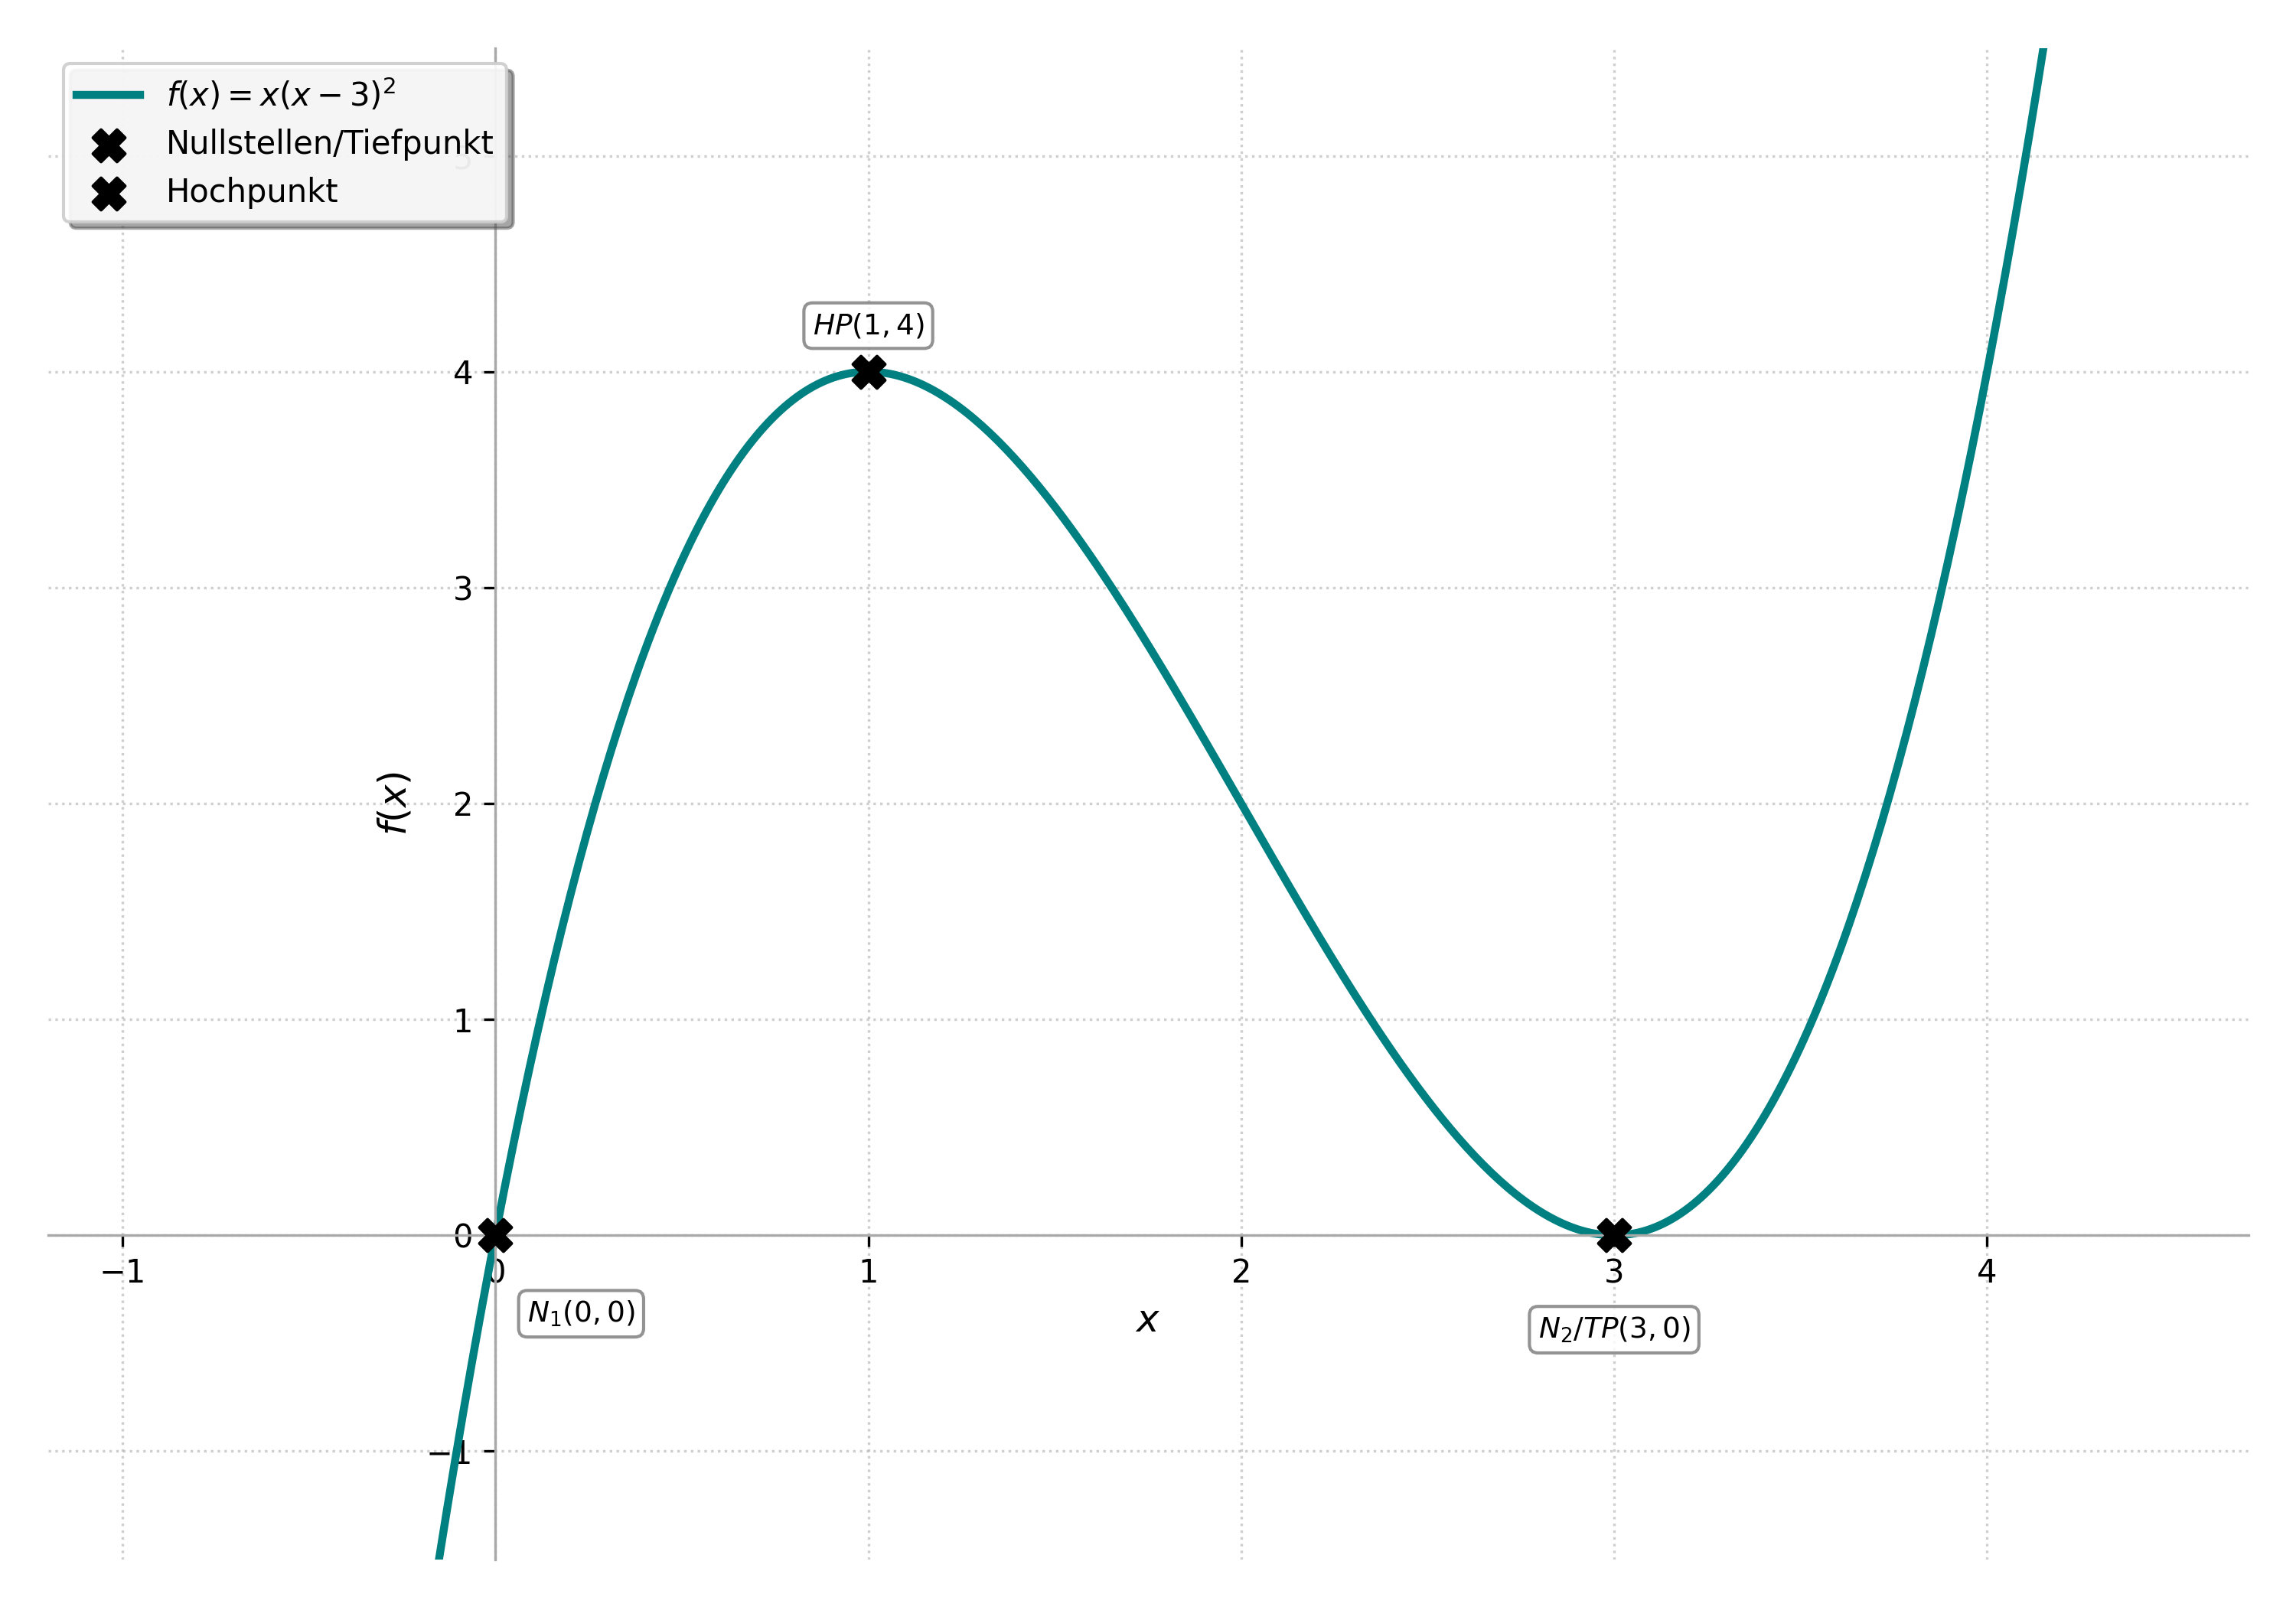
\includegraphics[width=0.8\textwidth]{grafiken/f_produktregel_anwendung_graph.png}
    % --- Beschreibung der Skizze ---
    % Die Skizze zeigt den Graphen eines Polynoms 3. Grades.
    % Nullstellen: (0|0) - Schnittpunkt; (3|0) - Berührpunkt (Tiefpunkt).
    % Lokaler Hochpunkt: (1|4).
    % Verlauf: Kommt von links unten, steigt zum HP(1|4), fällt zum TP(3|0) (berührt x-Achse), steigt dann nach rechts oben.
    \captionof{figure}{Graph der Funktion $f(x) = x(x-3)^2$.}
    \label{fig:f_produktregel_anwendung_graph}
    \end{center}
\end{enumerate}

\end{loesungsumgebung}


\begin{aufgabenumgebung}{Quotientenregel trainieren}
Leite die folgenden Funktionen mit der Quotientenregel ab und vereinfache die Zähler der Ergebnisse so weit wie möglich. Gib auch den Definitionsbereich der ursprünglichen Funktion an.
\begin{enumerate}
    \item $f(x) = \frac{x}{x+1}$
    \item $g(x) = \frac{3x-2}{x^2}$ (Tipp: Dies könnte man auch als $g(x) = (3x-2)x^{-2}$ mit der Produktregel oder nach Aufteilen des Bruchs $\frac{3x}{x^2} - \frac{2}{x^2} = \frac{3}{x} - \frac{2}{x^2}$ mit Potenz-/Faktorregeln ableiten. Vergleiche die Ergebnisse!)
    \item $h(t) = \frac{t^2+2t}{t-1}$
    \item $k(x) = \frac{5}{2x+3}$ (Hier ist $u(x)=5$, also $u'(x)=0$. Was bedeutet das für die Formel?)
\end{enumerate}
\end{aufgabenumgebung}



\begin{loesungsumgebung}[loes:quotientenregel-trainieren]{Quotientenregel trainieren}
Wir verwenden die Quotientenregel $f'(x) = \frac{u'(x)v(x) - u(x)v'(x)}{[v(x)]^2}$, um die Ableitungen zu bestimmen.

\begin{enumerate}[label=(\alph*)]
    \item \textbf{Funktion $f(x) = \frac{x}{x+1}$}
    \begin{itemize}
        \item \textbf{Definitionsbereich:} Der Nenner darf nicht Null sein: $x+1 \neq 0 \Rightarrow x \neq -1$. $D_f = \mathbb{R} \setminus \{-1\}$.
        \item \textbf{Ableitung mit Quotientenregel:} \\
        Sei $u(x) = x \Rightarrow u'(x) = 1$. \\
        Sei $v(x) = x+1 \Rightarrow v'(x) = 1$.
        \begin{align*}
        f'(x) &= \frac{u'(x)v(x) - u(x)v'(x)}{[v(x)]^2} \\
              &= \frac{1 \cdot (x+1) - x \cdot 1}{(x+1)^2} \\
              &= \frac{x+1-x}{(x+1)^2} \\
              &= \mathbf{\frac{1}{(x+1)^2}}
        \end{align*}
    \end{itemize}

    \item \textbf{Funktion $g(x) = \frac{3x-2}{x^2}$}
    \begin{itemize}
        \item \textbf{Definitionsbereich:} $x^2 \neq 0 \Rightarrow x \neq 0$. $D_g = \mathbb{R} \setminus \{0\}$.
        \item \textbf{Ableitung mit Quotientenregel:} \\
        Sei $u(x) = 3x-2 \Rightarrow u'(x) = 3$. \\
        Sei $v(x) = x^2 \Rightarrow v'(x) = 2x$.
        \begin{align*}
        g'(x) &= \frac{3 \cdot x^2 - (3x-2) \cdot 2x}{(x^2)^2} \\
              &= \frac{3x^2 - (6x^2 - 4x)}{x^4} \\
              &= \frac{3x^2 - 6x^2 + 4x}{x^4} \\
              &= \frac{-3x^2 + 4x}{x^4} \\
              &= \frac{x(-3x + 4)}{x \cdot x^3} \quad (\text{für } x \neq 0) \\
              &= \mathbf{\frac{-3x + 4}{x^3}} \quad \text{oder } \mathbf{-\frac{3}{x^2} + \frac{4}{x^3}}
        \end{align*}
        \item \textbf{Vergleich mit alternativen Methoden (Tipp):}
        \begin{itemize}
            \item \textit{Als Produkt $g(x) = (3x-2)x^{-2}$:} \\
            $u(x)=3x-2 \Rightarrow u'(x)=3$. $w(x)=x^{-2} \Rightarrow w'(x)=-2x^{-3}$.
            $g'(x) = 3x^{-2} + (3x-2)(-2x^{-3}) = \frac{3}{x^2} - \frac{6x}{x^3} + \frac{4}{x^3} = \frac{3}{x^2} - \frac{6}{x^2} + \frac{4}{x^3} = -\frac{3}{x^2} + \frac{4}{x^3} = \frac{-3x+4}{x^3}$. (Stimmt überein)
            \item \textit{Nach Aufteilen des Bruchs $g(x) = \frac{3x}{x^2} - \frac{2}{x^2} = 3x^{-1} - 2x^{-2}$:} \\
            $g'(x) = 3(-1)x^{-2} - 2(-2)x^{-3} = -3x^{-2} + 4x^{-3} = -\frac{3}{x^2} + \frac{4}{x^3} = \frac{-3x+4}{x^3}$. (Stimmt überein)
        \end{itemize}
    \end{itemize}

    \item \textbf{Funktion $h(t) = \frac{t^2+2t}{t-1}$}
    \begin{itemize}
        \item \textbf{Definitionsbereich:} $t-1 \neq 0 \Rightarrow t \neq 1$. $D_h = \mathbb{R} \setminus \{1\}$.
        \item \textbf{Ableitung mit Quotientenregel:} \\
        Sei $u(t) = t^2+2t \Rightarrow u'(t) = 2t+2$. \\
        Sei $v(t) = t-1 \Rightarrow v'(t) = 1$.
        \begin{align*}
        h'(t) &= \frac{(2t+2)(t-1) - (t^2+2t)(1)}{(t-1)^2} \\
              &= \frac{(2t^2 - 2t + 2t - 2) - (t^2+2t)}{(t-1)^2} \\
              &= \frac{2t^2 - 2 - t^2 - 2t}{(t-1)^2} \\
              &= \mathbf{\frac{t^2 - 2t - 2}{(t-1)^2}}
        \end{align*}
    \end{itemize}

    \item \textbf{Funktion $k(x) = \frac{5}{2x+3}$}
    \begin{itemize}
        \item \textbf{Definitionsbereich:} $2x+3 \neq 0 \Rightarrow 2x \neq -3 \Rightarrow x \neq -\frac{3}{2}$. $D_k = \mathbb{R} \setminus \{-\frac{3}{2}\}$.
        \item \textbf{Ableitung mit Quotientenregel:} \\
        Sei $u(x) = 5 \Rightarrow u'(x) = 0$. \\
        Sei $v(x) = 2x+3 \Rightarrow v'(x) = 2$.
        \begin{align*}
        k'(x) &= \frac{0 \cdot (2x+3) - 5 \cdot 2}{(2x+3)^2} \\
              &= \frac{0 - 10}{(2x+3)^2} \\
              &= \mathbf{\frac{-10}{(2x+3)^2}}
        \end{align*}
        \textit{Anmerkung:} Da $u(x)$ eine Konstante ist, wird der erste Term im Zähler der Quotientenregel ($u'v$) Null. Die Formel vereinfacht sich zu $k'(x) = \frac{-uv'}{v^2}$. Dies entspricht auch der Ableitung mittels Kettenregel für $k(x) = 5(2x+3)^{-1}$: $k'(x) = 5 \cdot (-1)(2x+3)^{-2} \cdot 2 = -10(2x+3)^{-2}$.
    \end{itemize}
\end{enumerate}

\end{loesungsumgebung}



\begin{aufgabenumgebung}{Anwendung der neuen Regeln in Kontexten}
\begin{enumerate}
    \item \textbf{Umsatzfunktion:} Ein Unternehmen verkauft ein Produkt. Die Preis-Absatz-Funktion (Nachfragefunktion) sei $p(x) = 100 - 0.5x$, wobei $x$ die verkaufte Menge und $p(x)$ der Preis pro Stück ist. Der Umsatz $U(x)$ ist Preis mal Menge, also $U(x) = p(x) \cdot x = (100-0.5x)x$.
        \begin{itemize}
            \item Bestimme die Umsatzfunktion $U(x)$.
            \item Bilde die erste Ableitung $U'(x)$ (Grenzerlös). Du kannst dies tun, indem du $U(x)$ zuerst ausmultiplizierst oder indem du die Produktregel auf $p(x) \cdot x$ anwendest. Vergleiche beide Wege.
            \item Bei welcher Verkaufsmenge $x$ wird der Grenzerlös Null? Was könnte das für den Gesamtumsatz bedeuten?
        \end{itemize}
    \item \textbf{Durchschnittskosten:} Die Kostenfunktion eines Unternehmens sei $K(x) = 0.1x^3 - 2x^2 + 50x + 100$. Die Durchschnittskosten (Stückkosten) sind $k(x) = \frac{K(x)}{x}$.
        \begin{itemize}
            \item Schreibe die Funktion für die Durchschnittskosten $k(x)$ auf.
            \item Bilde die erste Ableitung $k'(x)$ mit der Quotientenregel.
            \item (Für Experten): Versuche, die Stelle zu finden, an der die Durchschnittskosten minimal sind (also $k'(x)=0$ setzen und nach $x$ auflösen – das kann hier schwierig werden, aber der Ansatz ist wichtig).
        \end{itemize}
\end{enumerate}
\end{aufgabenumgebung}



\begin{loesungsumgebung}[loes:anwendung-produkt-quotientenregel-kontext]{Anwendung der neuen Regeln in Kontexten}

\begin{enumerate}[label=(\alph*)]
    \item \textbf{Umsatzfunktion:}
    Gegeben ist die Preis-Absatz-Funktion $p(x) = 100 - 0.5x$. Der Umsatz ist $U(x) = p(x) \cdot x$.
    \begin{itemize}
        \item \textbf{Bestimme die Umsatzfunktion $U(x)$:}
        $U(x) = (100 - 0.5x) \cdot x = \mathbf{100x - 0.5x^2}$.

        \item \textbf{Bilde die erste Ableitung $U'(x)$ (Grenzerlös):}
        \textit{Weg 1: Ableiten der ausmultiplizierten Form}
        $U(x) = 100x - 0.5x^2$.
        $U'(x) = \frac{d}{dx}(100x - 0.5x^2) = 100 - 0.5 \cdot 2x = \mathbf{100 - x}$.

        \textit{Weg 2: Anwendung der Produktregel auf $U(x) = (100-0.5x)x$}
        Sei $u(x) = 100-0.5x \Rightarrow u'(x) = -0.5$.
        Sei $v(x) = x \Rightarrow v'(x) = 1$.
        $U'(x) = u'(x)v(x) + u(x)v'(x) = (-0.5)(x) + (100-0.5x)(1)$
        $U'(x) = -0.5x + 100 - 0.5x = \mathbf{100 - x}$.
        \textit{Vergleich:} Beide Wege führen zum selben Ergebnis.

        \item \textbf{Bei welcher Verkaufsmenge $x$ wird der Grenzerlös Null? Was könnte das für den Gesamtumsatz bedeuten?}
        Setze $U'(x) = 0$:
        $100 - x = 0 \Rightarrow x = 100$.
        Der Grenzerlös wird bei einer Verkaufsmenge von $\mathbf{x=100}$ Null.
        \textit{Bedeutung:} Wenn der Grenzerlös Null ist, bedeutet das, dass eine weitere verkaufte Einheit keinen zusätzlichen Umsatz mehr generiert (oder der zusätzliche Umsatz ist vernachlässigbar klein). Da die Umsatzfunktion $U(x) = -0.5x^2 + 100x$ eine nach unten geöffnete Parabel ist ($a=-0.5 < 0$), befindet sich an der Stelle, an der die erste Ableitung Null ist, das \textbf{Maximum des Gesamtumsatzes}. Bei einer Verkaufsmenge von 100 Stück ist der Umsatz also maximal.
    \end{itemize}

    \item \textbf{Durchschnittskosten:}
    Kostenfunktion $K(x) = 0.1x^3 - 2x^2 + 50x + 100$. Durchschnittskosten $k(x) = \frac{K(x)}{x}$.
    \begin{itemize}
        \item \textbf{Schreibe die Funktion für die Durchschnittskosten $k(x)$ auf:}
        $k(x) = \frac{0.1x^3 - 2x^2 + 50x + 100}{x}$.
        Für den Definitionsbereich $x>0$ (da $x$ eine Menge ist) können wir auch schreiben:
        $k(x) = 0.1x^2 - 2x + 50 + \frac{100}{x}$.

        \item \textbf{Bilde die erste Ableitung $k'(x)$ mit der Quotientenregel:}
        Für $k(x) = \frac{K(x)}{x}$:
        Sei $u(x) = K(x) = 0.1x^3 - 2x^2 + 50x + 100 \Rightarrow u'(x) = K'(x) = 0.3x^2 - 4x + 50$.
        Sei $v(x) = x \Rightarrow v'(x) = 1$.
        \begin{align*}
        k'(x) &= \frac{u'(x)v(x) - u(x)v'(x)}{[v(x)]^2} \\
              &= \frac{(0.3x^2 - 4x + 50) \cdot x - (0.1x^3 - 2x^2 + 50x + 100) \cdot 1}{x^2} \\
              &= \frac{0.3x^3 - 4x^2 + 50x - 0.1x^3 + 2x^2 - 50x - 100}{x^2} \\
              &= \frac{0.2x^3 - 2x^2 - 100}{x^2} \\
              &= \mathbf{0.2x - 2 - \frac{100}{x^2}} \quad (\text{für } x \neq 0)
        \end{align*}
        \textit{Kontrolle mit $k(x) = 0.1x^2 - 2x + 50 + 100x^{-1}$:}
        $k'(x) = 0.2x - 2 - 100x^{-2} = 0.2x - 2 - \frac{100}{x^2}$. (Stimmt überein).

        \item \textbf{(Für Experten): Stelle finden, an der die Durchschnittskosten minimal sind ($k'(x)=0$):}
        Wir setzen $k'(x) = 0$:
        $0.2x - 2 - \frac{100}{x^2} = 0$.
        Multiplikation mit $x^2$ (für $x \neq 0$):
        $0.2x^3 - 2x^2 - 100 = 0$.
        Multiplikation mit 5, um ganzzahlige Koeffizienten zu erhalten (optional):
        $x^3 - 10x^2 - 500 = 0$.
        Dies ist eine kubische Gleichung. Ihre exakte algebraische Lösung ist nicht trivial und erfordert typischerweise das Raten einer Nullstelle (Teiler von 500) oder numerische Verfahren.
        Wenn $P(x) = x^3 - 10x^2 - 500$:
        $P(10) = 1000 - 1000 - 500 = -500$.
        $P(11) = 1331 - 1210 - 500 = -379$.
        $P(12) = 1728 - 1440 - 500 = -212$.
        $P(13) = 2197 - 1690 - 500 = 7$.
        Da $P(12) < 0$ und $P(13) > 0$, liegt eine Nullstelle (und somit eine potenzielle Stelle minimaler Durchschnittskosten) zwischen $x=12$ und $x=13$. Die exakte Stelle müsste numerisch oder mit fortgeschritteneren Methoden zur Lösung kubischer Gleichungen bestimmt werden. Der Ansatz, $k'(x)=0$ zu setzen, ist der korrekte Weg, um das Minimum der Durchschnittskosten zu finden. (Dieser Punkt ist auch bekannt als das Betriebsoptimum, wo die Grenzkosten $K'(x)$ die Durchschnittskosten $k(x)$ schneiden).
    \end{itemize}
\end{enumerate}

\end{loesungsumgebung}

\begin{aufgabenumgebung}{Kettenregel trainieren}
Leite die folgenden Funktionen mit der Kettenregel ab. Identifiziere zuerst sorgfältig die äußere und die innere Funktion.
\begin{enumerate}
    \item $f(x) = (x^2+1)^4$
    \item $g(x) = (5-3x)^7$
    \item $h(t) = \sqrt{t^2+3t}$ (Tipp: $\sqrt{u} = u^{1/2}$)
    \item $k(x) = \frac{1}{(x^3-2x)^2}$ (Tipp: $k(x) = (x^3-2x)^{-2}$)
    \item $m(x) = (ax^2+b)^n$ (wobei $a,b,n$ Konstanten sind. Was ist die Ableitung?)
\end{enumerate}
\end{aufgabenumgebung}

\begin{loesungsumgebung}[loes:kettenregel-trainieren]{Kettenregel trainieren}
Wir identifizieren jeweils die äußere Funktion $a(u)$ und die innere Funktion $u=i(x)$, bilden deren Ableitungen $a'(u)$ und $i'(x)$ und wenden dann die Kettenregel $f'(x) = a'(i(x)) \cdot i'(x)$ an.

\begin{enumerate}[label=(\alph*)]
    \item \textbf{Funktion $f(x) = (x^2+1)^4$}
    \begin{itemize}
        \item Äußere Funktion: $a(u) = u^4 \Rightarrow a'(u) = 4u^3$.
        \item Innere Funktion: $i(x) = x^2+1 \Rightarrow i'(x) = 2x$.
    \end{itemize}
    Anwendung der Kettenregel:
    \begin{align*}
    f'(x) &= a'(i(x)) \cdot i'(x) \\
          &= 4(x^2+1)^3 \cdot (2x) \\
          &= \mathbf{8x(x^2+1)^3}
    \end{align*}

    \item \textbf{Funktion $g(x) = (5-3x)^7$}
    \begin{itemize}
        \item Äußere Funktion: $a(u) = u^7 \Rightarrow a'(u) = 7u^6$.
        \item Innere Funktion: $i(x) = 5-3x \Rightarrow i'(x) = -3$.
    \end{itemize}
    Anwendung der Kettenregel:
    \begin{align*}
    g'(x) &= a'(i(x)) \cdot i'(x) \\
          &= 7(5-3x)^6 \cdot (-3) \\
          &= \mathbf{-21(5-3x)^6}
    \end{align*}

    \item \textbf{Funktion $h(t) = \sqrt{t^2+3t}$} \\
    Tipp: $\sqrt{u} = u^{1/2}$. Also $h(t) = (t^2+3t)^{1/2}$.
    \begin{itemize}
        \item Äußere Funktion: $a(u) = u^{1/2} \Rightarrow a'(u) = \frac{1}{2}u^{-1/2} = \frac{1}{2\sqrt{u}}$.
        \item Innere Funktion: $i(t) = t^2+3t \Rightarrow i'(t) = 2t+3$.
    \end{itemize}
    Anwendung der Kettenregel:
    \begin{align*}
    h'(t) &= a'(i(t)) \cdot i'(t) \\
          &= \frac{1}{2\sqrt{t^2+3t}} \cdot (2t+3) \\
          &= \mathbf{\frac{2t+3}{2\sqrt{t^2+3t}}}
    \end{align*}

    \item \textbf{Funktion $k(x) = \frac{1}{(x^3-2x)^2}$} \\
    Tipp: $k(x) = (x^3-2x)^{-2}$.
    \begin{itemize}
        \item Äußere Funktion: $a(u) = u^{-2} \Rightarrow a'(u) = -2u^{-3} = \frac{-2}{u^3}$.
        \item Innere Funktion: $i(x) = x^3-2x \Rightarrow i'(x) = 3x^2-2$.
    \end{itemize}
    Anwendung der Kettenregel:
    \begin{align*}
    k'(x) &= a'(i(x)) \cdot i'(x) \\
          &= \frac{-2}{(x^3-2x)^3} \cdot (3x^2-2) \\
          &= \mathbf{\frac{-2(3x^2-2)}{(x^3-2x)^3}} \quad \text{oder} \quad \mathbf{\frac{-6x^2+4}{(x^3-2x)^3}}
    \end{align*}

    \item \textbf{Funktion $m(x) = (ax^2+b)^n$} (wobei $a,b,n$ Konstanten sind)
    \begin{itemize}
        \item Äußere Funktion: $a_u(u) = u^n \Rightarrow a_u'(u) = nu^{n-1}$. (Der Index $u$ bei $a_u$ dient zur Unterscheidung vom Parameter $a$).
        \item Innere Funktion: $i(x) = ax^2+b \Rightarrow i'(x) = 2ax$ (da $b$ eine Konstante ist).
    \end{itemize}
    Anwendung der Kettenregel:
    \begin{align*}
    m'(x) &= a_u'(i(x)) \cdot i'(x) \\
           &= n(ax^2+b)^{n-1} \cdot (2ax) \\
           &= \mathbf{2anx(ax^2+b)^{n-1}}
    \end{align*}
    Dies ist die verallgemeinerte Potenzregel für eine innere lineare oder quadratische Funktion.
\end{enumerate}

\end{loesungsumgebung}



\begin{aufgabenumgebung}[A:KombinierteAnwendung]{Kombinierte Anwendung der Ableitungsregeln}
Leite die folgenden Funktionen ab. Gib an, welche Regeln du in welcher Reihenfolge anwendest.
\begin{enumerate}
    \item $f(x) = x^2 \cdot (2x+1)^3$ (Produkt- und Kettenregel)
    \item $g(x) = \frac{(x^2-1)^2}{x}$ (Quotienten- und Kettenregel, oder erst Zähler ausmultiplizieren)
    \item $h(t) = t \cdot \sqrt{1-t^2}$ (Produkt- und Kettenregel)
    \item \textbf{Für Tüftler:} Untersuche die Funktion $f(x) = x \cdot (x-4)^3$ auf Nullstellen, Monotonie und Extrempunkte. Skizziere den Graphen. (Diese Funktion ähnelt der Aufgabe \ref{A:ProduktregelAnwendung}, erfordert aber nun die Kettenregel für $v'(x)$.)
\end{enumerate}
\end{aufgabenumgebung}

\begin{loesungsumgebung}[loes:A:KombinierteAnwendung]{Kombinierte Anwendung der Ableitungsregeln}

\begin{enumerate}[label=(\alph*)]
    \item \textbf{Funktion $f(x) = x^2 \cdot (2x+1)^3$} \\
    Wir wenden die \textbf{Produktregel} an: $f'(x) = u'(x)v(x) + u(x)v'(x)$.
    Sei $u(x) = x^2 \Rightarrow u'(x) = 2x$.
    Sei $v(x) = (2x+1)^3$. Für $v'(x)$ benötigen wir die \textbf{Kettenregel}:
    Äußere Funktion $a_v(w) = w^3 \Rightarrow a_v'(w) = 3w^2$.
    Innere Funktion $i_v(x) = 2x+1 \Rightarrow i_v'(x) = 2$.
    Also $v'(x) = a_v'(i_v(x)) \cdot i_v'(x) = 3(2x+1)^2 \cdot 2 = 6(2x+1)^2$.
    \begin{align*}
    f'(x) &= (2x) \cdot (2x+1)^3 + (x^2) \cdot [6(2x+1)^2] \\
          &= (2x+1)^2 [2x(2x+1) + 6x^2] \quad (\text{Ausklammern von } (2x+1)^2) \\
          &= (2x+1)^2 [4x^2 + 2x + 6x^2] \\
          &= (2x+1)^2 (10x^2 + 2x) \\
          &= (2x+1)^2 \cdot 2x(5x+1) \\
          &= \mathbf{2x(5x+1)(2x+1)^2}
    \end{align*}
    \textit{Verwendete Regeln: Produktregel, Kettenregel, Potenzregel, Faktorregel, Summenregel.}

    \item \textbf{Funktion $g(x) = \frac{(x^2-1)^2}{x}$} \\
    \textit{Weg 1: Mit Quotienten- und Kettenregel.} $g(x) = \frac{u(x)}{v(x)}$.
    Sei $u(x) = (x^2-1)^2$. Für $u'(x)$ Kettenregel: $a_u(w)=w^2 \Rightarrow a_u'(w)=2w$; $i_u(x)=x^2-1 \Rightarrow i_u'(x)=2x$.
    Also $u'(x) = 2(x^2-1) \cdot 2x = 4x(x^2-1)$.
    Sei $v(x) = x \Rightarrow v'(x) = 1$.
    \begin{align*}
    g'(x) &= \frac{u'(x)v(x) - u(x)v'(x)}{[v(x)]^2} \\
          &= \frac{4x(x^2-1) \cdot x - (x^2-1)^2 \cdot 1}{x^2} \\
          &= \frac{4x^2(x^2-1) - (x^2-1)^2}{x^2} \\
          &= \frac{(x^2-1)[4x^2 - (x^2-1)]}{x^2} \quad (\text{Ausklammern von } (x^2-1)) \\
          &= \frac{(x^2-1)(4x^2 - x^2 + 1)}{x^2} \\
          &= \mathbf{\frac{(x^2-1)(3x^2+1)}{x^2}}
    \end{align*}
    Dies kann weiter ausmultipliziert werden zu $g'(x) = \frac{3x^4 - 2x^2 - 1}{x^2} = 3x^2 - 2 - \frac{1}{x^2}$.
    \textit{Weg 2: Zuerst Zähler ausmultiplizieren und Terme aufteilen.}
    $g(x) = \frac{x^4 - 2x^2 + 1}{x} = x^3 - 2x + \frac{1}{x} = x^3 - 2x + x^{-1}$ (für $x \neq 0$).
    $g'(x) = \frac{d}{dx}(x^3 - 2x + x^{-1}) = 3x^2 - 2 - 1x^{-2} = 3x^2 - 2 - \frac{1}{x^2}$.
    Beide Ergebnisse sind identisch.
    \textit{Verwendete Regeln: Quotientenregel, Kettenregel (für Weg 1); Potenzregel, Summen-/Differenzregel (für Weg 2).}

    \item \textbf{Funktion $h(t) = t \cdot \sqrt{1-t^2}$} \\
    Definitionsbereich: $1-t^2 \ge 0 \Rightarrow t^2 \le 1 \Rightarrow -1 \le t \le 1$. Für die Ableitung betrachten wir $t \in (-1,1)$.
    Wir schreiben $\sqrt{1-t^2} = (1-t^2)^{1/2}$ und wenden die \textbf{Produktregel} an.
    Sei $u(t) = t \Rightarrow u'(t) = 1$.
    Sei $v(t) = (1-t^2)^{1/2}$. Für $v'(t)$ \textbf{Kettenregel}:
    Äußere $a_v(w) = w^{1/2} \Rightarrow a_v'(w) = \frac{1}{2}w^{-1/2} = \frac{1}{2\sqrt{w}}$.
    Innere $i_v(t) = 1-t^2 \Rightarrow i_v'(t) = -2t$.
    $v'(t) = \frac{1}{2\sqrt{1-t^2}} \cdot (-2t) = \frac{-t}{\sqrt{1-t^2}}$.
    \begin{align*}
    h'(t) &= u'(t)v(t) + u(t)v'(t) \\
          &= 1 \cdot \sqrt{1-t^2} + t \cdot \left(\frac{-t}{\sqrt{1-t^2}}\right) \\
          &= \sqrt{1-t^2} - \frac{t^2}{\sqrt{1-t^2}} \\
          &= \frac{(1-t^2) - t^2}{\sqrt{1-t^2}} \quad (\text{Auf gemeinsamen Nenner gebracht}) \\
          &= \mathbf{\frac{1-2t^2}{\sqrt{1-t^2}}}
    \end{align*}
    \textit{Verwendete Regeln: Produktregel, Kettenregel, Potenzregel, Summen-/Differenzregel.}

    \item \textbf{Für Tüftler: Untersuchung von $f(x) = x \cdot (x-4)^3$}
    \begin{itemize}
        \item \textbf{Nullstellen:}
        $f(x)=0 \Rightarrow x(x-4)^3=0$.
        $x_1 = 0$ (einfache Nullstelle, Graph schneidet die x-Achse).
        $x_2 = 4$ (dreifache Nullstelle, Graph schneidet die x-Achse und hat dort eine horizontale Tangente/Sattelpunkt).
        \item \textbf{Erste Ableitung $f'(x)$:}
        Mit Produktregel: $u(x)=x \Rightarrow u'(x)=1$. $v(x)=(x-4)^3$.
        Für $v'(x)$ mit Kettenregel: $v'(x)=3(x-4)^2 \cdot 1 = 3(x-4)^2$.
        $f'(x) = 1 \cdot (x-4)^3 + x \cdot 3(x-4)^2 = (x-4)^2[(x-4)+3x] = (x-4)^2(4x-4) = \mathbf{4(x-1)(x-4)^2}$.
        \item \textbf{Monotonie und Extrempunkte:}
        Kritische Stellen ($f'(x)=0$): $4(x-1)(x-4)^2=0 \Rightarrow x_1=1, x_2=4$.
        Vorzeichenuntersuchung von $f'(x)$: Der Faktor $4(x-4)^2$ ist immer $\ge 0$. Das Vorzeichen wird also (außer bei $x=4$) durch $(x-1)$ bestimmt.
        \begin{itemize}
            \item Für $x < 1$: $(x-1)<0 \Rightarrow f'(x) < 0 \Rightarrow f$ ist streng monoton fallend.
            \item Für $1 < x < 4$: $(x-1)>0 \Rightarrow f'(x) > 0 \Rightarrow f$ ist streng monoton steigend.
            \item Für $x > 4$: $(x-1)>0 \Rightarrow f'(x) > 0 \Rightarrow f$ ist streng monoton steigend.
        \end{itemize}
        Extrempunkte:
        \begin{itemize}
            \item Bei $x=1$: VZW von $f'(x)$ von $-$ nach $+ \Rightarrow$ Lokaler Tiefpunkt.
            $f(1) = 1(1-4)^3 = 1(-3)^3 = -27$. $\mathbf{TP(1|-27)}$.
            \item Bei $x=4$: Kein VZW von $f'(x)$ ($+$ nach $+$) $\Rightarrow$ Sattelpunkt (Terrassenpunkt).
            $f(4) = 4(4-4)^3 = 0$. $\mathbf{SP(4|0)}$. (Dies ist auch die dreifache Nullstelle).
        \end{itemize}
        \textit{Überprüfung für Sattelpunkt $x=4$ mit höheren Ableitungen:}
        $f'(x) = 4(x-1)(x^2-8x+16) = 4(x^3-8x^2+16x-x^2+8x-16) = 4(x^3-9x^2+24x-16) = 4x^3-36x^2+96x-64$.
        $f''(x) = 12x^2-72x+96 = 12(x^2-6x+8) = 12(x-2)(x-4)$.
        $f'''(x) = 24x-72$.
        Für $x=4$: $f'(4)=0$. $f''(4)=12(4-2)(4-4)=0$. $f'''(4)=24(4)-72 = 96-72=24 \neq 0$.
        Dies bestätigt den Sattelpunkt bei $x=4$.
        \item \textbf{Skizze des Graphen:}
        Der Graph von $f(x)$ ist ein Polynom 4. Grades ($x \cdot x^3 = x^4$). Der Leitterm ist $x^4$, also $\lim_{x \to \pm\infty} f(x) = +\infty$.
        \begin{itemize}
            \item Nullstellen: $N_1(0|0)$ (schneidet), $N_2(4|0)$ (Sattelpunkt).
            \item Tiefpunkt: $TP(1|-27)$.
            \item Sattelpunkt: $SP(4|0)$.
            \item Verlauf: Von links oben kommend, fallend zum $TP(1|-27)$, dann steigend zum $SP(4|0)$ (wo die x-Achse berührt und 'durchquert' wird mit horizontaler Tangente), dann weiter steigend nach rechts oben.
        \end{itemize}
        \begin{center}
        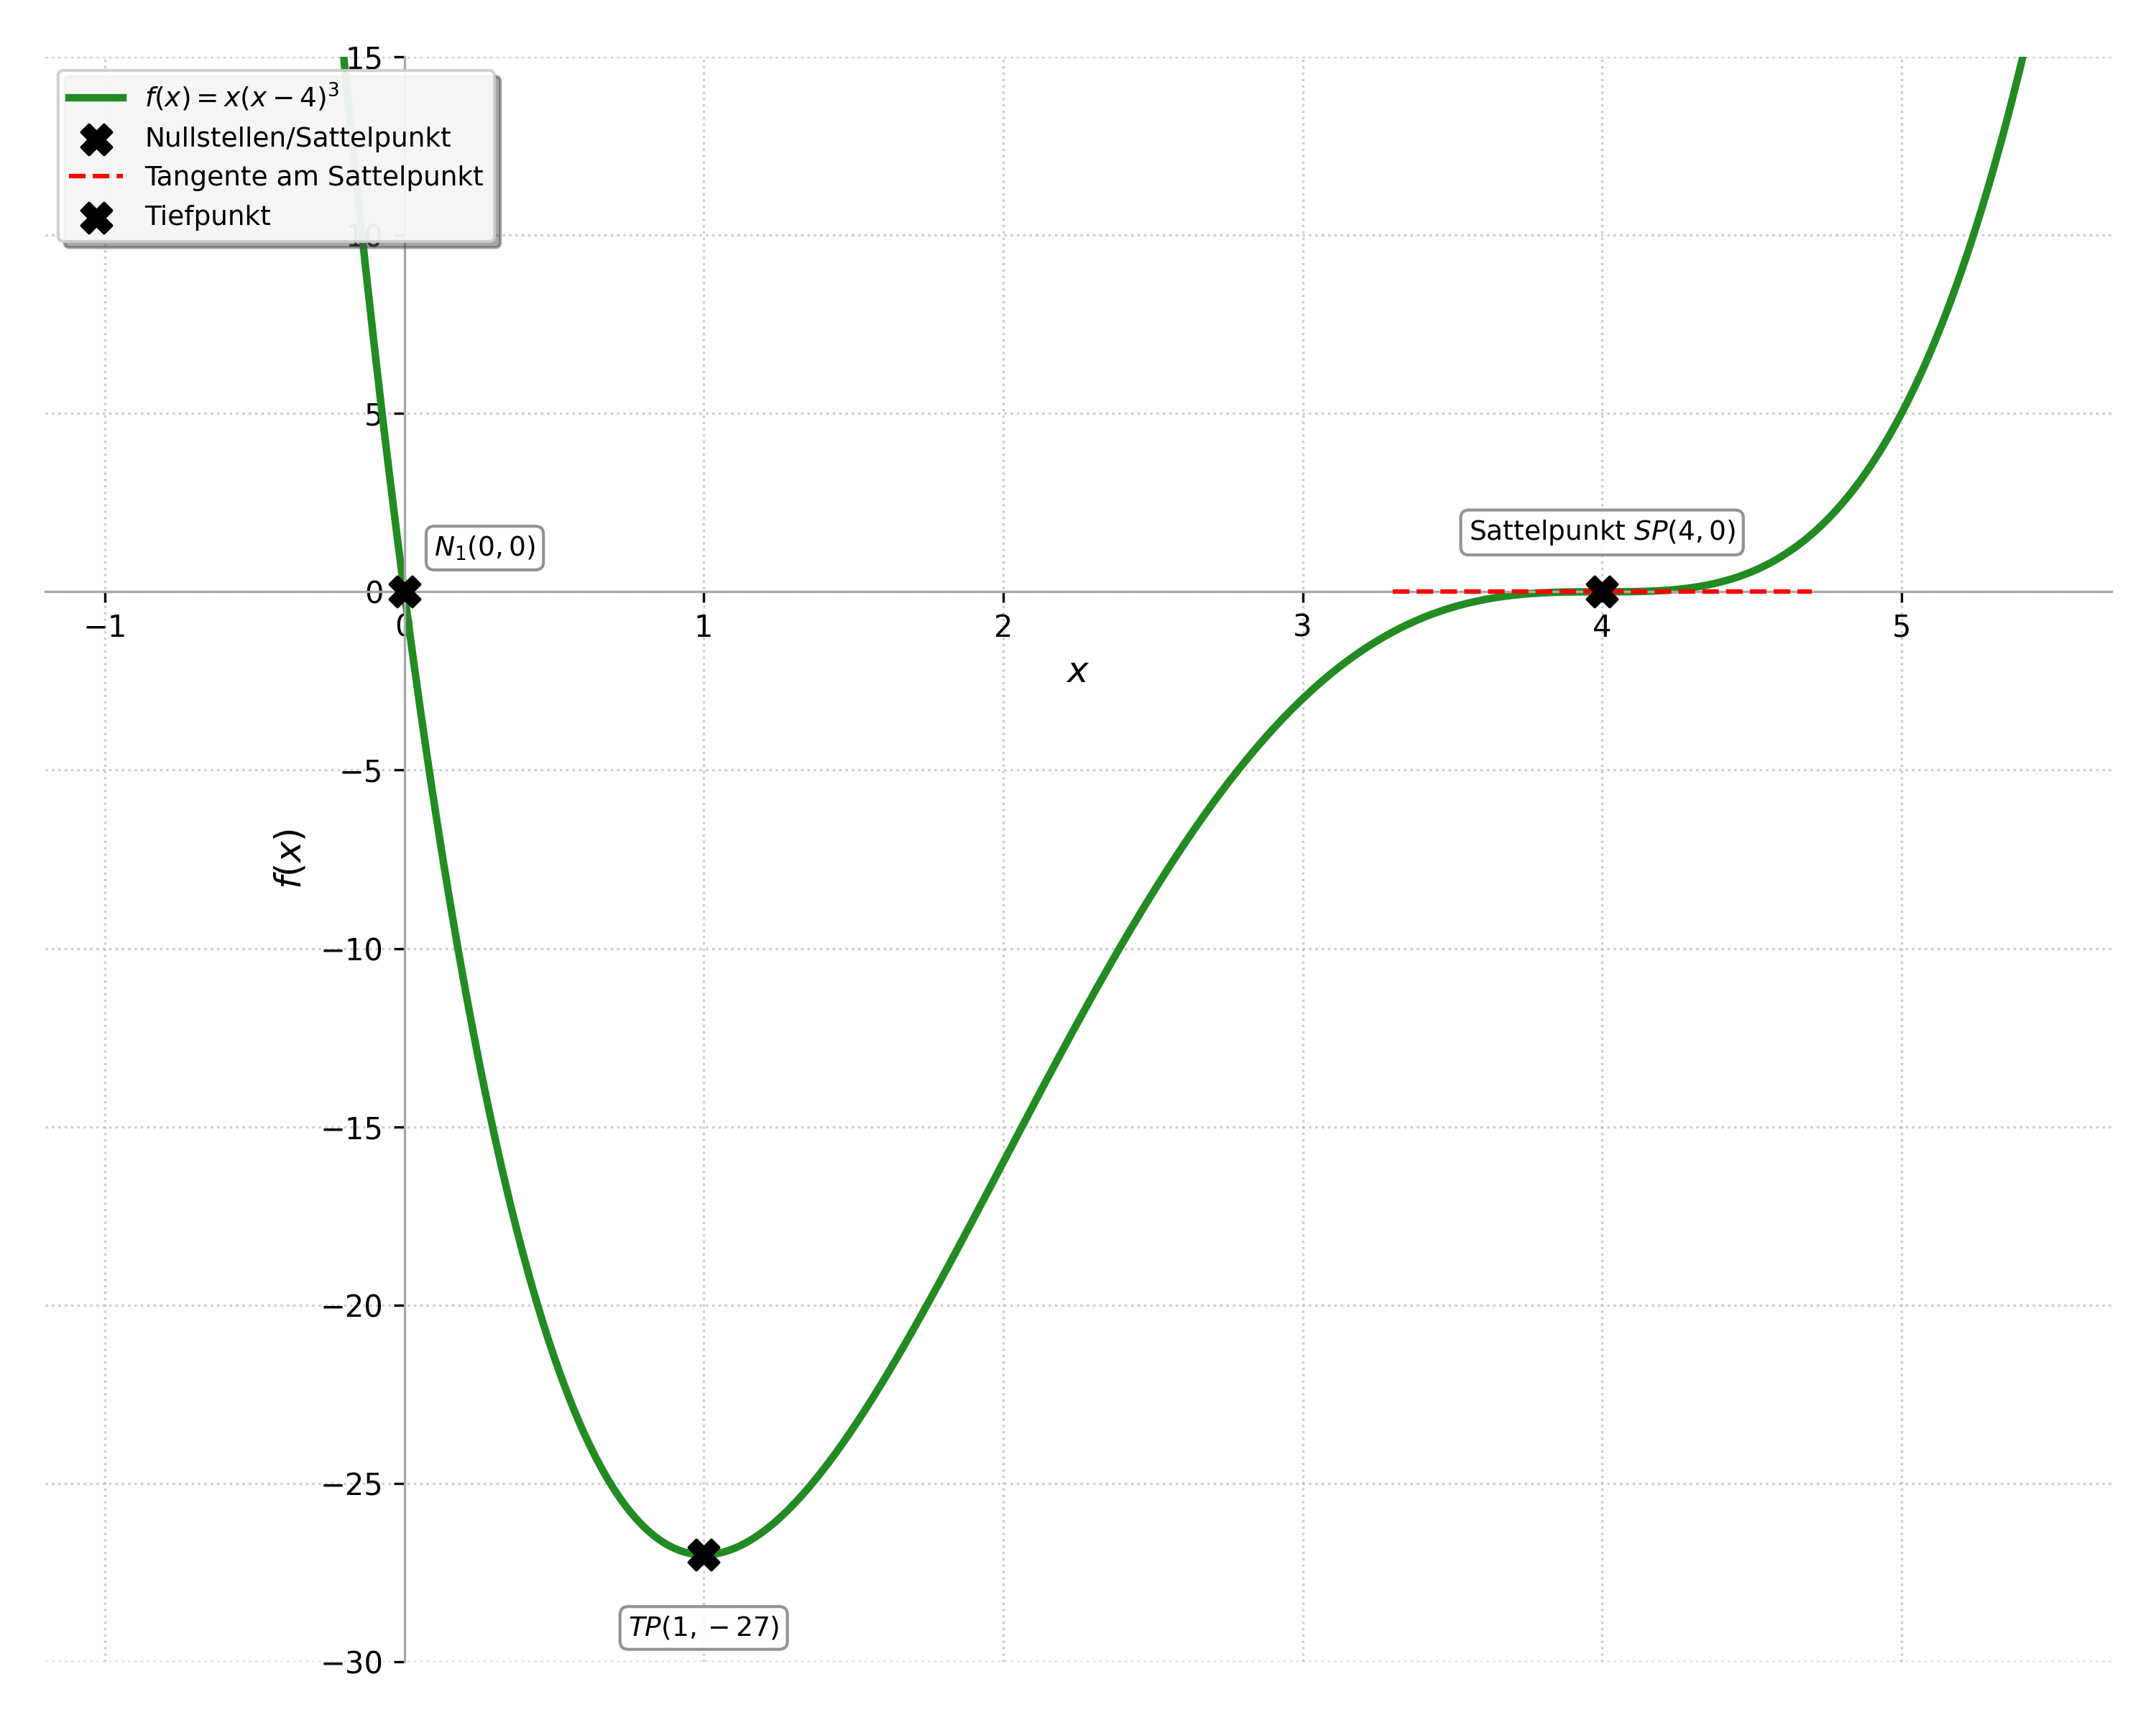
\includegraphics[width=0.8\textwidth]{grafiken/f_tueftler_produkt_kette_graph.png}
        % --- Beschreibung der Skizze ---
        % Die Skizze zeigt den Graphen eines Polynoms 4. Grades.
        % Nullstellen: (0|0) - Schnittpunkt; (4|0) - Sattelpunkt (berührt und durchdringt x-Achse mit horizontaler Tangente).
        % Lokaler Tiefpunkt: (1|-27).
        % Verlauf: Kommt von links oben, fällt zum TP(1|-27), steigt zum SP(4|0), steigt dann weiter nach rechts oben.
        \captionof{figure}{Graph der Funktion $f(x) = x(x-4)^3$.}
        \label{fig:f_tueftler_produkt_kette_graph}
        \end{center}
    \end{itemize}
\end{enumerate}

\end{loesungsumgebung}

\begin{aufgabenumgebung}{Optimierungsproblem – Die optimale Schachtel}
Aus einem quadratischen Stück Pappe der Seitenlänge $L=30\,$cm soll durch Ausschneiden von Quadraten an den Ecken und anschließendes Hochbiegen der entstehenden Seitenlaschen eine offene Schachtel (ohne Deckel) mit maximalem Volumen hergestellt werden.


\begin{enumerate}
    \item \textbf{Variable festlegen:} Sei $x$ die Seitenlänge der Quadrate, die an den Ecken ausgeschnitten werden.
    \item \textbf{Maße der Schachtel:} Drücke die Länge $l$, die Breite $b$ und die Höhe $h$ der entstehenden Schachtel in Abhängigkeit von $x$ aus. Bedenke, dass von jeder Seite der Pappe $2x$ weggeschnitten wird.
    \item \textbf{Definitionsbereich für $x$:} Welche Werte für $x$ sind in diesem Sachzusammenhang sinnvoll? (Die Seitenlängen müssen positiv sein, und man kann nicht mehr wegschneiden, als Pappe da ist).
    \item \textbf{Zielfunktion für das Volumen:} Stelle die Funktion $V(x)$ auf, die das Volumen der Schachtel in Abhängigkeit von $x$ beschreibt ($V = l \cdot b \cdot h$).
    \item \textbf{Extremwertsuche:}
        \begin{itemize}
            \item Bilde die erste Ableitung $V'(x)$.
            \item Setze $V'(x)=0$ und löse nach $x$, um die kritischen Stellen zu finden.
            \item Überprüfe mit der zweiten Ableitung $V''(x)$ (oder dem Vorzeichenwechselkriterium von $V'(x)$), ob an den kritischen Stellen ein Maximum oder Minimum vorliegt.
            \item Berücksichtige den Definitionsbereich von $x$: Liegen die gefundenen Extremstellen im sinnvollen Bereich?
        \end{itemize}
    \item \textbf{Antwort:} Gib die Seitenlänge $x$ der auszuschneidenden Quadrate an, für die das Volumen der Schachtel maximal wird, sowie das maximale Volumen selbst.
\end{enumerate}
\end{aufgabenumgebung}

\begin{loesungsumgebung}[loes:optimierung-schachtel]{Optimierungsproblem – Die optimale Schachtel}

\begin{enumerate}
    \item \textbf{Variable festlegen:}
    Sei $x$ die Seitenlänge der Quadrate (in cm), die an den Ecken des quadratischen Stücks Pappe ausgeschnitten werden. Diese Seitenlänge $x$ wird dann auch die Höhe der entstehenden Schachtel sein.

    \item \textbf{Maße der Schachtel:}
    Die ursprüngliche Pappe hat eine Seitenlänge von $L=30\,$cm. Wenn an jeder Ecke ein Quadrat der Seitenlänge $x$ ausgeschnitten wird, verringert sich jede Seite der entstehenden Grundfläche um $2x$.
    \begin{itemize}
        \item Höhe der Schachtel: $h = x$.
        \item Länge der Grundfläche: $l = L - 2x = 30 - 2x$.
        \item Breite der Grundfläche: $b = L - 2x = 30 - 2x$.
    \end{itemize}

    \item \textbf{Definitionsbereich für $x$:}
    Damit eine Schachtel entstehen kann, muss $x$ positiv sein: $x > 0$.
    Außerdem müssen die Seitenlängen der Grundfläche positiv sein: $30 - 2x > 0$.
    $30 > 2x \Rightarrow 15 > x$.
    Zusammenfassend muss $0 < x < 15$ gelten. Der sinnvolle Definitionsbereich für $x$ ist also das offene Intervall $\mathbf{(0, 15)}$ cm.

    \item \textbf{Zielfunktion für das Volumen:}
    Das Volumen $V$ einer Schachtel ist $V = l \cdot b \cdot h$.
    $V(x) = (30-2x) \cdot (30-2x) \cdot x = (30-2x)^2 x$.
    Ausmultipliziert ergibt sich:
    $V(x) = (900 - 120x + 4x^2)x = \mathbf{4x^3 - 120x^2 + 900x}$.

    \item \textbf{Extremwertsuche:}
    \begin{itemize}
        \item \textbf{Erste Ableitung $V'(x)$ bilden:}
        $V'(x) = \frac{d}{dx}(4x^3 - 120x^2 + 900x) = 12x^2 - 240x + 900$.
        \item \textbf{Kritische Stellen finden ($V'(x)=0$):}
        $12x^2 - 240x + 900 = 0$.
        Wir teilen die Gleichung durch 12:
        $x^2 - 20x + 75 = 0$.
        Mit der p-q-Formel ($p=-20, q=75$):
        $x_{1,2} = - \frac{-20}{2} \pm \sqrt{\left(\frac{-20}{2}\right)^2 - 75}$
        $x_{1,2} = 10 \pm \sqrt{(-10)^2 - 75}$
        $x_{1,2} = 10 \pm \sqrt{100 - 75}$
        $x_{1,2} = 10 \pm \sqrt{25}$
        $x_{1,2} = 10 \pm 5$.
        Die kritischen Stellen sind $x_1 = 10 + 5 = 15$ und $x_2 = 10 - 5 = 5$.
        \item \textbf{Überprüfung mit der zweiten Ableitung $V''(x)$:}
        $V''(x) = \frac{d}{dx}(12x^2 - 240x + 900) = 24x - 240$.
        Für $x_1 = 15$: $V''(15) = 24(15) - 240 = 360 - 240 = 120$.
        Da $V''(15) > 0$, liegt bei $x=15$ ein lokales Minimum vor.
        Für $x_2 = 5$: $V''(5) = 24(5) - 240 = 120 - 240 = -120$.
        Da $V''(5) < 0$, liegt bei $x=5$ ein lokales Maximum vor.
        \item \textbf{Berücksichtigung des Definitionsbereichs von $x$:}
        Der Definitionsbereich ist $(0, 15)$.
        Die kritische Stelle $x_1=15$ liegt nicht im offenen Definitionsbereich (hier wäre die Grundfläche Null).
        Die kritische Stelle $x_2=5$ liegt im Definitionsbereich $(0,15)$. Da es sich um ein lokales Maximum handelt und an den Rändern des Definitionsbereichs das Volumen gegen Null geht ($V(x) \to 0$ für $x \to 0^+$ und $V(x) = 0$ für $x=15$), ist dies das globale Maximum im sinnvollen Bereich.
    \end{itemize}

    \item \textbf{Antwort:}
    Die Seitenlänge $x$ der auszuschneidenden Quadrate, für die das Volumen der Schachtel maximal wird, ist $\mathbf{x = 5\,cm}$.
    Das maximale Volumen beträgt:
    $V(5) = (30-2(5))^2 \cdot 5 = (30-10)^2 \cdot 5 = (20)^2 \cdot 5 = 400 \cdot 5 = \mathbf{2000\,cm^3}$.
    Die Abmessungen der Schachtel mit maximalem Volumen sind:
    \begin{itemize}
        \item Höhe: $h = x = 5\,$cm.
        \item Länge der Grundfläche: $l = 30 - 2(5) = 20\,$cm.
        \item Breite der Grundfläche: $b = 30 - 2(5) = 20\,$cm.
    \end{itemize}
\end{enumerate}

\end{loesungsumgebung}

\begin{aufgabenumgebung}{Rekonstruktion einer Polynomfunktion}
Eine ganzrationale Funktion dritten Grades $f(x) = ax^3 + bx^2 + cx + d$ hat die folgenden Eigenschaften:
\begin{itemize}
    \item Der Graph der Funktion geht durch den Ursprung $P(0|0)$.
    \item Der Ursprung ist gleichzeitig ein Wendepunkt der Funktion.
    \item Die Tangente im Wendepunkt (die Wendetangente) hat die Gleichung $y_W(x) = -3x$.
    \item Der Graph der Funktion hat eine Nullstelle bei $x_N = 1$.
\end{itemize}
Bestimme die Funktionsgleichung $f(x)$.



\end{aufgabenumgebung}


\begin{loesungsumgebung}[loes:rekonstruktion-polynom3]{Rekonstruktion einer Polynomfunktion}
Die allgemeine Form der gesuchten ganzrationalen Funktion dritten Grades ist $f(x) = ax^3 + bx^2 + cx + d$.
Ihre Ableitungen lauten:
$f'(x) = 3ax^2 + 2bx + c$
$f''(x) = 6ax + 2b$

Wir übersetzen die gegebenen Eigenschaften in Gleichungen:

\begin{itemize}
    \item \textbf{Der Graph der Funktion geht durch den Ursprung $P(0|0)$:} \\
    Diese Bedingung bedeutet $f(0)=0$.
    $f(0) = a(0)^3 + b(0)^2 + c(0) + d = 0 \Rightarrow \mathbf{d=0}$. (Gleichung 1)

    \item \textbf{Der Ursprung ist gleichzeitig ein Wendepunkt der Funktion:} \\
    Ein Wendepunkt liegt an der Stelle $x_W=0$. Notwendige Bedingung für einen Wendepunkt ist $f''(x_W)=0$.
    $f''(0) = 6a(0) + 2b = 0 \Rightarrow 2b=0 \Rightarrow \mathbf{b=0}$. (Gleichung 2)
    (Hinweis: Damit es tatsächlich ein Wendepunkt ist, müsste $f'''(0) \neq 0$ sein. $f'''(x)=6a$. Wenn $a \neq 0$, ist diese Bedingung erfüllt.)

    \item \textbf{Die Tangente im Wendepunkt (Ursprung) hat die Gleichung $y_W(x) = -3x$:} \\
    Der Wendepunkt ist $W(0|0)$. Die Steigung der Wendetangente ist die Ableitung $f'(x_W)$ an der Wendestelle $x_W=0$. Die gegebene Tangentengleichung $y_W(x)=-3x$ hat die Steigung $m_W=-3$.
    Also $f'(0) = -3$.
    $f'(0) = 3a(0)^2 + 2b(0) + c = -3 \Rightarrow \mathbf{c=-3}$. (Gleichung 3)

    \item \textbf{Der Graph der Funktion hat eine Nullstelle bei $x_N = 1$:} \\
    Diese Bedingung bedeutet $f(1)=0$.
    $f(1) = a(1)^3 + b(1)^2 + c(1) + d = 0 \Rightarrow a+b+c+d=0$. (Gleichung 4)
\end{itemize}

\textbf{Lösen des Gleichungssystems:}
Wir haben bereits direkt erhalten:
\begin{itemize}
    \item $d=0$ (aus Gleichung 1)
    \item $b=0$ (aus Gleichung 2)
    \item $c=-3$ (aus Gleichung 3)
\end{itemize}
Diese Werte setzen wir in Gleichung 4 ein:
$a + b + c + d = 0$
$a + 0 + (-3) + 0 = 0$
$a - 3 = 0 \Rightarrow \mathbf{a=3}$.

Die Koeffizienten der Funktion sind also $a=3, b=0, c=-3, d=0$.

\textbf{Funktionsgleichung:}
Die gesuchte Funktionsgleichung lautet:
$f(x) = 3x^3 + 0x^2 - 3x + 0$
$$ \mathbf{f(x) = 3x^3 - 3x} $$

\textbf{Überprüfung (optional):}
\begin{itemize}
    \item $f(0) = 3(0)^3 - 3(0) = 0$. (Punkt $P(0|0)$ liegt auf dem Graphen)
    \item $f'(x) = 9x^2 - 3$, $f''(x) = 18x$, $f'''(x) = 18$.
    \item $f''(0) = 18(0) = 0$. $f'''(0) = 18 \neq 0$. Also ist bei $x=0$ ein Wendepunkt.
    \item $f'(0) = 9(0)^2 - 3 = -3$. Die Steigung der Wendetangente im Ursprung ist $-3$, die Tangente ist $y=-3x$.
    \item $f(1) = 3(1)^3 - 3(1) = 3-3=0$. (Nullstelle bei $x=1$)
\end{itemize}
Alle Bedingungen sind erfüllt.
\end{loesungsumgebung}


\begin{aufgabenumgebung}{Bewegungsanalyse – Zwei Läufer auf der Bahn}
Zwei Läufer, A und B, bewegen sich auf einer geraden Bahn.
Läufer A startet zum Zeitpunkt $t=0\,$s am Punkt $s_A(0)=0\,$m. Seine Position (in Metern) zum Zeitpunkt $t$ (in Sekunden) wird durch die Funktion $s_A(t) = t^2$ beschrieben.
Läufer B startet gleichzeitig am Punkt $s_B(0)=10\,$m. Seine Position wird durch $s_B(t) = -0.5t^2 + 7t + 10$ beschrieben.
Wir betrachten das Zeitintervall $[0, 5]$ Sekunden.

\begin{enumerate}
    \item \textbf{Geschwindigkeiten:} Bestimme die Geschwindigkeitsfunktionen $v_A(t) = s_A'(t)$ und $v_B(t) = s_B'(t)$ der beiden Läufer.
    \item \textbf{Gleiche Geschwindigkeit:} Zu welchem Zeitpunkt $t$ haben beide Läufer die gleiche Geschwindigkeit? Wie groß ist diese Geschwindigkeit?
    \item \textbf{Gleiche Position:} Haben die Läufer jemals die gleiche Position im betrachteten Zeitintervall $[0,5]$? Wenn ja, zu welchem Zeitpunkt/welchen Zeitpunkten?
    \item \textbf{Abstand der Läufer:}
        \begin{itemize}
            \item Stelle eine Funktion $d(t)$ auf, die den Abstand zwischen den beiden Läufern zum Zeitpunkt $t$ beschreibt. 
            \textit{Hinweis:} Überlege zuerst, welcher Läufer im Intervall $[0,5]$ vorne liegt, um das Betragszeichen bei der Differenz $d(t) = |s_B(t) - s_A(t)|$ auflösen zu können. Du hast in Teil c) untersucht, ob sie sich treffen.
            \item Zu welchem Zeitpunkt im Intervall $[0,5]$ ist der Abstand zwischen den Läufern minimal? Wie groß ist dieser minimale Abstand?
            \item Zu welchem Zeitpunkt im Intervall $[0,5]$ ist der Abstand zwischen den Läufern maximal? Wie groß ist dieser maximale Abstand?
        \end{itemize}
\end{enumerate}
\end{aufgabenumgebung}


\begin{loesungsumgebung}[loes:bewegung-zwei-laeufer]{Bewegungsanalyse – Zwei Läufer auf der Bahn}
Wir analysieren die Bewegung der Läufer A und B im Zeitintervall $[0, 5]$ Sekunden.
Die Positionen sind gegeben durch $s_A(t) = t^2$ und $s_B(t) = -0.5t^2 + 7t + 10$.

\begin{enumerate}[label=(\alph*)]
    \item \textbf{Geschwindigkeiten:}
    Die Geschwindigkeitsfunktionen sind die ersten Ableitungen der Ortsfunktionen:
    \begin{itemize}
        \item Für Läufer A: $v_A(t) = s_A'(t) = \frac{d}{dt}(t^2) = \mathbf{2t}$ (m/s).
        \item Für Läufer B: $v_B(t) = s_B'(t) = \frac{d}{dt}(-0.5t^2 + 7t + 10) = -0.5 \cdot 2t + 7 = \mathbf{-t + 7}$ (m/s).
    \end{itemize}

    \item \textbf{Gleiche Geschwindigkeit:}
    Wir setzen $v_A(t) = v_B(t)$:
    $2t = -t + 7$
    $$
    \begin{array}{r c l c l}
    \umformung{2t}{-t+7}{+}{t}
    \umformung{3t}{7}{\div}{3}
    \umformungend{t}{7/3}
    \end{array}
    $$
    Zum Zeitpunkt $\mathbf{t = \frac{7}{3}\,s \approx 2.33\,s}$ haben beide Läufer die gleiche Geschwindigkeit.
    Diese Geschwindigkeit beträgt:
    $v_A(\frac{7}{3}) = 2 \cdot \frac{7}{3} = \frac{14}{3}\,$m/s.
    $v_B(\frac{7}{3}) = -\frac{7}{3} + 7 = -\frac{7}{3} + \frac{21}{3} = \frac{14}{3}\,$m/s.
    Die gemeinsame Geschwindigkeit ist $\mathbf{\frac{14}{3}\,m/s \approx 4.67\,m/s}$.

    \item \textbf{Gleiche Position:}
    Wir setzen $s_A(t) = s_B(t)$:
    $t^2 = -0.5t^2 + 7t + 10$
    $1.5t^2 - 7t - 10 = 0$.
    Multiplikation mit 2 ergibt: $3t^2 - 14t - 20 = 0$.
    Wir verwenden die Mitternachtsformel $t_{1,2} = \frac{-b \pm \sqrt{b^2-4ac}}{2a}$ mit $a=3, b=-14, c=-20$:
    $D = (-14)^2 - 4(3)(-20) = 196 + 240 = 436$.
    $t_{1,2} = \frac{14 \pm \sqrt{436}}{2 \cdot 3} = \frac{14 \pm 2\sqrt{109}}{6} = \frac{7 \pm \sqrt{109}}{3}$.
    $t_1 = \frac{7 + \sqrt{109}}{3} \approx \frac{7 + 10.440}{3} \approx \frac{17.440}{3} \approx 5.813\,$s.
    $t_2 = \frac{7 - \sqrt{109}}{3} \approx \frac{7 - 10.440}{3} \approx \frac{-3.440}{3} \approx -1.147\,$s.
    Der Zeitpunkt $t_1 \approx 5.813\,$s liegt außerhalb des Intervalls $[0,5]$. Der Zeitpunkt $t_2 \approx -1.147\,$s ist negativ und somit nicht relevant.
    Daher haben die Läufer im betrachteten Zeitintervall $[0,5]$ \textbf{niemals die gleiche Position}.

    \item \textbf{Abstand der Läufer:}
    \begin{itemize}
        \item \textbf{Abstandsfunktion $d(t)$:}
        Da sich die Läufer im Intervall $[0,5]$ nicht treffen und $s_A(0)=0$ sowie $s_B(0)=10$ ist ($s_B(0) > s_A(0)$), liegt Läufer B im gesamten Intervall $[0,5]$ vor Läufer A.
        Somit ist der Abstand $d(t) = s_B(t) - s_A(t)$.
        $d(t) = (-0.5t^2 + 7t + 10) - (t^2) = \mathbf{-1.5t^2 + 7t + 10}$.

        \item \textbf{Minimaler Abstand im Intervall $[0,5]$:}
        Um den minimalen Abstand zu finden, untersuchen wir die Extremwerte von $d(t)$ im Intervall $[0,5]$.
        $d'(t) = \frac{d}{dt}(-1.5t^2 + 7t + 10) = -3t + 7$.
        Kritische Stelle: $d'(t)=0 \Rightarrow -3t + 7 = 0 \Rightarrow 3t=7 \Rightarrow t = \frac{7}{3}$.
        $t = \frac{7}{3} \approx 2.33\,$s liegt im Intervall $[0,5]$.
        Zweite Ableitung: $d''(t) = -3$.
        Da $d''(\frac{7}{3}) = -3 < 0$, liegt bei $t=\frac{7}{3}\,$s ein lokales Maximum des Abstands vor.
        Der minimale Abstand muss also an den Rändern des Intervalls $[0,5]$ angenommen werden.
        $d(0) = -1.5(0)^2 + 7(0) + 10 = 10\,$m.
        $d(5) = -1.5(5)^2 + 7(5) + 10 = -1.5(25) + 35 + 10 = -37.5 + 35 + 10 = 7.5\,$m.
        Der minimale Abstand beträgt $\mathbf{7.5\,m}$ zum Zeitpunkt $\mathbf{t=5\,s}$.

        \item \textbf{Maximaler Abstand im Intervall $[0,5]$:}
        Wir vergleichen die Werte an den Rändern und am lokalen Extremum (welches hier ein Maximum ist):
        $d(0) = 10\,$m.
        $d(5) = 7.5\,$m.
        $d(\frac{7}{3}) = -1.5\left(\frac{7}{3}\right)^2 + 7\left(\frac{7}{3}\right) + 10 = -1.5\left(\frac{49}{9}\right) + \frac{49}{3} + 10$
        $d(\frac{7}{3}) = -\frac{3}{2} \cdot \frac{49}{9} + \frac{49}{3} + 10 = -\frac{49}{6} + \frac{98}{6} + \frac{60}{6} = \frac{-49+98+60}{6} = \frac{109}{6}$.
        $d(\frac{7}{3}) = \frac{109}{6} \approx 18.167\,$m.
        Der maximale Abstand beträgt $\mathbf{\frac{109}{6}\,m \approx 18.17\,m}$ zum Zeitpunkt $\mathbf{t=\frac{7}{3}\,s}$.
    \end{itemize}
\end{enumerate}

\end{loesungsumgebung}


\begin{aufgabenumgebung}{Tangentenprobleme an einer kubischen Funktion}
Gegeben ist die Funktion $f(x) = x^3 - 3x$.
\begin{enumerate}
    \item \textbf{Parallele Tangenten:}
        \begin{itemize}
            \item Bestimme die Steigung der Geraden $g(x) = 9x - 5$.
            \item Gibt es Punkte auf dem Graphen von $f(x)$, an denen die Tangente parallel zur Geraden $g(x)$ ist? Wenn ja, bestimme die Koordinaten dieser Punkte.
            \item Gib die Gleichungen der Tangenten an den Graphen von $f(x)$ in diesen Punkten an.
        \end{itemize}
    \item \textbf{Tangente von einem externen Punkt:}
        Von welchem Punkt $P_y(0|y_P)$ auf der y-Achse aus kann man eine Tangente an den Graphen von $f(x)$ legen, die den Graphen an der Stelle $x_B=2$ berührt?

\end{enumerate}
\end{aufgabenumgebung}

\begin{loesungsumgebung}[loes:tangentenprobleme-kubisch]{Tangentenprobleme an einer kubischen Funktion}
Gegeben ist die Funktion $f(x) = x^3 - 3x$. Ihre erste Ableitung ist $f'(x) = 3x^2 - 3$.

\begin{enumerate}[label=(\alph*)]
    \item \textbf{Parallele Tangenten:}
    \begin{itemize}
        \item \textbf{Steigung der Geraden $g(x) = 9x - 5$:}
        Die Steigung $m_g$ der Geraden $g(x)$ ist der Koeffizient von $x$, also $\mathbf{m_g = 9}$.

        \item \textbf{Punkte auf dem Graphen von $f(x)$, an denen die Tangente parallel zur Geraden $g(x)$ ist:}
        Parallelität bedeutet gleiche Steigung. Wir suchen also Stellen $x$, an denen $f'(x) = m_g = 9$ gilt.
        $3x^2 - 3 = 9$
        $$
        \begin{array}{r c l c l}
        \umformung{3x^2 - 3}{9}{+}{3}
        \umformung{3x^2}{12}{\div}{3}
        \umformungend{x^2}{4}
        \end{array}
        $$
        Aus $x^2=4$ folgt $x = \pm\sqrt{4}$, also $x_1 = 2$ und $x_2 = -2$.
        Dies sind die x-Koordinaten der gesuchten Punkte. Die y-Koordinaten sind:
        $f(2) = (2)^3 - 3(2) = 8 - 6 = 2$. Punkt $\mathbf{P_1(2|2)}$.
        $f(-2) = (-2)^3 - 3(-2) = -8 + 6 = -2$. Punkt $\mathbf{P_2(-2|-2)}$.

        \item \textbf{Gleichungen der Tangenten an den Graphen von $f(x)$ in diesen Punkten:}
        Die Steigung beider Tangenten ist $m_t = 9$.
        \begin{itemize}
            \item Tangente $t_1$ im Punkt $P_1(2|2)$:
            $y - y_1 = m_t(x - x_1)$
            $y - 2 = 9(x - 2)$
            $y = 9x - 18 + 2$
            $\mathbf{t_1(x): y = 9x - 16}$.
            \item Tangente $t_2$ im Punkt $P_2(-2|-2)$:
            $y - y_2 = m_t(x - x_2)$
            $y - (-2) = 9(x - (-2))$
            $y + 2 = 9(x + 2)$
            $y = 9x + 18 - 2$
            $\mathbf{t_2(x): y = 9x + 16}$.
        \end{itemize}
    \end{itemize}

    \item \textbf{Tangente von einem externen Punkt:}
    Gesucht ist der Punkt $P_y(0|y_P)$ auf der y-Achse, von dem aus eine Tangente an $f(x)$ den Graphen an der Stelle $x_B=2$ berührt.
    \begin{enumerate}[label=\arabic*.]
        \item \textbf{Bestimme die y-Koordinate des Berührpunkts $B(2|f(2))$:}
        $f(2) = (2)^3 - 3(2) = 8 - 6 = 2$.
        Der Berührpunkt ist $\mathbf{B(2|2)}$.

        \item \textbf{Bestimme die Steigung $m_T$ der Tangente an $f(x)$ an der Stelle $x_B=2$:}
        $m_T = f'(x_B) = f'(2) = 3(2)^2 - 3 = 3(4) - 3 = 12 - 3 = \mathbf{9}$.

        \item \textbf{Stelle die Gleichung der Tangente $t_B(x)$ im Punkt $B$ auf:}
        Mit dem Punkt $B(2|2)$ und der Steigung $m_T=9$:
        $y - 2 = 9(x - 2)$
        $y = 9x - 18 + 2$
        $\mathbf{t_B(x): y = 9x - 16}$.

        \item \textbf{Der gesuchte Punkt $P_y(0|y_P)$ muss auf dieser Tangente $t_B(x)$ liegen:}
        Setze $x=0$ in die Tangentengleichung $y = 9x - 16$ ein, um $y_P$ zu finden:
        $y_P = 9(0) - 16 = -16$.
        Der gesuchte Punkt auf der y-Achse ist $\mathbf{P_y(0|-16)}$.
    \end{enumerate}
\end{enumerate}

\end{loesungsumgebung}


\begin{aufgabenumgebung}{Checkliste: Von kubischen Funktionen zu linearen Ableitungen}
Diese Aufgabe zeigt dir, wie dein Wissen über lineare Funktionen dir hilft, das Verhalten von Polynomen 3. Grades zu verstehen.
Betrachte die Funktion $f(x) = x^3 - 6x^2 + 10x - 3$.

\begin{enumerate}[label=(\alph*)]
    \item \textbf{Ableitungen bilden:} Berechne die erste Ableitung $f'(x)$ und die zweite Ableitung $f''(x)$ der Funktion $f(x)$.
    \item \textbf{Analyse der zweiten Ableitung:}
    \begin{itemize}
        \item Welchen Funktionstyp erkennst du in $f''(x)$? Gib die Steigung $m_{f''}$ und den y-Achsenabschnitt $c_{f''}$ dieser Funktion an.
        \item Berechne die Nullstelle $x_W$ von $f''(x)$. Welche besondere Bedeutung hat diese Stelle $x_W$ für den Graphen der ursprünglichen Funktion $f(x)$? (Erinnere dich an die Definition von Wendepunkten).
    \end{itemize}
    \item \textbf{Krümmungsverhalten von $f(x)$ bestimmen:}
    Nutze dein Wissen über lineare Funktionen, um das Vorzeichen von $f''(x)$ zu bestimmen:
    \begin{itemize}
        \item Für welche $x$-Werte ist $f''(x) > 0$? (Tipp: Wann sind die Werte einer steigenden/fallenden linearen Funktion positiv?)
        \item Für welche $x$-Werte ist $f''(x) < 0$?
        \item Welche Schlussfolgerungen ziehst du daraus für das Krümmungsverhalten (links- oder rechtsgekrümmt) des Graphen von $f(x)$? Gib die Intervalle an.
    \end{itemize}
    \item \textbf{Reflexion:} Erkläre in eigenen Worten, warum das Verständnis der Eigenschaften einer linearen Funktion (insbesondere ihrer Nullstelle und des Vorzeichenverlaufs in Abhängigkeit von der Steigung) nützlich ist, um das Krümmungsverhalten einer kubischen Funktion zu analysieren.
\end{enumerate}
\end{aufgabenumgebung}


\begin{loesungsumgebung}[loes:kubisch-zu-linear-ableitung]{Checkliste: Von kubischen Funktionen zu linearen Ableitungen}
Wir betrachten die Funktion $f(x) = x^3 - 6x^2 + 10x - 3$.

\begin{enumerate}[label=(\alph*)]
    \item \textbf{Ableitungen bilden:}
    \begin{itemize}
        \item Erste Ableitung $f'(x)$:
        $$ f'(x) = \frac{d}{dx}(x^3 - 6x^2 + 10x - 3) = \mathbf{3x^2 - 12x + 10} $$
        \item Zweite Ableitung $f''(x)$:
        $$ f''(x) = \frac{d}{dx}(3x^2 - 12x + 10) = \mathbf{6x - 12} $$
    \end{itemize}

    \item \textbf{Analyse der zweiten Ableitung $f''(x) = 6x - 12$:}
    \begin{itemize}
        \item \textbf{Funktionstyp, Steigung und y-Achsenabschnitt:}
        $f''(x)$ ist eine \textbf{lineare Funktion}.
        Ihre Steigung ist $m_{f''} = 6$.
        Ihr y-Achsenabschnitt ist $c_{f''} = -12$ (denn $f''(0) = -12$).
        \item \textbf{Nullstelle $x_W$ von $f''(x)$ und ihre Bedeutung:}
        Wir setzen $f''(x_W) = 0$:
        $6x_W - 12 = 0$
        $6x_W = 12$
        $x_W = 2$.
        Die Nullstelle der zweiten Ableitung ist $\mathbf{x_W = 2}$.
        Diese Stelle $x_W$ ist eine \textbf{potentielle Wendestelle} für die ursprüngliche Funktion $f(x)$. Um dies zu bestätigen, prüfen wir die dritte Ableitung:
        $f'''(x) = \frac{d}{dx}(6x - 12) = 6$.
        Da $f'''(2) = 6 \neq 0$, liegt bei $x_W=2$ tatsächlich ein Wendepunkt von $f(x)$ vor.
    \end{itemize}

    \item \textbf{Krümmungsverhalten von $f(x)$ bestimmen:}
    Das Krümmungsverhalten von $f(x)$ wird durch das Vorzeichen von $f''(x) = 6x - 12$ bestimmt.
    Da $f''(x)$ eine lineare Funktion mit positiver Steigung ($m_{f''} = 6 > 0$) und einer Nullstelle bei $x_W=2$ ist, gilt:
    \begin{itemize}
        \item \textbf{Für welche $x$-Werte ist $f''(x) > 0$?}
        Eine steigende lineare Funktion ist rechts von ihrer Nullstelle positiv.
        Also ist $f''(x) > 0$ für $\mathbf{x > 2}$.
        \item \textbf{Für welche $x$-Werte ist $f''(x) < 0$?}
        Eine steigende lineare Funktion ist links von ihrer Nullstelle negativ.
        Also ist $f''(x) < 0$ für $\mathbf{x < 2}$.
        \item \textbf{Schlussfolgerungen für das Krümmungsverhalten von $f(x)$:}
        \begin{itemize}
            \item Im Intervall $(-\infty, 2)$ ist $f''(x) < 0$, daher ist der Graph von $f(x)$ hier \textbf{rechtsgekrümmt} (konkav).
            \item Im Intervall $(2, \infty)$ ist $f''(x) > 0$, daher ist der Graph von $f(x)$ hier \textbf{linksgekrümmt} (konvex).
        \end{itemize}
        Bei $x=2$ findet ein Wechsel des Krümmungsverhaltens statt, was den Wendepunkt bestätigt.
    \end{itemize}

    \item \textbf{Reflexion:}
    Die zweite Ableitung $f''(x)$ einer kubischen Funktion $f(x)$ ist stets eine lineare Funktion. Die Analyse dieser linearen Funktion $f''(x)$ ist entscheidend für das Verständnis des Krümmungsverhaltens der kubischen Funktion $f(x)$:
    \begin{itemize}
        \item Die \textbf{Nullstelle $x_W$ der linearen Funktion $f''(x)$} gibt die x-Koordinate des Wendepunkts der kubischen Funktion $f(x)$ an. An dieser Stelle ändert $f(x)$ sein Krümmungsverhalten.
        \item Das \textbf{Vorzeichen der linearen Funktion $f''(x)$} bestimmt die Krümmungsrichtung von $f(x)$:
        \begin{itemize}
            \item Ist $f''(x) > 0$, so ist $f(x)$ linksgekrümmt.
            \item Ist $f''(x) < 0$, so ist $f(x)$ rechtsgekrümmt.
        \end{itemize}
        \item Die \textbf{Steigung der linearen Funktion $f''(x)$} (also der Koeffizient von $x$ in $f''(x)$ bzw. der Wert $f'''(x)$) gibt an, wie sich die Krümmung ändert. Ist die Steigung von $f''(x)$ positiv, so wechselt $f''(x)$ an seiner Nullstelle von negativen zu positiven Werten, was für $f(x)$ einen Übergang von Rechts- zu Linkskrümmung bedeutet. Ist die Steigung von $f''(x)$ negativ, ist es umgekehrt.
    \end{itemize}
    Indem man also die Eigenschaften einer einfachen linearen Funktion (ihre Nullstelle und wie ihr Vorzeichen von der Steigung abhängt) versteht, kann man direkt auf das komplexere Krümmungsverhalten einer kubischen Funktion schließen. Dies vereinfacht die Analyse erheblich.
\end{enumerate}

\end{loesungsumgebung}

\begin{aufgabenumgebung}{Checkliste: Von Polynomen 4. Grades zu quadratischen Ableitungen}
Diese Aufgabe zeigt dir, wie dein Wissen über quadratische Funktionen dir hilft, das Verhalten von Polynomen 4. Grades zu verstehen.
Betrachte die Funktion $g(x) = \frac{1}{4}x^4 - x^3 + x^2 + 1$.

\begin{enumerate}[label=(\alph*)]
    \item \textbf{Ableitungen bilden:} Berechne die erste Ableitung $g'(x)$ und die zweite Ableitung $g''(x)$ der Funktion $g(x)$.
    \item \textbf{Analyse der zweiten Ableitung:}
    \begin{itemize}
        \item Welchen Funktionstyp erkennst du in $g''(x)$? Gib die Parameter dieser Funktion an (z.B. Öffnungsfaktor, etc.). Ist der Graph von $g''(x)$ nach oben oder unten geöffnet?
        \item Berechne die Nullstellen $x_{W1}, x_{W2}$ von $g''(x)$ (falls vorhanden). Welche Bedeutung haben diese Stellen für den Graphen von $g(x)$?
    \end{itemize}
    \item \textbf{Krümmungsverhalten von $g(x)$ bestimmen:}
    Nutze dein Wissen über quadratische Funktionen, um das Vorzeichen von $g''(x)$ zu bestimmen:
    \begin{itemize}
        \item Skizziere (oder stelle dir vor) den Graphen von $g''(x)$ basierend auf Öffnungsrichtung und Nullstellen.
        \item Für welche $x$-Werte ist $g''(x) > 0$?
        \item Für welche $x$-Werte ist $g''(x) < 0$?
        \item Welche Schlussfolgerungen ziehst du daraus für das Krümmungsverhalten des Graphen von $g(x)$? Gib die Intervalle an. Wie viele Wendepunkte hat $g(x)$?
    \end{itemize}
    \item \textbf{Reflexion:} Erkläre, wie das Verständnis der Eigenschaften einer quadratischen Funktion (Öffnung, Nullstellen, Vorzeichenverlauf) hilft, das Krümmungsverhalten eines Polynoms 4. Grades zu analysieren.
\end{enumerate}
\end{aufgabenumgebung}


\begin{loesungsumgebung}[loes:polynom4-zu-quadrat-ableitung]{Checkliste: Von Polynomen 4. Grades zu quadratischen Ableitungen}
Wir betrachten die Funktion $g(x) = \frac{1}{4}x^4 - x^3 + x^2 + 1$.

\begin{enumerate}[label=(\alph*)]
    \item \textbf{Ableitungen bilden:}
    \begin{itemize}
        \item Erste Ableitung $g'(x)$:
        $$ g'(x) = \frac{d}{dx}\left(\frac{1}{4}x^4 - x^3 + x^2 + 1\right) = \frac{1}{4} \cdot 4x^3 - 3x^2 + 2x + 0 = \mathbf{x^3 - 3x^2 + 2x} $$
        \item Zweite Ableitung $g''(x)$:
        $$ g''(x) = \frac{d}{dx}(x^3 - 3x^2 + 2x) = \mathbf{3x^2 - 6x + 2} $$
    \end{itemize}

    \item \textbf{Analyse der zweiten Ableitung $g''(x) = 3x^2 - 6x + 2$:}
    \begin{itemize}
        \item \textbf{Funktionstyp, Parameter und Öffnung:}
        $g''(x)$ ist eine \textbf{quadratische Funktion}.
        Die Parameter in der Form $ax^2+bx+c$ sind $a_{g''} = 3$, $b_{g''} = -6$, $c_{g''} = 2$.
        Da der Öffnungsfaktor $a_{g''} = 3 > 0$ ist, ist der Graph von $g''(x)$ eine \textbf{nach oben geöffnete Parabel}.
        \item \textbf{Nullstellen $x_{W1}, x_{W2}$ von $g''(x)$ und ihre Bedeutung:}
        Wir setzen $g''(x_W) = 0$: $3x_W^2 - 6x_W + 2 = 0$.
        Mit der Mitternachtsformel (ABC-Formel):
        $x_W = \frac{-(-6) \pm \sqrt{(-6)^2 - 4(3)(2)}}{2(3)} = \frac{6 \pm \sqrt{36 - 24}}{6} = \frac{6 \pm \sqrt{12}}{6}$.
        Da $\sqrt{12} = \sqrt{4 \cdot 3} = 2\sqrt{3}$, erhalten wir:
        $x_W = \frac{6 \pm 2\sqrt{3}}{6} = 1 \pm \frac{2\sqrt{3}}{6} = 1 \pm \frac{\sqrt{3}}{3}$.
        Die potentiellen Wendestellen sind $\mathbf{x_{W1} = 1 - \frac{\sqrt{3}}{3} \approx 0.423}$ und $\mathbf{x_{W2} = 1 + \frac{\sqrt{3}}{3} \approx 1.577}$.
        Diese Stellen sind Kandidaten für Wendepunkte des Graphen der ursprünglichen Funktion $g(x)$.
        Um dies zu bestätigen, bilden wir $g'''(x) = \frac{d}{dx}(3x^2 - 6x + 2) = 6x - 6$.
        Für $x_{W1} = 1 - \frac{\sqrt{3}}{3}$: $g'''(1 - \frac{\sqrt{3}}{3}) = 6(1 - \frac{\sqrt{3}}{3}) - 6 = 6 - 2\sqrt{3} - 6 = -2\sqrt{3} \neq 0$.
        Für $x_{W2} = 1 + \frac{\sqrt{3}}{3}$: $g'''(1 + \frac{\sqrt{3}}{3}) = 6(1 + \frac{\sqrt{3}}{3}) - 6 = 6 + 2\sqrt{3} - 6 = 2\sqrt{3} \neq 0$.
        Da $g'''(x_W) \neq 0$ an beiden Stellen, sind dies tatsächlich Wendestellen von $g(x)$.
    \end{itemize}

    \item \textbf{Krümmungsverhalten von $g(x)$ bestimmen:}
    Das Krümmungsverhalten von $g(x)$ wird durch das Vorzeichen von $g''(x) = 3x^2 - 6x + 2$ bestimmt.
    \begin{itemize}
        \item \textbf{Skizze/Vorstellung des Graphen von $g''(x)$:}
        Der Graph von $g''(x)$ ist eine nach oben geöffnete Parabel, die die x-Achse an den Stellen $x_{W1} = 1 - \frac{\sqrt{3}}{3}$ und $x_{W2} = 1 + \frac{\sqrt{3}}{3}$ schneidet.
        \item \textbf{Für welche $x$-Werte ist $g''(x) > 0$?}
        Eine nach oben geöffnete Parabel ist außerhalb ihrer Nullstellen positiv.
        Also ist $g''(x) > 0$ für $\mathbf{x < 1 - \frac{\sqrt{3}}{3}}$ oder $\mathbf{x > 1 + \frac{\sqrt{3}}{3}}$.
        \item \textbf{Für welche $x$-Werte ist $g''(x) < 0$?}
        Eine nach oben geöffnete Parabel ist zwischen ihren Nullstellen negativ.
        Also ist $g''(x) < 0$ für $\mathbf{1 - \frac{\sqrt{3}}{3} < x < 1 + \frac{\sqrt{3}}{3}}$.
        \item \textbf{Schlussfolgerungen für das Krümmungsverhalten von $g(x)$ und Anzahl Wendepunkte:}
        \begin{itemize}
            \item Im Intervall $(-\infty, 1 - \frac{\sqrt{3}}{3})$ ist $g''(x) > 0 \Rightarrow g(x)$ ist \textbf{linksgekrümmt (konvex)}.
            \item Im Intervall $(1 - \frac{\sqrt{3}}{3}, 1 + \frac{\sqrt{3}}{3})$ ist $g''(x) < 0 \Rightarrow g(x)$ ist \textbf{rechtsgekrümmt (konkav)}.
            \item Im Intervall $(1 + \frac{\sqrt{3}}{3}, \infty)$ ist $g''(x) > 0 \Rightarrow g(x)$ ist \textbf{linksgekrümmt (konvex)}.
        \end{itemize}
        Da das Krümmungsverhalten an $x_{W1}$ und $x_{W2}$ wechselt, hat die Funktion $g(x)$ genau \textbf{zwei Wendepunkte}.
    \end{itemize}

    \item \textbf{Reflexion:}
    Die zweite Ableitung $g''(x)$ eines Polynoms 4. Grades $g(x)$ ist eine quadratische Funktion. Das Verständnis der Eigenschaften dieser quadratischen Funktion $g''(x)$ ist sehr hilfreich für die Analyse des Krümmungsverhaltens von $g(x)$:
    \begin{itemize}
        \item Die \textbf{Öffnungsrichtung der Parabel $g''(x)$} gibt Aufschluss über die Abfolge der Krümmungsintervalle. Ist $g''(x)$ nach oben geöffnet (wie hier), erwartet man typischerweise eine Abfolge von links- zu rechts- zu linkskrümmung (oder umgekehrt, wenn $g''(x)$ nach unten geöffnet wäre und Nullstellen hätte).
        \item Die \textbf{Nullstellen der quadratischen Funktion $g''(x)$} sind genau die x-Koordinaten der (potentiellen) Wendepunkte der ursprünglichen Funktion $g(x)$. Die Anzahl der verschiedenen reellen Nullstellen von $g''(x)$ (0, 1 oder 2) bestimmt die maximale Anzahl der Wendepunkte von $g(x)$.
        \item Der \textbf{Vorzeichenverlauf von $g''(x)$} (also wo die Parabel $g''(x)$ oberhalb oder unterhalb der x-Achse liegt) bestimmt direkt die Intervalle, in denen $g(x)$ links- bzw. rechtsgekrümmt ist. Kennt man die Öffnung und die Nullstellen der Parabel $g''(x)$, kann man diese Intervalle leicht bestimmen.
    \end{itemize}
    Somit ermöglicht das Wissen über quadratische Funktionen eine systematische und oft vereinfachte Analyse des Krümmungsverhaltens von Polynomen 4. Grades.
\end{enumerate}

\end{loesungsumgebung}



\begin{aufgabenumgebung}{Checkliste: Die maximale Steigung finden (Anwendung)}
Oft ist nicht nur interessant, wo eine Funktion ihren höchsten oder tiefsten Wert hat, sondern auch, wo sie am stärksten steigt oder fällt. Das führt uns zur Untersuchung der Ableitung selbst.
Ein Unternehmen stellt fest, dass seine Produktionskosten $K(x)$ (in Euro) bei der Herstellung von $x$ Einheiten eines Produkts durch die Funktion $K(x) = \frac{1}{3}x^3 - 10x^2 + 150x + 500$ für $x \in [0, 25]$ beschrieben werden können.
Die \textit{Grenzkosten} geben an, um wie viel die Kosten ungefähr steigen, wenn eine Einheit mehr produziert wird. Mathematisch sind die Grenzkosten die Ableitung der Kostenfunktion, also $K'(x)$.
Das Unternehmen möchte wissen, bei welcher Produktionsmenge $x$ die Grenzkosten $K'(x)$ \textbf{minimal} sind (d.h., wann die Kosten pro zusätzlich produzierter Einheit am geringsten ansteigen).

\begin{enumerate}[label=(\alph*)]
    \item \textbf{Grenzkostenfunktion bestimmen:} Bilde die erste Ableitung $K'(x)$ der Kostenfunktion $K(x)$. Diese Funktion $K'(x)$ beschreibt die Steigung der Kostenfunktion.
    \item \textbf{Ziel verstehen:} Wir suchen das Minimum der Funktion $K'(x)$. Wie findet man normalerweise Minima einer Funktion? (Tipp: Denke an die Ableitung der zu untersuchenden Funktion!)
    \item \textbf{Ableitung der Grenzkostenfunktion bilden:} Bilde die Ableitung von $K'(x)$, also die zweite Ableitung der ursprünglichen Kostenfunktion, $K''(x)$.
    \item \textbf{Kritische Stelle für $K'(x)$ finden:} Setze $K''(x) = 0$ und löse nach $x$. Dies ist die potenzielle Stelle $x_W$, an der die Grenzkosten $K'(x)$ minimal (oder maximal) sein könnten.
    \item \textbf{Art des Extremums von $K'(x)$ prüfen:} Überprüfe mit der nächsten Ableitung, also $K'''(x)$, ob bei $x_W$ tatsächlich ein Minimum für $K'(x)$ vorliegt. (Wenn $K'''(x_W) \neq 0$ und $K''(x_W)=0$, dann ist $x_W$ ein Wendepunkt von $K(x)$ und ein Extremum von $K'(x)$). Alternativ: Untersuche den Vorzeichenwechsel von $K''(x)$ bei $x_W$.
    \item \textbf{Antwort formulieren:} Bei welcher Produktionsmenge $x$ sind die Grenzkosten minimal? Wie hoch sind die minimalen Grenzkosten $K'(x_W)$?
    \item \textbf{Reflexion:} Was für ein besonderer Punkt ist $x_W$ für die ursprüngliche Kostenfunktion $K(x)$? Warum ist es plausibel, dass die Steigung einer Funktion (hier $K(x)$) an einem Wendepunkt maximal oder minimal wird?
\end{enumerate}
\end{aufgabenumgebung}

\begin{loesungsumgebung}[loes:maximale-steigung-anwendung]{Checkliste: Die maximale Steigung finden (Anwendung)}
Gegeben ist die Kostenfunktion $K(x) = \frac{1}{3}x^3 - 10x^2 + 150x + 500$ für $x \in [0, 25]$.

\begin{enumerate}[label=(\alph*)]
    \item \textbf{Grenzkostenfunktion bestimmen:}
    Die Grenzkostenfunktion $K'(x)$ ist die erste Ableitung der Kostenfunktion $K(x)$:
    $$ K'(x) = \frac{d}{dx}\left(\frac{1}{3}x^3 - 10x^2 + 150x + 500\right) $$
    $$ K'(x) = \frac{1}{3} \cdot 3x^2 - 10 \cdot 2x + 150 \cdot 1 + 0 $$
    $$ \mathbf{K'(x) = x^2 - 20x + 150} $$
    Diese Funktion beschreibt die (momentane) Änderungsrate der Kosten, also die Steigung der Kostenfunktion.

    \item \textbf{Ziel verstehen:}
    Wir suchen das Minimum der Grenzkostenfunktion $K'(x)$. Um das Minimum einer Funktion zu finden, bildet man deren Ableitung, setzt diese Null, um kritische Stellen zu finden, und überprüft diese Stellen (z.B. mit der zweiten Ableitung dieser Funktion oder dem Vorzeichenwechselkriterium ihrer ersten Ableitung).
    Die Funktion, deren Minimum wir suchen, ist $M(x) = K'(x)$. Ihre Ableitung ist $M'(x) = (K'(x))' = K''(x)$.

    \item \textbf{Ableitung der Grenzkostenfunktion bilden ($K''(x)$):}
    Dies ist die zweite Ableitung der ursprünglichen Kostenfunktion $K(x)$:
    $$ K''(x) = \frac{d}{dx}(K'(x)) = \frac{d}{dx}(x^2 - 20x + 150) $$
    $$ K''(x) = 2x - 20 + 0 $$
    $$ \mathbf{K''(x) = 2x - 20} $$

    \item \textbf{Kritische Stelle für $K'(x)$ finden:}
    Wir setzen die Ableitung von $K'(x)$, also $K''(x)$, gleich Null:
    $K''(x) = 0 \Rightarrow 2x - 20 = 0$.
    $2x = 20 \Rightarrow x = 10$.
    Die potenzielle Stelle, an der die Grenzkosten $K'(x)$ minimal (oder maximal) sein könnten, ist $\mathbf{x_W = 10}$.

    \item \textbf{Art des Extremums von $K'(x)$ prüfen:}
    Wir überprüfen, ob bei $x_W=10$ ein Minimum für $K'(x)$ vorliegt. Dazu verwenden wir die Ableitung von $K''(x)$, also $K'''(x)$ (dies ist die 'zweite Ableitung' der Funktion $K'(x)$, deren Extremum wir suchen).
    $K'''(x) = \frac{d}{dx}(K''(x)) = \frac{d}{dx}(2x - 20) = 2$.
    Da $(K'(x))''_{x=10} = K'''(10) = 2 > 0$, liegt bei $x_W=10$ ein \textbf{lokales Minimum} der Grenzkostenfunktion $K'(x)$ vor.
    \textit{Alternativ mit Vorzeichenwechsel von $K''(x)$ an $x_W=10$:}
    $K''(x) = 2x-20$.
    Für $x < 10$ (z.B. $x=9$): $K''(9) = 2(9)-20 = 18-20 = -2 < 0$. $K'(x)$ ist also fallend.
    Für $x > 10$ (z.B. $x=11$): $K''(11) = 2(11)-20 = 22-20 = 2 > 0$. $K'(x)$ ist also steigend.
    Ein Vorzeichenwechsel von $K''(x)$ von $-$ nach $+$ bei $x=10$ bestätigt, dass $K'(x)$ bei $x=10$ ein lokales Minimum hat.
    Da $K'(x) = x^2 - 20x + 150$ eine nach oben geöffnete Parabel ist, ist ihr Scheitelpunkt bei $x=10$ auch das globale Minimum.

    \item \textbf{Antwort formulieren:}
    Die Produktionsmenge, bei der die Grenzkosten minimal sind, ist $\mathbf{x = 10}$ Einheiten. Diese Menge liegt im zulässigen Intervall $[0, 25]$.
    Die minimalen Grenzkosten betragen:
    $K'(10) = (10)^2 - 20(10) + 150 = 100 - 200 + 150 = \mathbf{50}$ Euro pro Einheit.

    \item \textbf{Reflexion:}
    Die Stelle $x_W=10$, an der die Grenzkosten $K'(x)$ minimal sind, ist eine Stelle, an der $K''(x_W)=0$ und $K'''(x_W) = 2 \neq 0$ gilt. Für die ursprüngliche Kostenfunktion $K(x)$ bedeutet dies, dass bei $x_W=10$ ein \textbf{Wendepunkt} vorliegt.
    Es ist plausibel, dass die Steigung einer Funktion $K(x)$ (hier die Grenzkosten $K'(x)$) an einem Wendepunkt von $K(x)$ ein Extremum (Minimum oder Maximum) erreicht. Ein Wendepunkt ist definiert als ein Punkt, an dem sich das Krümmungsverhalten der Funktion ändert.
    \begin{itemize}
        \item Für $x < 10$: $K''(x) = 2x-20 < 0$, d.h. $K(x)$ ist rechtsgekrümmt (konkav). In diesem Bereich nimmt die Steigung $K'(x)$ ab.
        \item Für $x > 10$: $K''(x) = 2x-20 > 0$, d.h. $K(x)$ ist linksgekrümmt (konvex). In diesem Bereich nimmt die Steigung $K'(x)$ zu.
    \end{itemize}
    Am Wendepunkt $x_W=10$ geht die Abnahme der Steigung in eine Zunahme der Steigung über. Daher erreicht die Steigung $K'(x)$ (also die Grenzkosten) an dieser Stelle ihr Minimum. Der Wendepunkt der Kostenfunktion markiert somit den Punkt der geringsten Grenzkosten.
\end{enumerate}

\end{loesungsumgebung}
\section{Einführung in die Integralrechnung}
\label{sec:integralrechnung} % Neues Label zur Unterscheidung

Willkommen zum nächsten großen Abenteuer in der Analysis: der \textbf{Integralrechnung}! Nachdem wir uns im vorherigen Kapitel intensiv damit beschäftigt haben, wie sich Funktionen verändern (Steigung, Ableitung), wollen wir uns nun oft dem umgekehrten Problem zuwenden oder eine ganz neue Frage stellen: Wie groß ist eigentlich die Fläche unter einer Kurve? \\

\begin{tcolorbox}[colback=blue!5!white, colframe=blue!75!black, title=Was du in diesem Kapitel lernen wirst:]
Nachdem du dieses Kapitel durchgearbeitet hast, wirst du in der Lage sein:
\begin{itemize}[noitemsep, topsep=0pt, leftmargin=*, itemsep=2pt]
    \item das Konzept des \textbf{bestimmten Integrals} als Grenzwert von Riemannsummen (Ober- und Untersummen) zu verstehen und es als (orientierten) \textbf{Flächeninhalt} unter einem Funktionsgraphen zu interpretieren.
    \item den Begriff der \textbf{Stammfunktion} $F(x)$ als Umkehrung der Ableitung zu definieren und die Menge aller Stammfunktionen als \textbf{unbestimmtes Integral} $\int f(x) \,dx = F(x)+C$ zu verstehen.
    \item die grundlegenden \textbf{Integrationsregeln} für Polynomfunktionen und einfache Potenzfunktionen (Potenz-, Faktor-, Summenregel, Integral einer Konstanten) sicher anzuwenden, um Stammfunktionen zu bilden.
    \item den \textbf{Hauptsatz der Differential- und Integralrechnung (HDI)} zu verstehen und anzuwenden, um bestimmte Integrale mithilfe von Stammfunktionen ($F(b)-F(a)$) exakt zu berechnen.
    \item geometrische \textbf{Flächeninhalte} mit bestimmten Integralen zu ermitteln, auch wenn Teile des Graphen unterhalb der x-Achse liegen oder die Fläche zwischen zwei Kurven eingeschlossen ist.
    \item \textbf{Symmetrieeigenschaften} von Funktionen zu nutzen, um die Berechnung bestimmter Integrale zu vereinfachen.
    \item den \textbf{Mittelwert einer Funktion} über einem Intervall mithilfe des bestimmten Integrals zu berechnen und zu interpretieren.
    \item die Integralrechnung als Werkzeug zur Rekonstruktion von Gesamtgrößen aus gegebenen \textbf{Änderungsraten} in einfachen Anwendungsbeispielen zu verstehen.
\end{itemize}
Du wirst somit die fundamentalen Ideen und Techniken der Integralrechnung für Polynomfunktionen beherrschen und ihre Bedeutung für Flächenberechnungen und andere Anwendungen erkennen.
\end{tcolorbox}
\bigskip

Stell dir vor, du hast den Graphen der Geschwindigkeit eines Autos über die Zeit aufgezeichnet. Die Fläche unter diesem Graphen entspricht der zurückgelegten Strecke. Oder denke an einen Stausee: Wenn du weißt, wie viel Wasser pro Sekunde zufließt (eine Zuflussrate, also eine Änderungsrate), wie kannst du die Gesamtmenge an Wasser im See nach einer bestimmten Zeit berechnen? Für solche und viele andere Probleme liefert die Integralrechnung die passenden Werkzeuge.

\begin{infoboxumgebung}{Wozu Integralrechnung? Ein Universalschlüssel!}
Die Integralrechnung ist nicht nur 'das Gegenteil vom Ableiten'. Sie ist ein unglaublich mächtiges und vielseitiges Konzept, das uns hilft:
\begin{itemize}
    \item \textbf{Flächeninhalte zu berechnen:} Flächen unter Kurven, zwischen Kurven oder von komplexeren Formen.
    \item \textbf{Volumina zu bestimmen:} Volumen von Rotationskörpern oder anderen dreidimensionalen Objekten.
    \item \textbf{Aus Änderungsraten Gesamtgrößen zu rekonstruieren:}
        \begin{itemize}
            \item Aus der Geschwindigkeit die zurückgelegte Strecke.
            \item Aus der Zuflussrate die Gesamtmenge an Wasser.
            \item Aus den Grenzkosten die Gesamtkostenfunktion (bis auf eine Konstante).
        \end{itemize}
    \item \textbf{Viele weitere Anwendungen} in Physik (Arbeit, Ladung), Wirtschaft, Wahrscheinlichkeitsrechnung und Biologie zu erschließen.
\end{itemize}
Du siehst, die Integralrechnung ist ein echter Universalschlüssel in vielen wissenschaftlichen und technischen Disziplinen!
\end{infoboxumgebung}


\begin{funfactbox}{Der kleine Gauß und die blitzschnelle Summe}
Carl Friedrich Gauß (1777--1855) gilt als einer der größten Mathematiker aller Zeiten. Schon als kleiner Junge zeigte sich seine außergewöhnliche Begabung. Eine berühmte Geschichte erzählt, wie sein Lehrer der Klasse die Aufgabe gab, alle Zahlen von 1 bis 100 zu addieren, vermutlich um die Schüler eine Weile zu beschäftigen. Doch der junge Carl Friedrich hatte die Lösung nach kürzester Zeit!

Wie hat er das gemacht? Statt mühsam $1+2+3+\dots+100$ zu rechnen, bemerkte er ein Muster:
\begin{itemize}
    \item Die erste Zahl (1) und die letzte Zahl (100) ergeben zusammen $1+100 = 101$.
    \item Die zweite Zahl (2) und die vorletzte Zahl (99) ergeben zusammen $2+99 = 101$.
    \item Die dritte Zahl (3) und die drittletzte Zahl (98) ergeben zusammen $3+98 = 101$.
\end{itemize}
Er erkannte, dass es genau 50 solcher Paare gibt, die jeweils die Summe 101 ergeben. Also rechnete er blitzschnell: $50 \cdot 101 = 5050$.

Diese Überlegung führt zur allgemeinen Formel für die Summe der ersten $n$ natürlichen Zahlen (die 'Gaußsche Summenformel'):
\[ 1 + 2 + 3 + \dots + n = \frac{n \cdot (n+1)}{2} \]
Für $n=100$ ist das $\frac{100 \cdot (100+1)}{2} = \frac{100 \cdot 101}{2} = 50 \cdot 101 = 5050$.

\textbf{Das Summenzeichen $\Sigma$:}
Um solch lange Summen nicht immer ausschreiben zu müssen, gibt es in der Mathematik ein praktisches Symbol: das griechische große Sigma $\Sigma$. Es bedeutet 'Bilde die Summe von...'.
Die Summe $1+2+3+\dots+100$ können wir damit kurz schreiben als:
\[ \sum_{i=1}^{100} i \]
Das liest sich so: 'Summe aller $i$, wobei $i$ von 1 bis 100 läuft.'
\begin{itemize}
    \item $\Sigma$: Das Summenzeichen selbst.
    \item $i$: Der \textbf{Laufindex} (oft auch $k$ oder $j$ genannt). Er nimmt nacheinander die Werte vom Startwert bis zum Endwert an.
    \item $i=1$: Der \textbf{Startwert} des Laufindexes (unter dem $\Sigma$).
    \item $100$: Der \textbf{Endwert} des Laufindexes (über dem $\Sigma$).
    \item $i$: Der Term, der für jeden Wert des Laufindexes gebildet und dann aufsummiert wird.
\end{itemize}
Allgemein schreibt man: $\sum_{i=k}^{n} a_i = a_k + a_{k+1} + \dots + a_n$.
Diese Schreibweise wird uns im nächsten Abschnitt sehr nützlich sein, wenn wir Flächen unter Kurven durch viele kleine Rechtecke annähern wollen!
\end{funfactbox}


Ein fundamentaler Zugang, um das Konzept der Fläche unter einer Kurve zu verstehen, ist die Annäherung durch einfache geometrische Figuren.

\subsection{Der Weg zur Fläche – Riemannsummen}
\label{sec:riemannsummen_integral}

Wie können wir den Flächeninhalt $A$ unter dem Graphen einer Funktion $f(x)$ über einem Intervall $[a,b]$ bestimmen, wenn der Graph krumm ist und wir keine einfache geometrische Formel dafür haben? Die Idee des Mathematikers Bernhard Riemann (1826–1866) war, diese Fläche durch eine Summe von schmalen Rechtecksflächen anzunähern.

\begin{merksatzumgebung}{Die Idee der Riemannsummen (Untersumme und Obersumme)}
Um den Flächeninhalt unter dem Graphen einer Funktion $f(x)$ im Intervall $[a,b]$ anzunähern (wir nehmen zunächst an, dass $f(x) \ge 0$ im Intervall ist), gehen wir wie folgt vor:
\begin{enumerate}
    \item \textbf{Unterteilung des Intervalls:} Wir zerlegen das Intervall $[a,b]$ in $n$ gleich breite Teilintervalle. Die Breite jedes Teilintervalls ist dann $\Delta x = \frac{b-a}{n}$. Die Teilungspunkte seien $x_0=a, x_1=a+\Delta x, x_2=a+2\Delta x, \dots, x_i=a+i\Delta x, \dots, x_n=a+n\Delta x=b$.
    \item \textbf{Rechtecke konstruieren:} Über jedem Teilintervall $[x_{i-1}, x_i]$ (für $i=1, \dots, n$) errichten wir ein Rechteck. Die Höhe dieses Rechtecks können wir auf verschiedene Weisen wählen:
        \begin{itemize}
            \item \textbf{Untersumme ($U_n$):} Wir wählen als Höhe des $i$-ten Rechtecks den \textit{kleinsten} Funktionswert $m_i = \min_{x \in [x_{i-1}, x_i]} \{f(x)\}$ in diesem Teilintervall. Die Summe der Flächen dieser Rechtecke, $U_n = \sum_{i=1}^{n} m_i \cdot \Delta x$, nennt man die Untersumme. Sie ist eine untere Schranke für den gesuchten Flächeninhalt (d.h. $U_n \le A$).
            \item \textbf{Obersumme ($O_n$):} Wir wählen als Höhe des $i$-ten Rechtecks den \textit{größten} Funktionswert $M_i = \max_{x \in [x_{i-1}, x_i]} \{f(x)\}$ in diesem Teilintervall. Die Summe der Flächen dieser Rechtecke, $O_n = \sum_{i=1}^{n} M_i \cdot \Delta x$, nennt man die Obersumme. Sie ist eine obere Schranke für den gesuchten Flächeninhalt (d.h. $A \le O_n$).
            \item \textbf{Riemannsumme mit linken/rechten Randpunkten oder Mittelpunkten:} Man kann als Höhe des $i$-ten Rechtecks auch einfach den Funktionswert am linken Rand $f(x_{i-1})$, am rechten Rand $f(x_i)$ oder in der Mitte des Teilintervalls $f(\frac{x_{i-1}+x_i}{2})$ wählen. Diese Summen nennt man dann allgemein Riemannsummen.
        \end{itemize}
    \item \textbf{Summe der Rechtecksflächen:} Die Fläche jedes einzelnen Rechtecks ist $\text{Breite} \cdot \text{Höhe} = \Delta x \cdot f(x_i^*)$ (wobei $x_i^*$ die Stelle ist, an der die Höhe im $i$-ten Intervall genommen wird). Die Riemannsumme ist die Summe all dieser kleinen Rechtecksflächen.
\end{enumerate}
\textbf{Die Kernidee:} Je größer wir die Anzahl $n$ der Teilintervalle wählen (und damit je schmaler die einzelnen Rechtecke werden, d.h. $\Delta x \to 0$), desto besser nähert die Riemannsumme (egal ob Unter-, Obersumme oder eine andere Wahl für $x_i^*$) den tatsächlichen Flächeninhalt unter der Kurve an. Der exakte Flächeninhalt $A$ ist dann der \textbf{Grenzwert} dieser Summen für $n \to \infty$.
\[ A = \lim_{n \to \infty} U_n = \lim_{n \to \infty} O_n = \lim_{n \to \infty} \sum_{i=1}^{n} f(x_i^*) \cdot \Delta x \]
Diesen Grenzwert nennen wir das \textbf{bestimmte Integral} von $f(x)$ über $[a,b]$ und schreiben $\int_a^b f(x) dx$.
\end{merksatzumgebung}

\begin{center}
    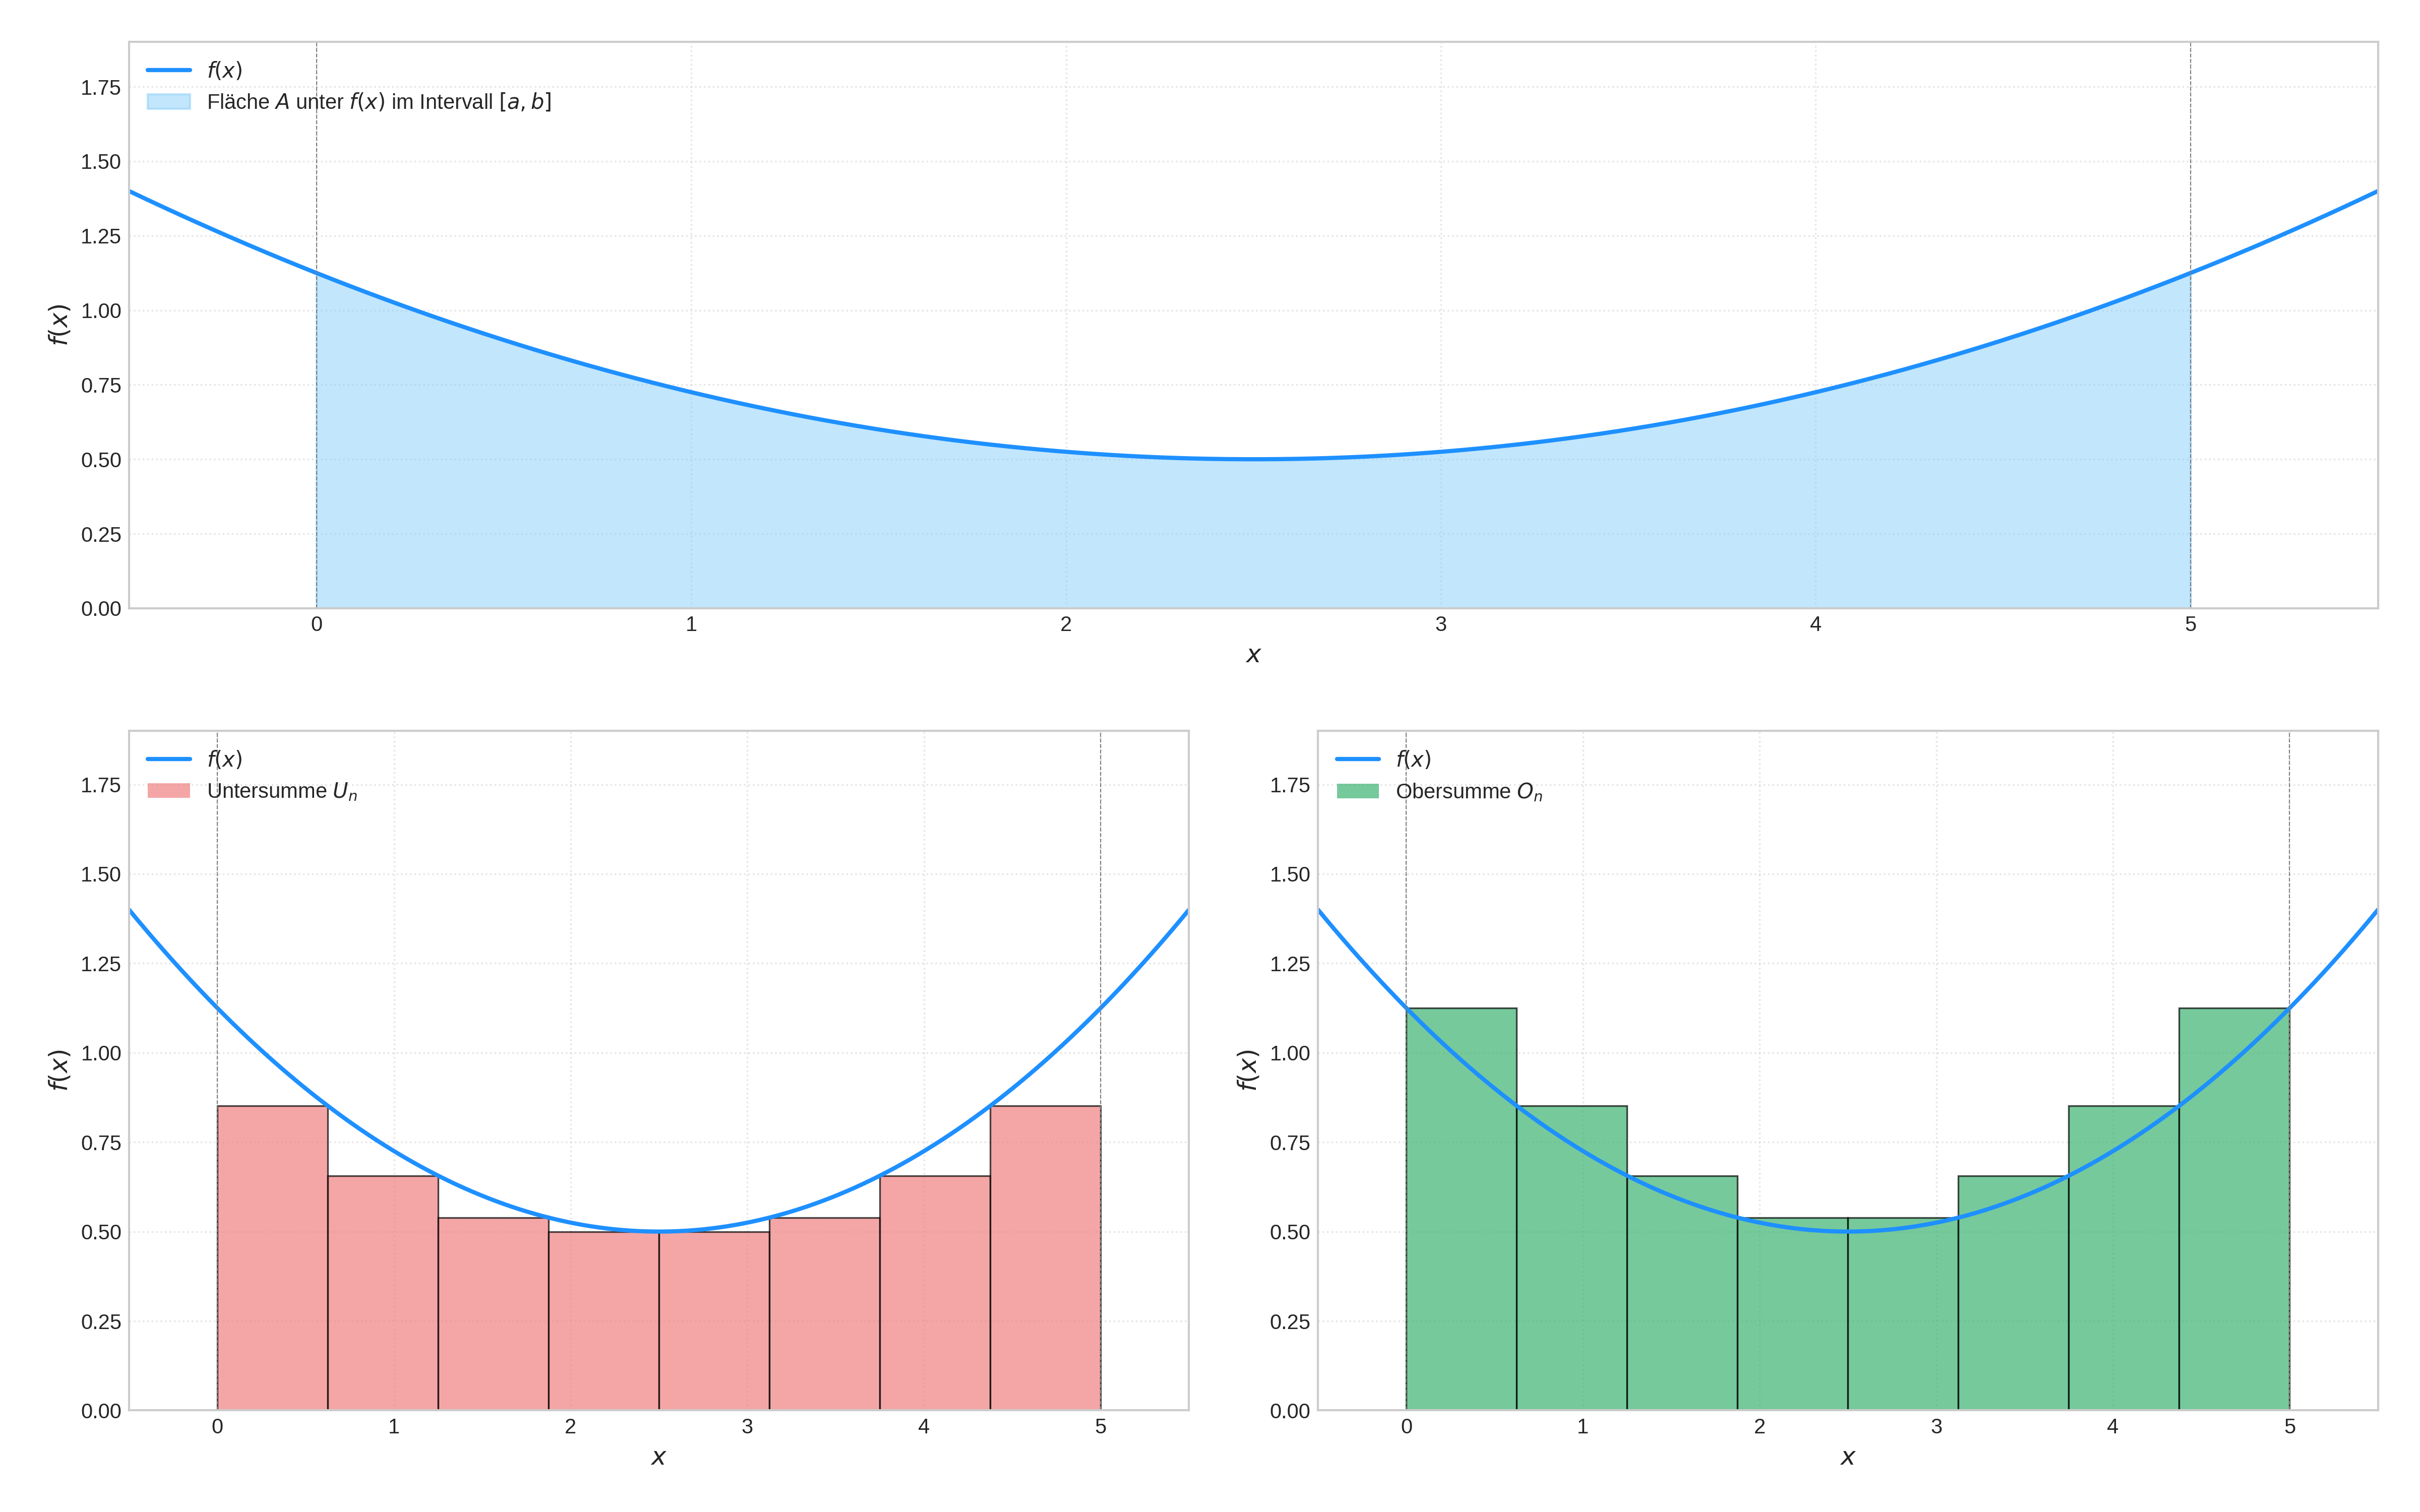
\includegraphics[width=0.9\textwidth]{grafiken/Riemannsummen_Untersumme_Obersumme.png}
    \captionof{figure}{Illustration von Untersumme und Obersumme (Riemannsummen)}
    \label{fig:riemannsummen_illustration}
\end{center}

Schauen wir uns ein konkretes Beispiel an, wie man eine Untersumme und eine Obersumme berechnet. Für einfache, monotone Funktionen ist die Bestimmung des Minimums/Maximums in einem Teilintervall einfach der Funktionswert am entsprechenden Rand.

\begin{beispielumgebung}{Untersumme und Obersumme für $f(x)=x^2$}
Wir wollen den Flächeninhalt unter der Funktion $f(x)=x^2$ im Intervall $[0,2]$ mit $n=4$ Teilintervallen durch Untersumme $U_4$ und Obersumme $O_4$ annähern.

\textbf{Schritt 1: Intervallbreite $\Delta x$ und Teilungspunkte $x_i$ bestimmen.}
Das Intervall ist $[a,b] = [0,2]$. Die Anzahl der Teilintervalle ist $n=4$.
Die Breite jedes Teilintervalls ist $\Delta x = \frac{b-a}{n} = \frac{2-0}{4} = \frac{2}{4} = 0.5$.
Die Teilungspunkte sind:
$x_0 = a = 0$
$x_1 = x_0 + \Delta x = 0 + 0.5 = 0.5$
$x_2 = x_1 + \Delta x = 0.5 + 0.5 = 1$
$x_3 = x_2 + \Delta x = 1 + 0.5 = 1.5$
$x_4 = x_3 + \Delta x = 1.5 + 0.5 = 2 (=b)$.

\textbf{Schritt 2: Untersumme $U_4$ berechnen.}
Die Funktion $f(x)=x^2$ ist im Intervall $[0,2]$ streng monoton steigend. Das bedeutet, der kleinste Funktionswert (Minimum) in jedem Teilintervall $[x_{i-1}, x_i]$ befindet sich am \textbf{linken Rand} $x_{i-1}$. Die Höhe des $i$-ten Rechtecks ist also $f(x_{i-1})$.
\begin{itemize}
    \item 1. Rechteck (Intervall $[x_0, x_1] = [0, 0.5]$): Höhe $f(x_0) = f(0) = 0^2 = 0$. Fläche $\Delta x \cdot f(0) = 0.5 \cdot 0 = 0$.
    \item 2. Rechteck (Intervall $[x_1, x_2] = [0.5, 1]$): Höhe $f(x_1) = f(0.5) = (0.5)^2 = 0.25$. Fläche $\Delta x \cdot f(0.5) = 0.5 \cdot 0.25 = 0.125$.
    \item 3. Rechteck (Intervall $[x_2, x_3] = [1, 1.5]$): Höhe $f(x_2) = f(1) = 1^2 = 1$. Fläche $\Delta x \cdot f(1) = 0.5 \cdot 1 = 0.5$.
    \item 4. Rechteck (Intervall $[x_3, x_4] = [1.5, 2]$): Höhe $f(x_3) = f(1.5) = (1.5)^2 = 2.25$. Fläche $\Delta x \cdot f(1.5) = 0.5 \cdot 2.25 = 1.125$.
\end{itemize}
Die Untersumme ist die Summe dieser Flächen:
$U_4 = 0 + 0.125 + 0.5 + 1.125 = 1.75$.

\textbf{Schritt 3: Obersumme $O_4$ berechnen.}
Da $f(x)=x^2$ im Intervall $[0,2]$ streng monoton steigend ist, liegt der größte Funktionswert (Maximum) in jedem Teilintervall $[x_{i-1}, x_i]$ am \textbf{rechten Rand} $x_i$. Die Höhe des $i$-ten Rechtecks ist also $f(x_i)$.
\begin{itemize}
    \item 1. Rechteck (Intervall $[x_0, x_1] = [0, 0.5]$): Höhe $f(x_1) = f(0.5) = (0.5)^2 = 0.25$. Fläche $\Delta x \cdot f(0.5) = 0.5 \cdot 0.25 = 0.125$.
    \item 2. Rechteck (Intervall $[x_1, x_2] = [0.5, 1]$): Höhe $f(x_2) = f(1) = 1^2 = 1$. Fläche $\Delta x \cdot f(1) = 0.5 \cdot 1 = 0.5$.
    \item 3. Rechteck (Intervall $[x_2, x_3] = [1, 1.5]$): Höhe $f(x_3) = f(1.5) = (1.5)^2 = 2.25$. Fläche $\Delta x \cdot f(1.5) = 0.5 \cdot 2.25 = 1.125$.
    \item 4. Rechteck (Intervall $[x_3, x_4] = [1.5, 2]$): Höhe $f(x_4) = f(2) = 2^2 = 4$. Fläche $\Delta x \cdot f(2) = 0.5 \cdot 4 = 2$.
\end{itemize}
Die Obersumme ist die Summe dieser Flächen:
$O_4 = 0.125 + 0.5 + 1.125 + 2 = 3.75$.

Der wahre Flächeninhalt $A$ unter $f(x)=x^2$ im Intervall $[0,2]$ liegt also zwischen $1.75$ und $3.75$:
$1.75 \le A \le 3.75$.
Wenn wir $n$ erhöhen, wird diese 'Schere' zwischen Unter- und Obersumme immer kleiner. Der exakte Wert ist übrigens $A = \frac{8}{3} \approx 2.667$. Unsere Näherungen sind also noch recht grob, aber sie zeigen das Prinzip.
\end{beispielumgebung}

\begin{tippumgebung}{Summenformel für Riemannsummen}
Allgemein lässt sich die Untersumme $U_n$ und Obersumme $O_n$ mit dem Summenzeichen $\sum$ schreiben:
Sei $m_i$ das Minimum von $f(x)$ im $i$-ten Teilintervall $[x_{i-1}, x_i]$ und $M_i$ das Maximum.
Dann ist:
\[ U_n = \sum_{i=1}^{n} m_i \cdot \Delta x \]
\[ O_n = \sum_{i=1}^{n} M_i \cdot \Delta x \]
Wenn $f(x)$ im Intervall $[a,b]$ monoton steigend ist, dann ist $m_i = f(x_{i-1})$ (linker Rand) und $M_i = f(x_i)$ (rechter Rand).
Wenn $f(x)$ im Intervall $[a,b]$ monoton fallend ist, dann ist $m_i = f(x_i)$ (rechter Rand) und $M_i = f(x_{i-1})$ (linker Rand).
\end{tippumgebung}

\begin{aufgabenumgebung}{Riemannsummen berechnen}
Gegeben ist die Funktion $f(x) = x+1$.
\begin{enumerate}
    \item Berechne die Untersumme $U_5$ und die Obersumme $O_5$ für das Intervall $[0,5]$ mit $n=5$ Teilintervallen.
    \begin{tippumgebung}{Monotonie}
    Ist $f(x)=x+1$ monoton steigend oder fallend? Wo liegt also das Minimum bzw. Maximum in jedem Teilintervall?
    \end{tippumgebung}
    \item Der Graph von $f(x)=x+1$ ist eine Gerade. Der Bereich unter dem Graphen im Intervall $[0,5]$ bildet ein Trapez. Berechne den exakten Flächeninhalt dieses Trapezes mit der geometrischen Formel $A_{Trapez} = \frac{(a+c)}{2} \cdot h$ (wobei $a$ und $c$ die parallelen Seiten sind und $h$ die Höhe).
    \item Vergleiche deine Ergebnisse für $U_5$ und $O_5$ mit dem exakten Flächeninhalt.
    \item Was würde passieren, wenn du $n=10$ oder $n=100$ Teilintervalle wählen würdest? Wie würden sich $U_n$ und $O_n$ verändern?
\end{enumerate}

\begin{center}
    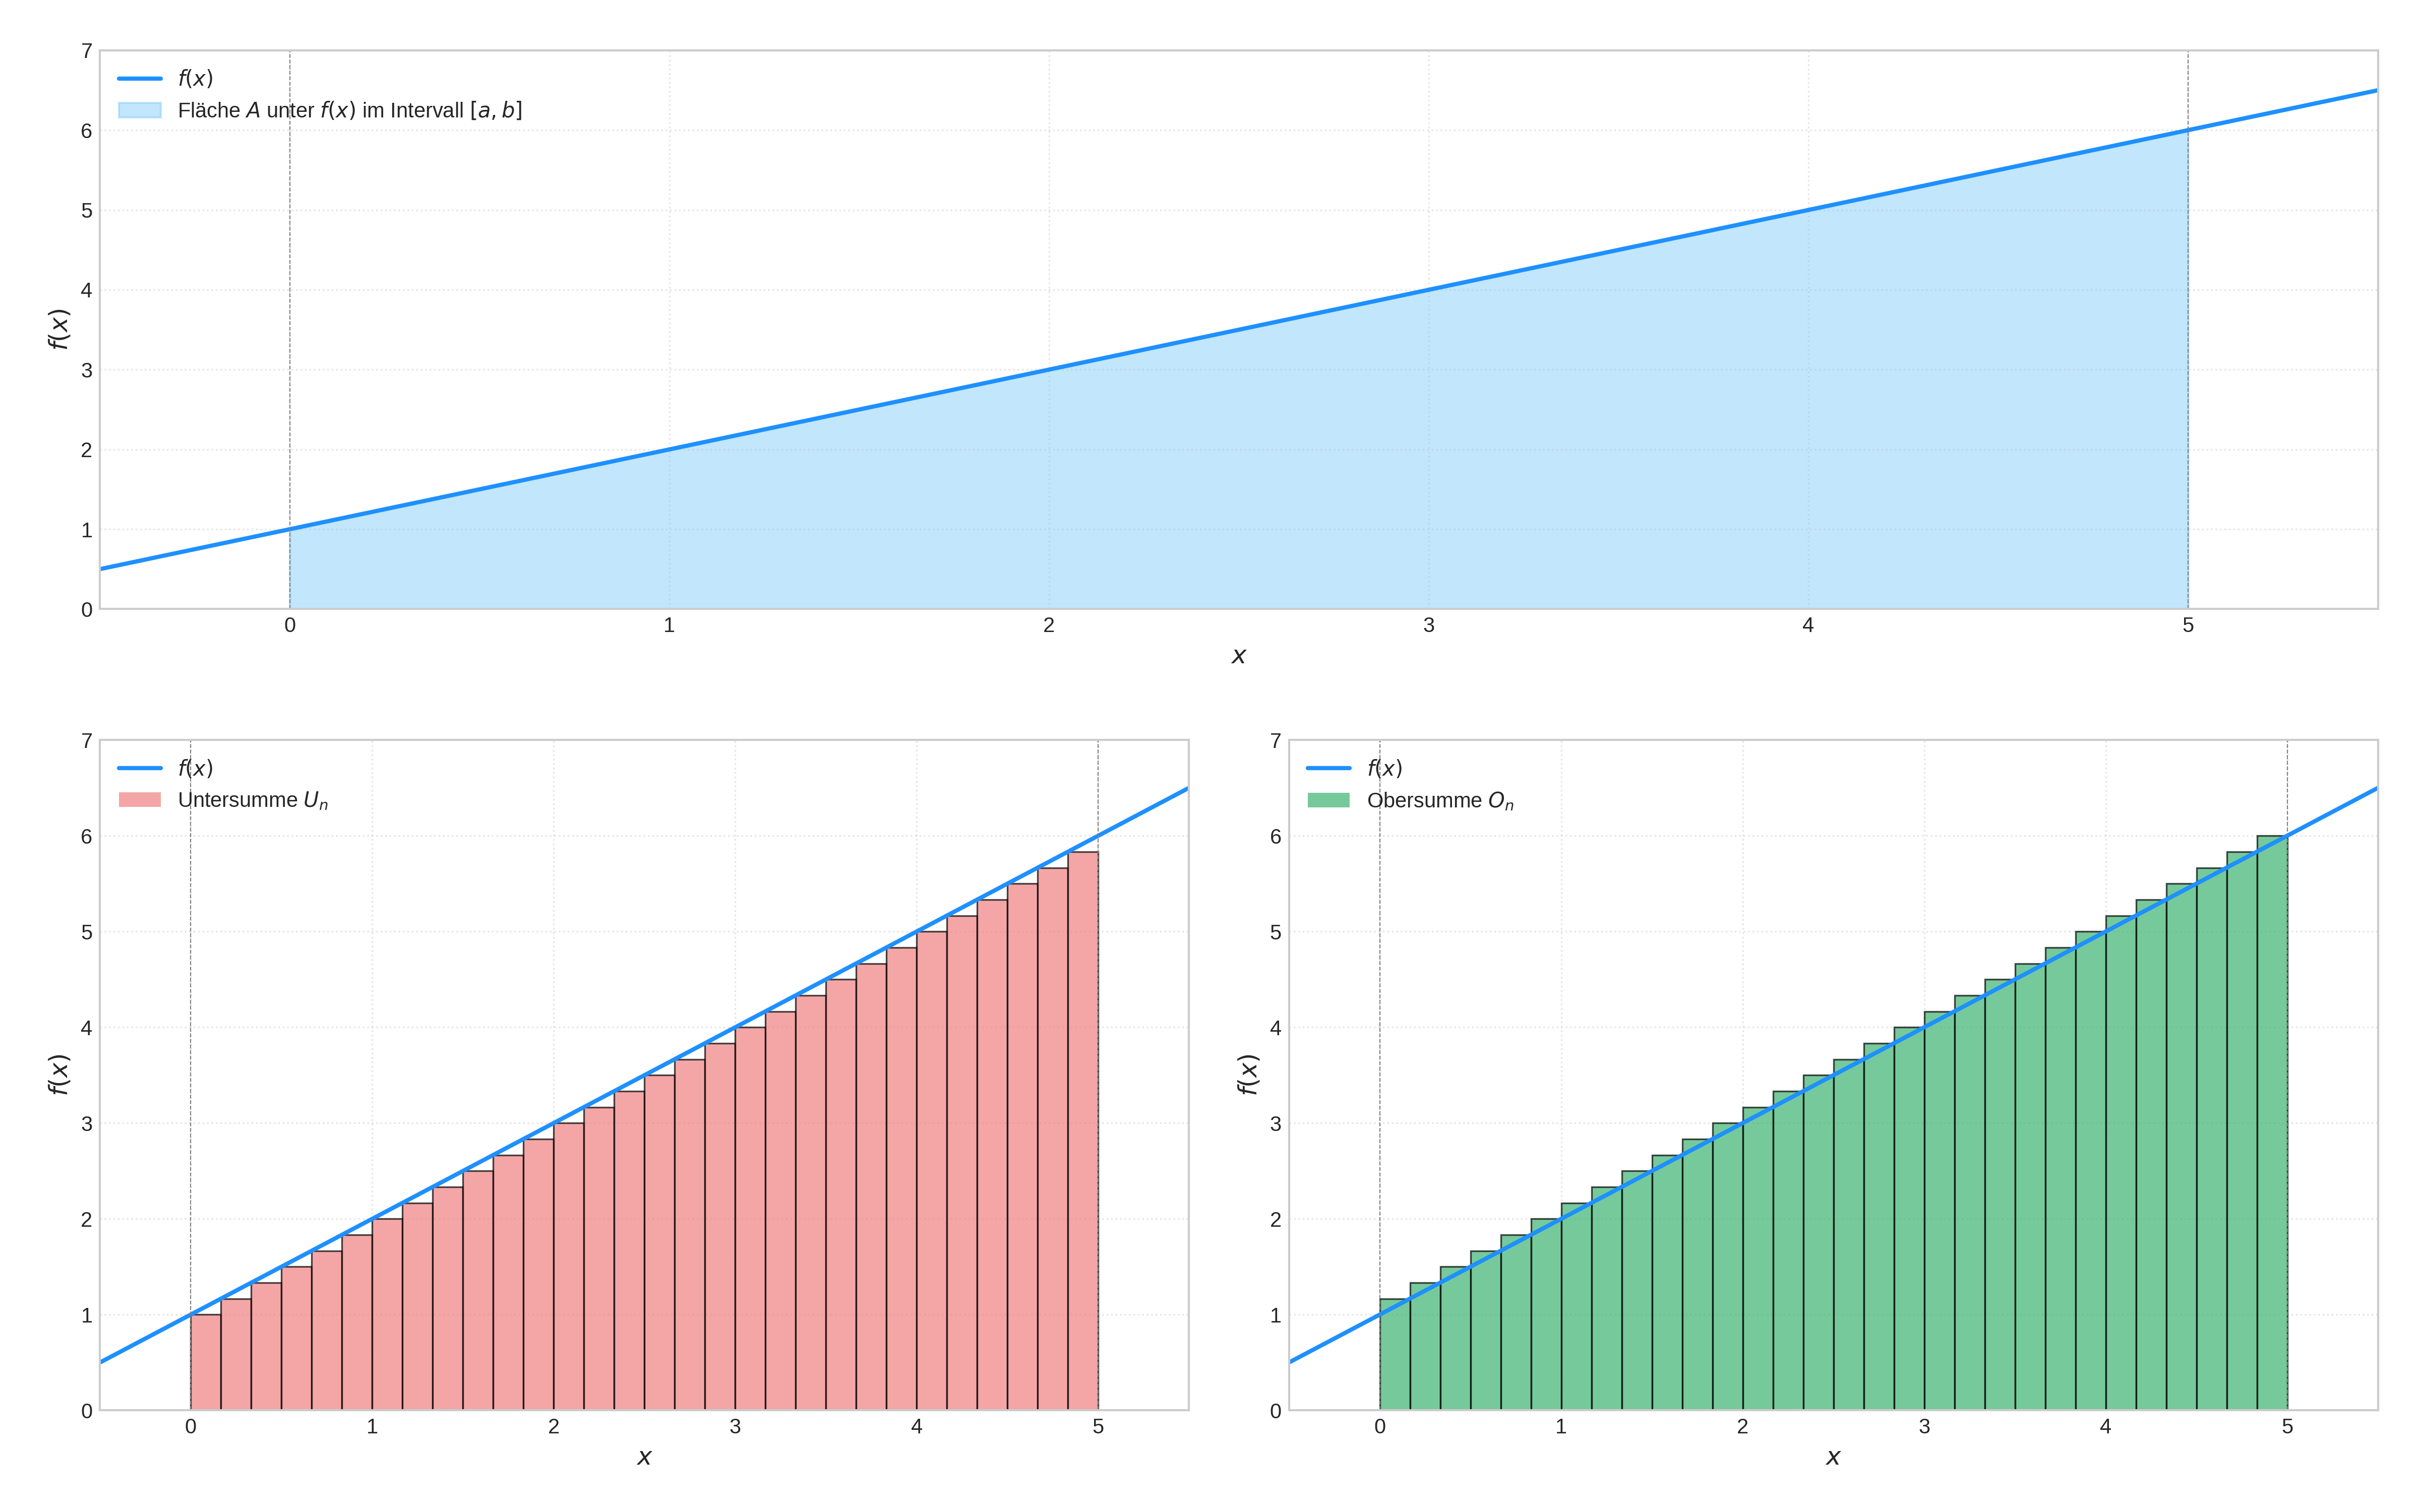
\includegraphics[width=0.9\textwidth]{grafiken/Riemannsummen_lineareFunktion.png}
    \captionof{figure}{Fläche unter $f(x)=x+1$ im Intervall $[0,5]$ }
    \label{fig:riemannsummen_linear_illustration}
\end{center}
\end{aufgabenumgebung}

Die Idee der Riemannsummen führt uns direkt zum Begriff des \textbf{bestimmten Integrals}.

\subsection{Das bestimmte Integral – Der exakte Flächeninhalt}
\label{subsec:bestimmtes_integral_neu} % Neues Label

Wir haben gesehen, dass wir den Flächeninhalt unter einer Kurve durch Riemannsummen (z.B. Unter- und Obersummen) annähern können. Je mehr Rechtecke wir verwenden (je größer $n$ wird und damit je kleiner $\Delta x = \frac{b-a}{n}$ wird), desto genauer wird unsere Näherung.

Wenn wir diesen Prozess ins Unendliche treiben, also $n \to \infty$ (und damit $\Delta x \to 0$), dann konvergieren die Untersumme und die Obersumme (für 'nette', d.h. integrierbare Funktionen) gegen denselben Wert. Dieser gemeinsame Grenzwert ist der exakte Flächeninhalt unter der Kurve und wird als das \textbf{bestimmte Integral} der Funktion $f(x)$ von $a$ bis $b$ bezeichnet.

\begin{merksatzumgebung}{Das bestimmte Integral}
Das \textbf{bestimmte Integral} einer Funktion $f(x)$ im Intervall $[a,b]$ ist der Grenzwert der Riemannsummen, wenn die Anzahl der Teilintervalle $n$ gegen unendlich geht (und die Breite $\Delta x$ der Teilintervalle gegen Null geht):
\[ \int_{a}^{b} f(x) \,dx = \lim_{n \to \infty} \sum_{i=1}^{n} f(x_i^*) \cdot \Delta x \]
Dabei ist:
\begin{itemize}
    \item $\int$ das \textbf{Integrationszeichen} (ein stilisiertes S für 'Summe').
    \item $a$ die \textbf{untere Integrationsgrenze}.
    \item $b$ die \textbf{obere Integrationsgrenze}.
    \item $f(x)$ der \textbf{Integrand} (die zu integrierende Funktion).
    \item $dx$ das \textbf{Differential}, das anzeigt, nach welcher Variablen integriert wird (hier $x$) und symbolisiert die unendlich kleine Breite der Rechtecke.
\end{itemize}
Wenn $f(x) \ge 0$ im Intervall $[a,b]$ ist, dann gibt $\int_{a}^{b} f(x) \,dx$ den \textbf{Flächeninhalt} der Fläche an, die vom Graphen von $f(x)$, der x-Achse und den senkrechten Geraden $x=a$ und $x=b$ eingeschlossen wird.
\end{merksatzumgebung}

\begin{infoboxumgebung}{Was passiert, wenn $f(x)$ unterhalb der x-Achse liegt?}
Wenn der Graph von $f(x)$ in einem Intervall unterhalb der x-Achse verläuft (also $f(x) < 0$), dann liefert das bestimmte Integral in diesem Bereich einen \textbf{negativen Wert}. Dieser negative Wert entspricht dem Flächeninhalt zwischen dem Graphen und der x-Achse, aber eben mit negativem Vorzeichen.
Man spricht dann von einer \textbf{orientierten Fläche}. Flächenanteile oberhalb der x-Achse zählen positiv, Flächenanteile unterhalb der x-Achse zählen negativ.
Um den 'echten' geometrischen Flächeninhalt zu bekommen, wenn Teile unterhalb liegen, muss man die Beträge der entsprechenden Integrale addieren oder die Funktion an den entsprechenden Stellen spiegeln (also $|f(x)|$ integrieren).
\begin{center}
    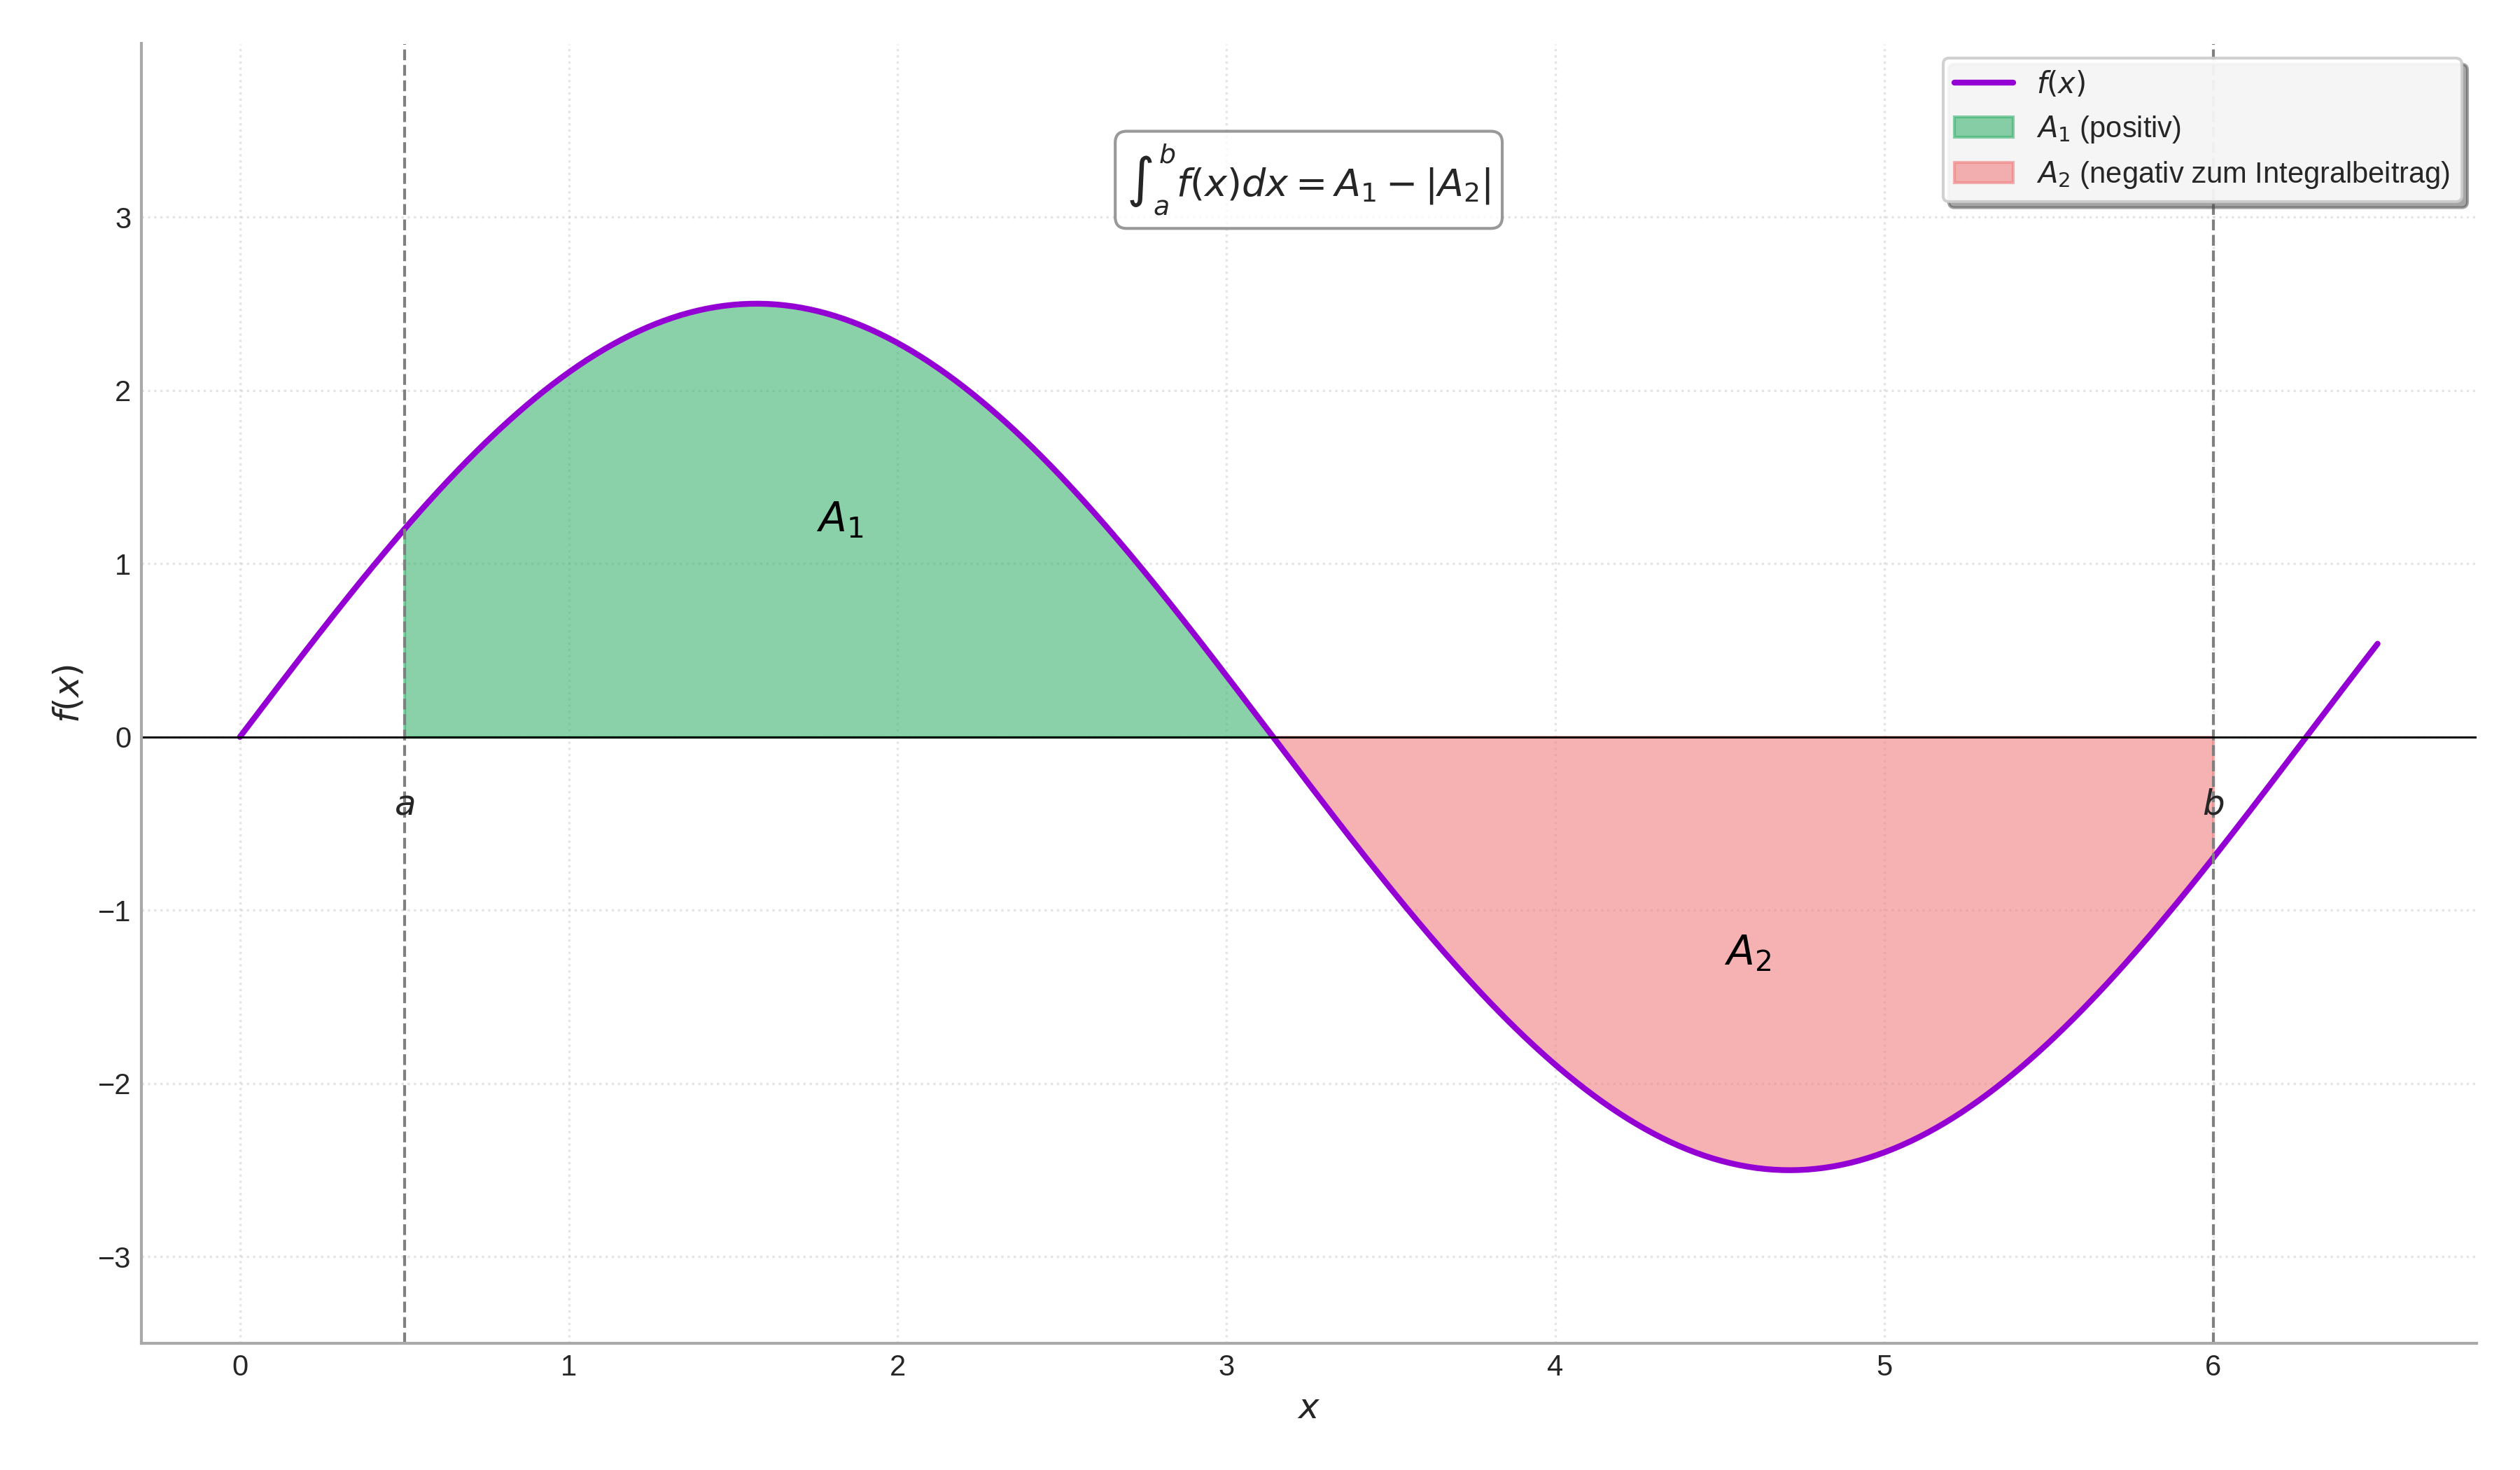
\includegraphics[width=0.8\textwidth]{grafiken/Integral_Orientierte_Flaeche.png}
    \captionof{figure}{Orientierter Flächeninhalt beim bestimmten Integral}
    \label{fig:orientierte_flaeche}
\end{center}
\end{infoboxumgebung}

\begin{fehlerboxumgebung}{Orientierte vs. geometrische Fläche – Genau hinschauen!}
Das bestimmte Integral liefert die Flächenbilanz, nicht immer den rein geometrischen Flächeninhalt!
\begin{itemize}
    \item \textbf{Orientierte Fläche:} Das Ergebnis von $\int_a^b f(x)dx$ ist die \textbf{Summe der vorzeichenbehafteten Flächenstücke}. Flächen über der x-Achse gehen positiv ein, Flächen darunter negativ.
    \item \textbf{Geometrischer Gesamtflächeninhalt gesucht?} Wenn die Aufgabe nach dem tatsächlichen, sichtbaren Flächeninhalt zwischen Graph und x-Achse fragt, musst du aufpassen:
    \begin{itemize}
        \item \textbf{Nullstellen prüfen:} Bestimme immer zuerst die Nullstellen von $f(x)$ im Intervall $[a,b]$. Diese teilen das Gesamtintervall eventuell in Teilintervalle auf.
        \item \textbf{Teilintervalle betrachten:} Untersuche das Vorzeichen von $f(x)$ in jedem Teilintervall.
        \item \textbf{Beträge addieren:} Für Teilintervalle, in denen $f(x) < 0$ (Graph unter der x-Achse), ist das Integral negativ. Für den geometrischen Flächeninhalt musst du den \textbf{Betrag} dieses negativen Wertes nehmen und zu den positiven Flächenanteilen addieren.
    \end{itemize}
    \item \textbf{Negatives Integral $\neq$ Rechenfehler:} Ein negatives Ergebnis für ein bestimmtes Integral ist oft korrekt und bedeutet lediglich, dass der Flächenanteil unterhalb der x-Achse im betrachteten Intervall überwiegt (oder die gesamte Fläche unterhalb liegt).
\end{itemize}
\end{fehlerboxumgebung}

Die Berechnung von Integralen über den Grenzwert von Riemannsummen ist sehr aufwendig. Glücklicherweise gibt es einen viel eleganteren Weg, der die Integralrechnung mit der Differentialrechnung verbindet: den Hauptsatz der Differential- und Integralrechnung. Dafür benötigen wir aber zuerst das Konzept der Stammfunktion.

\subsection{Die Stammfunktion – Das 'Gegenteil' vom Ableiten (Aufleiten)}
\label{subsec:stammfunktion_integral} % Neues Label

In der Differentialrechnung haben wir gelernt, zu einer gegebenen Funktion $f(x)$ ihre Ableitungsfunktion $f'(x)$ zu finden, die uns die Steigung von $f(x)$ an jeder Stelle liefert.
Die Integralrechnung stellt nun oft die umgekehrte Frage:
\textit{Wenn wir eine Funktion $f(x)$ gegeben haben (die wir uns jetzt als Ableitung einer anderen Funktion vorstellen können), welche Funktion $F(x)$ müssen wir ableiten, um genau dieses $f(x)$ als Ergebnis zu erhalten?}
Eine solche Funktion $F(x)$ nennen wir eine \textbf{Stammfunktion} von $f(x)$.

\begin{merksatzumgebung}{Stammfunktion}
Eine Funktion $F(x)$ heißt \textbf{Stammfunktion} einer Funktion $f(x)$, wenn für alle $x$ im Definitionsbereich gilt:
\[ F'(x) = f(x) \]
Das bedeutet, die Ableitung der Stammfunktion $F(x)$ ergibt die ursprüngliche Funktion $f(x)$.
Den Vorgang des Findens einer Stammfunktion nennt man auch \textbf{Integrieren} oder umgangssprachlich (und sehr anschaulich) \textbf{Aufleiten}.
\end{merksatzumgebung}

Das Finden von Stammfunktionen ist also wie ein Rätsel: 'Welche Funktion wurde hier abgeleitet?'

\begin{beispielumgebung}{Stammfunktionen finden durch 'Rückwärts-Ableiten'}
\begin{enumerate}
    \item \textbf{Gegeben: $f(x) = 2x$.}
        Wir fragen uns: Welche Funktion $F(x)$ hat als Ableitung $2x$?
        Aus der Potenzregel der Ableitung wissen wir: $(x^2)' = 2x^1 = 2x$.
        Also ist $F(x) = x^2$ eine Stammfunktion von $f(x)=2x$.

        \textit{Aber Moment mal!} Was ist mit $F_1(x) = x^2 + 5$?
        $F_1'(x) = (x^2)' + (5)' = 2x + 0 = 2x$.
        Auch $F_1(x) = x^2+5$ ist eine Stammfunktion von $f(x)=2x$.

        Und was ist mit $F_2(x) = x^2 - 17$?
        $F_2'(x) = (x^2)' - (17)' = 2x - 0 = 2x$.
        Ebenfalls eine Stammfunktion!

        Es scheint unendlich viele Stammfunktionen zu geben, die sich nur durch eine additive Konstante unterscheiden.

    \item \textbf{Gegeben: $f(x) = x^2$.}
        Welche Funktion $F(x)$ ergibt abgeleitet $x^2$?
        Wir wissen, beim Ableiten wird der Exponent um 1 kleiner. Also muss der Exponent der Stammfunktion um 1 größer sein, also $x^3$.
        Probieren wir $G(x)=x^3$. Die Ableitung ist $G'(x)=3x^2$.
        Das ist noch nicht ganz $x^2$, sondern das Dreifache. Um das auszugleichen, müssen wir $x^3$ durch 3 teilen:
        $F(x) = \frac{1}{3}x^3$.
        Machen wir die Probe: $F'(x) = (\frac{1}{3}x^3)' = \frac{1}{3} \cdot (3x^2) = x^2$. Perfekt!
        Also ist $F(x) = \frac{1}{3}x^3$ eine Stammfunktion von $f(x)=x^2$.
        Und natürlich sind auch $F(x) = \frac{1}{3}x^3 + 7$ oder $F(x) = \frac{1}{3}x^3 - \pi$ Stammfunktionen.
\end{enumerate}
\end{beispielumgebung}

Das erste Beispiel hat uns eine wichtige Eigenschaft gezeigt:

\begin{merksatzumgebung}{Die Menge aller Stammfunktionen (Das unbestimmte Integral)}
Wenn $F(x)$ eine Stammfunktion einer Funktion $f(x)$ ist (d.h. $F'(x)=f(x)$), dann ist auch jede Funktion der Form $F(x)+C$, wobei $C$ eine beliebige reelle Konstante ist, eine Stammfunktion von $f(x)$.
Denn $(F(x)+C)' = F'(x) + (C)' = f(x) + 0 = f(x)$.

Die Menge aller dieser Stammfunktionen wird als das \textbf{unbestimmte Integral} von $f(x)$ bezeichnet und man schreibt dafür:
\[ \int f(x) \,dx = F(x) + C \]
Dabei ist:
\begin{itemize}
    \item $\int$ das \textbf{Integrationszeichen} (ein stilisiertes S, das an 'Summe' erinnert – ein Hinweis auf die Riemannsummen, die wir später kennenlernen).
    \item $f(x)$ der \textbf{Integrand} (die Funktion, die integriert/aufgeleitet wird).
    \item $dx$ das \textbf{Differential}, das anzeigt, nach welcher Variablen integriert wird (hier $x$). Es ist ein wichtiger Bestandteil der Notation.
    \item $F(x)$ irgendeine spezielle Stammfunktion von $f(x)$.
    \item $C$ die \textbf{Integrationskonstante} (eine beliebige reelle Zahl).
\end{itemize}
Das unbestimmte Integral liefert uns also nicht nur eine einzelne Funktion, sondern eine ganze \textbf{Schar von Funktionen}, die sich alle nur durch eine Verschiebung entlang der y-Achse unterscheiden.
\end{merksatzumgebung}

\textit{Selbst-Check:} Warum ist es wichtig, die Integrationskonstante $C$ beim unbestimmten Integral anzugeben? (Antwort: Weil es unendlich viele Funktionen gibt, deren Ableitung $f(x)$ ist, und $C$ repräsentiert all diese Möglichkeiten.)

\subsubsection{Grundlegende Integrationsregeln (Umkehrung der Ableitungsregeln)}
Ähnlich wie beim Ableiten gibt es auch beim Integrieren Regeln, die uns helfen, Stammfunktionen systematisch zu finden. Viele davon ergeben sich direkt durch Umkehrung der uns bekannten Ableitungsregeln. Wir konzentrieren uns hier zunächst auf Regeln für Polynomfunktionen.

\begin{merksatzumgebung}{Grundlegende Integrationsregeln für Polynome}
\begin{itemize}
    \item \textbf{Potenzregel der Integration:} Für $f(x) = x^n$ (mit $n \in \mathbb{R}, n \neq -1$) gilt:
    \[ \int x^n \,dx = \frac{1}{n+1}x^{n+1} + C \]
    \textit{Regel in Worten:} 'Erhöhe den Exponenten um 1 und teile dann durch diesen neuen Exponenten.'
    \textit{Beachte:} Diese Regel gilt nicht für $n=-1$, also für $f(x)=x^{-1}=\frac{1}{x}$. Die Stammfunktion von $\frac{1}{x}$ ist $\ln|x|+C$. Dies werden wir später bei den Logarithmusfunktionen genauer betrachten. Für Polynome tritt dieser Fall aber nicht auf.

    \item \textbf{Faktorregel der Integration:} Ein konstanter Faktor $k$ kann vor das Integral gezogen werden:
    \[ \int k \cdot f(x) \,dx = k \cdot \int f(x) \,dx \]
    Das bedeutet, wir können erst die Stammfunktion von $f(x)$ finden und diese dann mit $k$ multiplizieren.

    \item \textbf{Summenregel der Integration:} Das Integral einer Summe (oder Differenz) von Funktionen ist die Summe (oder Differenz) ihrer Integrale:
    \[ \int (f(x) \pm g(x)) \,dx = \int f(x) \,dx \pm \int g(x) \,dx \]
    \textit{Regel in Worten:} 'Jeder Summand wird für sich integriert/aufgeleitet, und die Ergebnisse werden dann addiert bzw. subtrahiert.'

    \item \textbf{Integral einer Konstanten:} Für $f(x)=k$ (eine Konstante) gilt:
    \[ \int k \,dx = kx + C \]
    (Denn die Ableitung von $kx+C$ ist $k$.)
\end{itemize}
\end{merksatzumgebung}

\begin{beispielumgebung}{Stammfunktionen mit Regeln bilden}
\begin{enumerate}
    \item \textbf{Bestimme $\int x^4 \,dx$.}
        Hier ist $n=4$. Nach der Potenzregel der Integration:
        $\int x^4 \,dx = \frac{1}{4+1}x^{4+1} + C = \frac{1}{5}x^5 + C$.
        \textit{Probe durch Ableiten:} $(\frac{1}{5}x^5+C)' = \frac{1}{5} \cdot 5x^4 + 0 = x^4$. Stimmt.

    \item \textbf{Bestimme $\int 6x^2 \,dx$.}
        Nach Faktor- und Potenzregel:
        $\int 6x^2 \,dx = 6 \cdot \int x^2 \,dx = 6 \cdot \left(\frac{1}{2+1}x^{2+1}\right) + C = 6 \cdot \frac{1}{3}x^3 + C = 2x^3 + C$.
        \textit{Probe:} $(2x^3+C)' = 2 \cdot 3x^2 + 0 = 6x^2$. Stimmt.

    \item \textbf{Bestimme $\int (3x^2 - 4x + 5) \,dx$.}
        Nach Summen-, Faktor- und Potenzregel:
        $\int (3x^2 - 4x + 5) \,dx = \int 3x^2 \,dx - \int 4x \,dx + \int 5 \,dx$
        $= 3 \cdot \int x^2 \,dx - 4 \cdot \int x^1 \,dx + \int 5x^0 \,dx$
        $= 3 \cdot \left(\frac{1}{3}x^3\right) - 4 \cdot \left(\frac{1}{2}x^2\right) + 5 \cdot \left(\frac{1}{1}x^1\right) + C$
        $= x^3 - 2x^2 + 5x + C$.
        \textit{Probe:} $(x^3 - 2x^2 + 5x + C)' = 3x^2 - 4x + 5$. Stimmt.
\end{enumerate}
\end{beispielumgebung}

\begin{aufgabenumgebung}{Stammfunktionen bilden üben}
Bestimme jeweils die Menge aller Stammfunktionen (das unbestimmte Integral) für die folgenden Funktionen:
\begin{enumerate}
    \item $f(x) = x^5$
    \item $g(x) = 12x^3$
    \item $h(x) = 2x^3 - 7x^2 + 4x - 1$
    \item $k(x) = \sqrt{x} + \frac{1}{x^3}$ (Tipp: Erst in Potenzschreibweise $x^n$ umwandeln! $\sqrt{x}=x^{1/2}$ und $\frac{1}{x^3}=x^{-3}$)
    \item $m(t) = at+b$ (wobei $a,b$ Konstanten sind; integriere nach $t$)
    \item $p(x) = (x+1)(x-2)$ (Tipp: Erst ausmultiplizieren!)
\end{enumerate}
Mache bei mindestens zwei Aufgaben die Probe durch Ableiten deiner Stammfunktion.
\end{aufgabenumgebung}

\begin{fehlerboxumgebung}{Integrationskonstante $C$ nicht vergessen!}
Ein sehr häufiger Fehler beim unbestimmten Integrieren ist das Vergessen der Integrationskonstante $+C$. Da die Ableitung einer Konstanten immer Null ist, gibt es zu jeder Funktion unendlich viele Stammfunktionen, die sich alle nur durch diese Konstante unterscheiden. Bei bestimmten Integralen (mit Grenzen) fällt diese Konstante später heraus, aber beim unbestimmten Integral ist sie wichtig! Stell dir vor, jede Stammfunktion ist wie ein Mitglied einer großen Familie von Kurven, die alle parallel zueinander verlaufen.
\end{fehlerboxumgebung}

\begin{warumwichtigumgebung}{Stammfunktionen und das unbestimmte Integral}
Das Konzept der Stammfunktion ist der Schlüssel, um den fundamentalen Zusammenhang zwischen Differential- und Integralrechnung zu verstehen. Es erlaubt uns, von einer gegebenen Änderungsrate auf die ursprüngliche Größe zurückzuschließen. Das unbestimmte Integral gibt uns die Gesamtheit aller möglichen Funktionen an, deren Ableitung die gegebene Funktion ist. Diese 'Familie' von Stammfunktionen wird entscheidend sein, wenn wir uns gleich dem bestimmten Integral und dem Hauptsatz zuwenden.
\end{warumwichtigumgebung}

Als Nächstes werden wir sehen, wie die Stammfunktion uns auf elegante Weise hilft, bestimmte Integrale und damit Flächeninhalte zu berechnen, ohne den mühsamen Weg über Riemannsummen gehen zu müssen. Das ist die Kernaussage des Hauptsatzes der Differential- und Integralrechnung.

% Vorheriger Inhalt des Kapitels bis zur warumwichtigumgebung 'Stammfunktionen und das unbestimmte Integral'
% ... (siehe vorherige Canvas-Version) ...

% Hier geht es dann weiter mit dem Hauptsatz der Differential- und Integralrechnung.
% Dieser Kommentar wird durch den folgenden Inhalt ersetzt:

\subsection{Der Hauptsatz der Differential- und Integralrechnung (HDI)}
\label{subsec:hdi}

Wir haben gesehen, dass das Berechnen von Flächeninhalten über den Grenzwert von Riemannsummen ziemlich mühsam sein kann. Gibt es einen einfacheren Weg, um das bestimmte Integral $\int_a^b f(x) \,dx$ exakt zu berechnen, ohne unendlich viele Rechtecke addieren zu müssen? Die Antwort ist ein klares Ja, und sie liegt in einem der wichtigsten Sätze der gesamten Mathematik: dem \textbf{Hauptsatz der Differential- und Integralrechnung} (oft abgekürzt als HDI).

Dieser Satz stellt eine fundamentale Verbindung zwischen der Differentialrechnung (dem Ableiten) und der Integralrechnung (dem Aufleiten bzw. Flächenberechnen) her. Er ist so etwas wie die 'magische Brücke' zwischen diesen beiden großen Gebieten der Analysis.

\begin{merksatzumgebung}{Der Hauptsatz der Differential- und Integralrechnung (HDI)}
Sei $f(x)$ eine im Intervall $[a,b]$ stetige Funktion und $F(x)$ eine beliebige Stammfunktion von $f(x)$ (d.h. $F'(x) = f(x)$). Dann gilt für das bestimmte Integral von $f(x)$ über dem Intervall $[a,b]$:
\[ \int_{a}^{b} f(x) \,dx = [F(x)]_{a}^{b} = F(b) - F(a) \]
\textbf{In Worten:} Um das bestimmte Integral von $f(x)$ in den Grenzen von $a$ bis $b$ zu berechnen, bilde eine Stammfunktion $F(x)$ von $f(x)$, setze die obere Grenze $b$ in $F(x)$ ein, setze die untere Grenze $a$ in $F(x)$ ein und subtrahiere den zweiten Wert vom ersten.

Die Schreibweise $[F(x)]_{a}^{b}$ ist eine Kurzform für $F(b) - F(a)$.
\end{merksatzumgebung}

\begin{warumwichtigumgebung}{Die Bedeutung des HDI}
Der Hauptsatz ist revolutionär, weil er uns sagt: Statt komplizierte Grenzwerte von Summen zu berechnen, um eine Fläche zu finden, können wir einfach eine Stammfunktion suchen (was oft viel einfacher ist) und deren Werte an den Rändern des Intervalls auswerten! Das Ableiten und Integrieren sind also tatsächlich Umkehroperationen zueinander.
\end{warumwichtigumgebung}

Schauen wir uns an, wie man den HDI anwendet.

\begin{beispielumgebung}{Bestimmtes Integral mit dem HDI berechnen}
\begin{enumerate}
    \item \textbf{Fläche unter $f(x)=x^2$ im Intervall $[0,2]$} (Vergleiche mit dem Riemannsummen-Beispiel!)
        Wir wollen $\int_{0}^{2} x^2 \,dx$ berechnen.
        \begin{itemize}
            \item \textbf{Schritt 1: Stammfunktion $F(x)$ von $f(x)=x^2$ finden.}
            Mit der Potenzregel der Integration: $F(x) = \frac{1}{2+1}x^{2+1} = \frac{1}{3}x^3$. (Die Integrationskonstante $C$ können wir hier weglassen, da sie sich bei der Differenz $F(b)-F(a)$ ohnehin aufheben würde: $(F(b)+C) - (F(a)+C) = F(b)-F(a)$.)
            \item \textbf{Schritt 2: Grenzen einsetzen $F(b)-F(a)$.}
            Hier ist $a=0$ und $b=2$.
            $\int_{0}^{2} x^2 \,dx = [ \frac{1}{3}x^3 ]_{0}^{2} = F(2) - F(0)$
            $= \left(\frac{1}{3}(2)^3\right) - \left(\frac{1}{3}(0)^3\right)$
            $= \frac{1}{3} \cdot 8 - \frac{1}{3} \cdot 0 = \frac{8}{3} - 0 = \frac{8}{3}$.
        \end{itemize}
        Der exakte Flächeninhalt ist $\frac{8}{3} \approx 2.667$. Das passt viel besser zu unseren Riemannsummen-Näherungen ($U_4=1.75, O_4=3.75$) und war viel einfacher zu berechnen!

    \item \textbf{Berechne $\int_{1}^{3} (3x^2 - 4x + 5) \,dx$.}
        Der Integrand ist $f(x) = 3x^2 - 4x + 5$.
        \begin{itemize}
            \item \textbf{Schritt 1: Stammfunktion $F(x)$ finden.}
            $F(x) = x^3 - 2x^2 + 5x$. (Wir lassen $C$ weg.)
            \item \textbf{Schritt 2: Grenzen einsetzen.}
            $\int_{1}^{3} (3x^2 - 4x + 5) \,dx = [x^3 - 2x^2 + 5x]_{1}^{3}$
            $= F(3) - F(1)$
            $= ((3)^3 - 2(3)^2 + 5(3)) - ((1)^3 - 2(1)^2 + 5(1))$
            $= (27 - 2 \cdot 9 + 15) - (1 - 2 \cdot 1 + 5)$
            $= (27 - 18 + 15) - (1 - 2 + 5)$
            $= (9 + 15) - (4) = 24 - 4 = 20$.
        \end{itemize}
        Der Wert des bestimmten Integrals ist 20.
\end{enumerate}
\end{beispielumgebung}

\begin{fehlerboxumgebung}{Hauptsatz-Anwendung – Typische Stolpersteine}
Der Hauptsatz der Differential- und Integralrechnung (HDI) ist mächtig, aber bei der Anwendung lauern ein paar typische Fehlerquellen:
\begin{itemize}
    \item \textbf{Grenzen vertauscht ($F(a)-F(b)$ statt $F(b)-F(a)$):} Achte penibel auf die Reihenfolge: Immer 'Stammfunktion an der oberen Grenze' minus 'Stammfunktion an der unteren Grenze', also $F(b)-F(a)$. Ein Vertauschen führt zum Vorzeichenfehler im Ergebnis!
    \item \textbf{Rechenfehler beim Einsetzen der Grenzen:} Das ist eine der häufigsten Fehlerquellen!
    \begin{itemize}
        \item Besonders bei negativen Zahlen als Grenzen oder in der Stammfunktion: Setze sorgfältig Klammern, z.B. $F(-2) = \frac{1}{3}(-2)^3 - (-2) = -\frac{8}{3} + 2$.
        \item Brüche und Potenzen korrekt berechnen. Nimm dir Zeit für diesen Schritt.
    \end{itemize}
    \item \textbf{Stammfunktion $F(x)$ falsch gebildet:} Der HDI funktioniert nur, wenn $F(x)$ auch wirklich eine korrekte Stammfunktion von $f(x)$ ist. Überprüfe deine Integrationsregeln (Potenzregel, Faktorregel, Summenregel etc.) sorgfältig. Im Zweifel: Leite deine gefundene Stammfunktion $F(x)$ zur Probe ab – es muss wieder $f(x)$ herauskommen!
    \item \textbf{Integrationskonstante $C$ beim bestimmten Integral:} Für die Berechnung des bestimmten Integrals $\int_a^b f(x)dx = F(b)-F(a)$ kannst du die Integrationskonstante $C$ weglassen (oder $C=0$ setzen), da sie sich ohnehin herauskürzen würde: $(F(b)+C) - (F(a)+C) = F(b)-F(a)$. Wenn du sie mitschleppst, achte darauf, dass sie sich korrekt aufhebt.
\end{itemize}
Sorgfältiges und schrittweises Rechnen hilft, diese Fehler zu vermeiden!
\end{fehlerboxumgebung}

\begin{aufgabenumgebung}{Bestimmte Integrale mit dem HDI berechnen}
Berechne die folgenden bestimmten Integrale mit dem Hauptsatz.
\begin{enumerate}
    \item $\int_{1}^{2} (4x^3 - 6x) \,dx$
    \item $\int_{-1}^{1} (x^2 + 2) \,dx$
    \item $\int_{0}^{4} (\sqrt{x} + 1) \,dx$ (Tipp: $\sqrt{x} = x^{1/2}$)
    \item \textbf{Fläche visualisieren:}
        Die Funktion $f(x) = -x^2 + 4x$ hast du vielleicht schon in früheren Aufgaben skizziert (eine nach unten geöffnete Parabel).
        \begin{itemize}
            \item Berechne die Nullstellen von $f(x)$.
            \item Berechne das bestimmte Integral $\int_{x_1}^{x_2} f(x) \,dx$, wobei $x_1$ und $x_2$ die Nullstellen sind ($x_1 < x_2$).
            \item Was stellt dieser Wert geometrisch dar? Markiere die entsprechende Fläche in einer Skizze des Graphen von $f(x)$.
\begin{center}
    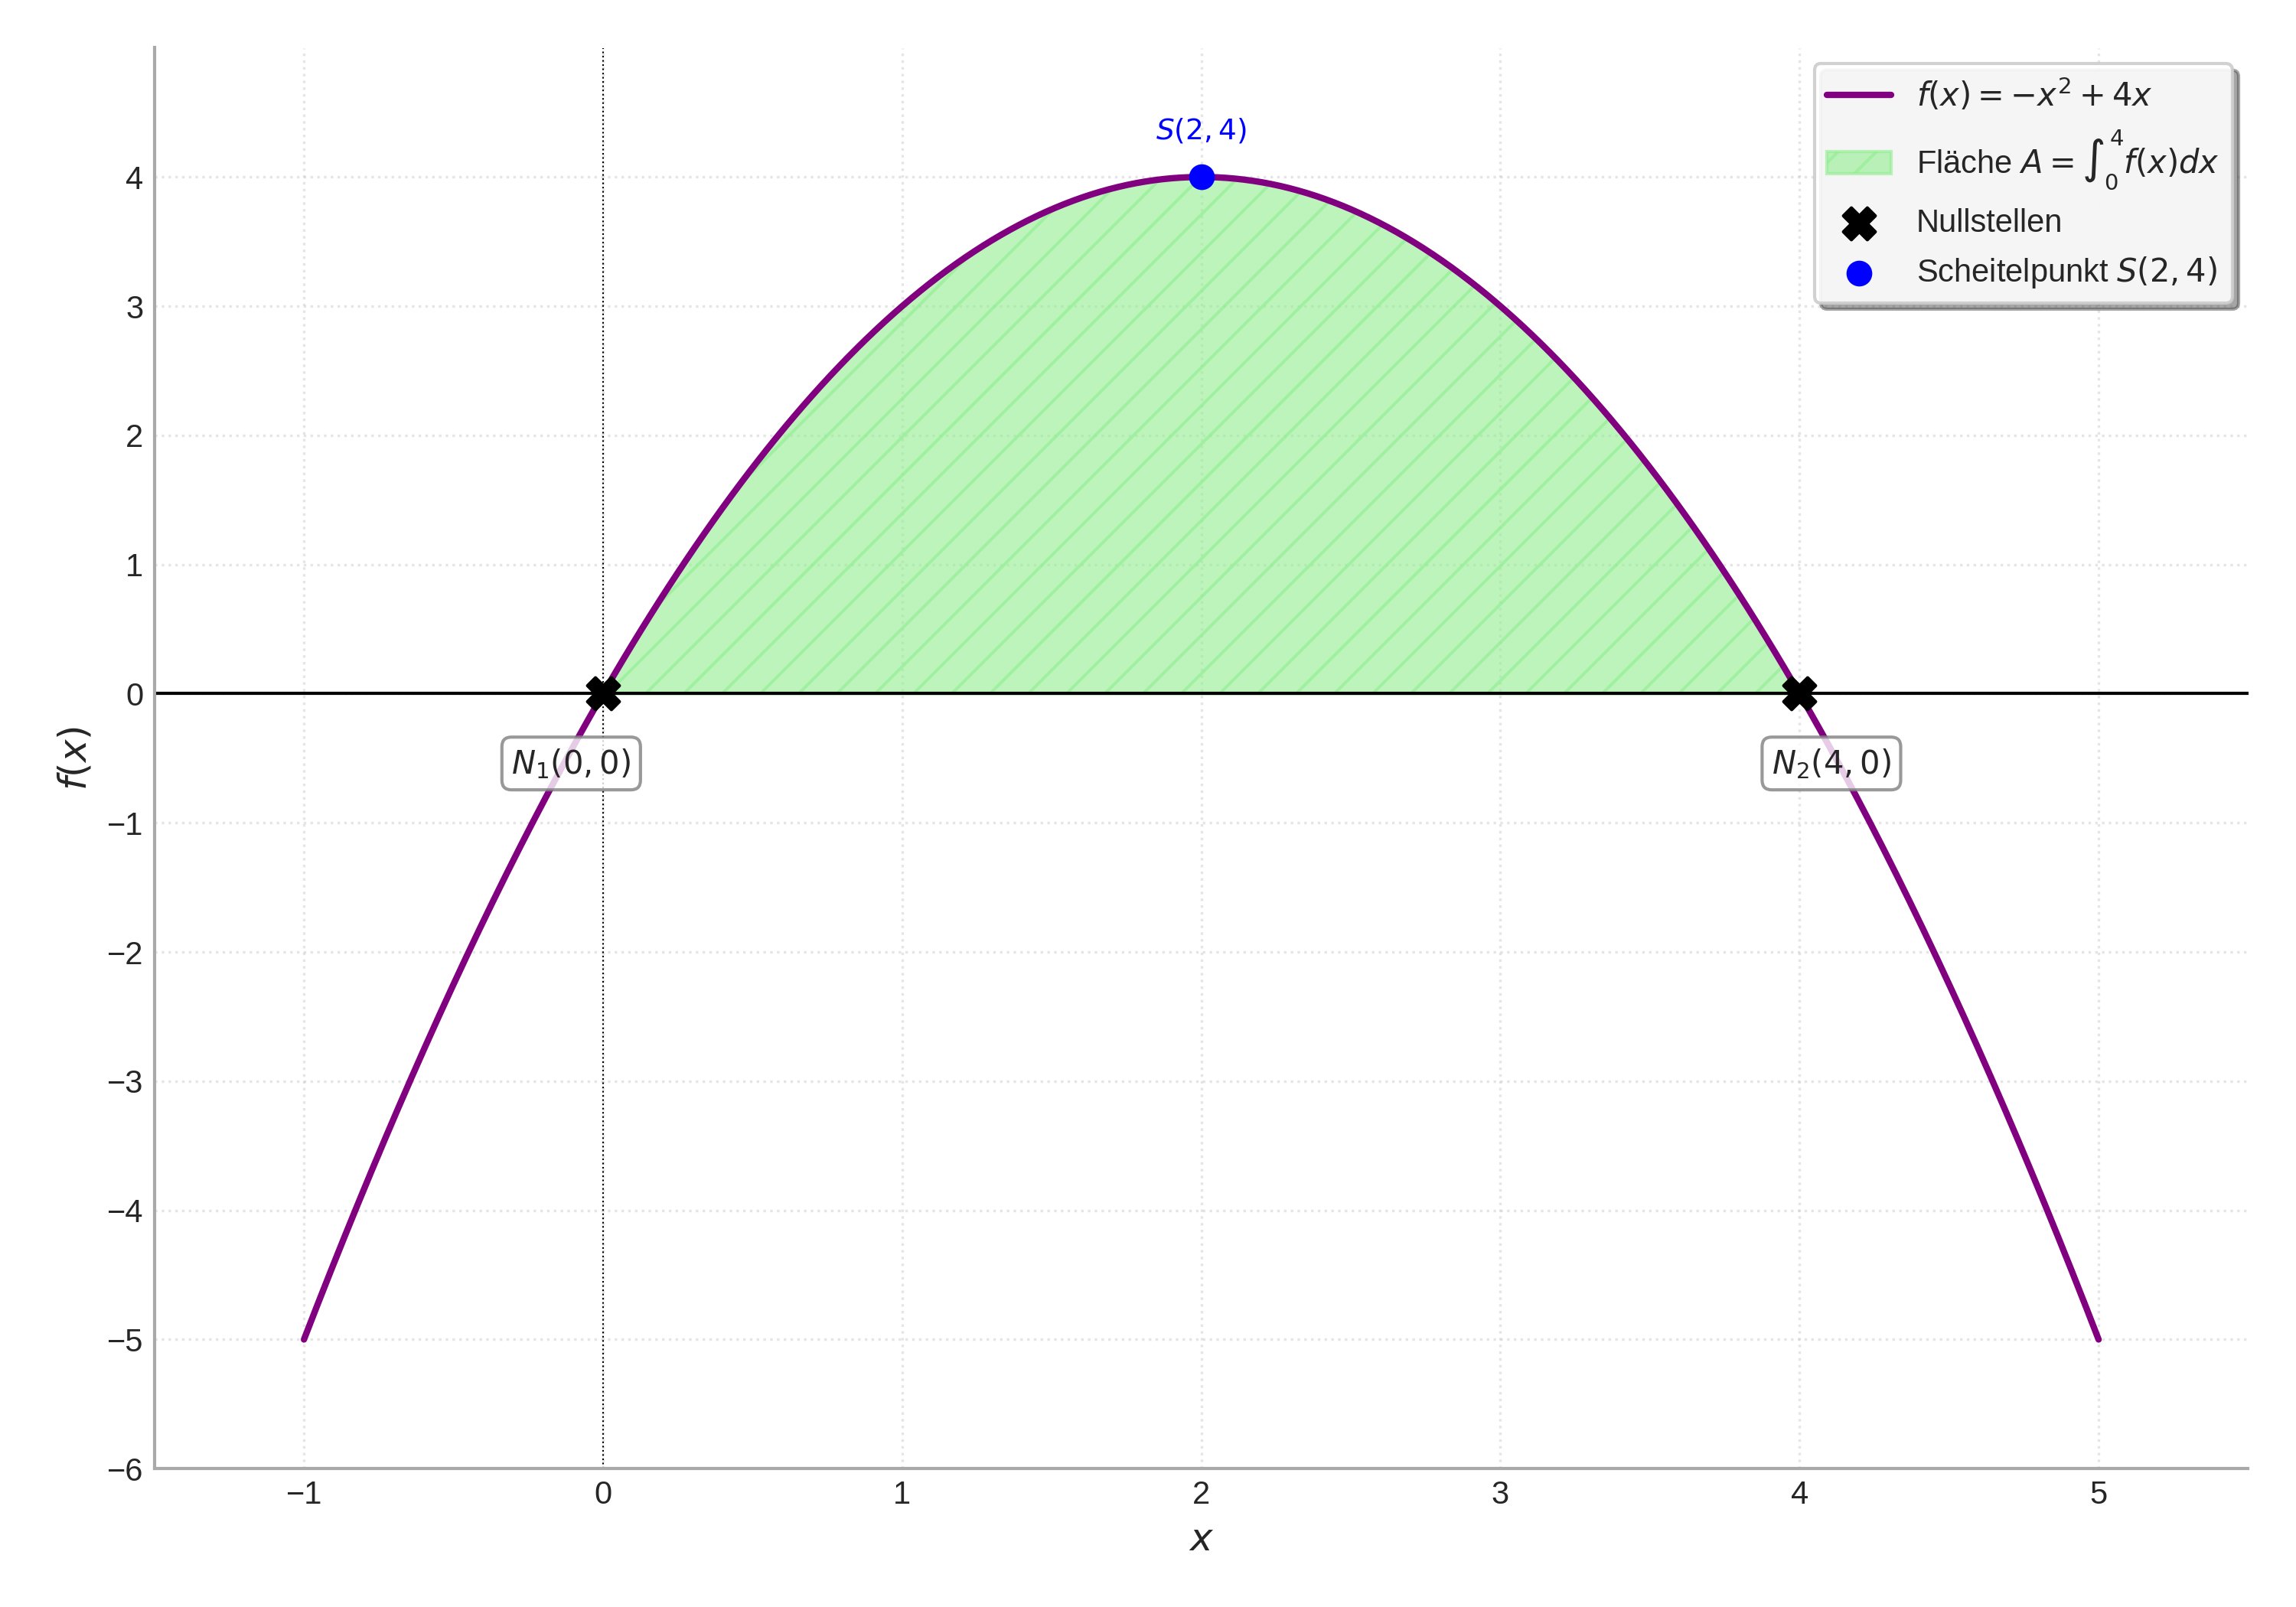
\includegraphics[width=0.8\textwidth]{grafiken/Integral_Flaeche_Parabel.png}
    \captionof{figure}{Fläche unter $f(x)=-x^2+4x$ zwischen den Nullstellen}
    \label{fig:flaeche_parabel}
\end{center}
        \end{itemize}
\end{enumerate}
\end{aufgabenumgebung}


\begin{funfactbox}{Newton, unendliche Reihen und die Quadratur des Kreises (fast!)}
Die Zahl $\pi$ fasziniert Mathematiker seit Jahrtausenden. Die alten Methoden zur Annäherung von $\pi$ waren oft geometrisch und extrem aufwendig. Isaac Newton fand um 1666 einen revolutionär neuen Weg, der die gerade erst entwickelte Analysis nutzte.

Seine Idee war, die Fläche eines Viertel-Einheitskreises zu berechnen, denn diese Fläche ist genau $\frac{\pi}{4}$. Die Gleichung eines Kreises mit Radius 1 ist $x^2+y^2=1$, also ist die obere Hälfte $y = \sqrt{1-x^2}$. Die Fläche des Viertelkreises im ersten Quadranten ist dann das bestimmte Integral:
\[ \text{Fläche} = \int_0^1 \sqrt{1-x^2} \,dx = \frac{\pi}{4} \]
Das Problem: Wie integriert man $\sqrt{1-x^2}$? Newton hatte dafür einen Trick! Er nutzte seine verallgemeinerte Form des \textbf{Binomialtheorems}, um $\sqrt{1-x^2}$ als eine \textbf{unendliche Summe (Reihe)} von Potenzen von $x$ darzustellen. Für $|x|<1$ lauten die ersten Terme dieser Reihe:
\[ \sqrt{1-x^2} = (1-x^2)^{\frac{1}{2}} = 1 - \frac{1}{2}x^2 - \frac{1}{8}x^4 - \frac{1}{16}x^6 - \frac{5}{128}x^8 - \dots \]
(Die genaue Herleitung dieser Koeffizienten ist etwas für Fortgeschrittene, aber die Idee ist, dass man den Ausdruck in eine 'unendlich langes Polynom' umwandelt.)

Das Geniale: Diese unendliche Summe konnte Newton nun Glied für Glied integrieren, ganz ähnlich wie du es bei Polynomen gelernt hast (Potenzregel der Integration: $\int x^n dx = \frac{1}{n+1}x^{n+1}$)!
\begin{align*} \int_0^1 \sqrt{1-x^2} \,dx &= \int_0^1 \left(1 - \frac{1}{2}x^2 - \frac{1}{8}x^4 - \frac{1}{16}x^6 - \dots \right) \,dx \\ &= \left[ x - \frac{1}{2 \cdot 3}x^3 - \frac{1}{8 \cdot 5}x^5 - \frac{1}{16 \cdot 7}x^7 - \dots \right]_0^1 \\ &= \left(1 - \frac{1}{6} - \frac{1}{40} - \frac{1}{112} - \dots \right) - (0) \end{align*}
Also erhielt Newton für $\pi/4$ die unendliche Reihe:
\[ \frac{\pi}{4} = 1 - \frac{1}{6} - \frac{1}{40} - \frac{1}{112} - \dots \]
Durch Aufsummieren von nur wenigen Termen dieser Reihe konnte Newton $\pi$ wesentlich genauer und schneller berechnen, als es mit den alten geometrischen Methoden möglich war. Er nutzte später sogar eine geschicktere Wahl der Integrationsgrenzen (von $0$ bis $1/2$), um eine Reihe zu erhalten, die noch schneller den Wert von $\pi$ liefert.

Dieser Ansatz zeigt eindrucksvoll, wie die Verbindung von unendlichen Reihen (oft aus der Differentialrechnung über Taylorreihen gewonnen) und der Integralrechnung völlig neue Wege zur Lösung alter Probleme eröffnete!

\begin{center}
    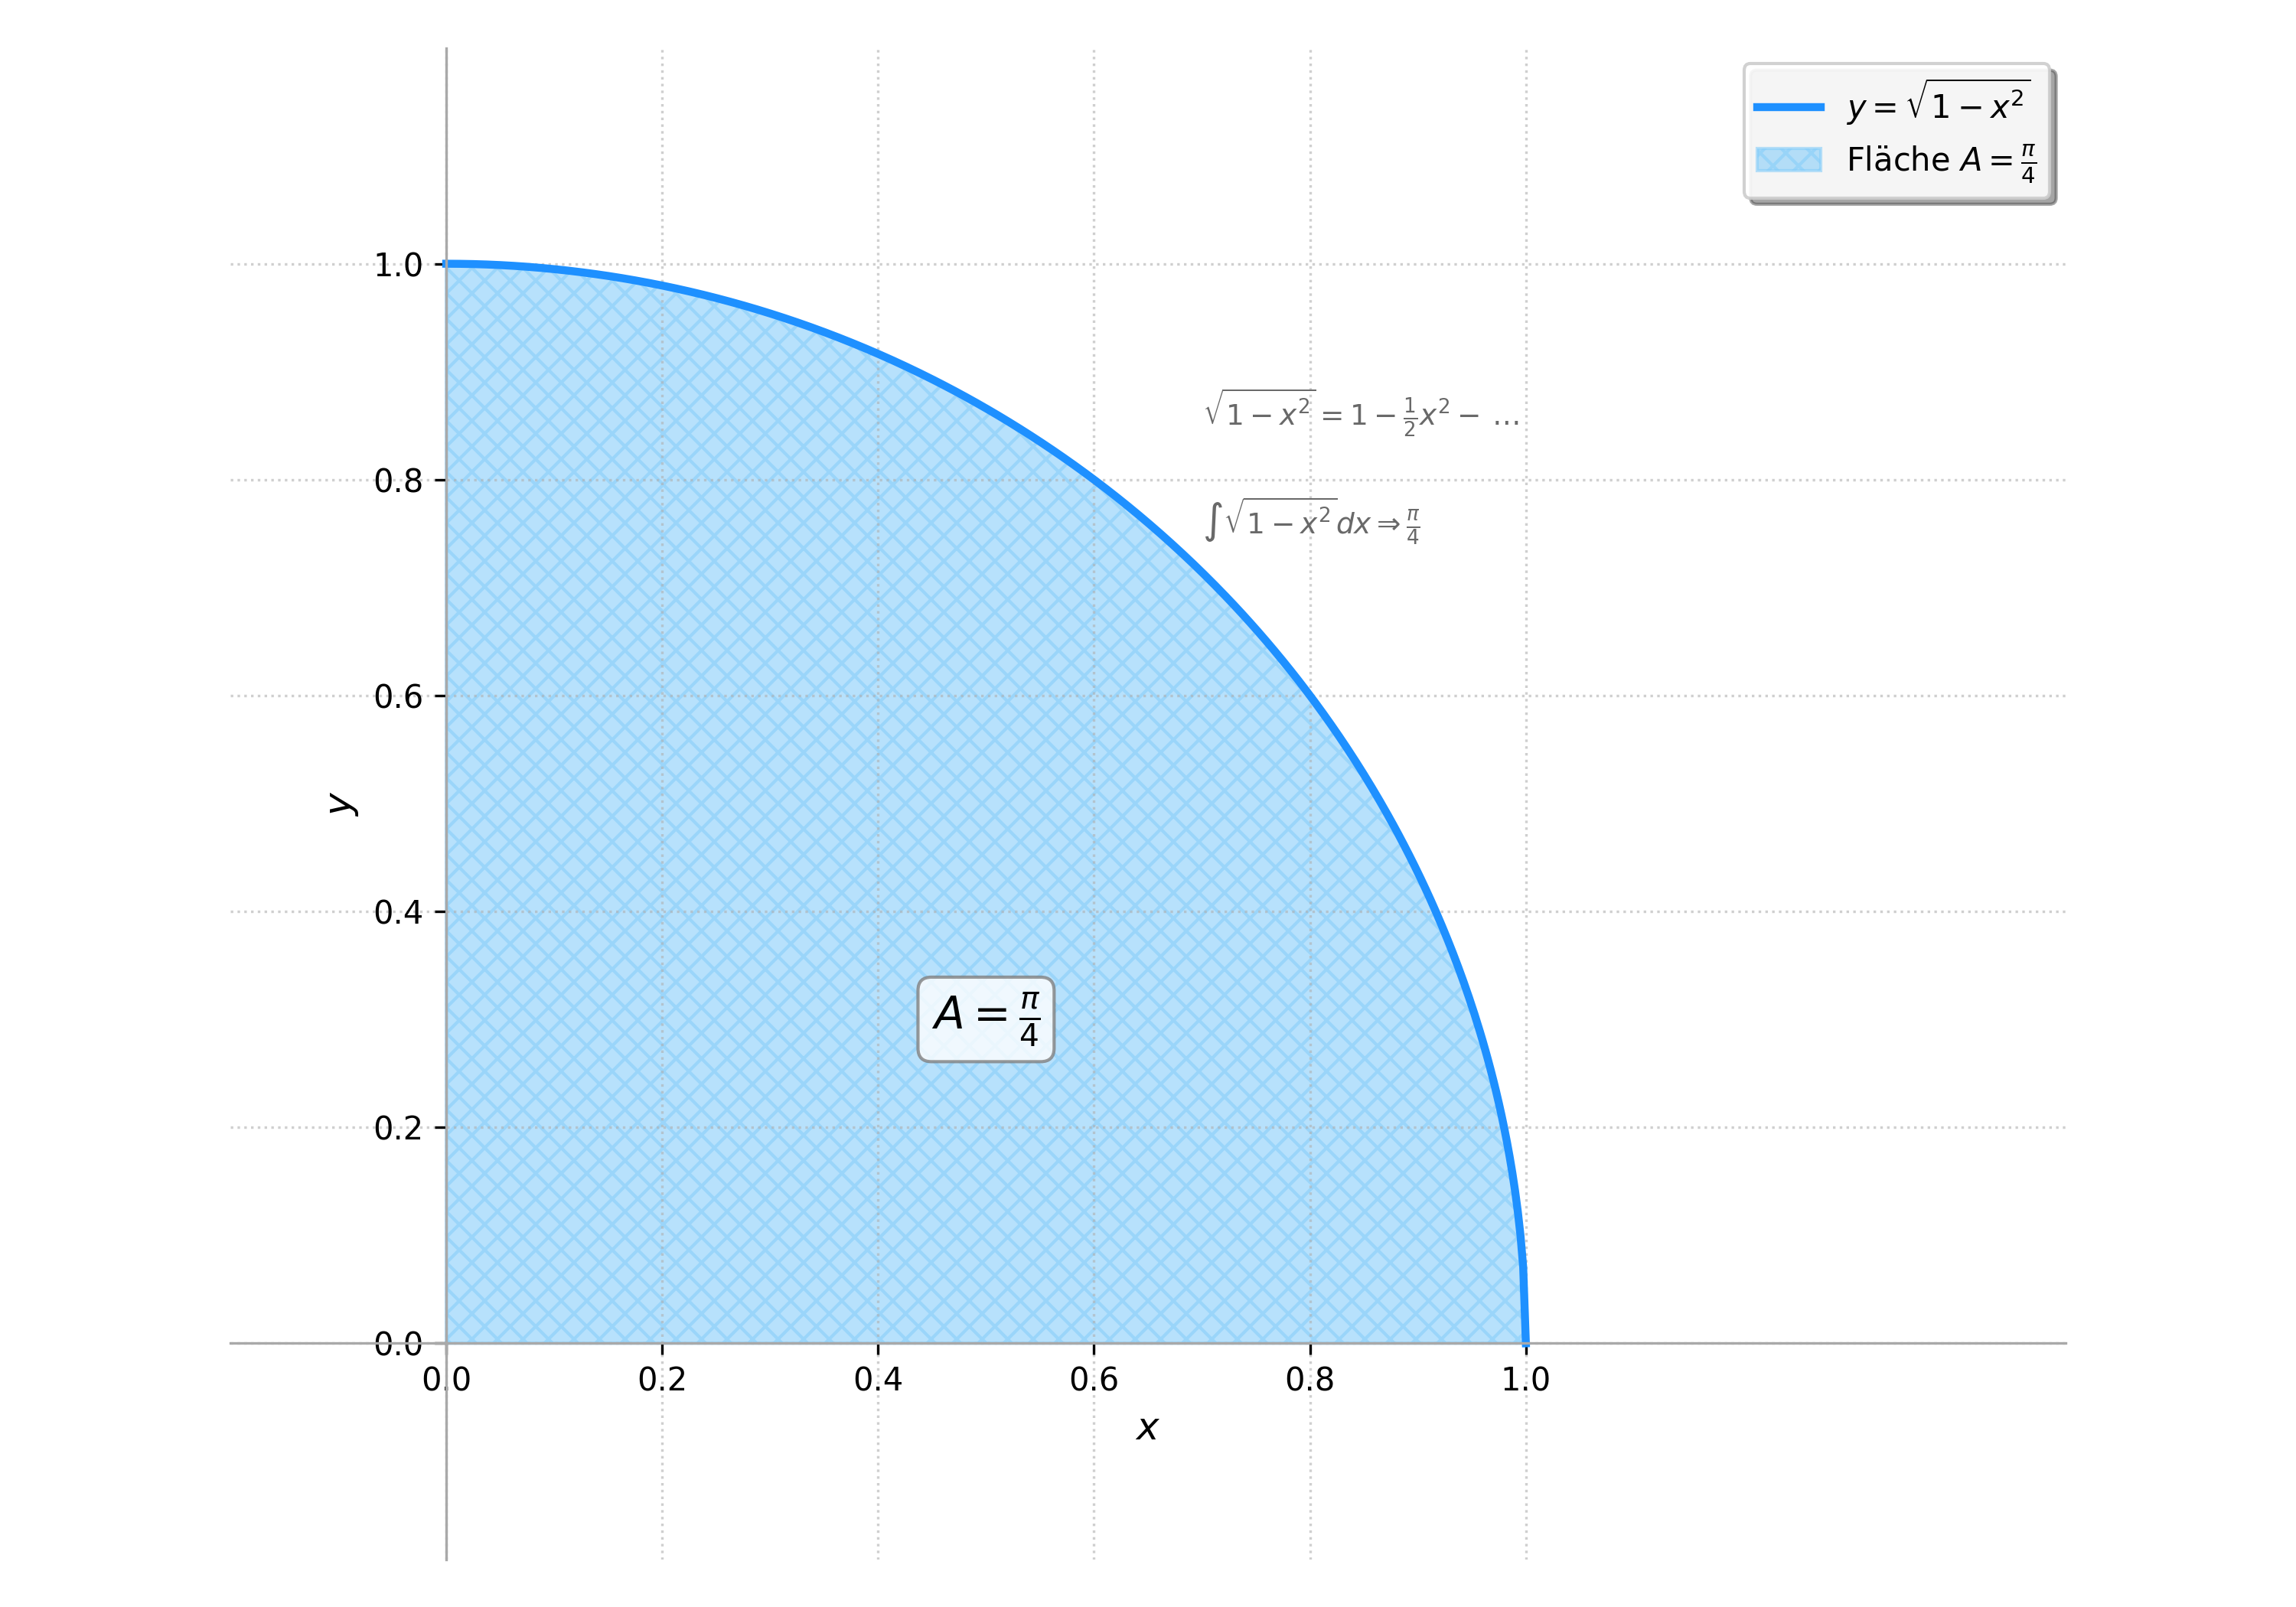
\includegraphics[width=0.6\textwidth]{grafiken/Newton_Pi_Integral.png}
    % Beschreibung für die Grafik 'Newton_Pi_Integral.png':
    % Die Grafik könnte den Graphen von y = sqrt(1-x^2) im ersten Quadranten zeigen (Viertelkreis).
    % Darunter die Fläche von x=0 bis x=1 schraffiert, beschriftet mit A = Pi/4.
    % Daneben oder darunter die ersten Terme der Reihe für sqrt(1-x^2) und 
    % die ersten Terme der integrierten Reihe für Pi/4.
    % Optional ein kleines Portrait von Newton.
    \captionof{figure}{Konzept der $\pi$-Berechnung durch Integration der Binomialreihe für den Viertelkreis}
    \label{fig:newton_pi_integral_funfact}
\end{center}
\end{funfactbox}

\subsubsection{Anwendungen und Interpretationen des bestimmten Integrals}

Die wichtigste geometrische Interpretation des bestimmten Integrals $\int_a^b f(x)dx$ ist, wie erwähnt, der orientierte Flächeninhalt zwischen dem Graphen von $f(x)$ und der x-Achse im Intervall $[a,b]$.

\begin{infoboxumgebung}{Flächenberechnung bei Nullstellen und unterhalb der x-Achse}
Wenn eine Funktion $f(x)$ im Integrationsintervall $[a,b]$ Nullstellen besitzt und somit Teile des Graphen unterhalb der x-Achse liegen, liefert das bestimmte Integral $\int_a^b f(x)dx$ die \textbf{Flächenbilanz}. Das bedeutet, Flächenstücke oberhalb der x-Achse werden positiv gewertet, Flächenstücke unterhalb der x-Achse negativ.

Um den \textbf{tatsächlichen geometrischen Flächeninhalt} zu berechnen, der zwischen dem Graphen und der x-Achse eingeschlossen wird, musst du:
\begin{enumerate}
    \item Die Nullstellen $x_N$ der Funktion im Intervall $[a,b]$ finden.
    \item Das Integral über die Teilintervalle berechnen, die durch die Nullstellen entstehen.
    \item Die \textbf{Beträge} der Integralteile addieren, bei denen der Graph unterhalb der x-Achse verläuft (also wo das Integral negativ wäre).
\end{enumerate}
Mathematisch entspricht das der Berechnung von $\int_a^b |f(x)| \,dx$. In der Praxis ist es oft einfacher, die Teilintegrale zu berechnen und dann die Beträge zu addieren.

Beispiel: Wenn $f(x)$ eine Nullstelle $x_N$ zwischen $a$ und $b$ hat und $f(x) \ge 0$ für $x \in [a, x_N]$ und $f(x) \le 0$ für $x \in [x_N, b]$, dann ist der Gesamtflächeninhalt $A_{ges}$:
\[ A_{ges} = \int_a^{x_N} f(x) \,dx + \left| \int_{x_N}^b f(x) \,dx \right| = \int_a^{x_N} f(x) \,dx - \int_{x_N}^b f(x) \,dx \]
(Da $\int_{x_N}^b f(x) \,dx$ negativ wäre, wird durch das Minuszeichen der Betrag addiert).
\end{infoboxumgebung}

\begin{beispielumgebung}{Fläche mit Anteilen unter der x-Achse}
Berechne den Flächeninhalt, den der Graph der Funktion $f(x) = x^2 - 1$ mit der x-Achse im Intervall $[-2, 2]$ einschließt.

\textbf{Schritt 1: Nullstellen von $f(x)$ finden.}
$x^2 - 1 = 0 \implies x^2 = 1 \implies x_{N1} = -1, x_{N2} = 1$.
Beide Nullstellen liegen im Intervall $[-2,2]$.

\textbf{Schritt 2: Vorzeichen von $f(x)$ in den Teilintervallen bestimmen.}
Die Parabel $f(x)=x^2-1$ ist nach oben geöffnet.
\begin{itemize}
    \item Intervall $[-2, -1]$: z.B. $f(-1.5) = (-1.5)^2-1 = 2.25-1 = 1.25 > 0$. (Graph oberhalb)
    \item Intervall $[-1, 1]$: z.B. $f(0) = 0^2-1 = -1 < 0$. (Graph unterhalb)
    \item Intervall $[1, 2]$: z.B. $f(1.5) = (1.5)^2-1 = 2.25-1 = 1.25 > 0$. (Graph oberhalb)
\end{itemize}

\textbf{Schritt 3: Teilintegrale berechnen.}
Stammfunktion $F(x) = \frac{1}{3}x^3 - x$.
$A_1 = \int_{-2}^{-1} (x^2-1) \,dx = [\frac{1}{3}x^3-x]_{-2}^{-1} = (\frac{1}{3}(-1)^3 - (-1)) - (\frac{1}{3}(-2)^3 - (-2))$
$= (-\frac{1}{3}+1) - (-\frac{8}{3}+2) = \frac{2}{3} - (-\frac{8}{3}+\frac{6}{3}) = \frac{2}{3} - (-\frac{2}{3}) = \frac{2}{3} + \frac{2}{3} = \frac{4}{3}$.

$A_2 = \int_{-1}^{1} (x^2-1) \,dx = [\frac{1}{3}x^3-x]_{-1}^{1} = (\frac{1}{3}(1)^3 - 1) - (\frac{1}{3}(-1)^3 - (-1))$
$= (\frac{1}{3}-1) - (-\frac{1}{3}+1) = -\frac{2}{3} - \frac{2}{3} = -\frac{4}{3}$.
(Das Integral ist negativ, da die Fläche unter der x-Achse liegt. Der Flächen\textit{inhalt} ist $|-\frac{4}{3}| = \frac{4}{3}$).

$A_3 = \int_{1}^{2} (x^2-1) \,dx = [\frac{1}{3}x^3-x]_{1}^{2} = (\frac{1}{3}(2)^3 - 2) - (\frac{1}{3}(1)^3 - 1)$
$= (\frac{8}{3}-2) - (\frac{1}{3}-1) = (\frac{8}{3}-\frac{6}{3}) - (-\frac{2}{3}) = \frac{2}{3} + \frac{2}{3} = \frac{4}{3}$.

\textbf{Schritt 4: Gesamtflächeninhalt.}
$A_{ges} = A_1 + |A_2| + A_3 = \frac{4}{3} + \frac{4}{3} + \frac{4}{3} = \frac{12}{3} = 4$.
Der Gesamtflächeninhalt beträgt 4 Flächeneinheiten.
\begin{center}
    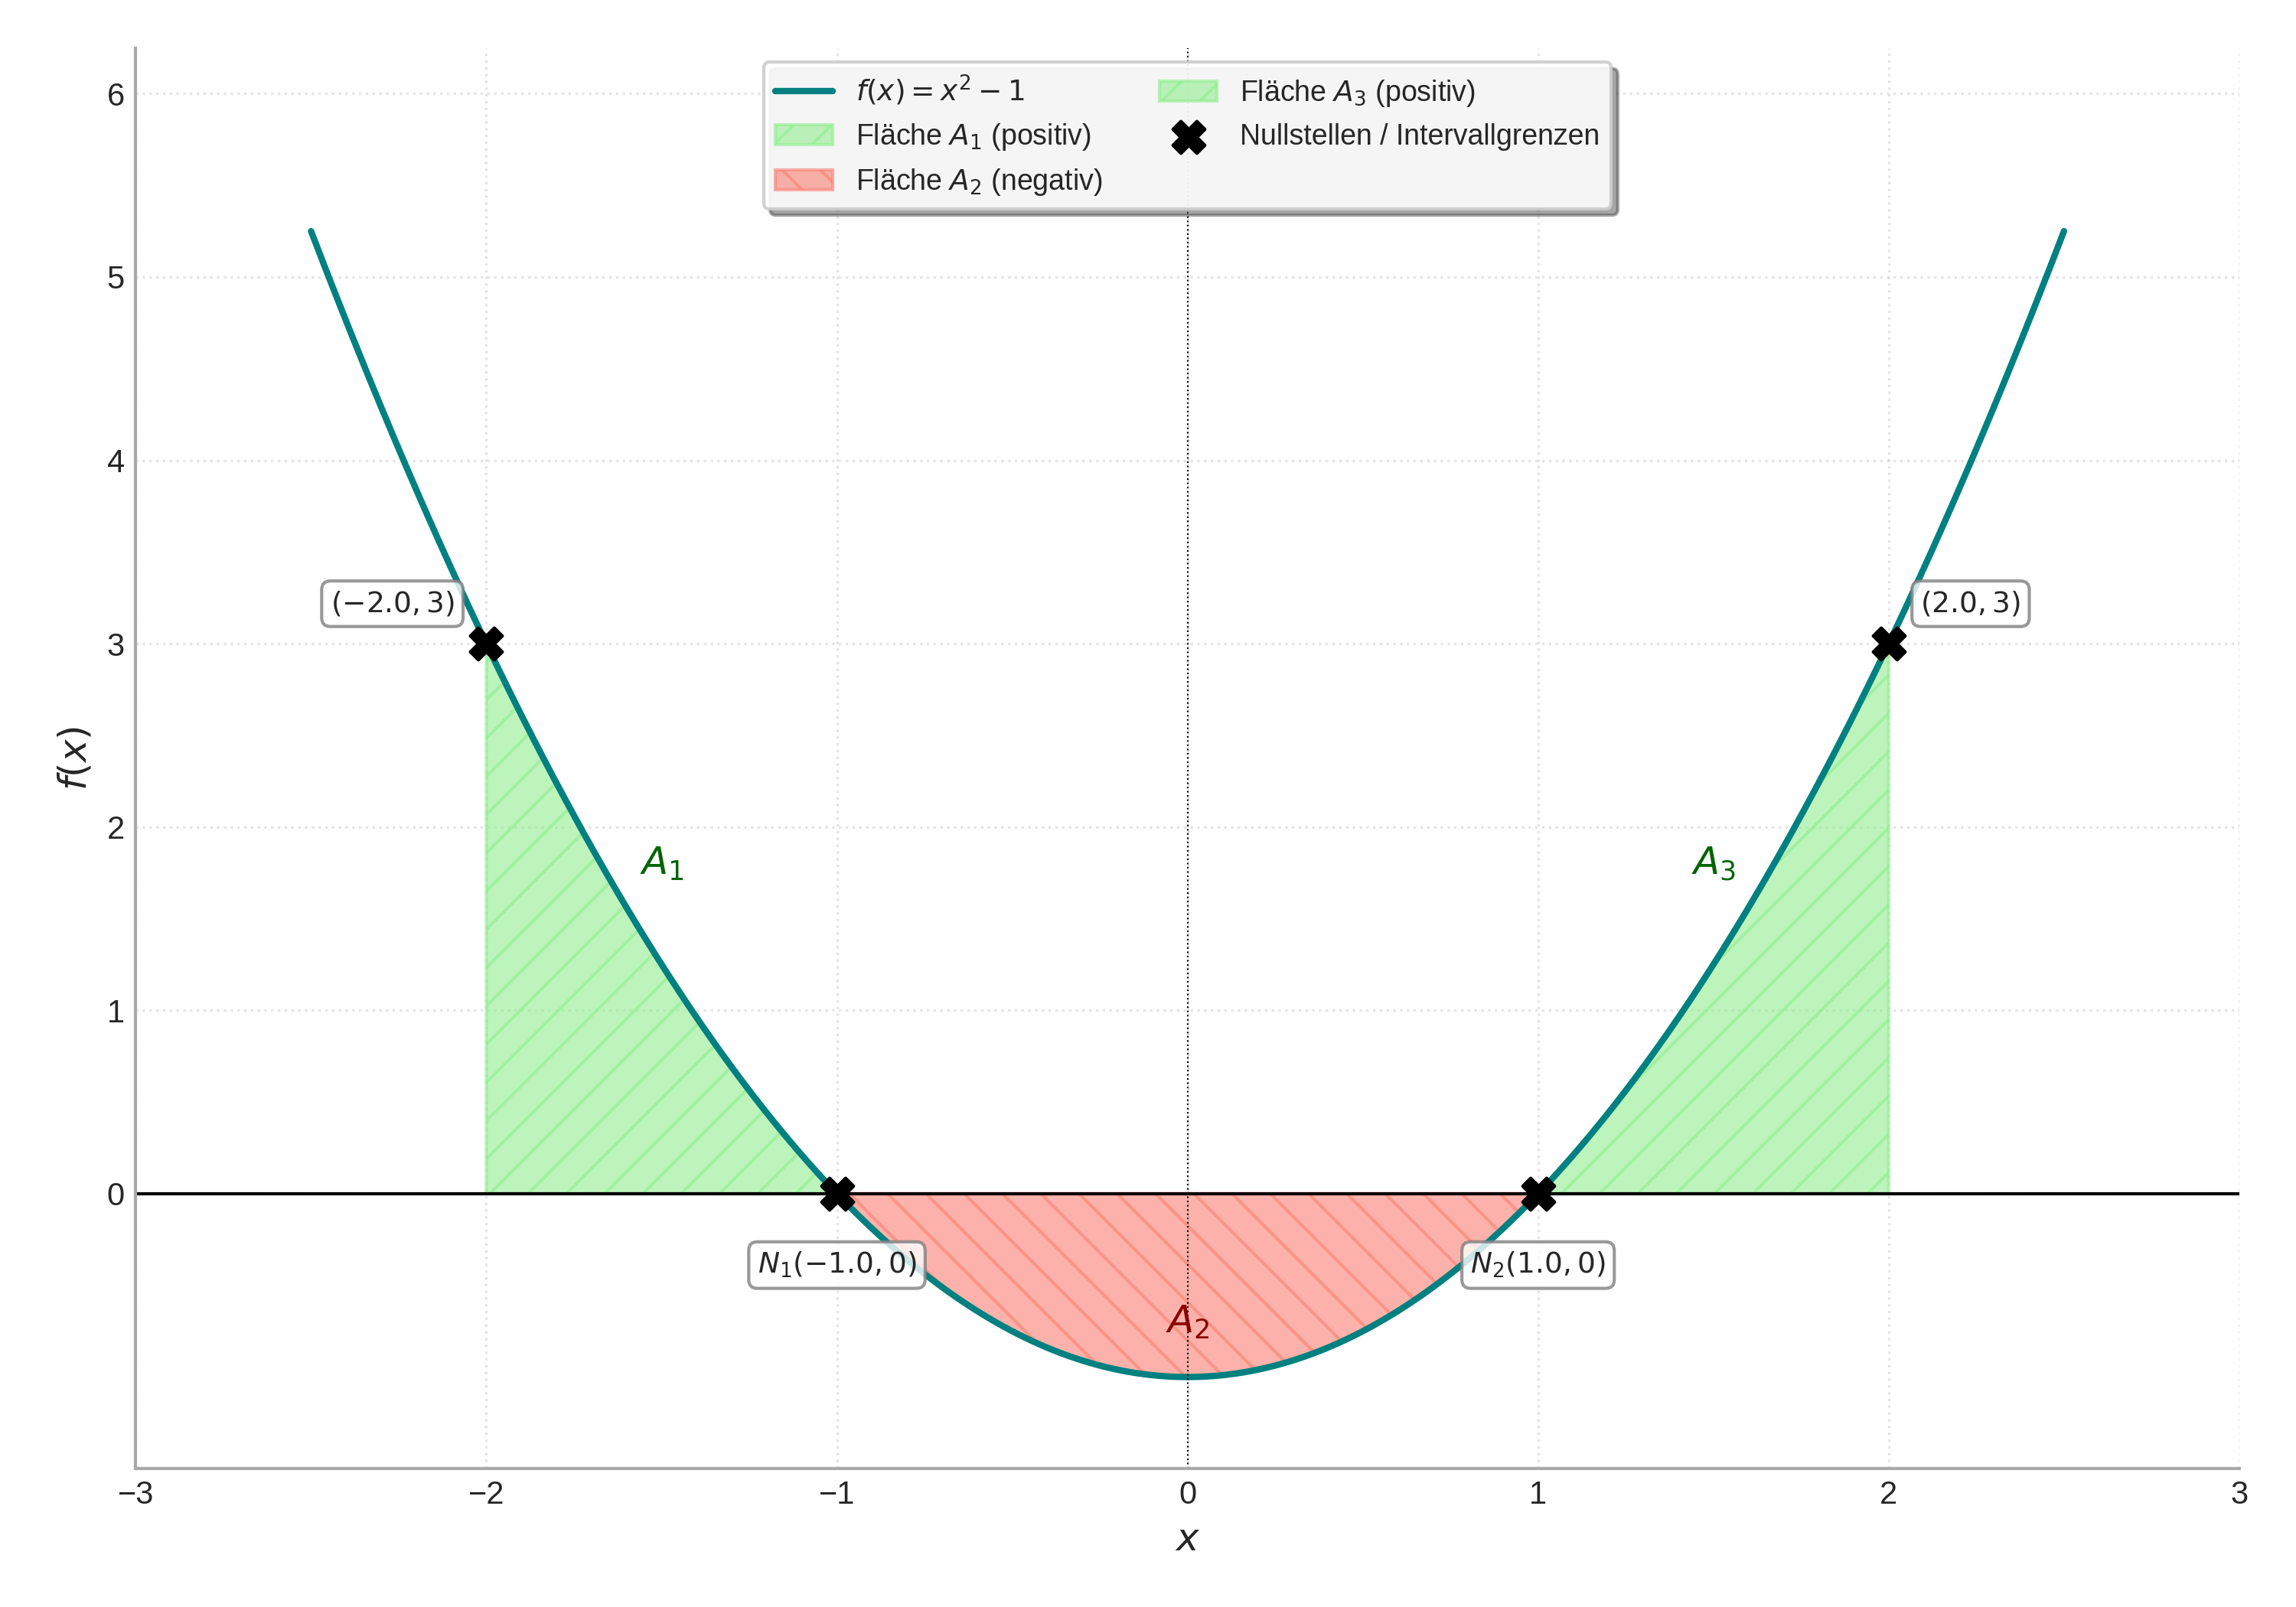
\includegraphics[width=0.8\textwidth]{grafiken/Integral_Flaeche_xhoch2minus1.png}
    \captionof{figure}{Fläche zwischen $f(x)=x^2-1$ und der x-Achse von -2 bis 2}
    \label{fig:flaeche_x2minus1}
\end{center}
\end{beispielumgebung}

\begin{aufgabenumgebung}{Flächenberechnung mit Nullstellen im Intervall}
Berechne den Inhalt der Fläche, die vom Graphen der Funktion $f(x) = x^3 - x$ und der x-Achse im Intervall $[-2, 2]$ eingeschlossen wird.
\begin{tippumgebung}{Vorgehen}
\begin{enumerate}
    \item Skizziere den Graphen (oder überlege dir den Verlauf anhand von Symmetrie und Nullstellen).
    \item Finde alle Nullstellen von $f(x)$.
    \item Bestimme, in welchen Teilintervallen $f(x) \ge 0$ und in welchen $f(x) \le 0$ ist.
    \item Berechne die bestimmten Integrale über die Teilintervalle und addiere deren Beträge.
\end{enumerate}
\end{tippumgebung}
\end{aufgabenumgebung}

\begin{infoboxumgebung}{Symmetrie und bestimmte Integrale – Rechnungen vereinfachen!}
Die Symmetrieeigenschaften von Funktionen können uns die Berechnung bestimmter Integrale oft erheblich erleichtern, besonders wenn das Integrationsintervall symmetrisch zum Ursprung ist (also von der Form $[-a, a]$).

\begin{itemize}
    \item \textbf{Punktsymmetrie zum Ursprung:}
        Wenn eine Funktion $f(x)$ punktsymmetrisch zum Ursprung ist (d.h. $f(-x) = -f(x)$, wie z.B. bei $x, x^3, x^5, \sin(x)$), dann gilt für jedes $a>0$:
        \[ \int_{-a}^{a} f(x) \,dx = 0 \]
        \textit{Warum?} Die Fläche links vom Ursprung (unterhalb der x-Achse, wenn $f(x)$ für $x>0$ oberhalb ist) ist genauso groß wie die Fläche rechts vom Ursprung (oberhalb der x-Achse), aber mit entgegengesetztem Vorzeichen. Sie heben sich also gegenseitig auf.
        \begin{center}
            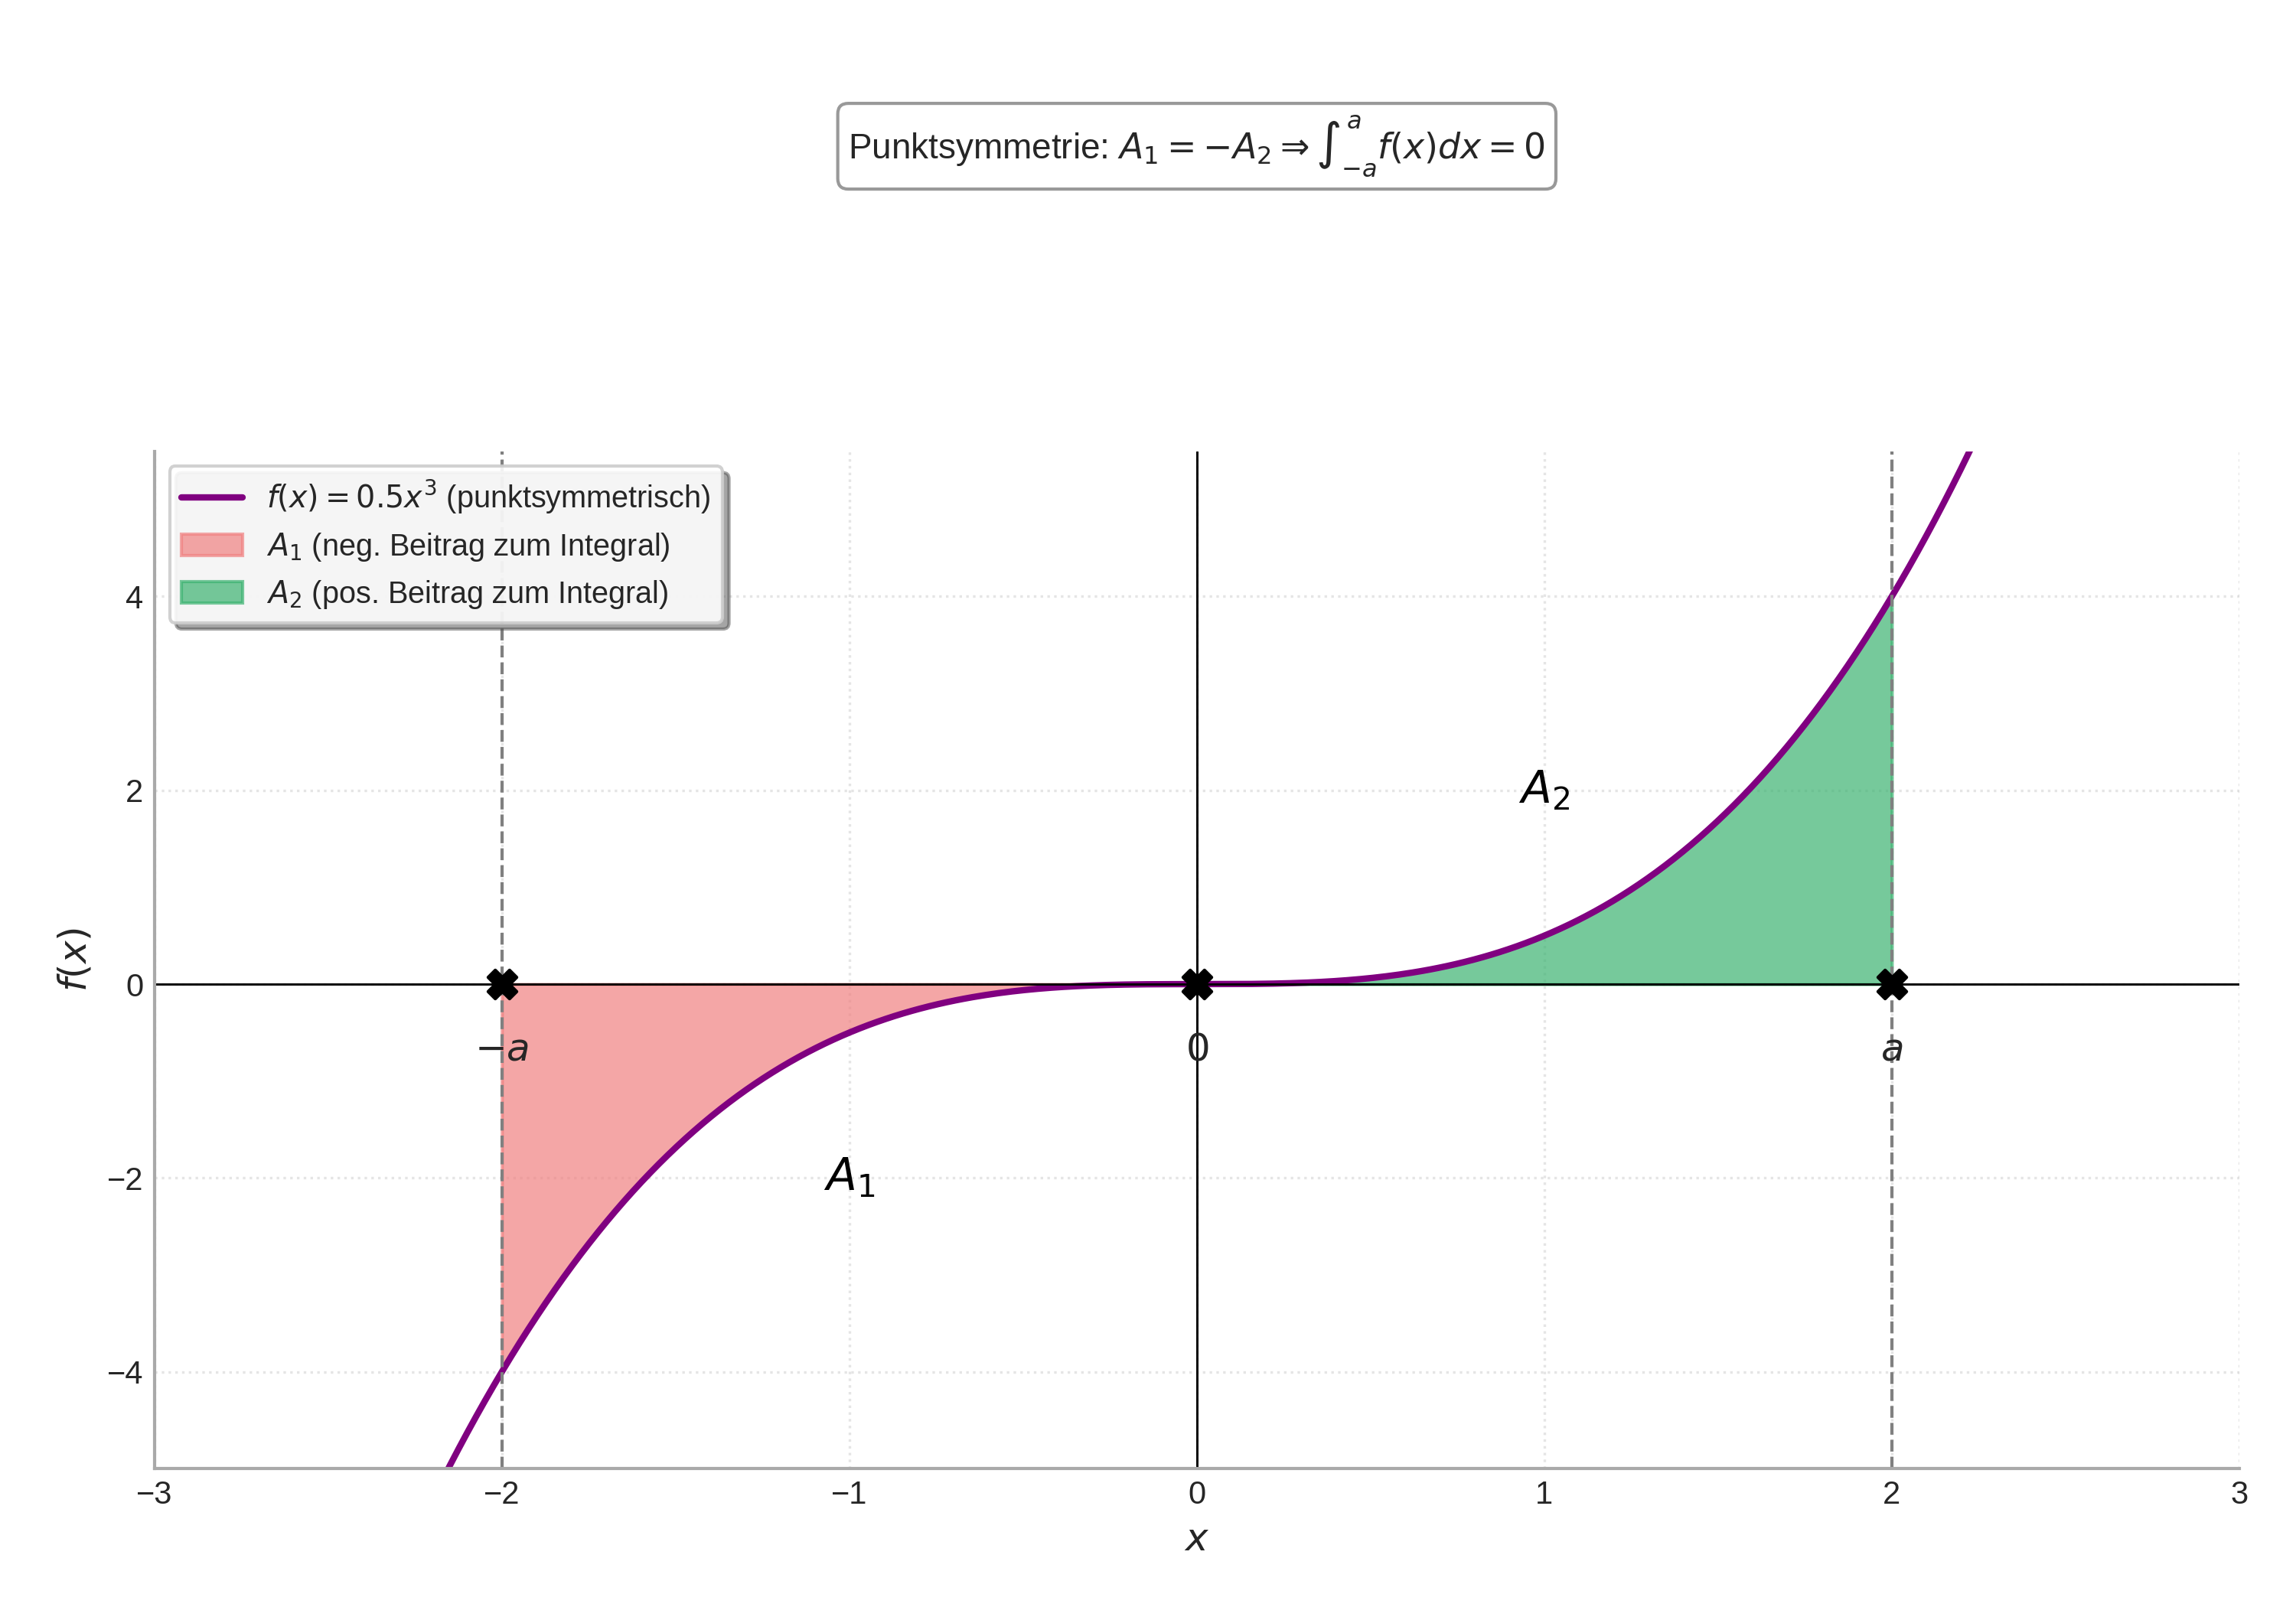
\includegraphics[width=0.7\textwidth]{grafiken/Integral_Punktsymmetrie.png}
            \captionof{figure}{Integral einer punktsymmetrischen Funktion über $[-a,a]$}
            \label{fig:integral_punktsymmetrie}
        \end{center}

    \item \textbf{Achsensymmetrie zur y-Achse:}
        Wenn eine Funktion $f(x)$ achsensymmetrisch zur y-Achse ist (d.h. $f(-x) = f(x)$, wie z.B. bei $x^2, x^4, |x|, \cos(x)$), dann gilt für jedes $a>0$:
        \[ \int_{-a}^{a} f(x) \,dx = 2 \cdot \int_{0}^{a} f(x) \,dx \]
        \textit{Warum?} Die Fläche links von der y-Achse (von $-a$ bis $0$) ist genauso groß wie die Fläche rechts von der y-Achse (von $0$ bis $a$). Man kann also die Rechnung vereinfachen, indem man nur eine Hälfte berechnet und das Ergebnis verdoppelt.
        % \begin{center}
        %     % Platzhalter für die Grafik 'Integral Achsensymmetrie'
        %     \framebox{\begin{minipage}{0.7\textwidth}
        %         \centering \vspace{1.5cm}
        %         \textbf{Platzhalter: Integral\_Achsensymmetrie.png} \\
        %         Beschreibung: Graph einer achsensymmetrischen Funktion (z.B. $x^2$) über $[-a,a]$. Die Fläche $A_1$ von $-a$ bis $0$ und $A_2$ von $0$ bis $a$ sind gleich groß und haben das gleiche Vorzeichen.
        %         \vspace{1.5cm}
        %     \end{minipage}}
        %     \captionof{figure}{Integral einer achsensymmetrischen Funktion über $[-a,a]$ (Platzhalter).}
        % \end{center}
        \begin{center}
            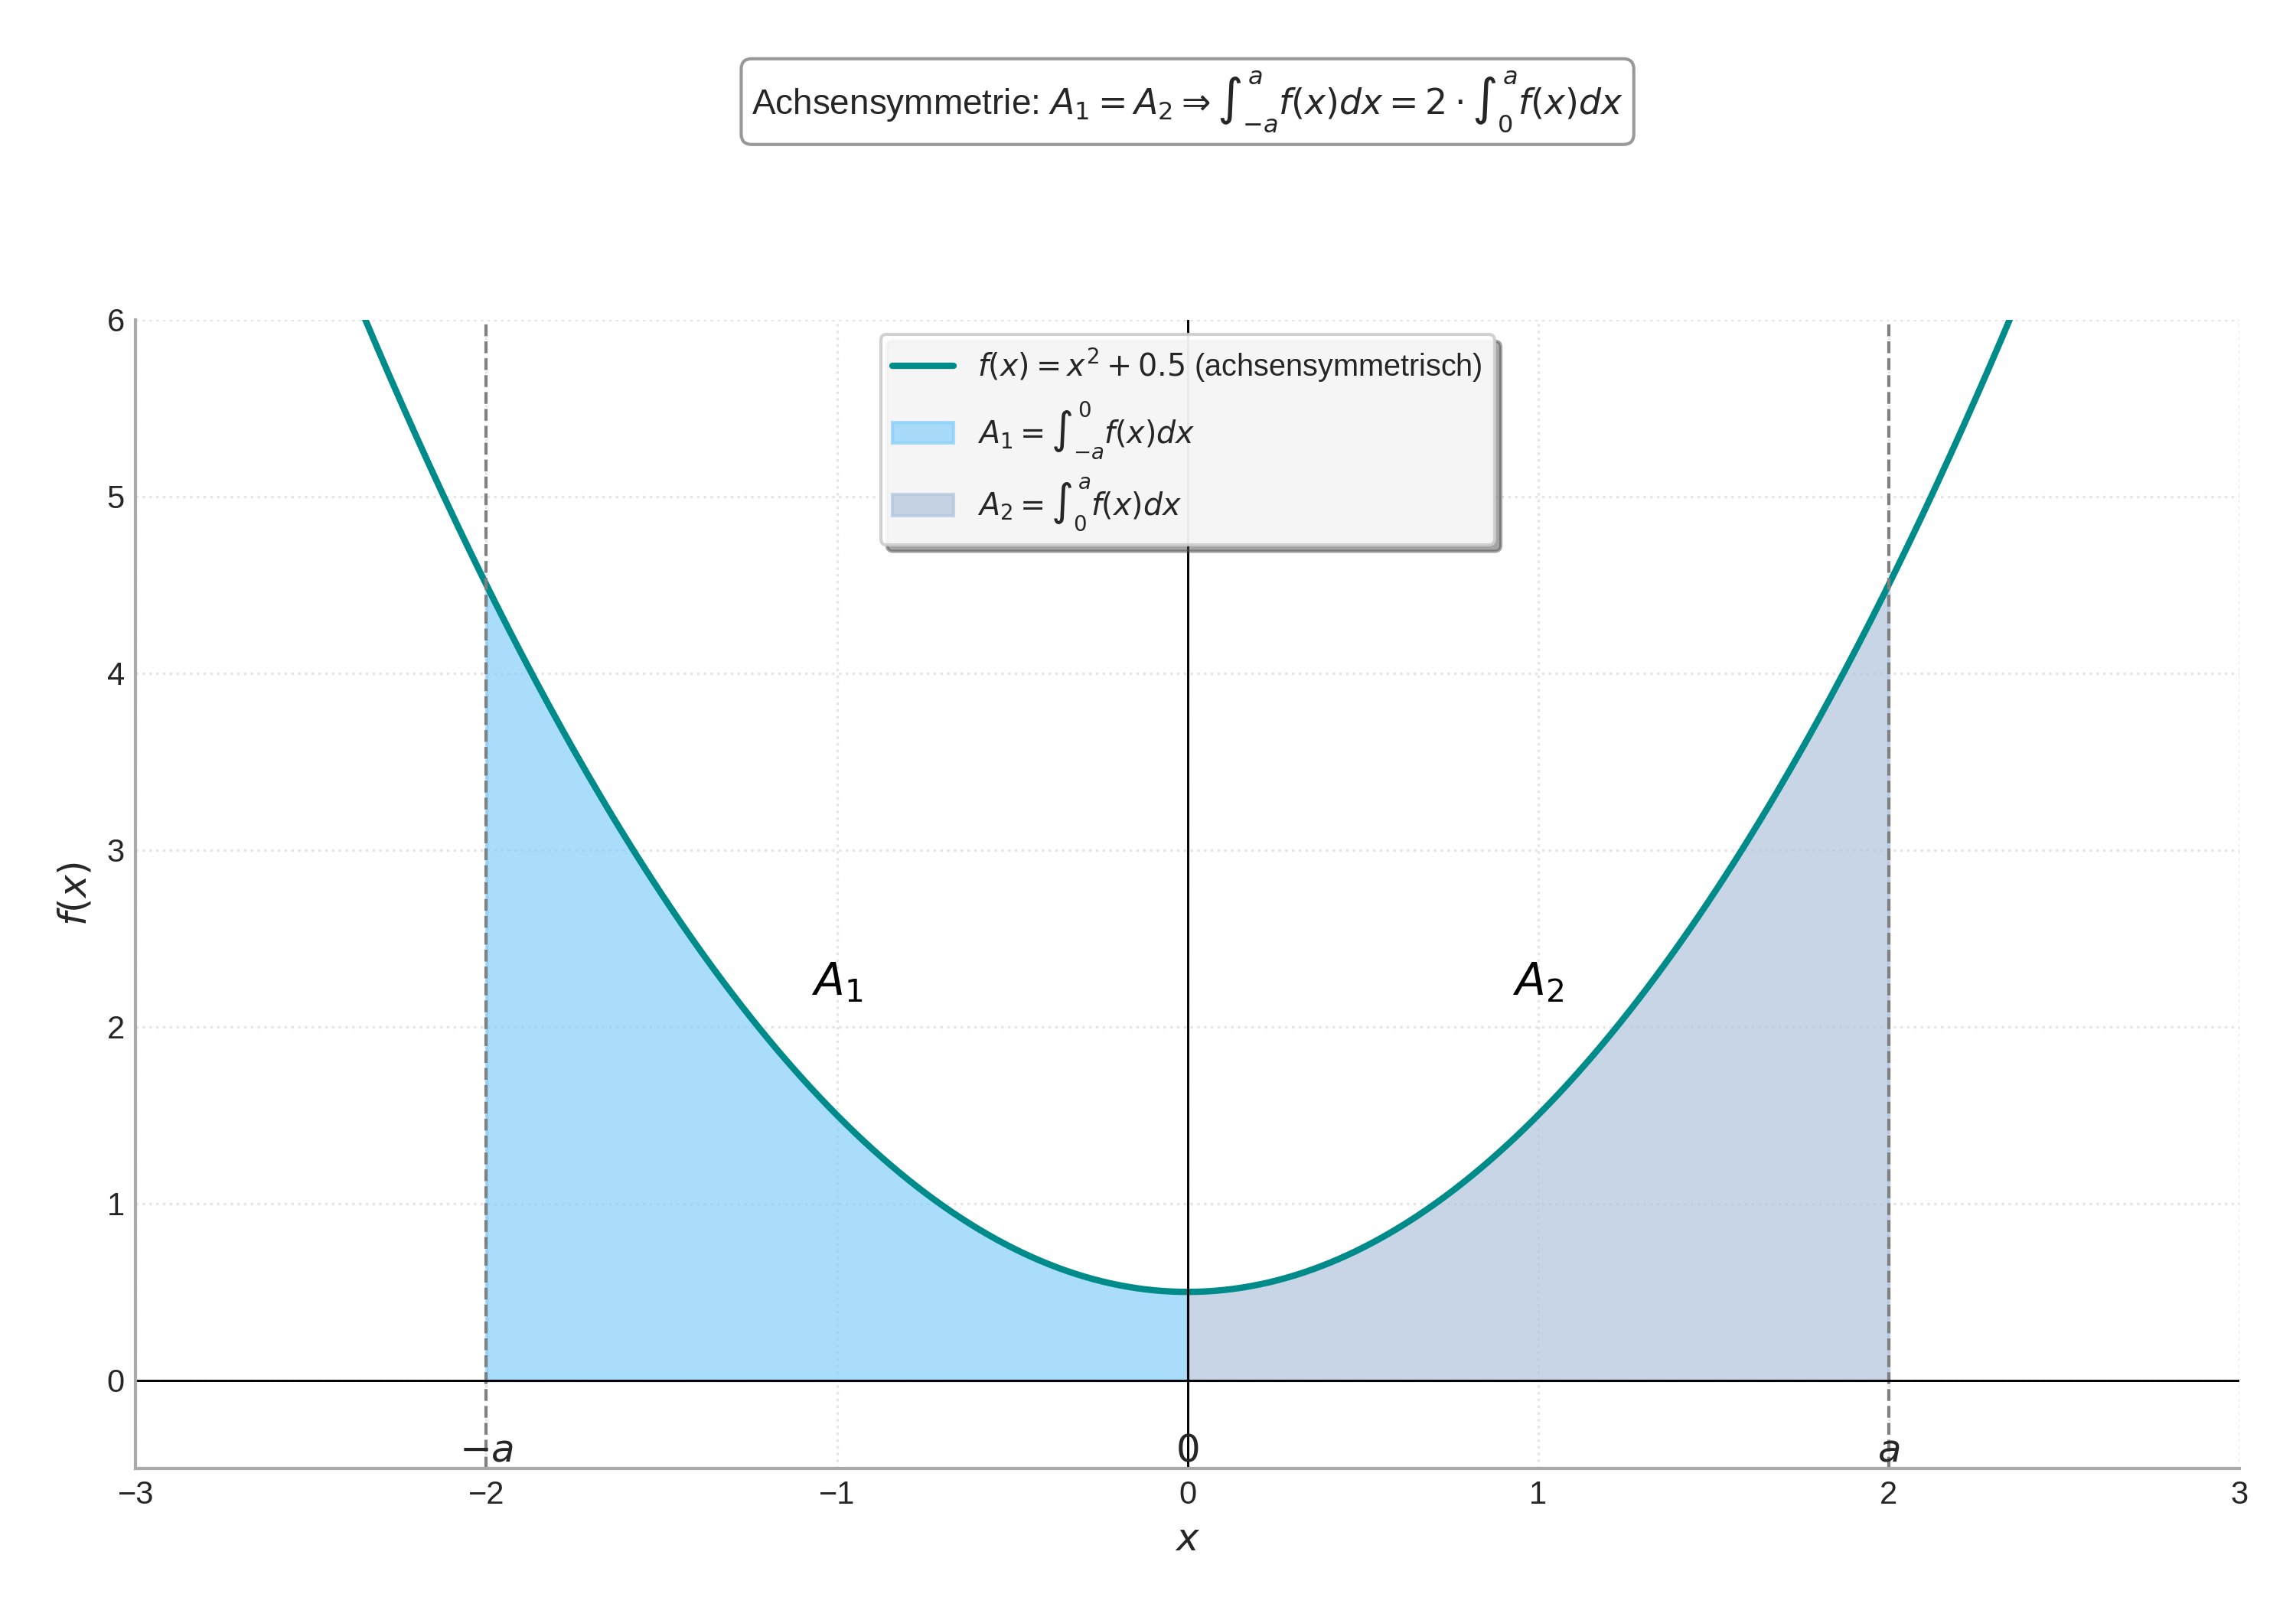
\includegraphics[width=0.7\textwidth]{grafiken/Integral_Achsensymmetrie.png}
            \captionof{figure}{Integral einer achsensymmetrischen Funktion über $[-a,a]$}
            \label{fig:integral_achsensymmetrie}
        \end{center}
\end{itemize}
Diese Symmetrieüberlegungen können dir viel Rechenarbeit ersparen!
\end{infoboxumgebung}

\begin{beispielumgebung}{Symmetrie beim Integrieren nutzen}
\begin{enumerate}
    \item Berechne $\int_{-1}^{1} x^3 \,dx$.
        Die Funktion $f(x)=x^3$ ist punktsymmetrisch zum Ursprung, da $f(-x)=(-x)^3 = -x^3 = -f(x)$.
        Das Integrationsintervall $[-1,1]$ ist symmetrisch zum Ursprung.
        Daher gilt: $\int_{-1}^{1} x^3 \,dx = 0$.
        \textit{Probe (mit HDI):} $F(x) = \frac{1}{4}x^4$.
        $[ \frac{1}{4}x^4 ]_{-1}^{1} = (\frac{1}{4}(1)^4) - (\frac{1}{4}(-1)^4) = \frac{1}{4} - \frac{1}{4} = 0$. Stimmt!

    \item Berechne $\int_{-2}^{2} (3x^2 - 5) \,dx$.
        Die Funktion $f(x)=3x^2-5$ ist achsensymmetrisch zur y-Achse, da sie nur gerade Potenzen von $x$ enthält (und eine Konstante): $f(-x) = 3(-x)^2-5 = 3x^2-5 = f(x)$.
        Das Intervall $[-2,2]$ ist symmetrisch.
        Daher: $\int_{-2}^{2} (3x^2 - 5) \,dx = 2 \cdot \int_{0}^{2} (3x^2 - 5) \,dx$.
        Stammfunktion $F(x) = x^3 - 5x$.
        $2 \cdot [x^3 - 5x]_{0}^{2} = 2 \cdot ( ( (2)^3 - 5(2) ) - ( (0)^3 - 5(0) ) )$
        $= 2 \cdot ( (8 - 10) - (0) ) = 2 \cdot (-2) = -4$.
\end{enumerate}
\end{beispielumgebung}

\begin{aufgabenumgebung}{Symmetrie beim Integrieren anwenden}
Berechne die folgenden bestimmten Integrale. Nutze Symmetrieeigenschaften, wenn möglich, um die Rechnung zu vereinfachen.
\begin{enumerate}
    \item $\int_{-5}^{5} (x^5 - 2x^3 + x) \,dx$
    \item $\int_{-1}^{1} (x^4 + 3x^2 - 1) \,dx$
    \item $\int_{-\pi}^{\pi} \sin(x) \,dx$ (Du weißt vielleicht schon, dass $\sin(x)$ punktsymmetrisch ist. Die Stammfunktion von $\sin(x)$ ist $-\cos(x)$.)
\end{enumerate}
\end{aufgabenumgebung}

% Hier geht es dann weiter mit weiteren Anwendungen oder dem Abschluss des Kapitels.

% Vorheriger Inhalt des Kapitels bis zur aufgabenumgebung 'Symmetrie beim Integrieren anwenden'
% ... (siehe vorherige Canvas-Version) ...

\begin{aufgabenumgebung}{Fläche zwischen zwei Kurven}
Die Graphen der Funktionen $f(x) = -x^2 + 4x + 1$ und $g(x) = x^2 - 2x + 1$ schließen eine Fläche ein.
\begin{enumerate}
    \item \textbf{Schnittpunkte bestimmen:} Berechne die x-Koordinaten der Schnittpunkte der beiden Graphen, indem du $f(x) = g(x)$ setzt und die entstehende Gleichung löst. Diese Schnittpunkte sind deine Integrationsgrenzen $a$ und $b$.
    \item \textbf{Welche Funktion liegt oben?} Bestimme, welche der beiden Funktionen im Intervall $[a,b]$ die größeren Funktionswerte hat (also 'oben' liegt). Du kannst dies tun, indem du einen Testwert aus dem Intervall $(a,b)$ in beide Funktionen einsetzt oder die Graphen skizzierst.
    \item \textbf{Differenzfunktion bilden:} Bilde die Differenzfunktion $d(x) = \text{obere Funktion} - \text{untere Funktion}$.
    \item \textbf{Flächeninhalt berechnen:} Berechne den Flächeninhalt $A = \int_a^b d(x) \,dx$.
    \item \textbf{Skizze:} Skizziere beide Parabeln und die eingeschlossene Fläche in ein Koordinatensystem.
\end{enumerate}
\begin{merksatzumgebung}{Fläche zwischen zwei Graphen}
Den Flächeninhalt $A$ zwischen den Graphen zweier Funktionen $f(x)$ und $g(x)$ im Intervall $[a,b]$, wobei $f(x) \ge g(x)$ für alle $x \in [a,b]$ gilt (d.h. $f(x)$ ist die obere Funktion), berechnet man mit:
\[ A = \int_a^b (f(x) - g(x)) \,dx \]
Wenn nicht klar ist, welche Funktion oben liegt, oder wenn sich die obere Funktion ändert, muss man das Intervall entsprechend aufteilen und/oder den Betrag der Differenz integrieren: $A = \int_a^b |f(x) - g(x)| \,dx$.
\end{merksatzumgebung}
\begin{center}
    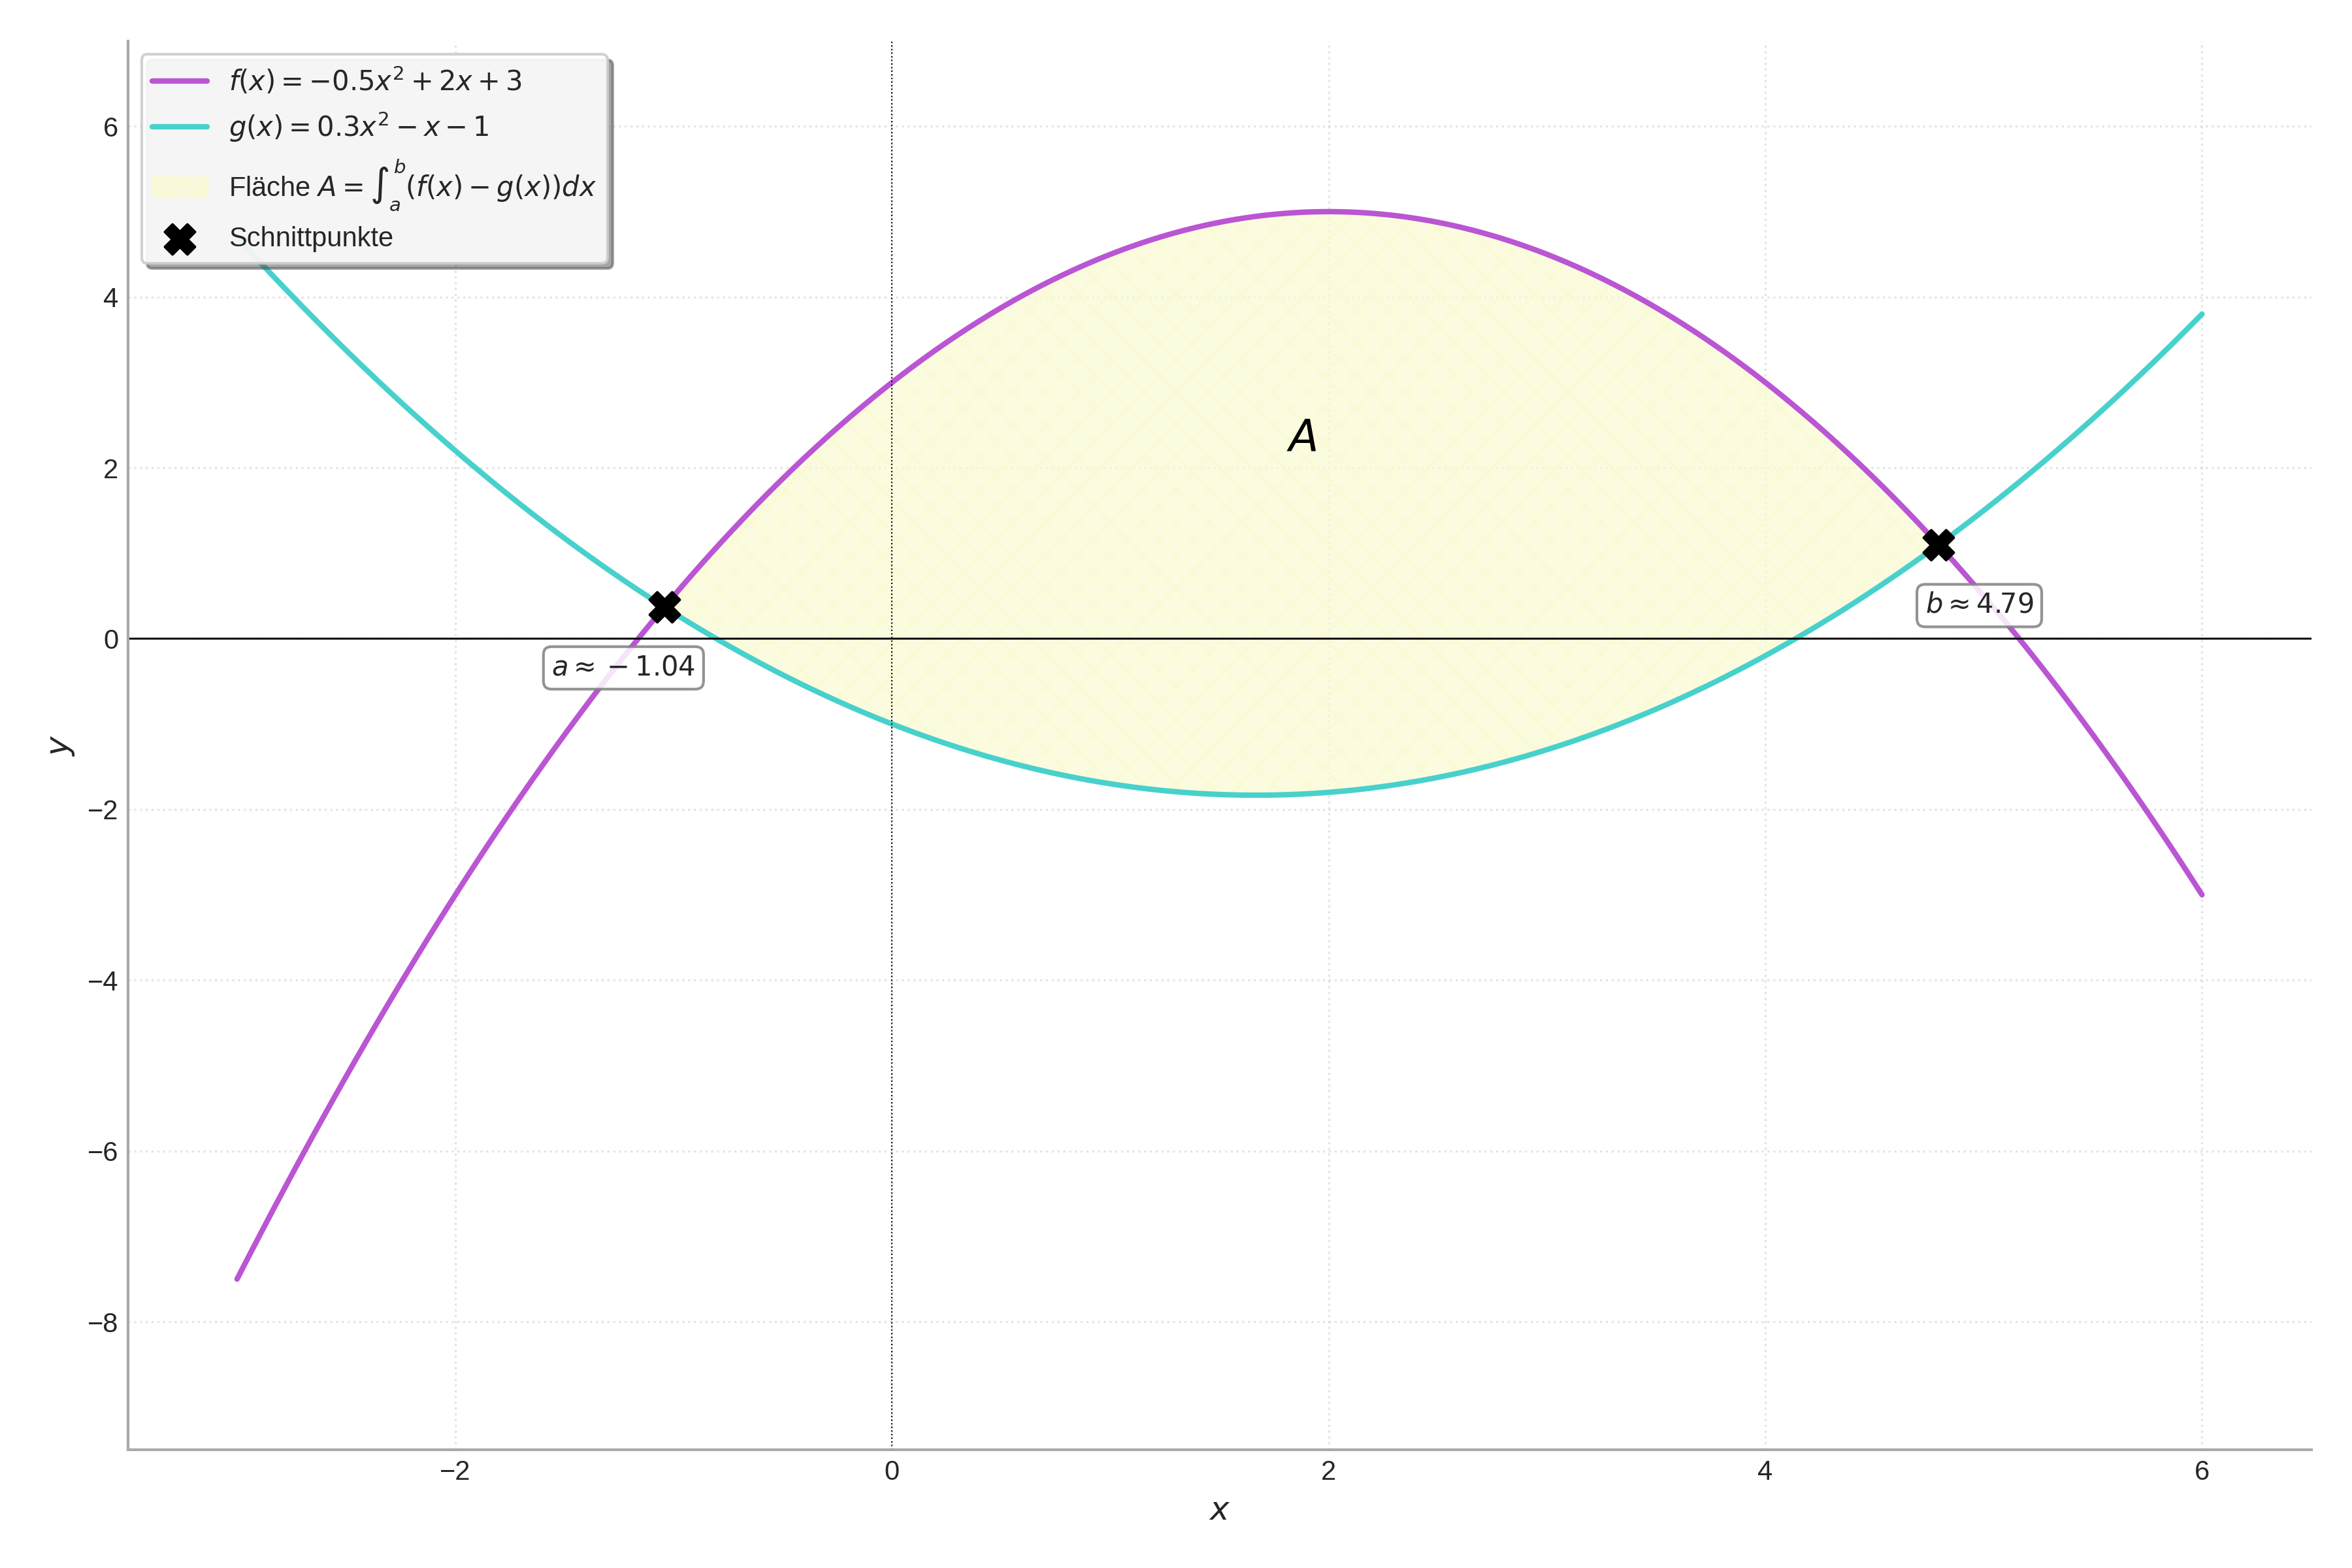
\includegraphics[width=0.8\textwidth]{grafiken/Integral_Flaeche_zwischen_Kurven.png}
    \captionof{figure}{Fläche zwischen den Graphen von $f(x)$ und $g(x)$}
    \label{fig:flaeche_zwischen_kurven}
\end{center}
\end{aufgabenumgebung}

\begin{aufgabenumgebung}{Der Mittelwert einer Funktion}
Manchmal möchte man nicht den Gesamtwert (wie die Gesamtfläche oder den Gesamtweg), sondern einen Durchschnittswert einer Größe über ein Intervall bestimmen. Die Integralrechnung hilft auch hier!

\begin{merksatzumgebung}{Mittelwert einer Funktion}
Der \textbf{Mittelwert $\mu$} einer stetigen Funktion $f(x)$ im Intervall $[a,b]$ (mit $a<b$) ist definiert als:
\[ \mu = \frac{1}{b-a} \int_a^b f(x) \,dx \]
\textit{Anschauliche Deutung:} Der Mittelwert $\mu$ ist die Höhe eines Rechtecks mit der Breite $(b-a)$, dessen Flächeninhalt gleich dem Flächeninhalt unter dem Graphen von $f(x)$ im Intervall $[a,b]$ ist. Also: $\mu \cdot (b-a) = \int_a^b f(x) \,dx$.
\end{merksatzumgebung}

\textbf{Aufgabe:}
Ein Tag hat vereinfacht 12 Stunden Helligkeit (von $t=0$ bis $t=12$). Die Temperatur $T$ (in °C) an diesem Tag kann durch die Funktion $T(t) = -0.5t^2 + 6t + 5$ modelliert werden.
\begin{enumerate}
    \item Skizziere den Graphen der Temperaturfunktion im Intervall $[0,12]$.
    \item Berechne die Durchschnittstemperatur während dieser 12 Stunden mit der Formel für den Mittelwert einer Funktion.
    \item Zeichne in deine Skizze ein Rechteck mit der Breite des Intervalls (12 Stunden) und der Höhe der Durchschnittstemperatur. Vergleiche die Fläche dieses Rechtecks mit der Fläche unter dem Temperatur-Graphen (visuell).
\end{enumerate}
\begin{center}
    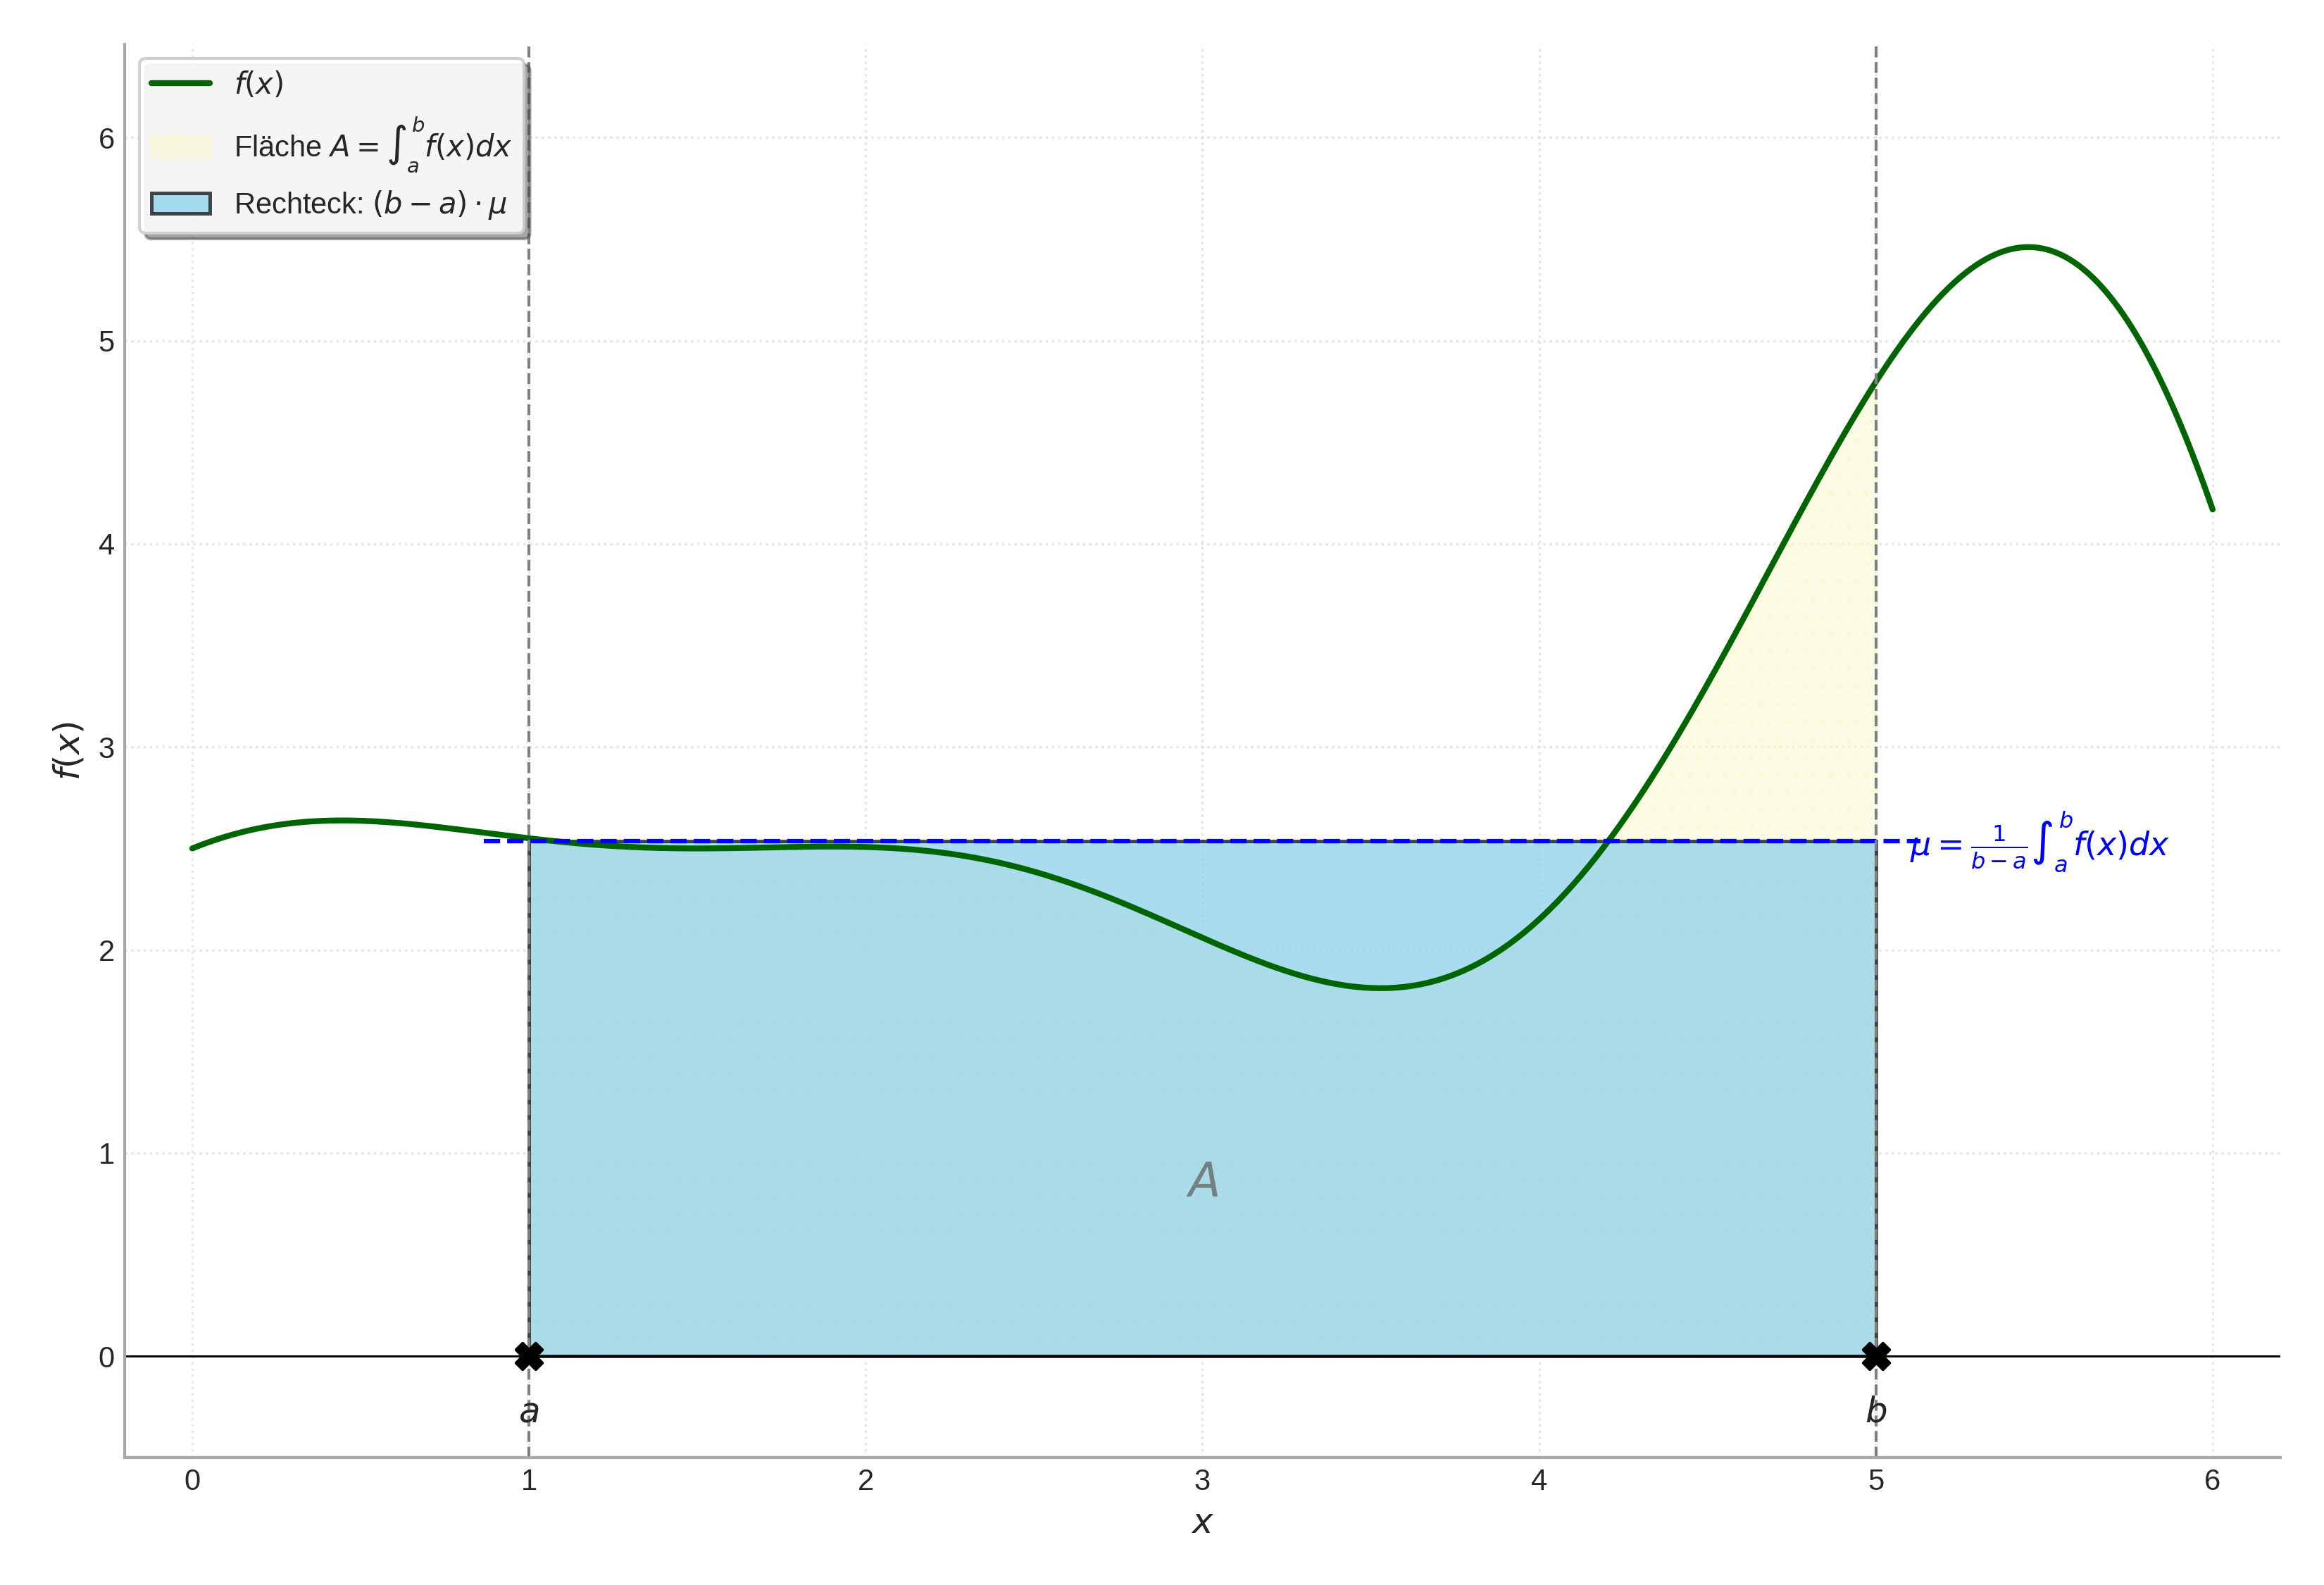
\includegraphics[width=0.8\textwidth]{grafiken/Integral_Mittelwert_Funktion.png}
    \captionof{figure}{Geometrische Deutung des Mittelwerts einer Funktion}
    \label{fig:mittelwert_funktion}
\end{center}
\end{aufgabenumgebung}

\begin{kurzknappumgebung}{Bestimmtes Integral und Hauptsatz}
\begin{itemize}
    \item \textbf{Bestimmtes Integral $\int_a^b f(x)dx$:} Grenzwert der Riemannsummen; gibt den orientierten Flächeninhalt zwischen Graph von $f(x)$ und x-Achse im Intervall $[a,b]$ an.
    \item \textbf{Stammfunktion $F(x)$:} Eine Funktion, deren Ableitung $f(x)$ ist ($F'(x)=f(x)$). Es gibt unendlich viele, die sich durch eine Konstante $C$ unterscheiden: $\int f(x)dx = F(x)+C$ (unbestimmtes Integral).
    \item \textbf{Hauptsatz (HDI):} $\int_a^b f(x)dx = F(b) - F(a)$. Ermöglicht einfache Berechnung bestimmter Integrale über Stammfunktionen.
    \item \textbf{Flächenberechnung:} Bei Nullstellen im Intervall müssen Teilintegrale gebildet und Beträge addiert werden für den geometrischen Flächeninhalt.
    \item \textbf{Symmetrie nutzen:} Bei punktsymmetrischen Funktionen über $[-a,a]$ ist $\int_{-a}^a f(x)dx = 0$. Bei achsensymmetrischen ist $\int_{-a}^a f(x)dx = 2 \cdot \int_0^a f(x)dx$.
    \item \textbf{Fläche zwischen Kurven $f(x)$ und $g(x)$ (mit $f(x) \ge g(x)$):} $A = \int_a^b (f(x)-g(x))dx$.
    \item \textbf{Mittelwert $\mu$ von $f(x)$ auf $[a,b]$:} $\mu = \frac{1}{b-a}\int_a^b f(x)dx$.
\end{itemize}
\end{kurzknappumgebung}

% Vorheriger Inhalt des Kapitels bis zur aufgabenumgebung 'Der Mittelwert einer Funktion'
% ... (siehe vorherige Canvas-Version) ...

\subsection{Zusammenfassung und Ausblick zur Integralrechnung}
\label{subsec:zusammenfassung_ausblick_integral}

Wir haben nun die fundamentalen Ideen der Integralrechnung kennengelernt: von der anschaulichen Flächenapproximation durch Riemannsummen über das Konzept der Stammfunktion als 'Gegenstück' zur Ableitung bis hin zum mächtigen Hauptsatz der Differential- und Integralrechnung. Mit diesen Werkzeugen können wir bereits viele wichtige Probleme lösen, insbesondere Flächeninhalte unter und zwischen Kurven von Polynomfunktionen berechnen sowie Mittelwerte von Funktionen bestimmen.

\begin{kurzknappumgebung}{Integralrechnung – Das Wichtigste auf einen Blick}
\begin{itemize}
    \item \textbf{Riemannsummen (Unter-/Obersumme):} Annäherung von Flächen unter Kurven durch Summen von Rechtecksflächen.
    \item \textbf{Bestimmtes Integral $\int_a^b f(x)dx$:} Grenzwert der Riemannsummen; gibt den orientierten Flächeninhalt zwischen dem Graphen von $f(x)$ und der x-Achse im Intervall $[a,b]$ an.
    \item \textbf{Stammfunktion $F(x)$:} Eine Funktion, deren Ableitung $f(x)$ ist ($F'(x)=f(x)$). Es gibt unendlich viele Stammfunktionen, die sich durch eine additive Konstante $C$ unterscheiden: $\int f(x)dx = F(x)+C$ (unbestimmtes Integral).
    \item \textbf{Hauptsatz der Differential- und Integralrechnung (HDI):} Die Brücke zwischen Ableiten und Integrieren!
    \[ \int_a^b f(x)dx = [F(x)]_a^b = F(b) - F(a) \]
    Er ermöglicht die exakte Berechnung bestimmter Integrale über Stammfunktionen.
    \item \textbf{Flächenberechnung:}
        \begin{itemize}
            \item Liegt $f(x)$ im Intervall $[a,b]$ nicht unterhalb der x-Achse, ist $A = \int_a^b f(x)dx$.
            \item Bei Nullstellen im Intervall müssen Teilintegrale gebildet und deren Beträge addiert werden, um den geometrischen Gesamtflächeninhalt zu erhalten ($A = \int_a^b |f(x)|dx$).
            \item Fläche zwischen zwei Kurven $f(x)$ und $g(x)$ (mit $f(x) \ge g(x)$ auf $[a,b]$): $A = \int_a^b (f(x)-g(x))dx$.
        \end{itemize}
    \item \textbf{Symmetrie nutzen:} Bei punktsymmetrischen Funktionen über $[-a,a]$ ist $\int_{-a}^a f(x)dx = 0$. Bei achsensymmetrischen ist $\int_{-a}^a f(x)dx = 2 \cdot \int_0^a f(x)dx$.
    \item \textbf{Mittelwert $\mu$ von $f(x)$ auf $[a,b]$:} $\mu = \frac{1}{b-a}\int_a^b f(x)dx$.
\end{itemize}
\end{kurzknappumgebung}

\begin{infoboxumgebung}{Ausblick: Was kommt noch in der Integralrechnung?}
Die bisher gelernten Integrationsregeln (Potenz-, Faktor-, Summenregel als Umkehrung der Ableitungsregeln) reichen für Polynomfunktionen und einfache gebrochen-rationale Funktionen gut aus. Aber was ist mit komplexeren Funktionen, die wir bereits beim Ableiten kennengelernt haben?
\begin{itemize}
    \item Wie integriert man Produkte von Funktionen, z.B. $f(x) = x^2 \cdot e^x$?
    \item Wie integriert man Quotienten, z.B. $g(x) = \frac{2x}{x^2+1}$?
    \item Wie integriert man verkettete Funktionen, z.B. $h(x) = (3x+5)^4$ oder $k(x) = e^{x^2+x+1} \cdot (2x+1)$ oder $m(x) = x \cdot \sin(x^2)$?
\end{itemize}
Für solche Fälle gibt es weiterführende \textbf{Integrationstechniken}, die oft auf der Umkehrung der komplexeren Ableitungsregeln basieren:
\begin{itemize}
    \item Die \textbf{partielle Integration} (Umkehrung der Produktregel).
    \item Die \textbf{Integration durch Substitution} (Umkehrung der Kettenregel).
    % \item Die \textbf{Partialbruchzerlegung} für kompliziertere gebrochen-rationale Funktionen.
\end{itemize}
Diese Techniken erweitern unseren 'Integrations-Werkzeugkasten' erheblich und ermöglichen die Behandlung einer viel größeren Klasse von Funktionen. Sie sind oft Gegenstand weiterführender Kurse oder Vertiefungen in der Oberstufe.

Auch das Integrieren von Exponentialfunktionen (wie $e^x$), Logarithmusfunktionen (wie $\ln x$) und trigonometrischen Funktionen (wie $\sin x, \cos x$) erfordert eigene Stammfunktionen, die du noch kennenlernen wirst. Die Welt der Integrale ist groß und mächtig! Das Fundament, das du hier gelegt hast, ist aber entscheidend für alles Weitere.
\end{infoboxumgebung}



\begin{aufgabenumgebung}{Checkliste: Das bestimmte Integral – Von der Summe zur Fläche}
Das bestimmte Integral ist ein zentrales Konzept der Analysis. Diese Fragen helfen dir, die Idee dahinter besser zu greifen:

\begin{enumerate}[label=(\alph*)]
    \item \textbf{Riemannsummen als Annäherung:}
    \begin{itemize}
        \item Erkläre mit eigenen Worten, warum die Unter- und Obersumme sich dem tatsächlichen Flächeninhalt unter einer Kurve annähern, wenn man die Anzahl $n$ der Rechtecke immer weiter erhöht. Was passiert dabei mit der Breite $\Delta x$ der einzelnen Rechtecke?
        \item Skizziere eine Funktion, die in einem Intervall $[a,b]$ sowohl positive als auch negative Werte annimmt. Wie würdest du die Riemannsumme (z.B. mit linken Rändern) interpretieren? Was passiert mit den Rechtecksflächen, die unterhalb der x-Achse liegen?
    \end{itemize}
    \item \textbf{Das bestimmte Integral $\int_a^b f(x)dx$:}
    \begin{itemize}
        \item Was bedeuten die einzelnen Bestandteile der Notation: $\int$, $a$, $b$, $f(x)$ und $dx$? Welche Rolle spielt das $dx$ in Erinnerung an die Riemannsummen?
        \item Wenn $f(x)$ die Änderungsrate einer Größe beschreibt (z.B. die Geschwindigkeit $v(t)$ in m/s), welche Bedeutung und welche Einheit hat dann das bestimmte Integral $\int_{t_1}^{t_2} f(x)dx$ (bzw. $\int_{t_1}^{t_2} v(t)dt$)?
    \end{itemize}
    \item \textbf{Orientierte Fläche vs. Geometrische Fläche:}
    \begin{itemize}
        \item Angenommen, $\int_0^2 f(x)dx = 5$ und $\int_2^3 f(x)dx = -2$. Was ist der Wert von $\int_0^3 f(x)dx$? Welchen geometrischen Gesamtflächeninhalt schließt der Graph von $f(x)$ mit der x-Achse im Intervall $[0,3]$ ein? Erkläre den Unterschied.
        \item Wie würdest du vorgehen, um den \textit{geometrischen} Flächeninhalt zwischen dem Graphen von $f(x)=x^3-x$ und der x-Achse im Intervall $[-1,1]$ zu berechnen? Warum reicht hier nicht einfach $\int_{-1}^1 (x^3-x)dx$? (Tipp: Symmetrie und Nullstellen beachten).
    \end{itemize}
    \item \textbf{Eigenschaften des bestimmten Integrals:}
    \begin{itemize}
        \item Was ist der Wert von $\int_a^a f(x)dx$ und warum?
        \item Welcher Zusammenhang besteht zwischen $\int_a^b f(x)dx$ und $\int_b^a f(x)dx$? Wie lässt sich das mit $F(b)-F(a)$ erklären?
    \end{itemize}
\end{enumerate}
\end{aufgabenumgebung}

\begin{aufgabenumgebung}{Checkliste: Stammfunktion und Hauptsatz – Die große Verbindung}
Die Entdeckung des Zusammenhangs zwischen Ableitung und Integral durch den Hauptsatz ist revolutionär. Teste dein Verständnis:

\begin{enumerate}[label=(\alph*)]
    \item \textbf{Stammfunktion und unbestimmtes Integral:}
    \begin{itemize}
        \item Erkläre den Unterschied zwischen 'einer Stammfunktion $F(x)$ von $f(x)$' und 'dem unbestimmten Integral $\int f(x)dx$'. Warum ist die Integrationskonstante $C$ beim unbestimmten Integral so wichtig?
        \item Wenn $F(x)$ eine Stammfunktion von $f(x)$ ist und $G(x)$ eine Stammfunktion von $g(x)$ ist: Ist $F(x) \cdot G(x)$ dann automatisch eine Stammfunktion von $f(x) \cdot g(x)$? Überprüfe deine Vermutung mit einem einfachen Beispiel (z.B. $f(x)=1, g(x)=2x$). Was schließt du daraus für Integrationsregeln für Produkte?
    \end{itemize}
    \item \textbf{Der Hauptsatz der Differential- und Integralrechnung (HDI):}
    \begin{itemize}
        \item Formuliere den HDI mit eigenen Worten. Was ist die 'Brücke', die er zwischen der Differential- und Integralrechnung schlägt?
        \item Warum ist der HDI so praktisch für die Berechnung von bestimmten Integralen im Vergleich zur Methode mit den Riemannsummen?
        \item Angenommen, jemand behauptet, eine Stammfunktion von $f(x)=2x$ sei $F(x)=x^2+1000$, und eine andere Person sagt, es sei $G(x)=x^2-5$. Wer hat Recht? Und wie wirkt sich die Wahl von $F(x)$ oder $G(x)$ auf das Ergebnis von $\int_1^2 2x \,dx$ aus? Begründe.
    \end{itemize}
    \item \textbf{Anwendungen und Interpretationen:}
    \begin{itemize}
        \item Wenn $\int_a^b f(x)dx = 0$ ist, bedeutet das zwangsläufig, dass $f(x)=0$ für alle $x \in [a,b]$ gilt? Erkläre anhand einer Skizze oder eines Beispiels (nutze Symmetrie!).
        \item Erkläre die geometrische Bedeutung des Mittelwerts $\mu = \frac{1}{b-a} \int_a^b f(x)dx$ einer Funktion $f(x)$ im Intervall $[a,b]$ mithilfe eines flächengleichen Rechtecks.
    \end{itemize}
\end{enumerate}
\end{aufgabenumgebung}




\section{Exponentialfunktionen – Die Funktionen des Wachstums und Zerfalls}
\label{sec:exponentialfunktionen_intro}

Bisher haben wir uns hauptsächlich mit Polynomfunktionen beschäftigt. Nun betreten wir die Welt der \textbf{Exponentialfunktionen}. Diese Funktionen haben eine ganz besondere Eigenschaft: Die Variable $x$ steht im \textbf{Exponenten}, z.B. $f(x) = 2^x$ oder $f(x) = 10^{0.5x}$.

\begin{tcolorbox}[colback=blue!5!white, colframe=blue!75!black, title=Was du in diesem Kapitel lernen wirst:]
Nachdem du dieses Kapitel durchgearbeitet hast, wirst du in der Lage sein:
\begin{itemize}[noitemsep, topsep=0pt, leftmargin=*, itemsep=2pt]
    \item die \textbf{natürliche Exponentialfunktion} $f(x)=e^x$, die Bedeutung der \textbf{Eulerschen Zahl $e$} sowie die allgemeine Exponentialfunktion $f(x)=b^x$ zu definieren und ihre fundamentalen Eigenschaften (Graph, Definitions- und Wertebereich, Asymptoten, Monotonie, Krümmung) zu verstehen und zu beschreiben.
    \item die \textbf{Ableitungen} der Exponentialfunktionen $e^x$, $e^{kx}$ und $b^x$ sicher zu bilden und die bereits bekannten Ableitungsregeln (Produkt-, Quotienten- und insbesondere die Kettenregel) auf komplexere Funktionen anzuwenden, die Exponentialterme enthalten.
    \item grundlegende \textbf{Stammfunktionen} von $e^x$, $e^{kx}$ und $b^x$ zu bestimmen und erweiterte Integrationstechniken wie die \textbf{partielle Integration} und die \textbf{Integration durch Substitution} zu nutzen, um Integrale mit Exponentialfunktionen zu lösen.
    \item eine vollständige \textbf{Kurvendiskussion} für Funktionen durchzuführen, die Exponentialterme beinhalten (oft in Kombination mit Polynomen), inklusive der Bestimmung von Nullstellen (unter Beachtung, dass $e^x \neq 0$), Extrem- und Wendepunkten.
    \item Exponentialfunktionen zur mathematischen Modellierung von realen \textbf{Wachstums- und Zerfallsprozessen} (z.B. radioaktiver Zerfall, Medikamentenkonzentration) zu verwenden und damit verbundene Fragestellungen (z.B. Halbwertszeit, maximale Werte) zu beantworten.
    \item \textbf{Flächeninhalte}, die von Graphen von Exponentialfunktionen begrenzt werden, mittels bestimmter Integrale zu berechnen und das Konzept von \textbf{uneigentlichen Integralen} (z.B. Flächenberechnung bis ins Unendliche) zu verstehen und anzuwenden.
    \item die Umrechnung $b^x = e^{x \ln(b)}$ zu verstehen und zu nutzen, um allgemeine Exponentialfunktionen auf die natürliche Exponentialfunktion zurückzuführen und deren Eigenschaften abzuleiten.
    \item komplexere \textbf{Anwendungs- und Optimierungsaufgaben} zu analysieren und zu lösen, bei denen Exponentialfunktionen sowie deren Differential- und Integralrechnung eine zentrale Rolle spielen.
\end{itemize}
Du wirst damit eine weitere extrem wichtige und vielseitige Funktionsklasse meistern, die für das Verständnis und die Beschreibung dynamischer Prozesse in Natur, Technik und Wirtschaft unerlässlich ist!
\end{tcolorbox}
\bigskip

Exponentialfunktionen sind die mathematische Sprache für viele natürliche und wirtschaftliche Prozesse:
\begin{itemize}
    \item \textbf{Wachstumsprozesse:} Vermehrung von Bakterien, Zinseszins bei Geldanlagen, Bevölkerungswachstum (unter idealen Bedingungen).
    \item \textbf{Zerfallsprozesse:} Radioaktiver Zerfall, Abkühlung eines heißen Gegenstandes, Abbau eines Medikaments im Körper.
\end{itemize}
Die charakteristische Eigenschaft dieser Prozesse ist, dass die Änderungsrate oft proportional zum aktuellen Bestand ist – je mehr da ist, desto schneller wächst (oder zerfällt) es.

\begin{funfactbox}{Der schnelle Zinseszins-Trick: Die 72er-Regel!}
Hast du dich schon einmal gefragt, wie lange es dauert, bis sich dein gespartes Geld bei einem bestimmten Zinssatz verdoppelt? Es gibt eine verblüffend einfache Faustformel dafür: die \textbf{72er-Regel}!

\textbf{So geht's:} Teile die Zahl 72 durch den jährlichen Zinssatz (als Prozentzahl, nicht als Dezimalzahl). Das Ergebnis ist ungefähr die Anzahl der Jahre, die es dauert, bis sich dein Kapital verdoppelt hat.

\textbf{Beispiele:}
\begin{itemize}
    \item Bei einem Zinssatz von $3\,\%$ pro Jahr: $72 / 3 = 24$ Jahre.
    \item Bei einem Zinssatz von $6\,\%$ pro Jahr: $72 / 6 = 12$ Jahre.
    \item Bei einem Zinssatz von $8\,\%$ pro Jahr: $72 / 8 = 9$ Jahre.
\end{itemize}
Diese Regel ist eine gute Näherung für Zinssätze im üblichen Bereich (etwa $2\,\%$ bis $10\,\%$). Je kleiner der Zinssatz, desto genauer ist sie.

\textbf{Der mathematische Hintergrund (ein kleiner Ausblick):}
Die exakte Berechnung der Verdopplungszeit erfordert das Auflösen einer Exponentialgleichung, z.B. $K_0 \cdot (1+p)^t = 2K_0$, wobei $p$ der Zinssatz als Dezimalzahl ist. Um diese Gleichung nach der Zeit $t$ aufzulösen, braucht man den \textbf{Logarithmus} – die 'Partnerfunktion' der Exponentialfunktion, die du im nächsten Kapitel kennenlernen wirst! Die 72er-Regel ist eine clevere Vereinfachung, die aus der Analyse mit dem natürlichen Logarithmus ($\ln 2 \approx 0,693$) und einigen Annahmen entsteht. Manchmal wird auch die 70er- oder 69er-Regel verwendet, die etwas genauer sein können, aber die 72 ist durch viele kleine ganze Zahlen teilbar und daher leicht im Kopf zu rechnen!

\begin{center}
    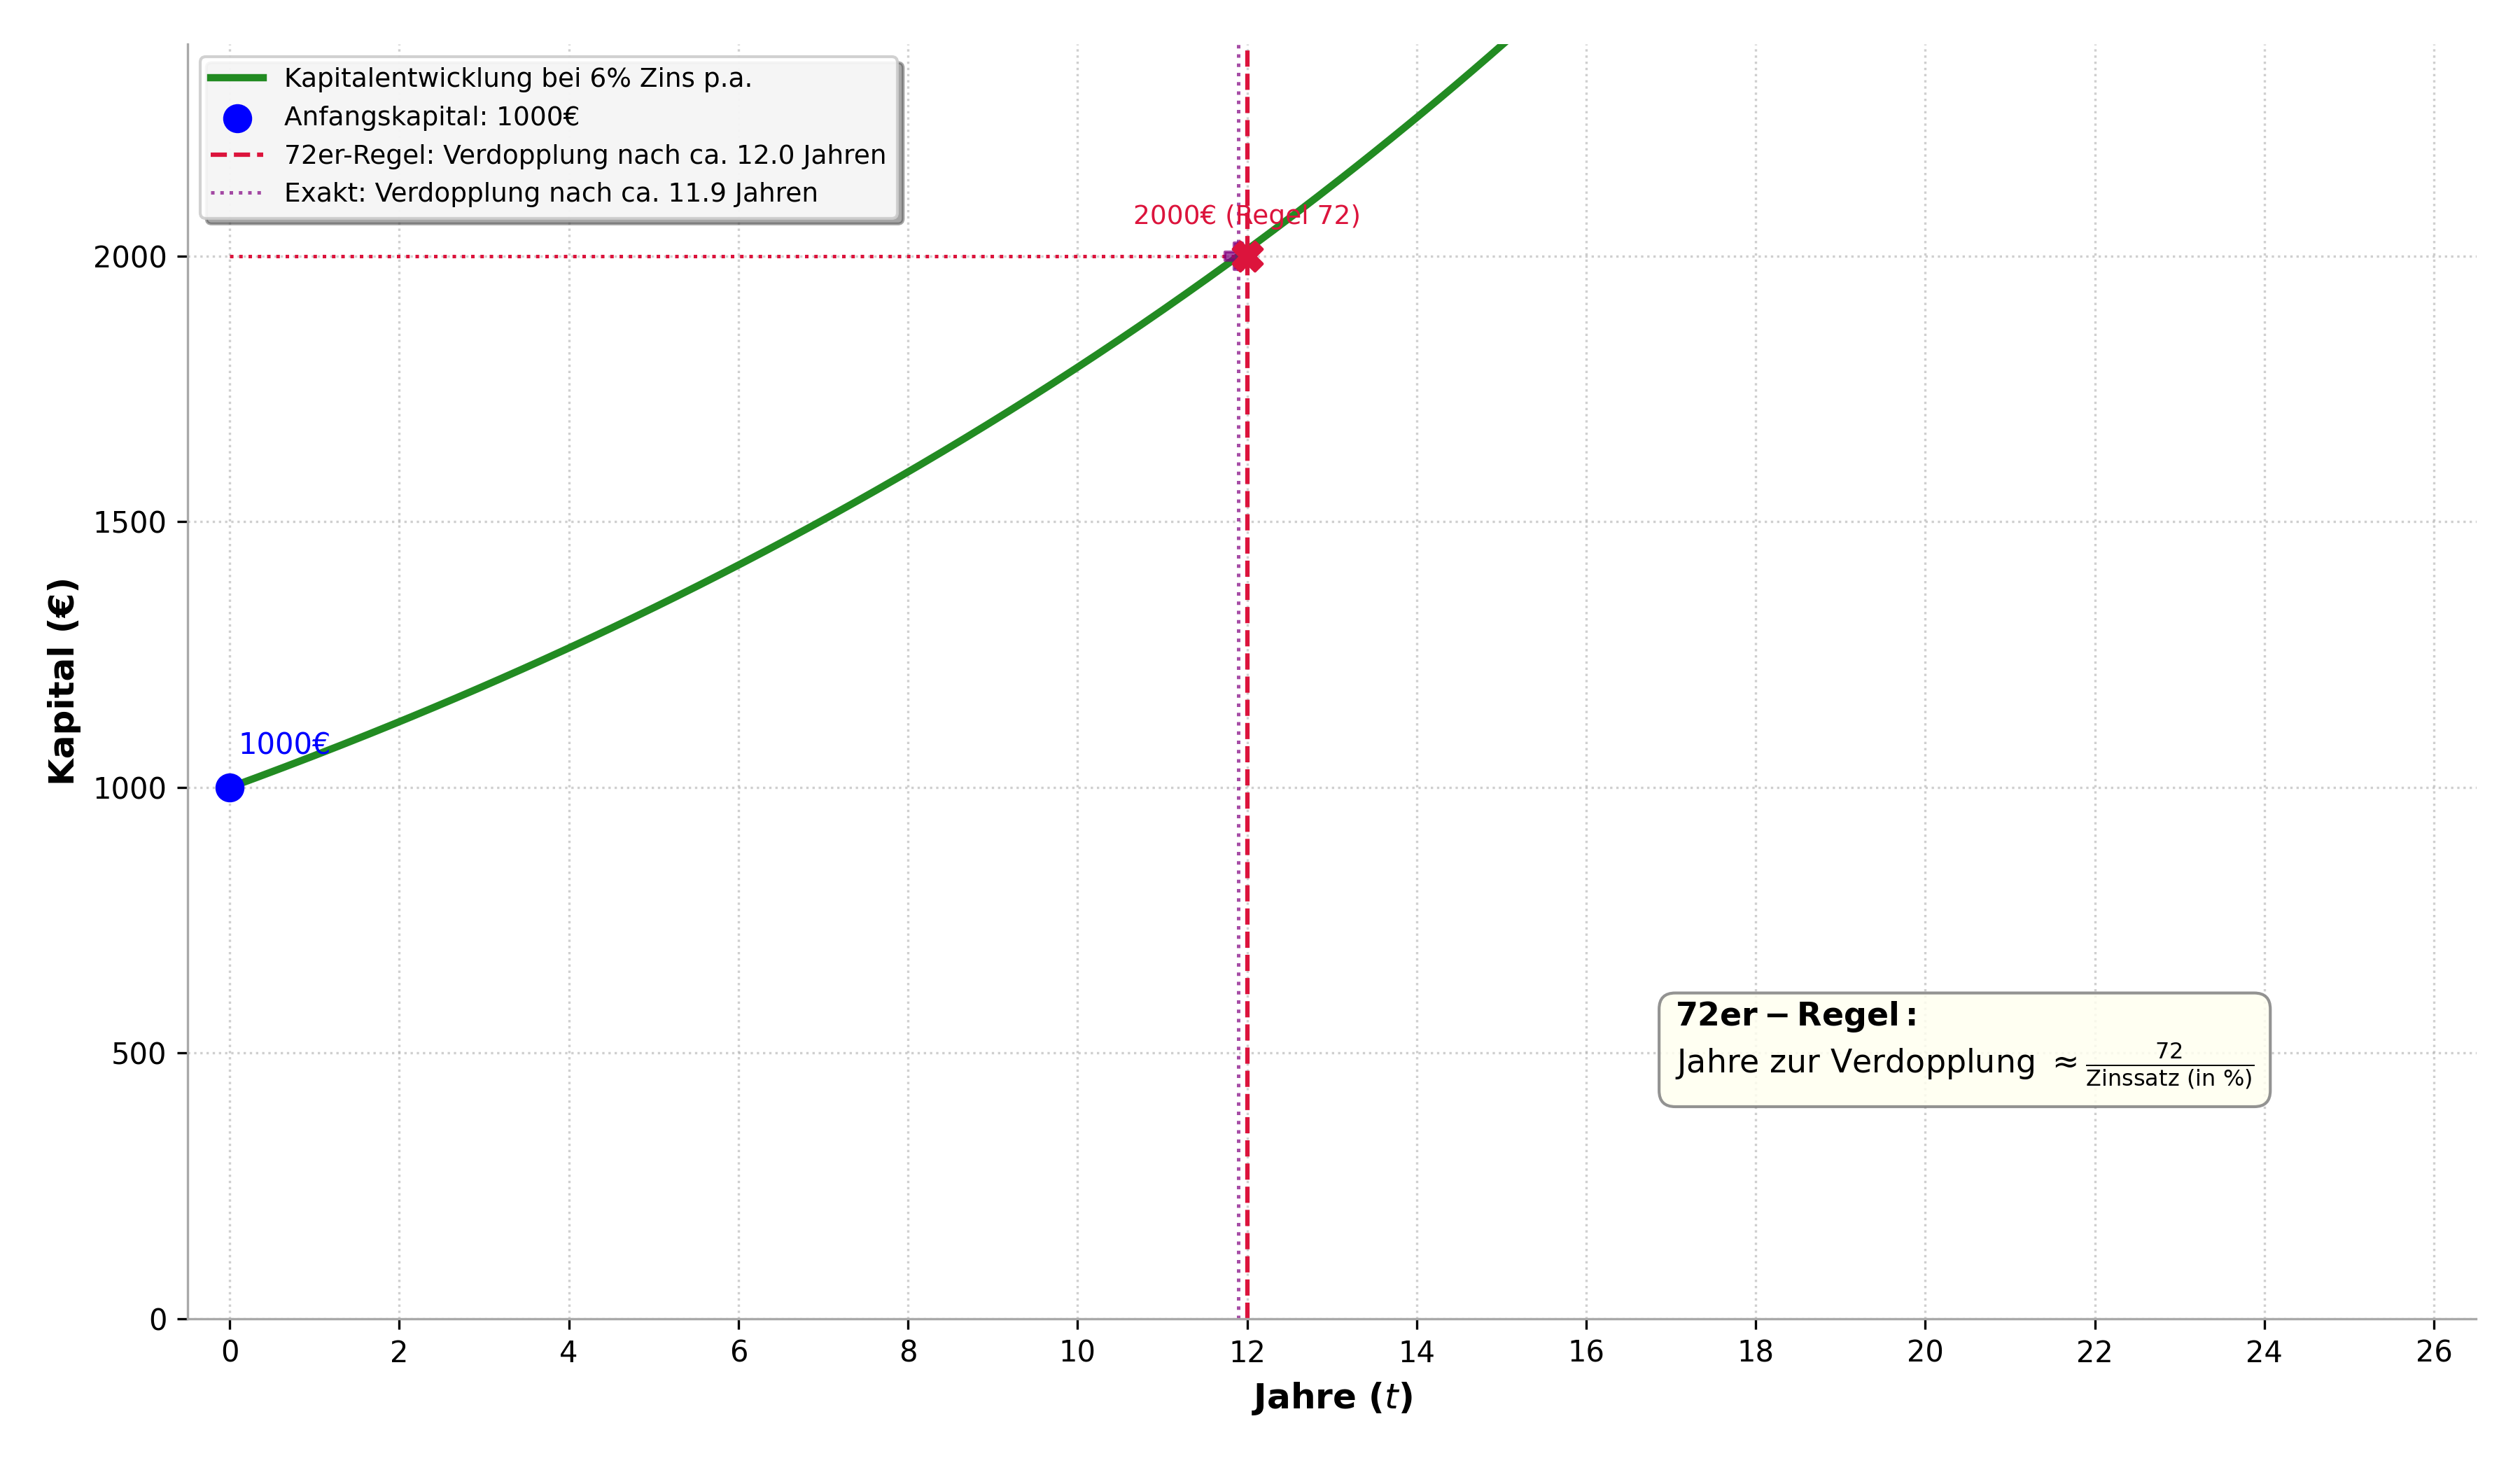
\includegraphics[width=0.5\textwidth]{grafiken/Regel_72_Zins.png}
    % Beschreibung für die Grafik 'Regel_72_Zins.png':
    % Die Grafik könnte ein Sparschwein zeigen, aus dem symbolisch Geld wächst
    % und sich verdoppelt. Daneben die Formel 'ca. 72 / Zinssatz (in %) = Jahre zur Verdopplung'.
    % Oder ein einfacher Graph exponentiellen Wachstums mit einer Markierung, 
    % wo sich der Anfangswert verdoppelt hat.
    \captionof{figure}{Die 72er-Regel: Eine Faustformel zur Verdopplungszeit.}
    \label{fig:regel_72_funfact}
\end{center}
\end{funfactbox}

\subsection{Die natürliche Exponentialfunktion $f(x) = e^x$ und die Eulersche Zahl $e$}
\label{subsec:natuerliche_exp_funktion}

Unter allen Exponentialfunktionen gibt es eine mit einer ganz besonderen Basis, die in der Mathematik eine herausragende Rolle spielt: die \textbf{natürliche Exponentialfunktion} $f(x) = e^x$. Die Basis dieser Funktion ist die \textbf{Eulersche Zahl $e$}.

\begin{merksatzumgebung}{Die Eulersche Zahl $e$}
Die Eulersche Zahl $e$ ist eine irrationale (nicht als Bruch ganzer Zahlen darstellbare) und transzendente Zahl mit dem ungefähren Wert:
\[ e \approx 2,718281828459... \]
Sie ist eine der wichtigsten Konstanten in der Mathematik, ähnlich wie $\pi$.
Eine Möglichkeit, $e$ zu definieren, ist über den Grenzwert (siehe Infobox im vorherigen Kapitel):
\[ e = \lim_{n \to \infty} \left(1 + \frac{1}{n}\right)^n \]
Diese Definition stammt aus der Zinseszinsrechnung bei kontinuierlicher Verzinsung.
\end{merksatzumgebung}

\begin{infoboxumgebung}{Warum ist $e$ so 'natürlich'?}
Die natürliche Exponentialfunktion $f(x)=e^x$ hat eine einzigartige und bemerkenswerte Eigenschaft, die sie so 'natürlich' und fundamental für die Differentialrechnung macht: \textbf{Sie ist ihre eigene Ableitung!}
\[ (e^x)' = e^x \]
Das bedeutet, die Steigung der Tangente an den Graphen von $f(x)=e^x$ an jeder Stelle $x$ ist genau gleich dem Funktionswert $e^x$ an dieser Stelle. An der Stelle $x=0$ ist $f(0)=e^0=1$, und die Steigung der Tangente ist ebenfalls $f'(0)=e^0=1$.
Diese Eigenschaft macht das Rechnen mit $e^x$ besonders elegant.
\end{infoboxumgebung}

\subsubsection{Graph und Eigenschaften von $f(x)=e^x$}

\begin{merksatzumgebung}{Eigenschaften der natürlichen Exponentialfunktion $f(x)=e^x$}
\begin{itemize}
    \item \textbf{Definitionsbereich:} $D_f = \mathbb{R}$ (man kann jede reelle Zahl für $x$ einsetzen).
    \item \textbf{Wertebereich:} $W_f = \mathbb{R}^+ = (0, \infty)$ (die Funktionswerte sind immer positiv und werden niemals Null oder negativ).
    \item \textbf{Nullstellen:} Die Funktion $f(x)=e^x$ hat \textbf{keine Nullstellen}, da $e^x > 0$ für alle $x \in \mathbb{R}$. Der Graph schneidet die x-Achse nie.
    \item \textbf{Schnittpunkt mit der y-Achse:} $f(0) = e^0 = 1$. Der Punkt ist $P_y(0|1)$.
    \item \textbf{Monotonie:} Da die Ableitung $f'(x)=e^x$ immer positiv ist ($e^x > 0$ für alle $x$), ist die Funktion $f(x)=e^x$ \textbf{streng monoton steigend} für alle $x \in \mathbb{R}$.
    \item \textbf{Krümmung:} Die zweite Ableitung ist $f''(x)=(e^x)'=e^x$. Da $f''(x)=e^x$ immer positiv ist, ist der Graph von $f(x)=e^x$ für alle $x \in \mathbb{R}$ \textbf{linksgekrümmt} (konvex).
    \item \textbf{Grenzwerte (Verhalten im Unendlichen):}
        \begin{itemize}
            \item $\lim_{x \to \infty} e^x = +\infty$ (für große positive $x$ werden die Werte beliebig groß).
            \item $\lim_{x \to -\infty} e^x = 0$ (für große negative $x$ nähern sich die Werte der Null an; die x-Achse ist eine \textbf{waagerechte Asymptote} für $x \to -\infty$).
        \end{itemize}
\end{itemize}
\end{merksatzumgebung}

\begin{center}
    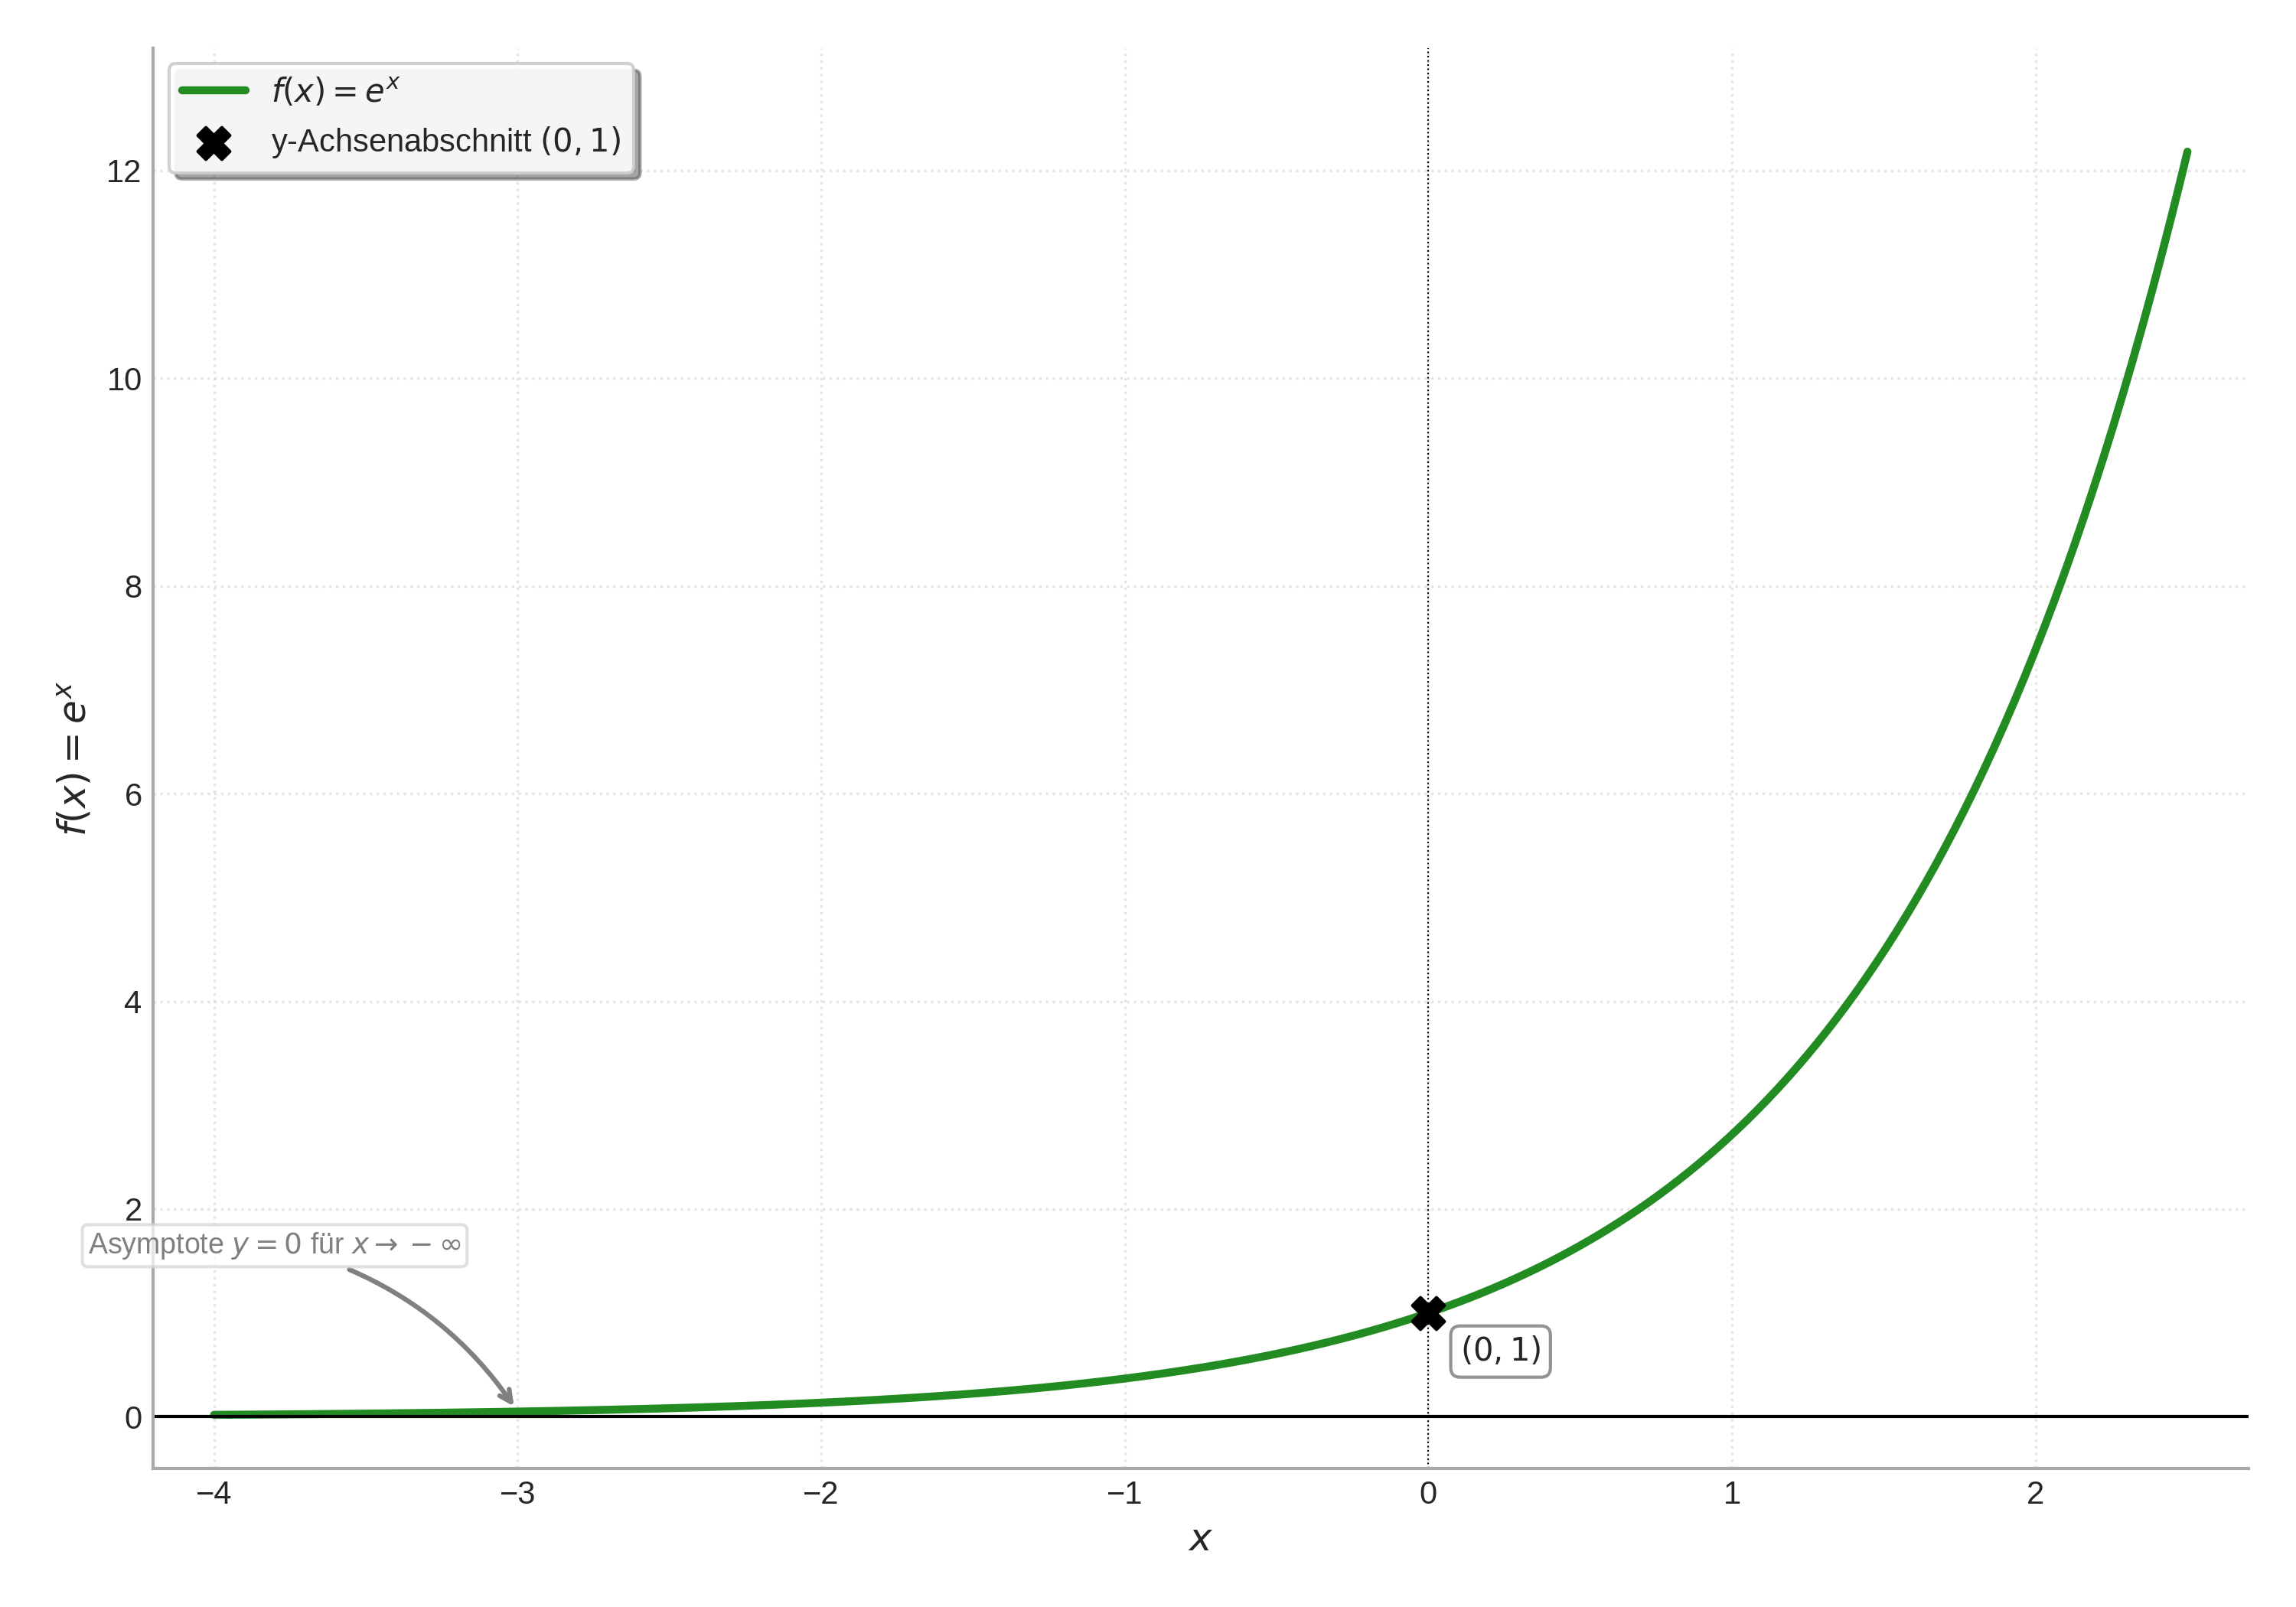
\includegraphics[width=0.8\textwidth]{grafiken/Exponentialfunktion_ex.png}
    \captionof{figure}{Graph der natürlichen Exponentialfunktion $f(x)=e^x$}
    \label{fig:exp_funktion_ex}
\end{center}

\subsubsection{Ableitung und Stammfunktion von $e^x$}

Wie bereits erwähnt, ist das Ableiten von $e^x$ besonders einfach.

\begin{merksatzumgebung}{Ableitung und Stammfunktion von $f(x)=e^x$}
\begin{itemize}
    \item \textbf{Ableitung:} Die Ableitung der natürlichen Exponentialfunktion $f(x)=e^x$ ist die Funktion selbst:
    \[ (e^x)' = e^x \]
    \item \textbf{Stammfunktion (unbestimmtes Integral):} Da die Ableitung von $e^x$ wieder $e^x$ ist, ist $e^x$ auch eine Stammfunktion von sich selbst. Die Menge aller Stammfunktionen ist:
    \[ \int e^x \,dx = e^x + C \]
    wobei $C$ die Integrationskonstante ist.
\end{itemize}
\end{merksatzumgebung}

\begin{beispielumgebung}{Ableiten und Integrieren von $e^x$}
\begin{enumerate}
    \item Leite $f(x) = 5e^x - 3x^2$ ab.
        $f'(x) = (5e^x)' - (3x^2)' = 5(e^x)' - 3(2x) = 5e^x - 6x$.
    \item Bestimme das unbestimmte Integral von $g(x) = 2e^x + 4x$.
        $\int (2e^x + 4x) \,dx = \int 2e^x \,dx + \int 4x \,dx$
        $= 2 \int e^x \,dx + 4 \int x^1 \,dx$
        $= 2e^x + 4 \cdot \frac{1}{2}x^2 + C = 2e^x + 2x^2 + C$.
\end{enumerate}
\end{beispielumgebung}

\begin{aufgabenumgebung}{Erste Übungen mit $e^x$}
\begin{enumerate}
    \item Bilde die erste und zweite Ableitung der folgenden Funktionen:
        \begin{itemize}
            \item $f_1(x) = 3e^x - x^3 + 2x - 7$
            \item $f_2(x) = -0.5e^x + \frac{1}{x}$ (Tipp: $\frac{1}{x} = x^{-1}$)
        \end{itemize}
    \item Bestimme die Menge aller Stammfunktionen:
        \begin{itemize}
            \item $g_1(x) = 4e^x + 6x^2 - 1$
            \item $g_2(x) = \frac{e^x}{2} - \sqrt{x}$ (Tipp: $\frac{e^x}{2} = \frac{1}{2}e^x$)
        \end{itemize}
    \item Berechne das bestimmte Integral $\int_0^1 e^x \,dx$. Was stellt dieser Wert geometrisch dar?
\end{enumerate}
\end{aufgabenumgebung}

\subsection{Allgemeinere Exponentialfunktionen und ihre Transformationen}
\label{subsec:allgemeine_exp_funktionen}

Die natürliche Exponentialfunktion $f(x)=e^x$ ist die Basis, aber oft begegnen uns Exponentialfunktionen in allgemeinerer Form, z.B. $f(x) = a \cdot e^{kx} + d$ oder $f(x) = a \cdot b^x$. Diese entstehen durch Transformationen (Streckung, Stauchung, Spiegelung, Verschiebung) der Grundfunktion $e^x$ oder einer anderen Basis $b$.

\subsubsection{Transformationen der natürlichen Exponentialfunktion: $f(x) = a \cdot e^{k(x-c)} + d$}

Ähnlich wie bei Polynomfunktionen können wir die Parameter interpretieren:
\begin{itemize}
    \item $a$: Streckung/Stauchung in y-Richtung. Wenn $a<0$, zusätzlich Spiegelung an der x-Achse.
    \item $k$: Streckung/Stauchung in x-Richtung. Wenn $k<0$, zusätzlich Spiegelung an der y-Achse. Beeinflusst die 'Schnelligkeit' des Wachstums/Zerfalls.
    \item $c$: Verschiebung in x-Richtung (um $c$ nach rechts, wenn $x-c$; um $c$ nach links, wenn $x+c$).
    \item $d$: Verschiebung in y-Richtung. Die Gerade $y=d$ wird zur neuen \textbf{waagerechten Asymptote}.
\end{itemize}

\textbf{Ableitung von $f(x) = e^{kx}$ (mit Kettenregel):}
Hier ist die äußere Funktion $g(u)=e^u$ mit $g'(u)=e^u$.
Die innere Funktion ist $h(x)=kx$ mit $h'(x)=k$.
Nach der Kettenregel: $(e^{kx})' = g'(h(x)) \cdot h'(x) = e^{kx} \cdot k = k e^{kx}$.

\begin{merksatzumgebung}{Ableitung und Stammfunktion von $e^{kx}$}
\begin{itemize}
    \item \textbf{Ableitung:} $(e^{kx})' = k \cdot e^{kx}$ (Kettenregel: 'äußere Ableitung $e^{kx}$ mal innere Ableitung $k$')
    \item \textbf{Stammfunktion:} $\int e^{kx} \,dx = \frac{1}{k} e^{kx} + C$ (für $k \neq 0$)
\end{itemize}
\end{merksatzumgebung}

\begin{beispielumgebung}{Ableiten und Integrieren von $a \cdot e^{kx}$}
\begin{enumerate}
    \item $f(x) = 3e^{2x}$. Hier ist $a=3, k=2$.
        $f'(x) = 3 \cdot (e^{2x})' = 3 \cdot (2e^{2x}) = 6e^{2x}$.
    \item $g(x) = -4e^{-0.5x} + 7$.
        $g'(x) = -4 \cdot (e^{-0.5x})' + (7)' = -4 \cdot (-0.5 e^{-0.5x}) + 0 = 2e^{-0.5x}$.
    \item $\int 5e^{3x} \,dx = 5 \int e^{3x} \,dx = 5 \cdot \frac{1}{3}e^{3x} + C = \frac{5}{3}e^{3x} + C$.
    \item $\int (e^{-x} + 2) \,dx = \int e^{-1x} \,dx + \int 2 \,dx = \frac{1}{-1}e^{-x} + 2x + C = -e^{-x} + 2x + C$.
\end{enumerate}
\end{beispielumgebung}

\begin{aufgabenumgebung}{Transformationen und Ableitungen/Stammfunktionen}
\begin{enumerate}
    \item Beschreibe, wie der Graph der Funktion $f(x) = 2e^{-0.5(x-1)} + 3$ aus dem Graphen der natürlichen Exponentialfunktion $y=e^x$ hervorgeht. Gib den Definitionsbereich, Wertebereich und die Gleichung der Asymptote an. Skizziere den Graphen.
    \item Bilde die erste Ableitung der folgenden Funktionen:
        \begin{itemize}
            \item $f_1(x) = 7e^{4x}$
            \item $f_2(x) = e^{-x} + 3x$
            \item $f_3(t) = A \cdot e^{-kt}$ ($A, k$ sind positive Konstanten; oft Modell für Zerfall)
        \end{itemize}
    \item Bestimme die Menge aller Stammfunktionen:
        \begin{itemize}
            \item $g_1(x) = 10e^{0.2x}$
            \item $g_2(x) = e^{-3x} - e^{2x}$
        \end{itemize}
\end{enumerate}
\end{aufgabenumgebung}

% Hier geht es dann weiter mit allgemeinen Basen b^x, Produkt/Quotient/Kette mit e-Funktionen, Kurvendiskussionen und Anwendungen.


% Vorheriger Inhalt des Kapitels bis zur aufgabenumgebung 'Transformationen und Ableitungen/Stammfunktionen'
% ... (siehe vorherige Canvas-Version) ...

\subsubsection{Die allgemeine Exponentialfunktion $f(x) = b^x$ und ihre Beziehung zu $e^x$}
\label{subsubsec:allgemeine_basis_b}

Neben der natürlichen Exponentialfunktion $f(x)=e^x$ gibt es natürlich auch Exponentialfunktionen zu jeder beliebigen positiven Basis $b$ (wobei $b \neq 1$), wie zum Beispiel $f(x)=2^x$, $f(x)=10^x$ oder $f(x)=(0.5)^x$.

\begin{merksatzumgebung}{Die allgemeine Exponentialfunktion $f(x)=b^x$}
Eine Funktion der Form
\[ f(x) = b^x \]
mit einer festen Basis $b > 0$ und $b \neq 1$ heißt allgemeine Exponentialfunktion zur Basis $b$.
\begin{itemize}
    \item Wenn $b > 1$: Die Funktion ist streng monoton steigend (Wachstum).
    \item Wenn $0 < b < 1$: Die Funktion ist streng monoton fallend (Zerfall).
\end{itemize}
Alle diese Funktionen gehen durch den Punkt $(0|1)$, denn $b^0=1$.
Ihre waagerechte Asymptote ist die x-Achse ($y=0$) für $x \to -\infty$ (wenn $b>1$) oder für $x \to \infty$ (wenn $0<b<1$).
\end{merksatzumgebung}

\begin{infoboxumgebung}{Warum reicht es oft, $e^x$ zu betrachten? Der Trick mit dem Logarithmus!}
Jede Exponentialfunktion $f(x)=b^x$ (mit $b>0$) lässt sich mit Hilfe des natürlichen Logarithmus ($\ln$) und der $e$-Funktion umschreiben. Es gilt nämlich:
\[ b = e^{\ln(b)} \]
(Da $e^x$ und $\ln(x)$ Umkehrfunktionen voneinander sind, heben sie sich sozusagen gegenseitig auf).
Damit können wir schreiben:
\[ b^x = (e^{\ln(b)})^x \]
Nach den Potenzgesetzen ($(a^m)^n = a^{m \cdot n}$) gilt:
\[ b^x = e^{\ln(b) \cdot x} = e^{x \ln(b)} \]
Der Term $\ln(b)$ ist dabei einfach eine Konstante für eine feste Basis $b$. Wenn wir also $k = \ln(b)$ setzen, haben wir die Form $e^{kx}$, die wir schon kennen!
Das bedeutet: \textbf{Jede Exponentialfunktion $b^x$ kann als natürliche Exponentialfunktion $e^{kx}$ mit $k=\ln(b)$ dargestellt werden.}
Deshalb ist die $e$-Funktion so fundamental: Verstehen wir sie und ihre Transformationen, verstehen wir im Grunde alle Exponentialfunktionen.

\textbf{Beispiele für die Umrechnung:}
\begin{itemize}
    \item $2^x = e^{\ln(2) \cdot x} \approx e^{0.693x}$
    \item $10^x = e^{\ln(10) \cdot x} \approx e^{2.303x}$
    \item $(0.5)^x = e^{\ln(0.5) \cdot x} \approx e^{-0.693x}$ (Hier ist $\ln(0.5) = \ln(1/2) = \ln(1)-\ln(2) = 0-\ln(2) = -\ln(2) < 0$, was zum erwarteten Zerfall führt).
\end{itemize}
\end{infoboxumgebung}

\textbf{Ableitung von $f(x) = b^x$:}
Mit dem Trick $b^x = e^{x \ln(b)}$ und der Kettenregel können wir $b^x$ leicht ableiten:
Sei $f(x) = b^x = e^{x \ln(b)}$.
Die äußere Funktion ist $g(u)=e^u \implies g'(u)=e^u$.
Die innere Funktion ist $h(x)=x \ln(b) \implies h'(x)=\ln(b)$ (da $\ln(b)$ eine Konstante ist und die Ableitung von $kx$ gleich $k$ ist).
Also nach der Kettenregel:
$(b^x)' = (e^{x \ln(b)})' = e^{x \ln(b)} \cdot \ln(b) = b^x \cdot \ln(b)$.

\begin{merksatzumgebung}{Ableitung und Stammfunktion von $f(x)=b^x$}
\begin{itemize}
    \item \textbf{Ableitung:} Die Ableitung der allgemeinen Exponentialfunktion $f(x)=b^x$ ist:
    \[ (b^x)' = b^x \cdot \ln(b) \]
    (Beachte: Für $b=e$ ist $\ln(e)=1$, also $(e^x)' = e^x \cdot 1 = e^x$, was wir schon wussten!)
    \item \textbf{Stammfunktion:} Die Menge aller Stammfunktionen von $f(x)=b^x$ ist:
    \[ \int b^x \,dx = \frac{1}{\ln(b)} b^x + C \quad (\text{für } b>0, b\neq 1) \]
    (Probe: $(\frac{1}{\ln(b)} b^x)' = \frac{1}{\ln(b)} (b^x \cdot \ln(b)) = b^x$. Passt!)
\end{itemize}
\end{merksatzumgebung}

\begin{beispielumgebung}{Ableiten und Integrieren von $b^x$}
\begin{enumerate}
    \item $f(x) = 2^x$.
        $f'(x) = 2^x \cdot \ln(2)$.
    \item $g(x) = 5 \cdot 10^x$.
        $g'(x) = 5 \cdot (10^x \cdot \ln(10)) = 5 \ln(10) \cdot 10^x$.
    \item $\int 3^x \,dx = \frac{1}{\ln(3)} 3^x + C$.
\end{enumerate}
\end{beispielumgebung}

\begin{aufgabenumgebung}{Umgang mit allgemeinen Exponentialfunktionen}
\begin{enumerate}
    \item Schreibe die folgenden Funktionen mit der Basis $e$ (d.h. in der Form $a \cdot e^{kx}$):
        \begin{itemize}
            \item $f_1(x) = 3^x$
            \item $f_2(x) = 10 \cdot (0.8)^x$
        \end{itemize}
    \item Bilde die erste Ableitung der folgenden Funktionen:
        \begin{itemize}
            \item $g_1(x) = 4^x + x^4$
            \item $g_2(x) = 7 \cdot (1.5)^x - e^x$
            \item $g_3(t) = P_0 \cdot a^t$ ($P_0$ und $a$ sind positive Konstanten. Dies ist ein typisches Modell für exponentielles Wachstum oder Zerfall, je nachdem ob $a>1$ oder $0<a<1$.)
        \end{itemize}
    \item Bestimme die Menge aller Stammfunktionen:
        \begin{itemize}
            \item $h_1(x) = 5^x$
            \item $h_2(x) = 3 \cdot (0.2)^x + e^{2x}$
        \end{itemize}
    \item \textbf{Vergleich $2^x$ und $e^x$:}
        \begin{itemize}
            \item Skizziere die Graphen von $f(x)=2^x$ und $g(x)=e^x$ in ein gemeinsames Koordinatensystem (z.B. für $x \in [-2, 3]$). Nutze dazu eine Wertetabelle.
            \item Vergleiche die Steigungen der beiden Funktionen an der Stelle $x=0$. Welche Funktion wächst dort schneller?
            \item Berechne $(2^x)'$ und $(e^x)'$.
        \end{itemize}
\end{enumerate}
\end{aufgabenumgebung}

\begin{fehlerboxumgebung}{Ableiten von $e^{g(x)}$ und $b^x$}
Beim Ableiten von Exponentialfunktionen schleichen sich leicht Fehler ein. Achte besonders auf:
\begin{itemize}
    \item \textbf{Innere Ableitung bei $e^{g(x)}$ vergessen:} Die häufigste Fehlerquelle! Bei Funktionen wie $f(x) = e^{kx}$ oder allgemeiner $f(x) = e^{g(x)}$ musst du immer die Kettenregel anwenden: $(e^{g(x)})' = e^{g(x)} \cdot g'(x)$. Die Ableitung des Exponenten (innere Ableitung $g'(x)$) darf nicht fehlen!
    \textit{Beispiel Falsch:} $(e^{3x})' = e^{3x}$. \textit{Richtig:} $(e^{3x})' = e^{3x} \cdot 3 = 3e^{3x}$.
    \item \textbf{Faktor $\ln(b)$ bei $(b^x)'$ vergessen:} Die Ableitung von $f(x)=b^x$ ist $f'(x) = b^x \cdot \ln(b)$. Der Faktor $\ln(b)$ ist entscheidend (außer für $b=e$, da $\ln(e)=1$).
    \textit{Beispiel Falsch:} $(2^x)' = 2^x$. \textit{Richtig:} $(2^x)' = 2^x \cdot \ln(2)$.
    \item \textbf{Potenzregel falsch auf Basis $e$ oder $b$ angewendet:} Die Regel $(x^n)' = nx^{n-1}$ gilt, wenn die \textit{Basis} die Variable ist und der \textit{Exponent} eine Konstante. Bei $e^x$ oder $b^x$ ist die Basis eine Konstante und der Exponent die Variable.
    \textit{Beispiel Falsch:} $(e^x)' = xe^{x-1}$. \textit{Richtig:} $(e^x)' = e^x$.
\end{itemize}
Präge dir diese Unterschiede gut ein, um Fehler zu vermeiden!
\end{fehlerboxumgebung}

\begin{tippumgebung}{Taschenrechner für $\ln(b)$}
Den Wert von $\ln(b)$ (natürlicher Logarithmus von $b$) findest du auf deinem Taschenrechner (oft als 'ln'-Taste). Für viele theoretische Überlegungen und Ableitungen lässt man $\ln(b)$ aber einfach als exakten Ausdruck stehen.
\end{tippumgebung}

% Vorheriger Inhalt des Kapitels bis zur Tippumgebung 'Taschenrechner für ln(b)'
% ... (siehe vorherige Canvas-Version) ...

Die Fähigkeit, zwischen $b^x$ und $e^{kx}$ wechseln zu können, ist sehr nützlich, da viele Formeln und Regeln in der Analysis primär für die Basis $e$ formuliert sind.

\subsubsection{Anwendung der Ableitungsregeln auf Funktionen mit $e^x$}
\label{subsubsec:ableitungsregeln_ex}

Jetzt, da wir die Grundfunktionen $e^x$ und $e^{kx}$ sowie deren Ableitungen und Stammfunktionen kennen, wollen wir sehen, wie wir Funktionen ableiten, bei denen diese mit Polynomen durch Produkt, Quotient oder Verkettung verbunden sind. Hier kommen unsere bekannten Ableitungsregeln voll zum Einsatz!

\textbf{Produktregel mit $e^x$:}
Erinnerung: $(u \cdot v)' = u'v + uv'$.

\begin{beispielumgebung}{Produktregel mit $e^x$}
Leite $f(x) = x^2 \cdot e^x$ ab.
\begin{itemize}
    \item $u(x) = x^2 \implies u'(x) = 2x$
    \item $v(x) = e^x \implies v'(x) = e^x$
\end{itemize}
$f'(x) = (2x) \cdot e^x + x^2 \cdot e^x$
Hier kann man $e^x$ ausklammern:
$f'(x) = e^x (2x + x^2) = e^x (x^2 + 2x)$.
\end{beispielumgebung}

\begin{aufgabenumgebung}{Produktregel mit $e^x$ üben}
Bilde die erste Ableitung der folgenden Funktionen und vereinfache so weit wie möglich:
\begin{enumerate}
    \item $f_1(x) = (3x-1)e^x$
    \item $f_2(x) = (x^2+2x-5)e^x$
    \item $f_3(t) = t \cdot e^{2t}$ (Hier ist die Kettenregel für $e^{2t}$ zusätzlich nötig!)
\end{enumerate}
\end{aufgabenumgebung}

\textbf{Quotientenregel mit $e^x$:}
Erinnerung: $(\frac{u}{v})' = \frac{u'v - uv'}{v^2}$.

\begin{beispielumgebung}{Quotientenregel mit $e^x$}
Leite $f(x) = \frac{e^x}{x^2+1}$ ab. (Definitionsbereich $D_f = \mathbb{R}$)
\begin{itemize}
    \item $u(x) = e^x \implies u'(x) = e^x$
    \item $v(x) = x^2+1 \implies v'(x) = 2x$
\end{itemize}
$f'(x) = \frac{e^x \cdot (x^2+1) - e^x \cdot 2x}{(x^2+1)^2}$
Auch hier kann man $e^x$ im Zähler ausklammern:
$f'(x) = \frac{e^x (x^2+1 - 2x)}{(x^2+1)^2} = \frac{e^x (x^2-2x+1)}{(x^2+1)^2} = \frac{e^x (x-1)^2}{(x^2+1)^2}$.
\end{beispielumgebung}

\begin{aufgabenumgebung}{Quotientenregel mit $e^x$ üben}
Bilde die erste Ableitung der folgenden Funktionen und vereinfache so weit wie möglich. Gib auch den Definitionsbereich an.
\begin{enumerate}
    \item $f_1(x) = \frac{x+2}{e^x}$
    \item $f_2(x) = \frac{e^{3x}}{2x-1}$ (Kettenregel für $e^{3x}$ nötig!)
\end{enumerate}
\end{aufgabenumgebung}

\textbf{Kettenregel mit $e^x$ (Vertiefung):}
Erinnerung: $(g(h(x)))' = g'(h(x)) \cdot h'(x)$.
Die Exponentialfunktion tritt sehr oft als äußere Funktion auf, wobei der Exponent die innere Funktion ist.

\begin{beispielumgebung}{Kettenregel mit $e^x$ vertieft}
Leite $f(x) = e^{x^2-3x}$ ab.
\begin{itemize}
    \item Äußere Funktion: $g(u) = e^u \implies g'(u) = e^u$.
    \item Innere Funktion: $h(x) = x^2-3x \implies h'(x) = 2x-3$.
\end{itemize}
$f'(x) = g'(h(x)) \cdot h'(x) = e^{x^2-3x} \cdot (2x-3) = (2x-3)e^{x^2-3x}$.
\end{beispielumgebung}

\begin{aufgabenumgebung}{Kettenregel mit $e^x$ weiter üben}
Bilde die erste Ableitung:
\begin{enumerate}
    \item $f_1(x) = e^{-x^2}$
    \item $f_2(x) = 5e^{2x^3-4x+1}$
    \item $f_3(x) = (e^x+1)^3$ (Hier ist $e^x+1$ die innere Funktion und $(\dots)^3$ die äußere.)
\end{enumerate}
\end{aufgabenumgebung}



\begin{aufgabenumgebung}{Kombinierte Anwendung: Produkt- und Kettenregel bei e-Funktionen}
Bilde die erste Ableitung der folgenden Funktionen. Vereinfache das Ergebnis so weit wie möglich, indem du z.B. gemeinsame Faktoren (insbesondere den $e$-Term) ausklammerst.
\begin{enumerate}
    \item $f(x) = (2x^2 - 3x + 1) \cdot e^{x^2 - 4}$
        \begin{tippumgebung}{Struktur erkennen}
        Diese Funktion ist ein Produkt $u(x) \cdot v(x)$. Für die Ableitung des Faktors $v(x)=e^{x^2-4}$ benötigst du die Kettenregel.
        \end{tippumgebung}
    \item $g(x) = (x+1)^2 \cdot e^{-2x}$
        \begin{tippumgebung}{Zweimal Kettenregel?}
        Auch dies ist ein Produkt. Ein Faktor ist $(x+1)^2$, dessen Ableitung die Kettenregel (oder Ausmultiplizieren) erfordert. Der andere Faktor $e^{-2x}$ benötigt ebenfalls die Kettenregel.
        \end{tippumgebung}
\end{enumerate}
\end{aufgabenumgebung}


\subsection{Kurvendiskussion von Funktionen mit $e^x$}
\label{subsec:kurvendiskussion_ex}

Jetzt, da wir wissen, wie man Funktionen mit $e^x$ ableitet, können wir auch für sie eine vollständige Kurvendiskussion durchführen. Ein wichtiger Punkt bei der Nullstellensuche ist die Eigenschaft der $e$-Funktion.

\begin{infoboxumgebung}{Nullstellen von Produkten mit $e^x$ – Eine wichtige Erkenntnis}
Wir wissen, dass $e^x > 0$ für alle reellen Zahlen $x$ gilt. Die natürliche Exponentialfunktion hat also \textbf{keine Nullstellen}.
Das hat eine wichtige Konsequenz für Produkte der Form $f(x) = \text{Polynom}(x) \cdot e^x$ oder allgemeiner $f(x) = h(x) \cdot e^{g(x)}$:
Nach dem Satz vom Nullprodukt ist ein Produkt genau dann Null, wenn mindestens einer seiner Faktoren Null ist. Da $e^x$ (oder $e^{g(x)}$) niemals Null werden kann, hängen die Nullstellen von $f(x)$ \textbf{ausschließlich von den Nullstellen des Faktors $\text{Polynom}(x)$ (bzw. $h(x)$) ab}.

Um die Nullstellen von $f(x) = \text{Polynom}(x) \cdot e^x$ zu finden, reicht es also, die Gleichung $\text{Polynom}(x) = 0$ zu lösen.
\end{infoboxumgebung}

\begin{beispielumgebung}[Kurvendiskussion einer e-Funktion mit Polynom]{Untersuchung von $f(x) = (x-1)e^x$}
\begin{enumerate}
    \item \textbf{Definitionsbereich:} $D_f = \mathbb{R}$ (sowohl $x-1$ als auch $e^x$ sind für alle $x$ definiert).
    \item \textbf{Symmetrie:}
        $f(-x) = (-x-1)e^{-x} = -(x+1)e^{-x}$.
        Keine einfache Symmetrie zum Koordinatensystem erkennbar.
    \item \textbf{Verhalten im Unendlichen:}
        \begin{itemize}
            \item Für $x \to \infty$: $(x-1) \to \infty$ und $e^x \to \infty$. Also $\lim_{x \to \infty} f(x) = \infty \cdot \infty = +\infty$.
            \item Für $x \to -\infty$: $(x-1) \to -\infty$. Aber $e^x \to 0$. Hier haben wir einen Konflikt '$-\infty \cdot 0$'. Es ist bekannt, dass die $e$-Funktion 'stärker' gegen Null geht als jedes Polynom gegen Unendlich. Man kann auch schreiben $f(x) = \frac{x-1}{e^{-x}}$. Für $x \to -\infty$ geht der Zähler gegen $-\infty$ und der Nenner $e^{-x}$ gegen $e^{\infty} = \infty$. Auch hier ist es nicht sofort klar.
            Ein wichtiger Grenzwert ist $\lim_{x \to -\infty} x^n e^x = 0$ für jedes $n \in \mathbb{N}$.
            Daher: $\lim_{x \to -\infty} (x-1)e^x = 0$. Die x-Achse ($y=0$) ist eine waagerechte Asymptote für $x \to -\infty$.
        \end{itemize}
    \item \textbf{y-Achsenabschnitt:} $f(0) = (0-1)e^0 = (-1) \cdot 1 = -1$. Also $P_y(0|-1)$.
    \item \textbf{Nullstellen:} $f(x)=0 \implies (x-1)e^x = 0$.
        Da $e^x \neq 0$ für alle $x$, muss $x-1=0$ sein.
        Also $x_N = 1$. Einzige Nullstelle bei $N(1|0)$.
    \item \textbf{Erste Ableitung $f'(x)$:} Mit Produktregel $u(x)=x-1, u'(x)=1, v(x)=e^x, v'(x)=e^x$.
        $f'(x) = 1 \cdot e^x + (x-1) \cdot e^x = e^x (1 + x - 1) = xe^x$.
    \item \textbf{Extremstellen:} $f'(x)=0 \implies xe^x = 0$.
        Da $e^x \neq 0$, muss $x=0$ sein. Potentielle Extremstelle bei $x_E=0$.
    \item \textbf{Zweite Ableitung $f''(x)$:} Mit Produktregel für $f'(x)=xe^x$: $u(x)=x, u'(x)=1, v(x)=e^x, v'(x)=e^x$.
        $f''(x) = 1 \cdot e^x + x \cdot e^x = e^x(1+x) = (x+1)e^x$.
    \item \textbf{Art der Extremstelle bei $x_E=0$ mit $f''$ prüfen:}
        $f''(0) = (0+1)e^0 = 1 \cdot 1 = 1$.
        Da $f'(0)=0$ und $f''(0)=1 > 0 \implies$ Lokaler Tiefpunkt bei $x_E=0$.
        $y_T = f(0) = -1$. Tiefpunkt $T(0|-1)$. (Das ist auch unser y-Achsenabschnitt).
    \item \textbf{Monotonie:} Nullstelle von $f'(x)=xe^x$ ist $x=0$.
        \begin{itemize}
            \item $x < 0$ (z.B. $x=-1$): $f'(-1) = (-1)e^{-1} = -1/e < 0 \implies$ fallend.
            \item $x > 0$ (z.B. $x=1$): $f'(1) = (1)e^{1} = e > 0 \implies$ steigend.
        \end{itemize}
        Fallend für $x \in (-\infty, 0]$, steigend für $x \in [0, \infty)$.
    \item \textbf{Wendepunkte:} $f''(x_W)=0 \implies (x_W+1)e^{x_W} = 0$.
        Da $e^{x_W} \neq 0$, muss $x_W+1=0 \implies x_W = -1$.
        Dritte Ableitung $f'''(x)$: Produktregel für $f''(x)=(x+1)e^x$. $u(x)=x+1, u'(x)=1, v(x)=e^x, v'(x)=e^x$.
        $f'''(x) = 1 \cdot e^x + (x+1)e^x = e^x(1+x+1) = (x+2)e^x$.
        $f'''(-1) = (-1+2)e^{-1} = 1 \cdot e^{-1} = 1/e \neq 0$.
        Also Wendepunkt bei $x_W=-1$.
        $y_W = f(-1) = (-1-1)e^{-1} = -2e^{-1} = -2/e \approx -0.736$.
        Wendepunkt $W(-1|-2/e)$.
    \item \textbf{Krümmungsverhalten:} Nullstelle von $f''(x)=(x+1)e^x$ ist $x=-1$.
        \begin{itemize}
            \item $x < -1$ (z.B. $x=-2$): $f''(-2) = (-2+1)e^{-2} = -e^{-2} < 0 \implies$ rechtsgekrümmt.
            \item $x > -1$ (z.B. $x=0$): $f''(0) = (0+1)e^{0} = 1 > 0 \implies$ linksgekrümmt.
        \end{itemize}
    \item \textbf{Skizze:}
        \begin{center}
            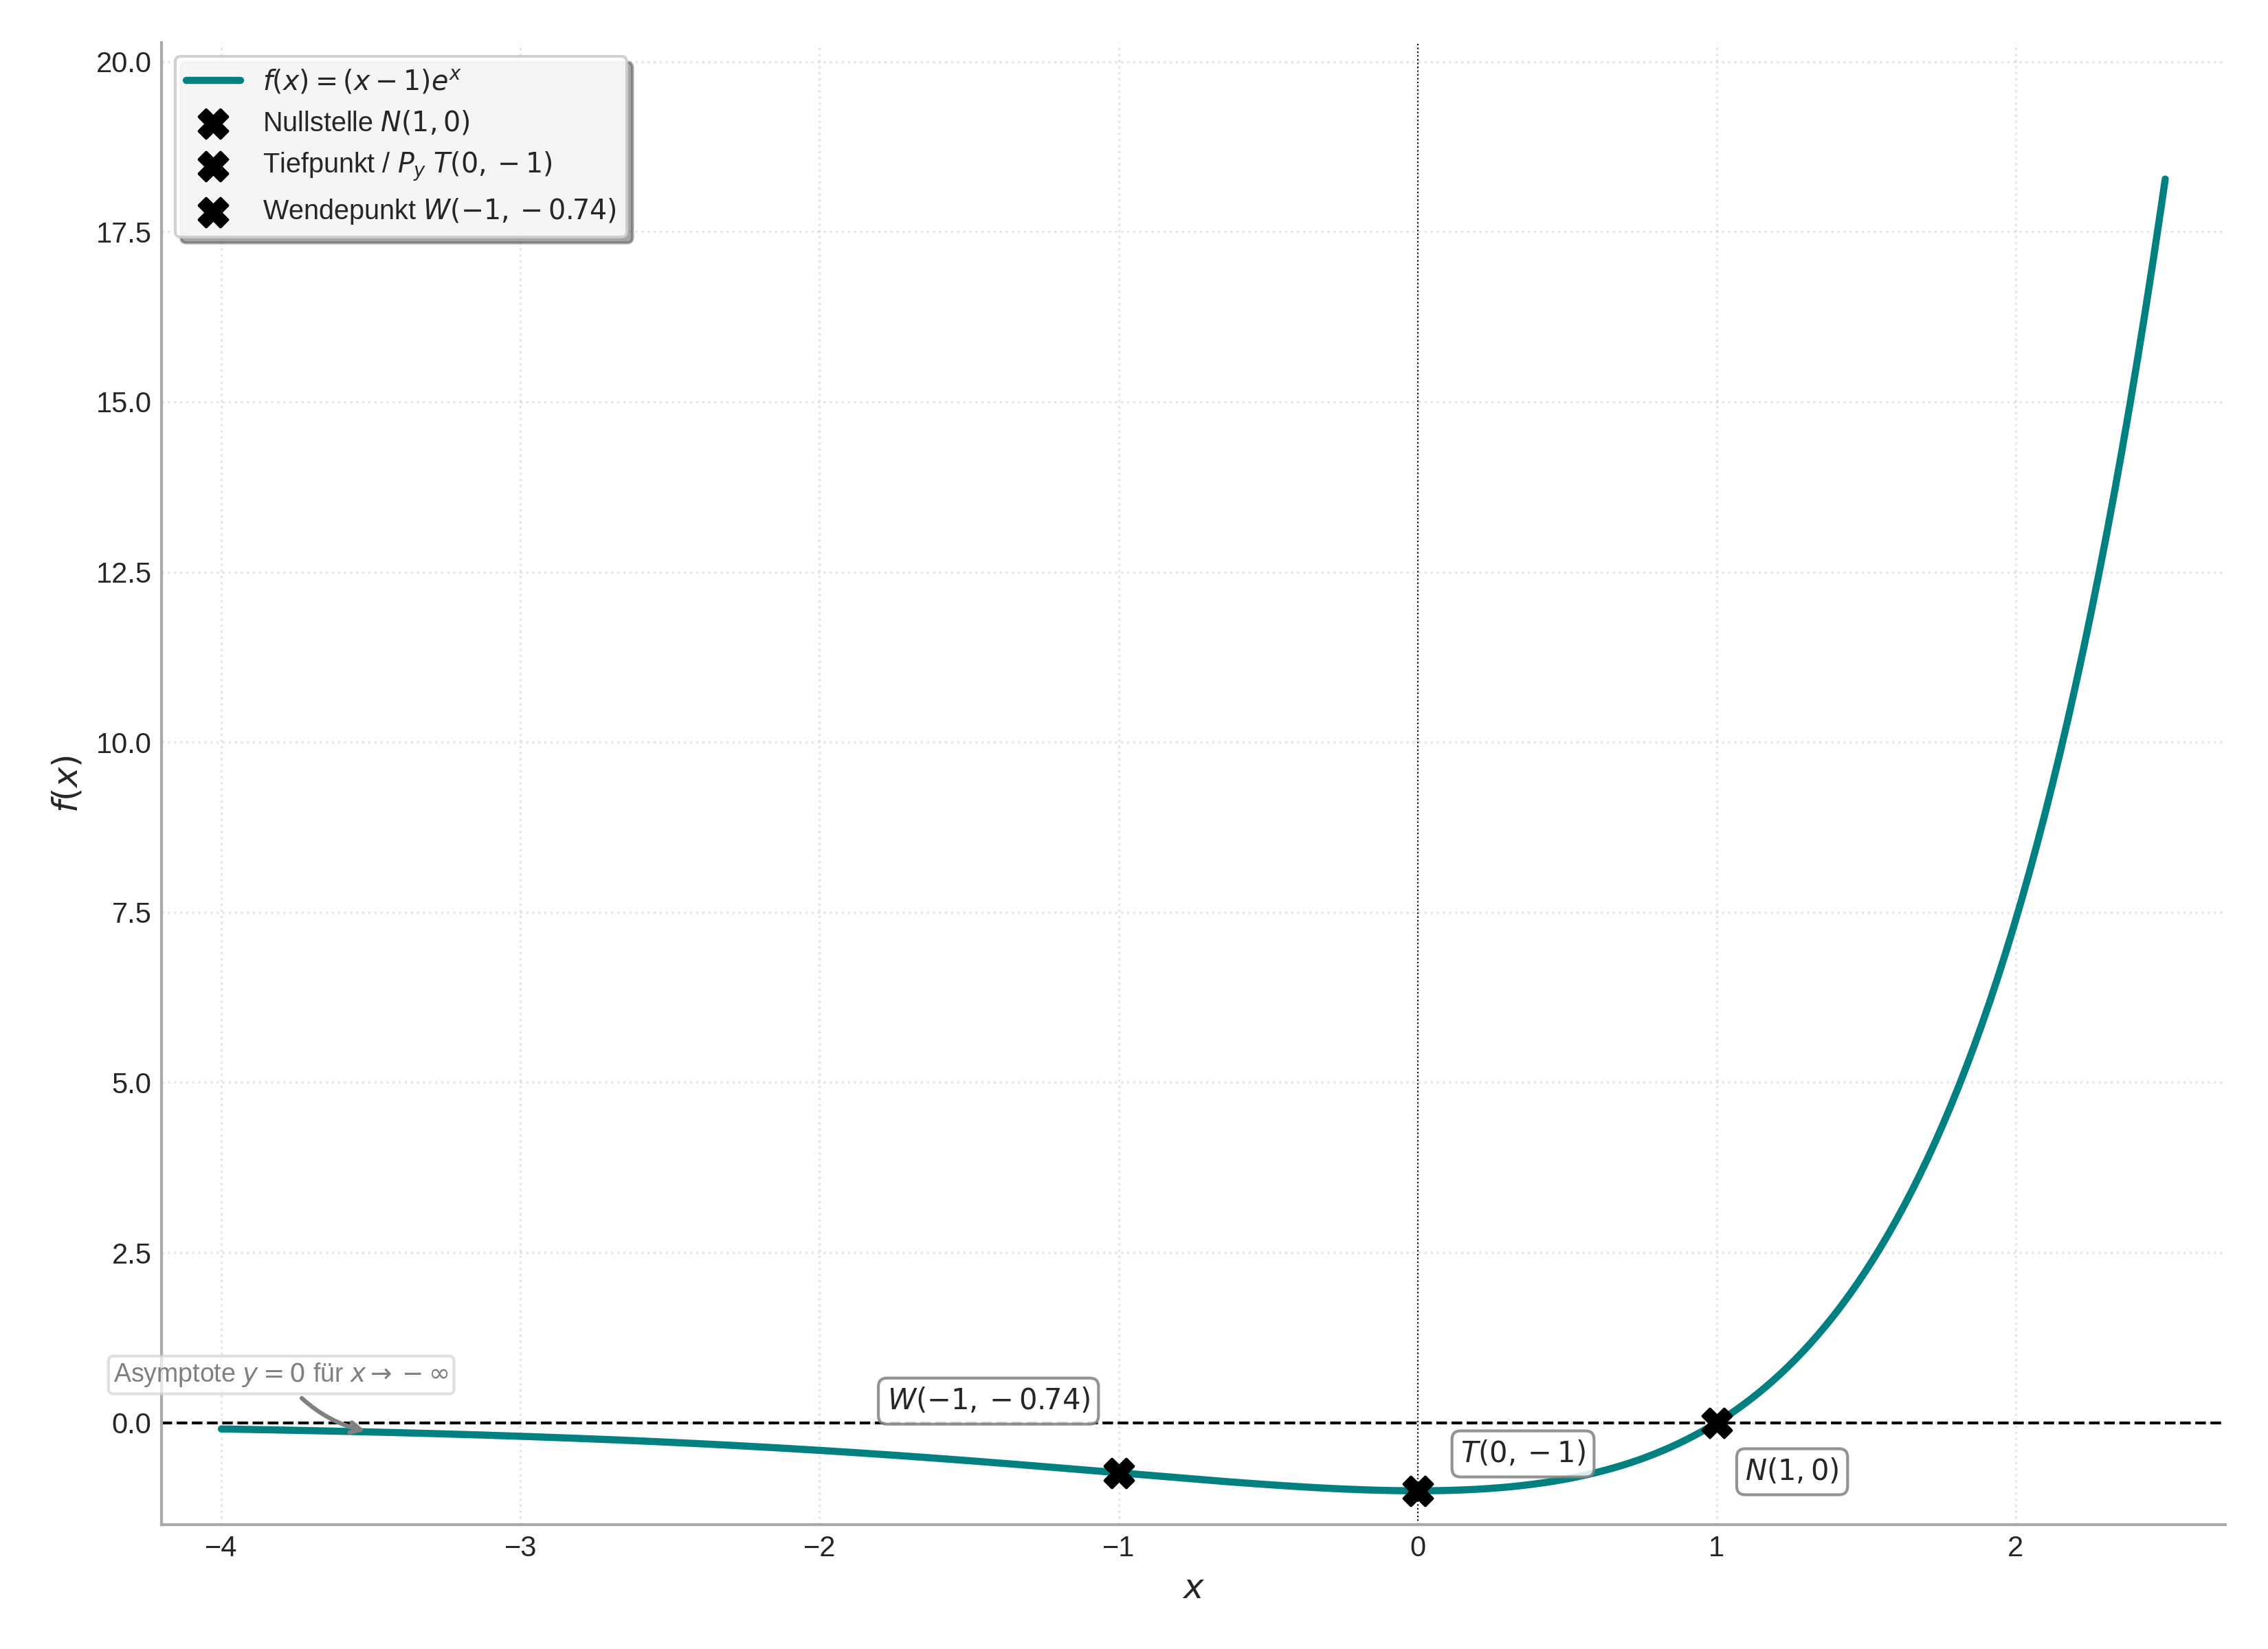
\includegraphics[width=0.9\textwidth]{grafiken/Kurvendiskussion_eFunktion_Polynom.png}
            \captionof{figure}{Graph von $f(x)=(x-1)e^x$}
            \label{fig:kurvendisk_ex_polynom}
        \end{center}
\end{enumerate}
\end{beispielumgebung}


% ... (Nach Beispiel 7.7 und der zugehörigen Abbildung \ref{fig:kurvendisk_ex_polynom}) ...

\begin{infoboxumgebung}{Die Regel von L'Hôpital – Grenzwerte bei '$\frac{0}{0}$' oder '$\frac{\infty}{\infty}$'}
Manchmal stoßen wir bei der Berechnung von Grenzwerten auf unbestimmte Ausdrücke wie '$\frac{0}{0}$' oder '$\frac{\pm\infty}{\pm\infty}$'. Eine direkte Einsetzung des Grenzwertes ist dann nicht möglich. Für solche Fälle gibt es eine elegante Methode, die nach dem französischen Mathematiker Guillaume de L'Hôpital (1661-1704) benannt ist.

\textbf{Die Regel von L'Hôpital:}
Seien $f(x)$ und $g(x)$ zwei differenzierbare Funktionen. Wenn der Grenzwert des Quotienten $\frac{f(x)}{g(x)}$ für $x \to a$ (wobei $a$ eine Zahl, $\infty$ oder $-\infty$ sein kann) einen der folgenden unbestimmten Ausdrücke ergibt:
\begin{itemize}
    \item $\lim_{x \to a} f(x) = 0$ und $\lim_{x \to a} g(x) = 0$ (Fall '$\frac{0}{0}$')
    \item $\lim_{x \to a} f(x) = \pm\infty$ und $\lim_{x \to a} g(x) = \pm\infty$ (Fall '$\frac{\pm\infty}{\pm\infty}$')
\end{itemize}
Dann gilt, vorausgesetzt der Grenzwert auf der rechten Seite existiert (oder ist $\pm\infty$):
\[ \lim_{x \to a} \frac{f(x)}{g(x)} = \lim_{x \to a} \frac{f'(x)}{g'(x)} \]
\textbf{Wichtig:} Man leitet Zähler und Nenner \textbf{getrennt} voneinander ab, nicht mit der Quotientenregel! Die Regel kann bei Bedarf auch mehrfach hintereinander angewendet werden, solange die Voraussetzungen erfüllt sind.

\textbf{Was ist mit dem Fall '$0 \cdot \infty$'?}
Auch diesen unbestimmten Ausdruck kann man oft auf die Form '$\frac{0}{0}$' oder '$\frac{\infty}{\infty}$' bringen, um L'Hôpital anwenden zu können. Zum Beispiel kann man $f(x) \cdot g(x)$ umschreiben zu $\frac{f(x)}{1/g(x)}$ oder $\frac{g(x)}{1/f(x)}$.

\textbf{Beispiele (mit $e^x$ und Polynomen):}
\begin{enumerate}
    \item \textbf{Fall '$\frac{0}{0}$':} $\lim_{x \to 0} \frac{e^x - 1 - x}{x^2}$
        \begin{itemize}
            \item Für $x \to 0$: Zähler $e^0 - 1 - 0 = 1-1-0=0$. Nenner $0^2=0$. (Fall '$\frac{0}{0}$')
            \item Ableitungen: $f(x) = e^x-1-x \implies f'(x) = e^x-1$. $g(x) = x^2 \implies g'(x) = 2x$.
            \item $\lim_{x \to 0} \frac{e^x-1}{2x}$. Für $x \to 0$: Zähler $e^0-1=0$. Nenner $2 \cdot 0=0$. (Wieder '$\frac{0}{0}$')
            \item Erneute Anwendung von L'Hôpital:
            Ableitungen: $(e^x-1)' = e^x$. $(2x)' = 2$.
            \item $\lim_{x \to 0} \frac{e^x}{2} = \frac{e^0}{2} = \frac{1}{2}$.
        \end{itemize}
    \item \textbf{Fall '$\frac{\infty}{\infty}$' und die 'Stärke' von $e^x$:} $\lim_{x \to \infty} \frac{x^2}{e^x}$
        \begin{itemize}
            \item Für $x \to \infty$: Zähler $x^2 \to \infty$. Nenner $e^x \to \infty$. (Fall '$\frac{\infty}{\infty}$')
            \item Ableitungen: $(x^2)' = 2x$. $(e^x)' = e^x$.
            \item $\lim_{x \to \infty} \frac{2x}{e^x}$. Für $x \to \infty$: Zähler $2x \to \infty$. Nenner $e^x \to \infty$. (Wieder '$\frac{\infty}{\infty}$')
            \item Erneute Anwendung von L'Hôpital:
            Ableitungen: $(2x)' = 2$. $(e^x)' = e^x$.
            \item $\lim_{x \to \infty} \frac{2}{e^x}$. Da $e^x \to \infty$, geht der Bruch gegen $0$. Also: $\lim_{x \to \infty} \frac{x^2}{e^x} = 0$.
        \end{itemize}
        \textit{Erklärung zur Dominanz von $e^x$:} Dieses Beispiel zeigt, warum $e^x$ (für $x \to \infty$) 'stärker wächst' als jedes Polynom $x^n$. Bei jeder Anwendung der Regel von L'Hôpital wird der Grad des Polynoms im Zähler um 1 reduziert, bis schließlich eine Konstante übrig bleibt. Die $e^x$-Funktion im Nenner bleibt jedoch bei jeder Ableitung (bis auf eventuelle konstante Faktoren bei $e^{kx}$) im Wesentlichen erhalten und strebt weiterhin gegen $\infty$. Daher wird der Grenzwert des Bruchs letztendlich Null.

    \item \textbf{Fall '$0 \cdot \infty$':} $\lim_{x \to -\infty} x e^x$ (aus Beispiel 7.7)
        \begin{itemize}
            \item Für $x \to -\infty$: $x \to -\infty$ und $e^x \to 0$. (Fall '$-\infty \cdot 0$')
            \item Umformen zu '$\frac{-\infty}{\infty}$': $x e^x = \frac{x}{e^{-x}}$. Für $x \to -\infty$: Zähler $x \to -\infty$. Nenner $e^{-x} \to e^{\infty} \to \infty$.
            \item Ableitungen: $(x)' = 1$. $(e^{-x})' = -e^{-x}$ (Kettenregel).
            \item $\lim_{x \to -\infty} \frac{1}{-e^{-x}}$. Für $x \to -\infty$: Nenner $-e^{-x} \to -e^{\infty} \to -\infty$.
            \item Der Bruch $\frac{1}{-\infty}$ geht gegen $0$. Also: $\lim_{x \to -\infty} x e^x = 0$.
        \end{itemize}
\end{enumerate}
\textbf{Achtung:} Die Regel von L'Hôpital darf nur angewendet werden, wenn tatsächlich einer der unbestimmten Ausdrücke '$\frac{0}{0}$' oder '$\frac{\pm\infty}{\pm\infty}$' vorliegt! Eine falsche Anwendung führt zu falschen Ergebnissen.
\end{infoboxumgebung}


\begin{aufgabenumgebung}{Kurvendiskussionen mit Exponentialfunktionen}
Führe eine vollständige Kurvendiskussion für die folgenden Funktionen durch.
\begin{enumerate}
    \item $f(x) = x e^{-x}$
    \item $g(x) = (x^2-2)e^x$
    \item \textbf{Für Experten:} $h(x) = e^{x^2-2x}$. (Hier wird die Kettenregel komplexer, aber die Struktur der Kurvendiskussion bleibt gleich.)
\end{enumerate}
\end{aufgabenumgebung}

\begin{tippumgebung}{Anwendungsaufgaben mit Exponentialfunktionen}
Exponentialfunktionen sind ideal, um Prozesse zu beschreiben, bei denen die Änderungsrate vom Bestand abhängt.
\begin{itemize}
    \item \textbf{Wachstum:} $N(t) = N_0 \cdot e^{kt}$ mit $k>0$ (z.B. Bakterienkultur, Zinseszins bei stetiger Verzinsung). $N_0$ ist der Anfangsbestand.
    \item \textbf{Zerfall:} $N(t) = N_0 \cdot e^{-kt}$ mit $k>0$ (z.B. radioaktiver Zerfall, Abklingvorgänge). $N_0$ ist der Anfangsbestand. Die Konstante $k$ wird oft als Zerfallskonstante bezeichnet.
    \item \textbf{Logistisches Wachstum (Ausblick):} Für begrenztes Wachstum gibt es komplexere Modelle wie $N(t) = \frac{G}{1+e^{-kG(t-t_0)}}$, die eine Sättigungsgrenze $G$ haben.
\end{itemize}
Bei solchen Aufgaben geht es oft darum, die Parameter ($N_0, k$) aus gegebenen Bedingungen zu bestimmen oder Vorhersagen zu treffen.
\end{tippumgebung}

\begin{aufgabenumgebung}{Anwendung: Radioaktiver Zerfall}
Eine radioaktive Substanz zerfällt so, dass die noch vorhandene Menge $M(t)$ (in Gramm) nach $t$ Jahren durch die Funktion $M(t) = 100 \cdot e^{-0.05t}$ beschrieben wird.
\begin{enumerate}
    \item Wie groß ist die Anfangsmenge der Substanz?
    \item Wie viel Gramm sind nach 10 Jahren noch vorhanden?
    \item Mit welcher Rate zerfällt die Substanz zum Zeitpunkt $t=0$ und zum Zeitpunkt $t=10$ Jahre (in Gramm pro Jahr)? (Tipp: Ableitung $M'(t)$).
    \item \textbf{Halbwertszeit:} Nach welcher Zeit $T_H$ ist nur noch die Hälfte der ursprünglichen Menge vorhanden? (Setze $M(T_H) = \frac{1}{2}M(0)$ und löse nach $T_H$. Hierfür benötigst du den natürlichen Logarithmus $\ln$, die Umkehrfunktion von $e^x$.)
\end{enumerate}
\end{aufgabenumgebung}

% Vorheriger Inhalt des Kapitels bis zur Aufgabe 'Anwendung: Radioaktiver Zerfall'
% ... (siehe vorherige Canvas-Version) ...

\subsubsection{Weitere anspruchsvolle Aufgaben mit Exponentialfunktionen}
\label{subsubsec:exp_anwendungen_vertiefung}

Die folgenden Aufgaben kombinieren die Ableitung von Exponentialfunktionen mit den Konzepten der Kurvendiskussion und Anwendungen. Sie erfordern oft mehrere Ableitungsregeln und ein gutes Verständnis der Zusammenhänge.

\begin{aufgabenumgebung}{Optimierung im biologischen Kontext – Wachstum und Hemmung}
Eine Bakterienpopulation wächst zunächst, wird aber durch einen hemmenden Faktor (z.B. begrenzte Nährstoffe) beeinflusst. Die Anzahl der Bakterien $N$ (in Tausend) nach $t$ Stunden kann modelliert werden durch die Funktion:
\[ N(t) = 5t \cdot e^{-0.1t} \quad (\text{für } t \ge 0) \]
\begin{enumerate}
    \item \textbf{Anfangsbestand:} Wie viele Bakterien sind zum Zeitpunkt $t=0$ vorhanden? Interpretiere das Ergebnis im Kontext.
    \item \textbf{Wachstumsrate:} Bestimme die Funktion $N'(t)$, welche die Wachstumsrate der Bakterienpopulation zum Zeitpunkt $t$ angibt. (Produkt- und Kettenregel sind hier gefragt!)
    \item \textbf{Maximale Population:}
        \begin{itemize}
            \item Zu welchem Zeitpunkt $t_{max}$ erreicht die Bakterienpopulation ihr Maximum? (Tipp: Notwendige Bedingung für Extremstellen $N'(t)=0$. Da $e^{-0.1t}$ nie Null wird, musst du nur den anderen Faktor betrachten.)
            \item Überprüfe mit der zweiten Ableitung $N''(t)$ oder dem Vorzeichenwechselkriterium von $N'(t)$, ob es sich tatsächlich um ein Maximum handelt.
            \item Wie groß ist die maximale Bakterienpopulation $N(t_{max})$?
        \end{itemize}
    \item \textbf{Verhalten für $t \to \infty$:} Was passiert mit der Bakterienpopulation für sehr große Zeiten? (Untersuche $\lim_{t \to \infty} N(t)$). Ist das biologisch sinnvoll?
    \item \textbf{Stärkste Zunahme/Abnahme der Wachstumsrate (für Experten):}
        Die Änderungsrate der Wachstumsrate wird durch $N''(t)$ beschrieben. Wann ist die Zunahme der Wachstumsrate maximal (d.h. wann wächst die Population am schnellsten schneller)? Wann ist die Abnahme der Wachstumsrate maximal (d.h. wann verlangsamt sich das Wachstum am stärksten)? (Tipp: Untersuche $N''(t)$ auf Extremstellen, d.h. bilde $N'''(t)$).
    \item \textbf{Skizze:} Skizziere den Graphen von $N(t)$ für $t \ge 0$ und markiere den maximalen Bestand.
\end{enumerate}
\end{aufgabenumgebung}

\begin{aufgabenumgebung}{Tangenten an Exponentialfunktionen}
Gegeben ist die Funktion $f(x) = (x-2)e^x$.
\begin{enumerate}
    \item Bestimme die Gleichung der Tangente an den Graphen von $f$ im Punkt $P(2|f(2))$.
    \item In welchem Punkt schneidet diese Tangente die y-Achse?
    \item Gibt es eine Stelle $x_0$, an der die Tangente an den Graphen von $f$ parallel zur x-Achse verläuft? Wenn ja, bestimme $x_0$ und die Art des Extrempunktes an dieser Stelle.
    \item (Für Experten): Gibt es eine Tangente an den Graphen von $f$, die durch den Ursprung $(0|0)$ verläuft, aber nicht im Ursprung berührt?
        \begin{tippumgebung}{Tangente durch externen Punkt}
        Sei $B(x_B | f(x_B))$ der unbekannte Berührpunkt der Tangente am Graphen. Die Steigung der Tangente ist $m_T = f'(x_B)$. Die Tangente geht auch durch den Ursprung $O(0|0)$. Die Steigung der Geraden durch $O$ und $B$ ist auch $\frac{f(x_B)-0}{x_B-0}$. Setze diese beiden Ausdrücke für die Steigung gleich: $f'(x_B) = \frac{f(x_B)}{x_B}$. Löse diese Gleichung nach $x_B$.
        \end{tippumgebung}
\end{enumerate}
\end{aufgabenumgebung}

\begin{aufgabenumgebung}{Kurvendiskussion einer komplexeren e-Funktion}
Führe eine vollständige Kurvendiskussion für die Funktion $f(x) = (x^2 - 3)e^{-x}$ durch. Untersuche dabei insbesondere:
\begin{itemize}
    \item Definitionsbereich, Symmetrie
    \item Verhalten im Unendlichen (Grenzwerte, Asymptoten)
    \item Nullstellen
    \item Extrempunkte (Lage und Art)
    \item Wendepunkte (Lage)
    \item Skizziere den Graphen von $f(x)$.
\end{itemize}
\begin{tippumgebung}{Ableitungen}
Du wirst hier die Produkt- und Kettenregel mehrfach anwenden müssen. Achte auf sorgfältiges Rechnen und Vereinfachen. Das Ausklammern von $e^{-x}$ (oder $e^{\text{irgendwas}}$) ist oft hilfreich!
\end{tippumgebung}
\end{aufgabenumgebung}

% Vorheriger Inhalt des Kapitels bis zur aufgabenumgebung 'Der Mittelwert einer Funktion'
% ... (siehe vorherige Canvas-Version) ...

\subsection{Weitere Integrationstechniken – Mehr als nur Polynome aufleiten}
\label{subsec:integrationstechniken}

Bisher haben wir uns hauptsächlich mit der Integration (dem Aufleiten) von Polynomfunktionen und einfachen Potenzfunktionen beschäftigt, bei denen die Umkehrung der Potenz-, Faktor- und Summenregel der Ableitung ausreichte. Doch was machen wir, wenn wir komplexere Funktionen integrieren wollen, zum Beispiel Produkte von Funktionen oder verkettete Funktionen, wie sie uns oft bei Exponentialfunktionen begegnen?

Für solche Fälle benötigen wir erweiterte Integrationstechniken. Zwei der wichtigsten sind die \textbf{partielle Integration} (die Umkehrung der Produktregel der Ableitung) und die \textbf{Integration durch Substitution} (die Umkehrung der Kettenregel der Ableitung).

\subsubsection{Partielle Integration – Die 'Produktregel rückwärts'}
\label{subsubsec:partielle_integration}

Die Produktregel der Ableitung lautet: $(u(x) \cdot v(x))' = u'(x)v(x) + u(x)v'(x)$.
Wenn wir diese Gleichung auf beiden Seiten integrieren und umstellen, erhalten wir die Formel für die partielle Integration. Sie ist besonders nützlich, wenn der Integrand ein Produkt aus zwei Funktionen ist, von denen eine beim Ableiten 'einfacher' wird und die andere leicht zu integrieren ist.

\begin{merksatzumgebung}{Partielle Integration}
Wenn $u(x)$ und $v(x)$ differenzierbare Funktionen sind, dann gilt:
\[ \int u'(x) \cdot v(x) \,dx = u(x) \cdot v(x) - \int u(x) \cdot v'(x) \,dx \]
Oder, wenn man $f(x) = u(x)$ und $g'(x) = v'(x)$ setzt, also $g(x) = v(x)$:
\[ \int f(x) \cdot g'(x) \,dx = f(x) \cdot g(x) - \int f'(x) \cdot g(x) \,dx \]
Die Kunst besteht darin, den Integranden geschickt in einen Faktor $u'(x)$ (der leicht zu $u(x)$ integriert werden kann) und einen Faktor $v(x)$ (dessen Ableitung $v'(x)$ das neue Integral vereinfacht) zu zerlegen.
\end{merksatzumgebung}

\begin{tippumgebung}{Wahl von $u'(x)$ und $v(x)$ bei partieller Integration}
Eine Faustregel (die nicht immer gilt, aber oft hilft):
\begin{itemize}
    \item Wähle $v(x)$ so, dass seine Ableitung $v'(x)$ 'einfacher' wird als $v(x)$ selbst (z.B. Polynome, deren Grad sich beim Ableiten verringert).
    \item Wähle $u'(x)$ so, dass du es leicht zu $u(x)$ integrieren (aufleiten) kannst.
\end{itemize}
Manchmal muss man die partielle Integration auch mehrfach hintereinander anwenden.
\end{tippumgebung}

\begin{beispielumgebung}{Partielle Integration mit $e^x$}
Wir wollen das Integral $\int x \cdot e^x \,dx$ berechnen.
Dies ist ein Produkt aus $x$ und $e^x$.

\textbf{Schritt 1: Wähle $u'(x)$ und $v(x)$.}
Eine gute Wahl ist oft, den Polynomterm als $v(x)$ zu wählen, da er beim Ableiten einfacher wird.
Sei $v(x) = x \implies v'(x) = 1$.
Dann muss $u'(x) = e^x \implies u(x) = \int e^x \,dx = e^x$. (Wir können die Integrationskonstante hier weglassen, da sie am Ende sowieso als Gesamtkonstante $C$ erscheint).

\textbf{Schritt 2: Setze in die Formel $\int u'(x)v(x) \,dx = u(x)v(x) - \int u(x)v'(x) \,dx$ ein.}
(Beachte: Unsere Wahl war $v(x)$ und $u'(x)$, die Formel ist aber oft mit $u(x)$ und $v'(x)$ notiert. Wir passen uns hier der ersten Formel im Merksatz an, indem wir $u'(x)$ und $v(x)$ identifizieren. Alternativ könnten wir $f(x)=x$ und $g'(x)=e^x$ setzen.)

Nehmen wir die zweite Formel im Merksatz: $\int f(x) \cdot g'(x) \,dx = f(x) \cdot g(x) - \int f'(x) \cdot g(x) \,dx$.
Wähle:
$f(x) = x \implies f'(x) = 1$.
$g'(x) = e^x \implies g(x) = e^x$.

Dann ist $\int x \cdot e^x \,dx = x \cdot e^x - \int 1 \cdot e^x \,dx$.

\textbf{Schritt 3: Löse das verbleibende Integral.}
$\int 1 \cdot e^x \,dx = \int e^x \,dx = e^x$.

\textbf{Schritt 4: Setze alles zusammen und füge die Integrationskonstante $C$ hinzu.}
$\int x \cdot e^x \,dx = x e^x - e^x + C = e^x(x-1) + C$.

\textit{Probe durch Ableiten des Ergebnisses $F(x) = e^x(x-1) + C$:}
$F'(x) = (e^x(x-1))' + (C)'$. Für den ersten Term nutzen wir die Produktregel:
$u(x)=e^x \implies u'(x)=e^x$
$v(x)=x-1 \implies v'(x)=1$
$(e^x(x-1))' = e^x(x-1) + e^x(1) = xe^x - e^x + e^x = xe^x$.
Also $F'(x) = xe^x + 0 = xe^x$. Das ist unser ursprünglicher Integrand!
\end{beispielumgebung}

\begin{fehlerboxumgebung}{Partielle Integration – Häufige Fehlerquellen}
Die partielle Integration ist ein sehr nützliches Werkzeug, aber achte auf diese typischen Stolpersteine:
\begin{itemize}
    \item \textbf{Ungünstige Wahl von $f(x)$ und $g'(x)$ (bzw. $v(x)$ und $u'(x)$):}
    Wenn das neue Integral $\int f'(x)g(x) \,dx$ komplizierter oder zumindest nicht einfacher als das Ausgangsintegral wird, war die Wahl der zu differenzierenden und zu integrierenden Teile oft nicht optimal. Orientiere dich an der Faustregel aus der Tipp-Box (Polynomanteile werden durch Ableiten meist einfacher). Manchmal muss man auch einfach eine Wahl ausprobieren.

    \item \textbf{Fehler beim Ableiten von $f(x)$ oder Integrieren von $g'(x)$:}
    Eine falsche Ableitung $f'(x)$ oder eine falsch gebildete Stammfunktion $g(x)$ führt unweigerlich zu einem falschen Endergebnis. Überprüfe diese Teilschritte sorgfältig!

    \item \textbf{Vorzeichenfehler in der Hauptformel:}
    Die Formel lautet $\int f(x) g'(x) \,dx = f(x)g(x) - \int f'(x)g(x) \,dx$. Das \textbf{Minuszeichen} vor dem zweiten Integral ist entscheidend und wird leicht vergessen oder durch ein Plus ersetzt.

    \item \textbf{Das Integralzeichen beim zweiten Term vergessen:}
    Es ist wichtig, dass der zweite Term auf der rechten Seite immer noch ein Integral ist: $f(x)g(x) - \mathbf{\int} f'(x)g(x) \,dx$. Ein häufiger Fehler ist, das Integralzeichen hier wegzulassen und nur $f(x)g(x) - f'(x)g(x)$ zu rechnen.

    \item \textbf{Verwechslung der Terme in der Formel:}
    Achte genau darauf, welche Funktion abgeleitet ($f'(x)$) und welche als Stammfunktion ($g(x)$) in den jeweiligen Teilen der Formel eingesetzt wird. Eine sorgfältige Notation hilft hier.

    \item \textbf{Integrationskonstante $C$ am Ende vergessen:}
    Auch wenn man die Integrationskonstante bei der Bildung der Stammfunktion $g(x)$ im Zwischenschritt meist weglässt, darf sie beim Endergebnis des unbestimmten Integrals nicht fehlen: $\dots + C$.

    \item \textbf{Fehler bei mehrfacher partieller Integration:}
    Muss die partielle Integration mehrmals angewendet werden (z.B. bei $\int x^2 e^x \,dx$), ist es besonders wichtig, Klammern korrekt zu setzen und Vorzeichenfehler zu vermeiden, da sich Fehler leicht fortpflanzen.
\end{itemize}
Gehe bei der partiellen Integration immer sehr systematisch und konzentriert vor!
\end{fehlerboxumgebung}


\begin{aufgabenumgebung}{Partielle Integration üben – Mehr Vielfalt}
Berechne die folgenden unbestimmten Integrale mit partieller Integration:
\begin{enumerate}
    \item $\int (2x+1)e^x \,dx$
    \item $\int x^2 e^x \,dx$ (Tipp: Hier musst du die partielle Integration zweimal anwenden!)
    \item $\int \ln(x) \,dx$
        \begin{tippumgebung}{Umgang mit $\ln(x)$}
        Wähle für die partielle Integration $f(x)=\ln(x)$ und $g'(x)=1$. Du benötigst die Ableitung von $\ln(x)$, die $(\ln x)' = \frac{1}{x}$ ist. (Der natürliche Logarithmus $\ln(x)$ ist die Umkehrfunktion zur $e$-Funktion, mehr dazu im nächsten Kapitel!)
        \end{tippumgebung}
    \item $\int x \cos(x) \,dx$
        \begin{tippumgebung}{Sinus und Kosinus – Ableiten und Aufleiten}
        Auch wenn wir trigonometrische Funktionen erst später ausführlich behandeln, hier die benötigten Informationen:
        \begin{itemize}
            \item Ableitungen: $(\sin x)' = \cos x$ und $(\cos x)' = -\sin x$.
            \item Stammfunktionen: $\int \sin x \,dx = -\cos x + C$ und $\int \cos x \,dx = \sin x + C$.
        \end{itemize}
        Wähle $f(x)=x$ und $g'(x)=\cos x$.
        \end{tippumgebung}
    \item $\int (x^2+1)\ln(x) \,dx$
        \begin{tippumgebung}{Polynom mal Logarithmus}
        Wähle wieder $f(x)=\ln(x)$ und $g'(x)=x^2+1$. (Nutze $(\ln x)' = \frac{1}{x}$).
        \end{tippumgebung}
    \item \textbf{Herausforderung (das 'Trick-Integral'):} $\int e^x \sin(x) \,dx$
        \begin{tippumgebung}{Zweimal partiell integrieren und umstellen}
        \begin{enumerate}
            \item Wende die partielle Integration einmal an (z.B. mit $f(x)=\sin x$ und $g'(x)=e^x$). Das neue Integral wird $e^x \cos(x)$ (oder ähnlich) enthalten.
            \item Wende auf dieses neue Integral \textit{noch einmal} die partielle Integration an (wähle deine Faktoren konsistent, z.B. wieder den trigonometrischen Teil zum Ableiten).
            \item Du solltest nun eine Gleichung erhalten, in der das ursprüngliche Integral $\int e^x \sin(x) \,dx$ auf beiden Seiten vorkommt. Stelle diese Gleichung nach dem gesuchten Integral um! Nutze die Ableitungen/Stammfunktionen für Sinus und Kosinus aus dem vorherigen Tipp.
        \end{enumerate}
        Dieser Typ von Integral ist ein Klassiker!
        \end{tippumgebung}
\end{enumerate}
\end{aufgabenumgebung}

\subsubsection{Integration durch Substitution – Die 'Kettenregel rückwärts'}
\label{subsubsec:integration_substitution}

Die Integration durch Substitution ist eine mächtige Technik, die besonders dann hilfreich ist, wenn der Integrand eine verkettete Funktion enthält und gleichzeitig die Ableitung der inneren Funktion als Faktor auftaucht (oder leicht dorthin gebracht werden kann). Sie ist die Umkehrung der Kettenregel der Ableitung: $(g(h(x)))' = g'(h(x)) \cdot h'(x)$.

\begin{merksatzumgebung}{Integration durch Substitution}
Wenn wir ein Integral der Form $\int f(g(x)) \cdot g'(x) \,dx$ haben, können wir substituieren (ersetzen):
\begin{enumerate}
    \item Setze $u = g(x)$ (die innere Funktion).
    \item Bilde die Ableitung von $u$ nach $x$: $\frac{du}{dx} = g'(x)$.
    \item Stelle dies nach $dx$ um (formal): $du = g'(x)dx$.
    \item Ersetze $g(x)$ durch $u$ und $g'(x)dx$ durch $du$ im Integral.
    \item Integriere den neuen Ausdruck nach $u$: $\int f(u) \,du = F(u) + C$.
    \item \textbf{Rücksubstituiere}: Ersetze $u$ wieder durch $g(x)$, um das Ergebnis in Abhängigkeit von $x$ zu erhalten: $F(g(x)) + C$.
\end{enumerate}
Kurz: $\int f(g(x)) \cdot g'(x) \,dx = \int f(u) \,du = F(u) + C = F(g(x)) + C$.
\end{merksatzumgebung}

\begin{tippumgebung}{Wann Substitution anwenden?}
Suche im Integranden nach einer 'inneren Funktion' $g(x)$, deren Ableitung $g'(x)$ (oder ein Vielfaches davon) ebenfalls als Faktor im Integranden vorkommt.
\end{tippumgebung}

\begin{beispielumgebung}{Integration durch Substitution mit $e^x$}
\begin{enumerate}
    \item \textbf{Integral $\int e^{3x+2} \,dx$}
        Hier ist die innere Funktion $g(x) = 3x+2$.
        \begin{itemize}
            \item Substitution: $u = 3x+2$.
            \item Ableiten von $u$: $\frac{du}{dx} = 3$.
            \item Nach $dx$ umstellen: $du = 3dx \implies dx = \frac{1}{3}du$.
            \item Einsetzen ins Integral: $\int e^u \cdot \frac{1}{3}du = \frac{1}{3} \int e^u \,du$.
            \item Integrieren nach $u$: $\frac{1}{3} e^u + C$.
            \item Rücksubstituieren ($u=3x+2$): $\frac{1}{3}e^{3x+2} + C$.
        \end{itemize}
        Das bestätigt unsere frühere Regel $\int e^{kx}dx = \frac{1}{k}e^{kx}+C$ für $k=3$.

    \item \textbf{Integral $\int 2x \cdot e^{x^2-1} \,dx$}
        Hier ist die innere Funktion im Exponenten $g(x) = x^2-1$. Ihre Ableitung ist $g'(x)=2x$. Dieser Faktor $2x$ steht praktischerweise schon vor dem $e$-Term!
        \begin{itemize}
            \item Substitution: $u = x^2-1$.
            \item Ableiten von $u$: $\frac{du}{dx} = 2x$.
            \item Umstellen: $du = 2x \,dx$.
            \item Einsetzen: Der Term $e^{x^2-1}$ wird zu $e^u$, und der Term $2x \,dx$ wird zu $du$.
            Das Integral wird zu $\int e^u \,du$.
            \item Integrieren nach $u$: $e^u + C$.
            \item Rücksubstituieren ($u=x^2-1$): $e^{x^2-1} + C$.
        \end{itemize}
        \textit{Probe durch Ableiten:} $(e^{x^2-1}+C)'$. Äußere Fkt: $e^u$, innere Fkt: $u=x^2-1$.
        Ableitung: $e^{x^2-1} \cdot (2x) = 2x e^{x^2-1}$. Stimmt!
\end{enumerate}
\end{beispielumgebung}

\begin{fehlerboxumgebung}{Integrieren von $e^{kx}$ und $b^x$}
Auch beim Aufleiten (Integrieren) von Exponentialfunktionen gibt es typische Stolpersteine:
\begin{itemize}
    \item \textbf{Faktor $\frac{1}{k}$ beim Integrieren von $e^{kx}$ vergessen:} Die Stammfunktion von $f(x)=e^{kx}$ ist $F(x) = \frac{1}{k}e^{kx} + C$. Der Faktor $\frac{1}{k}$ (Kehrwert der inneren Ableitung) ist wichtig!
    \textit{Beispiel Falsch:} $\int e^{2x} \,dx = e^{2x} + C$. \textit{Richtig:} $\int e^{2x} \,dx = \frac{1}{2}e^{2x} + C$.
    \item \textbf{Faktor $\frac{1}{\ln(b)}$ beim Integrieren von $b^x$ vergessen:} Die Stammfunktion von $f(x)=b^x$ ist $F(x) = \frac{1}{\ln(b)}b^x + C$.
    \textit{Beispiel Falsch:} $\int 2^x \,dx = 2^x + C$. \textit{Richtig:} $\int 2^x \,dx = \frac{1}{\ln(2)}2^x + C$.
    \item \textbf{Vorzeichenfehler bei negativem $k$ oder $0 < b < 1$:} Wenn $k$ negativ ist (z.B. $e^{-3x}$), wird $\frac{1}{k}$ ebenfalls negativ. Wenn $0 < b < 1$, ist $\ln(b)$ negativ. Achte hier sorgfältig auf die Vorzeichen.
\end{itemize}
Überprüfe deine Stammfunktionen immer durch Ableiten!
\end{fehlerboxumgebung}

\begin{aufgabenumgebung}{Integration durch Substitution – Vielfältige Übungen}
Berechne die folgenden unbestimmten Integrale mit der Substitutionsmethode:
\begin{enumerate}
    \item $\int (2x+1)^4 \,dx$ (Tipp: $u=2x+1$)
    \item $\int x \cdot e^{x^2} \,dx$ (Tipp: $u=x^2$. Was ist $du$? Du musst eventuell einen Faktor anpassen.)
    \item $\int \frac{1}{(3x-5)^2} \,dx$ (Tipp: Schreibe als $(3x-5)^{-2}$ und substituiere $u=3x-5$)
    \item $\int \cos(2x) \,dx$ (Stammfunktion von $\cos(u)$ ist $\sin(u)$. Substituiere $u=2x$.)
    \item $\int 3x^2 \cdot (x^3+7)^5 \,dx$ 
        \begin{tippumgebung}{Innere Funktion und ihre Ableitung}
        Wähle $u=x^3+7$. Was ist die Ableitung $u' = \frac{du}{dx}$? Kommt dieser Term (oder ein Vielfaches) im Integranden vor?
        \end{tippumgebung}
    \item $\int \sqrt{4x-3} \,dx$ 
        \begin{tippumgebung}{Wurzel als Potenz}
        Schreibe $\sqrt{4x-3}$ als $(4x-3)^{\frac{1}{2}}$ und substituiere $u=4x-3$.
        \end{tippumgebung}
    \item $\int \frac{5x}{(x^2-1)^3} \,dx$
        \begin{tippumgebung}{Konstanter Faktor}
        Wähle $u=x^2-1$. Dann ist $du = 2x \,dx$. Der Faktor $x$ ist also Teil von $du$. Den konstanten Faktor 5 kannst du vor das Integral ziehen und den Faktor 2 (von $2x$) durch einen Faktor $\frac{1}{2}$ ausgleichen.
        \end{tippumgebung}
    \item $\int (x+2) \cdot e^{x^2+4x-1} \,dx$
        \begin{tippumgebung}{Exponent als innere Funktion}
        Substituiere den gesamten Exponenten $u=x^2+4x-1$. Prüfe, ob die Ableitung $u'$ (oder ein Vielfaches davon) als Faktor im Integranden vorhanden ist.
        \end{tippumgebung}
    \item \textbf{Herausforderung:} $\int \frac{x^3}{\sqrt{1+x^4}} \,dx$
        \begin{tippumgebung}{Substitution unter der Wurzel}
        Substituiere $u=1+x^4$. Beachte, dass $du = 4x^3 \,dx$ ist. Du musst also den Faktor $\frac{1}{4}$ ergänzen. Der Term wird dann zu $\int \frac{1}{4} \cdot u^{-\frac{1}{2}} \,du$.
        \end{tippumgebung}
\end{enumerate}
\end{aufgabenumgebung}

\begin{fehlerboxumgebung}{Häufige Fehler bei der Substitution}
\begin{itemize}
    \item \textbf{$dx$ nicht korrekt ersetzt:} Es reicht nicht, nur $g(x)$ durch $u$ zu ersetzen. Das Differential $dx$ muss auch durch einen Ausdruck mit $du$ ersetzt werden ($dx = \frac{1}{g'(x)}du$).
    \item \textbf{Innere Ableitung $g'(x)$ fehlt oder passt nicht:} Die Methode funktioniert am einfachsten, wenn $g'(x)$ (oder ein Vielfaches davon) bereits als Faktor im Integranden vorhanden ist. Manchmal muss man das Integral geschickt um einen konstanten Faktor erweitern und kürzen.
    \item \textbf{Rücksubstitution vergessen:} Das Endergebnis muss wieder von $x$ abhängen, nicht von $u$!
\end{itemize}
\end{fehlerboxumgebung}

\begin{kurzknappumgebung}{Integrationstechniken für Produkte und Verkettungen}
\begin{itemize}
    \item \textbf{Partielle Integration $\int u'v \,dx = uv - \int uv' \,dx$:}
        Gut für Produkte, bei denen ein Faktor beim Ableiten einfacher wird (z.B. $x^n$) und der andere leicht zu integrieren ist (z.B. $e^x, \sin x, \cos x$).
    \item \textbf{Integration durch Substitution $\int f(g(x))g'(x) \,dx = F(g(x))+C$:}
        Gut für verkettete Funktionen, wenn die Ableitung der inneren Funktion $g'(x)$ als Faktor im Integranden auftaucht.
\end{itemize}
Diese Techniken erweitern unsere Möglichkeiten, Stammfunktionen zu finden, erheblich!
\end{kurzknappumgebung}

\begin{aufgabenumgebung}{Anwendungsaufgabe: Fläche unter $xe^{-x}$}
Die Funktion $f(x) = xe^{-x}$ spielt in einigen Anwendungsbereichen eine Rolle.
\begin{enumerate}
    \item Bestimme die Stammfunktion $F(x)$ von $f(x)$ mithilfe partieller Integration.
    \item Berechne den Inhalt der Fläche, die der Graph von $f(x)$ mit der x-Achse im Intervall $[0, 2]$ einschließt. (Hinweis: Untersuche, ob $f(x)$ im Intervall positiv ist. $e^{-x}$ ist immer positiv).
    \item (Für Experten): Untersuche das Verhalten von $f(x)$ für $x \to \infty$. (Tipp: $\lim_{x \to \infty} xe^{-x} = \lim_{x \to \infty} \frac{x}{e^x} = 0$). Was bedeutet das für die Fläche unter dem Graphen von $x=0$ bis 'unendlich'? Solche Integrale nennt man \textit{uneigentliche Integrale}.
\end{enumerate}
\begin{center}
    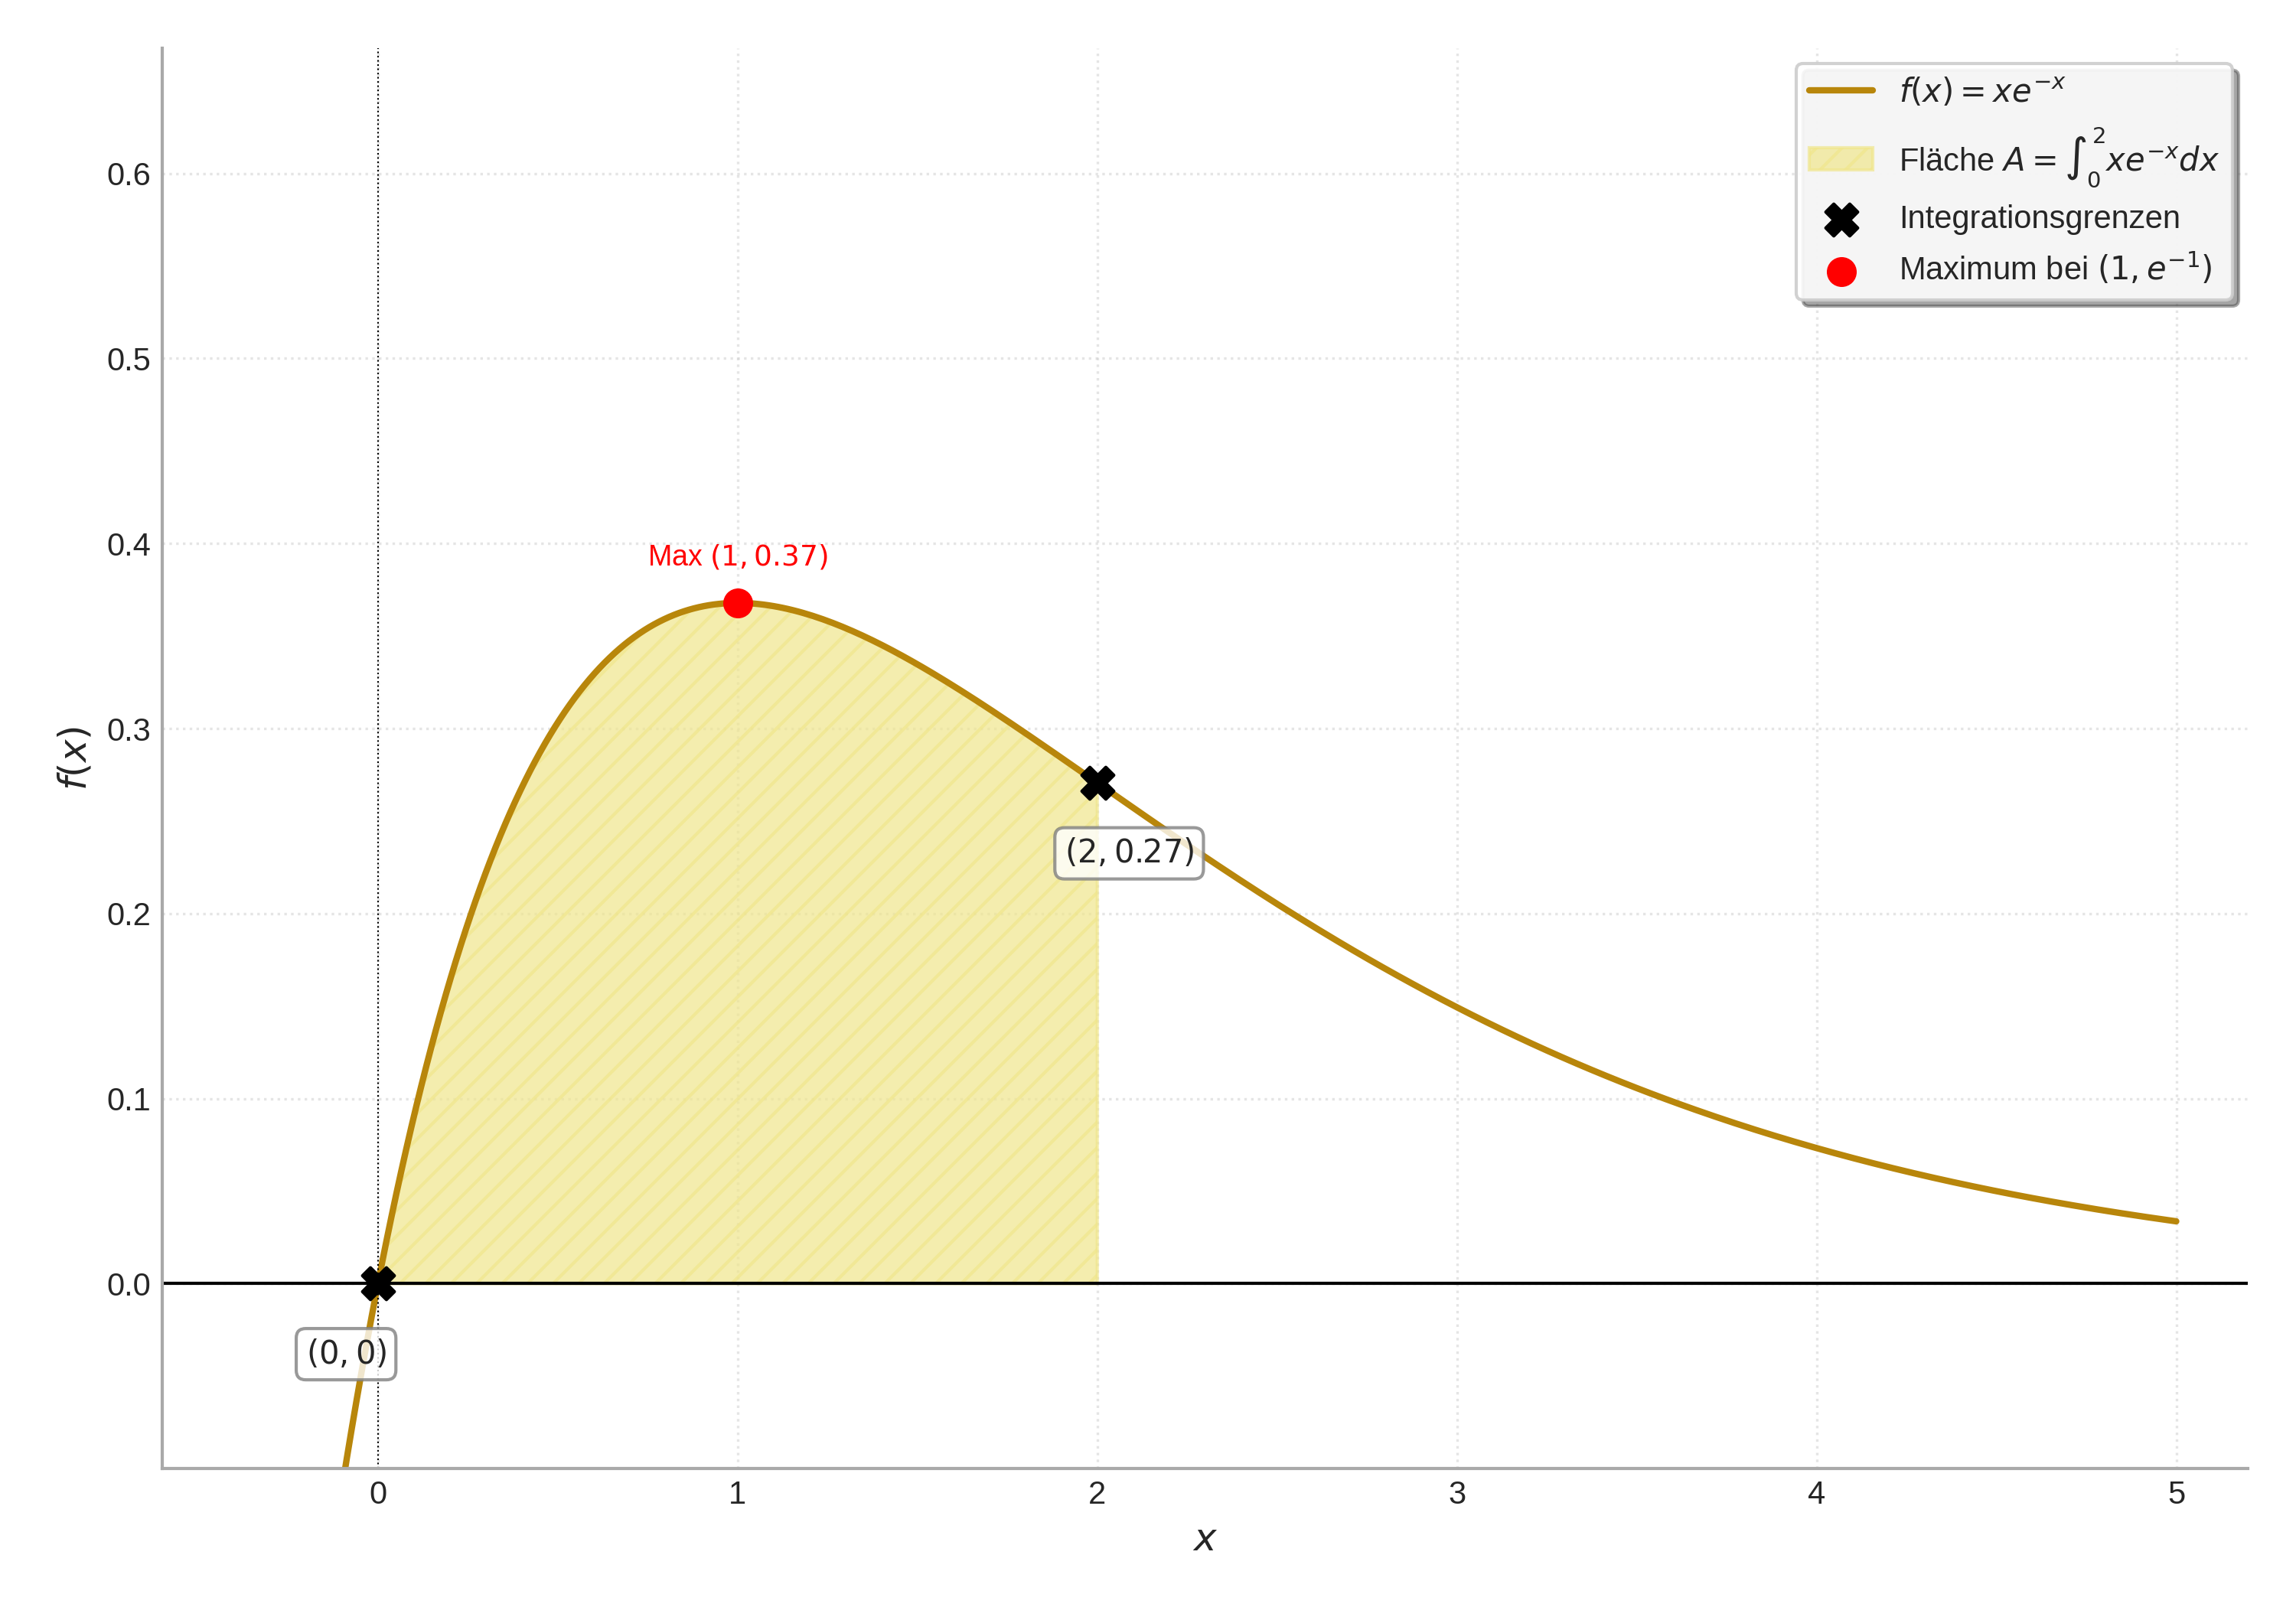
\includegraphics[width=0.8\textwidth]{grafiken/Integral_Flaeche_xehochminusx.png}
    \captionof{figure}{Fläche unter $f(x)=xe^{-x}$}
    \label{fig:flaeche_xehochminusx}
\end{center}
\end{aufgabenumgebung}

% Vorheriger Inhalt des Kapitels bis zur aufgabenumgebung 'Tangentenprobleme an einer kubischen Funktion'
% ... (siehe vorherige Canvas-Version) ...
\subsubsection{Weitere anspruchsvolle Aufgaben mit Exponentialfunktionen}
\label{subsubsec:exp_anwendungen_vertiefung_neu}

Die folgenden Aufgaben kombinieren die Ableitung von Exponentialfunktionen mit den Konzepten der Kurvendiskussion und Anwendungen. Sie erfordern oft mehrere Ableitungsregeln und ein gutes Verständnis der Zusammenhänge.

\begin{aufgabenumgebung}{Optimierung im biologischen Kontext – Wachstum und Hemmung}
Eine Bakterienpopulation wächst zunächst, wird aber durch einen hemmenden Faktor (z.B. begrenzte Nährstoffe) beeinflusst. Die Anzahl der Bakterien $N$ (in Tausend) nach $t$ Stunden kann modelliert werden durch die Funktion:
\[ N(t) = 5t \cdot e^{-0.1t} \quad (\text{für } t \ge 0) \]
\begin{enumerate}
    \item \textbf{Anfangsbestand:} Wie viele Bakterien sind zum Zeitpunkt $t=0$ vorhanden? Interpretiere das Ergebnis im Kontext.
    \item \textbf{Wachstumsrate:} Bestimme die Funktion $N'(t)$, welche die Wachstumsrate der Bakterienpopulation zum Zeitpunkt $t$ angibt. (Produkt- und Kettenregel sind hier gefragt!)
    \item \textbf{Maximale Population:}
        \begin{itemize}
            \item Zu welchem Zeitpunkt $t_{max}$ erreicht die Bakterienpopulation ihr Maximum? (Tipp: Notwendige Bedingung für Extremstellen $N'(t)=0$. Da $e^{-0.1t}$ nie Null wird, musst du nur den anderen Faktor betrachten.)
            \item Überprüfe mit der zweiten Ableitung $N''(t)$ oder dem Vorzeichenwechselkriterium von $N'(t)$, ob es sich tatsächlich um ein Maximum handelt.
            \item Wie groß ist die maximale Bakterienpopulation $N(t_{max})$?
        \end{itemize}
    \item \textbf{Verhalten für $t \to \infty$:} Was passiert mit der Bakterienpopulation für sehr große Zeiten? (Untersuche $\lim_{t \to \infty} N(t)$). Ist das biologisch sinnvoll?
    \item \textbf{Stärkste Zunahme/Abnahme der Wachstumsrate (für Experten):}
        Die Änderungsrate der Wachstumsrate wird durch $N''(t)$ beschrieben. Wann ist die Zunahme der Wachstumsrate maximal (d.h. wann wächst die Population am schnellsten schneller)? Wann ist die Abnahme der Wachstumsrate maximal (d.h. wann verlangsamt sich das Wachstum am stärksten)? (Tipp: Untersuche $N''(t)$ auf Extremstellen, d.h. bilde $N'''(t)$).
    \item \textbf{Skizze:} Skizziere den Graphen von $N(t)$ für $t \ge 0$ und markiere den maximalen Bestand.
\end{enumerate}
\end{aufgabenumgebung}


\subsubsection{Anwendungen der Integralrechnung auf Exponentialfunktionen}
\label{subsubsec:exp_integration_anwendungen}

Nachdem wir gelernt haben, wie man Exponentialfunktionen ableitet und ihre Graphen analysiert, wollen wir nun unser Wissen über die Integralrechnung anwenden. Insbesondere die Berechnung von Flächeninhalten, die von Exponentialfunktionen begrenzt werden, oder die Rekonstruktion von Gesamtbeständen aus exponentiellen Änderungsraten sind wichtige Anwendungen.

Erinnerung an die Stammfunktionen:
\begin{itemize}
    \item $\int e^x \,dx = e^x + C$
    \item $\int e^{kx} \,dx = \frac{1}{k} e^{kx} + C$ (für $k \neq 0$)
    \item Für Produkte wie $x \cdot e^x$ oder $x^2 \cdot e^x$ benötigen wir die partielle Integration.
    \item Für verkettete Funktionen im Exponenten, wie $e^{x^2}$, benötigen wir oft die Substitution (wenn der Faktor $g'(x)$ vorhanden ist).
\end{itemize}

\begin{aufgabenumgebung}{Flächenberechnung mit Exponentialfunktionen}
\begin{enumerate}
    \item \textbf{Fläche unter $e^x$:}
        Berechne den Inhalt der Fläche, die vom Graphen der Funktion $f(x) = e^x$, der x-Achse und den Geraden $x=0$ und $x=2$ eingeschlossen wird. Fertige eine Skizze an und markiere die Fläche.
    \item \textbf{Fläche unter $e^{-x}$:}
        Berechne den Inhalt der Fläche, die vom Graphen der Funktion $g(x) = 2e^{-0.5x}$, der x-Achse und den Geraden $x=0$ und $x=4$ eingeschlossen wird. Skizziere auch hier den Graphen und die Fläche.
    \item \textbf{Fläche zwischen $e^x$ und einer Geraden (für Experten):}
        Die Graphen der Funktionen $f(x) = e^x$ und $h(x) = e\cdot x + 1$ schließen eine Fläche ein.
        \begin{itemize}
            \item Zeige, dass sich die Graphen an der Stelle $x=0$ und $x=1$ schneiden.
            \item Bestimme, welche Funktion im Intervall $[0,1]$ oben bzw. unten liegt.
            \item Berechne den Inhalt der eingeschlossenen Fläche.
                \begin{center}
                    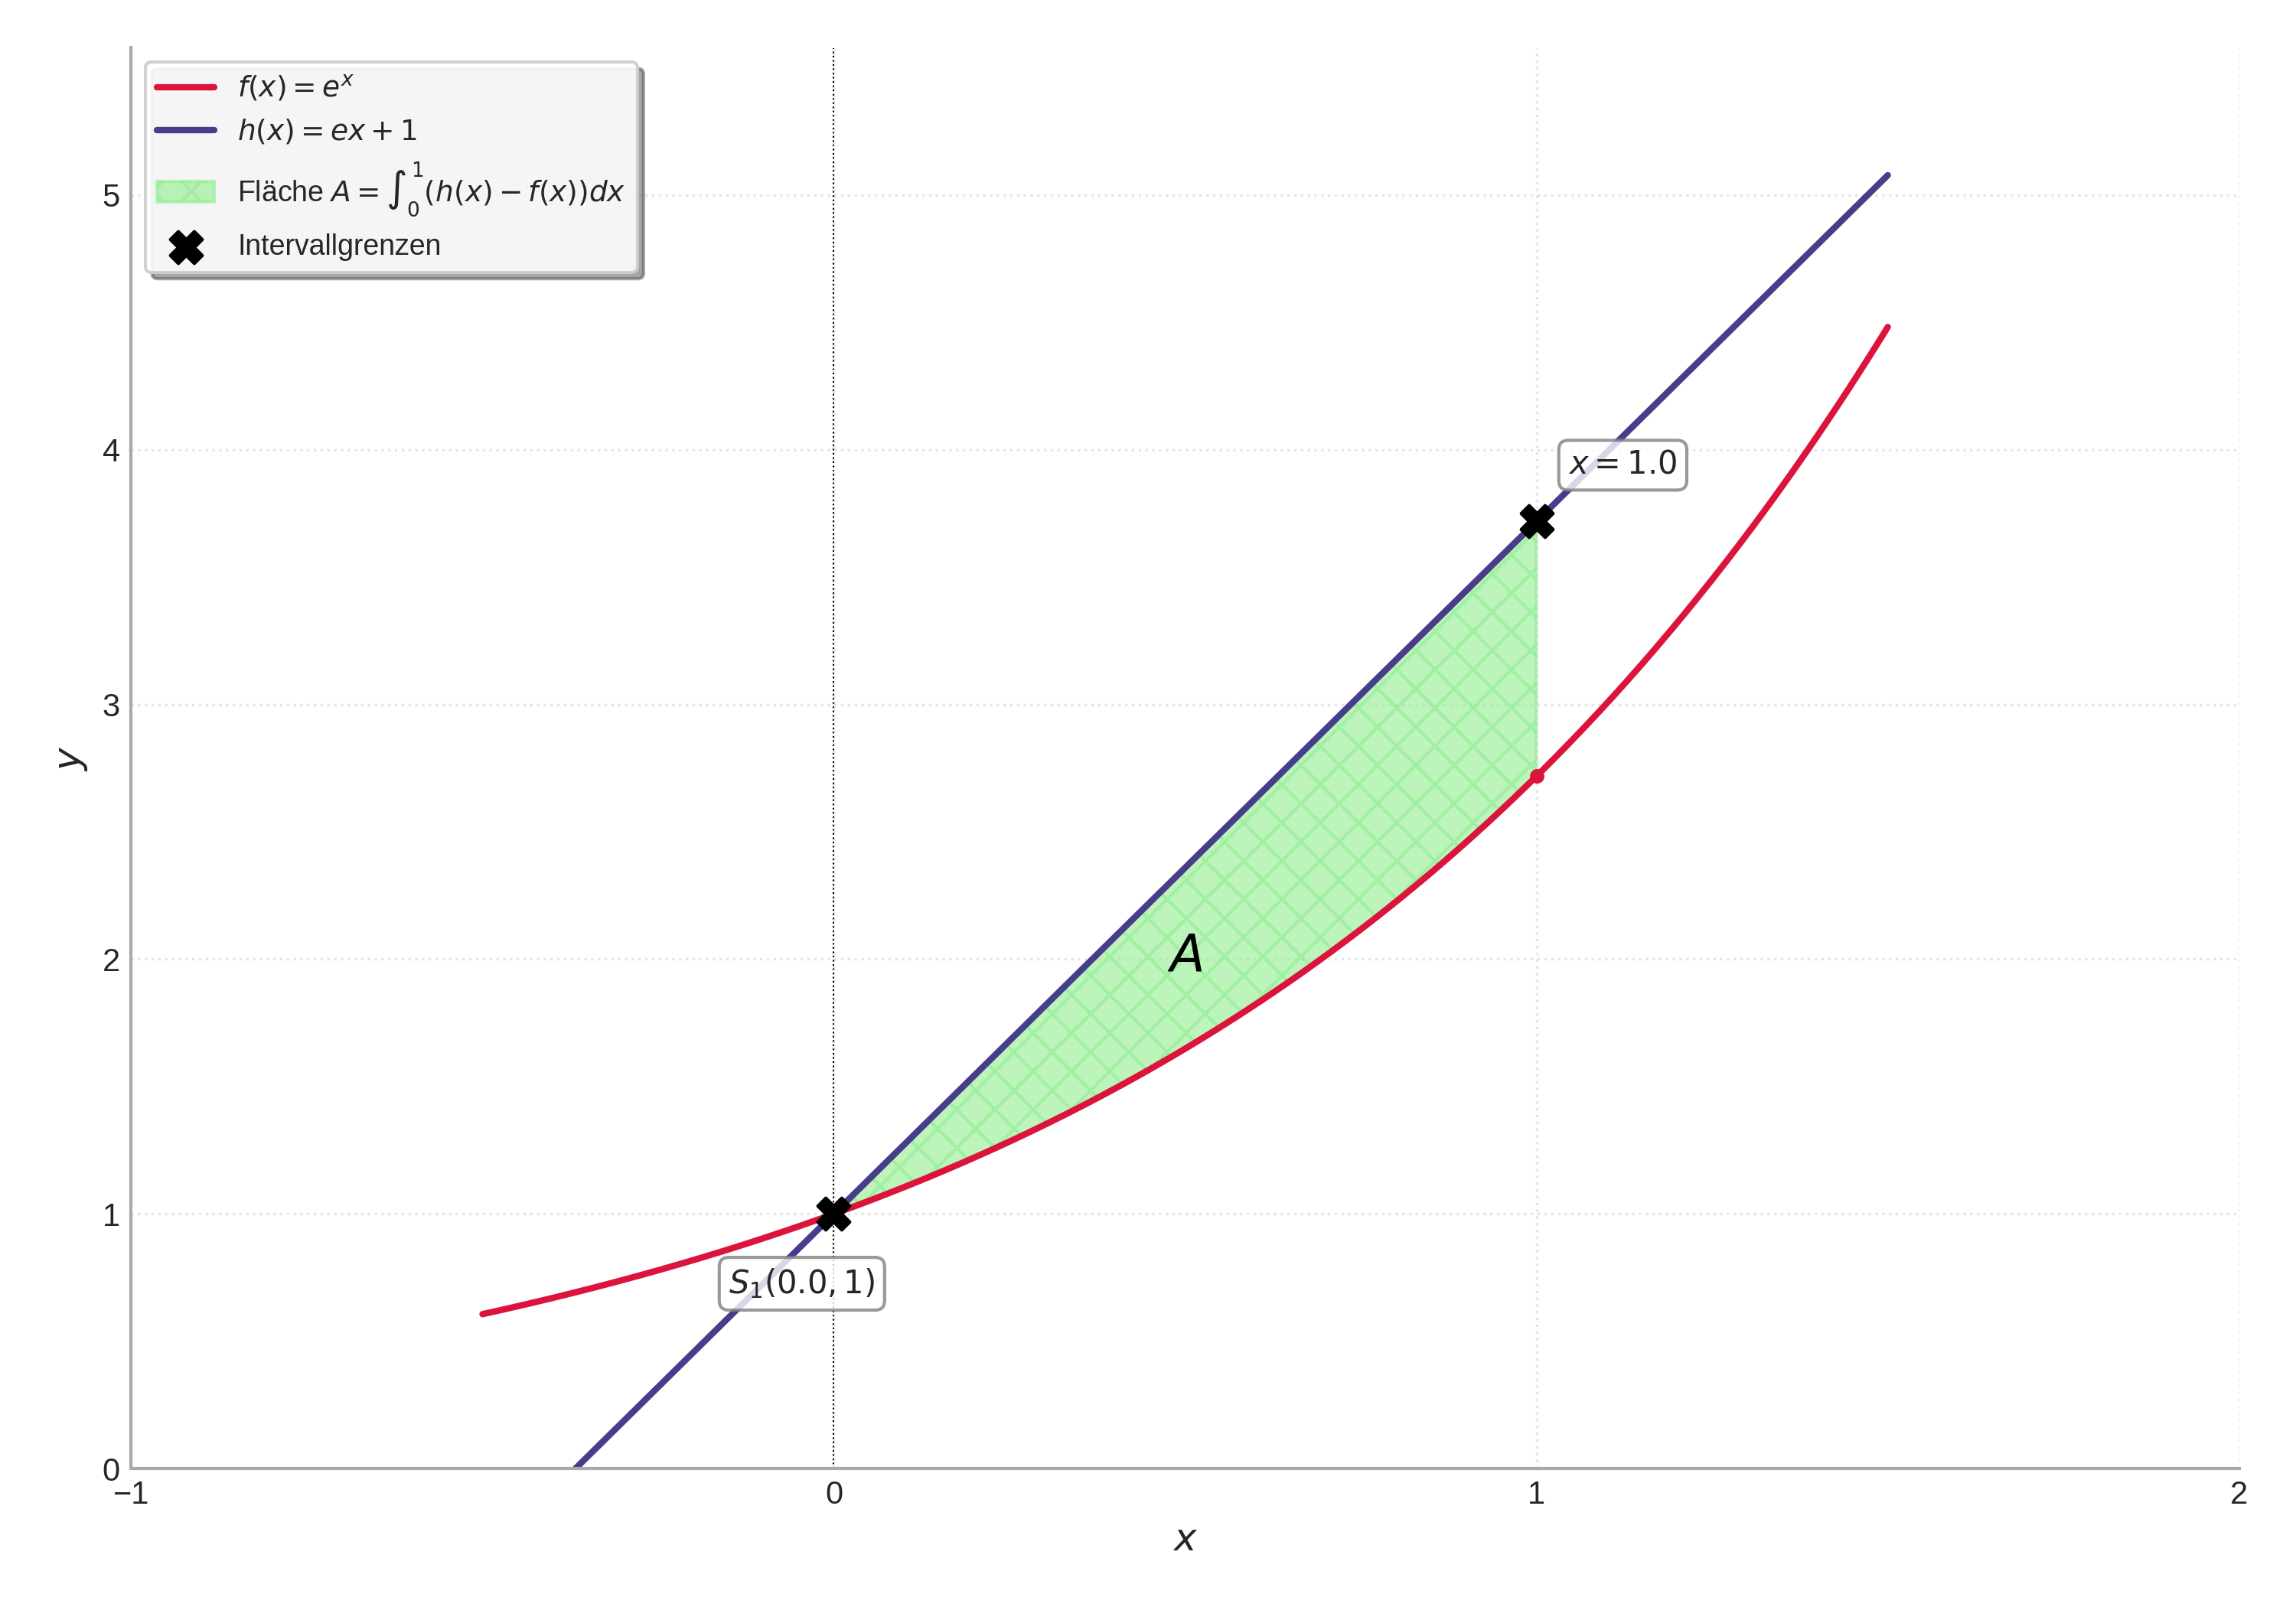
\includegraphics[width=0.8\textwidth]{grafiken/Integral_Flaeche_ex_Gerade.png}
                    \captionof{figure}{Fläche zwischen $f(x)=e^x$ und $h(x)=ex+1$}
                    \label{fig:flaeche_ex_gerade}
                \end{center}
        \end{itemize}
\end{enumerate}
\end{aufgabenumgebung}

\begin{aufgabenumgebung}{Anwendung: Medikamentenabbau im Körper}
Die Konzentration eines Medikaments im Blut eines Patienten (in mg/Liter) kann nach der Einnahme durch die Funktion $K(t) = 10 \cdot t \cdot e^{-0.2t}$ beschrieben werden, wobei $t$ die Zeit in Stunden nach der Einnahme ist ($t \ge 0$).
\begin{enumerate}
    \item Zu welchem Zeitpunkt ist die Konzentration des Medikaments maximal? Wie hoch ist diese maximale Konzentration? (Nutze die Differentialrechnung).
    \item Die 'Gesamtwirkung' eines Medikaments über einen bestimmten Zeitraum kann manchmal durch das Integral der Konzentrationsfunktion über diesen Zeitraum angenähert werden (dies ist eine Vereinfachung, aber das Integral gibt eine Art 'kumulierte Dosis' an).
        Berechne $\int_0^{10} K(t) \,dt$. (Tipp: Partielle Integration ist hier notwendig! Wähle $u'(t)=e^{-0.2t}$ und $v(t)=10t$).
        Was könnte dieser Wert im Kontext bedeuten?
    \item (Für Experten): Was ist $\lim_{t \to \infty} K(t)$? Was bedeutet das für die Konzentration des Medikaments nach sehr langer Zeit?
\end{enumerate}
\end{aufgabenumgebung}

\begin{aufgabenumgebung}{Uneigentliches Integral – Fläche bis ins Unendliche?}
Wir betrachten die Funktion $f(x) = e^{-x}$ für $x \ge 0$.
\begin{enumerate}
    \item Skizziere den Graphen von $f(x)$.
    \item Berechne den Flächeninhalt $A_b = \int_0^b e^{-x} \,dx$ für eine beliebige obere Grenze $b > 0$.
    \item Was passiert mit diesem Flächeninhalt $A_b$, wenn $b$ unendlich groß wird? Berechne also den Grenzwert $\lim_{b \to \infty} A_b$.
    \begin{tippumgebung}{Uneigentliches Integral}
    Ein Integral der Form $\int_a^\infty f(x) \,dx$ nennt man ein \textbf{uneigentliches Integral}. Man berechnet es als Grenzwert:
    \[ \int_a^\infty f(x) \,dx = \lim_{b \to \infty} \int_a^b f(x) \,dx \]
    Wenn dieser Grenzwert existiert (also eine endliche Zahl ist), sagt man, das uneigentliche Integral \textbf{konvergiert}. Ansonsten \textbf{divergiert} es.
    \end{tippumgebung}
    \item Kann eine Fläche, die sich ins Unendliche erstreckt, einen endlichen Inhalt haben? Diskutiere dein Ergebnis aus c).
\end{enumerate}
\end{aufgabenumgebung}



\begin{aufgabenumgebung}{Exponentialfunktionen – Übergreifende und anspruchsvolle Aufgaben}
Die folgenden Aufgaben sollen dein Verständnis für Exponentialfunktionen, ihre Ableitungen, Stammfunktionen und Anwendungen umfassend prüfen. Versuche, die Aufgaben sorgfältig und schrittweise zu lösen.
\begin{enumerate}
    \item \textbf{Kurvendiskussion einer e-Funktion mit Polynomfaktor:}
        Führe eine vollständige Kurvendiskussion für die Funktion $f(x) = (4-x^2)e^{-0.5x}$ durch. Untersuche dabei insbesondere:
        \begin{itemize}
            \item Definitionsbereich und Symmetrie.
            \item Verhalten im Unendlichen und Asymptoten. (Tipp: $\lim_{x\to\infty} x^n e^{-kx} = 0$ für $k>0$).
            \item Nullstellen.
            \item Extrempunkte (Lage und Art).
            \item Wendepunkte (Lage und Krümmungsverhalten).
            \item Skizziere den Graphen von $f(x)$.
        \end{itemize}

    \item \textbf{Optimierung: Maximale Konzentration eines Medikaments}
        Die Konzentration $K(t)$ eines Medikaments im Blut eines Patienten (in mg/l) zum Zeitpunkt $t$ (in Stunden nach Einnahme) wird durch die Funktion $K(t) = 20t \cdot e^{-0.25t}$ für $t \ge 0$ beschrieben.
        \begin{itemize}
            \item Zu welchem Zeitpunkt $t_{max}$ erreicht die Konzentration des Medikaments ihr Maximum?
            \item Wie hoch ist diese maximale Konzentration?
            \item Bestimme die Funktion $K'(t)$, die die Änderungsrate der Konzentration angibt. Wann nimmt die Konzentration am stärksten zu? (Suche nach dem Maximum von $K'(t)$, also einem Wendepunkt von $K(t)$ mit bestimmten Eigenschaften).
        \end{itemize}

    \item \textbf{Flächenberechnung und uneigentliches Integral:}
        Gegeben ist die Funktion $f(x) = (x+1)e^{-x}$.
        \begin{itemize}
            \item Bestimme die Stammfunktion $F(x)$ von $f(x)$ mithilfe partieller Integration.
            \item Berechne den Inhalt der Fläche, die der Graph von $f(x)$ mit der x-Achse und der y-Achse im ersten Quadranten einschließt. (Finde dazu die Nullstelle von $f(x)$ für $x \ge 0$).
            \item (Für Experten): Untersuche, ob die Fläche, die der Graph von $f(x)$ mit der x-Achse für $x \ge 0$ einschließt, einen endlichen Inhalt hat. Berechne dazu das uneigentliche Integral $\int_0^\infty (x+1)e^{-x} \,dx = \lim_{b \to \infty} \int_0^b (x+1)e^{-x} \,dx$.
        \end{itemize}
            \begin{center}
                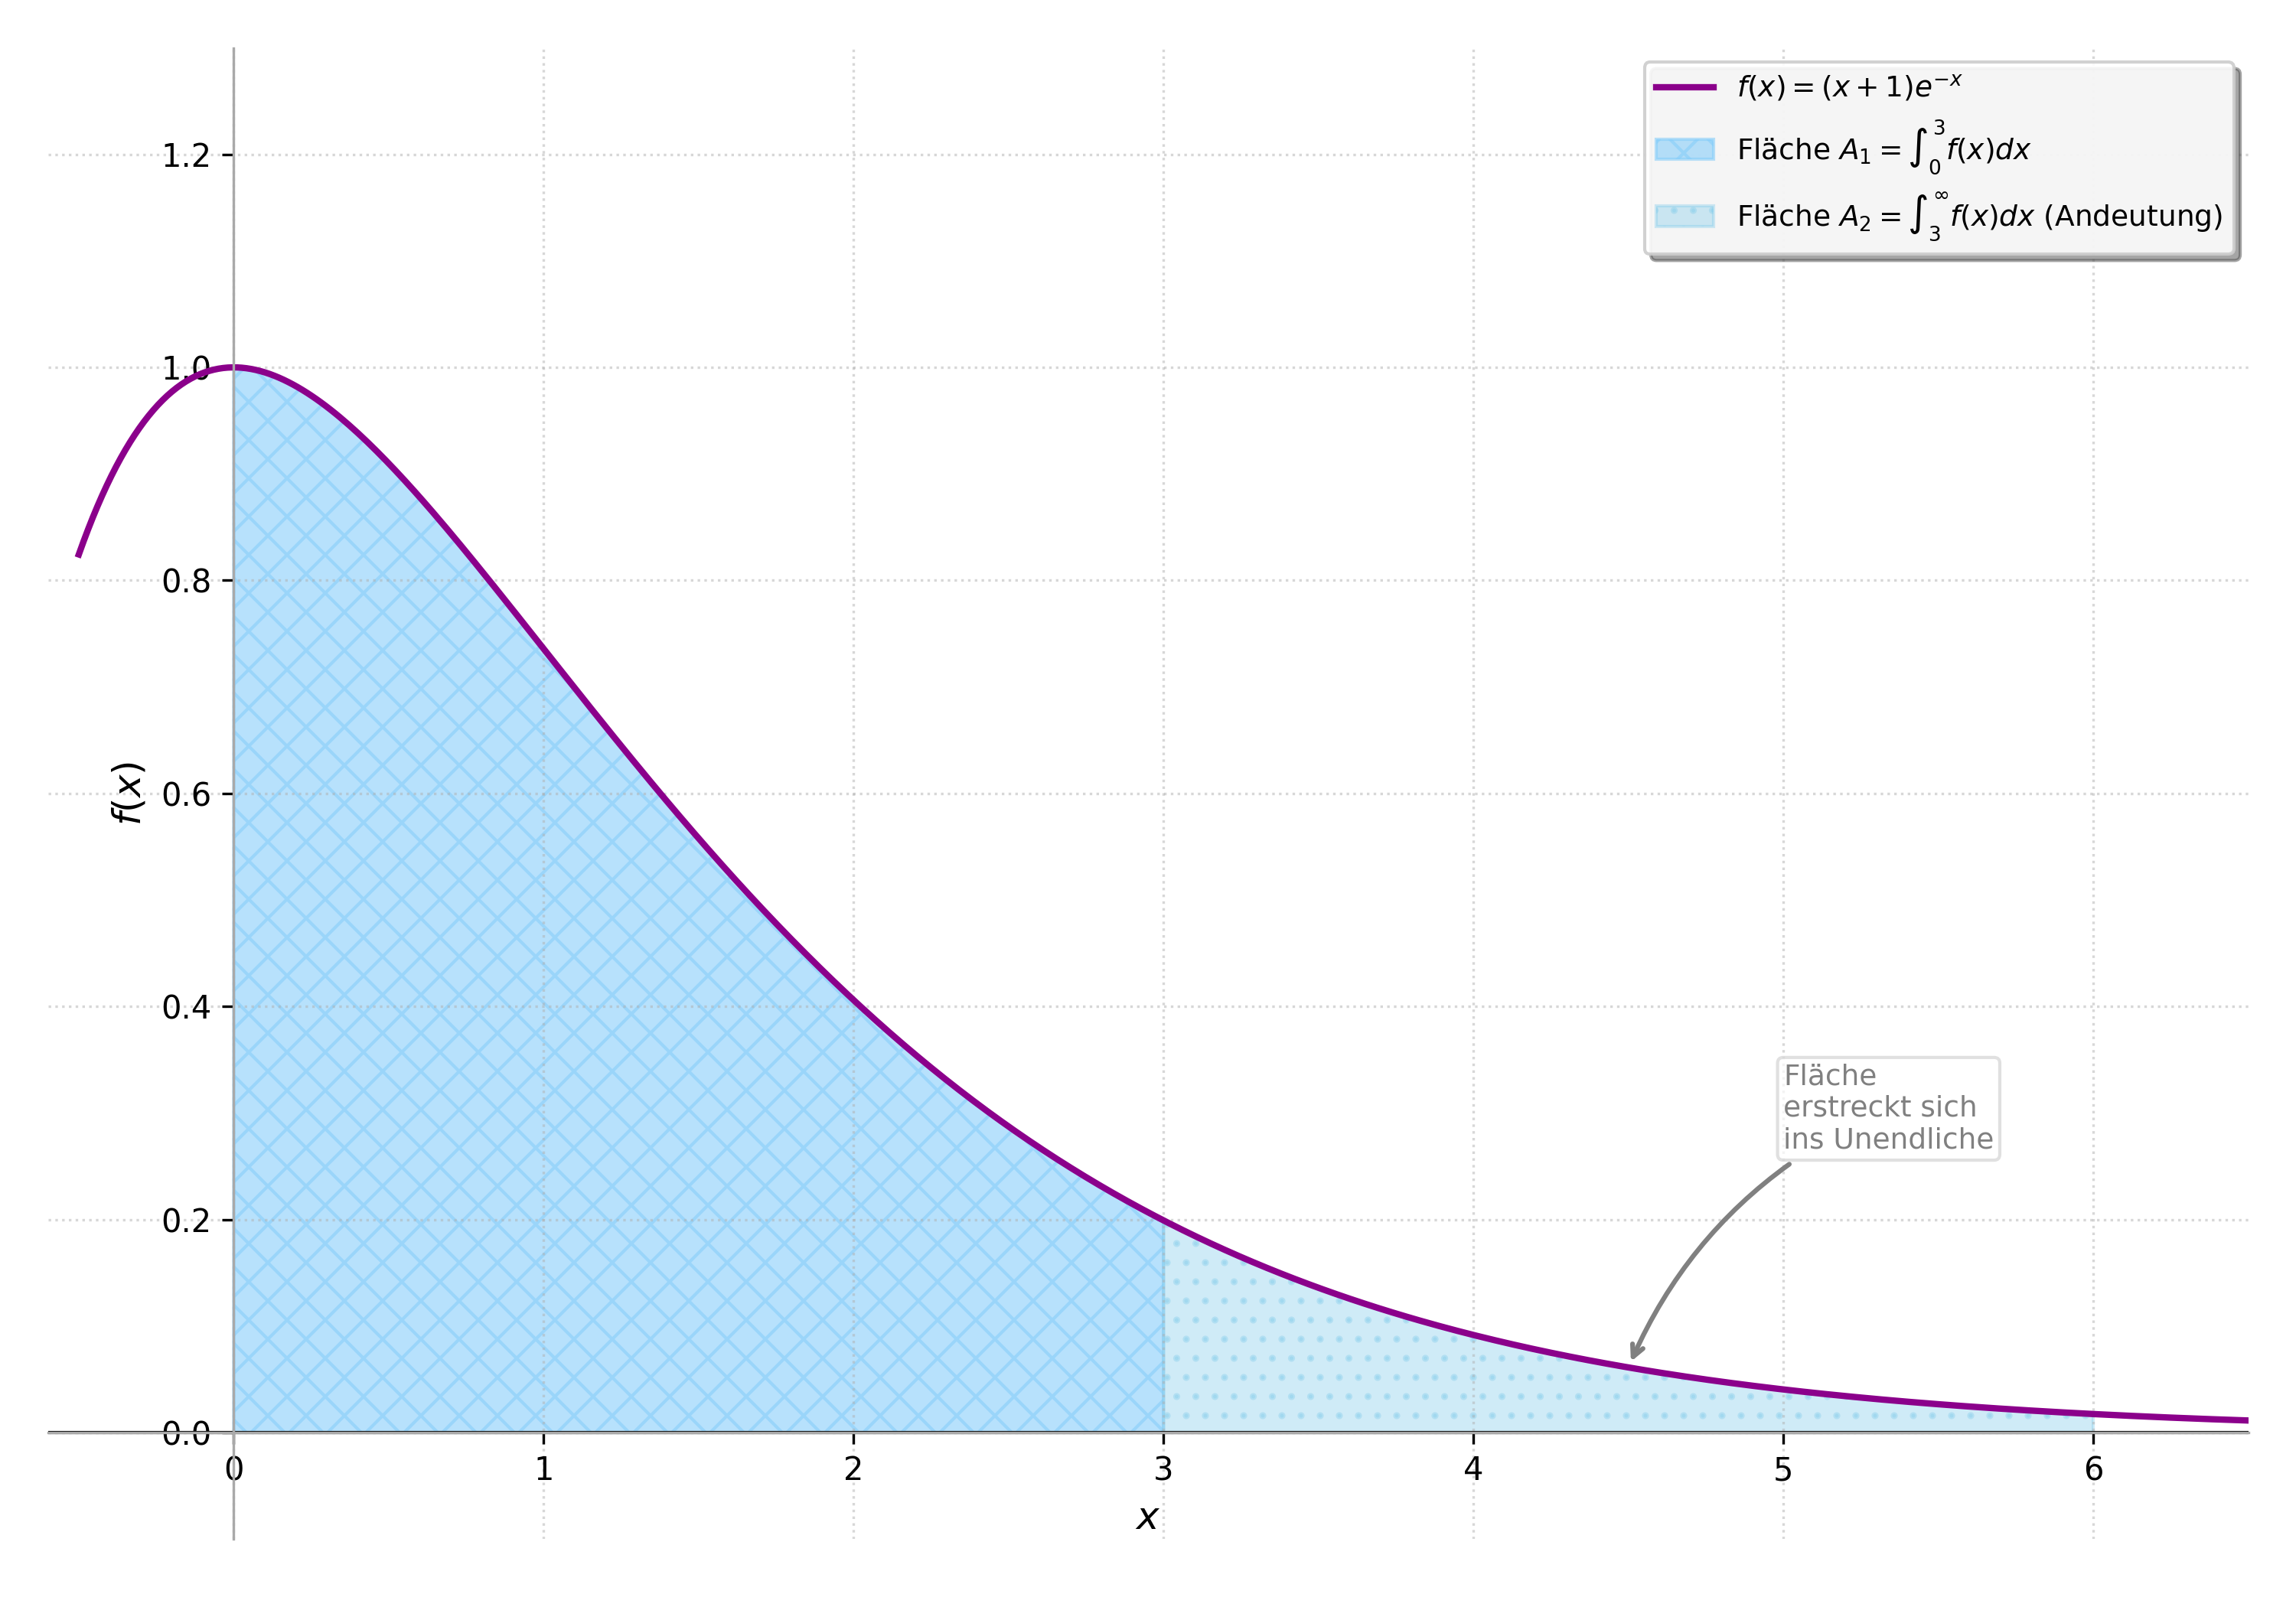
\includegraphics[width=0.8\textwidth]{grafiken/Integral_Flaeche_xplus1ehochminusx.png}
                \captionof{figure}{Fläche unter $f(x)=(x+1)e^{-x}$}
                \label{fig:flaeche_xplus1ehochminusx}
            \end{center}
            
    \item \textbf{Rekonstruktion einer Exponentialfunktion und Tangente:}
        Eine Funktion $f$ ist gegeben durch $f(x) = (ax+b)e^{-x}$. Der Graph von $f$ hat im Punkt $P(0|2)$ eine Tangente, die parallel zur Geraden $y=3x-5$ ist.
        \begin{itemize}
            \item Bestimme die Werte der Parameter $a$ und $b$.
            \begin{tippumgebung}{Bedingungen aufstellen}
            'Graph geht durch $P(0|2)$' $\implies f(0)=2$.
            'Tangente in $P(0|2)$ parallel zu $y=3x-5$' $\implies f'(0) = 3$.
            Bilde $f'(x)$ mit der Produkt- und Kettenregel.
            \end{tippumgebung}
            \item Bestimme die Gleichung der Tangente an den Graphen von $f$ im Punkt $P(0|2)$.
            \item Untersuche die Funktion $f(x)$ mit den gefundenen Parametern auf Nullstellen und Extrempunkte.
        \end{itemize}

    \item \textbf{Schar von Exponentialfunktionen (Schwer):}
        Gegeben ist die Funktionenschar $f_k(x) = x^2 e^{kx}$ mit dem Scharparameter $k \in \mathbb{R}$, $k \neq 0$.
        \begin{itemize}
            \item Bestimme die Nullstellen von $f_k(x)$.
            \item Bestimme die erste Ableitung $f_k'(x)$. Für welche Werte von $x$ (in Abhängigkeit von $k$) ist $f_k'(x)=0$?
            \item Untersuche die Art der Extremstellen in Abhängigkeit von $k$. (Tipp: Betrachte die Fälle $k>0$ und $k<0$ getrennt für das Verhalten der zweiten Ableitung oder den Vorzeichenwechsel der ersten Ableitung).
            \item Gibt es Werte für $k$, sodass die Funktion keine Extrempunkte besitzt?
        \end{itemize}
\end{enumerate}
\end{aufgabenumgebung}


\begin{kurzknappumgebung}{Exponentialfunktionen – Das Wichtigste im Überblick}
\begin{itemize}
    \item \textbf{Die natürliche Exponentialfunktion $f(x)=e^x$:}
        \begin{itemize}
            \item Basis $e \approx 2,71828\dots$ (Eulersche Zahl).
            \item Definitionsbereich $D_f = \mathbb{R}$, Wertebereich $W_f = (0, \infty)$.
            \item Keine Nullstellen, y-Achsenabschnitt bei $(0|1)$.
            \item Streng monoton steigend, linksgekrümmt.
            \item $\lim_{x \to -\infty} e^x = 0$ (horizontale Asymptote $y=0$), $\lim_{x \to \infty} e^x = \infty$.
            \item Besondere Eigenschaft: $(e^x)' = e^x$ und $\int e^x \,dx = e^x + C$.
        \end{itemize}
    \item \textbf{Transformierte Exponentialfunktion $f(x) = a \cdot e^{k(x-c)} + d$:}
        \begin{itemize}
            \item Parameter $a, k, c, d$ bewirken Streckung/Stauchung, Spiegelung, Verschiebung.
            \item Ableitung $(e^{kx})' = k \cdot e^{kx}$. Stammfunktion $\int e^{kx} \,dx = \frac{1}{k}e^{kx} + C$.
        \end{itemize}
    \item \textbf{Allgemeine Exponentialfunktion $f(x) = b^x$ ($b>0, b\neq 1$):}
        \begin{itemize}
            \item Umwandelbar zu $b^x = e^{x \ln(b)}$.
            \item Ableitung $(b^x)' = b^x \cdot \ln(b)$.
            \item Stammfunktion $\int b^x \,dx = \frac{1}{\ln(b)}b^x + C$.
        \end{itemize}
    \item \textbf{Anwendung der Ableitungsregeln:} Produkt-, Quotienten- und Kettenregel sind essentiell für Kombinationen von $e^x$ mit Polynomen oder anderen Funktionen (z.B. $f(x) = P(x) \cdot e^{g(x)}$).
    \item \textbf{Nullstellen von $P(x) \cdot e^{g(x)}$:} Da $e^{g(x)}$ immer positiv ist, hängen die Nullstellen nur von den Nullstellen des Faktors $P(x)$ ab.
    \item \textbf{Grenzwerte:} Die $e$-Funktion 'dominiert' oft Polynome im Unendlichen (z.B. $\lim_{x\to\infty} x^n e^{-kx} = 0$ für $k>0$).
    \item \textbf{Kurvendiskussion:} Folgt den bekannten Schritten, wobei die speziellen Eigenschaften von $e^x$ (keine Nullstellen, immer positiv, Grenzwertverhalten) und die Ableitungsregeln berücksichtigt werden.
    \item \textbf{Integrationstechniken mit $e^x$:}
        \begin{itemize}
            \item Partielle Integration für Produkte wie $\int x e^x \,dx$.
            \item Integration durch Substitution für verkettete Funktionen wie $\int 2x e^{x^2} \,dx$.
        \end{itemize}
    \item \textbf{Anwendungen:} Beschreibung von Wachstums- und Zerfallsprozessen, Flächenberechnungen, Mittelwerte, uneigentliche Integrale.
\end{itemize}
\end{kurzknappumgebung}

\begin{infoboxumgebung}{Ausblick: Logarithmusfunktionen – Die andere Seite der Medaille}
Mit den Exponentialfunktionen hast du eine unglaublich mächtige Funktionsklasse kennengelernt, die in unzähligen Bereichen der Wissenschaft und des Alltags Anwendung findet. Sie beschreiben Prozesse, bei denen sich etwas proportional zu seinem aktuellen Bestand ändert – das klassische Merkmal von Wachstum und Zerfall.

Doch was, wenn wir die umgekehrte Frage stellen? Wenn wir wissen, wie groß ein Bestand ist, und wissen wollen, wie viel Zeit vergangen ist? Oder wenn wir eine Gleichung wie $e^x = 100$ nach $x$ auflösen wollen? Hier kommt die \textbf{Logarithmusfunktion} ins Spiel, insbesondere der \textbf{natürliche Logarithmus ($\ln x$)}, der die direkte Umkehrfunktion zur natürlichen Exponentialfunktion $e^x$ ist.

Im nächsten Kapitel werden wir uns genau diese Logarithmusfunktionen ansehen:
\begin{itemize}
    \item Wie sind sie definiert und welche Eigenschaften haben sie?
    \item Wie sehen ihre Graphen aus (Tipp: Spiegelung von $e^x$ an $y=x$)?
    \item Wie leitet man Logarithmusfunktionen ab und wie bildet man ihre Stammfunktionen?
    \item Wie können wir sie in Kurvendiskussionen und Anwendungsaufgaben nutzen?
\end{itemize}
Du wirst sehen, dass Exponential- und Logarithmusfunktionen wie zwei Seiten derselben Medaille sind und zusammen ein unschlagbares Team bilden, um eine riesige Bandbreite an Problemen zu lösen. Die Werkzeuge der Differential- und Integralrechnung werden uns auch hier treue Dienste leisten.
\end{infoboxumgebung}


\begin{aufgabenumgebung}{Checkliste: Die Exponentialfunktion im Kern verstehen}
Die Exponentialfunktion ist in vielerlei Hinsicht besonders. Diese Fragen helfen dir, dein Verständnis zu vertiefen:

\begin{enumerate}[label=(\alph*)]
    \item \textbf{Die Eulersche Zahl $e$ und die natürliche Exponentialfunktion:}
    \begin{itemize}
        \item Warum wird $f(x)=e^x$ als die 'natürliche' Exponentialfunktion bezeichnet? Welche einzigartige Eigenschaft hat ihre Ableitung, und was bedeutet das für die Steigung ihres Graphen an jeder Stelle $x$?
        \item Vergleiche die Graphen von $y=2^x$, $y=e^x$ und $y=3^x$ in einer Skizze. Wo schneiden sie die y-Achse? Welche Funktion wächst für $x>0$ am schnellsten, welche am langsamsten? Wie verhält es sich mit ihren Steigungen an der Stelle $x=0$?
    \end{itemize}
    \item \textbf{Transformationen und Asymptoten:}
    Betrachte die Funktion $g(x) = A \cdot e^{k(x-B)} + C$.
    \begin{itemize}
        \item Erkläre, wie sich die Parameter $A, k, B, C$ jeweils auf den Graphen der Grundfunktion $y=e^x$ auswirken (Streckung, Stauchung, Spiegelung, Verschiebung).
        \item Welche Gleichung hat die waagerechte Asymptote von $g(x)$? Wie hängt diese vom Parameter $C$ ab? Warum kann der Graph diese Asymptote nie schneiden, wenn $A \neq 0$?
        \item Wenn $A>0$ und $k>0$: Ist die Funktion streng monoton steigend oder fallend? Was passiert, wenn $k<0$ ist?
    \end{itemize}
    \item \textbf{Von $b^x$ zu $e^{kx}$:}
    \begin{itemize}
        \item Erkläre mit eigenen Worten, warum jede Exponentialfunktion $f(x)=b^x$ (mit $b>0, b\neq1$) auch in der Form $f(x)=e^{kx}$ geschrieben werden kann. Welchen Wert hat $k$ in diesem Fall?
        \item Nutze diese Umschreibung, um die Ableitungsregel $(b^x)' = b^x \ln(b)$ aus der Regel $(e^{kx})' = k e^{kx}$ herzuleiten.
    \end{itemize}
    \item \textbf{Grenzwertverhalten und Dominanz:}
    \begin{itemize}
        \item Warum ist $\lim_{x \to -\infty} e^x = 0$, aber $\lim_{x \to \infty} e^x = \infty$?
        \item Betrachte eine Funktion $h(x) = x^n \cdot e^{-x}$ (mit $n \in \mathbb{N}$). Warum ist $\lim_{x \to \infty} h(x) = 0$, obwohl $x^n$ gegen $\infty$ geht? Welche Funktion 'dominiert' hier das Verhalten für große $x$?
    \end{itemize}
\end{enumerate}
\end{aufgabenumgebung}


\begin{aufgabenumgebung}{Checkliste: Exponentialfunktionen in der Analysis anwenden}
Die Analyse von Funktionen mit Exponentialtermen erfordert oft eine Kombination verschiedener Werkzeuge.

\begin{enumerate}[label=(\alph*)]
    \item \textbf{Nullstellen von $f(x) = P(x) \cdot e^{g(x)}$:}
    Wenn du die Nullstellen einer Funktion suchen sollest, die ein Produkt aus einem Polynom $P(x)$ und einem Exponentialterm $e^{g(x)}$ ist:
    \begin{itemize}
        \item Warum kannst du dich bei der Nullstellensuche ausschließlich auf den Faktor $P(x)$ konzentrieren?
        \item Gilt eine ähnliche Regel auch für die Nullstellensuche der Ableitung $f'(x)$ solcher Funktionen? (Tipp: Leite $P(x)e^{g(x)}$ allgemein mit Produkt- und Kettenregel ab und schaue, ob du $e^{g(x)}$ ausklammern kannst).
    \end{itemize}
    \item \textbf{Extremwertbestimmung bei $e$-Funktionen:}
    Betrachte die Funktion $f(x) = x^2 e^{-x}$.
    \begin{itemize}
        \item Welche Ableitungsregeln benötigst du, um $f'(x)$ und $f''(x)$ zu bilden?
        \item Wie gehst du vor, um die lokalen Extrempunkte zu finden? Erkläre die notwendige und die hinreichende Bedingung.
        \item Was erwartest du für das Verhalten von $f(x)$ für $x \to \infty$ und $x \to -\infty$? Wie hilft dir das, deine gefundenen Extrema einzuordnen (lokal vs. global)?
    \end{itemize}
    \item \textbf{Integrationstechniken im Kontext von $e$-Funktionen:}
    \begin{itemize}
        \item Für das Integral $\int (2x) e^{x^2} dx$: Welche Integrationstechnik bietet sich hier an und warum? Identifiziere die 'innere Funktion' und ihre Ableitung.
        \item Für das Integral $\int (x+1) e^x dx$: Welche Integrationstechnik ist hier typischerweise erfolgreich und warum? Wie würdest du die Faktoren für diese Technik wählen?
        \item Kannst du $\int e^{x^2} dx$ mit den in diesem Kapitel gelernten Methoden als elementare Funktion darstellen? (Tipp: Nicht jede Funktion hat eine einfach darstellbare Stammfunktion.)
    \end{itemize}
    \item \textbf{Interpretation im Anwendungskontext (Wachstum/Zerfall):}
    Ein Medikament wird im Körper exponentiell abgebaut, z.B. nach $M(t) = M_0 e^{-kt}$.
    \begin{itemize}
        \item Was bedeutet $M_0$ und was bedeutet ein größeres $k$ für den Abbauprozess?
        \item Die Ableitung $M'(t)$ gibt die momentane Abbaurate an. Ist $M'(t)$ positiv oder negativ? Warum ist das sinnvoll? Was passiert mit der Abbaurate für große $t$?
        \item Das bestimmte Integral $\int_{t_1}^{t_2} M(t) dt$ könnte als eine Art 'kumulierte Medikamentenbelastung' im Zeitintervall $[t_1, t_2]$ interpretiert werden. Welche Einheit hätte dieses Integral, wenn $M(t)$ in mg und $t$ in Stunden gemessen wird?
    \end{itemize}
\end{enumerate}
\end{aufgabenumgebung}

\begin{fehlerboxumgebung}{Interpretation von Grenzwerten und Asymptoten bei e-Funktionen}
Das Verhalten von Exponentialfunktionen im Unendlichen oder in Kombination mit Polynomen birgt einige Tücken:
\begin{itemize}
    \item \textbf{Asymptote bei $e^{kx}$ falsch bestimmt:} Die Funktion $f(x)=e^{kx}$ hat für $x \to -\infty$ die Asymptote $y=0$, wenn $k>0$ ist. Wenn aber $k<0$ (z.B. $f(x)=e^{-2x}$), dann gilt $\lim_{x \to \infty} e^{-2x} = 0$. Die Richtung, in der die x-Achse Asymptote ist, hängt vom Vorzeichen von $k$ ab! Bei $f(x)=A e^{k(x-B)} + C$ ist die Asymptote immer $y=C$.
    \item \textbf{Dominanz falsch eingeschätzt bei $P(x) \cdot e^{kx}$:} Für $x \to \infty$:
        \begin{itemize}
            \item Wenn $k>0$, 'gewinnt' der $e^{kx}$-Term gegen jedes Polynom $P(x)$, d.h. $P(x)e^{kx} \to \pm\infty$ (abhängig vom Vorzeichen von $P(x)$ für große $x$).
            \item Wenn $k<0$ (also $e^{-|k|x}$), 'gewinnt' der $e^{-|k|x}$-Term und geht schneller gegen 0, als $P(x)$ gegen $\infty$ geht. Also $P(x)e^{-|k|x} \to 0$.
        \end{itemize}
    Merke dir: Die Exponentialfunktion ist sehr 'stark' in ihrem Verhalten im Unendlichen.
    \item \textbf{Nullstellen von $P(x)e^{kx}$:} Die Nullstellen werden \textit{nur} durch $P(x)=0$ bestimmt, da $e^{kx}$ niemals Null wird. Manchmal wird fälschlicherweise versucht, $e^{kx}=0$ zu lösen.
\end{itemize}
Eine Skizze und die Betrachtung der Vorzeichen der beteiligten Faktoren helfen oft, Fehler zu vermeiden.
\end{fehlerboxumgebung}
\section{Logarithmusfunktionen – Die Welt des 'Zurückrechnens'}
\label{sec:logarithmusfunktionen_intro}

Nachdem wir die Exponentialfunktionen, insbesondere die natürliche Exponentialfunktion $f(x)=e^x$, kennengelernt haben, die uns exponentielles Wachstum und Zerfall beschreiben, wenden wir uns nun ihrer direkten 'Partnerin' zu: der \textbf{Logarithmusfunktion}.

\begin{tcolorbox}[colback=blue!5!white, colframe=blue!75!black, title=Was du in diesem Kapitel lernen wirst:]
Nachdem du dieses Kapitel durchgearbeitet hast, wirst du in der Lage sein:
\begin{itemize}[noitemsep, topsep=0pt, leftmargin=*, itemsep=2pt]
    \item den \textbf{Logarithmus} allgemein als Antwort auf die Frage nach dem Exponenten zu verstehen und den \textbf{natürlichen Logarithmus ($\ln x$)} als Umkehrfunktion der natürlichen Exponentialfunktion $e^x$ zu definieren und seine grundlegenden Eigenschaften (Graph, Definitions-/Wertebereich, Nullstelle, senkrechte Asymptote, Monotonie, Krümmung) zu beschreiben.
    \item die wichtigen \textbf{Logarithmengesetze} (für Produkte, Quotienten und Potenzen) sicher anzuwenden, um logarithmische Terme zu vereinfachen und Exponentialgleichungen nach der gesuchten Variablen aufzulösen.
    \item die \textbf{Ableitung} des natürlichen Logarithmus ($(\ln x)' = 1/x$) zu kennen und die Kettenregel zur Ableitung verketteter Logarithmusfunktionen ($(\ln(h(x)))' = \frac{h'(x)}{h(x)}$) sowie Produkt- und Quotientenregel auf Funktionen mit $\ln(x)$ anzuwenden.
    \item die \textbf{Stammfunktionen} $\int \frac{1}{x} \,dx = \ln|x|+C$ und $\int \ln(x) \,dx = x\ln(x) - x + C$ (letztere mithilfe partieller Integration) zu kennen und für Berechnungen zu nutzen.
    \item Integrale der wichtigen Form $\int \frac{g'(x)}{g(x)} \,dx = \ln|g(x)|+C$ zu erkennen und zu lösen (Integration durch Substitution).
    \item eine vollständige \textbf{Kurvendiskussion} für Funktionen durchzuführen, die den natürlichen Logarithmus enthalten (oft in Produkt- oder Quotientenform mit Polynomen), unter besonderer Berücksichtigung des Definitionsbereichs und relevanter Grenzwerte (z.B. $\lim_{x \to 0^+} x^n \ln x$).
    \item die Bedeutung und Anwendung des Logarithmus in verschiedenen Kontexten zu verstehen, beispielsweise beim Lösen von Exponentialgleichungen, die bei Wachstums- und Zerfallsprozessen auftreten, oder beim Verständnis logarithmischer Skalen.
\end{itemize}
Du wirst damit die wichtige 'Partnerfunktion' der Exponentialfunktion meistern und dein analytisches Repertoire zur Untersuchung und Beschreibung von Funktionen und realen Phänomenen entscheidend erweitern!
\end{tcolorbox}
\bigskip

Stell dir vor, du hast eine Exponentialgleichung wie $e^x = 10$. Wie findest du heraus, welchen Wert $x$ haben muss, damit diese Gleichung stimmt? Du suchst also den Exponenten, mit dem die Basis $e$ potenziert werden muss, um 10 zu erhalten. Genau diese Frage beantwortet uns der Logarithmus.

\begin{infoboxumgebung}{Was ist ein Logarithmus? Die Frage nach dem Exponenten!}
Der Logarithmus einer Zahl $y$ zu einer bestimmten Basis $b$ ist derjenige Exponent $x$, mit dem man die Basis $b$ potenzieren muss, um $y$ zu erhalten.
Man schreibt: $\log_b (y) = x \quad \Leftrightarrow \quad b^x = y$.

\textbf{Beispiele:}
\begin{itemize}
    \item $\log_2 (8) = 3$, denn $2^3 = 8$. (Der Logarithmus von 8 zur Basis 2 ist 3).
    \item $\log_{10} (100) = 2$, denn $10^2 = 100$. (Der Logarithmus von 100 zur Basis 10 ist 2).
    \item $\log_5 (25) = 2$, denn $5^2 = 25$.
\end{itemize}
Der Logarithmus 'holt den Exponenten herunter'.
\end{infoboxumgebung}

In diesem Kapitel konzentrieren wir uns hauptsächlich auf den \textbf{natürlichen Logarithmus}, der die Basis $e$ (die Eulersche Zahl) hat. Er ist die direkte Umkehrfunktion der natürlichen Exponentialfunktion $f(x)=e^x$.

\subsection{Der natürliche Logarithmus \texorpdfstring{$\ln(x)$}{ln(x)} – Die Umkehrung von \texorpdfstring{$e^x$}{e hoch x}}
\label{subsec:natuerlicher_logarithmus}

Die natürliche Exponentialfunktion $f(x)=e^x$ ist streng monoton steigend und bildet alle reellen Zahlen $\mathbb{R}$ auf die positiven reellen Zahlen $\mathbb{R}^+$ ab. Daher besitzt sie eine eindeutige Umkehrfunktion, die wir als \textbf{natürlichen Logarithmus} bezeichnen und mit $\ln(x)$ (manchmal auch $\log_e(x)$) schreiben.

\begin{merksatzumgebung}[def_ln]{Definition des natürlichen Logarithmus (\texorpdfstring{$\ln x$}{ln(x)})}
Der \textbf{natürliche Logarithmus} $\ln(x)$ ist die Umkehrfunktion der natürlichen Exponentialfunktion $e^x$.
Für $x > 0$ ist $\ln(x)$ diejenige Zahl $y$, für die gilt: $e^y = x$.
Also:
\[ y = \ln(x) \quad \Leftrightarrow \quad e^y = x \]
Wichtige Beziehungen, die sich direkt aus der Umkehreigenschaft ergeben:
\begin{itemize}
    \item $e^{\ln(x)} = x$ für alle $x > 0$.
    \item $\ln(e^x) = x$ für alle $x \in \mathbb{R}$.
\end{itemize}
Die $e$-Funktion und die $\ln$-Funktion 'neutralisieren' sich gegenseitig.
\end{merksatzumgebung}

\begin{warumwichtigumgebung}{Der natürliche Logarithmus}
Der natürliche Logarithmus ist in vielen Bereichen der Mathematik und Naturwissenschaften von fundamentaler Bedeutung:
\begin{itemize}
    \item \textbf{Lösen von Exponentialgleichungen:} Immer wenn die Unbekannte im Exponenten steht (z.B. $e^{0.5t}=100$), brauchen wir den Logarithmus, um sie 'herunterzuholen'.
    \item \textbf{Modellierung von Prozessen:} Viele natürliche Prozesse, bei denen relative Änderungen eine Rolle spielen, werden mit Logarithmen beschrieben (z.B. pH-Wert, Lautstärkepegel in Dezibel, Richterskala für Erdbeben).
    \item \textbf{Integration:} Die Stammfunktion von $\frac{1}{x}$ ist $\ln|x|$.
    \item \textbf{Theoretische Mathematik:} Er taucht in vielen wichtigen Formeln und Grenzwerten auf.
\end{itemize}
\end{warumwichtigumgebung}

\subsubsection{Graph und Eigenschaften von \texorpdfstring{$f(x)=\ln(x)$}{f(x)=ln(x)}}
Der Graph der Logarithmusfunktion $f(x)=\ln(x)$ ergibt sich durch Spiegelung des Graphen der Exponentialfunktion $g(x)=e^x$ an der Winkelhalbierenden des 1. und 3. Quadranten (der Geraden $y=x$).

\begin{merksatzumgebung}[eigenschaften_lnx]{Eigenschaften der natürlichen Logarithmusfunktion \texorpdfstring{$f(x)=\ln(x)$}{f(x)=ln(x)}}
\begin{itemize}
    \item \textbf{Definitionsbereich:} $D_f = \mathbb{R}^+ = (0, \infty)$. Man kann nur von \textbf{positiven Zahlen} den Logarithmus bilden! $\ln(0)$ und $\ln(\text{negative Zahl})$ sind nicht definiert im Reellen.
    \item \textbf{Wertebereich:} $W_f = \mathbb{R}$ (der Logarithmus kann jeden reellen Wert annehmen).
    \item \textbf{Nullstelle:} $\ln(x) = 0 \Leftrightarrow e^0 = x \Leftrightarrow x=1$. Die Funktion $f(x)=\ln(x)$ hat eine Nullstelle bei $x=1$. Der Graph schneidet die x-Achse bei $N(1|0)$.
    \item \textbf{Schnittpunkt mit der y-Achse:} Gibt es nicht, da $x=0$ nicht im Definitionsbereich liegt.
    \item \textbf{Monotonie:} Die Funktion $f(x)=\ln(x)$ ist für alle $x > 0$ \textbf{streng monoton steigend}.
    \item \textbf{Krümmung:} Der Graph von $f(x)=\ln(x)$ ist für alle $x > 0$ \textbf{rechtsgekrümmt} (konkav). (Die zweite Ableitung wird $f''(x) = -1/x^2$ sein, was für $x>0$ immer negativ ist).
    \item \textbf{Grenzwerte (Verhalten an den Rändern des Definitionsbereichs):}
        \begin{itemize}
            \item $\lim_{x \to \infty} \ln(x) = +\infty$ (für große positive $x$ werden die Werte beliebig groß, aber sehr langsam).
            \item $\lim_{x \to 0^+} \ln(x) = -\infty$ (nähert sich $x$ von rechts der Null, gehen die Funktionswerte gegen $-\infty$). Die y-Achse (Gerade $x=0$) ist eine \textbf{senkrechte Asymptote}.
        \end{itemize}
\end{itemize}
\end{merksatzumgebung}
\begin{center}
    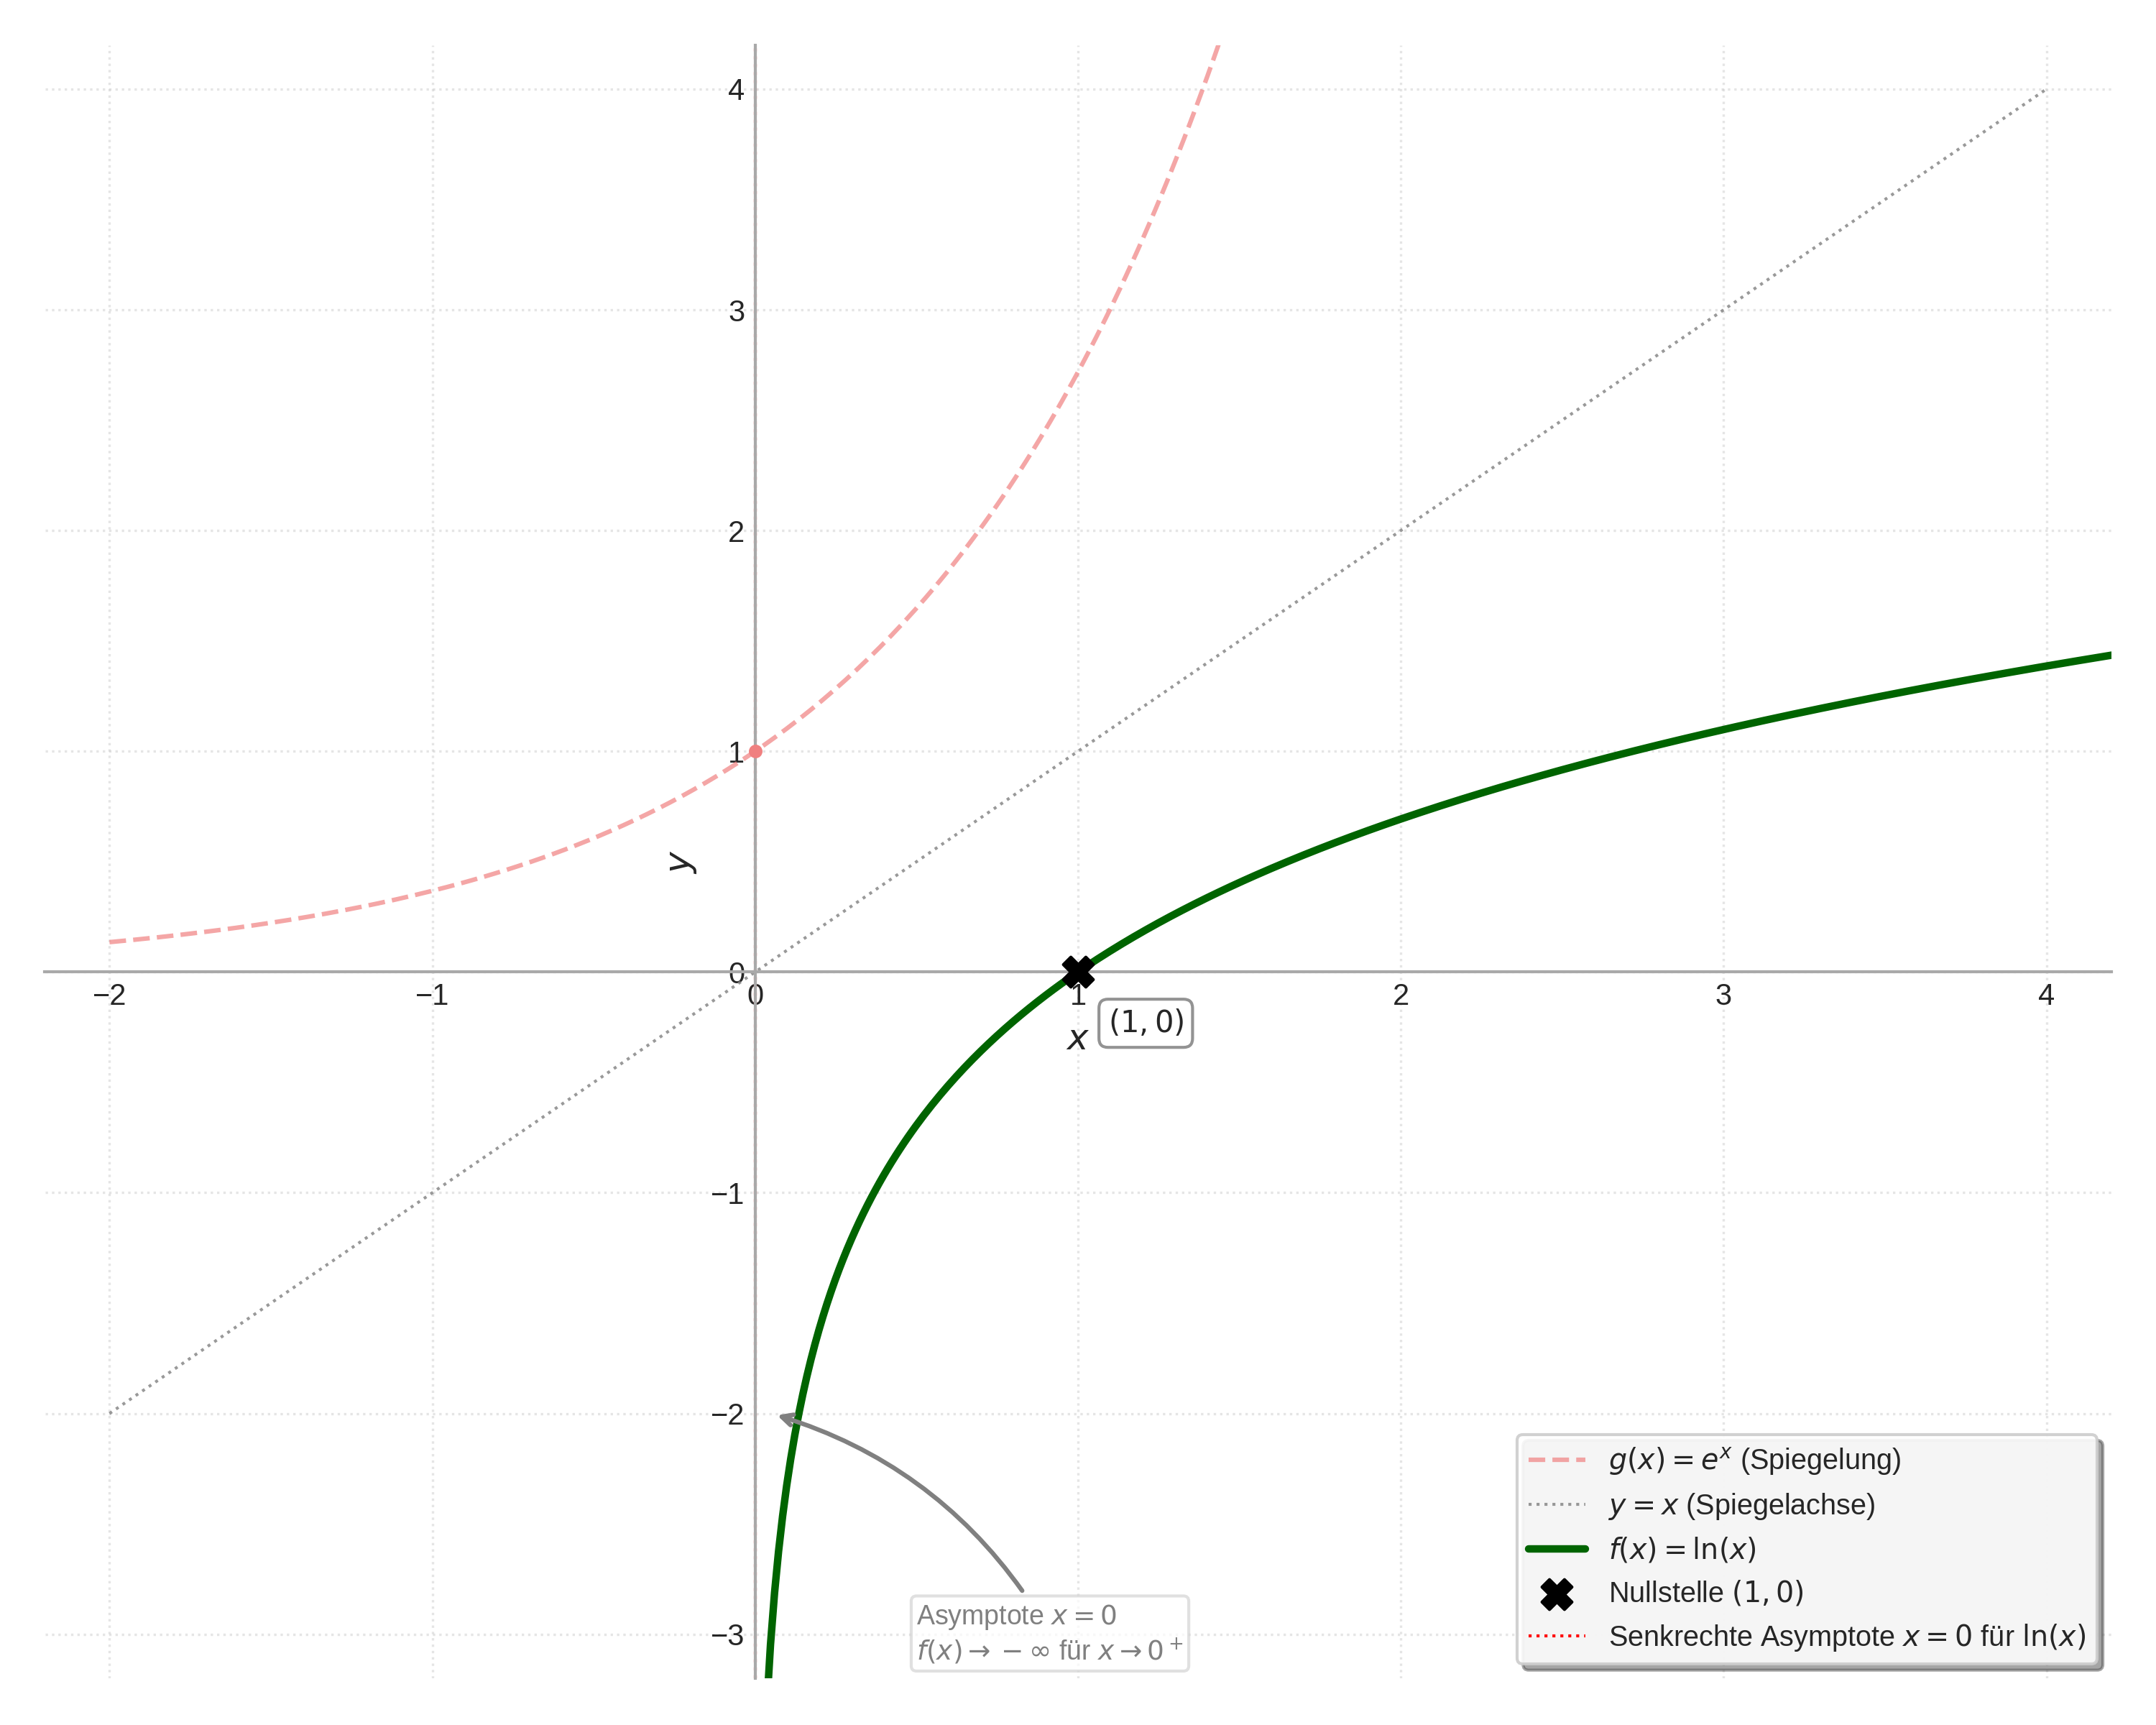
\includegraphics[width=0.8\textwidth]{grafiken/Logarithmusfunktion_lnx.png}
    \captionof{figure}{Graph der natürlichen Logarithmusfunktion \texorpdfstring{$f(x)=\ln(x)$}{f(x)=ln(x)}}
    \label{fig:log_funktion_lnx}
\end{center}
\textit{Selbst-Check:} Warum ist $\ln(1)=0$? Warum ist $\ln(e)=1$? (Antworten: Weil $e^0=1$ und $e^1=e$.)

\subsubsection{Wichtige Rechenregeln für Logarithmen (Logarithmengesetze)}
Für das Rechnen mit Logarithmen (egal zu welcher Basis) gibt es wichtige Gesetze, die sich aus den Potenzgesetzen ableiten lassen. Für den natürlichen Logarithmus lauten sie:

\begin{merksatzumgebung}[log_gesetze]{Logarithmengesetze für \texorpdfstring{$\ln(x)$}{ln(x)}}
Für $u, v > 0$ und $r \in \mathbb{R}$ gilt:
\begin{enumerate}[label=\arabic*)]
    \item \textbf{Produktregel:} $\ln(u \cdot v) = \ln(u) + \ln(v)$
    (Der Logarithmus eines Produkts ist die Summe der Logarithmen der Faktoren.)
    \item \textbf{Quotientenregel:} $\ln\left(\frac{u}{v}\right) = \ln(u) - \ln(v)$
    (Der Logarithmus eines Quotienten ist die Differenz der Logarithmen von Zähler und Nenner.)
    \item \textbf{Potenzregel:} $\ln(u^r) = r \cdot \ln(u)$
    (Der Logarithmus einer Potenz ist das Produkt aus dem Exponenten und dem Logarithmus der Basis.)
\end{enumerate}
Spezialfälle:
\begin{itemize}
    \item $\ln(e) = 1$
    \item $\ln(1) = 0$
    \item $\ln(e^x) = x$
    \item $e^{\ln(x)} = x$
\end{itemize}
\end{merksatzumgebung}

\begin{fehlerboxumgebung}{Logarithmengesetze richtig anwenden}
Die Logarithmengesetze sind mächtig, aber nur, wenn sie korrekt angewendet werden!
\begin{itemize}
    \item \textbf{Falsch:} $\ln(u+v) = \ln(u) + \ln(v)$. Der Logarithmus einer Summe ist NICHT die Summe der Logarithmen. Es gibt keine einfache Regel für $\ln(u+v)$.
    \item \textbf{Falsch:} $\ln(u-v) = \ln(u) - \ln(v)$. Analog zur Summe.
    \item \textbf{Falsch:} $\frac{\ln(u)}{\ln(v)} = \ln(u) - \ln(v)$ oder $\ln(\frac{u}{v})$. Die Division von Logarithmen ist NICHT dasselbe wie der Logarithmus eines Quotienten.
    \item \textbf{Falsch:} $(\ln(u))^r = r \ln(u)$. Die Potenzregel $\ln(u^r)=r\ln(u)$ gilt für den Logarithmus einer Potenz, nicht für eine Potenz des Logarithmus.
\end{itemize}
Überprüfe immer genau, ob du die Produkt-, Quotienten- oder Potenzregel korrekt anwendest!
\end{fehlerboxumgebung}

\begin{beispielumgebung}[anwendung_log_gesetze]{Anwendung der Logarithmengesetze}
\begin{enumerate}
    \item Vereinfache $\ln(2a) + \ln(3b) - \ln(6ab^2)$ für $a,b > 0$.
    $\ln(2a) + \ln(3b) - \ln(6ab^2) = \ln(2 \cdot a \cdot 3 \cdot b) - \ln(6ab^2)$ (Produktregel)
    $= \ln(6ab) - \ln(6ab^2)$
    $= \ln\left(\frac{6ab}{6ab^2}\right)$ (Quotientenregel)
    $= \ln\left(\frac{1}{b}\right) = \ln(b^{-1})$
    $= -1 \cdot \ln(b) = -\ln(b)$ (Potenzregel).

    \item Löse die Gleichung $e^{2x} = 5$ nach $x$.
    Wir wenden auf beiden Seiten den natürlichen Logarithmus an:
    $\ln(e^{2x}) = \ln(5)$
    Mit $\ln(e^A)=A$ folgt:
    $2x = \ln(5)$
    $x = \frac{\ln(5)}{2}$.
    Mit dem Taschenrechner: $\ln(5) \approx 1.609$, also $x \approx \frac{1.609}{2} \approx 0.8045$.
\end{enumerate}
\end{beispielumgebung}

\begin{aufgabenumgebung}{Rechnen mit Logarithmen}
\begin{enumerate}
    \item Vereinfache die folgenden Terme so weit wie möglich (alle Variablen seien positiv):
        \begin{itemize}
            \item $\ln(x^3) + \ln(x^2)$
            \item $\ln(a^5) - \ln(a^2)$
            \item $2\ln(u) - 3\ln(v)$
            \item $\frac{1}{2}\ln(16x^4)$
        \end{itemize}
    \item Löse die folgenden Exponentialgleichungen nach $x$. Gib das Ergebnis sowohl exakt als auch als Dezimalzahl (auf 3 Nachkommastellen gerundet) an.
        \begin{itemize}
            \item $e^x = 20$
            \item $2e^{3x} = 18$
            \item $e^{-0.5x+1} = 5$
            \item $100 \cdot (0.7)^x = 10$ (Tipp: Erst isolieren, dann logarithmieren. Du kannst hier $\ln$ verwenden, obwohl die Basis $0.7$ ist.)
        \end{itemize}
\end{enumerate}
\end{aufgabenumgebung}

\subsubsection{Ableitung und Stammfunktion des natürlichen Logarithmus}
\label{subsubsec:ableitung_stammfunktion_lnx}

Nachdem wir die grundlegenden Eigenschaften und Rechenregeln des natürlichen Logarithmus kennengelernt haben, wollen wir uns nun seiner Ableitung und seiner Rolle als Stammfunktion widmen.

\begin{merksatzumgebung}[ableitung_lnx]{Ableitung von \texorpdfstring{$f(x) = \ln(x)$}{f(x) = ln(x)}}
Die Ableitung der natürlichen Logarithmusfunktion $f(x) = \ln(x)$ für $x > 0$ ist:
\[ (\ln(x))' = \frac{1}{x} \]
\textit{Bemerkung:} Diese einfache und elegante Ableitung ist ein weiterer Grund, warum der natürliche Logarithmus in der Analysis so wichtig ist. Die Herleitung dieser Regel erfordert fortgeschrittenere Methoden (z.B. die Ableitung der Umkehrfunktion oder die Definition des Logarithmus über ein Integral), daher nehmen wir sie hier als gegeben hin.
\end{merksatzumgebung}

\begin{beispielumgebung}[anwendung_ableitung_lnx]{Ableitung von \texorpdfstring{$\ln(x)$}{ln(x)} anwenden}
\begin{enumerate}
    \item $f(x) = 5\ln(x) \implies f'(x) = 5 \cdot (\ln(x))' = 5 \cdot \frac{1}{x} = \frac{5}{x}$ (Faktorregel)
    \item $g(x) = x^2 + \ln(x) \implies g'(x) = (x^2)' + (\ln(x))' = 2x + \frac{1}{x}$ (Summenregel)
\end{enumerate}
\end{beispielumgebung}

Da die Ableitung von $\ln(x)$ gleich $\frac{1}{x}$ ist, ergibt sich direkt die Stammfunktion für $\frac{1}{x}$.

\begin{merksatzumgebung}[stammfunktion_1durchx]{Stammfunktion von \texorpdfstring{$f(x) = \frac{1}{x}$}{f(x) = 1/x}}
Die Menge aller Stammfunktionen (das unbestimmte Integral) von $f(x) = \frac{1}{x}$ ist:
\[ \int \frac{1}{x} \,dx = \ln|x| + C \]
\textbf{Wichtig:} Da der Logarithmus nur für positive Zahlen definiert ist, der Term $\frac{1}{x}$ aber auch für negative $x$ existiert, schreiben wir $\ln|x|$ (Logarithmus des Betrags von $x$), um den Definitionsbereich der Stammfunktion ($x \neq 0$) abzudecken.
\begin{itemize}
    \item Für $x > 0$ ist $|x|=x$, also $\int \frac{1}{x} \,dx = \ln(x) + C$.
    \item Für $x < 0$ ist $|x|=-x$. Die Ableitung von $\ln(-x)$ ist nach der Kettenregel $\frac{1}{-x} \cdot (-1) = \frac{1}{x}$. Also ist auch hier $\ln(-x)+C$ eine Stammfunktion.
\end{itemize}
Die Schreibweise $\ln|x|+C$ fasst beide Fälle zusammen.
\end{merksatzumgebung}

\begin{beispielumgebung}[integration_kdurchx]{Integrieren von \texorpdfstring{$\frac{k}{x}$}{k/x}}
Bestimme $\int \frac{7}{x} \,dx$.
\[ \int \frac{7}{x} \,dx = 7 \int \frac{1}{x} \,dx = 7 \ln|x| + C \]
\end{beispielumgebung}

\begin{fehlerboxumgebung}{Stammfunktion von $1/x$ – Den Betrag nicht vergessen!}
Die Stammfunktion von $f(x)=\frac{1}{x}$ ist $F(x)=\ln|x|+C$. Warum der Betrag?
\begin{itemize}
    \item Die Funktion $f(x)=\frac{1}{x}$ ist für alle $x \neq 0$ definiert (also für positive und negative $x$).
    \item Die Funktion $\ln(x)$ ist aber nur für $x>0$ definiert.
    \item Für $x<0$ ist die Funktion $\ln(-x)$ definiert, und ihre Ableitung ist $\frac{1}{-x} \cdot (-1) = \frac{1}{x}$.
    \item $\ln|x|$ fasst beide Fälle ($\ln(x)$ für $x>0$ und $\ln(-x)$ für $x<0$) korrekt zusammen.
\end{itemize}
Bei bestimmten Integralen über Intervalle, die nur positive oder nur negative $x$-Werte enthalten, kannst du den Betrag entsprechend auflösen. Bei unbestimmten Integralen ist $\ln|x|+C$ die präziseste Angabe.
\end{fehlerboxumgebung}

\begin{aufgabenumgebung}{Ableiten und Integrieren mit \texorpdfstring{$\ln(x)$}{ln(x)}}
\begin{enumerate}
    \item Bilde die erste Ableitung der folgenden Funktionen:
        \begin{itemize}
            \item $f_1(x) = -2\ln(x) + e^x$
            \item $f_2(x) = x^3 \ln(x)$ (Produktregel!)
            \item $f_3(x) = \frac{\ln(x)}{x}$ (Quotientenregel!)
        \end{itemize}
    \item Bestimme die Menge aller Stammfunktionen:
        \begin{itemize}
            \item $g_1(x) = \frac{3}{x} - 2x + 1$
            \item $g_2(x) = \frac{x^2+x-1}{x}$ (Tipp: Den Bruch zuerst aufteilen!)
        \end{itemize}
\end{enumerate}
\end{aufgabenumgebung}

\subsubsection{Ableitung von verketteten Logarithmusfunktionen: \texorpdfstring{$f(x) = \ln(h(x))$}{f(x) = ln(h(x))}}
Sehr oft tritt der Logarithmus als äußere Funktion einer Verkettung auf. Hier benötigen wir die Kettenregel: $(g(h(x)))' = g'(h(x)) \cdot h'(x)$.

Wenn $f(x) = \ln(h(x))$, dann ist:
\begin{itemize}
    \item Äußere Funktion: $g(u) = \ln(u) \implies g'(u) = \frac{1}{u}$.
    \item Innere Funktion: $h(x)$. Ihre Ableitung ist $h'(x)$.
\end{itemize}
Somit ist die Ableitung von $f(x) = \ln(h(x))$:
\[ (\ln(h(x)))' = \frac{1}{h(x)} \cdot h'(x) = \frac{h'(x)}{h(x)} \]

\begin{merksatzumgebung}[ableitung_lnhx]{Ableitung von \texorpdfstring{$\ln(h(x))$}{ln(h(x))} (Spezialfall der Kettenregel)}
Für eine differenzierbare Funktion $h(x)$ mit $h(x)>0$ gilt:
\[ (\ln(h(x)))' = \frac{h'(x)}{h(x)} \]
'Ableitung der inneren Funktion geteilt durch die innere Funktion.'
\end{merksatzumgebung}

\begin{fehlerboxumgebung}{Ableitung von $\ln(h(x))$ – Die Kettenregel beachten!}
Die Formel $(\ln(h(x)))' = \frac{h'(x)}{h(x)}$ ist eine direkte Anwendung der Kettenregel. Häufige Fehler sind:
\begin{itemize}
    \item \textbf{Innere Ableitung $h'(x)$ im Zähler vergessen:} Man schreibt nur $\frac{1}{h(x)}$.
    \item \textbf{Kehrwert falsch gebildet:} Man schreibt $h(x) \cdot h'(x)$ oder Ähnliches.
    \item \textbf{Definitionsbereich von $\ln(h(x))$ nicht beachtet:} Die Ableitung existiert nur dort, wo $h(x)>0$ ist und $h(x)$ differenzierbar ist.
\end{itemize}
Identifiziere immer klar die innere Funktion $h(x)$ und bilde ihre Ableitung $h'(x)$ korrekt.
\end{fehlerboxumgebung}

\begin{beispielumgebung}[kettenregel_lnhx]{Kettenregel mit \texorpdfstring{$\ln(h(x))$}{ln(h(x))}}
\begin{enumerate}
    \item $f(x) = \ln(x^2+1)$. (Hier ist $x^2+1$ immer positiv, also $D_f=\mathbb{R}$)
        Innere Funktion: $h(x) = x^2+1 \implies h'(x) = 2x$.
        $f'(x) = \frac{2x}{x^2+1}$.

    \item $g(x) = \ln(3x-5)$. (Definiert für $3x-5 > 0 \implies 3x > 5 \implies x > 5/3$)
        Innere Funktion: $h(x) = 3x-5 \implies h'(x) = 3$.
        $g'(x) = \frac{3}{3x-5}$.

    \item $k(x) = ( \ln(x) )^3$. (Definiert für $x>0$)
        Hier ist die \textbf{äußere Funktion} $g(u)=u^3$ und die \textbf{innere Funktion} $h(x)=\ln(x)$.
        $g'(u) = 3u^2$.
        $h'(x) = \frac{1}{x}$.
        $k'(x) = g'(h(x)) \cdot h'(x) = 3(\ln(x))^2 \cdot \frac{1}{x} = \frac{3(\ln x)^2}{x}$.
\end{enumerate}
\end{beispielumgebung}

\begin{aufgabenumgebung}{Kettenregel mit \texorpdfstring{$\ln(h(x))$}{ln(h(x))} üben}
Bilde die erste Ableitung der folgenden Funktionen. Gib auch den maximalen Definitionsbereich an.
\begin{enumerate}
    \item $f_1(x) = \ln(5x)$
    \item $f_2(x) = \ln(x^3+x)$ (für $x>0$)
    \item $f_3(x) = x \cdot \ln(2x+1)$ (Produkt- und Kettenregel!)
    \item $f_4(x) = e^{\ln(x^2)}$ (Tipp: Vereinfache zuerst mit den Logarithmus-/Exponentialgesetzen! Was ist $e^{\ln A}$?)
\end{enumerate}
\end{aufgabenumgebung}

\subsection{Kurvendiskussion von Funktionen mit \texorpdfstring{$\ln(x)$}{ln(x)}}
\label{subsec:kurvendiskussion_lnx}

Funktionen, die den natürlichen Logarithmus enthalten (oft in Kombination mit Polynomen), können interessante Verläufe aufweisen. Die Schritte der Kurvendiskussion bleiben dieselben, aber wir müssen die speziellen Eigenschaften des Logarithmus (Definitionsbereich, Grenzwerte) beachten.

\begin{infoboxumgebung}{Wichtige Grenzwerte mit \texorpdfstring{$\ln(x)$}{ln(x)}}
Für das Verhalten von Funktionen mit $\ln(x)$ im Unendlichen sind folgende Grenzwerte oft nützlich:
\begin{itemize}
    \item $\lim_{x \to \infty} \frac{\ln(x)}{x^n} = 0$ für jedes $n > 0$. (Jede noch so kleine positive Potenz von $x$ wächst schneller als $\ln(x)$.)
    \item $\lim_{x \to 0^+} x^n \ln(x) = 0$ für jedes $n > 0$. (Für $x \to 0^+$ geht $\ln(x) \to -\infty$, aber $x^n$ geht 'schneller' gegen $0$.)
\end{itemize}
Diese Regeln helfen zu verstehen, welcher Teil einer Funktion (z.B. in einem Produkt $x \cdot \ln x$) das Verhalten für $x \to \infty$ oder $x \to 0^+$ dominiert.
\end{infoboxumgebung}

\begin{beispielumgebung}[beispiel_kurvendisk_xlnx]{Kurvendiskussion mit \texorpdfstring{$\ln x$}{ln(x)} – Untersuchung von \texorpdfstring{$f(x) = x \ln(x)$}{f(x) = x ln(x)}}
\begin{enumerate}
    \item \textbf{Definitionsbereich:} Wegen $\ln(x)$ muss $x>0$ sein. Also $D_f = (0, \infty) = \mathbb{R}^+$.
    \item \textbf{Symmetrie:} Da $D_f$ nicht symmetrisch zum Ursprung ist, kann keine einfache Symmetrie vorliegen.
    \item \textbf{Verhalten an den Rändern des Definitionsbereichs:}
        \begin{itemize}
            \item Für $x \to \infty$: $x \to \infty$ und $\ln(x) \to \infty$. Also $\lim_{x \to \infty} x \ln(x) = +\infty$.
            \item Für $x \to 0^+$: $x \to 0$ und $\ln(x) \to -\infty$. Wir haben einen Typ '$0 \cdot (-\infty)$'.
            Mit dem oben genannten Grenzwert $\lim_{x \to 0^+} x^n \ln(x) = 0$ (hier für $n=1$) gilt:
            $\lim_{x \to 0^+} x \ln(x) = 0$.
            Der Graph nähert sich also dem Ursprung $(0|0)$ für $x \to 0^+$.
        \end{itemize}
    \item \textbf{y-Achsenabschnitt:} Gibt es nicht, da $x=0$ nicht im Definitionsbereich ist.
    \item \textbf{Nullstellen:} $f(x)=0 \implies x \ln(x) = 0$.
        Da $x>0$ im Definitionsbereich, kann $x$ nicht Null sein. Also muss $\ln(x)=0$ sein.
        $\ln(x)=0 \implies x = e^0 = 1$.
        Einzige Nullstelle bei $N(1|0)$.
    \item \textbf{Erste Ableitung $f'(x)$:} Mit Produktregel $u(x)=x, u'(x)=1, v(x)=\ln(x), v'(x)=1/x$.
        $f'(x) = 1 \cdot \ln(x) + x \cdot \frac{1}{x} = \ln(x) + 1$.
    \item \textbf{Extremstellen:} $f'(x)=0 \implies \ln(x) + 1 = 0 \implies \ln(x) = -1$.
        $x_E = e^{-1} = \frac{1}{e} \approx 0.368$.
    \item \textbf{Zweite Ableitung $f''(x)$:} $f''(x) = (\ln(x)+1)' = \frac{1}{x} + 0 = \frac{1}{x}$.
    \item \textbf{Art der Extremstelle bei $x_E=1/e$ mit $f''$ prüfen:}
        $f''(1/e) = \frac{1}{1/e} = e$.
        Da $f'(1/e)=0$ und $f''(1/e)=e > 0 \implies$ Lokaler Tiefpunkt bei $x_E=1/e$.
        $y_T = f(1/e) = \frac{1}{e} \ln(\frac{1}{e}) = \frac{1}{e} \ln(e^{-1}) = \frac{1}{e} \cdot (-1) = -\frac{1}{e} \approx -0.368$.
        Tiefpunkt $T(1/e | -1/e)$.
    \item \textbf{Monotonie:} Nullstelle von $f'(x)=\ln(x)+1$ ist $x=1/e$.
        \begin{itemize}
            \item $0 < x < 1/e$ (z.B. $x=0.1 \approx 1/(2e)$): $\ln(0.1) \approx -2.3$. $f'(0.1) = -2.3+1 = -1.3 < 0 \implies$ fallend.
            \item $x > 1/e$ (z.B. $x=1$): $f'(1) = \ln(1)+1 = 0+1 = 1 > 0 \implies$ steigend.
        \end{itemize}
        Fallend für $x \in (0, 1/e]$, steigend für $x \in [1/e, \infty)$.
    \item \textbf{Wendepunkte:} $f''(x_W)=0 \implies \frac{1}{x_W}=0$. Diese Gleichung hat keine Lösung, da ein Bruch nur Null ist, wenn der Zähler Null ist (hier ist der Zähler 1). Also keine Nullstellen von $f''(x)$.
    \item \textbf{Krümmungsverhalten:} Da $D_f=(0,\infty)$, ist $x$ immer positiv. Somit ist $f''(x)=\frac{1}{x}$ immer positiv für alle $x \in D_f$.
        Der Graph ist also im gesamten Definitionsbereich linksgekrümmt (konvex). Es gibt keine Wendepunkte.
    \item \textbf{Skizze:}
        \begin{center}
            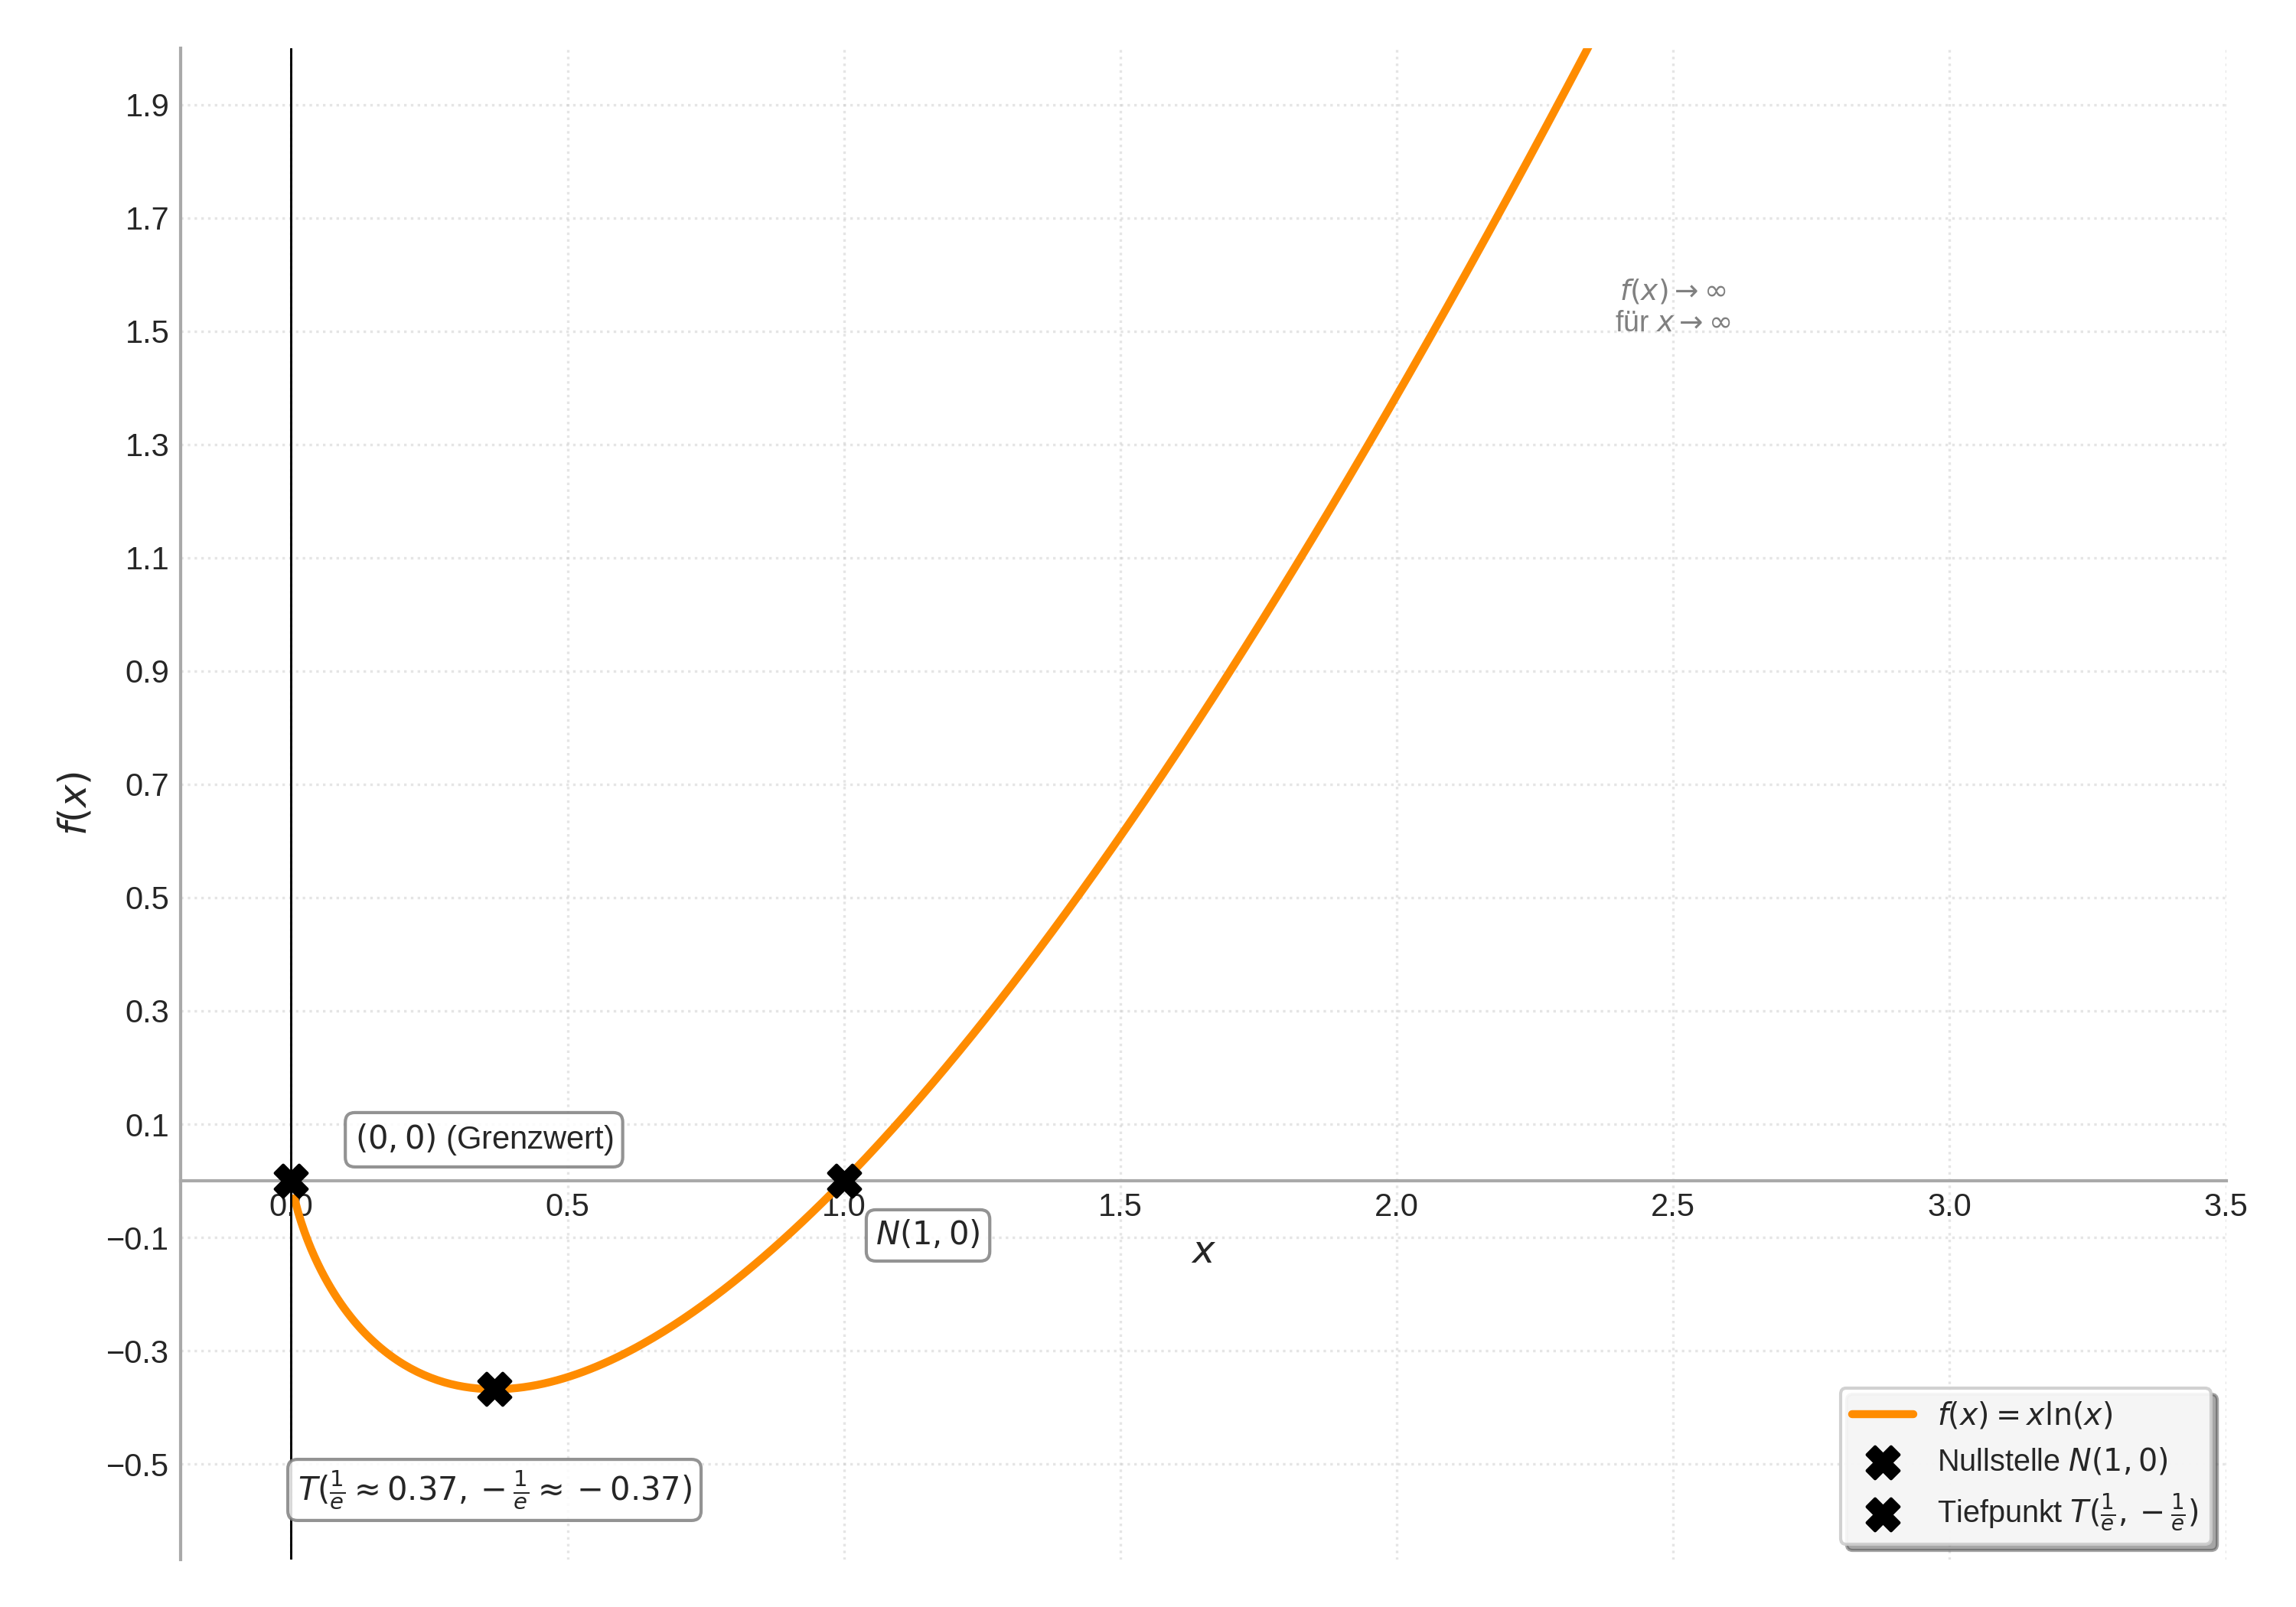
\includegraphics[width=0.9\textwidth]{grafiken/Kurvendiskussion_xlnx.png}
            \captionof{figure}{Graph von \texorpdfstring{$f(x)=x\ln(x)$}{f(x)=xln(x)}}
            \label{fig:kurvendisk_xlnx}
        \end{center}
\end{enumerate}
\end{beispielumgebung}

\begin{aufgabenumgebung}{Kurvendiskussionen mit Logarithmusfunktionen}
Führe eine vollständige Kurvendiskussion für die folgenden Funktionen durch.
\begin{enumerate}
    \item $f(x) = \ln(x^2+2)$ (Beachte den Definitionsbereich!)
    \item $g(x) = \frac{\ln x}{x}$ (für $x>0$)
    \item \textbf{Für Experten:} $h(x) = x^2 \ln(x)$ (für $x>0$)
\end{enumerate}
\end{aufgabenumgebung}

\begin{tippumgebung}{Anwendungen von Logarithmusfunktionen}
Logarithmusfunktionen sind oft die 'Antwort', wenn es um die Umkehrung exponentieller Prozesse geht oder wenn Größen über viele Zehnerpotenzen variieren.
\begin{itemize}
    \item \textbf{Halbwertszeiten/Verdopplungszeiten:} Berechnung der Zeit, bis sich eine Menge halbiert oder verdoppelt (siehe Aufgabe zum radioaktiven Zerfall im Exponentialfunktionskapitel).
    \item \textbf{Skalen:} pH-Wert (misst Säuregrad), Dezibel (Lautstärke), Richterskala (Erdbebenstärke) sind logarithmische Skalen. Eine Erhöhung um 1 auf der Skala bedeutet oft eine Verzehnfachung der eigentlichen physikalischen Größe.
    \item \textbf{Wachstumsmodelle:} Manchmal ist es einfacher, das logarithmierte Wachstum zu analysieren.
\end{itemize}
\end{tippumgebung}

\subsubsection{Integration mit Logarithmusfunktionen – Partielle Integration und ein wichtiger Spezialfall der Substitution}
\label{subsubsec:integration_lnx_neu}

Wir wissen bereits, dass die Stammfunktion von $f(x)=\frac{1}{x}$ die Funktion $F(x)=\ln|x|+C$ ist. Aber wie integriert man die Logarithmusfunktion $\ln(x)$ selbst? Und gibt es spezielle Strukturen bei Integralen, die auf Logarithmen führen?

\textbf{1. Die Stammfunktion von $\ln(x)$ – Ein Fall für die partielle Integration}

Um $\int \ln(x) \,dx$ zu berechnen, verwenden wir einen kleinen Trick und die partielle Integration.
Erinnerung Partielle Integration: $\int u'(x)v(x) \,dx = u(x)v(x) - \int u(x)v'(x) \,dx$.

Wir schreiben $\ln(x)$ als Produkt: $\ln(x) = 1 \cdot \ln(x)$.
Nun wählen wir geschickt:
\begin{itemize}
    \item $u'(x) = 1 \implies u(x) = \int 1 \,dx = x$
    \item $v(x) = \ln(x) \implies v'(x) = \frac{1}{x}$
\end{itemize}
Einsetzen in die Formel der partiellen Integration:
\begin{align*} \int \underbrace{1}_{u'(x)} \cdot \underbrace{\ln(x)}_{v(x)} \,dx &= \underbrace{x}_{u(x)} \cdot \underbrace{\ln(x)}_{v(x)} - \int \underbrace{x}_{u(x)} \cdot \underbrace{\frac{1}{x}}_{v'(x)} \,dx \\ &= x \ln(x) - \int 1 \,dx \\ &= x \ln(x) - x + C \end{align*}

\begin{merksatzumgebung}[stammfunktion_lnx]{Stammfunktion von $\ln(x)$}
Die Menge aller Stammfunktionen (das unbestimmte Integral) von $f(x) = \ln(x)$ für $x>0$ ist:
\[ \int \ln(x) \,dx = x \ln(x) - x + C \]
Oder ausgeklammert: $\int \ln(x) \,dx = x(\ln(x) - 1) + C$.
Diese wichtige Stammfunktion solltest du dir merken!
\end{merksatzumgebung}

\begin{beispielumgebung}[best_integral_lnx]{Bestimmtes Integral von \texorpdfstring{$\ln(x)$}{ln(x)}}
Berechne $\int_1^e \ln(x) \,dx$.
Wir verwenden die Stammfunktion $F(x) = x\ln(x) - x$:
\begin{align*} \int_1^e \ln(x) \,dx &= [x\ln(x) - x]_1^e \\ &= (e \cdot \ln(e) - e) - (1 \cdot \ln(1) - 1) \\ &= (e \cdot 1 - e) - (1 \cdot 0 - 1) && \text{(da } \ln(e)=1 \text{ und } \ln(1)=0) \\ &= (e - e) - (0 - 1) \\ &= 0 - (-1) = 1 \end{align*}
Der Flächeninhalt unter dem Graphen von $\ln(x)$ zwischen $x=1$ und $x=e$ beträgt also genau 1.
\begin{center}
    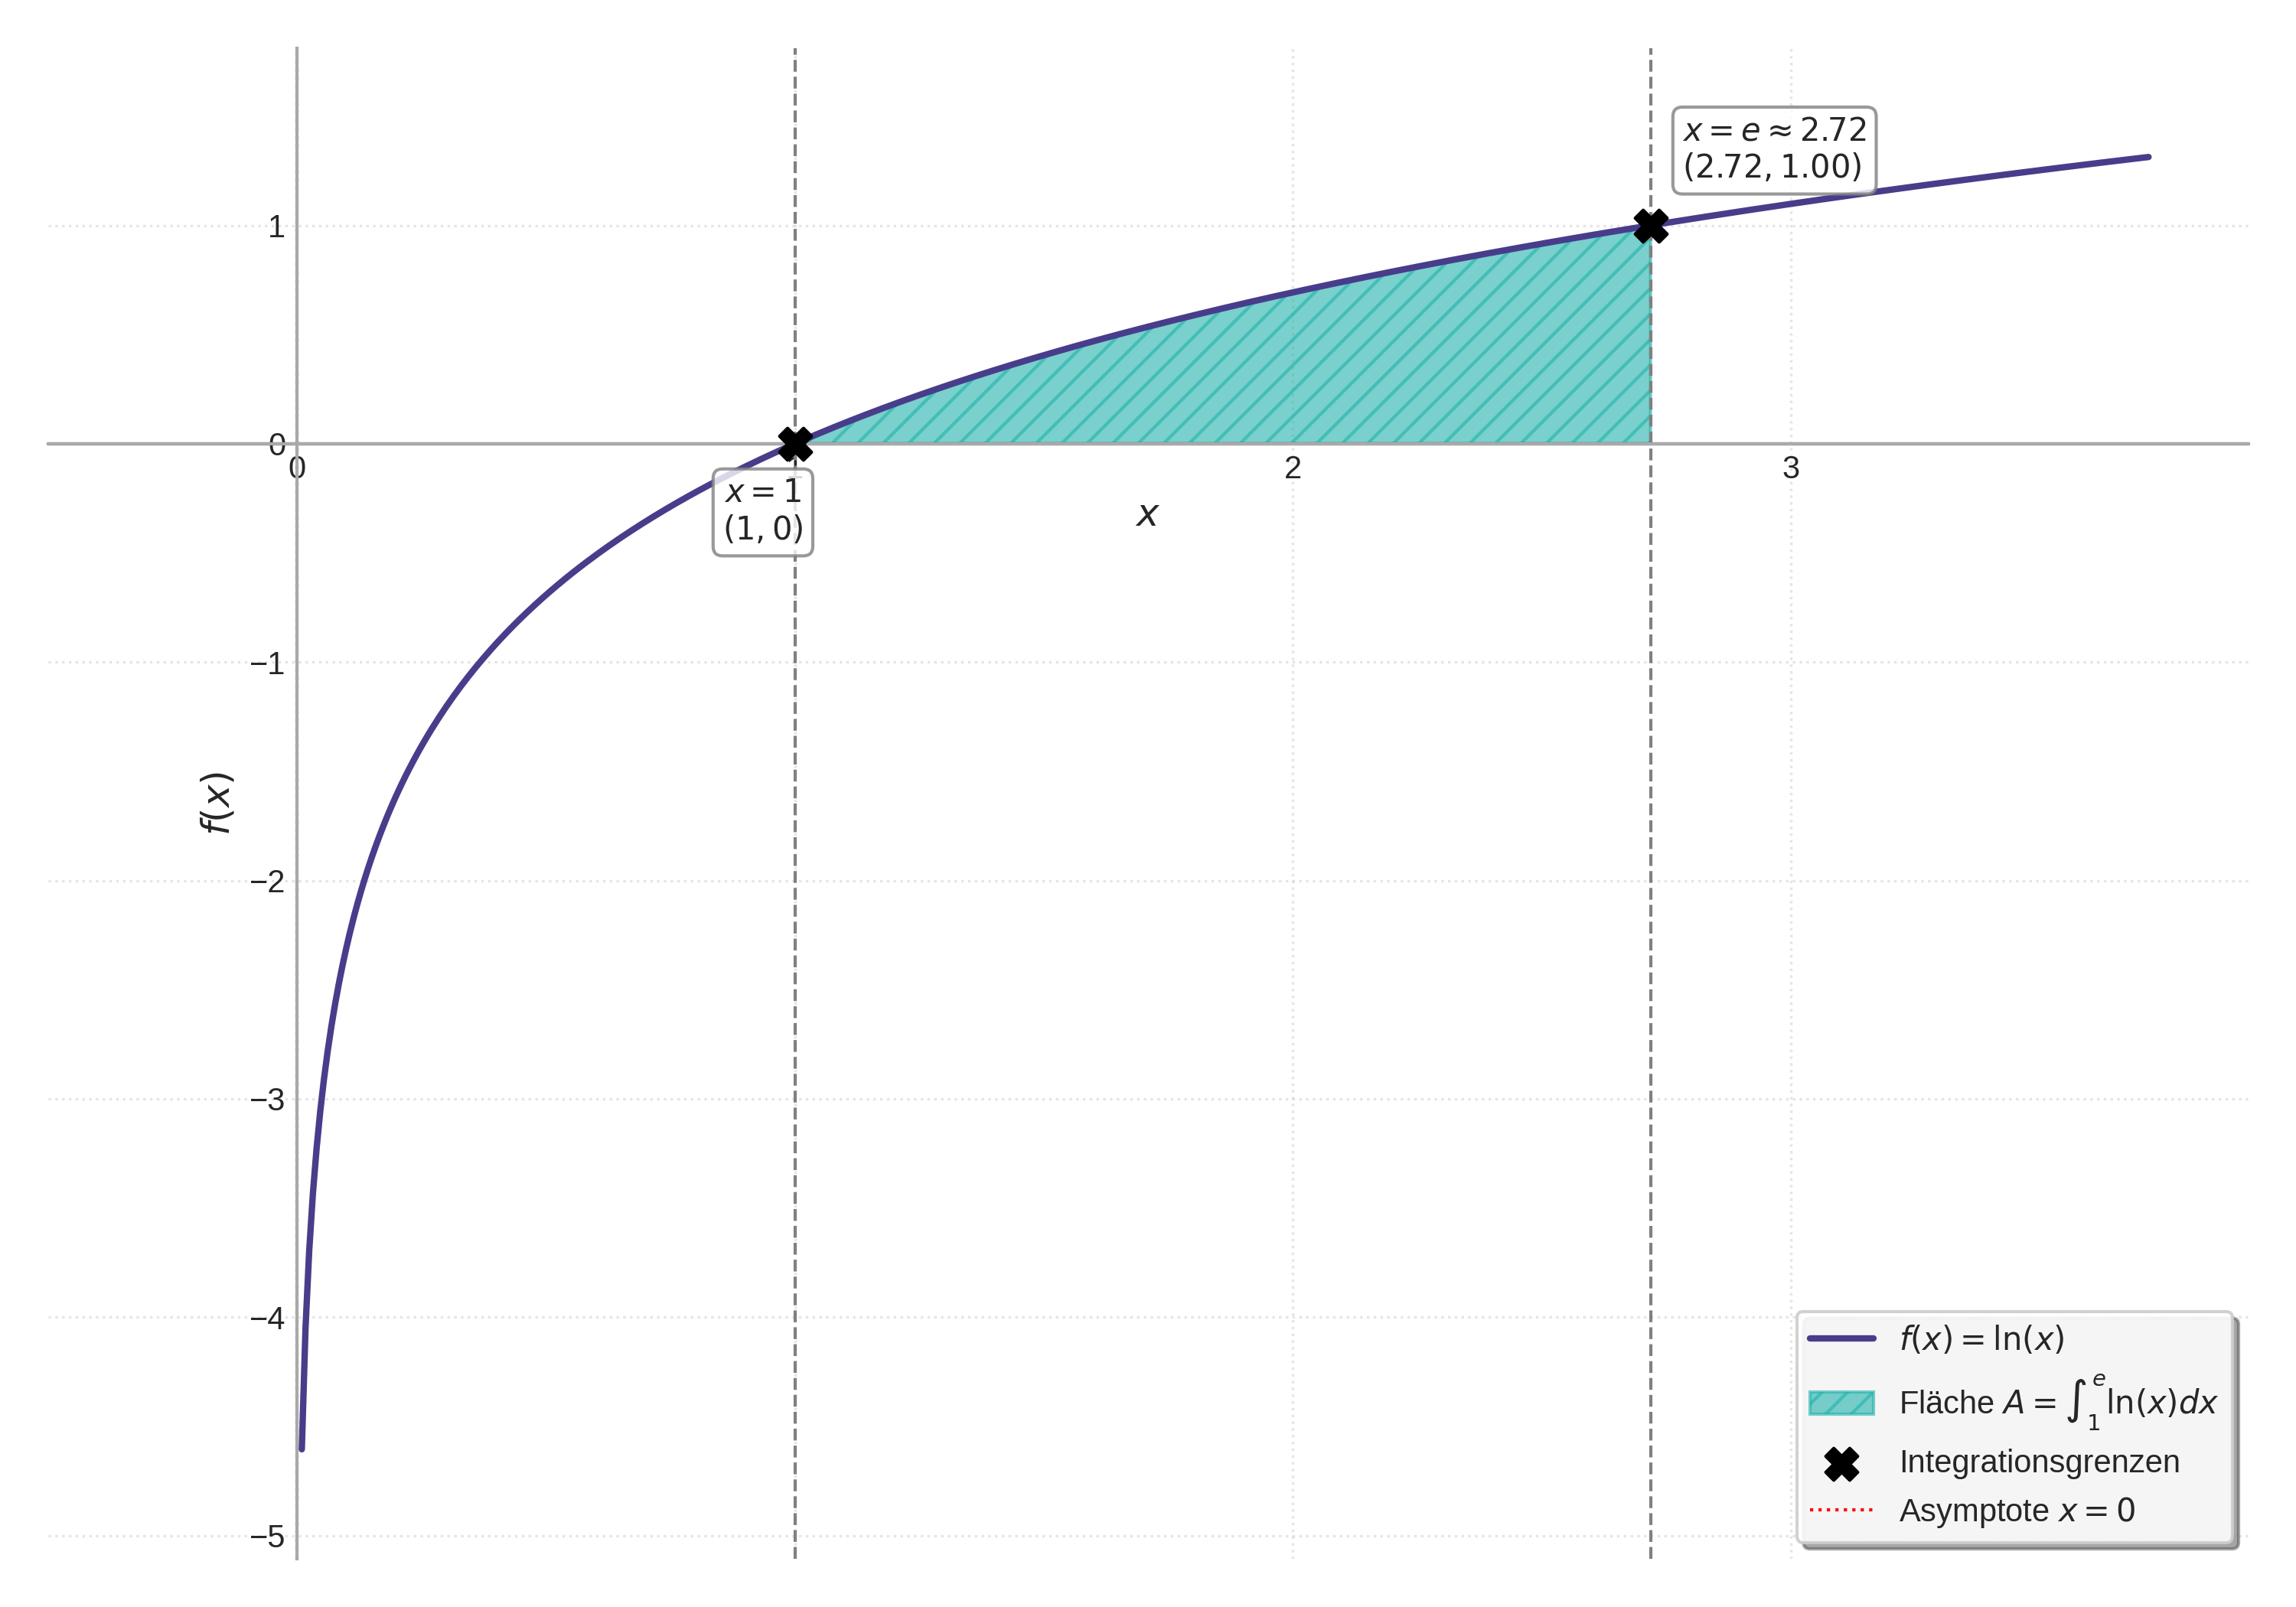
\includegraphics[width=0.8\textwidth]{grafiken/Integral_Flaeche_lnx.png}
    \captionof{figure}{Fläche unter \texorpdfstring{$f(x)=\ln(x)$}{f(x)=ln(x)} von $x=1$ bis $x=e$}
    \label{fig:flaeche_lnx}
\end{center}
\end{beispielumgebung}

\textbf{2. Ein wichtiger Spezialfall der Substitution: $\int \frac{g'(x)}{g(x)} \,dx$}

Betrachten wir Integrale, bei denen der Zähler die Ableitung des Nenners ist (oder ein Vielfaches davon).
Also Integrale der Form $\int \frac{g'(x)}{g(x)} \,dx$.

Hier hilft die Substitution $u = g(x)$.
Dann ist $\frac{du}{dx} = g'(x)$, also $du = g'(x)dx$.
Setzen wir das ins Integral ein:
\[ \int \frac{g'(x)}{g(x)} \,dx = \int \frac{1}{g(x)} \cdot g'(x)dx = \int \frac{1}{u} \,du \]
Das Integral von $\frac{1}{u}$ ist $\ln|u|+C$.
Rücksubstituieren wir $u=g(x)$, erhalten wir:

\begin{merksatzumgebung}[integration_gstrich_durch_g]{Integration von $\frac{\text{Ableitung}}{\text{Funktion}}$}
Für eine differenzierbare Funktion $g(x)$ mit $g(x) \neq 0$ gilt:
\[ \int \frac{g'(x)}{g(x)} \,dx = \ln|g(x)| + C \]
Diese Regel ist sehr nützlich und erspart oft die explizite Durchführung der Substitution.
\end{merksatzumgebung}

\begin{beispielumgebung}[anwendung_int_gstrich_g]{Anwendung der Regel \texorpdfstring{$\int \frac{g'(x)}{g(x)} \,dx$}{Integral g'(x)/g(x) dx}}
\begin{enumerate}
    \item \textbf{Integral $\int \frac{2x}{x^2+1} \,dx$}
        Sei $g(x) = x^2+1$. Dann ist $g'(x) = 2x$.
        Der Integrand hat genau die Form $\frac{g'(x)}{g(x)}$.
        Also: $\int \frac{2x}{x^2+1} \,dx = \ln|x^2+1| + C$.
        Da $x^2+1$ immer positiv ist, können wir die Betragsstriche weglassen: $\ln(x^2+1) + C$.

    \item \textbf{Integral $\int \frac{x}{x^2-4} \,dx$}
        Sei $g(x) = x^2-4$. Dann ist $g'(x) = 2x$.
        Im Zähler steht $x$, wir bräuchten aber $2x$. Wir können den Integranden mit $\frac{2}{2}$ erweitern:
        $\int \frac{x}{x^2-4} \,dx = \int \frac{1}{2} \cdot \frac{2x}{x^2-4} \,dx = \frac{1}{2} \int \frac{2x}{x^2-4} \,dx$.
        Jetzt hat der Bruch die Form $\frac{g'(x)}{g(x)}$.
        Also: $\frac{1}{2} \ln|x^2-4| + C$.
\end{enumerate}
\end{beispielumgebung}

\begin{aufgabenumgebung}{Integration mit Logarithmusfunktionen üben}
\begin{enumerate}
    \item Berechne die folgenden unbestimmten Integrale:
        \begin{itemize}
            \item $\int (3\ln(x) - 2x) \,dx$
            \item $\int \frac{5x^4}{x^5+1} \,dx$
            \item $\int \frac{e^x}{e^x+3} \,dx$
            \item $\int \frac{1}{2x+7} \,dx$ (Tipp: Erweitere so, dass der Zähler die Ableitung des Nenners ist.)
        \end{itemize}
    \item \textbf{Flächenberechnung:}
        Die Funktion $f(x) = \frac{1}{x}$ ist im ersten Quadranten gegeben.
        \begin{itemize}
            \item Berechne den Inhalt der Fläche, die der Graph von $f(x)$ mit der x-Achse im Intervall $[1, e]$ einschließt.
            \item Berechne den Inhalt der Fläche, die der Graph von $f(x)$ mit der x-Achse im Intervall $[1, b]$ für ein beliebiges $b>1$ einschließt. Was passiert mit dieser Fläche, wenn $b \to \infty$? (Uneigentliches Integral)
        \end{itemize}
    \item \textbf{Anwendung partielle Integration (anspruchsvoller):}
        Berechne $\int x^2 \ln(x) \,dx$. (Tipp: Wähle $v(x)=\ln(x)$ und $u'(x)=x^2$).
\end{enumerate}
\end{aufgabenumgebung}

\begin{kurzknappumgebung}{Logarithmusfunktionen – Analysis im Überblick}
\begin{itemize}
    \item \textbf{Natürlicher Logarithmus $\ln(x)$:} Umkehrfunktion von $e^x$. $D_f=(0,\infty)$, $W_f=\mathbb{R}$. Nullstelle bei $x=1$. Senkrechte Asymptote $x=0$.
    \item \textbf{Logarithmengesetze:} Helfen beim Umformen von Termen mit Logarithmen.
    \item \textbf{Ableitung:} $(\ln x)' = \frac{1}{x}$. Für verkettete Funktionen: $(\ln(h(x)))' = \frac{h'(x)}{h(x)}$.
    \item \textbf{Stammfunktion:} $\int \frac{1}{x} \,dx = \ln|x|+C$. $\int \ln(x) \,dx = x\ln(x) - x + C$.
    \item \textbf{Wichtiger Spezialfall der Substitution:} $\int \frac{g'(x)}{g(x)} \,dx = \ln|g(x)|+C$.
    \item \textbf{Kurvendiskussion:} Beachte Definitionsbereich und Grenzwerte an den Rändern.
\end{itemize}
\end{kurzknappumgebung}

\begin{infoboxumgebung}{Ausblick: Die Reise geht weiter – Trigonometrische Funktionen}
Mit den Exponential- und Logarithmusfunktionen hast du zwei sehr wichtige nicht-polynomielle Funktionsklassen kennengelernt, die in unzähligen Bereichen der Wissenschaft und des Alltags Anwendung finden.

Als Nächstes auf unserer mathematischen Entdeckungsreise stehen die \textbf{trigonometrischen Funktionen} ($\sin x, \cos x, \tan x$) auf dem Programm. Diese periodischen Funktionen sind unerlässlich, um Schwingungen, Wellen und zyklische Vorgänge zu beschreiben – von den Gezeiten über Schallwellen bis hin zu den Bewegungen von Planeten.

Auch für diese neuen Funktionstypen werden wir lernen, wie man sie ableitet und integriert, und wie wir sie in Kurvendiskussionen und Anwendungsaufgaben nutzen können. Die Werkzeuge der Differential- und Integralrechnung, die du bisher erworben hast, werden dabei immer wieder von zentraler Bedeutung sein. Die Mathematik baut aufeinander auf – und das ist das Schöne daran!
\end{infoboxumgebung}

\begin{aufgabenumgebung}{Checkliste: Das Wesen des Logarithmus und der $\ln$-Funktion verstehen}
Der Logarithmus, insbesondere der natürliche Logarithmus $\ln(x)$, ist ein Schlüsselkonzept mit vielen Facetten. Diese Fragen helfen dir, die Grundlagen zu festigen:

\begin{enumerate}[label=(\alph*)]
    \item \textbf{Definition und Umkehrbeziehung:}
    \begin{itemize}
        \item Erkläre mit eigenen Worten, was $\log_b(y)=x$ bedeutet. Was ist die spezielle Basis beim natürlichen Logarithmus $\ln(x)$?
        \item Warum muss gelten: $e^{\ln(x)} = x$ (für $x>0$) und $\ln(e^x) = x$ (für alle $x \in \mathbb{R}$)? Erläutere dies am Konzept der Umkehrfunktion.
        \item Begründe, warum $\ln(1)=0$ und $\ln(e)=1$ sein muss.
    \end{itemize}
    \item \textbf{Definitionsbereich und Graph:}
    \begin{itemize}
        \item Warum ist der Definitionsbereich der Funktion $f(x)=\ln(x)$ auf positive reelle Zahlen ($x>0$) beschränkt? Wie hängt das mit dem Wertebereich der $e$-Funktion zusammen?
        \item Beschreibe die wesentlichen Unterschiede im Graphenverlauf zwischen $g(x)=e^x$ und $f(x)=\ln(x)$ bezüglich Monotonie, Krümmung und Asymptoten. Wie kommt die geometrische Beziehung (Spiegelung an $y=x$) zustande?
    \end{itemize}
    \item \textbf{Logarithmengesetze anwenden und verstehen:}
    \begin{itemize}
        \item Die Regel $\ln(u^r) = r \cdot \ln(u)$ ist besonders nützlich beim Lösen von Exponentialgleichungen. Erkläre, warum diese Regel das 'Herunterholen' des Exponenten ermöglicht.
        \item Ist die Aussage $\ln(a+b) = \ln(a) + \ln(b)$ korrekt? Überprüfe mit einem Zahlenbeispiel und vergleiche mit der Produktregel $\ln(a \cdot b) = \ln(a) + \ln(b)$.
    \end{itemize}
\end{enumerate}
\end{aufgabenumgebung}

\begin{aufgabenumgebung}{Checkliste: Analysis mit der $\ln$-Funktion – Ableiten, Integrieren, Anwenden}
Die $\ln$-Funktion und ihre Ableitung $1/x$ tauchen in vielen analytischen Zusammenhängen auf.

\begin{enumerate}[label=(\alph*)]
    \item \textbf{Ableiten mit $\ln(x)$:}
    \begin{itemize}
        \item Die Ableitung von $\ln(x)$ ist $1/x$. Was sagt dir das über die Steigung des Graphen von $\ln(x)$ für $x$-Werte nahe Null (aber $x>0$) im Vergleich zu sehr großen $x$-Werten?
        \item Bei der Ableitung von $\ln(h(x))$ lautet die Regel $\frac{h'(x)}{h(x)}$. Erkläre, wie die Kettenregel hier zur Anwendung kommt ($g(u)=\ln u \implies g'(u)=1/u$).
    \end{itemize}
    \item \textbf{Integrieren mit $\ln(x)$:}
    \begin{itemize}
        \item Warum schreiben wir $\int \frac{1}{x} \,dx = \ln|x|+C$ mit Betragsstrichen, obwohl der Definitionsbereich von $\ln(x)$ selbst $x>0$ ist?
        \item Für die Berechnung von $\int \ln(x) \,dx$ wurde die partielle Integration mit $u'(x)=1$ und $v(x)=\ln(x)$ genutzt. Warum wäre die Wahl $u'(x)=\ln(x)$ und $v(x)=1$ nicht zielführend, wenn du $\int \ln(x) \,dx$ noch nicht kennst?
        \item Erkläre, warum das Integral $\int \frac{g'(x)}{g(x)} \,dx$ auf $\ln|g(x)|+C$ führt. Welche Substitution steckt dahinter?
    \end{itemize}
    \item \textbf{Kurvendiskussion und Grenzwerte:}
    \begin{itemize}
        \item Wenn du eine Funktion wie $f(x)=x^2 \ln(x)$ untersuchst: Welcher der beiden Faktoren ($x^2$ oder $\ln(x)$) 'dominiert' das Verhalten für $x \to \infty$? Und für $x \to 0^+$? (Denke an die bekannten Grenzwerte $\lim_{x \to \infty} \frac{\ln x}{x^n}=0$ und $\lim_{x \to 0^+} x^n \ln x = 0$).
        \item Welche Schritte sind bei einer Kurvendiskussion einer Funktion mit $\ln(x)$ besonders wichtig im Hinblick auf den Definitionsbereich?
    \end{itemize}
\end{enumerate}
\end{aufgabenumgebung}


% Hier beginnt der Code für das Kapitel Trigonometrische Funktionen.
% Annahme: Alle Pakete und Definitionen aus dem Hauptdokument (math_learning_material_v2) 
% sind hier gültig und werden im Hauptdokument geladen.

\section{Trigonometrische Funktionen – Die Mathematik der Schwingungen und Wellen}
\label{sec:trigonometrische_funktionen}

Nachdem wir uns mit Polynomen, Exponential- und Logarithmusfunktionen beschäftigt haben, wenden wir uns nun einer weiteren wichtigen Funktionsklasse zu: den \textbf{trigonometrischen Funktionen}. Die bekanntesten Vertreter sind \textbf{Sinus ($\sin x$)}, \textbf{Kosinus ($\cos x$)} und \textbf{Tangens ($\tan x$)}.

\begin{tcolorbox}[colback=blue!5!white, colframe=blue!75!black, title=Was du in diesem Kapitel lernen wirst:]
Nachdem du dieses Kapitel durchgearbeitet hast, wirst du in der Lage sein:
\begin{itemize}[noitemsep, topsep=0pt, leftmargin=*, itemsep=2pt]
    \item die Bedeutung des \textbf{Bogenmaßes} für Winkel zu verstehen und es sicher im Zusammenhang mit trigonometrischen Funktionen anzuwenden sowie zwischen Grad- und Bogenmaß umzurechnen.
    \item die Funktionen \textbf{Sinus ($\sin x$)} und \textbf{Kosinus ($\cos x$)} am Einheitskreis zu definieren und ihre grundlegenden Eigenschaften (Definitions- und Wertebereich, Periode $2\pi$, Nullstellen, Extremstellen, Symmetrie) sowie den trigonometrischen Pythagoras ($\sin^2x + \cos^2x = 1$) zu kennen und zu nutzen.
    \item die \textbf{Tangensfunktion ($\tan x$)} als Quotient aus Sinus und Kosinus zu definieren und ihre wesentlichen Eigenschaften (Definitionsbereich mit Polstellen, Wertebereich, Periode $\pi$, Nullstellen, Symmetrie) zu beschreiben.
    \item die \textbf{Ableitungen} der Grundfunktionen $(\sin x)' = \cos x$, $(\cos x)' = -\sin x$ und $(\tan x)' = \frac{1}{\cos^2 x} = 1+\tan^2x$ zu kennen und anzuwenden.
    \item die grundlegenden \textbf{Stammfunktionen} $\int \cos x \,dx = \sin x + C$ und $\int \sin x \,dx = -\cos x + C$ zu bilden und für einfache bestimmte Integrale zu nutzen.
    \item \textbf{transformierte Sinus- und Kosinusfunktionen} der Form $f(x) = A \sin(B(x-C)) + D$ zu analysieren, indem du die Bedeutung der Parameter für Amplitude, Periode, Phasen- und y-Verschiebung interpretierst, und solche Funktionen zu skizzieren oder aus Graphen abzuleiten.
    \item die allgemeinen \textbf{Ableitungsregeln} (Produkt-, Quotienten- und Kettenregel) sicher auf Funktionen anzuwenden, die trigonometrische Terme enthalten (oft in Kombination mit Polynomen oder Exponentialfunktionen).
    \item eine vollständige \textbf{Kurvendiskussion} für Funktionen mit trigonometrischen Anteilen durchzuführen, um deren Graphen und charakteristische Merkmale zu analysieren.
    \item die fundamentale Rolle trigonometrischer Funktionen bei der Modellierung \textbf{periodischer Vorgänge} und Schwingungen zu verstehen.
\end{itemize}
Du wirst somit die Mathematik der Wellen und Zyklen meistern und dein Repertoire an analysierbaren Funktionen entscheidend erweitern!
\end{tcolorbox}
\bigskip

Diese Funktionen sind unerlässlich, um \textbf{periodische Vorgänge} zu beschreiben – also Phänomene, die sich in regelmäßigen Abständen wiederholen. Denk zum Beispiel an:
\begin{itemize}
    \item Schwingungen eines Pendels oder einer Gitarrensaite.
    \item Wellenbewegungen wie Wasserwellen oder Schallwellen.
    \item Kreisbewegungen, z.B. die Position eines Punktes auf einem sich drehenden Rad.
    \item Jahreszeitliche Schwankungen von Temperaturen oder Tageslängen.
    \item Wechselstrom in der Elektrotechnik.
\end{itemize}
Die trigonometrischen Funktionen sind die mathematische Sprache, um diese periodischen Muster präzise zu erfassen und zu analysieren.

\begin{infoboxumgebung}{Winkel im Bogenmaß – Die 'natürliche' Einheit für Winkel}
In der höheren Mathematik und besonders bei der Analysis von trigonometrischen Funktionen werden Winkel fast ausschließlich im \textbf{Bogenmaß} (Radiant, abgekürzt rad) angegeben, nicht im Gradmaß (z.B. $30^\circ, 90^\circ, 360^\circ$).
\textbf{Was ist das Bogenmaß?}
Stell dir einen Kreis mit Radius $r=1$ vor (den Einheitskreis). Das Bogenmaß eines Winkels $\alpha$ ist die Länge des Kreisbogens, den dieser Winkel auf dem Einheitskreis 'ausschneidet'.
\begin{itemize}
    \item Ein Vollkreis hat $360^\circ$. Der Umfang des Einheitskreises ist $U = 2\pi r = 2\pi \cdot 1 = 2\pi$.
    Also entspricht $360^\circ$ einem Bogenmaß von $2\pi$.
    \item Daraus folgt: $180^\circ \widehat{=} \pi \text{ rad}$
    \item $90^\circ \widehat{=} \frac{\pi}{2} \text{ rad}$
    \item $60^\circ \widehat{=} \frac{\pi}{3} \text{ rad}$
    \item $45^\circ \widehat{=} \frac{\pi}{4} \text{ rad}$
    \item $30^\circ \widehat{=} \frac{\pi}{6} \text{ rad}$
\end{itemize}
\textbf{Umrechnung:}
\begin{itemize}
    \item Gradmaß in Bogenmaß: $\text{Bogenmaß} = \text{Gradmaß} \cdot \frac{\pi}{180^\circ}$
    \item Bogenmaß in Gradmaß: $\text{Gradmaß} = \text{Bogenmaß} \cdot \frac{180^\circ}{\pi}$
\end{itemize}
Wenn bei trigonometrischen Funktionen keine Einheit angegeben ist (z.B. $\sin(2)$), ist immer das Bogenmaß gemeint! Die Ableitungsregeln, die wir kennenlernen werden, gelten nur, wenn der Winkel im Bogenmaß gegeben ist.
\end{infoboxumgebung}

\subsection{Sinus ($\sin x$) und Kosinus ($\cos x$) – Die Grundpfeiler}
\label{subsec:sinus_kosinus_grundlagen}

Die Funktionen $f(x)=\sin(x)$ und $g(x)=\cos(x)$ sind die fundamentalsten trigonometrischen Funktionen.

\subsubsection{Geometrische Bedeutung am Einheitskreis}
Eine anschauliche Definition von Sinus und Kosinus erhält man am \textbf{Einheitskreis} (Kreis mit Radius $r=1$ um den Ursprung eines Koordinatensystems).
Betrachtet man einen Winkel $\alpha$ (im Bogenmaß), der von der positiven x-Achse gegen den Uhrzeigersinn gemessen wird, so schneidet der freie Schenkel des Winkels den Einheitskreis in einem Punkt $P(x_P|y_P)$. Dann gilt:
\begin{itemize}
    \item $\cos(\alpha) = x_P$ (die x-Koordinate des Punktes $P$)
    \item $\sin(\alpha) = y_P$ (die y-Koordinate des Punktes $P$)
\end{itemize}
\begin{center}
    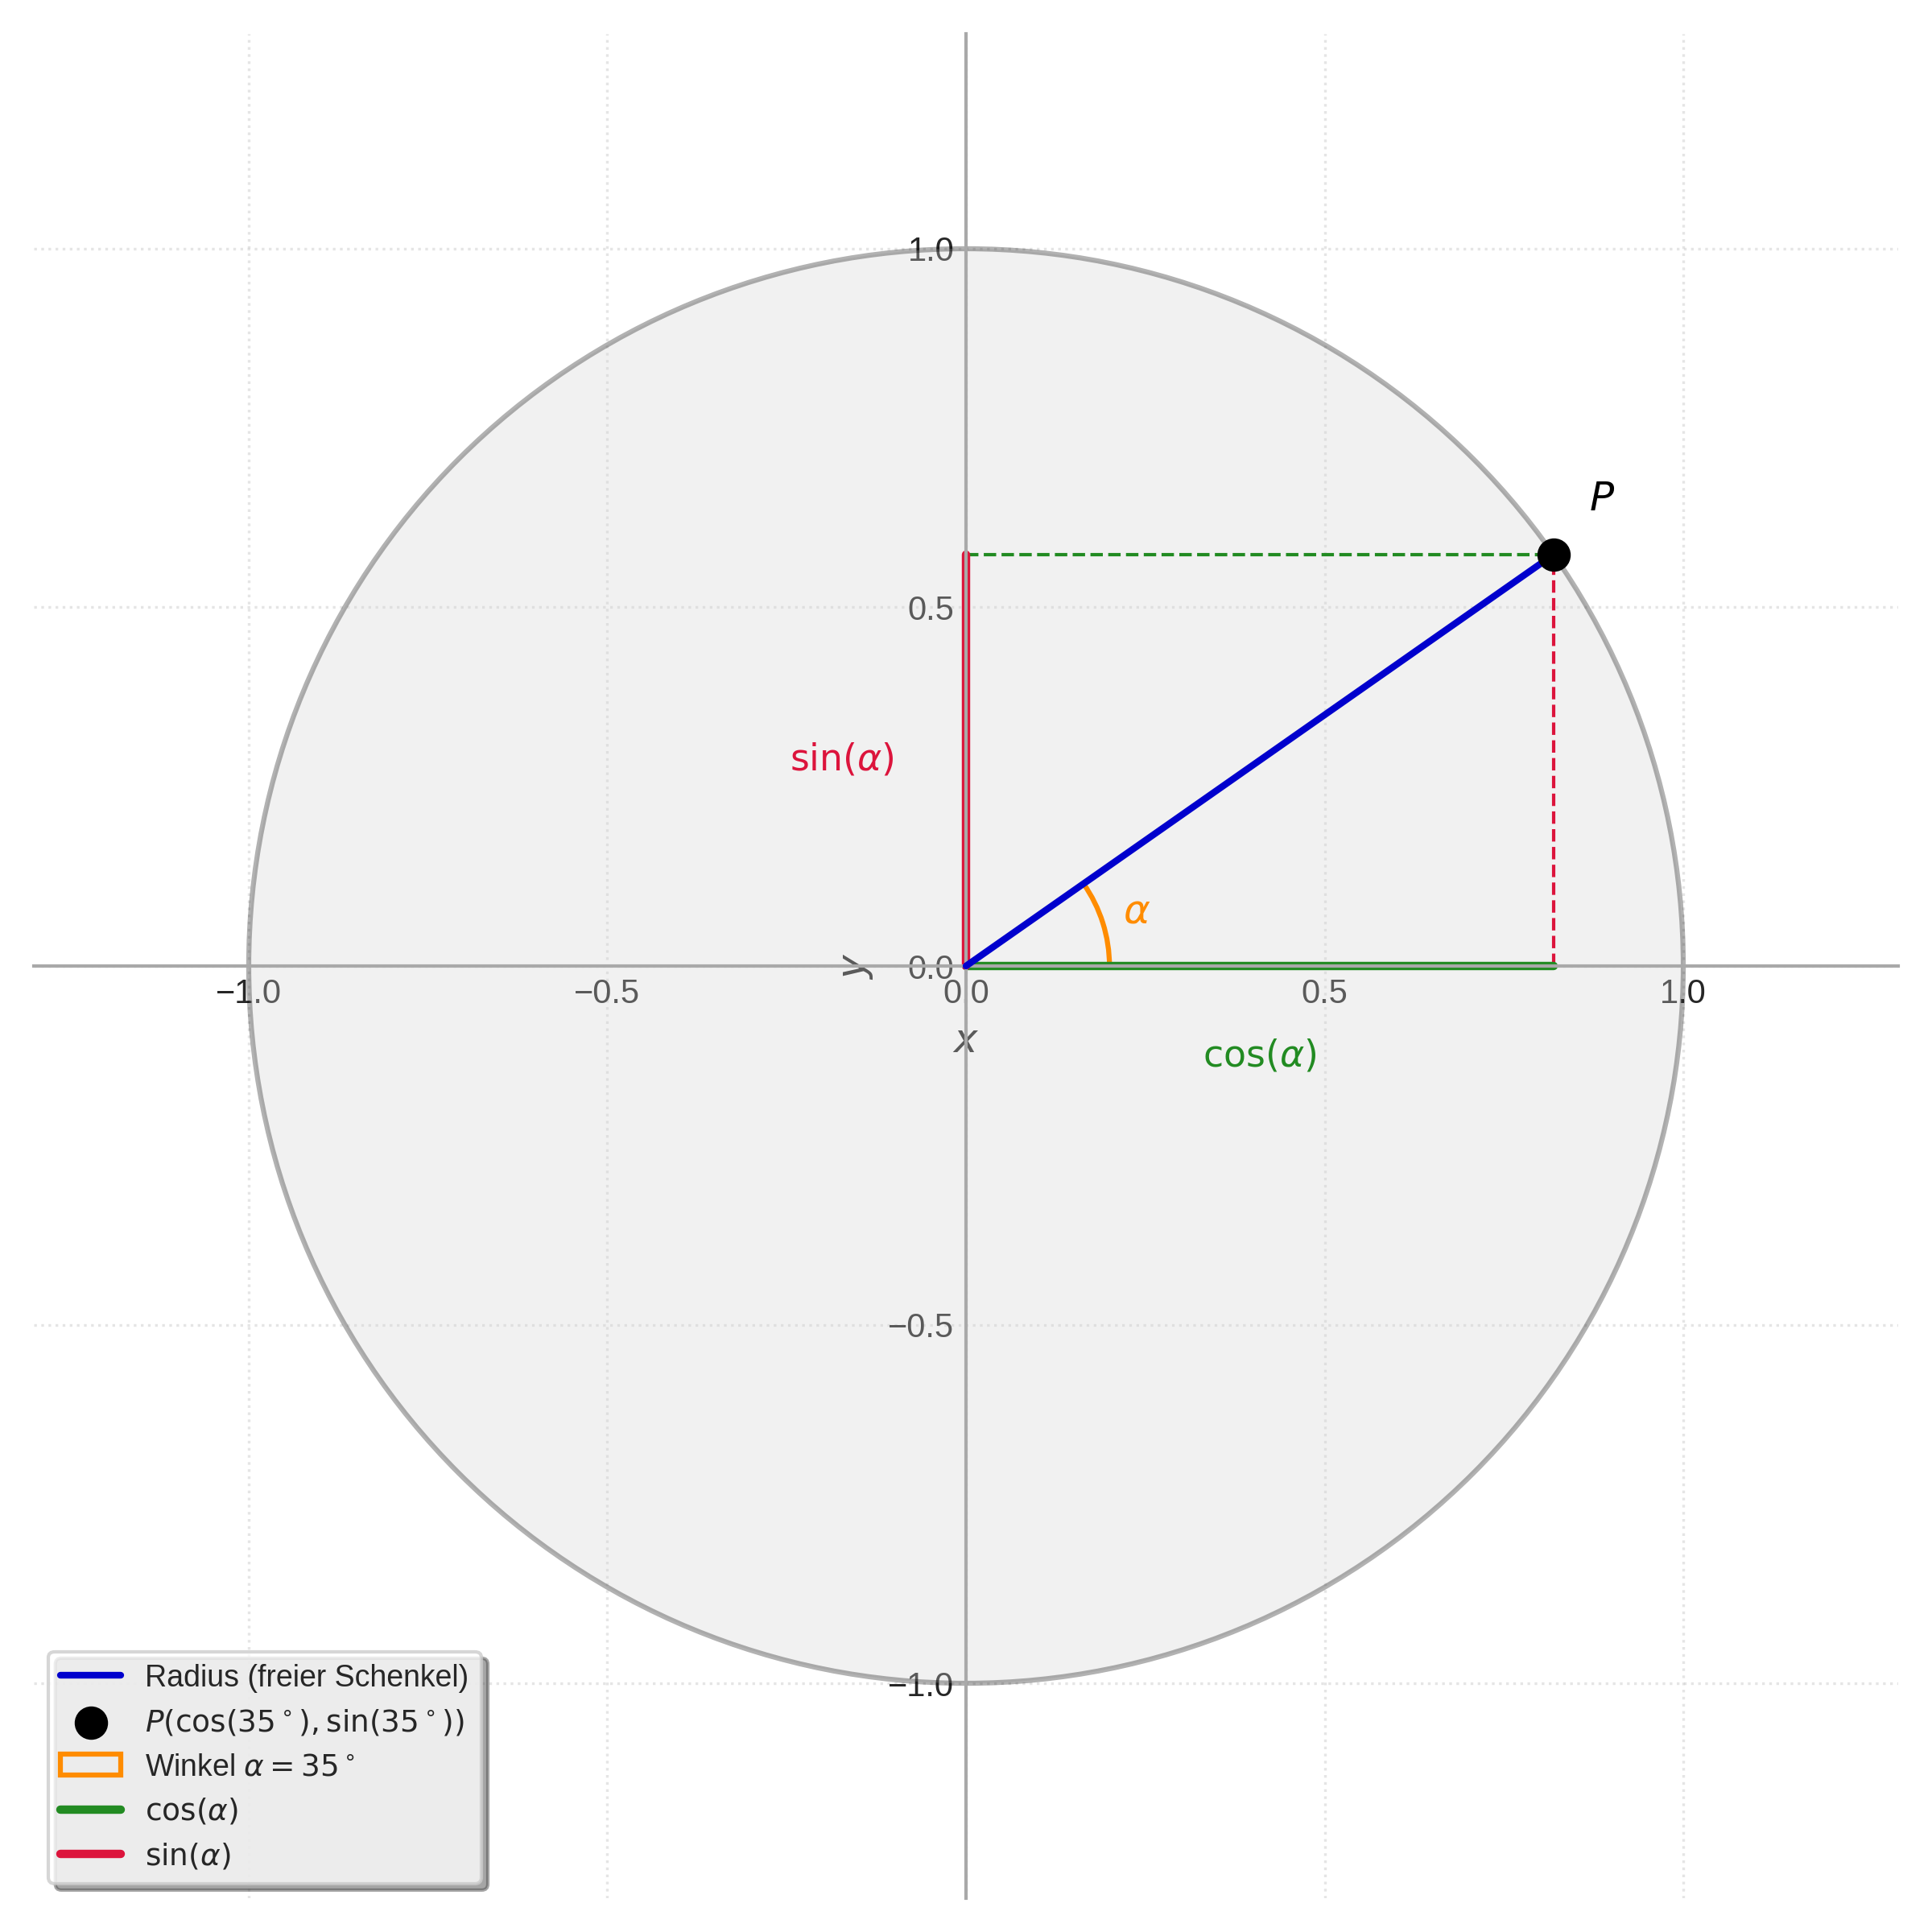
\includegraphics[width=0.7\textwidth]{grafiken/Trig_Einheitskreis.png}
    \captionof{figure}{Definition von Sinus und Kosinus am Einheitskreis}
    \label{fig:einheitskreis}
\end{center}
Aus dieser Definition am Einheitskreis ergeben sich viele wichtige Eigenschaften.

\subsubsection{Graphen und Eigenschaften von $\sin(x)$ und $\cos(x)$}

\begin{merksatzumgebung}{Eigenschaften von $f(x)=\sin(x)$ und $g(x)=\cos(x)$}
\begin{itemize}
    \item \textbf{Definitionsbereich:} $D_f = D_g = \mathbb{R}$ (man kann jeden reellen Winkel einsetzen).
    \item \textbf{Wertebereich:} $W_f = W_g = [-1, 1]$ (die Funktionswerte liegen immer zwischen -1 und 1, inklusive).
    \item \textbf{Periodizität:} Beide Funktionen sind periodisch mit der \textbf{Periode $2\pi$}. Das bedeutet, ihre Werte wiederholen sich alle $2\pi$:
        \[ \sin(x + 2\pi) = \sin(x) \quad \text{und} \quad \cos(x + 2\pi) = \cos(x) \]
    \item \textbf{Nullstellen:}
        \begin{itemize}
            \item $\sin(x) = 0$ für $x = k \cdot \pi$, wobei $k \in \mathbb{Z}$ (alle ganzen Zahlen). Also bei $x=0, \pm\pi, \pm 2\pi, \dots$
            \item $\cos(x) = 0$ für $x = \frac{\pi}{2} + k \cdot \pi$, wobei $k \in \mathbb{Z}$. Also bei $x=\pm\frac{\pi}{2}, \pm\frac{3\pi}{2}, \dots$
        \end{itemize}
    \item \textbf{Extremstellen:}
        \begin{itemize}
            \item $\sin(x)$ hat Maxima ($+1$) bei $x = \frac{\pi}{2} + 2k\pi$ und Minima ($-1$) bei $x = \frac{3\pi}{2} + 2k\pi$.
            \item $\cos(x)$ hat Maxima ($+1$) bei $x = 2k\pi$ und Minima ($-1$) bei $x = \pi + 2k\pi$.
        \end{itemize}
    \item \textbf{Symmetrie:}
        \begin{itemize}
            \item $\sin(x)$ ist \textbf{punktsymmetrisch zum Ursprung}: $\sin(-x) = -\sin(x)$.
            \item $\cos(x)$ ist \textbf{achsensymmetrisch zur y-Achse}: $\cos(-x) = \cos(x)$.
        \end{itemize}
    \item \textbf{Zusammenhang:} Die Graphen von Sinus und Kosinus sind zueinander phasenverschoben:
        $\cos(x) = \sin(x + \frac{\pi}{2})$ (Kosinus ist Sinus um $\pi/2$ nach links verschoben).
        $\sin(x) = \cos(x - \frac{\pi}{2})$ (Sinus ist Kosinus um $\pi/2$ nach rechts verschoben).
    \item \textbf{Wichtiger Grundzusammenhang (Trigonometrischer Pythagoras):} Für jeden Winkel $x$ gilt:
        \[ \sin^2(x) + \cos^2(x) = 1 \]
        (Das folgt direkt aus dem Satz des Pythagoras am Einheitskreis, da $x_P^2+y_P^2=r^2=1^2$).
\end{itemize}
\end{merksatzumgebung}

\begin{center}
    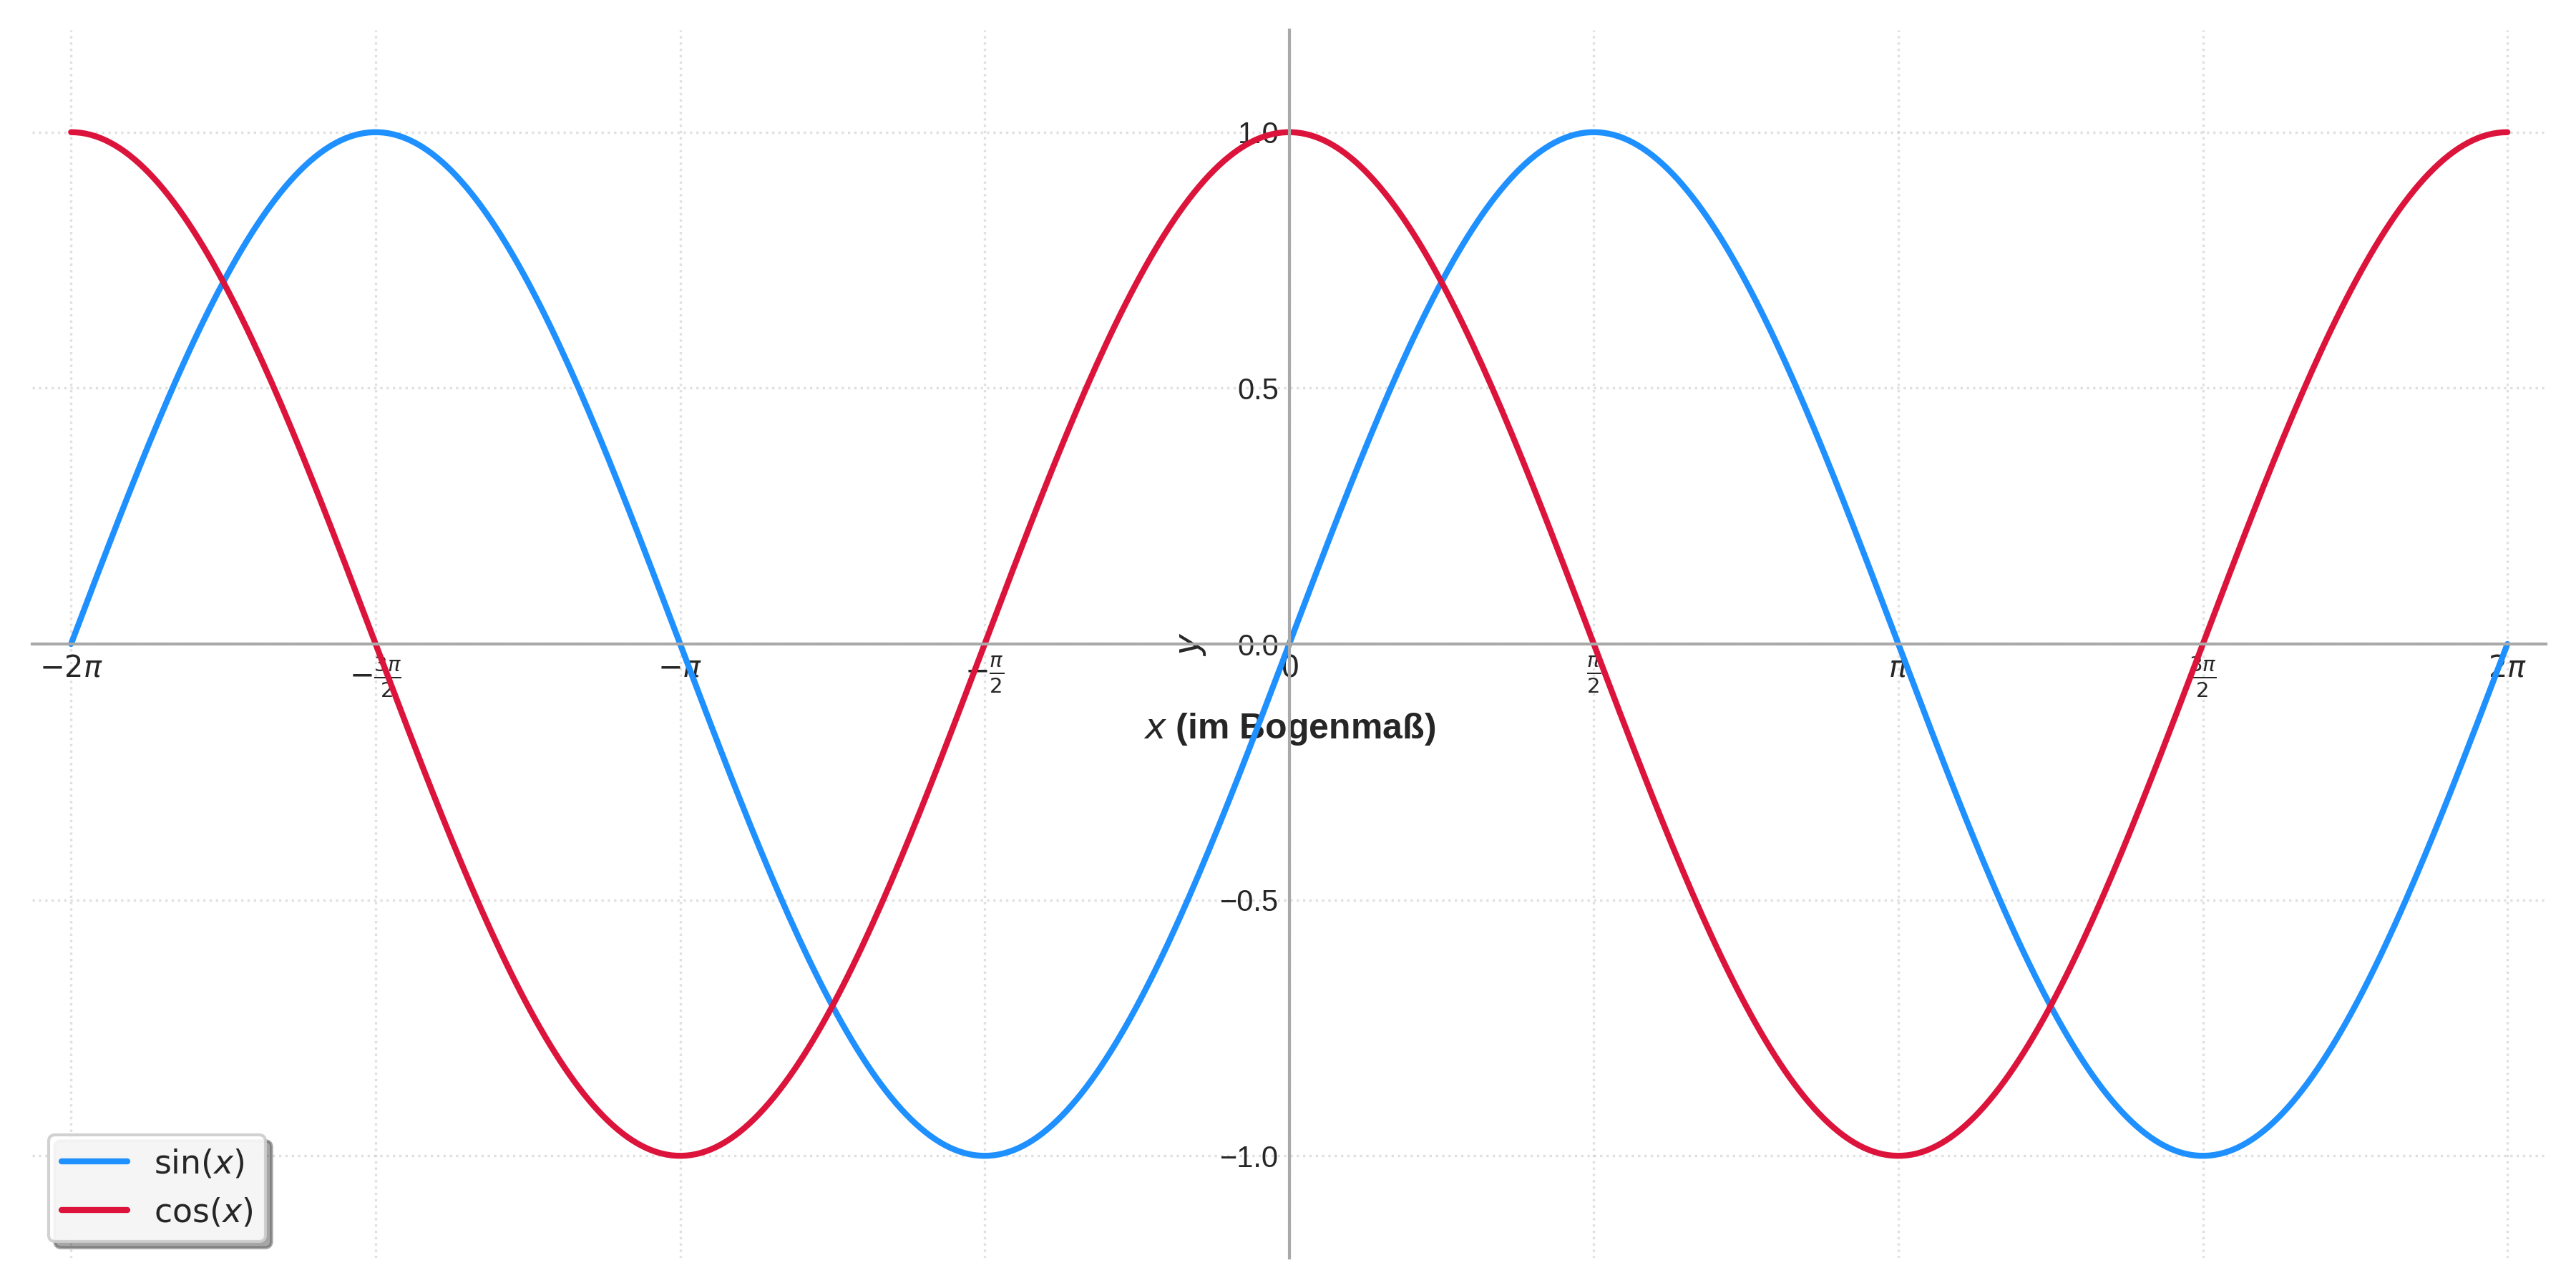
\includegraphics[width=0.9\textwidth]{grafiken/Trig_SinCos_Graphen.png}
    \captionof{figure}{Graphen der Funktionen $f(x)=\sin(x)$ und $g(x)=\cos(x)$}
    \label{fig:sincos_graphen}
\end{center}




\begin{tippumgebung}{Pythagoras im Test – Eine kleine Selbstüberprüfung}
Du hast gerade gelernt, dass für jeden Winkel $x$ gilt: $\sin^2(x) + \cos^2(x) = 1$.
Überlege einmal: Könnte es einen Winkel $x$ geben, für den gleichzeitig $\sin(x) = 0,8$ und $\cos(x) = 0,7$ gilt? Überprüfe dies, indem du die Werte in die Gleichung einsetzt. Was stellst du fest?
(Zur Erinnerung: $\sin^2(x)$ bedeutet $(\sin x)^2$.)
\end{tippumgebung}

% ... (Weiter im Text, z.B. mit der Abbildung der Sinus/Kosinus-Graphen oder dem nächsten Unterabschnitt)
\subsubsection{Ein tieferer Einblick: Sinus und Kosinus als unendliche Reihen (Taylorreihen)}
Eine faszinierende Eigenschaft vieler Funktionen in der Mathematik ist, dass sie als unendliche Summen von Potenzfunktionen dargestellt werden können – sogenannte \textbf{Taylorreihen} (oder Maclaurinreihen, wenn die Entwicklung um den Punkt $x=0$ erfolgt). Für Sinus und Kosinus sehen diese Reihen besonders elegant aus:

\begin{infoboxumgebung}{Taylorreihen für Sinus und Kosinus}
Für alle reellen Zahlen $x$ (im Bogenmaß!) gilt:
\[ \sin(x) = x - \frac{x^3}{3!} + \frac{x^5}{5!} - \frac{x^7}{7!} + \frac{x^9}{9!} - \dots = \sum_{n=0}^{\infty} (-1)^n \frac{x^{2n+1}}{(2n+1)!} \]
\[ \cos(x) = 1 - \frac{x^2}{2!} + \frac{x^4}{4!} - \frac{x^6}{6!} + \frac{x^8}{8!} - \dots = \sum_{n=0}^{\infty} (-1)^n \frac{x^{2n}}{(2n)!} \]
Dabei bedeutet $k!$ (gelesen 'k Fakultät') das Produkt aller ganzen Zahlen von 1 bis $k$: $k! = 1 \cdot 2 \cdot 3 \cdot \dots \cdot k$. (Und $0!=1$).
Zum Beispiel: $3! = 1 \cdot 2 \cdot 3 = 6$, $5! = 1 \cdot 2 \cdot 3 \cdot 4 \cdot 5 = 120$.

\textbf{Was bedeuten diese Reihen?}
\begin{itemize}
    \item Sie zeigen, dass Sinus und Kosinus im Grunde 'unendlich lange Polynome' sind.
    \item Man kann mit diesen Reihen die Werte von $\sin(x)$ und $\cos(x)$ für jedes $x$ beliebig genau annähern, indem man genügend Glieder der Summe berücksichtigt. So berechnen auch Taschenrechner diese Werte!
    \item Aus diesen Reihen lassen sich viele Eigenschaften der Funktionen ableiten, z.B. ihre Ableitungen.
\end{itemize}
Die Herleitung dieser Reihen ist fortgeschrittene Mathematik, aber ihre Existenz zu kennen, öffnet ein Fenster zu tieferen Zusammenhängen.
\end{infoboxumgebung}

\textit{Selbst-Check:} Setze $x=0$ in die Reihen für $\sin(x)$ und $\cos(x)$ ein. Was erhältst du? Vergleiche mit $\sin(0)$ und $\cos(0)$ vom Einheitskreis. (Antwort: $\sin(0)=0$, $\cos(0)=1$. Das passt!)
\begin{funfactbox}{$\pi$ aus dem Nichts? Eine unendliche Summe enthüllt die Kreiszahl!}
Die Kreiszahl $\pi \approx 3,14159\dots$ ist dir sicher bekannt. Sie beschreibt das Verhältnis des Umfangs eines Kreises zu seinem Durchmesser. Aber wie kommt man eigentlich auf diese unendlich vielen Nachkommastellen? Es gibt viele faszinierende Wege, $\pi$ zu berechnen, und einige davon haben Verbindungen zur Differential- und Integralrechnung!

Eine berühmte Methode verwendet eine unendliche Summe, die mit dem Mathematiker Gottfried Wilhelm Leibniz (einem der 'Erfinder' der Differentialrechnung) in Verbindung gebracht wird, aber auch schon früher in Indien bekannt war:
\[ \frac{\pi}{4} = 1 - \frac{1}{3} + \frac{1}{5} - \frac{1}{7} + \frac{1}{9} - \frac{1}{11} + \dots \]
Das ist die sogenannte \textbf{Leibniz-Reihe}. Sie besagt, dass man sich dem Wert von $\pi/4$ immer genauer annähert, je mehr Terme dieser abwechselnden (alternierenden) Reihe man addiert und subtrahiert. Multipliziert man das Ergebnis mit 4, erhält man eine Annäherung für $\pi$.

\textbf{Wo steckt da die Verbindung zur Analysis?}
Diese Reihe ist eigentlich ein Spezialfall der Taylorreihe für die Funktion $f(x) = \arctan(x)$ (Arkustangens, die Umkehrfunktion des Tangens), ausgewertet an der Stelle $x=1$, denn $\arctan(1) = \frac{\pi}{4}$.
Die Taylorreihe einer Funktion ist eine Darstellung dieser Funktion als unendliche Summe von Potenztermen, wobei die Koeffizienten dieser Terme durch die \textbf{Ableitungen} der Funktion an einem bestimmten Punkt bestimmt werden.

Man kann zeigen:
\[ \arctan(x) = x - \frac{x^3}{3} + \frac{x^5}{5} - \frac{x^7}{7} + \dots \]
Setzt man hier $x=1$ ein, erhält man genau die Leibniz-Reihe für $\frac{\pi}{4}$.

Die Herleitung solcher unendlicher Reihen für Funktionen ist ein wichtiges Anwendungsfeld der Differential- (und auch der Integral-) rechnung. Sie zeigt, wie man komplexe Zahlen wie $\pi$ oder Funktionswerte durch einfachere Bausteine (Potenzen) annähern und berechnen kann. Auch wenn diese spezielle Reihe für die praktische Berechnung von $\pi$ nicht sehr schnell konvergiert (man braucht viele Terme für eine gute Genauigkeit), ist sie ein wunderschönes Beispiel für die tiefen Verbindungen in der Mathematik!

\begin{center}
    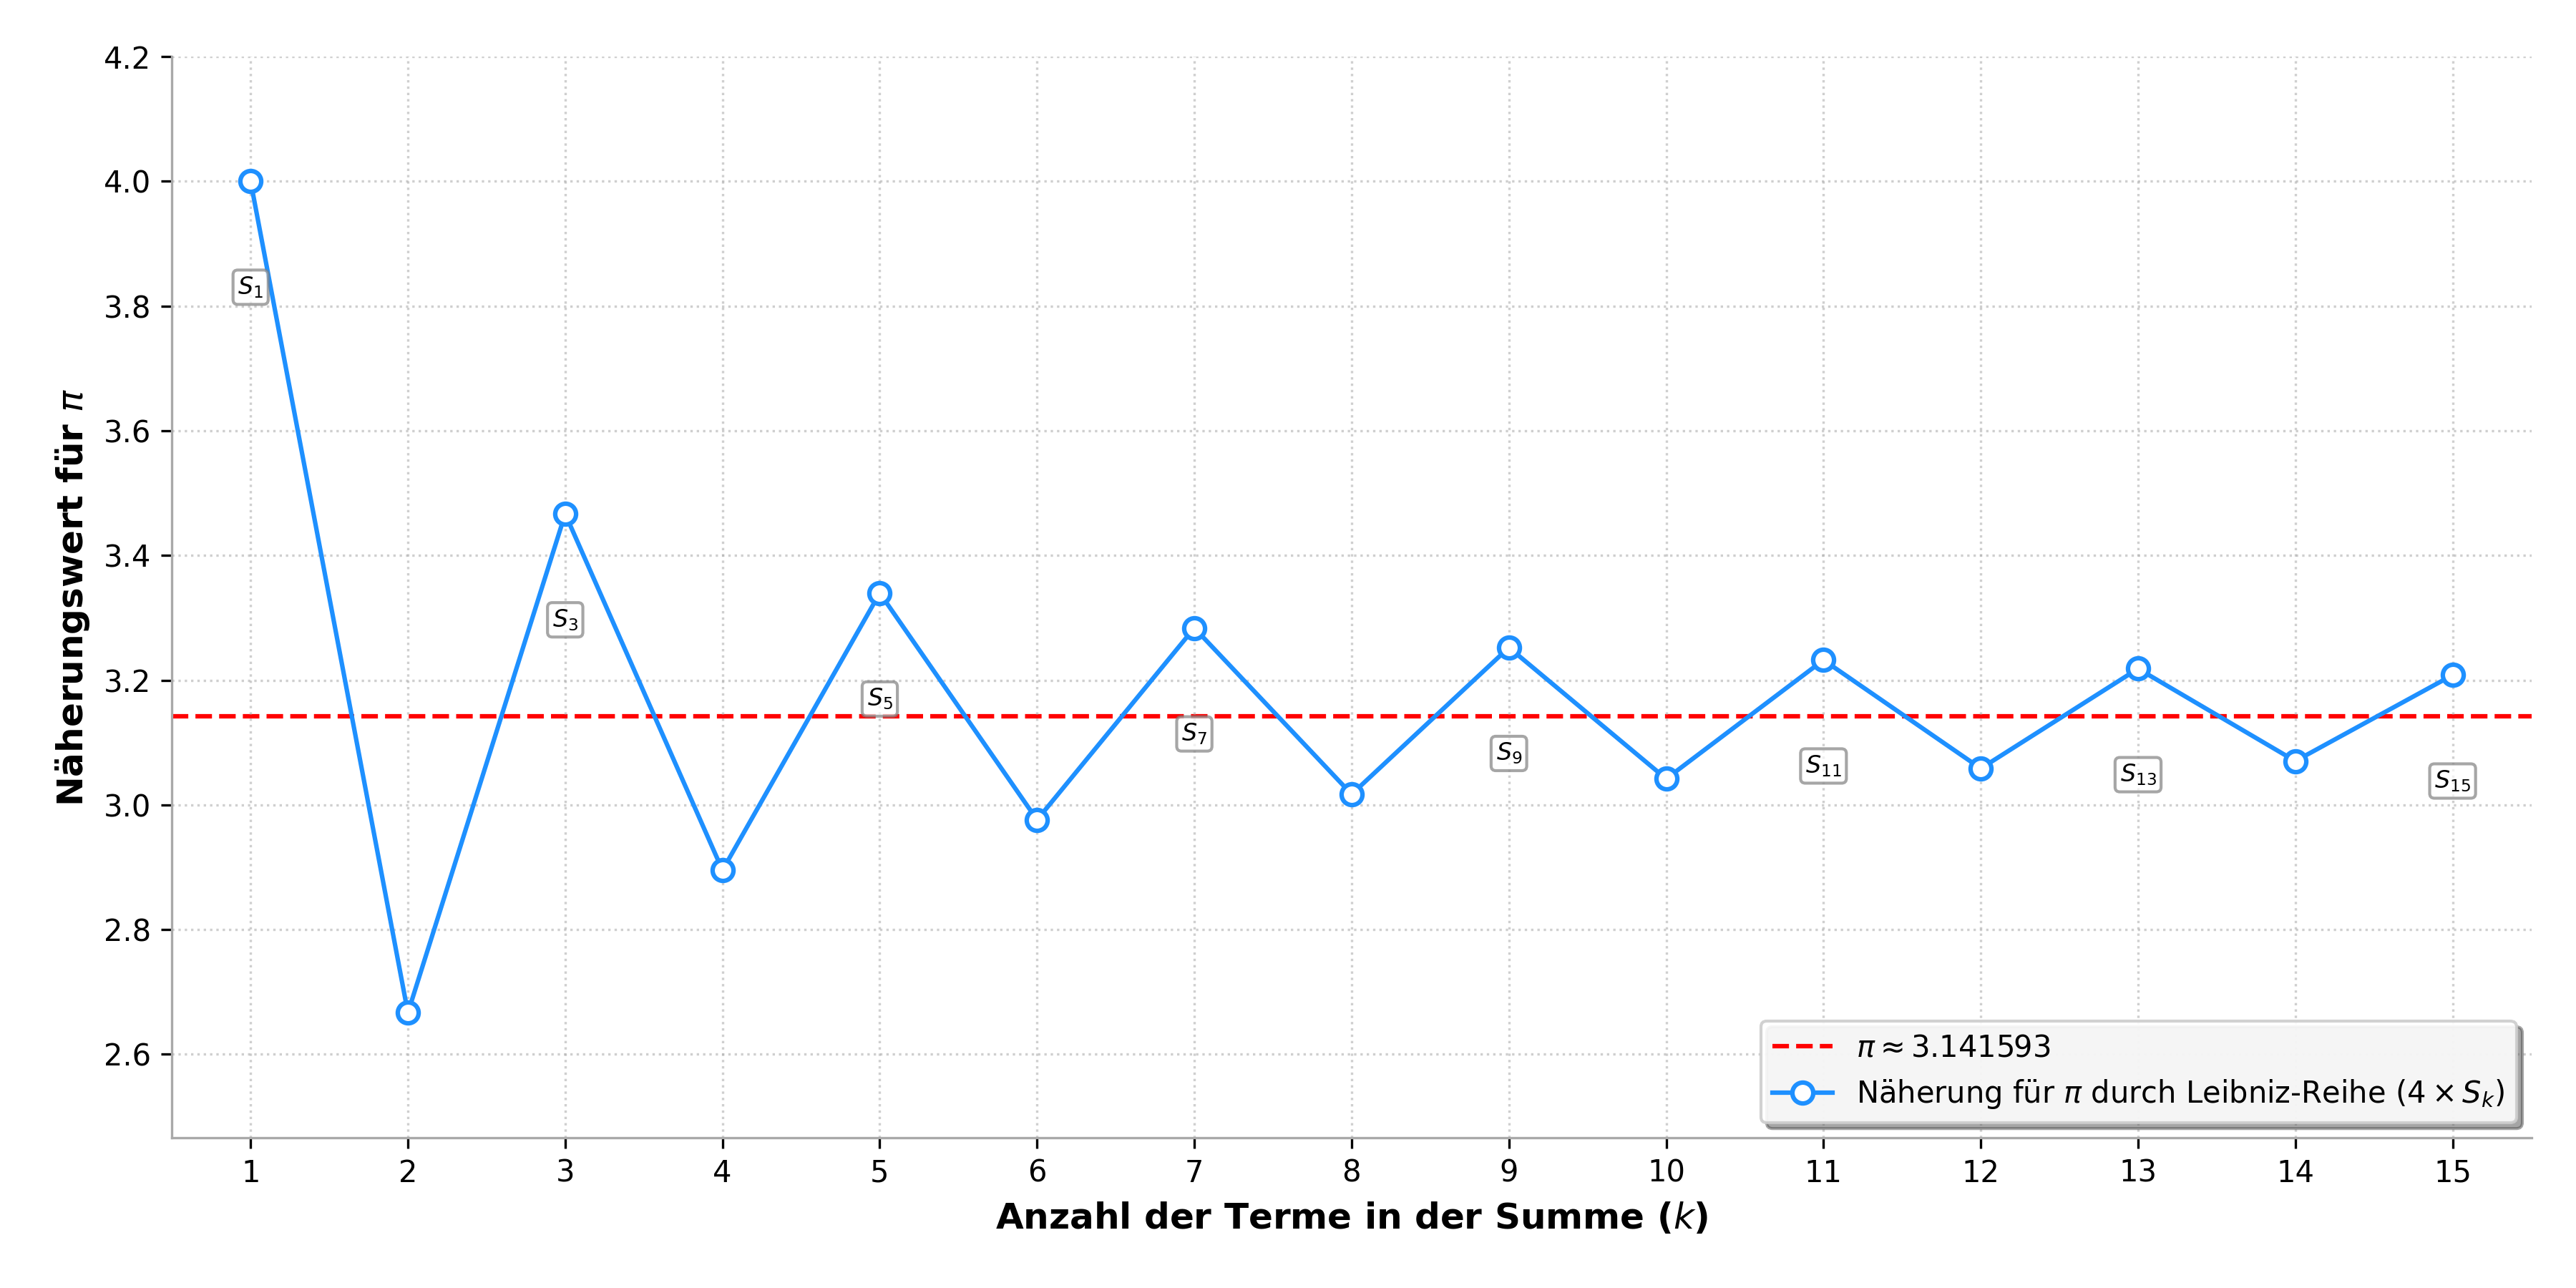
\includegraphics[width=0.8\textwidth]{grafiken/Pi_Leibniz_Reihe.png}
    % Beschreibung für die Grafik 'Pi_Leibniz_Reihe.png':
    % Die Grafik könnte visualisieren, wie sich die Summe der ersten Terme 
    % der Leibniz-Reihe (multipliziert mit 4) langsam dem Wert von Pi annähert.
    % Z.B. ein Zahlenstrahl, auf dem die Näherungswerte für S_1, S_2, S_3 etc. 
    % aufgetragen sind und wie sie um Pi 'oszillieren' und sich annähern.
    % Alternativ: Eine stilisierte Darstellung der Zahl Pi mit der Leibniz-Reihe daneben.
    \captionof{figure}{Annäherung an $\pi$ durch die Leibniz-Reihe (konzeptionelle Darstellung)}
    \label{fig:pi_leibniz_funfact}
\end{center}
\end{funfactbox}

\subsubsection{Ableitungen von Sinus und Kosinus}
Eine der schönsten Symmetrien in der Differentialrechnung findet sich bei den Ableitungen von Sinus und Kosinus.

\begin{infoboxumgebung}{Beobachtung: Steigung von $\sin x$ und Werte von $\cos x$}
Bevor wir die Ableitungsregeln für Sinus und Kosinus formal kennenlernen, lass uns eine kleine Beobachtung am Graphen von $f(x)=\sin(x)$ und $g(x)=\cos(x)$ machen (siehe Abbildung \ref{fig:sincos_graphen}):
\begin{itemize}
    \item Wo hat der Graph von $\sin(x)$ seine Hoch- und Tiefpunkte? Welche Steigung hat der Graph an diesen Stellen offensichtlich? Welchen Wert hat $\cos(x)$ an genau diesen x-Stellen?
    \item Wo schneidet der Graph von $\sin(x)$ die x-Achse mit positiver Steigung (z.B. bei $x=0, 2\pi, \dots$)? Welchen Wert hat $\cos(x)$ dort? Wo ist die Steigung von $\sin(x)$ am größten?
    \item Wo schneidet der Graph von $\sin(x)$ die x-Achse mit negativer Steigung (z.B. bei $x=\pi, 3\pi, \dots$)? Welchen Wert hat $\cos(x)$ dort? Wo ist die Steigung von $\sin(x)$ am stärksten negativ (also betragsmäßig am größten, aber negativ)?
\end{itemize}
Vielleicht erkennst du schon ein Muster im Zusammenhang zwischen der Steigung von $\sin(x)$ und den Funktionswerten von $\cos(x)$. Genau diesen Zusammenhang werden wir mit der Ableitung präzisieren!
\end{infoboxumgebung}

\begin{merksatzumgebung}{Ableitungen von $\sin(x)$ und $\cos(x)$}
Für Winkel $x$ im Bogenmaß gilt:
\begin{itemize}
    \item Die Ableitung von $f(x) = \sin(x)$ ist $f'(x) = \cos(x)$.
    \[ (\sin x)' = \cos x \]
    \item Die Ableitung von $g(x) = \cos(x)$ ist $g'(x) = -\sin(x)$.
    \[ (\cos x)' = -\sin x \]
\end{itemize}
\end{merksatzumgebung}

\begin{tippumgebung}{Ableitungen aus den Taylorreihen (für Interessierte)}
Wenn man die Taylorreihen von $\sin(x)$ und $\cos(x)$ Glied für Glied mit der Potenzregel ableitet (was bei Potenzreihen unter bestimmten Bedingungen erlaubt ist), erhält man genau diese Ableitungsregeln!
Beispiel für Sinus:
$\sin(x) = x - \frac{x^3}{3!} + \frac{x^5}{5!} - \frac{x^7}{7!} + \dots$
$(\sin(x))' = (x)' - (\frac{x^3}{6})' + (\frac{x^5}{120})' - \dots$
$= 1 - \frac{3x^2}{6} + \frac{5x^4}{120} - \dots$
$= 1 - \frac{x^2}{2} + \frac{x^4}{24} - \dots$
$= 1 - \frac{x^2}{2!} + \frac{x^4}{4!} - \dots = \cos(x)$!
\end{tippumgebung}

Mit diesen Ableitungen können wir nun auch die höheren Ableitungen bestimmen:
\begin{itemize}
    \item $f(x) = \sin(x)$
    \item $f'(x) = \cos(x)$
    \item $f''(x) = (\cos x)' = -\sin(x)$
    \item $f'''(x) = (-\sin x)' = -(\cos x) = -\cos(x)$
    \item $f^{(4)}(x) = (-\cos x)' = -(-\sin x) = \sin(x)$
\end{itemize}
Nach der vierten Ableitung wiederholt sich der Zyklus! Das Gleiche gilt für $\cos(x)$.

\subsubsection{Stammfunktionen von Sinus und Kosinus}
Aus den Ableitungsregeln ergeben sich direkt die Stammfunktionen:

\begin{merksatzumgebung}{Stammfunktionen von $\sin(x)$ und $\cos(x)$}
\begin{itemize}
    \item Eine Stammfunktion von $f(x) = \cos(x)$ ist $F(x) = \sin(x)$, denn $(\sin x)' = \cos x$.
    Also: \[\int \cos(x) \,dx = \sin(x) + C \]
    \item Eine Stammfunktion von $g(x) = \sin(x)$ ist $G(x) = -\cos(x)$, denn $(-\cos x)' = -(-\sin x) = \sin x$.
    Also: \[\int \sin(x) \,dx = -\cos(x) + C \]
\end{itemize}
Achte auf das Minuszeichen bei der Stammfunktion von $\sin(x)$!
\end{merksatzumgebung}

\begin{beispielumgebung}{Ableiten und Integrieren mit $\sin x$ und $\cos x$}
\begin{enumerate}
    \item Leite $f(x) = 3\sin(x) - 2\cos(x) + x^2$ ab.
        $f'(x) = (3\sin x)' - (2\cos x)' + (x^2)'$
        $f'(x) = 3\cos(x) - 2(-\sin x) + 2x = 3\cos(x) + 2\sin(x) + 2x$.
    \item Bestimme $\int (4\cos(x) + \sin(x) - 2) \,dx$.
        $\int (4\cos(x) + \sin(x) - 2) \,dx = 4\int\cos(x)dx + \int\sin(x)dx - \int 2dx$
        $= 4\sin(x) + (-\cos x) - 2x + C = 4\sin(x) - \cos(x) - 2x + C$.
\end{enumerate}
\end{beispielumgebung}

\begin{aufgabenumgebung}{Erste Übungen mit $\sin x$ und $\cos x$}
\begin{enumerate}
    \item Bilde die erste und zweite Ableitung der folgenden Funktionen:
        \begin{itemize}
            \item $f_1(x) = -5\cos(x) + 2\sin(x) - e^x$
            \item $f_2(x) = \sin(x) + \ln(x)$ (Beachte den Definitionsbereich!)
        \end{itemize}
    \item Bestimme die Menge aller Stammfunktionen:
        \begin{itemize}
            \item $g_1(x) = \frac{1}{2}\sin(x) - 3\cos(x) + x^3$
            \item $g_2(x) = \cos(x) - \frac{1}{x}$
        \end{itemize}
    \item Berechne das bestimmte Integral $\int_0^{\pi} \sin(x) \,dx$. Was stellt dieser Wert geometrisch dar? Skizziere den Graphen von $\sin(x)$ im Intervall $[0, 2\pi]$ und markiere die berechnete Fläche.
    \item Was ist $\int_0^{2\pi} \sin(x) \,dx$? Erkläre das Ergebnis anhand der Symmetrie und der orientierten Fläche.
\end{enumerate}
\end{aufgabenumgebung}

% Vorheriger Inhalt des Kapitels bis zur aufgabenumgebung 'Erste Übungen mit sin x und cos x'
% ... (siehe vorherige Canvas-Version) ...

% Hier geht es dann weiter mit Transformationen von sin/cos, Tangens, 
% Anwendung der Produkt-/Quotienten-/Kettenregel und Kurvendiskussionen.
% Dieser Kommentar wird durch den folgenden Inhalt ersetzt:

\subsection{Transformationen von Sinus- und Kosinusfunktionen}
\label{subsec:trafo_sincos}

Die Grundfunktionen $f(x)=\sin(x)$ und $g(x)=\cos(x)$ können durch verschiedene Parameter verändert (transformiert) werden, um eine größere Vielfalt an periodischen Vorgängen zu modellieren. Die allgemeine Form einer transformierten Sinusfunktion (analog für Kosinus) ist:
\[ f(x) = A \cdot \sin(B(x-C)) + D \]
oder auch oft geschrieben als:
\[ f(x) = A \cdot \sin(Bx - \varphi) + D \quad \text{mit } \varphi = B \cdot C \]

\begin{merksatzumgebung}{Parameter der allgemeinen Sinusfunktion $f(x) = A \sin(B(x-C)) + D$}
\begin{itemize}
    \item \textbf{Amplitude $|A|$:}
        \begin{itemize}
            \item Der Faktor $A$ streckt oder staucht den Graphen in y-Richtung.
            \item $|A|$ ist die \textbf{Amplitude}, d.h. die maximale Auslenkung von der Mittellage. Der Wertebereich ist $[D-|A|, D+|A|]$.
            \item Wenn $A < 0$, wird der Graph zusätzlich an der Mittellage (Gerade $y=D$) gespiegelt.
        \end{itemize}
    \item \textbf{Periode $P$ (beeinflusst durch $B$):}
        \begin{itemize}
            \item Der Faktor $B$ beeinflusst die Periode der Schwingung. $B$ wird auch Kreisfrequenz genannt (oft als $\omega$ bezeichnet).
            \item Die \textbf{Periode} $P$ (die Länge einer vollständigen Schwingung) berechnet sich als:
            \[ P = \frac{2\pi}{|B|} \]
            \item Wenn $|B|>1$, wird die Periode kürzer (die Schwingung ist 'schneller', gestaucht in x-Richtung).
            \item Wenn $0<|B|<1$, wird die Periode länger (die Schwingung ist 'langsamer', gestreckt in x-Richtung).
            \item \textit{Zum Weiterdenken:} Was passiert anschaulich mit der Periode $P$, wenn der Betrag von $B$ sehr groß wird (z.B. $|B|=100$)? Die Schwingung wird dann sehr \dots (schnell/kurz oder langsam/lang)? Und was passiert, wenn $|B|$ sehr klein (aber positiv) wird (z.B. $|B|=0.1$)? Die Schwingung wird dann sehr \dots? Passt das zu deiner Vorstellung von 'gestaucht' bzw. 'gestreckt' in x-Richtung?
        \end{itemize}
    \item \textbf{Verschiebung in x-Richtung (Phasenverschiebung $C$):}
        \begin{itemize}
            \item Der Parameter $C$ bewirkt eine Verschiebung des Graphen entlang der x-Achse.
            \item Wenn $C>0$ (also im Term $(x-C)$), wird der Graph um $C$ Einheiten nach \textbf{rechts} verschoben.
            \item Wenn $C<0$ (also im Term $(x+ |C|)$), wird der Graph um $|C|$ Einheiten nach \textbf{links} verschoben.
            \item Diese Verschiebung wird auch \textbf{Phasenverschiebung} genannt.
        \end{itemize}
    \item \textbf{Verschiebung in y-Richtung (Mittellage $D$):}
        \begin{itemize}
            \item Der Parameter $D$ verschiebt den gesamten Graphen um $D$ Einheiten in y-Richtung.
            \item Die Gerade $y=D$ ist die neue \textbf{Mittellage} oder Ruhelage der Schwingung.
        \end{itemize}
\end{itemize}
Die gleichen Interpretationen gelten für die Kosinusfunktion $f(x) = A \cos(B(x-C)) + D$.
\end{merksatzumgebung}

\begin{beispielumgebung}{Analyse einer transformierten Sinusfunktion}
Betrachte die Funktion $f(x) = 2 \sin\left(0.5(x - \frac{\pi}{2})\right) + 1$.
\begin{itemize}
    \item \textbf{Amplitude $A$:} $A=2$. Die maximale Auslenkung von der Mittellage ist 2.
    \item \textbf{Parameter $B$ und Periode $P$:} $B=0.5$. Die Periode ist $P = \frac{2\pi}{|0.5|} = \frac{2\pi}{1/2} = 4\pi$. Die Schwingung ist also langsamer als die Grundschwingung.
    \item \textbf{Verschiebung in x-Richtung $C$:} $C=\frac{\pi}{2}$. Der Graph der Sinusfunktion $2\sin(0.5x)$ wird um $\frac{\pi}{2}$ nach rechts verschoben.
    \item \textbf{Verschiebung in y-Richtung $D$:} $D=1$. Die Mittellage ist die Gerade $y=1$.
    \item \textbf{Wertebereich:} Die Mittellage ist $y=1$, die Amplitude ist $2$. Also schwingt die Funktion zwischen $1-2=-1$ und $1+2=3$. Der Wertebereich ist $[-1, 3]$.
\end{itemize}
\begin{center}
    % Platzhalter für die Grafik 'Transformierte Sinusfunktion'
    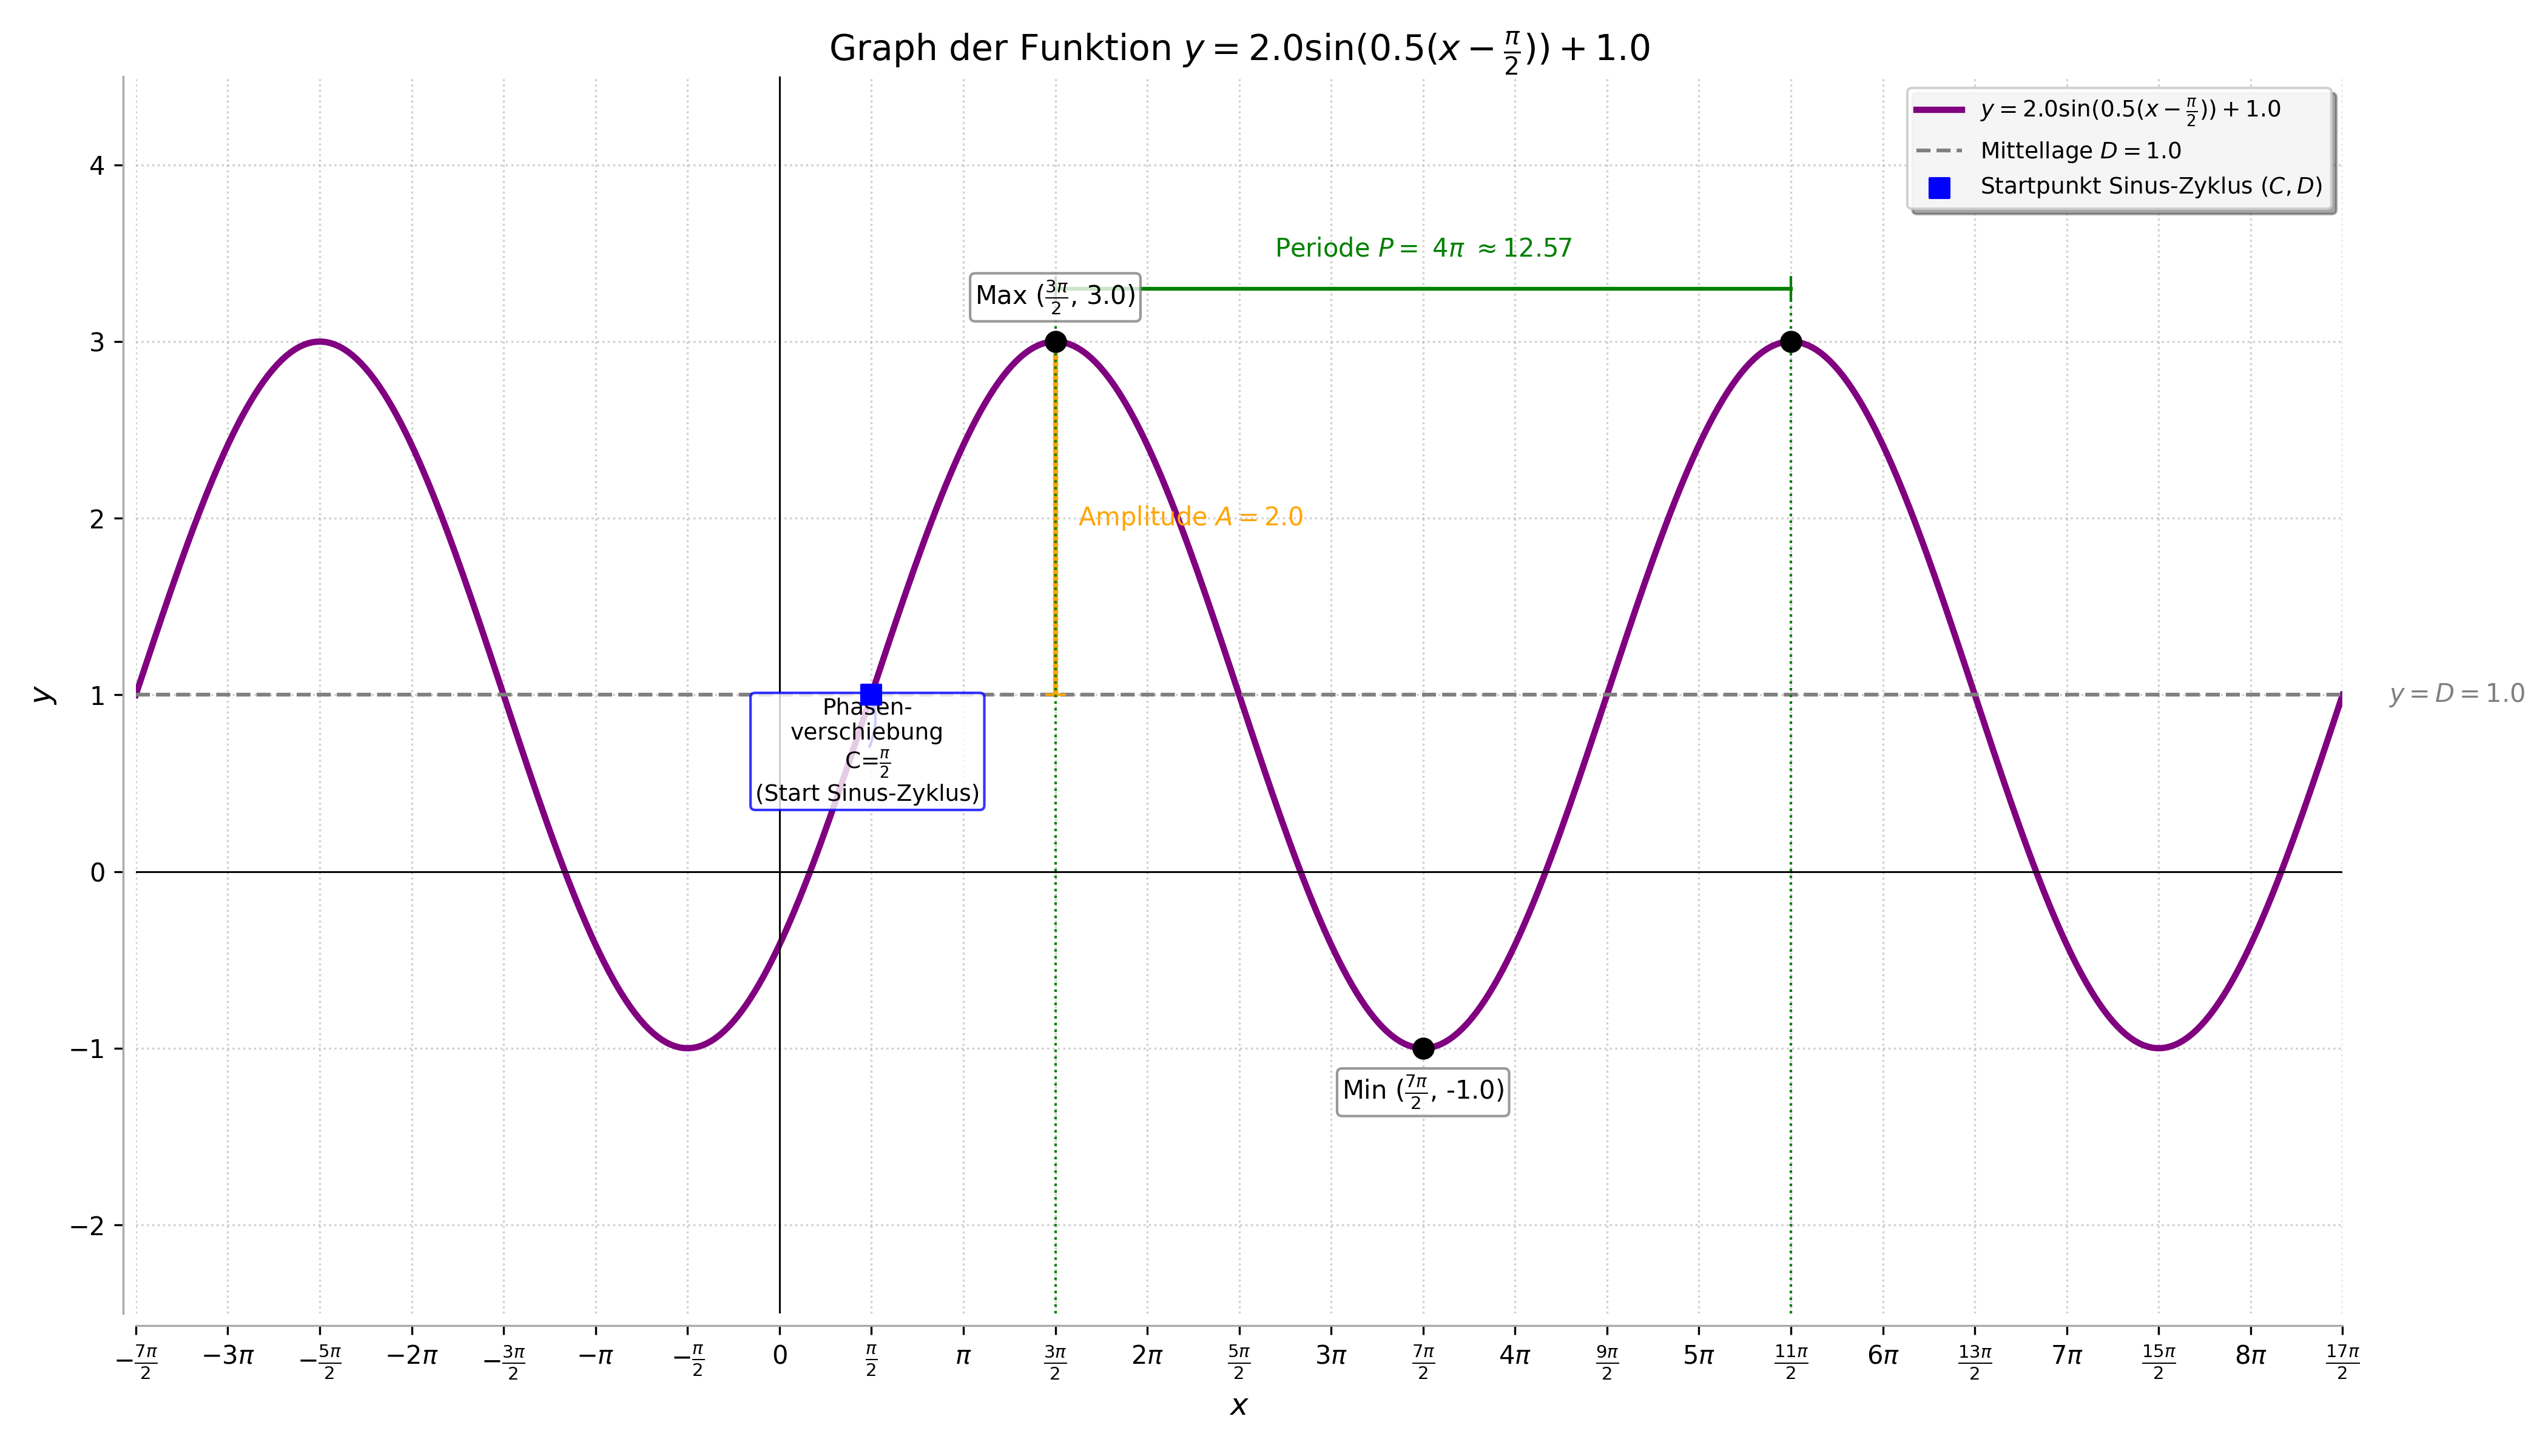
\includegraphics[width=0.9\textwidth]{grafiken/Trig_Trafo_Sinus.png}
    \captionof{figure}{Graph der transformierten Sinusfunktion.}
    \label{fig:trafo_sin}
\end{center}
\end{beispielumgebung}

\begin{fehlerboxumgebung}{Trigonometrische Funktionen – Typische Fallstricke}
Beim Rechnen mit Sinus, Kosinus und Co. gibt es einige typische Fehlerquellen:
\begin{itemize}
    \item \textbf{Gradmaß vs. Bogenmaß:} Die Ableitungs- und Integrationsregeln $(\sin x)'=\cos x$ etc. gelten \textbf{nur}, wenn $x$ im Bogenmaß angegeben ist! Viele Taschenrechner sind standardmäßig auf Gradmaß (DEG) eingestellt. Für die Analysis muss er auf Radiant (RAD) umgestellt sein, sonst sind numerische Ergebnisse falsch.
    \item \textbf{Vorzeichen bei Ableitungen/Stammfunktionen:} Merke dir gut: $(\cos x)' = \mathbf{-}\sin x$ und $\int \sin x \,dx = \mathbf{-}\cos x + C$. Diese Minuszeichen werden oft vergessen!
    \item \textbf{Parameter bei Transformationen falsch interpretiert:}
        \begin{itemize}
            \item Bei $A \sin(B(x-C))+D$: Die Periode ist $P=\frac{2\pi}{|B|}$, nicht $2\pi \cdot B$ oder Ähnliches.
            \item Die Phasenverschiebung bei $B(x-C)$ ist $C$ nach rechts. Steht z.B. $\sin(2x-\pi)$, musst du erst $2$ ausklammern zu $\sin(2(x-\frac{\pi}{2}))$, um die korrekte Phasenverschiebung $C=\frac{\pi}{2}$ nach rechts zu erkennen.
        \end{itemize}
    \item \textbf{Definitionsbereich von $\tan x$ ignoriert:} $\tan x$ ist nicht für $x = \frac{\pi}{2} + k\pi$ definiert. An diesen Stellen sind Polstellen (senkrechte Asymptoten).
    \item \textbf{Verwechslung von $\sin^2 x$ mit $\sin(x^2)$:} $\sin^2 x = (\sin x)^2$, während $\sin(x^2)$ bedeutet, dass zuerst $x$ quadriert und dann der Sinus davon genommen wird. Beim Ableiten erfordern sie unterschiedliche Anwendungen der Kettenregel.
\end{itemize}
Achte auf diese Punkte, um typische Fehler zu vermeiden!
\end{fehlerboxumgebung}

\begin{aufgabenumgebung}{Transformierte Sinus- und Kosinusfunktionen}
\begin{enumerate}
    \item Bestimme für die folgenden Funktionen Amplitude, Periode, Phasenverschiebung (Richtung und Betrag) und Verschiebung in y-Richtung. Gib den Wertebereich an.
        \begin{itemize}
            \item $f_1(x) = 3 \cos(2x - \pi) - 1$ (Tipp: Klammere zuerst den Faktor vor dem $x$ in der Klammer aus, um die Form $B(x-C)$ zu erhalten: $2x-\pi = 2(x-\frac{\pi}{2})$)
            \item $f_2(x) = -0.5 \sin(\pi x + \frac{\pi}{4}) + 2$
            \item $f_3(t) = 100 \cos(2\pi \cdot 50 t)$ (Modell für Wechselspannung)
        \end{itemize}
    \item Skizziere den Graphen von $g(x) = \sin(2(x+\frac{\pi}{4}))$ für eine Periode. Beginne mit dem Graphen von $\sin(x)$ und führe die Transformationen schrittweise durch.
    \item Gegeben ist ein Graph einer Sinusfunktion. Bestimme aus dem Graphen die Parameter $A, B, C, D$ und stelle eine mögliche Funktionsgleichung auf.
        \begin{center}
            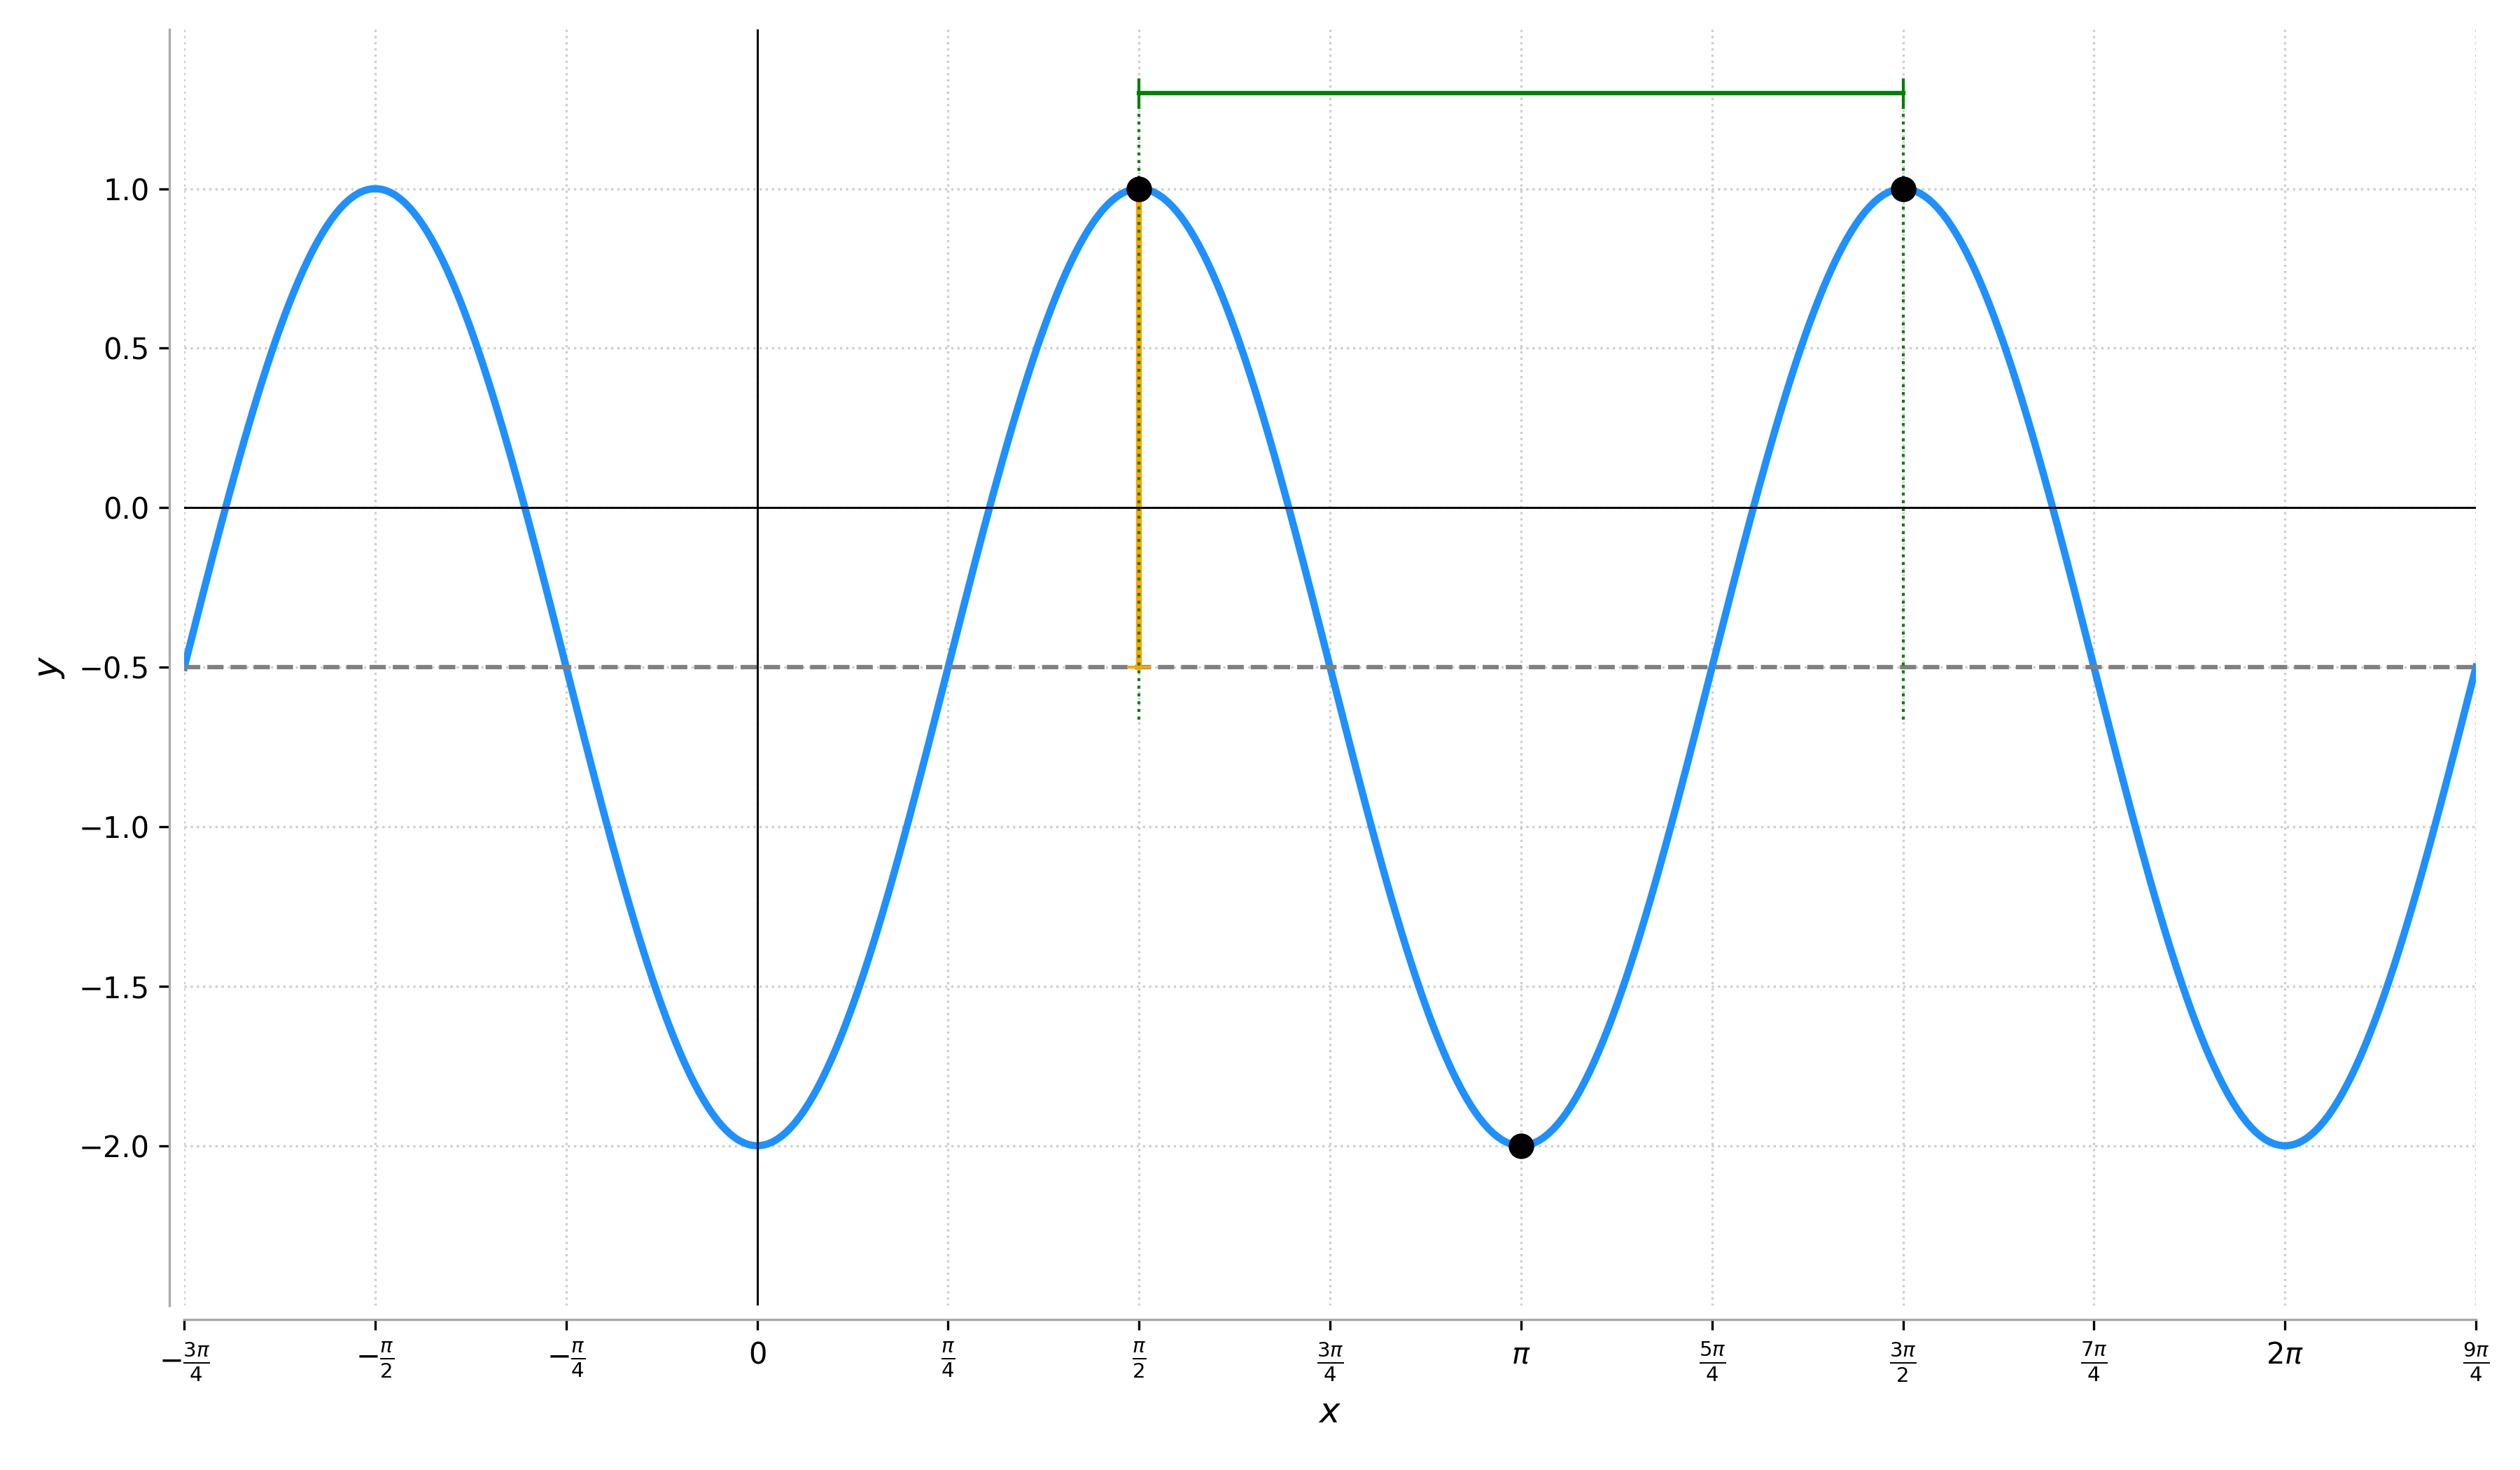
\includegraphics[width=0.7\textwidth]{grafiken/Trig_Graph_Ablesen.png}
            \captionof{figure}{Graph zum Ablesen der Parameter}
            \label{fig:graph_ablesen}
        \end{center}
\end{enumerate}
\end{aufgabenumgebung}

\subsection{Die Tangensfunktion ($\tan x$) und Kotangensfunktion ($\cot x$)}
\label{subsec:tangens_kotangens}

Neben Sinus und Kosinus gibt es weitere wichtige trigonometrische Funktionen. Die bekannteste davon ist die Tangensfunktion.

\begin{merksatzumgebung}{Definition der Tangensfunktion ($\tan x$)}
Die \textbf{Tangensfunktion} ist definiert als das Verhältnis von Sinus zu Kosinus:
\[ \tan(x) = \frac{\sin(x)}{\cos(x)} \]
\textbf{Geometrische Deutung am Einheitskreis:}
Die Tangensfunktion entspricht der y-Koordinate des Punktes, an dem der verlängerte freie Schenkel des Winkels $x$ die Tangente an den Einheitskreis im Punkt $(1|0)$ schneidet. Sie kann auch als Steigung des freien Schenkels des Winkels $x$ interpretiert werden.

\textbf{Eigenschaften von $f(x)=\tan(x)$:}
\begin{itemize}
    \item \textbf{Definitionsbereich:} $D_f = \mathbb{R} \setminus \{ \frac{\pi}{2} + k\pi \,|\, k \in \mathbb{Z} \}$.
    Der Tangens ist nicht definiert, wenn $\cos(x)=0$ ist (also an den Nullstellen des Kosinus), da man nicht durch Null teilen darf. An diesen Stellen hat der Graph \textbf{senkrechte Asymptoten}.
    \item \textbf{Wertebereich:} $W_f = \mathbb{R}$ (der Tangens kann jeden reellen Wert annehmen).
    \item \textbf{Periodizität:} Die Tangensfunktion ist periodisch mit der \textbf{Periode $\pi$}.
        \[ \tan(x + \pi) = \tan(x) \]
        (Beachte: kürzere Periode als Sinus und Kosinus!)
    \item \textbf{Nullstellen:} $\tan(x) = 0 \Leftrightarrow \sin(x)=0$. Also für $x = k \cdot \pi$, wobei $k \in \mathbb{Z}$.
    \item \textbf{Symmetrie:} $\tan(x)$ ist \textbf{punktsymmetrisch zum Ursprung}: $\tan(-x) = \frac{\sin(-x)}{\cos(-x)} = \frac{-\sin x}{\cos x} = -\tan(x)$.
    \item \textbf{Monotonie:} Die Tangensfunktion ist in jedem ihrer Definitionsintervalle streng monoton steigend.
\end{itemize}
\end{merksatzumgebung}

\begin{center}
    \includegraphics[width=0.9\textwidth]{grafiken/Trig_Tangens_Graph.png}
    \captionof{figure}{Graph der Funktion $f(x)=\tan(x)$}
    \label{fig:tangens_graph}
\end{center}

\begin{infoboxumgebung}{Die Kotangensfunktion ($\cot x$)}
Die \textbf{Kotangensfunktion} ist definiert als $\cot(x) = \frac{\cos(x)}{\sin(x)} = \frac{1}{\tan(x)}$.
Sie ist nicht definiert, wenn $\sin(x)=0$ ist (also bei $x=k\pi$). Ihre Periode ist ebenfalls $\pi$.
Der Kotangens spielt in der Schulmathematik oft eine geringere Rolle als der Tangens, ist aber in manchen Anwendungen nützlich.
\end{infoboxumgebung}

\subsubsection{Ableitungen von Tangens (und Kotangens)}
Die Ableitung der Tangensfunktion können wir mit der Quotientenregel herleiten.

\begin{merksatzumgebung}{Ableitung von $\tan(x)$ und $\cot(x)$}
\begin{itemize}
    \item Die Ableitung von $f(x) = \tan(x)$ ist:
    \[ (\tan x)' = \frac{1}{\cos^2(x)} = 1 + \tan^2(x) \]
    \item Die Ableitung von $g(x) = \cot(x)$ ist:
    \[ (\cot x)' = -\frac{1}{\sin^2(x)} = -(1 + \cot^2(x)) \]
\end{itemize}
\end{merksatzumgebung}

\textbf{Herleitung der Ableitung von $\tan(x)$:}
Wir verwenden $\tan(x) = \frac{\sin(x)}{\cos(x)}$ und die Quotientenregel $(\frac{u}{v})' = \frac{u'v - uv'}{v^2}$.
Sei $u(x) = \sin(x) \implies u'(x) = \cos(x)$.
Sei $v(x) = \cos(x) \implies v'(x) = -\sin(x)$.
$(\tan x)' = \frac{(\cos x)(\cos x) - (\sin x)(-\sin x)}{(\cos x)^2} = \frac{\cos^2(x) + \sin^2(x)}{\cos^2(x)}$.
Mit dem trigonometrischen Pythagoras $\sin^2(x) + \cos^2(x) = 1$ folgt:
$(\tan x)' = \frac{1}{\cos^2(x)}$.
Alternative Form: $\frac{1}{\cos^2(x)} = \frac{\cos^2(x) + \sin^2(x)}{\cos^2(x)} = \frac{\cos^2(x)}{\cos^2(x)} + \frac{\sin^2(x)}{\cos^2(x)} = 1 + \left(\frac{\sin x}{\cos x}\right)^2 = 1 + \tan^2(x)$.

\begin{aufgabenumgebung}{Ableiten mit Tangens}
Bilde die erste Ableitung der folgenden Funktionen:
\begin{enumerate}
    \item $f(x) = 3\tan(x) - x$
    \item $g(x) = x \cdot \tan(x)$ (Produktregel!)
    \item $h(x) = \tan(2x+1)$ (Kettenregel! Äußere Funktion $\tan(u)$, innere $u=2x+1$)
\end{enumerate}
\end{aufgabenumgebung}

\subsection{Anwendung der Ableitungsregeln auf trigonometrische Funktionen}
\label{subsec:ableitungsregeln_trig}

Jetzt kombinieren wir Sinus, Kosinus (und Tangens) mit Polynomen oder anderen Funktionen und wenden unsere bekannten Ableitungsregeln (Produkt-, Quotienten-, Kettenregel) an.

\begin{beispielumgebung}{Kombinierte Ableitungsregeln mit trigonometrischen Funktionen}
\begin{enumerate}
    \item \textbf{Produktregel:} $f(x) = x^2 \sin(x)$.
        $u(x)=x^2 \implies u'(x)=2x$.
        $v(x)=\sin(x) \implies v'(x)=\cos(x)$.
        $f'(x) = u'v + uv' = 2x \sin(x) + x^2 \cos(x)$.

    \item \textbf{Quotientenregel:} $g(x) = \frac{\cos(x)}{x}$. (Für $x \neq 0$)
        $u(x)=\cos(x) \implies u'(x)=-\sin(x)$.
        $v(x)=x \implies v'(x)=1$.
        $g'(x) = \frac{u'v - uv'}{v^2} = \frac{-\sin(x) \cdot x - \cos(x) \cdot 1}{x^2} = \frac{-x\sin(x) - \cos(x)}{x^2}$.

    \item \textbf{Kettenregel:} $h(x) = \sin(3x^2+2)$.
        Äußere Funktion: $a(u)=\sin(u) \implies a'(u)=\cos(u)$.
        Innere Funktion: $b(x)=3x^2+2 \implies b'(x)=6x$.
        $h'(x) = a'(b(x)) \cdot b'(x) = \cos(3x^2+2) \cdot 6x = 6x \cos(3x^2+2)$.

    \item \textbf{Kombination:} $k(x) = e^x \cos(2x)$. (Produkt- und Kettenregel)
        $u(x)=e^x \implies u'(x)=e^x$.
        $v(x)=\cos(2x)$. Für $v'(x)$ brauchen wir die Kettenregel:
            Äußere: $\cos(u) \implies -\sin(u)$. Innere: $2x \implies 2$. Also $v'(x) = -\sin(2x) \cdot 2 = -2\sin(2x)$.
        $k'(x) = u'v + uv' = e^x \cos(2x) + e^x (-2\sin(2x)) = e^x(\cos(2x) - 2\sin(2x))$.
\end{enumerate}
\end{beispielumgebung}

\begin{aufgabenumgebung}{Ableiten trigonometrischer Funktionskombinationen}
Bilde die erste Ableitung der folgenden Funktionen und vereinfache, wenn möglich.
\begin{enumerate}
    \item $f_1(x) = (x^3+1)\cos(x)$
    \item $f_2(x) = \frac{\sin(x)}{e^x}$
    \item $f_3(x) = \cos(x^2+1)$
    \item $f_4(x) = \sin^2(x)$ (Tipp: $\sin^2(x) = (\sin x)^2$. Kettenregel!)
    \item $f_5(x) = \ln(\cos x)$ (Für welche $x$ ist dies definiert?)
    \item $f_6(x) = e^{\sin(x)}$
\end{enumerate}
\end{aufgabenumgebung}

\subsection{Kurvendiskussion von trigonometrischen Funktionen (Beispiele)}
\label{subsec:kurvendiskussion_trig}

Die Kurvendiskussion von reinen Sinus- oder Kosinusfunktionen ist oft einfach, da ihre Eigenschaften (Periode, Amplitude, Nullstellen, Extrema) bekannt sind. Interessanter wird es, wenn sie mit anderen Funktionen kombiniert werden oder transformiert sind.

\begin{beispielumgebung}{Kurvendiskussion von $f(x) = \sin(x) + \cos(x)$ im Intervall $[0, 2\pi]$}
\begin{enumerate}
    \item \textbf{Definitionsbereich:} $D_f = \mathbb{R}$, hier betrachten wir $[0, 2\pi]$.
    \item \textbf{Symmetrie:} $f(-x) = \sin(-x)+\cos(-x) = -\sin(x)+\cos(x)$. Weder achsen- noch punktsymmetrisch zum Ursprung.
    \item \textbf{Grenzwerte:} Nicht relevant für ein abgeschlossenes Intervall. Periodisch mit $P=2\pi$.
    \item \textbf{y-Achsenabschnitt:} $f(0) = \sin(0)+\cos(0) = 0+1=1$. $P_y(0|1)$.
    \item \textbf{Nullstellen:} $f(x)=0 \implies \sin(x)+\cos(x)=0 \implies \sin(x)=-\cos(x)$.
        Wenn $\cos(x) \neq 0$, können wir teilen: $\frac{\sin x}{\cos x} = -1 \implies \tan(x)=-1$.
        Im Intervall $[0, 2\pi]$ sind die Lösungen $x_1 = \frac{3\pi}{4}$ und $x_2 = \frac{7\pi}{4}$.
        $N_1(\frac{3\pi}{4}|0)$, $N_2(\frac{7\pi}{4}|0)$.
    \item \textbf{Erste Ableitung:} $f'(x) = \cos(x) - \sin(x)$.
    \item \textbf{Extremstellen:} $f'(x)=0 \implies \cos(x) - \sin(x)=0 \implies \cos(x)=\sin(x)$.
        Wenn $\cos(x) \neq 0$: $1 = \tan(x)$.
        Im Intervall $[0, 2\pi]$ sind die Lösungen $x_{E1} = \frac{\pi}{4}$ und $x_{E2} = \frac{5\pi}{4}$.
    \item \textbf{Zweite Ableitung:} $f''(x) = -\sin(x) - \cos(x) = -(\sin x + \cos x) = -f(x)$.
    \item \textbf{Art der Extremstellen:}
        $f''(\frac{\pi}{4}) = -\sin(\frac{\pi}{4}) - \cos(\frac{\pi}{4}) = -\frac{\sqrt{2}}{2} - \frac{\sqrt{2}}{2} = -\sqrt{2} < 0 \implies$ Hochpunkt.
        $y_H = f(\frac{\pi}{4}) = \sin(\frac{\pi}{4})+\cos(\frac{\pi}{4}) = \frac{\sqrt{2}}{2} + \frac{\sqrt{2}}{2} = \sqrt{2} \approx 1.414$. $H(\frac{\pi}{4}|\sqrt{2})$.
        $f''(\frac{5\pi}{4}) = -\sin(\frac{5\pi}{4}) - \cos(\frac{5\pi}{4}) = -(-\frac{\sqrt{2}}{2}) - (-\frac{\sqrt{2}}{2}) = \sqrt{2} > 0 \implies$ Tiefpunkt.
        $y_T = f(\frac{5\pi}{4}) = \sin(\frac{5\pi}{4})+\cos(\frac{5\pi}{4}) = -\frac{\sqrt{2}}{2} - \frac{\sqrt{2}}{2} = -\sqrt{2}$. $T(\frac{5\pi}{4}|-\sqrt{2})$.
    \item \textbf{Wendepunkte:} $f''(x_W)=0 \implies -(\sin(x_W)+\cos(x_W))=0 \implies \sin(x_W)+\cos(x_W)=0$.
        Das sind dieselben Stellen wie die Nullstellen der Funktion: $x_{W1}=\frac{3\pi}{4}, x_{W2}=\frac{7\pi}{4}$.
        Dritte Ableitung: $f'''(x) = -f'(x) = -(\cos x - \sin x) = \sin x - \cos x$.
        $f'''(\frac{3\pi}{4}) = \sin(\frac{3\pi}{4}) - \cos(\frac{3\pi}{4}) = \frac{\sqrt{2}}{2} - (-\frac{\sqrt{2}}{2}) = \sqrt{2} \neq 0$.
        $f'''(\frac{7\pi}{4}) = \sin(\frac{7\pi}{4}) - \cos(\frac{7\pi}{4}) = -\frac{\sqrt{2}}{2} - \frac{\sqrt{2}}{2} = -\sqrt{2} \neq 0$.
        Wendepunkte bei $W_1(\frac{3\pi}{4}|0)$ und $W_2(\frac{7\pi}{4}|0)$ (also die Nullstellen).
    \item \textbf{Skizze:}
        \begin{center}
            \includegraphics[width=0.9\textwidth]{grafiken/Trig_Kurvendiskussion_SinPlusCos.png}
            \captionof{figure}{Graph von $f(x)=\sin(x)+\cos(x)$}
            \label{fig:kurvendisk_sinpluscos}
        \end{center}
\end{enumerate}
\end{beispielumgebung}

\begin{aufgabenumgebung}{Kurvendiskussionen mit trigonometrischen Funktionen}
Führe eine möglichst vollständige Kurvendiskussion für die folgenden Funktionen im angegebenen Intervall durch und skizziere den Graphen. Bestimme alle Eigenschaften (Definitionsbereich, Symmetrie, Verhalten an den Rändern, y-Achsenabschnitt, Ableitungen, Monotonie, Krümmung) analytisch, soweit dies mit den dir bekannten Methoden möglich ist. 

Für Nullstellen oder die x-Koordinaten von Extrem- und Wendepunkten, deren exakte Berechnung auf \textbf{transzendente Gleichungen} führt (Gleichungen, die algebraisch nicht einfach nach der Variablen aufgelöst werden können, z.B. wenn $x$ sowohl innerhalb als auch außerhalb einer trigonometrischen Funktion steht), ist eine exakte algebraische Lösung oft nicht das Ziel.
\begin{itemize}
    \item Versuche in solchen Fällen, die \textit{Existenz} von Lösungen durch Überlegungen (z.B. Zwischenwertsatz, falls bekannt, oder Monotonie) zu begründen oder zumindest plausibel zu machen.
    \item Du kannst dann \textbf{digitale Werkzeuge} (wie Wolfram Alpha, GeoGebra oder einen grafikfähigen Taschenrechner) verwenden, um Näherungswerte für diese speziellen x-Werte zu ermitteln. Notiere in deiner Lösung, wenn du solche Näherungswerte verwendest, um deine Skizze zu vervollständigen und die Analyse abzurunden.
\end{itemize}
Der Schwerpunkt liegt auf dem Verständnis der analytischen Schritte und der Interpretation der Ergebnisse.

\begin{enumerate}
    \item $f(x) = 2\sin(x) - x$ im Intervall $[0, 2\pi]$.
        \begin{tippumgebung}{Umgang mit Nullstellen von $f(x)$}
        Du wirst feststellen, dass $x=0$ eine Nullstelle ist. Die Gleichung $2\sin(x) = x$ für weitere Nullstellen ist transzendent. Du kannst grafisch argumentieren, dass es eine weitere Nullstelle im Intervall gibt (z.B. indem du $y=2\sin x$ und $y=x$ vergleichst) oder deren ungefähre Lage mit einem digitalen Werkzeug bestimmen. Konzentriere dich ansonsten auf die exakte Berechnung der Ableitungen, Extrem- und Wendestellen, soweit möglich.
        \end{tippumgebung}
    \item $g(x) = x \cdot \cos(x)$ im Intervall $[-\pi, \pi]$.
        \begin{tippumgebung}{Umgang mit Extremstellen von $g(x)$}
        Die Nullstellen von $g(x)$ sind exakt bestimmbar. Die notwendige Bedingung für Extremstellen ($g'(x)=0$) führt hier jedoch auf die transzendente Gleichung $\cos(x) = x\sin(x)$. Untersuche die Ableitung $g'(x)$ an markanten Punkten (z.B. Nullstellen von $g(x)$ oder Ränder des Intervalls), um Bereiche mit unterschiedlichem Monotonieverhalten zu identifizieren. Für die genaue Lage der Extremstellen kannst du Näherungswerte aus digitalen Werkzeugen verwenden und dies vermerken.
        \end{tippumgebung}
\end{enumerate}
\end{aufgabenumgebung}

% \begin{kurzknappumgebung}{Trigonometrische Funktionen – Analysis}
% \begin{itemize}
%     \item \textbf{Bogenmaß} ist Standard für die Analysis.
%     \item \textbf{Ableitungen:} $(\sin x)' = \cos x$, $(\cos x)' = -\sin x$, $(\tan x)' = \frac{1}{\cos^2 x}$.
%     \item \textbf{Stammfunktionen:} $\int \sin x \,dx = -\cos x + C$, $\int \cos x \,dx = \sin x + C$.
%     \item \textbf{Transformationen $A \sin(B(x-C))+D$:} Amplitude $|A|$, Periode $P=\frac{2\pi}{|B|}$, Verschiebung $C$ (x-Richtung), $D$ (y-Richtung).
%     \item \textbf{Kettenregel} ist entscheidend für verkettete trigonometrische Funktionen (z.B. $\sin(kx)$ oder $\cos(x^2)$).
%     \item \textbf{Produkt- und Quotientenregel} für Kombinationen mit anderen Funktionen (z.B. $x \sin x$ oder $\frac{\sin x}{x}$).
%     \item \textbf{Kurvendiskussion} folgt den bekannten Schritten, Periodizität und Symmetrie sind oft hilfreich.
% \end{itemize}
% \end{kurzknappumgebung}



% Dieser Block sollte am ENDE des Kapitels zu den trigonometrischen Funktionen eingefügt werden,
% bevor das allgemeine Abschlusskapitel des gesamten Dokuments beginnt.

% Annahme: Der Hauptteil des Kapitels zu trigonometrischen Funktionen wurde bereits behandelt
% (Definitionen, Eigenschaften, Ableitungen, Stammfunktionen, Kurvendiskussionen von sin, cos, tan etc.)

\begin{kurzknappumgebung}{Trigonometrische Funktionen – Das Wichtigste im Überblick}
\begin{itemize}
    \item \textbf{Grundfunktionen:} $\sin(x)$, $\cos(x)$, $\tan(x) = \frac{\sin(x)}{\cos(x)}$.
    \item \textbf{Bogenmaß:} Standard für Winkelangaben in der Analysis ($2\pi \widehat{=} 360^\circ$).
    \item \textbf{Eigenschaften $\sin(x), \cos(x)$:}
        \begin{itemize}
            \item Definitionsbereich: $\mathbb{R}$. Wertebereich: $[-1, 1]$.
            \item Periode: $2\pi$.
            \item Nullstellen: $\sin(x)=0$ für $x=k\pi$; $\cos(x)=0$ für $x=\frac{\pi}{2}+k\pi$.
            \item Symmetrie: $\sin(x)$ ist punktsymmetrisch zum Ursprung, $\cos(x)$ ist achsensymmetrisch zur y-Achse.
            \item Trigonometrischer Pythagoras: $\sin^2(x) + \cos^2(x) = 1$.
        \end{itemize}
    \item \textbf{Eigenschaften $\tan(x)$:}
        \begin{itemize}
            \item Definitionsbereich: $\mathbb{R} \setminus \{ \frac{\pi}{2} + k\pi \}$. Polstellen bei $x = \frac{\pi}{2} + k\pi$.
            \item Wertebereich: $\mathbb{R}$. Periode: $\pi$.
            \item Nullstellen: $x=k\pi$. Punktsymmetrisch zum Ursprung.
        \end{itemize}
    \item \textbf{Wichtige Ableitungen:}
        \begin{itemize}
            \item $(\sin x)' = \cos x$
            \item $(\cos x)' = -\sin x$
            \item $(\tan x)' = \frac{1}{\cos^2 x} = 1 + \tan^2 x$
        \end{itemize}
    \item \textbf{Wichtige Stammfunktionen:}
        \begin{itemize}
            \item $\int \sin x \,dx = -\cos x + C$
            \item $\int \cos x \,dx = \sin x + C$
            \item $\int \frac{1}{\cos^2 x} \,dx = \tan x + C$ (seltener benötigt)
        \end{itemize}
    \item \textbf{Transformationen:} Funktionen der Form $A \cdot \sin(B(x-C)) + D$ beschreiben allgemeine Sinusschwingungen mit Amplitude $|A|$, Periode $P=\frac{2\pi}{|B|}$, Phasenverschiebung $C$ und Mittellage $D$.
    \item \textbf{Anwendungen:} Modellierung von periodischen Vorgängen, Schwingungen, Wellen.
\end{itemize}
\end{kurzknappumgebung}

\begin{aufgabenumgebung}{Integrationsregeln im Mix}
Nachdem du nun vielfältige Funktionen und Integrationstechniken kennengelernt hast, soll diese Aufgabe dein Verständnis und deine Fertigkeiten bei der Kombination verschiedener Regeln prüfen.

Berechne die folgenden unbestimmten Integrale. Gib an, welche Methode(n) (z.B. partielle Integration, Substitution, Grundintegrale) du verwendest.
\begin{enumerate}[label=(\alph*)]
    \item $\int x^2 \cos(x) \,dx$
        \begin{tippumgebung}{Mehrfache partielle Integration}
        Hier ist die partielle Integration zweimal anzuwenden, ähnlich wie bei $\int x^2 e^x \,dx$. Wähle den Polynomteil zum Ableiten.
        \end{tippumgebung}
    \item $\int \sin(x) \cdot e^{\cos(x)} \,dx$
        \begin{tippumgebung}{Substitution mit $e$-Funktion}
        Erkennst du eine innere Funktion $g(x)$, deren Ableitung $g'(x)$ (oder ein Vielfaches davon) ebenfalls im Integranden vorkommt? Denke an die Ableitung des Exponenten.
        \end{tippumgebung}
    \item $\int e^{2x} \cos(x) \,dx$
        \begin{tippumgebung}{Der 'Trick-Integral' mit Varianten}
        Diese Aufgabe ähnelt dem Integral $\int e^x \sin(x) \,dx$. Du wirst zweimal partiell integrieren müssen, bevor das ursprüngliche Integral (oder ein Vielfaches davon) wieder auf der rechten Seite erscheint und du die Gleichung danach auflösen kannst.
        \end{tippumgebung}
    \item \textbf{Für Experten:} $\int \sin(\ln x) \,dx$
        \begin{tippumgebung}{Knifflige Kombination}
        Versuche zuerst eine Substitution $u = \ln x$, woraus $x = e^u$ und $dx = e^u du$ folgt. Das führt zu einem Integral der Form $\int \sin(u) e^u du$, das du bereits aus einer früheren Herausforderung (Aufgabe 7.12, Teil f) kennst oder mit der dort beschriebenen Methode lösen kannst. Vergiss am Ende die Rücksubstitution nicht!
        \end{tippumgebung}
    \item \textbf{Flächenberechnung (Herausforderung):} Bestimme den Inhalt der Fläche, die vom Graphen der Funktion $f(x) = e^x \sin(x)$ und der x-Achse im Intervall $[0, \pi]$ eingeschlossen wird. Fertige eine Skizze an. Du benötigst die Stammfunktion aus Aufgabe (c) (oder der früheren Herausforderung). Beachte, dass $\sin(x)$ im Intervall $[0,\pi]$ nicht negativ ist.
\end{enumerate}
Diese Aufgaben erfordern sorgfältiges Anwenden der Regeln und oft auch mehrere Schritte. Viel Erfolg!
\end{aufgabenumgebung}





\begin{infoboxumgebung}{Die Welt der Wellen und Kreise – Ein Nachklang zu den trigonometrischen Funktionen}
Mit den trigonometrischen Funktionen hast du die mathematischen Werkzeuge kennengelernt, um die vielfältigen periodischen Rhythmen und zyklischen Muster zu beschreiben, die uns in der Natur und Technik überall begegnen – von den harmonischen Schwingungen einer gestimmten Saite über die Wellen des Lichts bis hin zu den komplexen Überlagerungen von Signalen in der Kommunikationstechnik.

Die Eleganz, mit der Sinus und Kosinus Kreisbewegungen und periodische Phänomene erfassen, ist ein weiteres wunderbares Beispiel für die tiefe Verbindung zwischen Geometrie und Analysis. Die Untersuchung ihrer Ableitungen und Integrale hat dir gezeigt, wie die Werkzeuge der Analysis auch auf diese speziellen Funktionen angewendet werden können, um ihr Verhalten genau zu verstehen und Vorhersagen zu treffen.

Vielleicht hast du bei der Beschäftigung mit Sinus und Kosinus auch schon eine Ahnung von noch tieferen Zusammenhängen bekommen, wie beispielsweise der Eulerschen Formel ($e^{ix} = \cos x + i \sin x$). Diese verblüffende Gleichung schlägt eine Brücke zwischen der Welt der Exponentialfunktionen (mit der Basis $e$) und der Welt der Trigonometrie und öffnet gleichzeitig die Tür zum Reich der komplexen Zahlen – ein weiteres faszinierendes Feld der Mathematik.

Die Reise in die Welt der Schwingungen, Wellen und periodischen Muster ist voller Entdeckungen und zeigt eindrücklich, wie universell und mächtig die Sprache der Mathematik ist, um die Phänomene um uns herum zu beschreiben und zu verstehen.
\end{infoboxumgebung}




\begin{aufgabenumgebung}{Checkliste: Bogenmaß, Einheitskreis und Grundeigenschaften verstehen}
Die Basis der trigonometrischen Funktionen liegt im Einheitskreis und der Verwendung des Bogenmaßes. Überprüfe dein Verständnis:

\begin{enumerate}[label=(\alph*)]
    \item \textbf{Bogenmaß vs. Gradmaß:}
    \begin{itemize}
        \item Erkläre mit eigenen Worten, was das Bogenmaß eines Winkels darstellt. Warum ist $180^\circ = \pi \text{ rad}$?
        \item Warum ist es in der Analysis (insbesondere beim Ableiten) wichtig, Winkel im Bogenmaß anzugeben? (Tipp: Denke an die Einfachheit der Ableitungsformeln.)
    \end{itemize}
    \item \textbf{Sinus und Kosinus am Einheitskreis:}
    \begin{itemize}
        \item Wie hängen die Koordinaten eines Punktes $P(x_P|y_P)$ auf dem Einheitskreis mit $\sin(\alpha)$ und $\cos(\alpha)$ zusammen, wenn $\alpha$ der Winkel zwischen der positiven x-Achse und dem Strahl zum Punkt $P$ ist?
        \item Erkläre mithilfe des Einheitskreises, warum der Wertebereich von $\sin(x)$ und $\cos(x)$ das Intervall $[-1, 1]$ ist.
        \item Leite die Identität $\sin^2(x) + \cos^2(x) = 1$ (Trigonometrischer Pythagoras) aus der Definition am Einheitskreis her.
    \end{itemize}
    \item \textbf{Periodizität und Symmetrie:}
    \begin{itemize}
        \item Was bedeutet es, dass $\sin(x)$ und $\cos(x)$ periodisch mit der Periode $2\pi$ sind? Wie zeigt sich das am Einheitskreis und im Graphen?
        \item Erkläre die Punktsymmetrie von $\sin(x)$ zum Ursprung ($\sin(-x)=-\sin x$) und die Achsensymmetrie von $\cos(x)$ zur y-Achse ($\cos(-x)=\cos x$) anhand des Einheitskreises.
    \end{itemize}
\end{enumerate}
\end{aufgabenumgebung}

\begin{aufgabenumgebung}{Checkliste: Transformationen und Analysis trigonometrischer Funktionen}
Die Grundfunktionen $\sin(x)$ und $\cos(x)$ können transformiert und mit den Werkzeugen der Differential- und Integralrechnung analysiert werden.

\begin{enumerate}[label=(\alph*)]
    \item \textbf{Transformierte Sinusfunktion $f(x) = A \sin(B(x-C)) + D$:}
    \begin{itemize}
        \item Wenn du eine Schwingung modellieren möchtest, die doppelt so hoch ausschlägt wie $\sin(x)$ und nur halb so schnell schwingt (also die doppelte Periode hat), wie müsstest du $A$ und $B$ wählen (angenommen $A>0, B>0$)?
        \item Wie verschiebt sich der 'Standard-Startpunkt' (der bei $\sin(x)$ im Ursprung mit positiver Steigung liegt) durch die Parameter $C$ und $D$? Was ist die Gleichung der Mittellage?
    \end{itemize}
    \item \textbf{Ableitungen und ihre Bedeutung:}
    \begin{itemize}
        \item Es gilt $(\sin x)' = \cos x$. Betrachte die Graphen von $\sin x$ und $\cos x$: An welchen Stellen hat $\sin x$ seine Extrempunkte (Hoch-/Tiefpunkte)? Was ist an diesen Stellen der Wert von $\cos x$ (also der Ableitung)? Passt das zur Regel, dass die Ableitung an Extremstellen Null ist?
        \item Umgekehrt: Wo hat $\cos x$ seine Nullstellen? Was für Punkte (bezüglich Steigung) hat $\sin x$ an diesen Stellen?
        \item Warum ist das Vorzeichen bei $(\cos x)' = -\sin x$ negativ? Versuche, dies anhand der Steigung des Kosinusgraphen zu erklären, wenn $\sin x$ positiv ist.
    \end{itemize}
    \item \textbf{Integration und Fläche:}
    \begin{itemize}
        \item Das bestimmte Integral $\int_0^{2\pi} \cos(x) \,dx = 0$. Erkläre dieses Ergebnis geometrisch anhand des Graphen von $\cos(x)$ und dem Konzept der orientierten Fläche.
        \item Wie würdest du vorgehen, um den \textit{gesamten geometrischen Flächeninhalt} zu berechnen, den der Graph von $f(x)=\sin(x)$ mit der x-Achse im Intervall $[0, 2\pi]$ einschließt? (Tipp: Nullstellen und Beträge).
    \end{itemize}
    \item \textbf{Tangensfunktion:}
    \begin{itemize}
        \item Warum ist die Tangensfunktion $\tan(x) = \frac{\sin x}{\cos x}$ nicht für alle $x \in \mathbb{R}$ definiert? Was befindet sich an den Definitionslücken im Graphen?
        \item Die Ableitung von $\tan x$ ist $(\tan x)' = \frac{1}{\cos^2 x}$. Ist diese Ableitung jemals negativ? Was bedeutet das für die Monotonie der Tangensfunktion in ihren Definitionsintervallen?
    \end{itemize}
\end{enumerate}
\end{aufgabenumgebung}



\section{Ein würdiger Abschluss und ein Blick nach vorn}


Liebe Leserin, lieber Leser,

herzlichen Glückwunsch! Du hast dich durch eine beachtliche Menge an mathematischen Konzepten gearbeitet, von den alltäglichen Grundlagen des Dreisatzes bis zu den anspruchsvollen Gipfeln der Differential- und Integralrechnung, und dabei auch die faszinierenden Welten der Exponential- und Logarithmusfunktionen erkundet. Das ist eine beeindruckende Leistung, die Ausdauer, Neugier und eine gehörige Portion Gehirnschmalz erfordert hat!

\begin{center}
    \Large\bfseries Hut ab vor deinem Durchhaltevermögen!
\end{center}
\vspace{1em}

Du hast nicht nur Formeln und Rechenwege kennengelernt, sondern hoffentlich auch ein tieferes Verständnis für die Struktur und die innere Logik der Mathematik entwickelt. Du hast gesehen, wie verschiedene Ideen miteinander verwoben sind:
\begin{itemize}
    \item Wie der einfache Dreisatz die Grundlage für das Verständnis linearer Zusammenhänge legt.
    \item Wie lineare Funktionen uns zu den eleganteren Kurven der quadratischen Funktionen führen.
    \item Wie die Differentialrechnung uns erlaubt, Veränderungen präzise zu beschreiben – von der momentanen Geschwindigkeit bis zur optimalen Form eines Kaffeefilters.
    \item Wie die Integralrechnung uns die Macht gibt, aus Änderungsraten Gesamtgrößen zu rekonstruieren und Flächen unter Kurven zu bestimmen, die vorher unerreichbar schienen.
    \item Und wie Exponential- und Logarithmusfunktionen uns helfen, die dynamischen Prozesse des Wachstums und Zerfalls in der Welt um uns herum zu modellieren.
\end{itemize}

\begin{infoboxumgebung}{Mehr als nur Zahlen und Formeln}
Mathematik ist, wie du vielleicht gemerkt hast, viel mehr als nur das Rechnen mit Zahlen. Sie ist eine Sprache, die uns hilft, die Welt präzise zu beschreiben, Muster zu erkennen, Probleme zu lösen und logische Schlüsse zu ziehen. Die Werkzeuge, die du in diesem Skript kennengelernt hast, sind fundamental – nicht nur für weitere mathematische Studien, sondern auch für unzählige Anwendungen in den Naturwissenschaften, der Technik, der Wirtschaft, der Informatik und vielen anderen Bereichen.

Denke an die Eleganz der Eulerschen Zahl $e$, die wie von Zauberhand in Wachstumsprozessen und bei kontinuierlicher Verzinsung auftaucht, oder an die Art und Weise, wie Sinus und Kosinus die periodischen Rhythmen der Natur einfangen. Die Fähigkeit, solche Zusammenhänge zu verstehen und mathematisch zu modellieren, ist eine wertvolle Kompetenz.
\end{infoboxumgebung}

\begin{warumwichtigumgebung}{Dein mathematischer Werkzeugkasten ist jetzt gut gefüllt!}
Mit dem Wissen aus diesem Skript bist du nun in der Lage:
\begin{itemize}
    \item Lineare und quadratische Gleichungen und Funktionen sicher zu handhaben.
    \item Die Grundkonzepte der Differentialrechnung (Ableitung, Ableitungsregeln) zu verstehen und anzuwenden.
    \item Vollständige Kurvendiskussionen für Polynomfunktionen sowie für grundlegende Exponential- und Logarithmusfunktionen durchzuführen.
    \item Die Grundlagen der Integralrechnung (Stammfunktion, bestimmtes Integral, Hauptsatz) zu verstehen und für Flächenberechnungen und einfache Anwendungen zu nutzen.
    \item Die besonderen Eigenschaften und Anwendungsfelder von Exponential- und Logarithmusfunktionen zu erkennen.
\end{itemize}
Das ist ein solides Fundament, auf dem du aufbauen kannst, sei es im weiteren Schulverlauf, im Studium oder einfach aus persönlichem Interesse.
\end{warumwichtigumgebung}

\textbf{Wie geht es weiter?}

Die Reise durch die Mathematik ist nie wirklich zu Ende. Es gibt immer neue, spannende Gebiete zu entdecken. Basierend auf dem, was wir hier behandelt haben, könnten nächste Schritte sein:
\begin{itemize}
    \item \textbf{Vertiefung der Integrationstechniken:} Neben der partiellen Integration und Substitution gibt es weitere Methoden, um komplexere Integrale zu lösen.
    \item \textbf{Vektorrechnung und Analytische Geometrie:} Die Beschreibung von Punkten, Geraden und Ebenen im Raum.
    \item \textbf{Stochastik (Wahrscheinlichkeitsrechnung und Statistik):} Die Mathematik des Zufalls und der Datenanalyse.
    \item \textbf{Komplexe Zahlen:} Eine Erweiterung des Zahlenbereichs, die in vielen Bereichen der Physik und Technik unerlässlich ist.
    \item \textbf{Differentialgleichungen:} Gleichungen, die Funktionen und ihre Ableitungen beinhalten und zur Modellierung dynamischer Systeme dienen.
\end{itemize}
Lass deine Neugier dein Kompass sein!

\begin{tippumgebung}{Bleib am Ball!}
Der Schlüssel zum Erfolg in der Mathematik ist kontinuierliche Übung und die Bereitschaft, sich auch mit herausfordernden Problemen auseinanderzusetzen. Nutze die Aufgaben in diesem Skript, suche dir weitere Übungen, arbeite mit Mitschülern zusammen und scheue dich nicht, Fragen zu stellen.

Denke daran: Jeder Fehler ist eine Chance zu lernen. Die Aha-Momente, wenn ein komplexer Zusammenhang plötzlich klar wird, sind die schönste Belohnung. \smiley{}
\end{tippumgebung}

\begin{funfactbox}{Der Zick-Zack-Tanz der Moleküle: Wenn $(\Delta \text{Weg})^2$ plötzlich zählt!}
Du kennst die Brownsche Bewegung vielleicht aus dem Physik- oder Chemieunterricht: die unaufhörliche, zufällige Zitterbewegung winziger Teilchen (z.B. Pollen auf einer Wasseroberfläche), die durch die Stöße der umgebenden Moleküle verursacht wird. Albert Einstein lieferte 1905 eine bahnbrechende theoretische Erklärung für dieses Phänomen, die half, die Existenz von Atomen und Molekülen endgültig zu beweisen!

Der Pfad eines solchen Teilchens, $W_t$ zur Zeit $t$, ist extrem unregelmäßig und zackig – so sehr, dass er mathematisch gesehen an keinem einzigen Punkt differenzierbar (also 'glatt') ist! Diese extreme 'Rauheit' führt zu erstaunlichen Eigenschaften.

Stell dir vor, du betrachtest eine 'normale', glatte Funktion $f(t)$, z.B. den Weg eines gleichmäßig beschleunigten Objekts. Wenn du die Änderungen $\Delta f = f(t_{i+1}) - f(t_i)$ über viele kleine Zeitintervalle $\Delta t = t_{i+1} - t_i$ betrachtest, dann gilt $\Delta f \approx f'(t_i) \Delta t$. Wenn du nun die Quadrate dieser Änderungen aufsummierst, $\sum (\Delta f)^2 \approx \sum (f'(t_i))^2 (\Delta t)^2$, und die Zeitschritte $\Delta t$ immer kleiner machst, geht diese Summe sehr schnell gegen Null (wegen des $(\Delta t)^2$).

\textbf{Die Überraschung bei der Brownschen Bewegung:}
Bei der Brownschen Bewegung $W_t$ ist das anders! Wenn man die Quadrate der Wegänderungen $\Delta W_i = W_{t_{i+1}} - W_{t_i}$ über kleine Zeitintervalle $\Delta t$ aufsummiert, passiert etwas Unerwartetes:
\[ \sum_{i=0}^{N-1} (W_{t_{i+1}} - W_{t_i})^2 \quad \text{für } t_0=0, t_N=T \text{ und } \Delta t = T/N \]
Wenn man die Zeitintervalle $\Delta t$ immer kleiner macht ($N \to \infty$), geht diese Summe nicht etwa gegen Null, sondern sie nähert sich dem Gesamtwert der verstrichenen Zeit $T$ an!
\[ \lim_{\Delta t \to 0} \sum (W_{t_{i+1}} - W_{t_i})^2 = T \]
Dieses Ergebnis nennt man die \textbf{quadratische Variation} der Brownschen Bewegung. Es bedeutet heuristisch, dass $(dW_t)^2$ sich wie $dt$ verhält – das Quadrat einer winzigen Änderung des Weges ist so groß wie die winzige Änderung der Zeit! Das ist völlig anders als bei glatten Funktionen, wo $(df)^2 \approx (f'(t)dt)^2$ ein Term 'höherer Ordnung' ist, der viel schneller verschwindet.

Diese besondere Eigenschaft $E[(dW_t)^2] \approx dt$ (wobei $E[\dots]$ für den Erwartungswert steht, eine Art Mittelwert über viele mögliche Pfade) ist einer der Gründe, warum für die Beschreibung von Zufallsprozessen eine eigene, spezielle Form der Analysis entwickelt wurde, die sogenannte \textbf{stochastische Analysis} (oder Itô-Kalkül). Sie spielt heute eine riesige Rolle, z.B. in der Finanzmathematik bei der Modellierung von Aktienkursen. Was als Beobachtung von zitternden Pollen begann, hat also zu ganz neuen mathematischen Welten geführt!

\begin{center}
    \includegraphics[width=0.7\textwidth]{grafiken/Brownsche_Bewegung_QV.png}
    % Beschreibung für die Grafik 'Brownsche_Bewegung_QV.png':
    % Die Grafik könnte schematisch einen stark zackigen Pfad einer Brownschen Bewegung zeigen.
    % Entlang des Pfades könnten kleine Segmente markiert sein, deren Längenquadrate 
    % (Delta W_i)^2 symbolisch dargestellt werden.
    % Eine Achse könnte die Zeit 't' darstellen.
    % Vielleicht eine kleine Sprechblase: 'Summe der (Delta Weg)^2 ist proportional zur Zeit!'
    \captionof{figure}{Konzept der quadratischen Variation bei der Brownschen Bewegung}
    \label{fig:brownsche_bewegung_qv_funfact}
\end{center}
\end{funfactbox}

Wir hoffen, dieses Lernmaterial hat dir nicht nur Wissen vermittelt, sondern auch ein wenig von der Faszination und der Schönheit der Mathematik gezeigt. Die Fähigkeit, logisch zu denken, Probleme strukturiert anzugehen und komplexe Zusammenhänge zu durchdringen, wird dir in vielen Lebensbereichen von Nutzen sein.

\vspace{1em}
\begin{center}
    \Large\itshape Alles Gute auf deinem weiteren Weg!
\end{center}
\vspace{2em}

% Ende des Anhangs-Kapitels

\appendix
\section*{Anhang} % Verwendung von \chapter* für unnummerierten Eintrag im Inhaltsverzeichnis
\addcontentsline{toc}{section}{Anhang} % Manuelles Hinzufügen zum Inhaltsverzeichnis

\section*{A: Algebraische Formelsammlung}
\label{anhang:formelsammlung}

Diese Sammlung fasst einige wichtige algebraische Regeln und Formeln zusammen, die im gesamten Skript nützlich sind.

\subsection*{A.1 Bruchrechnung}
Für $a, b, c, d \in \mathbb{R}$ und Nenner $\neq 0$:
\begin{itemize}
    \item \textbf{Erweitern:} $\frac{a}{b} = \frac{a \cdot c}{b \cdot c}$ \quad (für $c \neq 0$)
    \item \textbf{Kürzen:} $\frac{a \cdot c}{b \cdot c} = \frac{a}{b}$ \quad (für $c \neq 0$)
    \item \textbf{Addition/Subtraktion (gleichnamig):} $\frac{a}{c} \pm \frac{b}{c} = \frac{a \pm b}{c}$
    \item \textbf{Addition/Subtraktion (ungleichnamig):} $\frac{a}{b} \pm \frac{c}{d} = \frac{a \cdot d \pm b \cdot c}{b \cdot d}$ (Hauptnenner bilden)
    \item \textbf{Multiplikation:} $\frac{a}{b} \cdot \frac{c}{d} = \frac{a \cdot c}{b \cdot d}$
    \item \textbf{Division (Kehrwert):} $\frac{a}{b} : \frac{c}{d} = \frac{a}{b} \cdot \frac{d}{c} = \frac{a \cdot d}{b \cdot c}$
    \item \textbf{Doppelbruch:} $\frac{\frac{a}{b}}{\frac{c}{d}} = \frac{a}{b} \cdot \frac{d}{c} = \frac{ad}{bc}$
    \item \textbf{Umwandlung Dezimalzahl in Bruch:} z.B. $0.75 = \frac{75}{100} = \frac{3}{4}$
    \item \textbf{Umwandlung gemischte Zahl in Bruch:} z.B. $2\frac{3}{5} = \frac{2 \cdot 5 + 3}{5} = \frac{13}{5}$
\end{itemize}

\begin{multicols}{2} % Start der zweispaltigen Umgebung

\subsection*{A.2 Potenzgesetze}
Für $a, b \in \mathbb{R}$, $a,b \neq 0$ und $m, n \in \mathbb{Q}$ (bzw. $\mathbb{Z}$ für einige Regeln, wenn die Basis negativ sein kann):
\begin{itemize}
    \item $a^m \cdot a^n = a^{m+n}$
    \item $\frac{a^m}{a^n} = a^{m-n}$
    \item $(a^m)^n = a^{m \cdot n}$
    \item $(a \cdot b)^n = a^n \cdot b^n$
    \item $\left(\frac{a}{b}\right)^n = \frac{a^n}{b^n}$
    \item $a^0 = 1$
    \item $a^1 = a$
    \item $a^{-n} = \frac{1}{a^n}$
    \item $a^{\frac{1}{n}} = \sqrt[n]{a}$ \quad (für $a \ge 0$, wenn $n$ gerade)
    \item $a^{\frac{m}{n}} = \sqrt[n]{a^m} = (\sqrt[n]{a})^m$ \quad (für $a \ge 0$, wenn $n$ gerade)
\end{itemize}

\subsection*{A.3 Wurzelgesetze}
Für $a, b \ge 0$ und $n, m \in \mathbb{N}, n,m \ge 2$:
\begin{itemize}
    \item $\sqrt[n]{a} \cdot \sqrt[n]{b} = \sqrt[n]{a \cdot b}$
    \item $\frac{\sqrt[n]{a}}{\sqrt[n]{b}} = \sqrt[n]{\frac{a}{b}}$ \quad (für $b \neq 0$)
    \item $\sqrt[m]{\sqrt[n]{a}} = \sqrt[m \cdot n]{a}$
    \item $(\sqrt[n]{a})^m = \sqrt[n]{a^m}$
    \item $\sqrt[n]{a^n} = a$ (für $a \ge 0$)
    \item $a \sqrt[n]{b} = \sqrt[n]{a^n \cdot b}$ (Teilweises Radizieren / unter die Wurzel bringen)
\end{itemize}

\subsection*{A.4 Binomische Formeln}
Für $a, b \in \mathbb{R}$:
\begin{itemize}
    \item $(a+b)^2 = a^2 + 2ab + b^2$
    \item $(a-b)^2 = a^2 - 2ab + b^2$
    \item $(a+b)(a-b) = a^2 - b^2$
\end{itemize}
Erweiterungen:
\begin{itemize}
    \item $(a+b)^3 = a^3 + 3a^2b + 3ab^2 + b^3$
    \item $(a-b)^3 = a^3 - 3a^2b + 3ab^2 - b^3$
\end{itemize}

\subsection*{A.5 Logarithmengesetze}
Für $u, v > 0$, Basis $b>0, b\neq 1$ und $r \in \mathbb{R}$:
\begin{itemize}
    \item $\log_b(u \cdot v) = \log_b(u) + \log_b(v)$
    \item $\log_b\left(\frac{u}{v}\right) = \log_b(u) - \log_b(v)$
    \item $\log_b(u^r) = r \cdot \log_b(u)$
\end{itemize}
Speziell für den natürlichen Logarithmus ($\ln$, Basis $e$):
\begin{itemize}
    \item $\ln(e) = 1$
    \item $\ln(1) = 0$
    \item $\ln(e^x) = x$
    \item $e^{\ln(x)} = x$ (für $x>0$)
\end{itemize}

\end{multicols}

\section*{B: Beispiele zur Termumformung und zum Lösen von Gleichungen}
\label{anhang:termumformungen}

\subsection*{B.1 Lineare Gleichung lösen}
Löse die folgende Gleichung nach $x$:
\[ 5(x-2) + 3x = 2(x+7) - 4 \]
\textbf{Lösungsweg:}
\begin{center}
\begin{tabular}{r @{\,} c @{\,} l @{\quad\quad} l}
$5(x-2) + 3x$ & $=$ & $2(x+7) - 4$ & \small{Klammern ausmultiplizieren} \\
$5x - 10 + 3x$ & $=$ & $2x + 14 - 4$ & \small{Terme zusammenfassen} \\
$8x - 10$ & $=$ & $2x + 10$ & $| -2x$ \\
$6x - 10$ & $=$ & $10$ & $| +10$ \\
$6x$ & $=$ & $20$ & $| :6$ \\
$x$ & $=$ & $\frac{20}{6}$ & \small{Kürzen} \\
$x$ & $=$ & $\frac{10}{3}$ & \\
\end{tabular}
\end{center}
Die Lösung der Gleichung ist $x = \frac{10}{3}$.

\subsection*{B.2 Komplexen Bruchterm vereinfachen}
Vereinfache den folgenden Bruchterm so weit wie möglich (alle Variablen seien so gewählt, dass die Ausdrücke definiert sind und keine Nenner Null werden):
\[ \frac{(a^2b^{-3})^2 \cdot (ab)^4}{a^5 b^{-1}} : \frac{(a^2b)^3}{b^5 a^{-1}} \]
\textbf{Lösungsweg:}
Wir vereinfachen zuerst den ersten Bruch (Dividend) und den zweiten Bruch (Divisor) getrennt und wenden dann die Divisionsregel für Brüche an.

\textbf{1. Dividend vereinfachen:} $D_1 = \frac{(a^2b^{-3})^2 \cdot (ab)^4}{a^5 b^{-1}}$
\begin{align*} D_1 &= \frac{(a^{2\cdot2}b^{-3\cdot2}) \cdot (a^1b^1)^4}{a^5 b^{-1}} && \text{(Potenzgesetz: $(x^m)^n = x^{mn}$)} \\ &= \frac{a^4 b^{-6} \cdot a^4 b^4}{a^5 b^{-1}} && \text{(Potenzgesetz: $(xy)^n = x^n y^n$)} \\ &= \frac{a^{4+4} b^{-6+4}}{a^5 b^{-1}} && \text{(Potenzgesetz: $x^m x^n = x^{m+n}$)} \\ &= \frac{a^8 b^{-2}}{a^5 b^{-1}} \\ &= a^{8-5} \cdot b^{-2-(-1)} && \text{(Potenzgesetz: $x^m/x^n = x^{m-n}$)} \\ &= a^3 \cdot b^{-2+1} \\ &= a^3 b^{-1} = \frac{a^3}{b} \end{align*}

\textbf{2. Divisor vereinfachen:} $D_2 = \frac{(a^2b)^3}{b^5 a^{-1}}$
\begin{align*} D_2 &= \frac{(a^{2\cdot3}b^{1\cdot3})}{b^5 a^{-1}} && \text{(Potenzgesetz: $(x^m)^n = x^{mn}$ und $(xy)^n = x^n y^n$)} \\ &= \frac{a^6 b^3}{b^5 a^{-1}} \\ &= a^{6-(-1)} \cdot b^{3-5} && \text{(Potenzgesetz: $x^m/x^n = x^{m-n}$)} \\ &= a^{6+1} \cdot b^{-2} \\ &= a^7 b^{-2} = \frac{a^7}{b^2} \end{align*}

\textbf{3. Division durchführen:} $\text{Dividend} : \text{Divisor} = D_1 : D_2 = D_1 \cdot \frac{1}{D_2}$ (bzw. mit Kehrwert multiplizieren)
\begin{align*} \frac{a^3}{b} : \frac{a^7}{b^2} &= \frac{a^3}{b} \cdot \frac{b^2}{a^7} \\ &= \frac{a^3 b^2}{b a^7} \\ &= a^{3-7} \cdot b^{2-1} && \text{(Kürzen bzw. Potenzgesetze)} \\ &= a^{-4} b^1 \\ &= \frac{b}{a^4} \end{align*}
Der vereinfachte Term ist $\frac{b}{a^4}$.


\end{document}




